
\documentclass{article} % For LaTeX2e
\usepackage{iclr2026_conference,times}

% Optional math commands from https://github.com/goodfeli/dlbook_notation.
%%%%% NEW MATH DEFINITIONS %%%%%

\usepackage{amsmath,amsfonts,bm}

% Mark sections of captions for referring to divisions of figures
\newcommand{\figleft}{{\em (Left)}}
\newcommand{\figcenter}{{\em (Center)}}
\newcommand{\figright}{{\em (Right)}}
\newcommand{\figtop}{{\em (Top)}}
\newcommand{\figbottom}{{\em (Bottom)}}
\newcommand{\captiona}{{\em (a)}}
\newcommand{\captionb}{{\em (b)}}
\newcommand{\captionc}{{\em (c)}}
\newcommand{\captiond}{{\em (d)}}

% Highlight a newly defined term
\newcommand{\newterm}[1]{{\bf #1}}


% Figure reference, lower-case.
\def\figref#1{figure~\ref{#1}}
% Figure reference, capital. For start of sentence
\def\Figref#1{Figure~\ref{#1}}
\def\twofigref#1#2{figures \ref{#1} and \ref{#2}}
\def\quadfigref#1#2#3#4{figures \ref{#1}, \ref{#2}, \ref{#3} and \ref{#4}}
% Section reference, lower-case.
\def\secref#1{section~\ref{#1}}
% Section reference, capital.
\def\Secref#1{Section~\ref{#1}}
% Reference to two sections.
\def\twosecrefs#1#2{sections \ref{#1} and \ref{#2}}
% Reference to three sections.
\def\secrefs#1#2#3{sections \ref{#1}, \ref{#2} and \ref{#3}}
% Reference to an equation, lower-case.
\def\eqref#1{equation~\ref{#1}}
% Reference to an equation, upper case
\def\Eqref#1{Equation~\ref{#1}}
% A raw reference to an equation---avoid using if possible
\def\plaineqref#1{\ref{#1}}
% Reference to a chapter, lower-case.
\def\chapref#1{chapter~\ref{#1}}
% Reference to an equation, upper case.
\def\Chapref#1{Chapter~\ref{#1}}
% Reference to a range of chapters
\def\rangechapref#1#2{chapters\ref{#1}--\ref{#2}}
% Reference to an algorithm, lower-case.
\def\algref#1{algorithm~\ref{#1}}
% Reference to an algorithm, upper case.
\def\Algref#1{Algorithm~\ref{#1}}
\def\twoalgref#1#2{algorithms \ref{#1} and \ref{#2}}
\def\Twoalgref#1#2{Algorithms \ref{#1} and \ref{#2}}
% Reference to a part, lower case
\def\partref#1{part~\ref{#1}}
% Reference to a part, upper case
\def\Partref#1{Part~\ref{#1}}
\def\twopartref#1#2{parts \ref{#1} and \ref{#2}}

\def\ceil#1{\lceil #1 \rceil}
\def\floor#1{\lfloor #1 \rfloor}
\def\1{\bm{1}}
\newcommand{\train}{\mathcal{D}}
\newcommand{\valid}{\mathcal{D_{\mathrm{valid}}}}
\newcommand{\test}{\mathcal{D_{\mathrm{test}}}}

\def\eps{{\epsilon}}


% Random variables
\def\reta{{\textnormal{$\eta$}}}
\def\ra{{\textnormal{a}}}
\def\rb{{\textnormal{b}}}
\def\rc{{\textnormal{c}}}
\def\rd{{\textnormal{d}}}
\def\re{{\textnormal{e}}}
\def\rf{{\textnormal{f}}}
\def\rg{{\textnormal{g}}}
\def\rh{{\textnormal{h}}}
\def\ri{{\textnormal{i}}}
\def\rj{{\textnormal{j}}}
\def\rk{{\textnormal{k}}}
\def\rl{{\textnormal{l}}}
% rm is already a command, just don't name any random variables m
\def\rn{{\textnormal{n}}}
\def\ro{{\textnormal{o}}}
\def\rp{{\textnormal{p}}}
\def\rq{{\textnormal{q}}}
\def\rr{{\textnormal{r}}}
\def\rs{{\textnormal{s}}}
\def\rt{{\textnormal{t}}}
\def\ru{{\textnormal{u}}}
\def\rv{{\textnormal{v}}}
\def\rw{{\textnormal{w}}}
\def\rx{{\textnormal{x}}}
\def\ry{{\textnormal{y}}}
\def\rz{{\textnormal{z}}}

% Random vectors
\def\rvepsilon{{\mathbf{\epsilon}}}
\def\rvtheta{{\mathbf{\theta}}}
\def\rva{{\mathbf{a}}}
\def\rvb{{\mathbf{b}}}
\def\rvc{{\mathbf{c}}}
\def\rvd{{\mathbf{d}}}
\def\rve{{\mathbf{e}}}
\def\rvf{{\mathbf{f}}}
\def\rvg{{\mathbf{g}}}
\def\rvh{{\mathbf{h}}}
\def\rvu{{\mathbf{i}}}
\def\rvj{{\mathbf{j}}}
\def\rvk{{\mathbf{k}}}
\def\rvl{{\mathbf{l}}}
\def\rvm{{\mathbf{m}}}
\def\rvn{{\mathbf{n}}}
\def\rvo{{\mathbf{o}}}
\def\rvp{{\mathbf{p}}}
\def\rvq{{\mathbf{q}}}
\def\rvr{{\mathbf{r}}}
\def\rvs{{\mathbf{s}}}
\def\rvt{{\mathbf{t}}}
\def\rvu{{\mathbf{u}}}
\def\rvv{{\mathbf{v}}}
\def\rvw{{\mathbf{w}}}
\def\rvx{{\mathbf{x}}}
\def\rvy{{\mathbf{y}}}
\def\rvz{{\mathbf{z}}}

% Elements of random vectors
\def\erva{{\textnormal{a}}}
\def\ervb{{\textnormal{b}}}
\def\ervc{{\textnormal{c}}}
\def\ervd{{\textnormal{d}}}
\def\erve{{\textnormal{e}}}
\def\ervf{{\textnormal{f}}}
\def\ervg{{\textnormal{g}}}
\def\ervh{{\textnormal{h}}}
\def\ervi{{\textnormal{i}}}
\def\ervj{{\textnormal{j}}}
\def\ervk{{\textnormal{k}}}
\def\ervl{{\textnormal{l}}}
\def\ervm{{\textnormal{m}}}
\def\ervn{{\textnormal{n}}}
\def\ervo{{\textnormal{o}}}
\def\ervp{{\textnormal{p}}}
\def\ervq{{\textnormal{q}}}
\def\ervr{{\textnormal{r}}}
\def\ervs{{\textnormal{s}}}
\def\ervt{{\textnormal{t}}}
\def\ervu{{\textnormal{u}}}
\def\ervv{{\textnormal{v}}}
\def\ervw{{\textnormal{w}}}
\def\ervx{{\textnormal{x}}}
\def\ervy{{\textnormal{y}}}
\def\ervz{{\textnormal{z}}}

% Random matrices
\def\rmA{{\mathbf{A}}}
\def\rmB{{\mathbf{B}}}
\def\rmC{{\mathbf{C}}}
\def\rmD{{\mathbf{D}}}
\def\rmE{{\mathbf{E}}}
\def\rmF{{\mathbf{F}}}
\def\rmG{{\mathbf{G}}}
\def\rmH{{\mathbf{H}}}
\def\rmI{{\mathbf{I}}}
\def\rmJ{{\mathbf{J}}}
\def\rmK{{\mathbf{K}}}
\def\rmL{{\mathbf{L}}}
\def\rmM{{\mathbf{M}}}
\def\rmN{{\mathbf{N}}}
\def\rmO{{\mathbf{O}}}
\def\rmP{{\mathbf{P}}}
\def\rmQ{{\mathbf{Q}}}
\def\rmR{{\mathbf{R}}}
\def\rmS{{\mathbf{S}}}
\def\rmT{{\mathbf{T}}}
\def\rmU{{\mathbf{U}}}
\def\rmV{{\mathbf{V}}}
\def\rmW{{\mathbf{W}}}
\def\rmX{{\mathbf{X}}}
\def\rmY{{\mathbf{Y}}}
\def\rmZ{{\mathbf{Z}}}

% Elements of random matrices
\def\ermA{{\textnormal{A}}}
\def\ermB{{\textnormal{B}}}
\def\ermC{{\textnormal{C}}}
\def\ermD{{\textnormal{D}}}
\def\ermE{{\textnormal{E}}}
\def\ermF{{\textnormal{F}}}
\def\ermG{{\textnormal{G}}}
\def\ermH{{\textnormal{H}}}
\def\ermI{{\textnormal{I}}}
\def\ermJ{{\textnormal{J}}}
\def\ermK{{\textnormal{K}}}
\def\ermL{{\textnormal{L}}}
\def\ermM{{\textnormal{M}}}
\def\ermN{{\textnormal{N}}}
\def\ermO{{\textnormal{O}}}
\def\ermP{{\textnormal{P}}}
\def\ermQ{{\textnormal{Q}}}
\def\ermR{{\textnormal{R}}}
\def\ermS{{\textnormal{S}}}
\def\ermT{{\textnormal{T}}}
\def\ermU{{\textnormal{U}}}
\def\ermV{{\textnormal{V}}}
\def\ermW{{\textnormal{W}}}
\def\ermX{{\textnormal{X}}}
\def\ermY{{\textnormal{Y}}}
\def\ermZ{{\textnormal{Z}}}

% Vectors
\def\vzero{{\bm{0}}}
\def\vone{{\bm{1}}}
\def\vmu{{\bm{\mu}}}
\def\vtheta{{\bm{\theta}}}
\def\va{{\bm{a}}}
\def\vb{{\bm{b}}}
\def\vc{{\bm{c}}}
\def\vd{{\bm{d}}}
\def\ve{{\bm{e}}}
\def\vf{{\bm{f}}}
\def\vg{{\bm{g}}}
\def\vh{{\bm{h}}}
\def\vi{{\bm{i}}}
\def\vj{{\bm{j}}}
\def\vk{{\bm{k}}}
\def\vl{{\bm{l}}}
\def\vm{{\bm{m}}}
\def\vn{{\bm{n}}}
\def\vo{{\bm{o}}}
\def\vp{{\bm{p}}}
\def\vq{{\bm{q}}}
\def\vr{{\bm{r}}}
\def\vs{{\bm{s}}}
\def\vt{{\bm{t}}}
\def\vu{{\bm{u}}}
\def\vv{{\bm{v}}}
\def\vw{{\bm{w}}}
\def\vx{{\bm{x}}}
\def\vy{{\bm{y}}}
\def\vz{{\bm{z}}}

% Elements of vectors
\def\evalpha{{\alpha}}
\def\evbeta{{\beta}}
\def\evepsilon{{\epsilon}}
\def\evlambda{{\lambda}}
\def\evomega{{\omega}}
\def\evmu{{\mu}}
\def\evpsi{{\psi}}
\def\evsigma{{\sigma}}
\def\evtheta{{\theta}}
\def\eva{{a}}
\def\evb{{b}}
\def\evc{{c}}
\def\evd{{d}}
\def\eve{{e}}
\def\evf{{f}}
\def\evg{{g}}
\def\evh{{h}}
\def\evi{{i}}
\def\evj{{j}}
\def\evk{{k}}
\def\evl{{l}}
\def\evm{{m}}
\def\evn{{n}}
\def\evo{{o}}
\def\evp{{p}}
\def\evq{{q}}
\def\evr{{r}}
\def\evs{{s}}
\def\evt{{t}}
\def\evu{{u}}
\def\evv{{v}}
\def\evw{{w}}
\def\evx{{x}}
\def\evy{{y}}
\def\evz{{z}}

% Matrix
\def\mA{{\bm{A}}}
\def\mB{{\bm{B}}}
\def\mC{{\bm{C}}}
\def\mD{{\bm{D}}}
\def\mE{{\bm{E}}}
\def\mF{{\bm{F}}}
\def\mG{{\bm{G}}}
\def\mH{{\bm{H}}}
\def\mI{{\bm{I}}}
\def\mJ{{\bm{J}}}
\def\mK{{\bm{K}}}
\def\mL{{\bm{L}}}
\def\mM{{\bm{M}}}
\def\mN{{\bm{N}}}
\def\mO{{\bm{O}}}
\def\mP{{\bm{P}}}
\def\mQ{{\bm{Q}}}
\def\mR{{\bm{R}}}
\def\mS{{\bm{S}}}
\def\mT{{\bm{T}}}
\def\mU{{\bm{U}}}
\def\mV{{\bm{V}}}
\def\mW{{\bm{W}}}
\def\mX{{\bm{X}}}
\def\mY{{\bm{Y}}}
\def\mZ{{\bm{Z}}}
\def\mBeta{{\bm{\beta}}}
\def\mPhi{{\bm{\Phi}}}
\def\mLambda{{\bm{\Lambda}}}
\def\mSigma{{\bm{\Sigma}}}

% Tensor
\DeclareMathAlphabet{\mathsfit}{\encodingdefault}{\sfdefault}{m}{sl}
\SetMathAlphabet{\mathsfit}{bold}{\encodingdefault}{\sfdefault}{bx}{n}
\newcommand{\tens}[1]{\bm{\mathsfit{#1}}}
\def\tA{{\tens{A}}}
\def\tB{{\tens{B}}}
\def\tC{{\tens{C}}}
\def\tD{{\tens{D}}}
\def\tE{{\tens{E}}}
\def\tF{{\tens{F}}}
\def\tG{{\tens{G}}}
\def\tH{{\tens{H}}}
\def\tI{{\tens{I}}}
\def\tJ{{\tens{J}}}
\def\tK{{\tens{K}}}
\def\tL{{\tens{L}}}
\def\tM{{\tens{M}}}
\def\tN{{\tens{N}}}
\def\tO{{\tens{O}}}
\def\tP{{\tens{P}}}
\def\tQ{{\tens{Q}}}
\def\tR{{\tens{R}}}
\def\tS{{\tens{S}}}
\def\tT{{\tens{T}}}
\def\tU{{\tens{U}}}
\def\tV{{\tens{V}}}
\def\tW{{\tens{W}}}
\def\tX{{\tens{X}}}
\def\tY{{\tens{Y}}}
\def\tZ{{\tens{Z}}}


% Graph
\def\gA{{\mathcal{A}}}
\def\gB{{\mathcal{B}}}
\def\gC{{\mathcal{C}}}
\def\gD{{\mathcal{D}}}
\def\gE{{\mathcal{E}}}
\def\gF{{\mathcal{F}}}
\def\gG{{\mathcal{G}}}
\def\gH{{\mathcal{H}}}
\def\gI{{\mathcal{I}}}
\def\gJ{{\mathcal{J}}}
\def\gK{{\mathcal{K}}}
\def\gL{{\mathcal{L}}}
\def\gM{{\mathcal{M}}}
\def\gN{{\mathcal{N}}}
\def\gO{{\mathcal{O}}}
\def\gP{{\mathcal{P}}}
\def\gQ{{\mathcal{Q}}}
\def\gR{{\mathcal{R}}}
\def\gS{{\mathcal{S}}}
\def\gT{{\mathcal{T}}}
\def\gU{{\mathcal{U}}}
\def\gV{{\mathcal{V}}}
\def\gW{{\mathcal{W}}}
\def\gX{{\mathcal{X}}}
\def\gY{{\mathcal{Y}}}
\def\gZ{{\mathcal{Z}}}

% Sets
\def\sA{{\mathbb{A}}}
\def\sB{{\mathbb{B}}}
\def\sC{{\mathbb{C}}}
\def\sD{{\mathbb{D}}}
% Don't use a set called E, because this would be the same as our symbol
% for expectation.
\def\sF{{\mathbb{F}}}
\def\sG{{\mathbb{G}}}
\def\sH{{\mathbb{H}}}
\def\sI{{\mathbb{I}}}
\def\sJ{{\mathbb{J}}}
\def\sK{{\mathbb{K}}}
\def\sL{{\mathbb{L}}}
\def\sM{{\mathbb{M}}}
\def\sN{{\mathbb{N}}}
\def\sO{{\mathbb{O}}}
\def\sP{{\mathbb{P}}}
\def\sQ{{\mathbb{Q}}}
\def\sR{{\mathbb{R}}}
\def\sS{{\mathbb{S}}}
\def\sT{{\mathbb{T}}}
\def\sU{{\mathbb{U}}}
\def\sV{{\mathbb{V}}}
\def\sW{{\mathbb{W}}}
\def\sX{{\mathbb{X}}}
\def\sY{{\mathbb{Y}}}
\def\sZ{{\mathbb{Z}}}

% Entries of a matrix
\def\emLambda{{\Lambda}}
\def\emA{{A}}
\def\emB{{B}}
\def\emC{{C}}
\def\emD{{D}}
\def\emE{{E}}
\def\emF{{F}}
\def\emG{{G}}
\def\emH{{H}}
\def\emI{{I}}
\def\emJ{{J}}
\def\emK{{K}}
\def\emL{{L}}
\def\emM{{M}}
\def\emN{{N}}
\def\emO{{O}}
\def\emP{{P}}
\def\emQ{{Q}}
\def\emR{{R}}
\def\emS{{S}}
\def\emT{{T}}
\def\emU{{U}}
\def\emV{{V}}
\def\emW{{W}}
\def\emX{{X}}
\def\emY{{Y}}
\def\emZ{{Z}}
\def\emSigma{{\Sigma}}

% entries of a tensor
% Same font as tensor, without \bm wrapper
\newcommand{\etens}[1]{\mathsfit{#1}}
\def\etLambda{{\etens{\Lambda}}}
\def\etA{{\etens{A}}}
\def\etB{{\etens{B}}}
\def\etC{{\etens{C}}}
\def\etD{{\etens{D}}}
\def\etE{{\etens{E}}}
\def\etF{{\etens{F}}}
\def\etG{{\etens{G}}}
\def\etH{{\etens{H}}}
\def\etI{{\etens{I}}}
\def\etJ{{\etens{J}}}
\def\etK{{\etens{K}}}
\def\etL{{\etens{L}}}
\def\etM{{\etens{M}}}
\def\etN{{\etens{N}}}
\def\etO{{\etens{O}}}
\def\etP{{\etens{P}}}
\def\etQ{{\etens{Q}}}
\def\etR{{\etens{R}}}
\def\etS{{\etens{S}}}
\def\etT{{\etens{T}}}
\def\etU{{\etens{U}}}
\def\etV{{\etens{V}}}
\def\etW{{\etens{W}}}
\def\etX{{\etens{X}}}
\def\etY{{\etens{Y}}}
\def\etZ{{\etens{Z}}}

% The true underlying data generating distribution
\newcommand{\pdata}{p_{\rm{data}}}
% The empirical distribution defined by the training set
\newcommand{\ptrain}{\hat{p}_{\rm{data}}}
\newcommand{\Ptrain}{\hat{P}_{\rm{data}}}
% The model distribution
\newcommand{\pmodel}{p_{\rm{model}}}
\newcommand{\Pmodel}{P_{\rm{model}}}
\newcommand{\ptildemodel}{\tilde{p}_{\rm{model}}}
% Stochastic autoencoder distributions
\newcommand{\pencode}{p_{\rm{encoder}}}
\newcommand{\pdecode}{p_{\rm{decoder}}}
\newcommand{\precons}{p_{\rm{reconstruct}}}

\newcommand{\laplace}{\mathrm{Laplace}} % Laplace distribution

\newcommand{\E}{\mathbb{E}}
\newcommand{\Ls}{\mathcal{L}}
\newcommand{\R}{\mathbb{R}}
\newcommand{\emp}{\tilde{p}}
\newcommand{\lr}{\alpha}
\newcommand{\reg}{\lambda}
\newcommand{\rect}{\mathrm{rectifier}}
\newcommand{\softmax}{\mathrm{softmax}}
\newcommand{\sigmoid}{\sigma}
\newcommand{\softplus}{\zeta}
\newcommand{\KL}{D_{\mathrm{KL}}}
\newcommand{\Var}{\mathrm{Var}}
\newcommand{\standarderror}{\mathrm{SE}}
\newcommand{\Cov}{\mathrm{Cov}}
% Wolfram Mathworld says $L^2$ is for function spaces and $\ell^2$ is for vectors
% But then they seem to use $L^2$ for vectors throughout the site, and so does
% wikipedia.
\newcommand{\normlzero}{L^0}
\newcommand{\normlone}{L^1}
\newcommand{\normltwo}{L^2}
\newcommand{\normlp}{L^p}
\newcommand{\normmax}{L^\infty}

\newcommand{\parents}{Pa} % See usage in notation.tex. Chosen to match Daphne's book.

\DeclareMathOperator*{\argmax}{arg\,max}
\DeclareMathOperator*{\argmin}{arg\,min}

\DeclareMathOperator{\sign}{sign}
\DeclareMathOperator{\Tr}{Tr}
\let\ab\allowbreak

\usepackage[utf8]{inputenc} % allow utf-8 input
\usepackage[T1]{fontenc}    % use 8-bit T1 fonts
\usepackage[breaklinks,colorlinks,
            linkcolor=red,
            anchorcolor=blue,
            citecolor=blue
            ]{hyperref}
\usepackage{url}            % simple URL typesetting
\usepackage{booktabs}       % professional-quality tables
\usepackage{amsfonts}       % blackboard math symbols
\usepackage{nicefrac}       % compact symbols for 1/2, etc.
\usepackage{microtype}      % microtypography
\usepackage{xcolor}         % colors
% \usepackage[numbers]{natbib}


\usepackage{graphicx} % Required for inserting images
\usepackage{wrapfig}
\usepackage{amssymb}
\usepackage{amsmath}
\usepackage{amsthm}
\usepackage{bm}
\usepackage{subcaption}
\usepackage{comment}
\usepackage{cite}
% \usepackage[numbers, compress]{natbib}
% \usepackage{cleveref}
\usepackage{dsfont}
\usepackage{cleveref}
%%%%% NEW MATH DEFINITIONS %%%%%

\usepackage{amsmath,amsfonts,bm}
%\newcommand{\tr}{\text{tr}}
% % Mark sections of captions for referring to divisions of figures
% \newcommand{\figleft}{{\em (Left)}}
% \newcommand{\figcenter}{{\em (Center)}}
% \newcommand{\figright}{{\em (Right)}}
% \newcommand{\figtop}{{\em (Top)}}
% \newcommand{\figbottom}{{\em (Bottom)}}
% \newcommand{\captiona}{{\em (a)}}
% \newcommand{\captionb}{{\em (b)}}
% \newcommand{\captionc}{{\em (c)}}
% \newcommand{\captiond}{{\em (d)}}

% % Highlight a newly defined term
% \newcommand{\newterm}[1]{{\bf #1}}


% Figure reference, lower-case.
\def\figref#1{figure~\ref{#1}}
% Figure reference, capital. For start of sentence
\def\Figref#1{Figure~\ref{#1}}
\def\twofigref#1#2{figures \ref{#1} and \ref{#2}}
\def\quadfigref#1#2#3#4{figures \ref{#1}, \ref{#2}, \ref{#3} and \ref{#4}}
% Section reference, lower-case.
\def\secref#1{section~\ref{#1}}
% Section reference, capital.
\def\Secref#1{Section~\ref{#1}}
% Reference to two sections.
\def\twosecrefs#1#2{sections \ref{#1} and \ref{#2}}
% Reference to three sections.
\def\secrefs#1#2#3{sections \ref{#1}, \ref{#2} and \ref{#3}}
% Reference to an equation, lower-case.
%\def\eqref#1{equation~\ref{#1}}
% Reference to an equation, upper case
%\def\Eqref#1{Equation~\ref{#1}}
% A raw reference to an equation---avoid using if possible
\def\plaineqref#1{\ref{#1}}
% Reference to a chapter, lower-case.
\def\chapref#1{chapter~\ref{#1}}
% Reference to an equation, upper case.
\def\Chapref#1{Chapter~\ref{#1}}
% Reference to a range of chapters
\def\rangechapref#1#2{chapters\ref{#1}--\ref{#2}}
% Reference to an algorithm, lower-case.
\def\algref#1{algorithm~\ref{#1}}
% Reference to an algorithm, upper case.
\def\Algref#1{Algorithm~\ref{#1}}
\def\twoalgref#1#2{algorithms \ref{#1} and \ref{#2}}
\def\Twoalgref#1#2{Algorithms \ref{#1} and \ref{#2}}
% Reference to a part, lower case
\def\partref#1{part~\ref{#1}}
% Reference to a part, upper case
\def\Partref#1{Part~\ref{#1}}
\def\twopartref#1#2{parts \ref{#1} and \ref{#2}}

\def\ceil#1{\lceil #1 \rceil}
\def\floor#1{\lfloor #1 \rfloor}
\def\1{\bm{1}}
% \newcommand{\train}{\mathcal{D}}
% \newcommand{\valid}{\mathcal{D_{\mathrm{valid}}}}
% \newcommand{\test}{\mathcal{D_{\mathrm{test}}}}

\def\eps{{\epsilon}}


% Random variables
\def\reta{{\textnormal{$\eta$}}}
\def\ra{{\textnormal{a}}}
\def\rb{{\textnormal{b}}}
\def\rc{{\textnormal{c}}}
\def\rd{{\textnormal{d}}}
\def\re{{\textnormal{e}}}
\def\rf{{\textnormal{f}}}
\def\rg{{\textnormal{g}}}
\def\rh{{\textnormal{h}}}
\def\ri{{\textnormal{i}}}
\def\rj{{\textnormal{j}}}
\def\rk{{\textnormal{k}}}
\def\rl{{\textnormal{l}}}
% rm is already a command, just don't name any random variables m
\def\rn{{\textnormal{n}}}
\def\ro{{\textnormal{o}}}
\def\rp{{\textnormal{p}}}
\def\rq{{\textnormal{q}}}
\def\rr{{\textnormal{r}}}
\def\rs{{\textnormal{s}}}
\def\rt{{\textnormal{t}}}
\def\ru{{\textnormal{u}}}
\def\rv{{\textnormal{v}}}
\def\rw{{\textnormal{w}}}
\def\rx{{\textnormal{x}}}
\def\ry{{\textnormal{y}}}
\def\rz{{\textnormal{z}}}

% Random vectors
\def\rvepsilon{{\mathbf{\epsilon}}}
\def\rvtheta{{\mathbf{\theta}}}
\def\rva{{\mathbf{a}}}
\def\rvb{{\mathbf{b}}}
\def\rvc{{\mathbf{c}}}
\def\rvd{{\mathbf{d}}}
\def\rve{{\mathbf{e}}}
\def\rvf{{\mathbf{f}}}
\def\rvg{{\mathbf{g}}}
\def\rvh{{\mathbf{h}}}
\def\rvu{{\mathbf{i}}}
\def\rvj{{\mathbf{j}}}
\def\rvk{{\mathbf{k}}}
\def\rvl{{\mathbf{l}}}
\def\rvm{{\mathbf{m}}}
\def\rvn{{\mathbf{n}}}
\def\rvo{{\mathbf{o}}}
\def\rvp{{\mathbf{p}}}
\def\rvq{{\mathbf{q}}}
\def\rvr{{\mathbf{r}}}
\def\rvs{{\mathbf{s}}}
\def\rvt{{\mathbf{t}}}
\def\rvu{{\mathbf{u}}}
\def\rvv{{\mathbf{v}}}
\def\rvw{{\mathbf{w}}}
\def\rvx{{\mathbf{x}}}
\def\rvy{{\mathbf{y}}}
\def\rvz{{\mathbf{z}}}

% Elements of random vectors
\def\erva{{\textnormal{a}}}
\def\ervb{{\textnormal{b}}}
\def\ervc{{\textnormal{c}}}
\def\ervd{{\textnormal{d}}}
\def\erve{{\textnormal{e}}}
\def\ervf{{\textnormal{f}}}
\def\ervg{{\textnormal{g}}}
\def\ervh{{\textnormal{h}}}
\def\ervi{{\textnormal{i}}}
\def\ervj{{\textnormal{j}}}
\def\ervk{{\textnormal{k}}}
\def\ervl{{\textnormal{l}}}
\def\ervm{{\textnormal{m}}}
\def\ervn{{\textnormal{n}}}
\def\ervo{{\textnormal{o}}}
\def\ervp{{\textnormal{p}}}
\def\ervq{{\textnormal{q}}}
\def\ervr{{\textnormal{r}}}
\def\ervs{{\textnormal{s}}}
\def\ervt{{\textnormal{t}}}
\def\ervu{{\textnormal{u}}}
\def\ervv{{\textnormal{v}}}
\def\ervw{{\textnormal{w}}}
\def\ervx{{\textnormal{x}}}
\def\ervy{{\textnormal{y}}}
\def\ervz{{\textnormal{z}}}

% Random matrices
\def\rmA{{\mathbf{A}}}
\def\rmB{{\mathbf{B}}}
\def\rmC{{\mathbf{C}}}
\def\rmD{{\mathbf{D}}}
\def\rmE{{\mathbf{E}}}
\def\rmF{{\mathbf{F}}}
\def\rmG{{\mathbf{G}}}
\def\rmH{{\mathbf{H}}}
\def\rmI{{\mathbf{I}}}
\def\rmJ{{\mathbf{J}}}
\def\rmK{{\mathbf{K}}}
\def\rmL{{\mathbf{L}}}
\def\rmM{{\mathbf{M}}}
\def\rmN{{\mathbf{N}}}
\def\rmO{{\mathbf{O}}}
\def\rmP{{\mathbf{P}}}
\def\rmQ{{\mathbf{Q}}}
\def\rmR{{\mathbf{R}}}
\def\rmS{{\mathbf{S}}}
\def\rmT{{\mathbf{T}}}
\def\rmU{{\mathbf{U}}}
\def\rmV{{\mathbf{V}}}
\def\rmW{{\mathbf{W}}}
\def\rmX{{\mathbf{X}}}
\def\rmY{{\mathbf{Y}}}
\def\rmZ{{\mathbf{Z}}}

% Elements of random matrices
\def\ermA{{\textnormal{A}}}
\def\ermB{{\textnormal{B}}}
\def\ermC{{\textnormal{C}}}
\def\ermD{{\textnormal{D}}}
\def\ermE{{\textnormal{E}}}
\def\ermF{{\textnormal{F}}}
\def\ermG{{\textnormal{G}}}
\def\ermH{{\textnormal{H}}}
\def\ermI{{\textnormal{I}}}
\def\ermJ{{\textnormal{J}}}
\def\ermK{{\textnormal{K}}}
\def\ermL{{\textnormal{L}}}
\def\ermM{{\textnormal{M}}}
\def\ermN{{\textnormal{N}}}
\def\ermO{{\textnormal{O}}}
\def\ermP{{\textnormal{P}}}
\def\ermQ{{\textnormal{Q}}}
\def\ermR{{\textnormal{R}}}
\def\ermS{{\textnormal{S}}}
\def\ermT{{\textnormal{T}}}
\def\ermU{{\textnormal{U}}}
\def\ermV{{\textnormal{V}}}
\def\ermW{{\textnormal{W}}}
\def\ermX{{\textnormal{X}}}
\def\ermY{{\textnormal{Y}}}
\def\ermZ{{\textnormal{Z}}}

% Vectors
\def\vzero{{\bm{0}}}
\def\vone{{\bm{1}}}
\def\vmu{{\bm{\mu}}}
\def\vtheta{{\bm{\theta}}}
\def\vdelta{{\bm{\delta}}}
\def\vDelta{{\bm{\Delta}}}
\def\valpha{{\bm{\alpha}}}
\def\vphi{{\bm{\phi}}}
\def\vPhi{{\bm{\Phi}}}
\def\vlambda{{\bm{\lambda}}}
\def\vepsilon{{\bm{\epsilon}}}
\def\vpsi{{\bm{\psi}}}
\def\vxi{{\bm{\xi}}}
\def\vzeta{{\bm{\zeta}}}
\def\veta{{\bm{\eta}}}
\def\vX{{\bm{X}}}
\def\vW{{\bm{W}}}
\def\va{{\bm{a}}}
\def\vb{{\bm{b}}}
\def\vc{{\bm{c}}}
\def\vd{{\bm{d}}}

\makeatletter
% \newcommand{\ve}{\@ifnextchar\bgroup{\velong}{{\bm{e}}}}
\newcommand{\velong}[1]{{\bm{#1}}}
\makeatother

\def\vf{{\bm{f}}}
\def\vg{{\bm{g}}}
\def\vh{{\bm{h}}}
\def\vi{{\bm{i}}}
\def\vj{{\bm{j}}}
\def\vk{{\bm{k}}}
\def\vl{{\bm{l}}}
\def\vm{{\bm{m}}}
\def\vn{{\bm{n}}}
\def\vo{{\bm{o}}}
\def\vp{{\bm{p}}}
\def\vq{{\bm{q}}}
\def\vr{{\bm{r}}}
\def\vs{{\bm{s}}}
\def\vt{{\bm{t}}}
\def\vu{{\bm{u}}}
\def\vv{{\bm{v}}}
\def\vw{{\bm{w}}}
\def\vx{{\bm{x}}}
\def\vy{{\bm{y}}}
\def\vz{{\bm{z}}}

% Elements of vectors
\def\evalpha{{\alpha}}
\def\evbeta{{\beta}}
\def\evepsilon{{\epsilon}}
\def\evlambda{{\lambda}}
\def\evomega{{\omega}}
\def\evmu{{\mu}}
\def\evpsi{{\psi}}
\def\evsigma{{\sigma}}
\def\evtheta{{\theta}}
\def\eva{{a}}
\def\evb{{b}}
\def\evc{{c}}
\def\evd{{d}}
\def\eve{{e}}
\def\evf{{f}}
\def\evg{{g}}
\def\evh{{h}}
\def\evi{{i}}
\def\evj{{j}}
\def\evk{{k}}
\def\evl{{l}}
\def\evm{{m}}
\def\evn{{n}}
\def\evo{{o}}
\def\evp{{p}}
\def\evq{{q}}
\def\evr{{r}}
\def\evs{{s}}
\def\evt{{t}}
\def\evu{{u}}
\def\evv{{v}}
\def\evw{{w}}
\def\evx{{x}}
\def\evy{{y}}
\def\evz{{z}}

% Matrix
\def\mA{{\bm{A}}}
\def\mB{{\bm{B}}}
\def\mC{{\bm{C}}}
\def\mD{{\bm{D}}}
\def\mE{{\bm{E}}}
\def\mF{{\bm{F}}}
\def\mG{{\bm{G}}}
\def\mH{{\bm{H}}}
\def\mI{{\bm{I}}}
\def\mJ{{\bm{J}}}
\def\mK{{\bm{K}}}
\def\mL{{\bm{L}}}
\def\mM{{\bm{M}}}
\def\mN{{\bm{N}}}
\def\mO{{\bm{O}}}
\def\mP{{\bm{P}}}
\def\mQ{{\bm{Q}}}
\def\mR{{\bm{R}}}
\def\mS{{\bm{S}}}
\def\mT{{\bm{T}}}
\def\mU{{\bm{U}}}
\def\mV{{\bm{V}}}
\def\mW{{\bm{W}}}
\def\mX{{\bm{X}}}
\def\mY{{\bm{Y}}}
\def\mZ{{\bm{Z}}}
\def\mBeta{{\bm{\beta}}}
\def\mPhi{{\bm{\Phi}}}
\def\mDelta{{\bm{\Delta}}}
\def\mLambda{{\bm{\Lambda}}}
\def\mSigma{{\bm{\Sigma}}}
\def\msigma{{\bm{\sigma}}}

% Tensor
\DeclareMathAlphabet{\mathsfit}{\encodingdefault}{\sfdefault}{m}{sl}
\SetMathAlphabet{\mathsfit}{bold}{\encodingdefault}{\sfdefault}{bx}{n}
% \newcommand{\tens}[1]{\bm{\mathsfit{#1}}}

\def\tzero{{\tens{0}}}

\def\tA{{\tens{A}}}
\def\tB{{\tens{B}}}
\def\tC{{\tens{C}}}
\def\tD{{\tens{D}}}
\def\tE{{\tens{E}}}
\def\tF{{\tens{F}}}
\def\tG{{\tens{G}}}
\def\tH{{\tens{H}}}
\def\tI{{\tens{I}}}
\def\tJ{{\tens{J}}}
\def\tK{{\tens{K}}}
\def\tL{{\tens{L}}}
\def\tM{{\tens{M}}}
\def\tN{{\tens{N}}}
\def\tO{{\tens{O}}}
\def\tP{{\tens{P}}}
\def\tQ{{\tens{Q}}}
\def\tR{{\tens{R}}}
\def\tS{{\tens{S}}}
\def\tT{{\tens{T}}}
\def\tU{{\tens{U}}}
\def\tV{{\tens{V}}}
\def\tW{{\tens{W}}}
\def\tX{{\tens{X}}}
\def\tY{{\tens{Y}}}
\def\tZ{{\tens{Z}}}


% Graph
\def\gA{{\mathcal{A}}}
\def\gB{{\mathcal{B}}}
\def\gC{{\mathcal{C}}}
\def\gD{{\mathcal{D}}}
\def\gE{{\mathcal{E}}}
\def\gF{{\mathcal{F}}}
\def\gG{{\mathcal{G}}}
\def\gH{{\mathcal{H}}}
\def\gI{{\mathcal{I}}}
\def\gJ{{\mathcal{J}}}
\def\gK{{\mathcal{K}}}
\def\gL{{\mathcal{L}}}
\def\gM{{\mathcal{M}}}
\def\gN{{\mathcal{N}}}
\def\gO{{\mathcal{O}}}
\def\gP{{\mathcal{P}}}
\def\gQ{{\mathcal{Q}}}
\def\gR{{\mathcal{R}}}
\def\gS{{\mathcal{S}}}
\def\gT{{\mathcal{T}}}
\def\gU{{\mathcal{U}}}
\def\gV{{\mathcal{V}}}
\def\gW{{\mathcal{W}}}
\def\gX{{\mathcal{X}}}
\def\gY{{\mathcal{Y}}}
\def\gZ{{\mathcal{Z}}}

% Sets
\def\sA{{\mathbb{A}}}
\def\sB{{\mathbb{B}}}
\def\sC{{\mathbb{C}}}
\def\sD{{\mathbb{D}}}
% Don't use a set called E, because this would be the same as our symbol
% for expectation.
\def\sF{{\mathbb{F}}}
\def\sG{{\mathbb{G}}}
\def\sH{{\mathbb{H}}} 
\def\sI{{\mathbb{I}}}
\def\sJ{{\mathbb{J}}}
\def\sK{{\mathbb{K}}}
\def\sL{{\mathbb{L}}}
\def\sM{{\mathbb{M}}}
\def\sN{{\mathbb{N}}}
\def\sO{{\mathbb{O}}}
\def\sP{{\mathbb{P}}}
\def\sQ{{\mathbb{Q}}}
\def\sR{{\mathbb{R}}}
\def\sS{{\mathbb{S}}}
\def\sT{{\mathbb{T}}}
\def\sU{{\mathbb{U}}}
\def\sV{{\mathbb{V}}}
\def\sW{{\mathbb{W}}}
\def\sX{{\mathbb{X}}}
\def\sY{{\mathbb{Y}}}
\def\sZ{{\mathbb{Z}}}

% Entries of a matrix
\def\emLambda{{\Lambda}}
\def\emA{{A}}
\def\emB{{B}}
\def\emC{{C}}
\def\emD{{D}}
\def\emE{{E}}
\def\emF{{F}}
\def\emG{{G}}
\def\emH{{H}}
\def\emI{{I}}
\def\emJ{{J}}
\def\emK{{K}}
\def\emL{{L}}
\def\emM{{M}}
\def\emN{{N}}
\def\emO{{O}}
\def\emP{{P}}
\def\emQ{{Q}}
\def\emR{{R}}
\def\emS{{S}}
\def\emT{{T}}
\def\emU{{U}}
\def\emV{{V}}
\def\emW{{W}}
\def\emX{{X}}
\def\emY{{Y}}
\def\emZ{{Z}}
\def\emSigma{{\Sigma}}

% entries of a tensor
% Same font as tensor, without \bm wrapper
% \newcommand{\etens}[1]{\mathsfit{#1}}
\def\etLambda{{\etens{\Lambda}}}
\def\etA{{\etens{A}}}
\def\etB{{\etens{B}}}
\def\etC{{\etens{C}}}
\def\etD{{\etens{D}}}
\def\etE{{\etens{E}}}
\def\etF{{\etens{F}}}
\def\etG{{\etens{G}}}
\def\etH{{\etens{H}}}
\def\etI{{\etens{I}}}
\def\etJ{{\etens{J}}}
\def\etK{{\etens{K}}}
\def\etL{{\etens{L}}}
\def\etM{{\etens{M}}}
\def\etN{{\etens{N}}}
\def\etO{{\etens{O}}}
\def\etP{{\etens{P}}}
\def\etQ{{\etens{Q}}}
\def\etR{{\etens{R}}}
\def\etS{{\etens{S}}}
\def\etT{{\etens{T}}}
\def\etU{{\etens{U}}}
\def\etV{{\etens{V}}}
\def\etW{{\etens{W}}}
\def\etX{{\etens{X}}}
\def\etY{{\etens{Y}}}
\def\etZ{{\etens{Z}}}

% % The true underlying data generating distribution
% \newcommand{\pdata}{p_{\rm{data}}}
% % The empirical distribution defined by the training set
% \newcommand{\ptrain}{\hat{p}_{\rm{data}}}
% \newcommand{\Ptrain}{\hat{P}_{\rm{data}}}
% % The model distribution
% \newcommand{\pmodel}{p_{\rm{model}}}
% \newcommand{\Pmodel}{P_{\rm{model}}}
% \newcommand{\ptildemodel}{\tilde{p}_{\rm{model}}}
% % Stochastic autoencoder distributions
% \newcommand{\pencode}{p_{\rm{encoder}}}
% \newcommand{\pdecode}{p_{\rm{decoder}}}
% \newcommand{\precons}{p_{\rm{reconstruct}}}

% \newcommand{\laplace}{\mathrm{Laplace}} % Laplace distribution

% \newcommand{\E}{\mathbb{E}}
% %\newcommand{\Ls}{\mathcal{L}}
% \newcommand{\R}{\mathbb{R}}
% \newcommand{\emp}{\tilde{p}}
% \newcommand{\lr}{\alpha}
% \newcommand{\T}{\top}
% \newcommand{\reg}{\lambda}
% \newcommand{\rect}{\mathrm{rectifier}}
% \newcommand{\softmax}{\mathrm{softmax}}
% \newcommand{\sigmoid}{\sigma}
% \newcommand{\softplus}{\zeta}
% \newcommand{\KL}{D_{\mathrm{KL}}}
% \newcommand{\Var}{\mathrm{Var}}
% \newcommand{\standarderror}{\mathrm{SE}}
% \newcommand{\Cov}{\mathrm{Cov}}
% Wolfram Mathworld says $L^2$ is for function spaces and $\ell^2$ is for vectors
% But then they seem to use $L^2$ for vectors throughout the site, and so does
% wikipedia.
% \newcommand{\normlzero}{\mathsf{L}^0}
% \newcommand{\normlone}{\mathsf{L}^1}
% \newcommand{\normltwo}{\mathsf{L}^2}
% \newcommand{\normlp}{\mathsf{L}^p}
% \newcommand{\normmax}{\mathsf{L}^\infty}

% \newcommand{\parents}{Pa} % See usage in notation.tex. Chosen to match Daphne's book.

% \DeclareMathOperator*{\argmax}{arg\,max}
% \DeclareMathOperator*{\argmin}{arg\,min}

% \DeclareMathOperator{\sign}{sign}
% \DeclareMathOperator{\Tr}{Tr}
\let\ab\allowbreak
\newcommand{\vgamma}{\bm{\gamma}}

\newcommand{\mUt}{\tilde\mU}
\newcommand{\mVt}{\tilde\mV}
\newcommand{\mSt}{\tilde\Sigma}
\newcommand{\eefro}{\tilde{\epsilon}}
\newcommand{\teps}{\normF{\mW(0)}}
\newcommand{\hmN}{\widehat{\mN}}
\newcommand{\hvn}{\widehat{\vn}}

\newcommand{\fakeequ}{\mathrel{\textcolor{red}{\approx}}}





\newcommand{\pth}[1]{\vphi(\vtheta,#1)}
\newcommand{\ptht}{\pth{t}}
\newcommand{\dxdt}[1]{\frac{\dd #1}{\dd t}}
\newcommand{\reals}{\mathbb{R}}
\newcommand{\bgamma}{\overline{\gamma}}
\newcommand{\tgamma}{{\widetilde{\gamma}}}
\newcommand{\ntt}[2]{{\frac{1}{#1}\log\frac{1}{#2}}}   %norm to time
\newcommand{\nttm}[1]{\ntt{\mu_1}{#1}}

\newcommand{\inp}[2]{\left\langle #1,#2\right\rangle}
\newcommand{\nttma}{\nttm{\alpha}}
\newcommand{\nttmb}{\nttm{\alpha'}}
\newcommand{\nttmc}{\nttm{\alpha^c}}
\newcommand{\nttmd}{\nttm{\alpha_1}}
\newcommand{\nttme}{\nttm{\alpha_2}}

\newcommand{\ta}{{t_\alpha}}
\newcommand{\tb}{{t_{\alpha'}}}
\newcommand{\tc}{{t_{\alpha^c}}}
\newcommand{\td}{{t_{\alpha_1}}}
\newcommand{\te}{{t_{\alpha_2}}}
\newcommand{\tg}{{t_{\alpha^\tgamma}}}

\newcommand{\stf}[3]{\Phi\left( #1, #2, #3\right)} %state transition function
\newcommand{\sstf}[3]{\Phi^{ #2, #3}_{ #1 }} %simplified state transition function
\newcommand{\nstf}[3]{\widetilde{\Phi}^{ #2, #3}_{ #1 }} %simplified state transition function
\newcommand{\tl}{{\widetilde{l}}}
\newcommand{\tj}{{\widetilde{j}}}
\newcommand{\bl}{{\overline{l}}}
\newcommand{\bj}{{\overline{j}}}
\newcommand{\qz}{{\mQ(\vzero)}}
\newcommand{\tqz}{\widetilde{\mQ(\vzero)}}
\newcommand{\tq}{\widetilde{\mQ}}

\newcommand{\Pid}{\Pi^{d}}
\newcommand{\Pia}[1]{\Pi^{d^2}_1\left( #1\right)}
\newcommand{\Pib}[1]{\Pi^{d^2}_2\left( #1\right)}

\usepackage{enumitem}
\newlist{assumpenum}{enumerate}{1} % also creates a counter called 'assumpenumi'
\setlist[assumpenum]{label=\Alph*., ref=\theassumption\Alph*, leftmargin=*}
% \crefalias{assumpenumi}{assumption}
\newcommand{\cA}{\mathcal{A}}
\newcommand{\cB}{\mathcal{B}}
\newcommand{\cC}{\mathcal{C}}
\newcommand{\cD}{\mathcal{D}}
\newcommand{\cE}{\mathcal{E}}
\newcommand{\cF}{\mathcal{F}}
\newcommand{\cG}{\mathcal{G}}
\newcommand{\cH}{\mathcal{H}}
\newcommand{\cI}{\mathcal{I}}
\newcommand{\cJ}{\mathcal{J}}
\newcommand{\cK}{\mathcal{K}}
\newcommand{\cL}{\mathcal{L}}
\newcommand{\cM}{\mathcal{M}}
\newcommand{\cN}{\mathcal{N}}
\newcommand{\cO}{\mathcal{O}}
\newcommand{\cP}{\mathcal{P}}
\newcommand{\cQ}{\mathcal{Q}}
\newcommand{\cR}{\mathcal{R}}
\newcommand{\cS}{\mathcal{S}}
\newcommand{\cT}{\mathcal{T}}
\newcommand{\cU}{\mathcal{U}}
\newcommand{\cV}{\mathcal{V}}
\newcommand{\cW}{\mathcal{W}}
\newcommand{\cX}{\mathcal{X}}
\newcommand{\cY}{\mathcal{Y}}
\newcommand{\cZ}{\mathcal{Z}}

\renewcommand{\O}{\cO}
\newcommand{\lO}[1]{\cO\!\left(#1\right)}


\newcommand{\vbeta}{{\bm \beta}}

\newcommand{\vwopt}{\vw^*}
\newcommand{\vwopttwo}{\vw^*_{2}}

\newcommand{\ntk}{\mathrm{ntk}}
\newcommand{\vhoptntk}{\vh^*_{\ntk}}
\newcommand{\nuntk}{\nu_{\ntk}}
\newcommand{\Gntk}{G_{\mathrm{ntk}}}

\newcommand{\mKntk}{\mK_{\ntk}}

\newcommand{\vhoptLone}{\vh^*_{\mathrm{L1}}}

\newcommand{\sg}{{(\mathrm{S})}}
\newcommand{\ns}{{(\mathrm{N})}}
\newcommand{\vwref}{\vw_{\mathrm{ref}}}

\newcommand{\cDX}{\mathcal{D}_{\mathrm{X}}}


\newcommand{\N}{\mathbb{N}}

\newcommand{\Rad}{\mathfrak{R}}


\newcommand{\vphinull}{\vphi_{\mathrm{null}}}
\newcommand{\tr}{\mathrm{tr}}

\newcommand{\LL}{F_\mathrm{LL}}

\newcommand{\flin}{{f}^{\mathrm{lin}}}
\newcommand{\cLlin}{\cL_{\mathrm{lin}}}
\newcommand{\vthetalin}{\vtheta_{\mathrm{lin}}}
\newcommand{\vthetauinit}{\bar{\vtheta}_{\mathrm{init}}}

\newcommand{\gammantk}{\gamma_{\mathrm{ntk}}}

\newcommand{\cLc}{\cL_{\mathrm{c}}}
\newcommand{\Tcn}{T^{-}_{\mathrm{c}}}
\newcommand{\Tcp}{T^{+}_{\mathrm{c}}}

\newcommand{\onec}[1]{\mathbbm{1}_{\{#1\}}}

\newcommand{\half}{\frac{1}{2}}

\newcommand{\norm}[1]{\|#1\|}
\newcommand{\abs}[1]{\lvert #1 \rvert}
\newcommand{\labs}[1]{\left\lvert #1 \right\rvert}
\newcommand{\normone}[1]{\norm{#1}_1}
\newcommand{\normtwo}[1]{\norm{#1}_2}
\newcommand{\normp}[1]{\norm{#1}_p}
\newcommand{\norminf}[1]{\norm{#1}_{\infty}}
\newcommand{\lnormtwo}[1]{\left\|#1\right\|_2}
\newcommand{\normF}[1]{\norm{#1}_{\mathrm{F}}}
%\newcommand{\Var}{\mathrm{Var}}
%\newcommand{\Cov}{\mathrm{Cov}}
\newcommand{\inner}[2]{\left\langle{#1}, {#2}\right\rangle}
\newcommand{\inne}[2]{\langle{#1}, {#2}\rangle}
\newcommand{\rank}{\mathrm{rank}}
\newcommand{\ReLU}{\mathrm{ReLU}}
\newcommand{\diag}{\mathrm{diag}}
\newcommand{\poly}{\mathrm{poly}}
\newcommand{\polylog}{\mathrm{polylog}}
\newcommand{\arcsinh}{\mathrm{arcsinh}}

\newcommand{\Rtot}{R_{\mathrm{tot}}}

\newcommand{\dd}{\mathrm{d}}

%\newcommand{\floor}[1]{\lfloor #1 \rfloor}
%\newcommand{\llfloor}[1]{\left\lfloor #1 \right\rfloor}
%\newcommand{\ceil}[1]{\lceil #1 \rceil}

\newcommand{\unif}{\mathrm{unif}}


\newcommand{\widesim}[2][1.5]{
	\mathrel{\overset{#2}{\scalebox{#1}[1]{$\sim$}}}
}
\newcommand{\iidsim}{\widesim[2.33]{\mathrm{i.i.d.}}}

\renewcommand{\vec}[1]{\bm{vec}\left( #1\right)}

\usepackage{graphicx}   % For including images
\usepackage{subcaption} % For subfigures

\newtheorem{theorem}{Theorem}[section]
\newtheorem{hypothesis}{Hypothesis}[section]
\newtheorem{proposition}{Proposition}[section]
\newtheorem{lemma}{Lemma}[section]
\newtheorem{corollary}{Corollary}[section]
\newtheorem{remark}{Remark}[section]
\newtheorem{definition}{Definition}[section]
\newtheorem{assumption}{Assumption}[section]
\newtheorem{example}{Example}[section]
\crefname{theorem}{Theorem}{Theorems}
\crefname{lemma}{Lemma}{Lemmas}
\crefname{proposition}{Proposition}{Propositions}
\crefname{remark}{Remark}{Remarks}
\crefname{corollary}{Corollary}{Corollaries}
\crefname{definition}{Definition}{Definitions}
\crefname{assumption}{Assumption}{Assumptions}
\crefname{conjecture}{Conjecture}{Conjectures}
\crefname{axiom}{Axiom}{Axioms}
\crefname{example}{Example}{Examples}

\usepackage{comment}

\makeatletter
\renewcommand{\paragraph}{%
  \@startsection{paragraph}{4}%
  {\z@}{0ex}{-1em}%
  {\normalfont\normalsize\bfseries}%
}
\makeatother


\newcommand{\kaifeng}[1]{{\color{purple}Kaifeng: #1}}
\newcommand{\kaifengclaw}[1]{{\color{purple}Kaifeng Claw: #1}}
\newcommand{\tingkai}[1]{{\color{orange}Tingkai: #1}}
\newcommand{\haodong}[1]{[{\color{orange}Haodong: #1}]}
\newcommand{\binghui}[1]{{\color{green}binghui: #1}}
\newcommand{\kairong}[1]{{\color{red}kairong: #1}}
\allowdisplaybreaks[1]
\newcommand{\fakeE}{\Tilde{\E}}
\newcommand{\fakeH}{\Tilde{\mH}}
\newcommand{\fakesquH}{\Tilde{\mH^2}}

\newcommand{\ME}{\mathrm{ME}}
\newcommand{\OP}{\mathrm{OP}}
\newcommand{\bias}{\mathrm{bias}}
\newcommand{\var}{\mathrm{var}}
\newcommand{\deltaA}{\delta_{\mathrm{A}}}
\newcommand{\normnone}[1]{\|#1\|}
\newcommand{\lnormnone}[1]{\left\|#1\right\|}

\iclrfinalcopy

\title{Larger Datasets Can Be Repeated More: \\ A Theoretical Analysis of Multi-Epoch \\ Scaling in Linear Regression}

% Authors must not appear in the submitted version. They should be hidden
% as long as the \iclrfinalcopy macro remains commented out below.
% Non-anonymous submissions will be rejected without review.

% \author{Antiquus S.~Hippocampus, Natalia Cerebro \& Amelie P. Amygdale \thanks{ Use footnote for providing further information
% about author (webpage, alternative address)---\emph{not} for acknowledging
% funding agencies.  Funding acknowledgements go at the end of the paper.} \\
% Department of Computer Science\\
% Cranberry-Lemon University\\
% Pittsburgh, PA 15213, USA \\
% \texttt{\{hippo,brain,jen\}@cs.cranberry-lemon.edu} \\
% \And
% Ji Q. Ren \& Yevgeny LeNet \\
% Department of Computational Neuroscience \\
% University of the Witwatersrand \\
% Joburg, South Africa \\
% \texttt{\{robot,net\}@wits.ac.za} \\
% \AND
% Coauthor \\
% Affiliation \\
% Address \\
% \texttt{email}
% }

\author{
Tingkai Yan\thanks{Equal contribution.}~~$^{\beta}$
\quad Haodong Wen\footnotemark[1]~~$^{\alpha}$
\quad  
Binghui Li\footnotemark[1]~~$^{\gamma}$
\quad \\
\bf Kairong Luo$^\nu$ 
\quad
Wenguang Chen$^{\nu\lambda}$ 
\quad
Kaifeng Lyu\thanks{Corresponding author.}~~$^{\alpha}$\\
% \thanks{Corresponding authors.}\\
$^\alpha$Institute for Interdisciplinary Information Sciences, Tsinghua University\\
$^\beta$School of Mathematical Sciences, Peking University\\
$^\gamma$Center for Machine Learning Research, Peking University \\
$^\nu$Department of Computer Science and Technology, Tsinghua University\\
$^\lambda$Peng Cheng Laboratory\\
\texttt{yantingkai66@gmail.com}, \quad \texttt{whd25@mails.tsinghua.edu.cn} \\
\texttt{libinghui@pku.edu.cn}, \quad \texttt{luokr24@mails.tsinghua.edu.cn}\\
\texttt{\{cwg,klyu\}@mail.tsinghua.edu.cn}
}

% The \author macro works with any number of authors. There are two commands
% used to separate the names and addresses of multiple authors: \And and \AND.
%
% Using \And between authors leaves it to \LaTeX{} to determine where to break
% the lines. Using \AND forces a linebreak at that point. So, if \LaTeX{}
% puts 3 of 4 authors names on the first line, and the last on the second
% line, try using \AND instead of \And before the third author name.

\newcommand{\fix}{\marginpar{FIX}}
\newcommand{\new}{\marginpar{NEW}}

%\iclrfinalcopy % Uncomment for camera-ready version, but NOT for submission.
\begin{document}


\maketitle

    % , leaving much available data underutilized.
    % Data scaling laws of Large Language model training suggests that the loss after training decreases polynomially as the data size increase. 
\begin{abstract}
    %While the scaling laws of large language models (LLMs) are widely studied for one-pass training over large corpora,
    While data scaling laws of large language models (LLMs) have been widely examined in the one-pass regime with massive corpora,
    their form under limited data and repeated epochs remains largely unexplored.
    %Large Language Model (LLM) training often processes vast text corpora in a single pass, whose test loss during this training process is captured by an underlying data scaling law.
    %However, this scaling remains underexplored when we run out of data (i.e., multi-epoch scaling).
    This paper presents a theoretical analysis of how a common workaround, training for multiple epochs on the same dataset, reshapes the data scaling laws in linear regression.
    Concretely, we ask: to match the performance of training on a dataset of size $N$ for $K$ epochs, how much larger must a dataset be if the model is trained for only one pass?
    We quantify this using the \textit{effective reuse rate} of the data, $E(K, N)$, which we define as the multiplicative factor by which the dataset must grow under one-pass training to achieve the same test loss as $K$-epoch training.
    Our analysis precisely characterizes the scaling behavior of $E(K, N)$ for SGD in linear regression under either strong convexity or Zipf-distributed data: (1) When $K$ is small, we prove that $E(K, N) \approx K$, indicating that every new epoch yields a linear gain; (2) As $K$ increases, $E(K, N)$ plateaus at a problem-dependent value that grows with $N$ ($\Theta(\log N)$ for the strongly-convex case), implying that larger datasets can be repeated more times before the marginal benefit vanishes.
    These theoretical findings point out a neglected factor in a recent empirical study by \citet{muennighoff2023scaling}, which claimed that training LLMs for up to $4$ epochs results in negligible loss differences compared to using fresh data at each step, \textit{i.e.}, $E(K, N) \approx K$ for $K \le 4$ in our notation. 
    Supported by further empirical validation with LLMs,
    our results reveal that the maximum $K$ value for which $E(K, N) \approx K$ in fact depends on the data size and distribution, 
    and underscore the need to explicitly model both factors in future studies of scaling laws with data reuse.

    %Supported by further empirical validation with LLMs, our results reveal that the maximum $K$ value for which $E(K, N) \approx K$ in fact depends on the data size and distribution, and underscore the need to explicitly model both factors in future studies of scaling laws with data reuse.
    
    %depends on the dataset size $N$.
    %\haodong{not complement, but reveal some factual mistake of their conclusion} 
    
    %Concretely, given a $K$-epoch training on $N$ samples, how many fresh samples would one-pass training require to match 
    %Concretely, we ask: to what extent does training for $K$ epochs on $N$ samples increase the effective dataset size under one-pass training?
    % Large Language Model (LLM) training often processes vast text corpora in a single pass, leaving much available data underutilized.
    % We present a theoretical analysis of how training for multiple epochs on the same dataset reshapes the data scaling laws.
    % Concretely, we ask: to what extent does training for $K$ epochs on $N$ samples increase the effective dataset size under one-pass training? We capture this through the effective reuse rate $E(K, N)$, defined as the factor by which multi-epoch training enlarges the dataset relative to one-pass training.
    % Specifically, we analyze SGD in two linear regression settings: (1) strongly convex problems and (2) data distributions with a Zipf-law Hessian spectrum. We show that $E(K, N) \approx K$ when $K$ is small, reflecting nearly linear gains from additional epochs.
    % As $K$ increases, however, $E(K, N)$ saturates at a problem-dependent function that grows with $N$.
    % This implies that larger datasets can be repeated more times before diminishing returns set in.
    % Our theoretical findings complement the empirical study of \citet{muennighoff2023scaling}, which observed that training LLMs for up to $4$ epochs yields negligible loss differences compared to using fresh data (i.e., $E(K, N) \approx K$ for $K \le 4$ in our notation).
    % % Our analysis highlights that the scaling behavior of multi-epoch training is fundamentally governed by dataset size and distribution.
    % % We hope this work offers theoretical insight and empirical evidence for modeling data reuse in large-scale training, and motivates future research on scaling laws that explicitly capture these dependencies.
    % Supported by further empirical validation with LLMs, our results reveal how this behavior depends on dataset size and data distribution, and underscore the need to explicitly model both factors in future studies of scaling laws with data reuse.
    %Concretely,
    %suppose we train a model on a dataset of size $N$ for $K$ epochs, how many times would we need to enlarge the dataset to match the same performance, if we only train on it for one pass instead?
    %if we increase the number of epochs to $K$, how much better the performance can we achieve compared to adding more fresh samples?
    %if we train a model on a dataset of size $N$ for $K$ epochs, 
    %effectively, how many fresh samples would one-pass training require to match the same performance?
    %training on how many fresh samples would one-pass training require to match the performance?
    %compared to adding more fresh samples, how much 
    %how much better the performance can we achieve by repeating the dataset $K$ times than adding more fresh samples?
    %for a dataset of size $N$, if we train a model on it for $K$ epochs, how much better performance can we achieve compared to adding more fresh samples?
    %if $\mathcal{L}(K, N)$ is the expected loss of $K$-epoch training on $N$ samples,
    %for what factor $E(K, N)$ does $\mathcal{L}(K, N) = \mathcal{L}(1, N')$ hold for $N' = E(K, N) \cdot N$?
    %to what extent does training for $K$ epochs on $N$ samples increase the effective dataset size compared to one-pass training?
    %\haodong{replace "match" with another word} the same performance? 
    %We quantify this using the \textit{effective reuse rate} of the data, $E(K, N)$, which we define as the factor by which the dataset must grow under one-pass training to match the test loss of multi-epoch training.
    %in two linear regression settings:
    %(1) when the problem is strongly convex, we show that $E(K, N)$ grows proportionally to $\log N$ and saturates to $K$ when $\log N \gg K$;
    %(2) for a class of data distributions following a Zipf law, $E(K, N)$ exhibits a similar behavior but grows at a different rate before saturation. 
    %(1) when the problem is strongly convex, we show that
    
    %how this behavior depends on the underlying data size and distribution, and underscore the need to explicitly model both factors in future studies of scaling laws with data reuse.
\end{abstract}

\section{Introduction}

%\haodong{Remember to shorten the main text to no more than 9 pages as soon as possible!! important}
Scaling laws~\citep{hestness2017deep,kaplan2020scaling,hoffmann2022training} have emerged as a central framework for characterizing the behavior of large language model (LLM) pre-training.
The Chinchilla scaling law~\citep{hoffmann2022training} established robust empirical trends in performance as a joint function of model size and dataset size under the one-pass training paradigm, in which each data point is used at most once.
This assumption, however, is becoming increasingly untenable.
The quest for more capable models has driven an unprecedented escalation in data requirements: from fewer than 10 billion tokens for GPT-2, to 300 billion for GPT-3~\citep{brown2020language}, 2 trillion for Chinchilla and LLaMA 2~\citep{hoffmann2022training, touvron2023llama}, and 36 trillion for Qwen3~\citep{yang2025qwen3}.
Projections further suggest that the pool of publicly available data may be exhausted as early as 2028~\citep{villalobos2024run}.

A common response to this emerging data scarcity is to train models for multiple epochs over the same dataset.
Recent empirical studies have begun to examine the consequences of such repetition: for example, \citet{muennighoff2023scaling} and \citet{xue2023repeat} show that moderate reuse can still yield competitive pre-training performance.
Yet the fundamental scaling behavior of multi-epoch training remains poorly understood—particularly from a theoretical standpoint.

In this paper, we study a fundamental question in understanding how multi-epoch training affects the data scaling laws: \textit{To what extent can training for $K$ epochs on $N$ samples be effectively seen as one-pass training with an increased number of data samples?}
% \kaifengclaw{Typo/grammar: 'does ... can be' is ungrammatical. Suggest: 'To what extent can training for $K$ epochs on $N$ samples be effectively viewed as one-pass training with a larger dataset?'}
Formally, let $\mathcal{L}(K, N)$ denote the expected loss of $K$-epoch training on $N$ samples. We define the \textit{effective dataset size} $N'(K, N)$ as the minimal number of samples in one-pass training that achieves a comparable or lower loss $\mathcal{L}(1, N') \leq \mathcal{L}(K, N)$.
In this paper, we are concerned with the ratio $E(K, N) = N'(K, N)/N$, which we term as the \textit{effective reuse rate} of the data, a key quantity that characterizes how many times larger the dataset must grow to match the same performance as $K$-epoch training (see the detailed version in \Cref{def:E_K}).
% \kaifengclaw{Typo/wording: 'we concern about' -> 'we are concerned with' or 'we focus on'; 'term as' -> 'term'.}


\begin{figure}[t]
    \vspace{-0.5in}
    \centering
    \begin{subfigure}[t]{0.32\linewidth}
         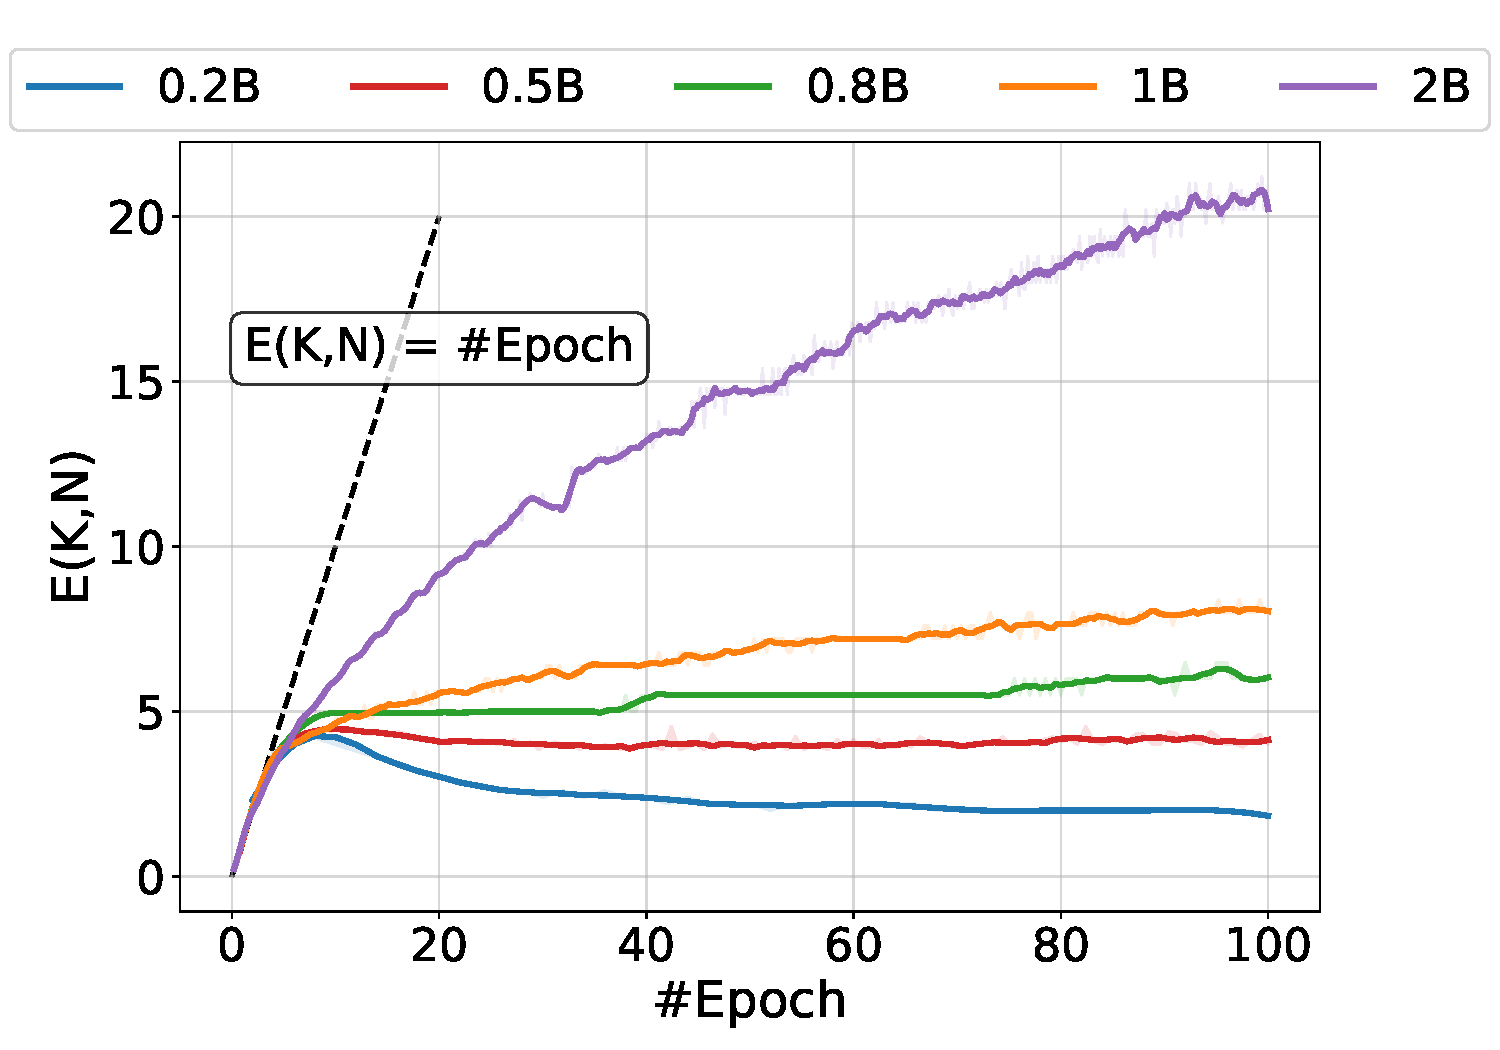
\includegraphics[width=\linewidth]{figs/E_k_smoothed_shaded.pdf}
        %\caption{The effective reuse rate $E(K,N)$ as a function of the epoch number $K$.}
        \caption{$E(K,N)$ as a function of $K$.}
        % \caption{The effective reuse rate $E(K,N)$ as a function of the number of training epochs $K$ for varying fresh data sizes $N$. The shaded regions represent the variability from the smoothed trend in different epochs.}
        \label{fig:ek-k}
    \end{subfigure}  
    \hfill
    \begin{subfigure}[t]{0.32\linewidth}
        % 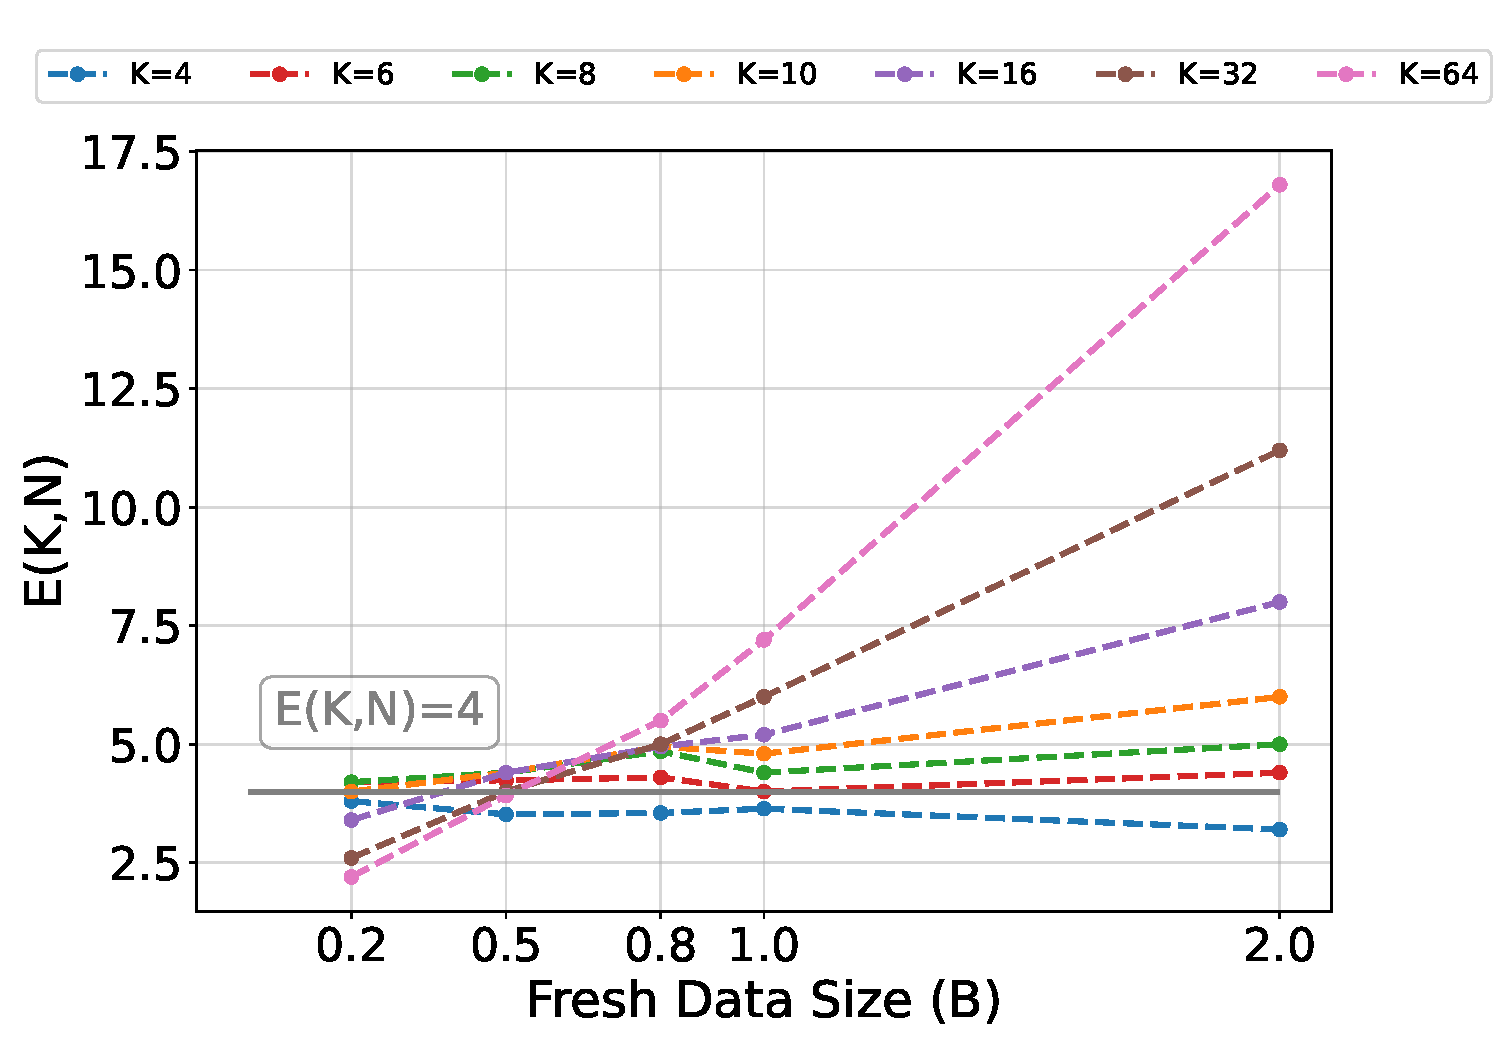
\includegraphics[width=\linewidth]{figs/E_k_over_fresh_data_size.pdf}
        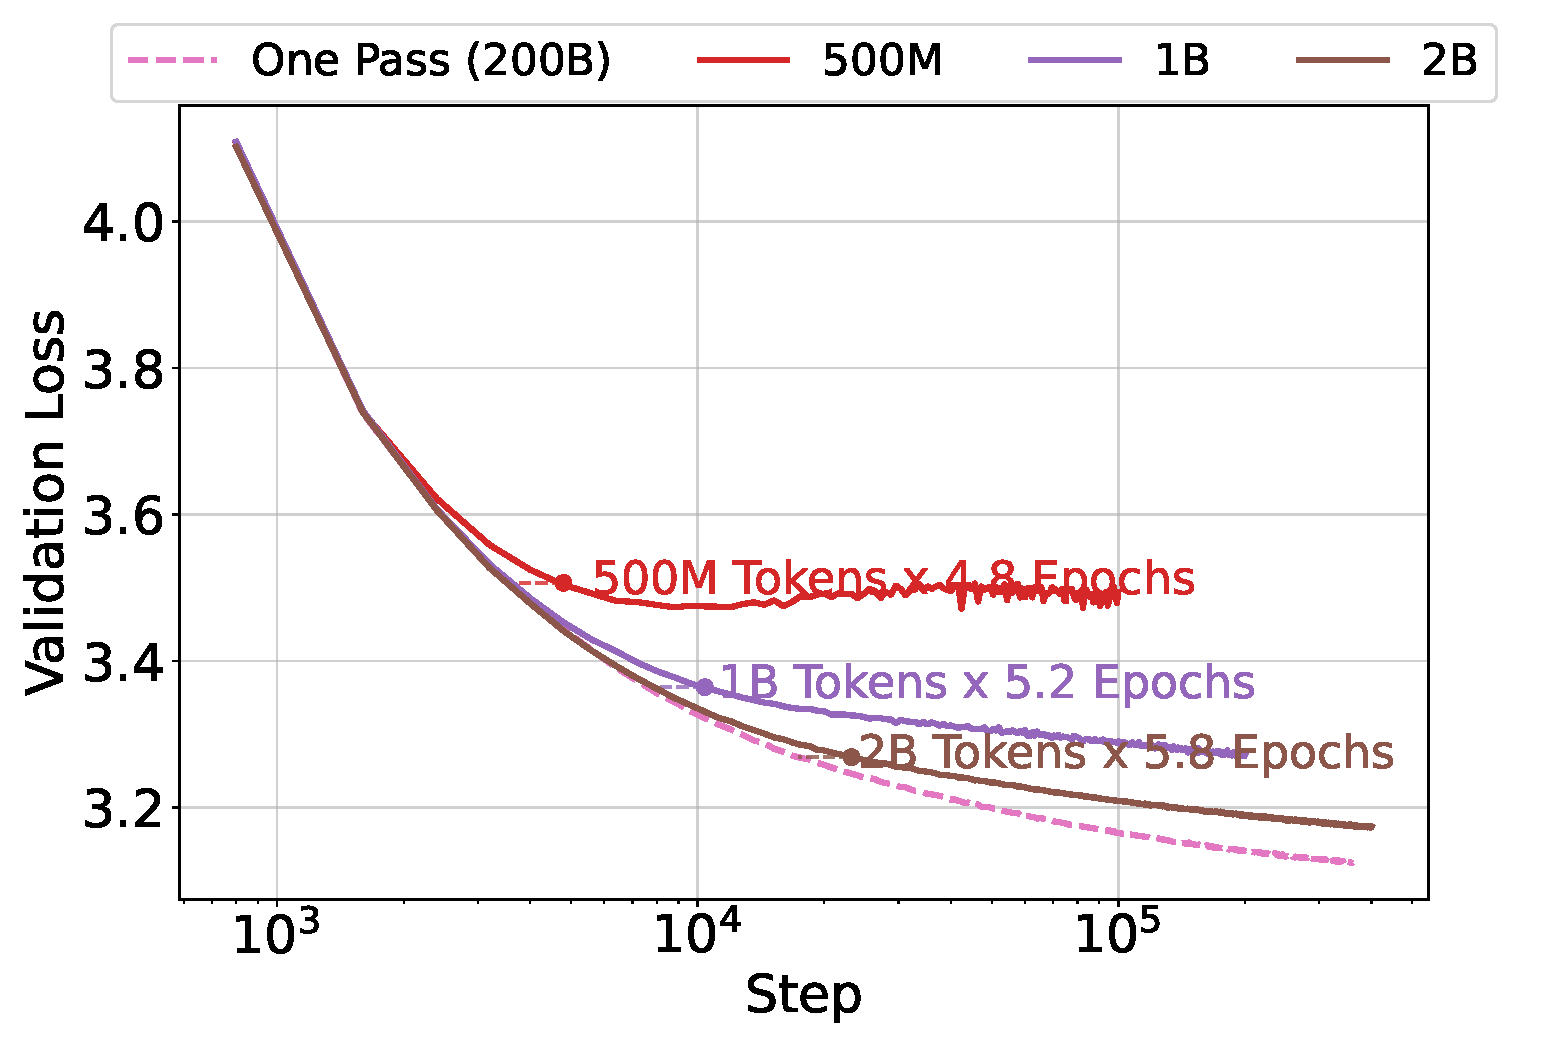
\includegraphics[width=\linewidth]{figs/loss_over_step_improved_ws3_ratio0.75_alpha0.9_exp.pdf}
        %\caption{Training loss as a function of training steps for different fresh data sizes.}
        \caption{Validation loss of one-pass and multi-epoch training runs.}
        \label{fig:loss-step}
    \end{subfigure}
    \hfill
    \begin{subfigure}[t]{0.33\linewidth}
        % 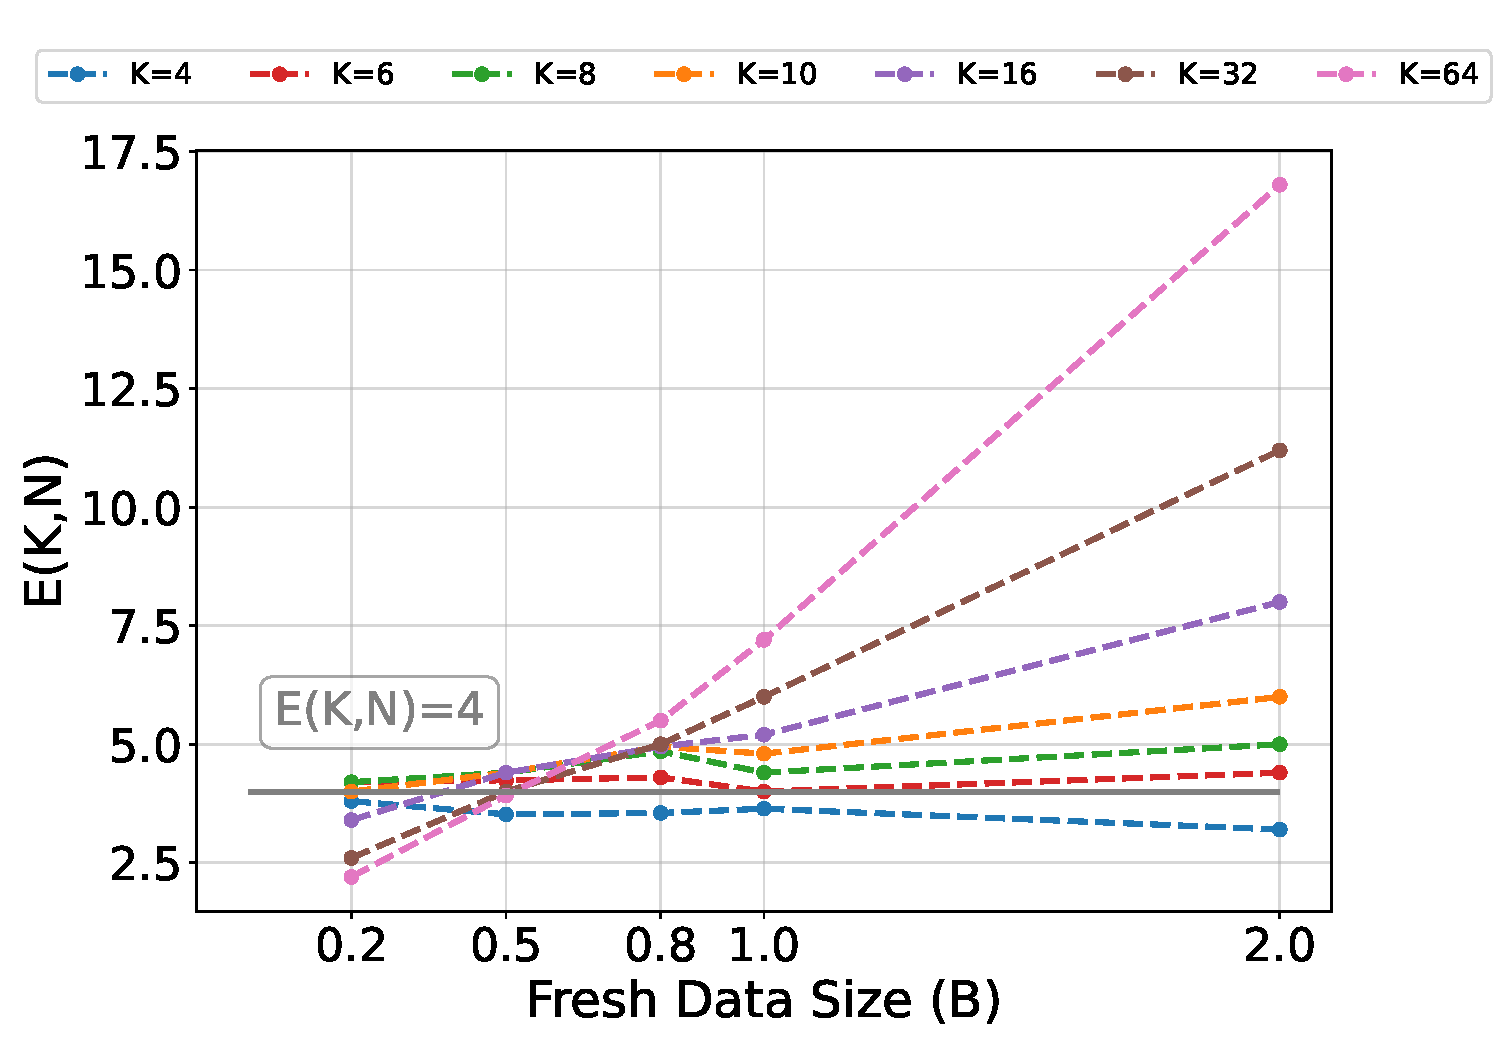
\includegraphics[width=\linewidth]{figs/E_k_over_fresh_data_size.pdf}
        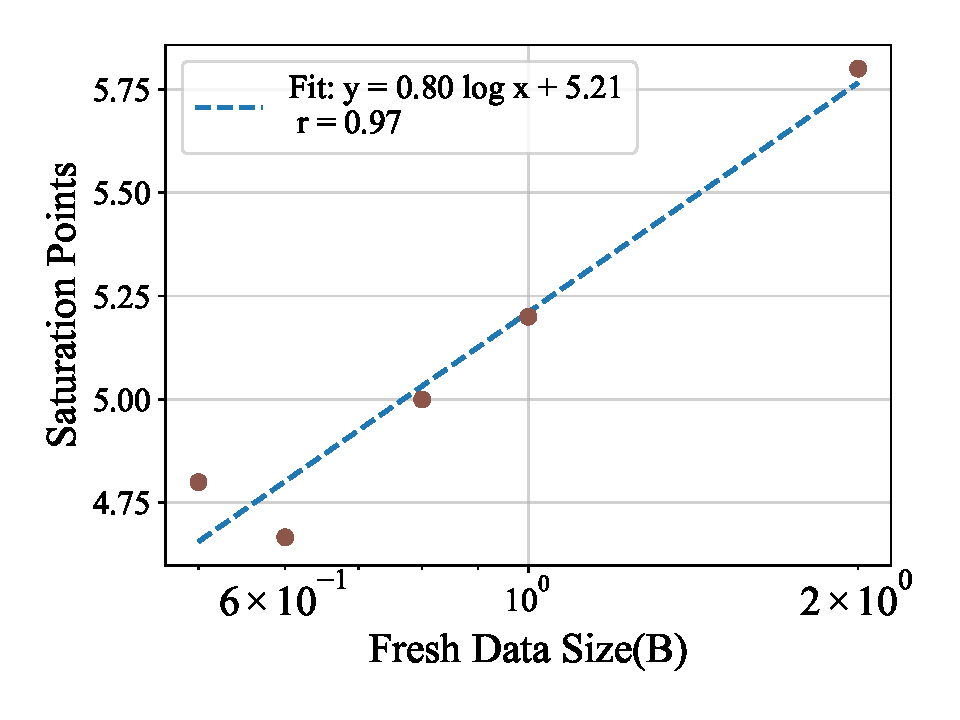
\includegraphics[width=\linewidth,trim=0 0.22in 0 0,clip]{figs/E_KN_vs_N_ws3_ratio0.75_alpha0.9_exp.pdf}
        \caption{The saturation points grows linearly with $\log N$.}
        %\caption{The saturation points $K(\lambda,N)$ as a function of the dataset size N.}
        \label{fig:ek-n-saturation point}
    \end{subfigure}
    \caption{\small Our LLM experiments show that larger datasets can be repeated more.
    \textbf{(a)} The effective reuse rate $E(K, N) \approx K$ when $K$ is small, but eventually saturates at certain number of epochs. \textbf{(b)} The saturation point shifts to larger $K$ as the dataset size increases. \textbf{(c)} Empirically, the saturation points scales linearly with $\log N$.} \label{fig:main-llm}
    %The effective reuse rate $E(K,N)$ over $K$ and training curves in our language model experiments. \Cref{fig:ek-k} shows that $E(K,N)\approx K$ when $K$ is small, to be specific, $K\leq4$. \Cref{fig:loss-step} plots the points where $E(K,N)=0.8K$ under different configurations, and we define the corresponding $E(K,N)$ as the saturation points. In \Cref{fig:ek-n-saturation point}, we observe that the saturation points increases as $N$ increases, indicating that larger datasets can be repeated more.}
    % \kaifeng{you didn't mention figure c}}
    % \caption{}
    % \caption{\textbf{Left:} Training loss progression over training steps. \textbf{Right:} The saturated effective reuse rate $E(K,N)$ in relation to the size of the fresh dataset $N$.}
    \vspace{-0.1in}
\end{figure}

%Then we define the minimum $N'$ such that $\mathcal{L}(1, N') \leq \mathcal{L}(K, N)$, and interpret the ratio $E(K, N) = N'/N$ as the effective reuse rate of the data (see the detailed version in Definition~\ref{def:E_K}).

In a recent study of scaling laws for multi-epoch training, \citet{muennighoff2023scaling} encountered this question and proposed an empirical approximation: $N'(K, N) = \left(1 + R^* (1 - e^{-(K-1)/R^*})\right) \cdot N$,
%Recently, \citet{muennighoff2023scaling} provided an empirical approximation to this key quantity.
%Previous work has provided empirical approximations to this key quantity.
%In particular, \citet{muennighoff2023scaling} proposed to approximate the effective dataset size as
where $R^*$ is a fitted constant ($R^* \approx 15.39$ in their experiments).
This formula suggests that the benefit of repetition grows with $K$ but saturates exponentially at $(1 + R^*) \cdot N$ as $K$ increases. While supported by some empirical evidence in their study, this approximation still leads to a noticeable gap between scaling law predictions and empirical results (see Figure 3 in their paper). Moreover, the formula implies that the ratio $E(K,N) = N'(K, N)/N$ is independent of $N$, so the benefit of repeating the dataset $K$ times is equivalent to increasing its size by a factor that depends only on $K$, regardless of how large $N$ is. It remains unclear to what extent this independence holds in general.


%though it still leaves a noticeable gap between predicted scaling behavior and observed performance, and critically assumes that the ratio $N'(N, K)/N$ is independent of $N$. 

\paragraph{Our Contributions.}
In this paper, we approach the above question on the effective reuse rate of data in the setting of linear regression, a setting that is simple enough to reveal the key mechanisms of data reuse, while still tractable for precise analysis under stochastic gradient descent (SGD).
We provide a theoretical characterization of $E(K, N)$ in various regimes, and point out a neglected factor in the empirical study of \citet{muennighoff2023scaling}: the effective reuse rate depends not only on the number of epochs $K$, but also on the dataset size $N$.
In fact, we show both theoretically and empirically that \textbf{larger datasets can be repeated more}.
%in the setting of linear regression, which is simple enough to reveal the key mechanisms of data reuse, while still tractable for precise analysis under stochastic gradient descent (SGD).
%present a theoretical analysis on the scaling behavior of multi-epoch training in linear regression, and
%provide a theoretical characterization of how $E(K, N)$ depends jointly on $K$ and $N$, complementing prior empirical observations with a principled perspective.
%increase the effective dataset size under one-pass training?}
% \begin{center}
%     \textit{To what extent does training for $K$ epochs on $N$ samples increase the effective dataset size under one-pass training?}
% \end{center}
% \haodong{keep it or not, put it in the line}
% \begin{align}
%     N' = \left(1 + R^* (1 - e^{-(K-1)/R^*})\right) \cdot N,\label{equ:data-constrained-EK}
% \end{align}
%\haodong{rephrase the following paragraph Binghui}
% In contrast, our analysis provides a theoretical characterization of how $E(K, N)$ depends jointly on $K$ and $N$, complementing prior empirical observations with a principled perspective.
% To our knowledge, this work constitutes the first systematic investigation of data scaling laws in the multi-epoch training regime. 
% In this work, under a linear regression setup, we theoretically analyze the data scaling behavior in the multi-epoch training regime. 
%We approach this question in the setting of linear regression, which is simple enough to reveal the key mechanisms of data reuse, while still tractable for precise analysis under stochastic gradient descent (SGD). This makes it a natural testbed for developing a theoretical understanding of multi-epoch scaling. 
%Specifically, we focus on two cases: the strongly convex setting and the high-dimensional setting with a Zipf-law data distribution. 
Our main contributions are as follows:
\begin{enumerate}
\item In~\Cref{sec:strongly_convex}, we analyze multi-epoch SGD for linear regression under strong convexity.
We show that when $K$ is small, $E(K, N) \approx K$, so every new epoch leads to a linear gain. As $K$ increases, $E(K, N)$ saturates at a problem-dependent value of order $\Theta(\log N)$, suggesting that larger datasets can be repeated for more epochs before the marginal benefit vanishes.

\item In~\Cref{sec:one_hot}, we go beyond the strongly convex case and study a class of Zipf-law distributed data, and show that $E(K, N)$ exhibits a similar scaling behavior to the strongly convex case, except that the saturation point scales as a power of $N$ instead of $\log N$.

\item Technically, we derive the optimal learning rate (Lemma~\ref{thm:convex-opt-lr}) for multi-epoch SGD in linear regression and its corresponding approximation formula for the expected excess risk up to an $o(1)$ multiplicative error (Lemma~\ref{thm:convex-L-estimate}). These results may be of independent interest.

\item In~\Cref{sec:experiments}, we conduct LLM pretraining experiments with up to $200$B repeated tokens.
Consistent with our theoretical findings, the empirical results show that $E(K, N) \approx K$ for small $K$, but eventually saturates at an epoch number that scales linearly with $\log N$. 
See also~\Cref{fig:main-llm} for details.
\end{enumerate}

%Our empirical results show that $E(K, N) \approx K$ for small $K$ 
%Similar to our findings in the strongly convex case of linear regression, the saturation point scales linearly with $\log N$.
%We establish  characterization of multi-epoch data scaling in linear regression. We show that $E(K, N) \approx K$ for small $K$, reflecting nearly linear gains from repetition, while for large $K$ the effective reuse rate saturates at an $N$-dependent level: proportional to $\log N$ in the strongly convex case and to $N^\alpha$ (for some $\alpha \in (0,1)$) in the Zipf-law case. This reveals that larger datasets can be repeated more effectively, with the saturation point determined by the problem setup.
%\item We technically provide the first theoretical characterization of the optimal learning rate for multi-epoch SGD in linear regression. This is enabled by a new approximation formula for the expected excess risk up to an $o(1)$ multiplicative error (Lemma~\ref{thm:convex-L-estimate}), which also allows for a tractable analysis of optimal learning rate schedules (Lemma~\ref{thm:convex-opt-lr}). These technical results may be of independent interest.
%This provides direct evidence for our main conclusion: larger datasets can be repeated more.
%We empirically validate our theoretical predictions through LLM pre-training experiments. The results confirm that $E(K, N) \approx K$ for small $K$, and that for fixed $K$, the effective reuse rate increases monotonically with $N$. This provides direct evidence for our central conclusion: larger datasets can indeed be repeated more effectively.
% Our main contributions can be summarized as follows:
% \begin{enumerate}
%     \item 
%     In Section~\ref{sec:strongly_convex}, our analysis in the strongly convex case of linear regression shows that, if the learning rate is optimally tuned, $E(K, N)$ grows proportionally to $\log N$ and saturates at $K$ when $\log N \gg K$ (Theorem~\ref{thm:convex-E_K}).
%     \item Technically, we provide an approximation formula for the expected excess risk up to $o(1)$ multiplicative error~(Lemma~\ref{thm:convex-L-estimate}), which enables a tractable analysis of the optimal learning rate (Lemma~\ref{thm:convex-opt-lr}). These results may be of independent interest.
%     \item 
%     In ~\Cref{sec:one_hot}, we consider a solvable case with a power-law spectrum structure. Under this setting, we prove that $E(K, N)$ exhibits a similar scaling behavior to the strongly convex case, but it has different saturation points for different spectra (\Cref{thm:one-hot-E_K-v2} and \Cref{thm:one-hot-E_K-log-spectrum}).
%     \item 
%     In Section~\ref{sec:experiments}, we validate our theoretical implications in the context of language model pretraining. Our findings indicate that the effective reuse rate approximates the epoch number for small numbers of repetitions. Furthermore, for a fixed number of epochs, the effective reuse rate increases monotonically with the fresh data size (\Cref{fig:ek-k,fig:ek-data,fig:loss-step}). This supports the conclusion that larger datasets can be repeated more effectively.
% \end{enumerate}

% When developing scaling laws for multi-epoch training,~\citet{muennighoff2023scaling} encountered this question and proposed the following approximation for the effective data size $N'$: 
% % $N' = \left(1 + R^* (1 - e^{-(K-1)/R^*})\right) \cdot N$,
% \begin{align}
%     N' = \left(1 + R^* (1 - e^{-(K-1)/R^*})\right) \cdot N,\label{equ:data-constrained-EK}
% \end{align}
% where $R^*$ is a fitted constant ($R^* \approx 15.39$ in their experiments). This formula suggests that the benefit of repetition grows with $K$ but saturates exponentially at $(1 + R^*) \cdot N$ as $K$ increases. While supported by some empirical evidence in their study, this approximation still leads to a noticeable gap between scaling law predictions and empirical results (see Figure 3 in their paper).
% Moreover, the formula implies that the ratio $N'/N$ is independent of $N$, so the benefit of repeating the dataset $K$ times is equivalent to increasing the dataset size by a factor that depends only on $K$, regardless of how large $N$ is. It remains unclear to what extent this independence holds in general.

%Notably, the formula implies that the ratio $N' / N$ is independent of $N$. This means that no matter how large the dataset size $N$ is, the benefit of repeating the dataset $K$ times is equivalent to increasing the dataset size by a factor that depends only on $K$.
%and it is also unclear to what extent this formula holds more broadly.

%Notably, the formula implies that the fraction $N' / N$ is always a constant in $N$, and thus no matter how large the dataset size $N$ is, repeating the dataset $K$ times always benefits the performance like multiplying the dataset size by a factor only depending on $K$.



%This formula assumes that when repeating the dataset, the effective dataset size grows with the number of epochs $K$, but the growth exponentially saturates to $(1 + R^*) \cdot N$ as $K$ becomes much larger than $R^*$. However, although some empirical evidence is presented in~\citet{muennighoff2023scaling}, it is not clear whether this form of $N'$ is universally applicable to all practical settings. In particular, in this formula, 


% \paragraph{Our Contributions.}
% In this paper, we present a theoretical analysis on the scaling behavior of multi-epoch training and examine how $N'/N$ really behaves in linear regression problems.
% Formally, we define the {\it effective reuse rate} $E(K, N)$ of the data as $N'/N$, the ratio of the effective dataset size $N'$ to the original dataset size $N$ for $K$-epoch training (see the formal definition in Definition~\ref{def:E_K}). Our main contribution can be summarized as follows:
% \begin{enumerate}
%     \item 
%     In Section~\ref{sec:strongly_convex}, our analysis in the strongly convex case of linear regression shows that, if the learning rate is optimally tuned, $E(K, N)$ grows proportionally to $\log N$ and saturates at $K$ when $\log N \gg K$ (Theorem~\ref{thm:convex-E_K}).
%     %\item Technically, we provide an approximation formula for the expected excess risk up to $o(1)$ multiplicative error~(Lemma~\ref{thm:convex-L-estimate}), which enables a tractable analysis of the optimal learning rate (Lemma~\ref{thm:convex-opt-lr}). These results may be of independent interest.  % \kairong{What is ``population excess risk''? Is it a well-known term?} \kairong{Fine, find it in Preliminary.}
%     %Then, based on the approximately optimal learning rate for one-pass SGD and the designed learning rate for multi-epoch SGD, we show that $E(K, N)$ grows proportionally to $\log N$ and saturates at $K$ when $\log N \gg K$ (Theorem~\ref{thm:convex-E_K}).
%     \item 
%     In ~\Cref{sec:one_hot}, we consider a solvable case with a power-law spectrum structure. Under this setting, we prove that $E(K, N)$ exhibits a similar scaling behavior to the strongly convex case, but it has different saturation points for different spectra (\Cref{thm:one-hot-E_K-v2}).%, \Cref{thm:one-hot-E_K-log-spectrum}, and \Cref{thm:one-hot-E_K-b=0}).
%     \item 
%     In Section~\ref{sec:experiments}, we validate our theoretical implications in the context of language model pretraining. Our findings indicate that the effective reuse rate approximates the epoch number for small numbers of repetitions. Furthermore, for a fixed number of epochs, the effective reuse rate increases monotonically with the fresh data size (\Cref{fig:ek-k,fig:ek-data,fig:loss-step}). This supports the conclusion that larger datasets can be repeated more effectively.
% \end{enumerate}

%Noting that $N'$ may take the form of $N$ multiplied by a factor, in this paper, we stu
%provide an extensive empirical study of the scaling behavior of multi-epoch training, and propose that training a model on a dataset of size $N$ for $K$ epochs leads to a loss similar to that of training on a dataset of size $N'$ in the one-pass regime, where the {\it effective dataset size} $N'$ is given by
% \begin{align}
%     N' = \left(1 + R^* (1 - e^{-(K-1)/R^*})\right) \cdot N,
% \end{align}

%where $R^*$ is a constant to be fit from empirical experiments ($R^* \approx 15.39$ in their experiments). This formula assumes that when repeating the dataset, the effective dataset size grows with the number of epochs $K$, but the growth exponentially saturates to $(1 + R^*) \cdot N$ as $K$ becomes much larger than $R^*$. However, although some empirical evidence is presented in~\citet{muennighoff2023scaling}, it is not clear whether this form of $N'$ is universally applicable to all practical settings, and whether $R^*$ is indeed a constant independent of other factors.


%the form of $R^*$ and its dependence on the dataset size, model size, and number of passes $K$ is not well understood.
%, assumed to be independent of the dataset size, model size, and number of passes $K$ 

%That is, the 
%the effective dataset size under repetition can be expressed as $C_K \cdot N$, where $C_K$ is a constant potentially dependent on the number of passes $K$, but its form and behavior remain unclear. 
%study the effect of ME training on scaling laws and observe that for a small number of epochs, repeated data can approximate the benefits of fresh data. However, their findings also reveal a clear degradation: as the number of epochs increases—e.g., beyond four passes over 900 billion tokens—performance gains diminish, and the marginal utility of additional compute approaches zero.

%\citet{charton2024emergent} and 

%These results highlight the empirical limitations of ME training at scale. Yet, despite its practical relevance, our theoretical understanding of how data repetition influences scaling laws remains limited. In particular, there is a lack of rigorous derivations capturing this behavior. For example, \citet{muennighoff2023scaling} suggest that the effective dataset size under repetition can be expressed as $C_K \cdot N$, where $C_K$ is a constant potentially dependent on the number of passes $K$, but its form and behavior remain unclear. Moreover, existing scaling formulas derived in the OP regime fail to extrapolate accurately as $K$ becomes large.

%In this paper, we study the scaling behavior of multi-epoch training from a theoretical perspective. 
%Concretely, 


%To study how $N'$ behaves in the data-constrained regime, we introduce the notion of effective reuse rate, which we define as the factor by which the dataset must grow under one-pass training to match the test loss of multi-epoch training.
%denoted $E(K, N)$


%, as a principled measure of how repeated exposure to a finite dataset contributes to training. This term generalizes the idea of effective dataset size and serves as a core quantity for analyzing scaling behavior in the data-constrained regime.


%Motivated by these limitations, we revisit the problem of multi-epoch training from an information-theoretic perspective. We introduce the notion of effective reuse rate, denoted $E(K, N)$ (see the formal definition in Definition~\ref{def:E_K}), as a principled measure of how repeated exposure to a finite dataset contributes to training. This term generalizes the idea of effective dataset size and serves as a core quantity for analyzing scaling behavior in the data-constrained regime.

%\begin{center}
%\textit{Can we provably characterize the scaling behavior of $E(K, N)$ in the data-constrained regime?}
%\end{center}


% \kaifeng{reorganize into bullet points}
% In this paper, we study the theory of the scaling behavior differences between one-pass (OP) and multi-epoch (ME) training in two classical linear regression setups. We provide a theoretical framework for analyzing \( E(K, N) \) under solvable models, offering insight into how compute and data interact when data reuse is unavoidable. The first model we consider is a finite-dimensional, strongly convex linear regression problem, for which we apply both OP stochastic gradient descent (SGD) and ME SGD algorithms. We perform a fine-grained analysis of the population excess risk for both optimization algorithms and analyze the scaling behavior of these two algorithms under a selected learning rate, achieving an approximately optimal convergence rate for OP SGD. The second problem we investigate is an infinite-dimensional linear regression problem, with a power spectrum assumption on the covariance matrix, which is commonly used in scaling law theory~\citep{lin2024scaling,luo2025multi}. We derive matching upper and lower bounds for the loss obtained by both ME and OP SGD optimization algorithms, thus providing an expression for the scaling law.


%\paragraph{Motivation.} The motivation of our theory is to derive the effective number of epochs. In other words, if we run an ME SGD for $K$ epochs, how many effective epochs would be required for the corresponding OP to achieve the saME population excess risk as ME? Specifically, considering an ME SGD optimization algorithm with dataset size $N$, and number of epochs $K$, and the ME SGD after $T=KN$ steps achieves a population excess risk $L_T$, correspondingly, we have another OP SGD, with unique data in every step, runing $T'$ steps, with population excess risk $L'_{T'}$. Now we select the minimal $T'$ such that $L'_{T'} \le L_T$, and we define the term $E_K=T'/N$ as the effective number of epochs, which characterizes the difference between ME and OP in their scaling behaviors.

%\paragraph{Challenge.}\haodong{it is typically hard to directly analyze the loss formula and get the clean expression of $E_K$. Also, the iMEact of random shuffling is extreMEly tedious to capture.}

% \paragraph{Our Contribution.}
% \begin{itemize}
%     \item Considering random shuffling, give a mathematical fraMEwork for multi-epoch SGD in standard finite diMEnsion strongly convex linear regression, provide results like: loss approximation, with tools in matrix concentration, asyMEtotically optimal learning rate, and effective number of epochs.
%     \item In power spectrum assuMEtion (non-strongly convex case) with top $d$ sketching matrix $S$, we get: loss approximation (scaling law), and 
% we give an analysis of the effective number of epochs with soME learning rate.
% \end{itemize}

% Our main contributions are sumMErized as follows.
% \begin{itemize}
%     \item 
%     formalize $E_K$ xxx
%     \item 
%     strongly convex linear regression xxx
%     \item 
%     one-hot power law xxx
%     \item 
%     in real-world experiMEnts xxx
% \end{itemize}

\section{Related Work} \label{sec:related}

\paragraph{Data Reuse in LLM Pre-Training.} Empirically, there is a long debate over the effect of data reuse in LLM pre-training. Some works~\citep{lee2021deduplicating,hoffmann2022training,hernandez2022scaling,wang2023data} suggested it may be harmful, while some works~\citep{taylor2022galactica} reported the benefit of data reuse when the number of epochs is small ($K \le 4$).
% \kaifengclaw{Typo/consistency: 'some work' -> 'some works'; and 'data reusing' is better unified as 'data reuse'.} 
\citet{xue2023repeat} then discovered a degradation phenomenon in multi-epoch training and investigated relevant factors and regularization methods to tackle it. \citet{muennighoff2023scaling} trained LLMs under different configurations and also found that reusing data is as good as using fresh data in the first few epochs. Yet, as the number of epochs increases, the returns for repetitions diminish. In our work, from a theoretical perspective, we rigorously analyze the effect of data reuse using non-asymptotic techniques, and we define and calculate the effective reuse rate under two cases, shedding light on the theoretical understanding of data reusing in LLM pre-training.
% \kaifengclaw{Tense/style: keep consistent tense in related work (e.g., present tense: 'analyze', 'define', 'calculate').}

\paragraph{Comparison with \citet{lin2025improved}.} A recent study on linear regression with data reusing~\citep{lin2025improved} is among the most relevant to our results. They showed that when the number of epochs is relatively small (smaller than some power of the dataset size), the order of loss remains the same as one pass SGD for the same iterations, which aligns with our results. However, their results only imply that $E(K,N) = \Theta(K)$ for small $K$, while our analysis directly gives the explicit loss characterization with $o(1)$ relative error bound and a more exact description of the effective reuse rate, which reflects the data reusing scaling behaviour. Our analysis is across various problem setups, and further shows the general scaling trend of data reusing under different problem setups.

%\tingkai{Read all the papers and separate the papers; emphasize that some paper consider the linear regression setting; more papers to cite}
\iffalse
\paragraph{Data Reuse in LLM Pre-Training.} 
% As fresh data is becoming scarce \citet{villalobos2024run}, data reuse is getting more and more attention and remains a research hotspot empirically and theoretically. Some works have focused on the downside of data reuse, for example, 

%There are many empirical discussions about the effect of data reusing in Large Language Model (LLM) training. 
Some previous works suggested that data reuse for LLM training may be harmful~\citep{lee2021deduplicating,hoffmann2022training,hernandez2022scaling,wang2023data}. However, \citet{taylor2022galactica} observed that reusing pre-training data up to $4$ epochs for a $120$B model has a positive impact. \citet{xue2023repeat} then discovered a degradation phenomenon in multi-epoch training and investigated relevant factors and regularization methods to tackle it. \citet{muennighoff2023scaling} trained large language models under different configurations and found that reusing previous data is as good as using new fresh data in the first few epochs. Yet, as the number of epochs increases, the returns for repetitions diminish. 
% \haodong{check empirical papers: some LLM empirical papers show that data repeating and match fresh data only when the number of epochs is very small. Some theory - > better for repeating, but observed on some synthetic setting}
Besides the real-world LLM pre-training regime, many works also reported the improvement of data reusing under synthetic settings empirically~\citep{charton2024emergent,kazdan2024collapse} or theoretically~\citep{zucchet2025emergence,dandi2024benefitsreusingbatchesgradient,arnaboldi2025repetitaiuvantdatarepetition}.  
% \citet{charton2024emergent}studied the performances of transformers on three types of math problems and concluded that data repetition is necessary. 
% Specifically, on the theoretical side, a line of work developed tools in mean field theory and gave results on the limitations of data reuse under some synthetic settings. \citet{dandi2024benefitsreusingbatchesgradient} considered a function-learning problem with multi-pass gradient descent that reuses the batches multiple times. This optimizer performed efficiently and overcame the constraints given by the information exponent \citep{BenArous2021} and leap exponent \citep{abbe2023sgd}, even for functions that does not satisfy the staircase property \citep{abbe2024mergedstaircasepropertynecessarynearly}. 
% Furthermore, \citet{arnaboldi2025repetitaiuvantdatarepetition} investigated a modification of single-pass gradient descent where data could be reused twice. They observed a drastic improvement in computational efficiency. 
In our work, we rigorously analyzed the effect of data reuse using non-asymptotic techniques, and we defined and calculated the effective reuse rate under two cases, shedding light on the theoretical understanding of data reusing in LLM pre-training.

% \paragraph{Empirical Scaling Laws.}
% Scaling laws that reveal the relationships between training loss and other factors such as model size, data size and compute budget have always been an extensive area of research. \citet{kaplan2020scaling} is the first to propose a power-law decay formula w.r.t. data size and model size in the context of training transformer-based large language models. Since then, literature have been focusing on fitting scaling laws under different settings ... . \citet{hoffmann2022training} put forward a Chinchilla law that is different from Kaplan scaling laws, and proposed methods to allocate data and model size under a given compute budget. \citet{muennighoff2023scaling} fitted a more-complex scaling law which takes the number of training epochs into consideration.
%\haodong{ rephrase the following scaling law reference}

\paragraph{Empirical Findings on Scaling Laws.} Scaling laws reveal the relationships between large-scale model training loss and various factors such as model size, data size, and compute budget. These laws were initially observed by \citet{hestness2017deep}, but gained significant influence through the work of \citet{kaplan2020scaling}, and have since been further developed in a series of studies \citep{henighan2020scaling, hoffmann2022training, zhai2022scaling, kadra2023power, aghajanyan2023scaling, muennighoff2023scaling, bi2024deepseek, shuai2024scaling, kumar2024scaling, tissue2024scaling, luo2025multi}. %Notably, \citet{hoffmann2022training} introduced the Chinchilla Law, which proposes an optimal scaling strategy under a fixed compute budget. Additionally, \citet{tissue2024scaling} and \citet{luo2025multi} explored scaling laws with learning rate schedules (LRSs) based on empirical observations. 
Notably, \citet{muennighoff2023scaling} further refined these models by incorporating the number of training epochs into a more complex scaling law, which empirically describes the effect of data reuse. In our work, we provide a theoretical analysis of how the effective reuse rate $E(K,N)$ relies on the epoch number $K$ and fresh data size $N$, highlighting the role of $N$ in the scaling behavior of $E(K,N)$, a factor that was overlooked in \citet{muennighoff2023scaling}. 

% \paragraph{Theory of Scaling laws.}
% There are many existing works that interpreted the mechanism behind the scaling laws ... . \citet{sharma2020neuralscalinglawdimension} considered a toy model and showed that $\cL \propto \frac{1}{N^{\frac{4}{d}}}$, where $d$ is the intrinsic dimension. \citet{Bahri_2024} and \citet{bordelon2024dynamicalmodelneuralscaling} both analyzed a linear teacher-student model setting with a power-decay parameter prior. They proposed theories for scaling laws based on statistical heruistics. \citet{bordelon2025featurelearningimproveneural} developed a solvable model of neural scaling laws and defined regimes according to task difficulties. Meanwhile, other works considered more complicated settings and gave more rigorous mathematical proofs. \citet{jain2024scalinglawslearningreal} studied how data from other sources affect the test error of models and their scaling laws. \citet{paquette202543phasescomputeoptimalneural} identified different phases for a PLRF model in the compute-limited, infinite-data scaling law regime, and they discovered different scaling exponents in different phases. \citet{lin2024scaling} proved a scaling law using a PLRF model with an online SGD scheme with a geometrically decaying stepsize non-asymptotically. However, these scaling law papers failed to consider the impact of data reuse. In contrast, we proved matching upper and lower risk bounds in two settings for multi-epoch training.
% \paragraph{Theory of Multi-Pass SGD.}
% Shuffling is a common practice in machine learning, however, theoretical literature on SGD with shuffling is limited. 

%\haodong{emphasize that the linear regression setting is attracting more and more interest}
\paragraph{Theoretical Explanations for Scaling Laws.} A series of studies \citep{sharma2020neuralscalinglawdimension,hutter2021learning,maloney2022solvable,wei2022more,jain2024scalinglawslearningreal,michaud2024quantization,nam2024exactly,atanasov2024scaling,dohmatob2024tale,bahri2024explaining,bordelon2024dynamical,lin2024scaling,paquette202543phasescomputeoptimalneural,bordelon2024feature,zhang2024does,ferbach2025dimension,li2025fsl} have sought to theoretically explain scaling laws from various perspectives. Among these, recent works \citep{bordelon2024dynamical,paquette202543phasescomputeoptimalneural,lin2024scaling,bordelon2024feature} have analyzed scaling laws by tracking the training dynamics of SGD through linear regression setup. Specifically, \citet{bordelon2024dynamical} investigated a full-batch gradient flow setup, while \citet{paquette202543phasescomputeoptimalneural} and \citet{bordelon2024feature} focused on online SGD with a sufficiently small constant learning rate. Additionally, \citet{lin2024scaling} studied a geometric decaying learning rate schedule (LRS) \citep{ge2019step,wu2022iterateriskboundssgd}. Recently, \citet{li2025fsl} proposed a functional scaling law that characterizes the loss dynamics for general LRSs. However, these scaling law studies did not account for the impact of data reuse. In contrast, our work examines the scaling behavior of multi-epoch SGD training within the context of a linear regression setup. 

\paragraph{Comparison with \citet{lin2025improved}.} A recent study on linear regression with data reusing~\citep{lin2025improved} is among the most relevant to our results. They showed that when the number of epochs is relatively small (some power of the dataset size), the order of loss remains the same as one pass SGD for the same iterations, which aligns with our results. However, their results only imply that $E(K,N) = \Theta(K)$ for small $K$, while our analysis directly gives the explicit loss characterization with $o(1)$ relative error bound and a more exact description of the effective reuse rate, which reflects the data reusing scaling behaviour. Our analysis is across various problem setups, and further shows the general scaling trend of data reusing under different problem setups.

% A recent related paper \citet{lin2025improved} studies the scaling law in the data reuse regime and showed that the loss under data reusing can improve the exponents in the scaling law for a class of regression problems. Their analysis considers the shuffling with replacement, and is hard to derive an explicit characterization of the data-resuse efficiency in general linear regression problems.\haodong{point out the defference of Theta and 1 + o(1);why they can iimporve but we cannot}

\paragraph{SGD Analysis in Linear Regression.} %\haodong{mention some scaling law papers} 
The analysis of SGD in linear regression has been extensively studied over the years, encompassing both one-pass and multi-epoch SGD. In the context of one-pass SGD, \citet{zou2021benign,meterez2025simplified} considered an SGD procedure with a constant step size and averaged iterates, offering a sharp risk bound in terms of the eigenvalues of the covariance matrix. \citet{pmlr-v139-gurbuzbalaban21a} examined one-pass SGD with batch size and proved that the distribution of
the SGD iterates will converge to a heavy-tailed
stationary distribution. \citet{zou2022benefitsimplicitregularizationsgd} compared the performance of SGD in the absence of ridge regression. \citet{wu2022iterateriskboundssgd} and \citet{wu2022powerlimitationpretrainingfinetuninglinear} studied SGD in linear regression under covariate shift. \citet{xia2024data} considered SGD updates with noisy gradient and analyzed the perfect deleted point problem. \citet{li2025understanding} considered SGD with exponential moving average in the linear regression setting. For multi-epoch SGD, \citet{lin2019optimalratesmultipassstochastic} examined a scenario in which gradients are sampled uniformly at random and mini-batches are allowed. They analyzed the effects of mini-batch size, number of epochs, and learning rate, carefully combining these parameters to achieve the optimal convergence rate. \citet{pillaudvivien2018statisticaloptimalitystochasticgradient} showed that while single-pass averaged SGD is optimal for a certain class of "easy" problems, multiple passes are required to achieve optimal prediction performance on a different class of "hard" problems, provided that an appropriate step size is chosen. In contrast to the matching upper and lower bounds derived by our theory, however, all the above works were only able to derive an upper bound for the loss.

% In one-pass SGD for linear regression, constant-step-size schedules with iterate averaging yield sharp risk bounds based on covariance eigenvalues (Zou et al., 2021; 2022) and have been studied under covariate shift (Wu et al., 2022). For multi-epoch SGD, optimal rates depend on mini‑batch size, epoch count, and learning rate (Lin et al., 2019), and while averaged single‑pass SGD is optimal for “easy” problems, “hard” problems require multiple passes with tuned step sizes, though only upper loss bounds were previously shown (Pillaud‑Vivien et al., 2018).

% \paragraph{SGD Analysis in Linear Regression.}
% One-pass SGD with constant step size and iterate averaging yields sharp eigenvalue-based risk bounds \citep{zou2021benign}, benefits without ridge regularization \citep{zou2022benefitsimplicitregularizationsgd}, and robustness under covariate shift \citep{wu2022iterateriskboundssgd,wu2022powerlimitationpretrainingfinetuninglinear}. Multi-epoch SGD achieves optimal convergence when mini‑batch size, epoch count, and learning rate are jointly tuned \citep{lin2019optimalratesmultipassstochastic}, and while single-pass averaging suffices for “easy” problems, “hard” problems require multiple passes—though only upper loss bounds are known \citep{pillaudvivien2018statisticaloptimalitystochasticgradient}.
\fi


\vspace{-0.07in}
\section{Preliminaries}
\label{sec:setup}
%In this section, we present our problem setup. In total, we theoretically study the data reuse scaling behavior in linear regression problems.

% \paragraph{Notation.} 
% Throughout this work, we use letters for scalars and bold letters for vectors. We use \( \|\cdot\| \) to denote the \( \ell_2 \)-norm of vectors and the corresponding operator norm of matrices. For any given two sequences $\left\{A_n\right\}_{n=0}^{\infty}$ and $\left\{B_n\right\}_{n=0}^{\infty}$, we denote $A_n=O\left(B_n\right)$ if there exist some absolute constant $C_1>0$ and $N_1>0$ such that $\left|A_n\right| \leq C_1\left|B_n\right|$ for all $n \geq N_1$. Similarly, we denote $A_n=\Omega\left(B_n\right)$ if there exist $C_2>0$ and $N_2>0$ such that $\left|A_n\right| \geq C_2\left|B_n\right|$ for all $n>N_2$. We say $A_n=\Theta\left(B_n\right)$ if $A_n=O\left(B_n\right)$ and $A_n=\Omega\left(B_n\right)$ both holds. We say $A_n = o(B_n)$ (or $A_n \ll B_n$ or $B_n \gg A_n$) if for arbitrary positive constant $C_3 > 0$, there exists $N_3 > 0$ such that $|A_n| < C_3 |B_n|$ for all $n>N_3$. And we also use $A_n \approx B_n$ to denote $A_n = B_n + o(1)$. For two vectors \( \vu \) and \( \vv \) in a Hilbert space, we denote their inner product by \( \langle \vu, \vv \rangle \) or \( \vu^\top \vv \). For two matrices \( \mA \) and \( \mB \) of appropriate dimensions, we define their inner product as \( \langle \mA, \mB \rangle := \tr(\mA^\top \mB) \). Finally, \( \log(\cdot) \) refers to the logarithm with base $e$, where $e$ is the natural exponent.
% \haodong{add notations for big O notation}
\paragraph{Notations.}
%Throughout this work, we use letters for scalars and bold letters for vectors. 
We use \( \|\cdot\| \) to denote the \( \ell_2 \)-norm of vectors and the corresponding operator norm of matrices. 
For two sequences \((A_n)_{n=0}^\infty\) and \((B_n)_{n=0}^\infty\), we write 
\(A_n = O(B_n)\), or alternatively $A_n \lesssim  B_n$, $B_n = \Omega(A_n)$, $B_n \gtrsim A_n$, if there exist constants \(C>0, N>0\) such that \(|A_n|\leq C|B_n|\) for all \(n \geq N\). %We write $A_n = \Omega(B_n)$, or alternatively $A_n \gtrsim  B_n$, if $B_n = O(A_n)$. 
We write $A_n = \Theta(B_n)$, or alternatively $A_n \asymp  B_n$, if both $A_n = O(B_n)$ and $A_n = \Omega(B_n)$ hold.
Moreover, for some variable $n$, we write $A_n = o_n(B_n)$ if for every constant \(c>0\), there exists \(n_0>0\) such that \(|A_n| < c|B_n|\) for all \(n \geq n_0\). In this paper, when $n$ is clear from the context, we write $A_n = o(B_n)$ for short. Furthermore, we write $A_n = \omega(B_n)$ if $B_n = o(A_n)$. For matrices $\mA_1, \mA_2,\dots,\mA_n$, we use $\prod_{l=1}^n \mA_l$ to denote the product $\mA_1\mA_2\dots\mA_n$. We define $\|\boldsymbol{u}\|_{\mS} := \sqrt{\boldsymbol{u}^\top \mS\boldsymbol{u}}$ for any vector $\boldsymbol{u}$ and any positive semi-definite (PSD) matrix $\mS$.

%; and \(A_n \approx B_n\) if \(A_n = B_n + o(1)\). 
% For vectors \(\vu, \vv\) in a Hilbert space, we denote their inner product by \(\langle \vu, \vv \rangle\) or \(\vu^\top \vv\). 
% For matrices \(\mA, \mB\) of compatible dimensions, we define \(\langle \mA, \mB \rangle := \tr(\mA^\top \mB)\). 
% Finally, \(\log(\cdot)\) refers to the natural logarithm with base \(e\).

\paragraph{Linear Regression Problem.} We focus on a linear regression setup, where data point $(\vx,y) \in \mathbb{R}^{d}\times\mathbb{R}$ follows a joint distribution $\mathcal{D}$ and $\|\vx\|\leq D$ for some constant $D$. W.L.O.G., we assume that the covariance matrix of data input is diagonal, i.e., $\mH := \E[\vx\vx^\top] = \diag \left(\lambda_1, \lambda_2, \dots, \lambda_{d}\right) $, where $\lambda_1 \geq \lambda_2 \geq \dots \geq \lambda_{d}$. A direct corollary is that $\lambda_1 \leq D^2$. For a given data input $\vx$, the label $y$ is generated by $y:= \langle \vw^*, \vx \rangle + \xi$, where $\vw^* \in \mathbb{R}^{d}$ is the ground-truth weight and $\xi$ represents the independent random label noise with $\E[\xi] = 0$ and $\E[\xi^2] = \sigma^2$. We aim to train a linear model $f(\vx; \vw):=\langle \vw, \vx \rangle$ to predict the data label, where $\vw \in \mathbb{R}^{d}$ is the trainable parameter. We use MSE-loss $\ell(\vw; \vx, y):=\frac{1}{2}(f(\vx; \vw)-y)^2$ to measure the fitting error. Then, the population loss is defined as $\cL(\vw):= \E_{(\vx, y) \sim \cD}[\ell(\vw;\vx, y)]$. Further we define the excess risk $\cR(\vw) := \cL(\vw) - \frac{1}{2}\sigma^2$, which is the expected population loss minus the irreducible loss $\frac{1}{2}\sigma^2$.
%and the excess risk is defined as $\E_{\vw}\cR(\vw):=  \E_{\vw}\cL(\vw)- \frac{1}{2}\sigma^2$,

% \begin{figure}[t!]
%     \centering
%     \subfigure[$E(K,N)$ v.s.~$K$.%
%       \label{fig:ek-k}]{
%         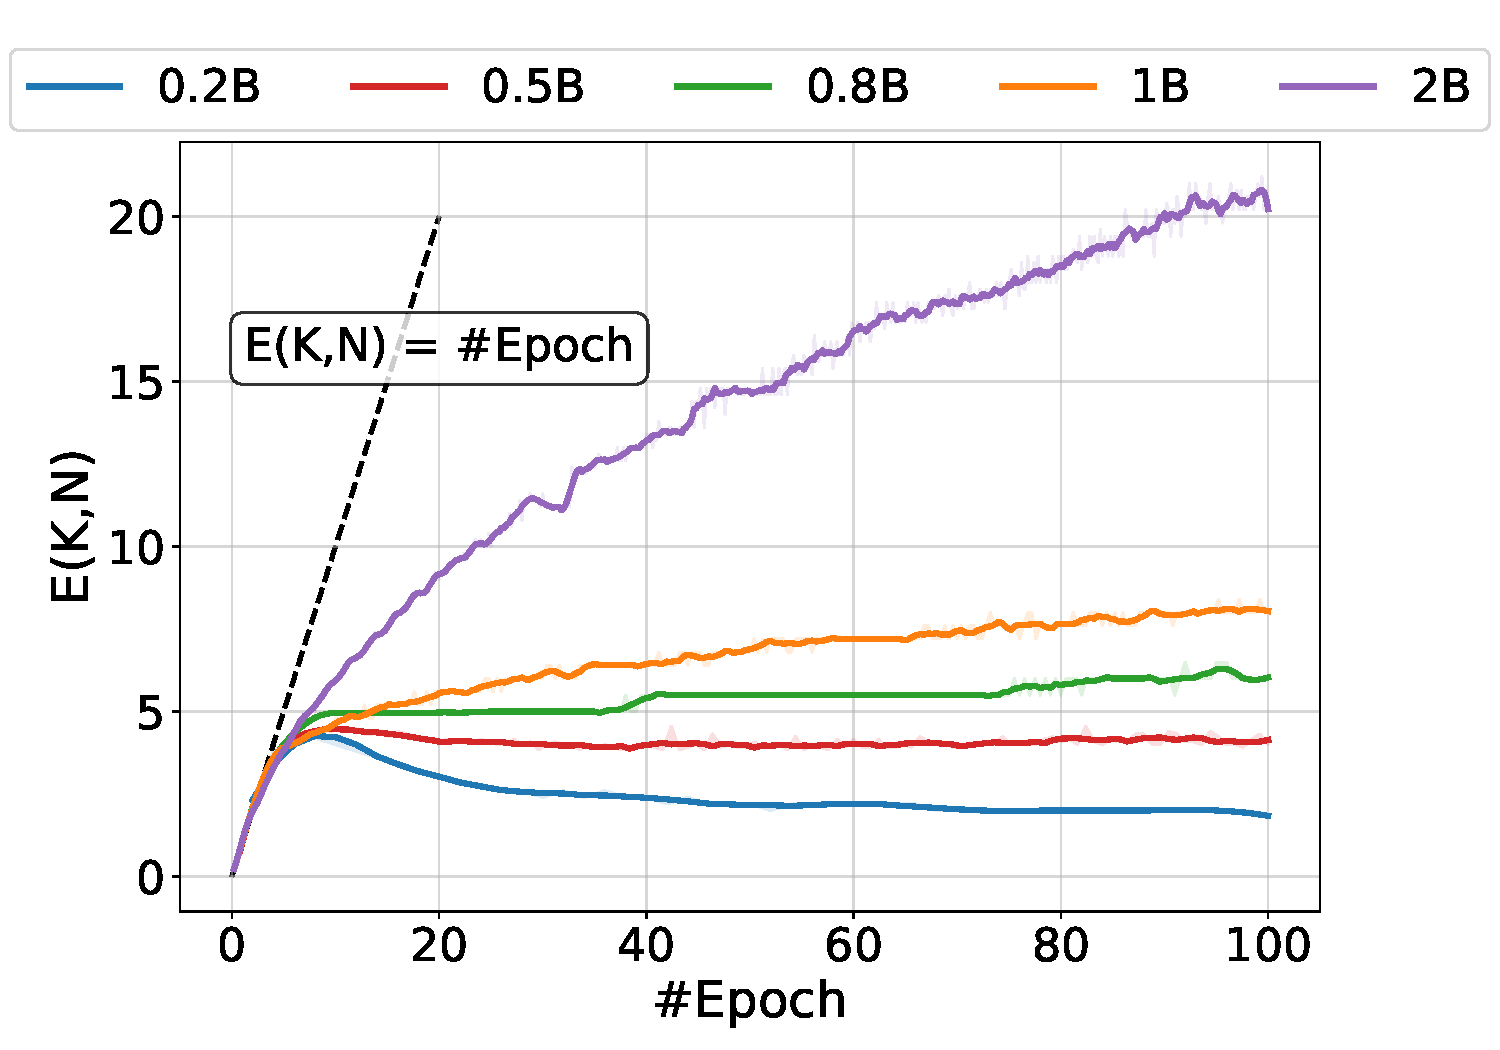
\includegraphics[width=0.48\linewidth]{figs/E_k_smoothed_shaded.pdf}
%     }\hfill
%     \subfigure[$E(K,N)$ v.s.~$N$.%
%       \label{fig:ek-data}]{
%         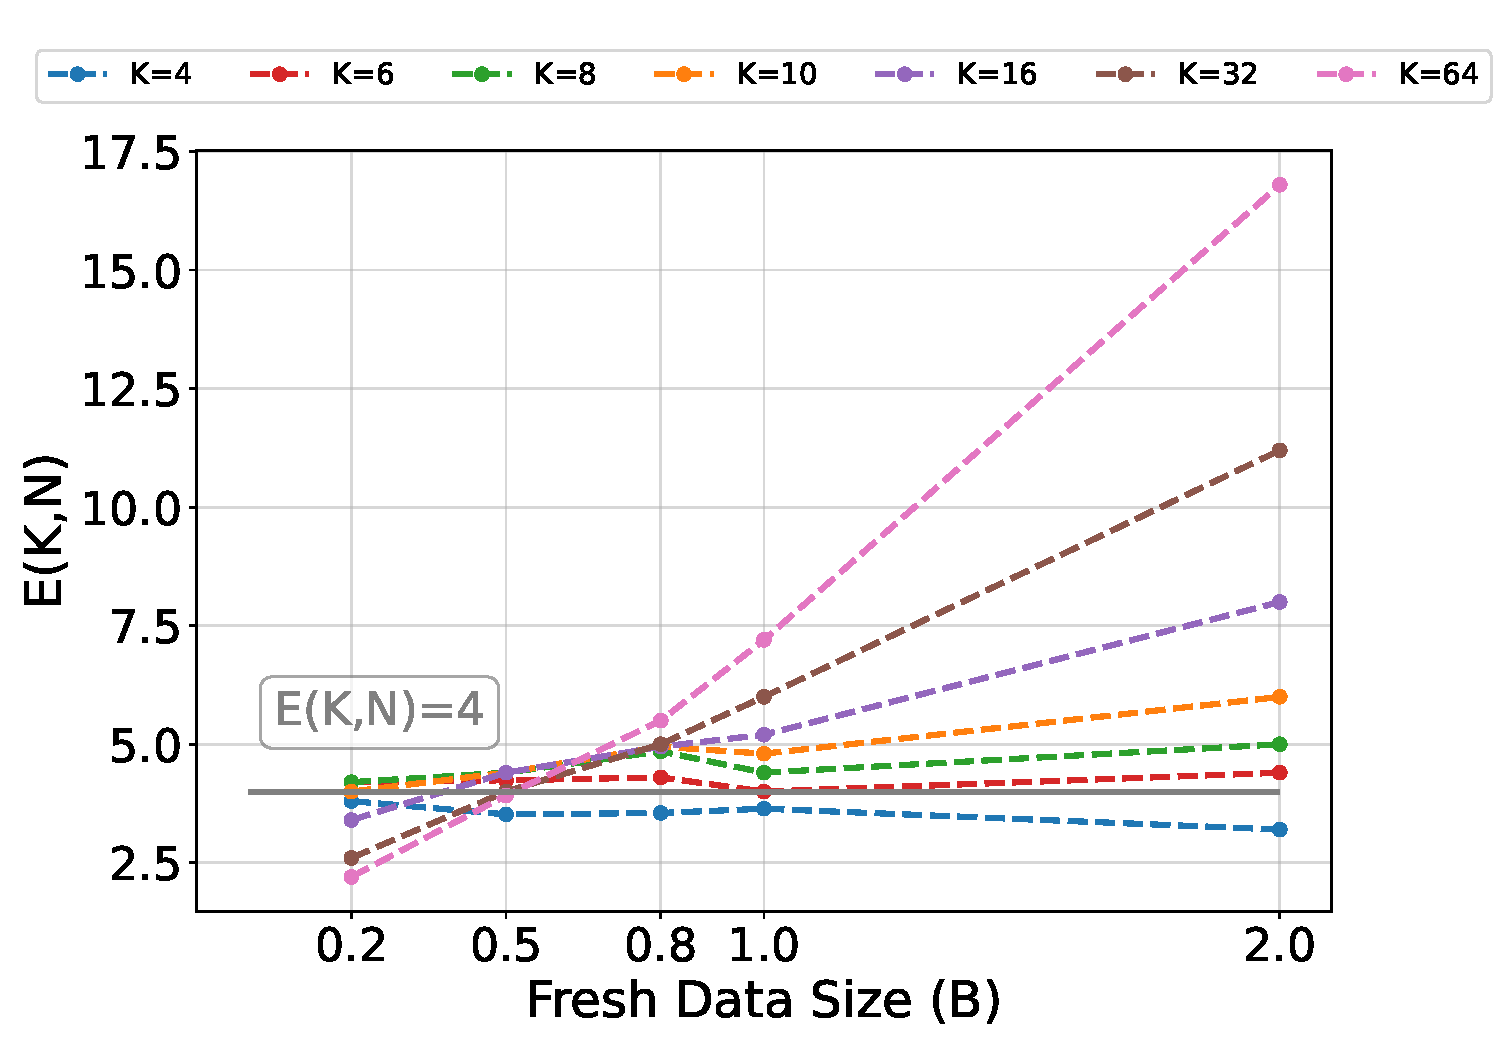
\includegraphics[width=0.48\linewidth]{figs/E_k_over_fresh_data_size.pdf}
%     }
%     \caption{In language model experiments, the effective reuse rate $E(K,N)$ behaves as follows:
%     (1) With $N$ fixed, $E(K,N)$ grows with $K$ before saturating at a value that increases with $N$;
%     (2) With $K$ fixed, $E(K,N)$ grows with $N$ and saturates at $K$.}
% \end{figure}

% \haodong{fix the definition of excess risk}
%Consider a linear regression problem with population loss $\cL(\vw) = \frac{1}{2} \E[(\langle \vw,\;\vx \rangle - y^*)^2]$, where $\vw \in \R^d$ represents the trainable parameter, $y^* = \langle \vw^*, \vx\rangle$, $\E\vx\vx^{\top}=\mH$, and $\vw^*$ is the ground truth.
\paragraph{Multi-Epoch SGD Training Algorithm.} Consider a finite training dataset with $N$ data points $\{(\vx_0,y_0),(\vx_1,y_1),\dots,(\vx_{N-1},y_{N-1})\}$, where the data points $(\vx_i, y_i)$ are i.i.d.~sampled from the distribution $\mathcal{D}$. We use $K$-epoch stochastic gradient descent (SGD) with random shuffling to minimize the loss function. And the initial parameter $\vw_0$ is set to $0$. Formally, we denote $K$ independent random permutations of $[N]$ by $\pi_1, \dots, \pi_K$. And we define $j_t := \pi_{k_t}(i_t)$, where $i_t := t \bmod N$, $k_t := \lfloor t / N \rfloor + 1$. Then we have the update rule for $K$-epoch SGD with $N$ data points
% \begin{align*}
%     \vw_{t+1} &= \vw_{t} - \eta \nabla_{\vw}\ell(\vw_t; \vx_{j_t}, y_{j_t}) \\
%     &=\left(\mI-\eta\vx_{j_t}\vx_{j_t}^{\top}\right)\vw_t+\eta\xi_{j_t}\vx_{j_t}.
% \end{align*}
\begin{equation}
    \vw_{t+1} = \vw_{t} - \eta \nabla_{\vw}\ell(\vw_t; \vx_{j_t}, y_{j_t}) =\left(\mI-\eta\vx_{j_t}\vx_{j_t}^{\top}\right)\vw_t+\eta\xi_{j_t}\vx_{j_t}. \nonumber
\end{equation}
Next, given a $K$-epoch SGD over $N$ data points, with learning rate $\eta$, we define $\cW_{K,N,\eta}$ to be the distribution of $\vw_{KN}$. The randomness within $\vw_{KN}$ comes from the random draw of the dataset, label noise $\xi$, and the shuffling in SGD. Based on this, we define the expected excess risk of a given $K$-epoch SGD over $N$ data points, with learning rate $\eta$ as $\bar{\cR}(K, N; \eta) := \E_{\vw \sim \cW_{K,N,\eta}}[\cR(\vw)]$. We assume $\eta \leq D^{-2}$ for training stability.

We also consider multi-epoch training under more practical training configurations, for example, using a class of polynomially decaying learning-rate schedules. See \Cref{app:discussion} for more details.
% \kaifengclaw{Typo/style: 'multi epoch' -> 'multi-epoch'; 'a polynomial decaying learning rate schedule class' can be simplified to 'a class of polynomially decaying learning-rate schedules'.}
% where $\eta$ is the learning rate, and $\pi_k$ denotes the permutation mapping in the $k$-th epoch that sends the i-th data to index $\pi_k(i)$. We assume $\eta < D^{-2}$ for training stability.
% \kaifeng{noise can cause oscillation too}

\begin{comment}
-----------

Given training time $t\in[(k-1)N, kN)$ for some $k\in\mathbb{N^*}$, we define $i_t:= t - (k-1)N \in [0, N-1]$.

$\vw_{k,i} $

$i_t = t \bmod N$

We define an alternative notation for $\vw_t$ as $\vw_{k, i+1}$, where $k$ represents the number of completed epochs and $i+1$ denotes the additional data points processed in the current epoch. Then the $t+1$-th iteration is given by
\begin{align*}
    \vw_{t+1} &= \vw_{t} - \eta \nabla_{\vw}\ell_{\vw_{t}}(\vx_{\pi_k(i)}, y_{\pi_k(i)}) \\
    &=\left(\mI-\eta\vx_{\pi_k(i)}\vx_{\pi_k(i)}^{\top}\right)\vw_t+\eta\xi_{\pi_k(i)}\vx_{\pi_k(i)},
\end{align*}
where $\eta$ is the learning rate, and $\pi_k$ denotes the permutation mapping in the $k$-th epoch that sends the i-th data to index $\pi_k(i)$. 
We assume $\eta < D^{-2}$ to avoid oscillation.\kaifeng{noise can cause oscillation too}


$\cW_{K,N}(\eta)$: the distribution of $\vw_{KN}$, where $\vw_{KN}$ is the weight at the last iteration of $K$-epoch SGD with data size $N$. The randomness comes from the random draw of the dataset and the shuffling in SGD

$\vw_{k,s} = \vw_{kN+s}$


With learning rate $\eta$, we denote the parameter updated by one-pass SGD at step $T$ by $\vw_T(\eta)$, and we the parameter updated by multi-epoch SGD at $k$-th epoch with dataset size $N$ is denoted by $\vw_{K,N}(\eta)$. When causing no confusion, we omit $(\eta)$ and denote them by $\vw_T$ and $\vw_{K,N}$ for short.
% from index $i$  to the corresponding index in the training dataset. 
\end{comment}

\paragraph{Comparing Performance under Optimal Learning Rate Regime.} %The learning rate plays a critical role in shaping the training dynamics of linear regression under SGD. Therefore, to enable a fair and meaningful comparison between one-pass and multi-epoch SGD, careful tuning of the learning rate is essential. 
To compare the performance of one-pass and multi-epoch SGD, we consider the settings where the learning rates for both methods are optimally tuned.
% tuned to the optimal.
% \kaifengclaw{Clarity: 'tuned to the optimal' sounds awkward; suggest 'optimally tuned' or 'tuned to their respective optima'.}
Formally, we introduce the notion of the \textit{optimal expected excess risk} of $K$-epoch SGD for $N$ samples as $\bar{\cR}^*(K, N):=\min_{\eta \in (0, \frac{1}{D^2}]}\{ \bar{\cR}(K, N; \eta) \}$. To calculate this value analytically, in the next section, we will show that we can get a learning rate choice that can approximately achieve the above optimal expected excess risk $\bar{\cR}^*(K, N)$ both for one-pass and multi-epoch SGD.
% \kaifengclaw{Typo/clarity: 'in math' -> 'analytically'; this sentence is long and repetitive ('we will show... we can get... can approximately achieve'). Consider splitting into two shorter sentences.}
Following our discussion in the introduction, we define the \textit{effective reuse rate} as follows:
\begin{definition}[Effective Reuse Rate]\label{def:E_K}
Given $K$-epoch SGD trained with $N$ fresh data samples, the effective reuse rate is defined as: $E(K,N) := \frac{1}{N}\min\{N' \ge 0: \bar{\cR}^*(1, N') \leq\bar{\cR}^*(K, N)\}$.
%%%$\kaifengclaw{Math-check: since $N'$ is a sample size, should the minimization domain be integers ($N'\in\mathbb{N}$)? If treated continuously for asymptotics, consider stating this explicitly to avoid ambiguity in derivations.}\kaifeng{no. it is clear that $N'$ is an integer.}
% \kaifengclaw{Consistency: earlier/later you use 'effective reuse rate'; here it says 'ratio'. Better keep one term consistently throughout.}
%\begin{equation}
%    E_{\eta, \eta'}(K,N) := \frac{1}{N}\min\{T' : \E[\cR(\vw_{T'}(\eta'))] \leq \E[\cR(\vw_{K,N}(\eta))]\}. \nonumber
%\end{equation}
% \begin{equation}
%     E_{\eta, \eta'}(K,N) := \frac{1}{N}\min\{T' : \bar{\cR}(1, T'; \eta') \leq \bar{\cR}(K, N; \eta)\}. \nonumber
% \end{equation}
% \begin{equation}
%     E(K,N) := \frac{1}{N}\min\{N' \ge 0: \bar{\cR}^*(1, N') \leq\bar{\cR}^*(K, N)\}. \nonumber
% \end{equation}
% \tingkai{Explanations}
% where $\bar{\cR}^*(K, N)$ denotes the optimal excess risk of $K$-epoch SGD trained with $N$ fresh data samples. Specifically $\bar{\cR}^*(1, N')$ denotes the optimal excess risk of one-pass SGD with steps $N'$.
\end{definition}

\vspace{-0.05in}
That is, the effective reuse rate measures how many times larger the dataset must grow under one-pass training to match the performance of $K$-epoch training, both under the optimal learning rate regime.


%This definition characterizes the equivalent number of epochs required for OP SGD with the optimal learning rate, corresponding to the optimal expected excess risk of ME SGD. This definition characterizes the effectiveness of scaling in data reusing regime.
%To study the scaling behavior of data reusing, 

%we first tune the learning rate of one-pass (OP) SGD to be as close to optimal as possible, thereby establishing a baseline for comparison. Subsequently, we design an approximately optimal learning rate for multi-epoch (ME) SGD and compare its performance with that of the other methods. However, precisely determining the optimal learning rate for both OP and ME SGD remains challenging. To address this, 

% \[
%     \bar{\cR}^*(K, N):=\min_{\eta \in (0, \frac{1}{D^2}]}\{ \bar{\cR}(K, N; \eta) \}.
% \]
%$\eta^* = \eta^*(K,N) = \arg\min_{\eta \in (0, \frac{1}{D^2})}\E\left[\cR\left(\vw_{K,N}(\eta)\right)\right]$. 

% optimal excess risk of $K$-epoch SGD for $N$ samples: $\bar{\cR}^*(K, N):=
% \min_{\eta \in (0, \frac{1}{D^2})}\{ \bar{\cR}(K, N; \eta) \}$.

%$\eta^*(K,N) \in \argmin_{\eta \in (0, \frac{1}{D^2})}\{ \bar{\cR}(K, N; \eta) \}$. We choose an arbitrary 

%\E\left[\cR\left(\vw_{K,N}(\eta^*)\right)\right]$.

% Also, we can denote that the minimal excess risk achieved by the optimal learning rate $\E[\cR^*(\vw_{K,N})] :=\E[\cR^*(\vw_{K,N}(\eta^*))]$. Then we show in the next section that we can get an alternative learning rate choice that can approximately achieve the minimal excess risk of the optimal learning rate $\eta^*$.
% \haodong{definition not even clear}
%maybe we don't need this def
% \begin{definition}[Optimal Learning Rate]\label{def:opt-lr}
%     We define the optimal learning rate with completed training epochs $K$ and dataset size $N$ as
%     \begin{align*}
%         \eta^* = \eta^*(T) = \arg\min_{\eta \in (0, \frac{1}{D^2})}\E\left[\cR\left(\vw_{K,N}(\eta)\right)\right].
%     \end{align*}
% \end{definition}
% Futher, we can denote that the minimal excess risk achieved by the optimal learning rate $\E[\cR^*(\vw_{K,N})] :=\E[\cR^*(\vw_{K,N}(\eta^*))]$.

% \begin{definition}[Approximate Expected Population Excess Risk]\label{def:A-loss}
%     We say that a function $\widehat{\cR}:\mathbb{N}\times\mathbb{R}\rightarrow\mathbb{R}$ is an approximate population excess risk at iteration $T$ within a range $[f(T), g(T)]$ for two functions $f(T), g(T) = o_T(1)$ that satisfies $\eta^* \in [f(T), g(T)]$, if $\E[\cR(\vw_T(\eta))] = \widehat{\cR}(T, \eta)(1+o_T(1))$ holds for all learning rates $\eta \in [f(T), g(T)]$. 
% \end{definition}

% Based on the above approximate population excess risk, we define the following approximately optimal learning rate.

% \begin{definition}[Approximately Optimal Learning Rate]\label{def:A-opt-lr}
% %     For a given total training time $T$, we define the approximately optimal learning rate set as follows:
% % \begin{equation}
% %     \Gamma_{T}:=\{\eta^*: \exists \text{ an approximate population excess risk }\widehat{\cR} \text{ s.t. } \eta^*\in \operatorname{\arg \min}_{\eta} \widehat{\cR}(T, \eta) \}. \nonumber
% % \end{equation}
% % \kairong{I guess here $\Gamma_T$ is actually $\Gamma_T(\widehat{\cR})$}

% % For the expected loss estimate $\E[\cL(\vw_T)] = \fakeE[\cL(\vw_T)](1 + o(1))$, then we define the set of asymptotic optimal learning rates $\Gamma_{A-opt}$ is the set  such that
% % \begin{align*}
% %     \Gamma_{A-opt} := \{\eta_*: \eta_* = \arg \min_{\eta} \fakeE[\cL(\vw_T)]\}.
% % \end{align*}
% \end{definition}
%\vspace{-0.75em}
%\paragraph{Effective Reuse Rate.}
% \haodong{I think we need one sentence more for the transition from the choice of learning rate to $E_K(K,N)$} 
%Now, we formally introduce the key concept in our paper as follows:
% \haodong{also we need some interpretation for this definition here}
%     Given $K$-epoch SGD with some learning rate $\eta_{\ME} = f(K,N)$, whose expected loss after $T=KN$ steps is denoted by $\E[\cL_{\ME}(\vw_{KN})]$ and one-pass SGD with learning rate $\eta_{\OP} = g(T')$, whose expected loss after $T'$ is denoted by $\E[\cL_{\OP}(\vw_{T'})]$, we define the effective number of epochs as
%     \begin{align*}
%         E_K = \frac{1}{N}\min\{T':\E[\cL_{\OP}(\vw_{T'})]  \le \E[\cL_{\ME}(\vw_{KN})]\},
% \end{align*}
% where $f(\cdot,\cdot):\R^+\times\R^+\to\R^+$, and $g(\cdot):\R^+\to\R^+$


\section{Multi-Epoch Scaling in Strongly Convex Linear Regression}
\label{sec:strongly_convex}
In the study of linear regression problems, the strongly convex case is a classical and central theoretical framework, serving as the standard entry point before relaxing to weaker conditions in many analyses~\citep{hastie2009elements,ge2019step}.
% \kaifengclaw{Grammar: 'before many relaxing' -> 'before relaxing to weaker conditions in many analyses' (or similar).} 
In \Cref{sec: main results strongly convex}, we first give the problem setups and the main results of the effective reuse rate. In \Cref{sec:strongly-convex-tech}, we give a proof sketch for our theoretical results, and the detailed proof of this section can be found in Appendix~\ref{sec:proof-convex}. 
% In this section, we first present our main results about multi-epoch (ME) scaling under the strongly convex condition. And in \Cref{sec:strongly-convex-tech}, we present the key technical challenges in the proof, including the excess risk approximation, and the optimal learning rate for OP and ME, and the derivation of $E(K,N)$. Also, we provide a population excess risk approximation theorem (\Cref{thm:convex-L-estimate}) as a byproduct. The detailed proof of the main results in this section can be found in \Cref{sec:proof-convex}. \haodong{rephrase this paragraph since we rewrote the proof sketch}

\vspace{-0.07in}
\subsection{Main Results}\label{sec: main results strongly convex}

As we focus on the strongly convex case, we make the following assumption on the minimum eigenvalue of the Hessian matrix.
\begin{assumption}[Strong Convexity]\label{asp:strongly-convex}
    We assume that $\lambda_{d} \ge \mu\;$ for some constant $\mu > 0$.
\end{assumption}
% \haodong{$c \to \mu$}
%\Cref{asp:4-th-moment} is the Assumption 3.2 in \citep{wu2022iterateriskboundssgd}.
% \begin{assumption}[Hyper-Contractivity]\label{asp:4-th-moment}
% We assume that there exists $\alpha \geq 1$ such that for every positive semi-definite matrix $\mP$, the following holds:
% $$
% \mathbb{E}\left[\vx \vx^\top \mP \vx \vx^\top \right] \leq \alpha \, \text{tr}(\mH \mP) \mH.
% $$
% \end{assumption}
% \haodong{the above assumption can be derived from bounded data norm}

\vspace{-0.05in}
For simplicity, we make the following prior for the ground-truth weight $\vw^*$.
\begin{assumption}[Parameter Prior] \label{asp:strongly-convex-parameter-prior}
    The ground truth $\vw^*$ satisfies $w^*_i \ne 0$ for all $i\in[d]$.
\end{assumption}
% \haodong{explanation of the assumption. }

\vspace{-0.05in}
As the number of samples $N$ can be very large in practice, training on the entire dataset for a large amount of epochs can be computationally expensive.
This motivates us to impose an upper bound on the number of epochs $K$. Technically, this ensures that the accumulated error terms remain manageable in our analysis.
% Technically, this helps us to rule out cases with severe overfitting. \kaifeng{I remember that the last sentence is not true. How about this: Technically, this ensures that the accumulated error terms remain manageable in our analysis.}
\begin{assumption}[Computationally feasible number of epochs]\label{asp:large-dataset}
We assume that the training dataset size $N$ and number of epochs $K$ satisfy $K = O(N^{0.1})$.
\end{assumption}

\vspace{-0.05in}
Here, the exponent $0.1$ is chosen for ease of calculation, though it may not be tight.


%For ease of calculation, we make this assumption.
%Though the exponent $0.1$ may not be tight, one can tighten it easily. Empirically, the limited reusing epochs also prevent over-fitting.

% \haodong{specify the exponent of poly function; for ease of calculation, we make this assumption, though it may not be tight}
% \begin{lemma}\label{thm:convex-opt-lr}
%     Under \Cref{asp:strongly-convex}, \ref{asp:4-th-moment}, and \ref{asp:large-dataset}, we consider one-pass SGD with $T$ steps and learning rate $\eta$ satisfying $\eta = o(T^{-3/4})$ and $\eta = \Omega\left(\frac{1}{T}\right)$. Then the approximately optimal learning rate set contains $\frac{\log T}{2 \lambda_d T} + o\left(\frac{\log T}{T}\right) \in \Gamma_{T}$, where $\Gamma_{T}$ is the approximately optimal learning rate set defined in \Cref{def:A-opt-lr}. \kairong{For all $\widehat{\cR}$, this Lemma holds?}
% \end{lemma}

% \begin{remark}
%     The derivation of the optimal learning rate is very hard, and this open problem is quite beyond the scope of this paper, which focuses on the scaling behaviour of deta reuse. As an alternative choice, we could get an asymptotically optimal learning rate as \Cref{thm:convex-opt-lr} stated.
% \end{remark}
% Obtaining the expression of $E(K, N)$ requires an accurate characterization of the optimal expected excess risk. Here we provide an expression of $\Bar{\cR}^*(K, N)$ when $K=o(\log N)$ and $K=\Omega(\log N)$ in the formulation of the main term plus a higher-order error term.

To compute $E(K,N)$, we first precisely characterize the optimal expected excess risk. 
In particular, we derive asymptotic expansions for $\Bar{\cR}^*(K,N)$ in the regimes $K=o(\log N)$ and $K=\omega(\log N)$, each expressed as a leading term accompanied by an explicitly controlled higher\mbox{-}order remainder.

\begin{theorem}[Multi-Epoch Data  Scaling Law]\label{thm:strongly-convex-scaling-law}
    Under \Cref{asp:strongly-convex,asp:strongly-convex-parameter-prior,asp:large-dataset}, for multi-epoch SGD with the number of epochs $K$, dataset size of $N$, it holds that
\[
\Bar{\cR}^*(K,N) = 
\begin{cases}
     \frac{\sigma^2\tr(\mH)}{8\lambda_d}(1+o_N(1)) \cdot \frac{\log(KN)}{KN} & \text{for } K = o(\log N), \\
     \frac{\sigma^2d}{2}(1+o_N(1)) \cdot \frac{1}{N} & \text{for } K = \omega(\log N).
\end{cases}
\]
\end{theorem}

\vspace{-0.1in}
\Cref{thm:strongly-convex-scaling-law} describes how expected excess risk decays with number of epochs $K$ and dataset size $N$ when choosing the optimal learning rate. When $K\ll \log N$, then $\Bar{\cR}^*(K,N) =\Theta\left(\frac{\log T}{T}\right)$ where $T = KN$; by contrast, when $K\gg \log N$, then $\Bar{\cR}^*(K,N) =\Theta\left(\frac{1}{N}\right)$ which does not depend on $K$, showing that endless data reuse turns out to be useless.
% \kaifengclaw{Typo: 'turns to be' -> 'turns out to be'.}

Next we propose the expression of $E(K,N)$ by applying \Cref{thm:strongly-convex-scaling-law}.
\begin{theorem}\label{thm:convex-E_K}
    Under \Cref{asp:strongly-convex,asp:strongly-convex-parameter-prior,asp:large-dataset}, for multi-epoch SGD with the number of epochs $K$, dataset size of $N$, it holds that
\[
E(K,N) = 
\begin{cases}
     (1 + o_N(1))\cdot K & \text{for } K = o(\log N), \\
     \frac{\tr(\mH)}{4\lambda_d d}(1+o_N(1)) \cdot \log N & \text{for } K = \omega(\log N).
\end{cases}
\]
\end{theorem}
% \tingkai{I determined the constant here, and changed the comment below.}

%\haodong{the following 4 paragraphs can be shortened}

\vspace{-0.1in}
\Cref{thm:convex-E_K} pinpoints two regimes for the effective reuse rate in the strongly convex case. 
The first one is the \textbf{effective‐reuse regime}: when $K \ll \log N$, then $E(K,N)=K\,(1+ o(1))$. This suggests that each extra epoch is essentially as valuable as a fresh pass. 
The second one is the \textbf{limited‐reuse regime}: when $K \gg \log N$, then $E(K,N)=\frac{\tr(\mH)\log N}{4\lambda_d d}(1+o_N(1))$, which means additional epochs yield only logarithmic gains. This further implies that the model has effectively “seen” the dataset enough times that additional repetition is redundant.
% Thus, 
% % there is a phase transition at $K = \Theta(\log N)$: below it, reuse is highly effective; above it, returns rapidly diminish. 
% % Practically, one could allocate at most $O(\log N)$ epochs to maximize data efficiency.
% \Cref{thm:convex-E_K} rigorously delineates two complementary scaling regimes for the effective reuse rate $E(K,N)$ in the strongly‐convex setting. When the number of passes $K$ is much smaller than the logarithm of the dataset size (i.e.\ $K \ll \log N$), the theorem guarantees $E(K,N)= K\bigl(1\pm o(1)\bigr)\,$, meaning that each additional epoch yields nearly the same benefit as a fresh pass over an entirely new batch of data.  Intuitively, in this \emph{effective‐reuse regime}, the gradient noise induced by stochastic sampling is still large enough that revisiting past examples continues to drive significant progress.

% By contrast, once $K$ grows beyond the threshold $\log N$ (i.e.\ $K \gg \log N$), \Cref{thm:convex-E_K} shows $E(K,N)=\Theta\bigl(\log N\bigr)$, so that further epochs only increase the effective sample complexity by a logarithmic factor.  In this \emph{limited‐reuse regime}, the model has effectively “seen” the dataset enough times that additional repetition is redundant: the variance has been driven so low that further tuning behaves like running fresh SGD on a tiny virtual dataset of size $\Theta(N \log N)$.
% %\kairong{Very confusing. I guess here is a dataset of size $N\log N$.}

Together, these two asymptotic descriptions expose a phase transition when the quantity $\lim_{N \to \infty} \frac{K}{\log N}$ changes from $0$ to $\infty$.  For the former case ($\lim_{N \to \infty} \frac{K}{\log N} = 0$), multi‐epoch training behaves like unlimited data augmentation; for the latter ($\lim_{N \to \infty} \frac{K}{\log N} = \infty$),
% \kaifengclaw{Typo: 'fo the latter' -> 'for the latter'. Also this sentence is long; consider splitting at the semicolon for smoother logic transition.} 
the benefits of reusing data all but vanish, capping $E(K,N)$ at $\Theta(\log N)$.
%This insight provides a precise guideline for practitioners: one should allocate epochs up to order $\log N$ to maximize effective data utilization, but pushing $K$ significantly beyond that yields rapidly diminishing returns.

\paragraph{Larger Datasets Can Be Repeated More.} 
Our theorem provides the following insight.
Fixing the data distribution, as we collect more data, the largest possible epoch number $K$ to stay in the effective-reuse regime also increases.
%for larger datasets (as $N$ increases), the permissible $K$ value in the effective-reuse regime also increases.
Consequently, larger datasets can sustain more epochs while maintaining linear gains from data reuse.
%This means that for larger datasets, multi-epoch training is able to reuse every data point more effectively.
Specifically, for the setup we study in this section, if we have collected $N$ data points in total, then with multi-epoch training, we can get a performance comparable to one-pass training on $\Theta(N \log N)$ data points, which is superlinear in the number of data points we collected.
This finding highlights a neglected factor in the data-constrained scaling laws proposed in \citet{muennighoff2023scaling}, which assumed a uniform effective number of epochs across different fresh data sizes.
In~\Cref{sec:experiment-llm}, we validate this insight by showing that the effective reuse rate indeed increases with the dataset size in LLM pretraining.

\paragraph{Discussion: Effect of Learning Rate Decay.} The factor $\log N$ is in fact associated with the use of constant learning rate in our setting, where $\eta$ may depend on the total number of steps but remains fixed throughout training.
While our main focus is on the constant learning rate setting, introducing learning rate decay may lead to different scaling behaviors and warrants further theoretical investigation.
Under learning rate decay, for example using $\eta_t = \frac{\eta_0}{1 + b t^\alpha}$ with $b > 0$ and $0.5 < \alpha \le 1$ at step $t$, by a direct calculation based on the setup of Theorem 1 in \citet{ge2019step}, it is not hard to show that one-pass training yields $\Bar{\cR}^*(1,N) = O(\kappa_{\mH} \cdot \frac{\sigma^2 d}{N})$ for sufficiently large $N$ when $\alpha=1$, where $\kappa_{\mH} := \frac{\lambda_1}{\lambda_d}$ is the condition number of $\mH$. 
% (e.g., by following a similar calculation in~\citet{???}\kaifeng{cite something}). 
This bound loses only by a constant factor compared to the statistical minimax rate $\frac{\sigma^2 d}{2N}$ implied by the Cramér--Rao lower bound~\citep{jain2017markov}.
Therefore, under learning rate decay, the effective reuse rate of multi-epoch training is at most $O(\kappa_{\mH})$.
In~\Cref{app:discussion}, we provide a preliminary analysis comparing one-pass and multi-epoch training in the limit of infinitely many epochs, showing that multi-epoch training can almost attain the statistical minimax rate and achieve $E(\infty, N) = \Omega(\kappa_{\mH})$.
It remains an interesting direction to understand how $E(K, N)$ saturates to this value and how it depends on the dataset size $N$.

%A precise characterization for finite $K$ to understand 

%remains an interesting direction for future work.


%one-pass training yields $\Bar{\cR}^*(1,N) \le \frac{C D^2}{\lambda_d} \cdot \frac{\sigma^2 d}{N}$ for sufficiently large $N$ for some $C > 0$~\kaifeng{@Tingkai, is this bound correct? also cite something here}. 

%This bound loses only by a constant factor compared to the statistical minimax rate $\frac{\sigma^2 d}{2N}$ implied by the Cramér--Rao lower bound.\kaifeng{cite something}
%Therefore, under learning rate decay, the effective reuse rate of multi-epoch training is at most $O(1)$ rather than $O(\log N)$.
%While our main focus is on the constant learning rate setting, this different scaling behavior warrants further theoretical investigation.
%In~\Cref{app:discussion}, we provide a preliminary analysis comparing one-pass and multi-epoch training in the limit of infinitely many epochs, showing that multi-epoch training can almost attain the statistical minimax rate and achieve $E(\infty, N) > 1$.
%A precise characterization for finite $K$ remains an interesting direction for future work.


%observation is further validated in our experiments with large language models in \Cref{sec:experiment-llm}.
%As a byproduct, our results also provide theoretical counterexamples to the formula for $E(K,N)$ proposed in \citet{muennighoff2023scaling}, namely $E(K,N) = \left(1 + R^* (1 - e^{-(K-1)/R^*})\right)$, which suggests that $E(K,N)$ is independent of $N$.


% \haodong{the following 4 paragraphs can be shortened}

% \Cref{thm:convex-E_K} pinpoints two regimes for the effective reuse rate in the strongly convex case. 
% If $K \ll \log N$, then $E(K,N)=K\,(1+ o(1))$: each extra epoch is essentially as valuable as a fresh pass. 
% If $K \gg \log N$, then $E(K,N)=\frac{\tr(\mH)\log N}{4\lambda_d d}(1+o_N(1))$: additional epochs yield only logarithmic gains. 
% Thus, there is a phase transition at $K = \Theta(\log N)$: below it, reuse is highly effective; above it, returns rapidly diminish. 
% Practically, one could allocate at most $O(\log N)$ epochs to maximize data efficiency.

% \Cref{thm:convex-E_K} rigorously delineates two complementary scaling regimes for the effective reuse rate $E(K,N)$ in the strongly‐convex setting. When the number of passes $K$ is much smaller than the logarithm of the dataset size (i.e.\ $K \ll \log N$), the theorem guarantees $E(K,N)= K\bigl(1\pm o(1)\bigr)\,$, meaning that each additional epoch yields nearly the same benefit as a fresh pass over an entirely new batch of data.  Intuitively, in this \emph{effective‐reuse regime}, the gradient noise induced by stochastic sampling is still large enough that revisiting past examples continues to drive significant progress.

% By contrast, once $K$ grows beyond the threshold $\log N$ (i.e.\ $K \gg \log N$), \Cref{thm:convex-E_K} shows $E(K,N)=\Theta\bigl(\log N\bigr)$, so that further epochs only increase the effective sample complexity by a logarithmic factor.  In this \emph{limited‐reuse regime}, the model has effectively “seen” the dataset enough times that additional repetition is redundant: the variance has been driven so low that further tuning behaves like running fresh SGD on a tiny virtual dataset of size $\Theta(N \log N)$.
% %\kairong{Very confusing. I guess here is a dataset of size $N\log N$.}

% Together, these two asymptotic descriptions expose a phase transition around $K \approx \log N$.  Below this threshold, multi‐epoch training behaves like unlimited data augmentation; above it, the benefits of reusing data all but vanish, capping $E(K,N)$ at $\Theta(\log N)$.  This insight provides a precise guideline for practitioners: one should allocate epochs up to order $\log N$ to maximize effective data utilization, but pushing $K$ significantly beyond that yields rapidly diminishing returns.

% \paragraph{Larger Datasets Can Be Repeated More.} Also, we have provided a new insight in the calculation in the above theorem. Specifically, for larger datasets (as $N$ increases), the permissible $K$ value in the effective-reuse regime also increases. This means that for larger datasets, a higher degree of data reuse is allowed. This observation is further validated in our experiments with large language models in \Cref{sec:experiment-llm}.

% As a side product, our results also theoretically provide counterexamples for the proposed formula for $E(K,N)$ in \citet{muennighoff2023scaling}, as shown in \Cref{equ:data-constrained-EK}, which inferred that $E(K,N)$ is independent of $N$.

\vspace{-0.07in}
\subsection{Proof Sketch}\label{sec:strongly-convex-tech}

\vspace{-0.03in}
We now provide a proof sketch of our main results. 
First, we need to compute the optimal expected excess risk $\bar{\cR}^*(K,N)$. This requires us to compute $\bar{\cR}(K,N;\eta)$ and then select the optimal learning rate $\eta^*$ that minimizes $\bar{\cR}(K,N;\eta)$. However, due to the random shuffling and multi-pass processing of the training data, directly analyzing $\bar{\cR}(K,N;\eta)$ is intractable. To overcome this, we seek an analytic approximation of $\bar{\cR}(K,N;\eta)$, which is derived through the following steps.

\paragraph{Step 1: Bias-Variance Decomposition for Training Dynamics.} \label{step:bias-var-decomposition} 
Following the widely-applied bias-variance decomposition approach to analyzing the dynamics of SGD training~\citep{neu2018iterate, ge2019step, zou2021benign, wu2022iterateriskboundssgd}, we define $\vtheta_t = \vw_t - \vw^*$ and examine the following two processes of bias and variance: $\vtheta_{t+1}^{\bias} = \vtheta_t^{\bias} - \eta \inp{\vtheta_t^{\bias}}{\vx_{j_t}}\vx_{j_t}, \vtheta_{t+1}^{\var} = \vtheta_t^{\var} - \eta \inp{\vtheta_t^{\var}}{\vx_{j_t}}\vx_{j_t} + \eta \xi_{j_t}\vx_{j_t}$,
% \begin{equation}
%     \vtheta_{t+1}^{\bias} = \vtheta_t^{\bias} - \eta \inp{\vtheta_t^{\bias}}{\vx_{j_t}}\vx_{j_t}, \quad \vtheta_{t+1}^{\var} = \vtheta_t^{\var} - \eta \inp{\vtheta_t^{\var}}{\vx_{j_t}}\vx_{j_t} + \eta \xi_{j_t}\vx_{j_t} , \nonumber
% \end{equation}
where the two processes are initialized as $\vtheta_0^{\bias} = \vw_0 - \vw^*$ and $\vtheta_0^{\var} = \boldsymbol{0}$.
% \kaifengclaw{Grammar: add article -> 'where the two processes are initialized as ...'.} 
It follows that $\vtheta_t = \vtheta_t^{\bias} + \vtheta_t^{\var}$, with $\E[\vtheta_t^{\text{var}}] = \boldsymbol{0}$. We can then decompose the excess risk $\cR(\vw_t)$ into two components: the \textit{bias term} and the \textit{variance term}, which we formalize as follows $\cR(\vw_t) = \frac{1}{2}\left\|\vtheta_{t}\right\|_{\mH}^2 =  \frac{1}{2}\left\|\vtheta_t^{\bias}\right\|_{\mH}^2 + \frac{1}{2}\left\|\vtheta_t^{\var}\right\|_{\mH}^2.$
% \begin{align}
%     \cR(\vw_t) = \frac{1}{2}\left\|\vtheta_{t}\right\|_{\mH}^2 =  \frac{1}{2}\left\|\vtheta_t^{\bias}\right\|_{\mH}^2 + \frac{1}{2}\left\|\vtheta_t^{\var}\right\|_{\mH}^2.\label{equ:bias-var-decomposition} 
% \end{align}

\paragraph{Step 2: Analytic Risk Approximation by Matrix Concentration.} A key challenge in tracking the dynamics of multi-epoch SGD training arises from the non-commutative nature of the matrices in the weight updates, which depend on randomly shuffled and multi-pass data. 
For example, the bias weight evolves as
$\vtheta_{KN}^{\bias} = \left(\prod_{k=1}^{K} \left(\prod_{l=1}^{N} \left(\mI-\eta \vx_{\pi_k(l)}\vx_{\pi_k(l)}^{\top}\right)\right)\right) \vtheta_{0}^{\bias},$
%\haodong{in multi epoch one data point appears more than once across different epochs -> the data is correlated in a long matrix multipulication -> thus calculating the expectation is intractable} 
where we can see that one data point appears more than once across different epochs. Thus, the above matrix multiplication involves massive correlated data, which makes calculating the bias term $\E\left[\left\|\vtheta_{KN}^{\bias}\right\|_{\mH}^2\right]$ intractable.
% Due to the non-commutativity of matrix multiplication, computing the expectation of the bias term $\E\left[\left\|\vtheta_{KN}^{\bias}\right\|_{\mH}^2\right]$ is intractable. 
To resolve this issue, we borrow tools from concentration inequalities for matrix products~\citet{huang2022matrix}. Specifically, we use the following result:
\begin{lemma}[Corollary of Theorem 7.1 in \citet{huang2022matrix}]
\label{lem:un-shuffle-A-EA-expectation-main}
    Given $n$ data points such that $\vz_0, \cdots \vz_{n-1} \overset{i.i.d}{\sim} \cN(0, \mH)$, and defining $\mA = \prod_{j=0}^{n-1}\left(\mI-\eta \vz_{j}\vz_{j}^{\top}\right)$, we have
    $\E\|\mA-\E\mA\|^l \leq \left(\sqrt{\deltaA\eta^2nl}\right)^l,$
    where $\deltaA:= \Tilde{C}8eD^4\log d$ for some absolute constant $\Tilde{C} > 0$.
\end{lemma}
% \haodong{how to apply Lemma 4.1 to get the error bound analysis.}
However, several obstacles prevent us from directly applying \Cref{lem:un-shuffle-A-EA-expectation-main} to our problem. For example, we actually need to control error terms like $\E\left\|\prod_{i=K}^{k+1}\mA^{(i)} - (\mathbb{E}\mA)^l \right\|$, where $\mA^{(i)}$ represents the product of sequential updates through all samples in epoch $i$ (see the formal definition in \Cref{app:A_def}, Appendix~\ref{app:notation}). To address this, our main idea is to derive a tight upper bound for the original term, and decompose this upper bound into the sum of a series of sub-terms for which we can apply \Cref{lem:un-shuffle-A-EA-expectation-main}. (see the detailed derivation in Appendix~\ref{app:var-term-proof} and Appendix~\ref{app:bias-proof})
% such that any two $\mA^{(i)}$ are correlated with each other, thus we cannot directly apply \Cref{lem:un-shuffle-A-EA-expectation-main} to our problem. Our method to deal with this issue is summarized as follows: (1) we represent each $\mA^{(i)}$ as the sum of the main term and the error term, and (2) we rewrite the error term into a sum of matrix products, then (3) we apply Cauchy-Schwarz inequality to split each product into independent terms. 

Finally, we derive an error bound on matrix deviations based on our calculations, which is a higher-order infinitesimal of the main term when $\eta \in \left[\Omega\left(T^{-1}\right), o(T^{-\frac{3}{4}})\right]$ and $K = o\left(\eta^{-1} T^{-\frac{3}{4}}\right)$, with $T:=KN$ denoting the total number of training steps. This provides a theoretical guarantee for us to approximate the risk function with a tractable expression. For the bias term, we have
\begin{align*}
    \E\left[\left\|\vtheta_{KN}^{\bias}\right\|_{\mH}^2\right]
    &= \E\left[\left\|\left(\prod_{k=1}^{K} \left(\prod_{l=0}^{N-1} \left(\mI-\eta \vx_{\pi_k(l)}\vx_{\pi_k(l)}^{\top}\right)\right)\right)\vtheta_0\right\|_{\mH}^2\right] \\
    &\approx \left\|\left(\prod_{k=1}^{K} \E\left[\prod_{l=0}^{N-1} \left(\mI-\eta \vx_{\pi_k(l)}\vx_{\pi_k(l)}^{\top}\right)\right]\right)\vtheta_0\right\|_{\mH}^2 \\
    &=\left\|\left((\mI-\eta\mH)^{KN}\right)\vtheta_0\right\|_{\mH}^2,
\end{align*}
where the approximation step follows from \Cref{lem:un-shuffle-A-EA-expectation-main}, and the last equation follows the facts that $\E\left[\vx_{\pi_k(l)}\vx_{\pi_k(l)}^{\top}\right] = \mH$ and $\vx_i$ is uncorrelated with $\vx_j$ for $i \neq j$.
% \kaifengclaw{Readability breakpoint: this proof-sketch step compresses the passage from products of random matrices to products of expectations. A short pointer to the exact decoupling identity used in Appendix (or one intermediate displayed line) would help readers see why the approximation error remains controlled under shuffling.}
%%%\kaifengclaw{Math-check: this step effectively exchanges expectation and non-commutative matrix products; 'uncorrelated' may be insufficient for product-factorization under random shuffling. Suggest explicitly stating the exact lemma/independence argument used for this equality to avoid a potential derivation gap.} \kaifeng{no, this is just a proof sketch}
For the variance term, the data correlation issue is similar to what we met in the bias term case. Again, leveraging \Cref{lem:un-shuffle-A-EA-expectation-main} and following a similar analysis, we can get an approximation formula for the variance term as shown:
\begin{align*}
        \E\left[\left\|\vtheta_{KN}^{\var}\right\|_{\mH}^2\right]&\approx\frac{2\sigma^2}{N} tr\left(\frac{\left(\mI -(\mI -\eta\mH)^{KN}\right)\left((\mI -\eta\mH)^{N} -(\mI -\eta\mH)^{KN}\right)}{\mI + (\mI -\eta\mH)^N}\right)\\
    &~~~~+{\eta\sigma^2}\inp{\mH}{(\mI - (\mI - \eta \mH)^{2KN})(2\mI-\eta\mH)^{-1}}.
\end{align*}

\paragraph{Step 3: Narrowing the Range for Optimal Learning Rate.}
However, although we have an analytic approximation for risk, it is important to note that this approximation holds only for a specific range of parameters.
% \kaifengclaw{Grammar: 'despite we have' -> 'although we have' or 'despite having'.} 
For a detailed discussion, refer to Lemma~\ref{thm:convex-L-estimate}.
% Lemma~\ref{lem:bias-estimate} and Lemma~\ref{lem:variance-estimate}.
%Once we have an approximate expression for the excess risk, the next challenge is identifying the optimal learning rate. 
To mitigate this, we first determine a reasonable range for the optimal learning rate in two steps: First, we choose $\Tilde{\eta} = \frac{\log KN}{2\lambda_d KN}$ as a reference learning rate; Then, by comparing the losses for the reference learning rate and other candidate learning rates, we can eliminate a large range of values. 
This analysis helps narrow down the potential range of learning rates (Lemma~\ref{lem:convex-opt-lr-range-small-K} for small $K$ and Lemma~\ref{lem:convex-opt-lr-range-large-K} for large $K$). Within this range, we further simplify the risk approximation to make it more tractable for optimization, as shown in the following lemmas:
% substituting candidate values into the expression of risk approximation. This allows us to narrow down the potential range. Within this range, we further simplify the risk approximation to make it more tractable for optimization, as shown in the following lemmas:
\begin{lemma}[Small $K$]
\label{lem:convex-L-approx-small-K-new}
    Let $\mH = \mP\mD\mP^{\top}$ be the canonical form of $\mH$ under similarity, and let $\Tilde{\theta}_{d}^2 := \sum_{l=d-n_d+1}^d(\mP\vtheta_0)_{l}^2$.
    Under \Cref{asp:strongly-convex} and \ref{asp:large-dataset}, for learning rate $\eta \in \left[\frac{\log KN}{3\lambda_d KN}, \frac{D^2 \tr(\mH)\log KN}{\lambda_d \tr(\mH^2)KN} \right]$, $K = o(\log N)$, we have $\Bar{\cR}(K, N;\eta) = M(K, N;\eta)(1+ o(1))$ with $M(K, N;\eta) := \frac{1}{2}\Tilde{\theta}_d^2 \lambda_d \exp(-2\lambda_d \eta KN)+\frac{\eta\tr(\mH)\sigma^2}{4}.$
    % \begin{equation*}
    %     M(K, N;\eta) := \frac{1}{2}\Tilde{\theta}_d^2 \lambda_d \exp(-2\lambda_d \eta KN)+\frac{\eta\tr(\mH)\sigma^2}{4}.
    % \end{equation*}
    % \begin{align*}
    %     \Bar{\cR}(K, N;\eta) &= M(K, N;\eta)(1+ o(1)),\\
    %     M(K, N;\eta) &:= \frac{1}{2}\Tilde{\theta}_d^2 \lambda_d \exp(-2\lambda_d \eta KN)+\frac{\eta\tr(\mH)\sigma^2}{4}.
    % \end{align*}
\end{lemma}
\begin{lemma}[Large $K$]
    \label{lem:convex-L-approx-large-K-new}
    We define $\Tilde{\theta}_{d}^2$ as the same as \Cref{lem:convex-L-approx-small-K-new}. Under \Cref{asp:strongly-convex} and \ref{asp:large-dataset}, for learning rate $\eta \in [\frac{\log KN}{3\lambda_d KN}, o\left(\frac{1}{N}\right)]$ and $K = \omega(\log N)$, we have $\Bar{\cR}(K, N;\eta) = M(K, N;\eta)(1+ o(1))$ with $M(K, N;\eta) = \frac{1}{2}\Tilde{\theta}_d^2 \lambda_d \exp(-2\lambda_d \eta KN) + \frac{\eta\tr(\mH)\sigma^2}{4}+\frac{\sigma^2d}{2N}.$
    % \begin{equation*}
    %     M(K, N;\eta) = \frac{1}{2}\Tilde{\theta}_d^2 \lambda_d \exp(-2\lambda_d \eta KN) + \frac{\eta\tr(\mH)\sigma^2}{4}+\frac{\sigma^2d}{2N}.
    % \end{equation*}
    % \begin{align*}
    %     \Bar{\cR}(K, N;\eta) &= M(K, N;\eta)(1+ o(1)),\\
    %     M(K, N;\eta) &= \frac{1}{2}\Tilde{\theta}_d^2 \lambda_d \exp(-2\lambda_d \eta KN) + \frac{\eta\tr(\mH)\sigma^2}{4}+\frac{\sigma^2d}{2N}.
    % \end{align*}
\end{lemma}

\paragraph{Step 4: Deriving the Approximately Optimal Learning Rate.}
At this point, we have narrowed down the range for the optimal learning rate and simplified the risk approximation. The next step is to approximate the optimal expected excess risk. To achieve this, we differentiate the simplified risk function $M(K, N;\eta)$ in Lemma~\ref{lem:convex-L-approx-small-K-new} and Lemma~\ref{lem:convex-L-approx-large-K-new} with respect to the learning rate $\eta$ and give the critical point $\eta=\eta'(K,N)$, which are presented as follows:
\begin{lemma}[Approximately Optimal Learning Rate]
\label{thm:convex-opt-lr}
    Under \Cref{asp:strongly-convex} and \ref{asp:large-dataset}, we consider $K$-epoch SGD with $N$ fresh data and learning rate $\eta = \eta'(K,N) = \frac{\log \rho KN}{2 \lambda_d KN}$, where $\rho := \frac{4\Tilde{\theta}_d^2\lambda_d}{\tr(\mH)\sigma^2}$. Then it holds for $K =o(\log N)$ or $K =\omega(\log N)$ that $\Bar{\cR}(K,N;\eta'(K,N)) = \Bar{\cR}^*(K,N)\left(1 + o(1)\right).$
    % Specifically, when we set $K =1$ and $N = T'$, the above equation is reduced to:
    % $$\Bar{\cR}(1,T';\eta'(1,T')) = \Bar{\cR}^*(1,T')\left(1 + o(1)\right).$$
\end{lemma}
Using Lemma~\ref{thm:convex-opt-lr}, we complete the proof as follows. By evaluating the risk at the approximately optimal learning rate $\eta'(K,N) = \frac{\log \rho KN}{2 \lambda_d KN}$, we obtain an approximation of the optimal risk (Theorem~\ref{thm:strongly-convex-scaling-law}), based on which we derive the effective reuse rate (Theorem~\ref{thm:convex-E_K}).

%$\cR(\vw_t) = \frac{1}{2}\|\vtheta_{t}\|_{\mH}^2 =  \frac{1}{2}\|\vtheta_t^{\bias}\|_{\mH}^2 + \frac{1}{2}\|\vtheta_t^{\var}\|_{\mH}^2$.

% \begin{align}
%     \cR(\vw_t) = \underbrace{\frac{1}{2}\inp{\mH}{\vtheta_t^{\bias}(\vtheta_t^{\bias})^{\top}}}_{\cR_{\bias}(\vw_t)} + \underbrace{\frac{1}{2}\inp{\mH}{\vtheta_t^{\var}(\vtheta_t^{\var})^{\top}}}_{\cR_{\var}(\vw_t)}.\label{equ:bias-var-decomposition} \nonumber
% \end{align}

% $$\vtheta_{KN}^{\bias} = \left(\prod_{k=1}^{K} \prod_{l=1}^{N} \left(\mI-\eta \vx_{\pi_k(l)}\vx_{\pi_k(l)}^{\top}\right)\right) \vtheta_{0}^{\bias},$$




% Here, the bias term is the part of the excess risk formed by iterating $\vtheta$ without noise but with an initial value unequal to the true parameter value, and the variance term is the part of the excess risk formed by iterating $\vtheta$ with noise but an initial value equal to the true parameter value.

% \binghui{
% \begin{itemize}
%     % \item Step1: loss approximation -> non-commutable matrices; complex shuffling -> key lemma de huang thm 7.1 -> concentration -> commutable and simplified formula which is possible to decouple the impact of shuffling.
%     % \item Step2: optimal learning rate -> (w/o the results in step1) we first argue the range of optimal learning rate is actually quite narrow -> use the loss approximization, take derivative
%     \item step 1: large range approximation
%     De Huang
%     \item step 2: take a LR to prove small range for optimal LR
%     \item  step 3: solve the approximately optimal LR by using derivative
%     \item step 4: derive E(K,N) by the loss at optimal LR
% \end{itemize}
% }

% In this section, we provide a proof sketch for our main results. A key challenge is determining the optimal learning rate, which depends on both $K$ and $N$ and significantly impacts the convergence of the risk function. We proceed with the proof in four steps.

% \paragraph{Step 1: }

% The first challenge in analyzing the behavior of multi-epoch SGD is the non-commutative nature of the matrices involved in the SGD updates, i.e., $$\vw_{KN} = \left(\prod_{k=1}^{K} \prod_{l=1}^{N} \left(\mI-\eta \vx_{\pi_k(l)}\vx_{\pi_k(l)}^{\top}\right)\right) \vw_{0},$$
% where notation $\prod$ denotes the product of matrices, multiplied in order from the index being large to small. 

% To address this challenge, we use concentration inequalities for random matrices, specifically leveraging results from \citet{huang2022matrix}. These concentration inequalities provide bounds on the deviations of random matrices, which allows us to approximate the risk function with a tractable expression. 
% \begin{align*}
%     \bar{\cR}^{\bias}(K,N;\eta) &= \frac{1}{2}\inp{\mH}{\E\vtheta_{KN}^2} \\
%     &= \E\frac{1}{2}\vtheta_{KN}^{\top}\mH\vtheta_{KN} \\
%     &= \E\frac{1}{2}\vtheta_0^{\top}\left(\prod_{l=K}^1 \mA^{(l)}\right)^{\top}\mH\left(\prod_{l=K}^1 \mA^{(l)}\right)\vtheta_0 \\
%     &\approx \frac{1}{2}\vtheta_0^{\top}\left(\prod_{l=K}^1 \E\mA^{(l)}\right)^{\top}\mH\left(\prod_{l=K}^1 \E\mA^{(l)}\right)\vtheta_0 \\
%     &=\underbrace{\frac{1}{2}\vtheta_0^{\top}\left((\mI-\eta\mH)^{KN}\right)\mH\left((\mI-\eta\mH)^{KN}\right)\vtheta_0}_{=:\Tilde{\cR}^{\var}(K,N;\eta)}.
%     %&\leq \frac{1}{2}\|\vtheta_0\|^2\|\mH\|\E\|\mM\|^{2k}
% \end{align*}

% \begin{lemma}\label{thm:convex-L-estimate}
%     Under \Cref{asp:strongly-convex} and \ref{asp:large-dataset}, we further assume that for every $\vx$ in the training set, $\|\vx\| \leq D$ for some constant $D>0$. Consider a $K$-epoch SGD with learning rate $\eta \in \left[\Omega\left(\frac{1}{T}\right), o(T^{-\frac{3}{4}})\right]$, $K = o\left(\eta^{-1} T^{-\frac{3}{4}}\right)$ and data shuffling. Then, after $T = KN$ steps, the estimator of the expected excess risk satisfies:
%     \begin{align*}
%         \Bar{\cR}(K,N;\eta) = \widehat{\cR}(K,N; \eta)\left(1+o(1)\right).
%     \end{align*}
% \end{lemma}

% This approximation holds for a wide range of learning rates, facilitating the analysis of convergence over multiple epochs.

% \paragraph{Step2: Narrowing the Range for the Optimal Learning Rate.} Once we have an approximate expression for the loss, the next challenge is identifying the optimal learning rate. To tackle this, we first identify a reasonable range for the optimal learning rate by substituting candidate values into the loss expression. This helps us narrow down the possible range for the optimal learning rate. Within this range, we simplify the loss expression further to make it more tractable for optimization.

% \begin{lemma} \label{lem:convex-L-approx-large-K}
%      Let $\Tilde{\theta}_{d}^2 = \sum_{l=d-n_d+1}^d(\mP\vtheta_0)_{l}^2$, $\mH = \mP\mD\mP^{\top}$ to be the canonical form under similarity of $\mH$. Under the conditions in \Cref{thm:convex-opt-lr}, for learning rate $\eta \in \left[\frac{\log KN}{3\lambda_d KN}, \frac{\alpha\log KN}{KN}\right]$ for some constant $\alpha$ and $K = o(\log N)$, then we have the approximation of $\Bar{\cR}(K, N;\eta)$ as
%     \begin{align*}
%         \Bar{\cR}(K, N;\eta) &= M(K, N;\eta)(1+ o(1)),\\
%         M(K, N;\eta) &:= \frac{1}{2}\Tilde{\theta}_d^2 \lambda_d \exp(-2\lambda_d \eta T)+\frac{\eta\tr(\mH)\sigma^2}{4},
%     \end{align*}
%     where steps $T=KN$.
% \end{lemma}

% \paragraph{Step 3: Optimizing the Approximate Risk to Find the Optimal Learning Rate.} At this point, we have narrowed down the possible range for the learning rate and simplified the loss function. The next step is to find the optimal learning rate that minimizes the loss. To do this, we differentiate the simplified loss function with respect to the learning rate and solve for the critical points.

% \begin{lemma}\label{thm:convex-opt-lr}
%     Under \Cref{asp:strongly-convex} and \ref{asp:large-dataset}, we consider $K$-epoch SGD with $N$ fresh data and learning rate $\eta = \eta'(K,N) := \frac{\log KN}{2 \lambda_d KN} + O\left(\frac{1}{KN}\right)$. It holds for $K =o(\log N)$ or $K =\omega(\log N)$ that $\Bar{\cR}(K,N;\eta'(K,N)) = \Bar{\cR}^*(K,N)\left(1 + o(1)\right).$
%     % Specifically, when we set $K =1$ and $N = T'$, the above equation is reduced to:
%     % $$\Bar{\cR}(1,T';\eta'(1,T')) = \Bar{\cR}^*(1,T')\left(1 + o(1)\right).$$
% \end{lemma}

% %Notice that the above learning rate function $\eta'(K,N)$ only depends on the total steps $KN$, which gives an obvious corollary for OP SGD.

% % \begin{corollary}
% %     Under \Cref{asp:strongly-convex} and \ref{asp:large-dataset}, we consider one-pass SGD with steps $T$ and learning rate $\eta = \Tilde{\eta}(T) := \frac{\log T}{2 \lambda_d T} + O\left(\frac{1}{T}\right)$. It holds that $\Bar{\cR}(1,T;\Tilde{\eta}(T)) = \Bar{\cR}^*(1,T)\left(1 + o(1)\right).$
% % \end{corollary}


% % \haodong{rewrite the proof sketch}
\begin{comment}

\iffalse
\subsection{Technical Challenges and Key Proof Insights}\label{sec:strongly-convex-tech}
% As noted above, deriving an explicit formula for $E(K,N)$ involves several nontrivial layers of difficulty.  The first arises from the intrinsic complexity of multi‐epoch training: providing a unified, reasonably concise expression for the population excess risk after $K$ passes is challenging because it depends sensitively on the data‐shuffling protocol, the chosen learning‐rate size, and the non‐exchangeability of sequential updates. Taking all of these factors into consideration already represents a highly non-trivial analytical undertaking.

% The second layer of difficulty concerns, given such a excess risk expression, how to solve for an approximately optimal learning rate so that the comparison between multi‐epoch (ME) and one‐pass (OP) SGD is meaningful.  One must carefully optimize the step‐size to balance bias and variance, then substitute this near‐optimal rate back into the excess risk formula and extract the effective reuse rate $E(K,N)$.  This process entails many tedious—but fortunately doable—steps in classical asymptotic analysis.

Deriving an explicit formula for $E(K,N)$ is challenging for two reasons. First, the expected excess risk after $K$ passes depends intricately on the data‐shuffling protocol, learning‐rate choice, and the non‐exchangeability of sequential updates, so no simple closed‐form exists. Second, one must optimize the step‐size to trade off bias and variance, plug this near‐optimal rate into the risk expression, and then extract $E(K,N)$—a careful but tedious asymptotic analysis.

\subsubsection{An Accurate Excess Risk Approximation} 

To resolve the first difficulty, we present some key proof insights to give a tight approximation of the excess risk.
% \paragraph{Bias term Variance Term Decomposition.} We apply a bias-variance decomposition trick in \citep{wu2022iterateriskboundssgd}. Recall that the t-th iteration formula in \Cref{sec:setup} is given by
% \begin{align*}
%     \vw_{t+1} &= \vw_{t} - \eta \nabla_{\vw}\ell_{\vw_{t}}(\vx_{\pi_k(i)}, y_{\pi_k(i)}) \\
%     &=\left(\mI-\eta\vx_{\pi_k(i)}\vx_{\pi_k(i)}^{\top}\right)\vw_t+\eta\xi_{\pi_k(i)}\vx_{\pi_k(i)}
% \end{align*}
\paragraph{Bias-Variance Decomposition.} We conduct this well-known operation over the excess risk~\citep{neu2018iterate,ge2019step,zou2021benign,wu2022iterateriskboundssgd}. Specifically, recall that the $t+1$-th iteration formula in \Cref{sec:setup} is given by
\begin{align*}
    \vw_{t+1}=\left(\mI-\eta\vx_{j_t}\vx_{j_t}^{\top}\right)\vw_t+\eta\xi_{j_t}\vx_{j_t}.
\end{align*}
We define $\vtheta_t = \vw_t-\vw^*$, and consider two different processes
\begin{align*}
    \vtheta_{t+1}^{\bias} &= \vtheta_t^{\bias} - \eta \inp{\vtheta_t^{\bias}}{\vx_{j_t}}\vx_{j_t},\quad \vtheta_0^{\bias} = \vw_0 - \vw^*,\\
    \vtheta_{t+1}^{\var} &= \vtheta_t^{\var} - \eta \inp{\vtheta_t^{\var}}{\vx_{j_t}}\vx_{j_t} + \eta \xi_{j_t}\vx_{j_t},\quad \vtheta_0^{\var} = \boldsymbol{0}.
\end{align*}
We can further verify that $\vtheta_t = \vtheta_t^{\bias} + \vtheta_t^{\var}$, and $\E\vtheta_t^{\text{var}} = \boldsymbol{0}$. Then we can decompose $\cR(\vw_t)$ into two terms: \textit{bias term} $\cR(\vw_t)^{\bias}$ and \textit{variance term} $\cR(\vw_t)^{\var}$, which contribute to the following excess risk, and leads to the expression of $E(K,N)$.
\begin{align}
    \cR(\vw_t) &= \frac{1}{2} \E[(\langle \vw_t,\;\vx \rangle - y^*)^2]-\frac{1}{2}\sigma^2=\frac{1}{2}\E_{\vx, \xi}[(\inp{\vtheta_t}{\vx}- \xi)^2] -\frac{1}{2}\sigma^2\notag\\
    &= \frac{1}{2} \E[\langle \vtheta_t,\;\vx \rangle^2]=\frac{1}{2}\langle \vtheta_t\vtheta_t^{\top},\;\mH \rangle \notag\\
    &= \underbrace{\frac{1}{2}\inp{\mH}{\vtheta_t^{\bias}(\vtheta_t^{\bias})^{\top}}}_{\cR(\vw_t)^{\bias}} + \underbrace{\frac{1}{2}\inp{\mH}{\vtheta_t^{\var}(\vtheta_t^{\var})^{\top}}}_{\cR(\vw_t)^{\var}}.\label{equ:bias-var-decomposition}
\end{align}
Here, the bias term is the part of the excess risk formed by iterating $\vtheta$ without noise but with an initial value unequal to the true parameter value, and the variance term is the part of the excess risk formed by iterating $\vtheta$ with noise but an initial value equal to the true parameter value.

\paragraph{Shuffling.} 
In the existing literature on multi-epoch SGD, data shuffling has long been a central focus. Early works established that multi-epoch SGD with random reshuffling achieves minimax‐optimal convergence rates~\citep{ahn2020sgd}, and some studies even showed that shuffling without replacement yields faster convergence than one‐pass SGD~\citep{haochen2019random,mishchenko2020random,gurbuzbalaban2021random}. However, these convergence analyses are too loose for an accurate excess risk characterization and remain far from characterizing the data reuse rate. \citet{pillaudvivien2018statisticaloptimalitystochasticgradient} analyzed a variety of regression problems and demonstrated that multi‐epoch SGD with shuffling leads to statistically optimal prediction error compared to one‐pass SGD. Unfortunately, their analysis assumes sampling with replacement—i.e.\ each example is drawn uniformly at random from the dataset in each update, so that one epoch can revisit the same data point multiple times, while practical deep learning training uses without‐replacement shuffling.

In our work, leveraging the bias-variance decomposition, the effect of shuffling to the expected excess risk can be reduced to the variance term only. We then provide a fine‐grained analysis of how without‐replacement shuffling affects the variance term in the expected excess risk. We show that the variance reduction induced by shuffling naturally decomposes into two components—one arising within each epoch and another across different epochs—and this decomposition is explicitly reflected in our final excess risk expression, and we conduct rigorous calculations to capture these two effects.

\paragraph{Matrix Concentration.} 
The expected excess risk can be written as a contraction of a product of non‐commuting matrices.  Because these matrices are non-commutable, taking the expectation over all data orders becomes formally intractable: one cannot simply represent the repeated appearance of the same data point as a single power of a fixed matrix, and direct computation of the loss is therefore infeasible.  To address this challenge, we draw on tools from the theory of random matrix products~\citep{baghal2020matrix,henriksen2020concentration,huang2022matrix}. In particular, by exploiting concentration inequalities for products of independent random matrices, we show that the expected risk admits a tight approximation by a much simpler closed‐form formula.  

\haodong{should we present De Huang's thm 7.1 here? my concern is the capacity limit.}
% \paragraph{Shuffling.} 
% Prior work established that shuffled SGD achieves minimax-optimal rates~\citep{ahn2020sgd}, with without-replacement variants outperforming one-pass SGD~\citep{haochen2019random,mishchenko2020random,gurbuzbalaban2021random}. However, these analyses are too loose for precise excess risk characterization. While \citet{pillaudvivien2018statisticaloptimalitystochasticgradient} showed statistical optimality, their analysis assumes with-replacement sampling. 

% We prove that shuffling's effect reduces to the variance term via bias-variance decomposition. Our fine-grained analysis reveals two distinct variance reduction components (intra-epoch and inter-epoch), rigorously captured in our final risk expression.

% \paragraph{Matrix Concentration.} 
% The risk $\cR_{\vw}\propto \E[\inp{\mA\cdot\mB\cdots\mC}{\mX}]$ involves non-commuting matrices from shuffled data. We leverage random matrix product theory~\citep{baghal2020matrix,henriksen2020concentration,huang2022matrix} to derive a tight closed-form approximation via concentration inequalities.


% When deriving the formula of population excess risk, we need to deal with the non-commutativity of matrices, to be specific, $\mI-\eta\vx_i\vx_i^{\top}$ and $\mI-\eta\vx_j\vx_j^{\top}$ when $i\neq j$. To simplify our calculations, we approximate the expectation of the matrix product by the product of the expectations of the corresponding matrices, and apply Theorem 7.1 from \citet{huang2022matrix} to control the norm of the matrices.  
% \paragraph{Learning rate.} We omit the higher order infinitesimal terms of population excess risk, 

Then we present the following approximations, which formulates the above insights into one single formula. We define a $\widehat{\cR}(K,N, \eta)$ as the estimator of $\Bar{\cR}(K,N;\eta)$ 
\begin{align*}
    \widehat{\cR}(K,N;\eta)&:= \underbrace{\widehat{\cR}_1(K,N; \eta)}_{\textit{bias term}} + \underbrace{ \widehat{\cR}_2(K,N; \eta)}_{\textit{var term across epochs}} + \underbrace{ \widehat{\cR}_3(K,N;\eta)}_{\textit{var term within epoch}},
\end{align*}
where
\begin{align*}
    \widehat{\cR}_1(K,N;\eta) := \frac{1}{2}(\vw_0 - \vw^*)^{\top} (\mI-\eta\mH)^{2KN}\mH (\vw_0 - \vw^*),
\end{align*}
\begin{align*}
    \widehat{\cR}_2(K,N;\eta) := \frac{\sigma^2}{N} tr\left(\frac{\left(\mI -(\mI -\eta\mH)^{KN}\right)\left((\mI -\eta\mH)^{N} -(\mI -\eta\mH)^{KN}\right)}{\mI + (\mI -\eta\mH)^N}\right),
\end{align*}
\begin{align*}
    \widehat{\cR}_3(K,N;\eta) :=  \frac{\eta\sigma^2}{2}\inp{\mH}{(\mI - (\mI - \eta \mH)^{2KN})(2\mI-\eta\mH)^{-1}}.
\end{align*}
% \begin{lemma}\label{thm:convex-L-estimate}
% Under \Cref{asp:strongly-convex}, \ref{asp:4-th-moment}, and \ref{asp:large-dataset}, we further assume that for every $\vx$ in the training set, $\|\vx\| \leq D$ for some constant $D>0$. Consider a $K$-epoch SGD with learning rate $\eta = o(T^{-\frac{3}{4}})$, $K = o(\eta^{-1} T^{-\frac{3}{4}})$, and data shuffling. Then, after $T = KN$ steps, the estimator of the expected population excess risk satisfies
% \begin{align}
%     \widehat{\cR}(T, \eta)&=\underbrace{ \frac{1}{2}(\vw_0 - \vw^*)^{\top} (\mI-\eta\mH)^{2KN}\mH (\vw_0 - \vw^*)}_{\textit{bias term}}\nonumber \\ \label{equ:l-estimate}
%     &~~~~+\underbrace{\frac{\sigma^2}{N} tr\left(\frac{\left(\mI -(\mI -\eta\mH)^{KN}\right)\left((\mI -\eta\mH)^{N} -(\mI -\eta\mH)^{KN}\right)}{\mI + (\mI -\eta\mH)^N}\right)}_{\textit{variance term across epochs}}\nonumber\\ 
%     &~~~~+\underbrace{\frac{\eta\sigma^2}{2}\inp{\mH}{(\mI - (\mI - \eta \mH)^{2KN})(2\mI-\eta\mH)^{-1}}}_{\textit{variance term within one epoch}}, \nonumber
% \end{align}
% where the expectation is taken on the training set and shuffling. The error bound can be given as follows:
% \begin{align*}
%     \E[\cR(\vw_T)] = \widehat{\mathcal{L}}(T, \eta)\left(1+o(1)\right).
% \end{align*}
% \end{lemma}
\begin{lemma}\label{thm:convex-L-estimate}
    Under \Cref{asp:strongly-convex} and \ref{asp:large-dataset}, we further assume that for every $\vx$ in the training set, $\|\vx\| \leq D$ for some constant $D>0$. Consider a $K$-epoch SGD with learning rate $\eta \in \left[\Omega\left(\frac{1}{T}\right), o(T^{-\frac{3}{4}})\right]$, $K = o\left(\eta^{-1} T^{-\frac{3}{4}}\right)$ and data shuffling. Then, after $T = KN$ steps, the estimator of the expected excess risk satisfies:
    \begin{align*}
        \Bar{\cR}(K,N;\eta) = \widehat{\cR}(K,N; \eta)\left(1+o(1)\right).
    \end{align*}
\end{lemma}
\Cref{thm:convex-L-estimate} states that the expected excess risk can be expressed as the sum of three approximation terms and a higher-order residual term. We further decompose the expected excess risk estimate into three components: a bias term, a variance term across epochs, and a variance term within each epoch.

\haodong{explain why here we assume $o(\frac{1}{T^{3/4]}})$ instead of $\frac{1}{\sqrt{T}}$, a gap}
\subsubsection{Derivation of the Optimal Learning Rate}
% The estimator of the expected population excess risk remains computationally intractable in its complete form. To derive an analytically manageable expression, we first neglect the higher-order infinitesimal terms in the expansion. This simplification is necessary to obtain a closed minimizer of itself, which would be a ``near'' optimal learning rate for the original excess risk as stated in \Cref{thm:convex-opt-lr}. Subsequently, we compute the derivative of the simplified expression to arrive at an approximately optimal learning rate. 

For both OP and ME SGD, it is extremely difficult to determine the precise closed-form optimal learning rate expression that minimizes excess risk. To provide a detailed characterization of the effective reuse rate from \Cref{def:E_K}, we present a sufficiently precise description of the optimal learning rate. More specifically, we provide a range of learning rates that approximately achieve the optimal excess risk of ME SGD. The difference between the learning rates within this range and the optimal learning rate can be incorporated into the error bound.
% We next provide a range of learning rates, which approximately achieve the optimal excess risk of ME SGD.
\begin{lemma}\label{thm:convex-opt-lr}
    Under \Cref{asp:strongly-convex} and \ref{asp:large-dataset}, we consider $K$-epoch SGD with $N$ fresh data and learning rate $\eta = \eta'(K,N) := \frac{\log KN}{2 \lambda_d KN} + O\left(\frac{1}{KN}\right)$. It holds for $K =o(\log N)$ or $K =\omega(\log N)$ that $\Bar{\cR}(K,N;\eta'(K,N)) = \Bar{\cR}^*(K,N)\left(1 + o(1)\right).$
    % Specifically, when we set $K =1$ and $N = T'$, the above equation is reduced to:
    % $$\Bar{\cR}(1,T';\eta'(1,T')) = \Bar{\cR}^*(1,T')\left(1 + o(1)\right).$$
\end{lemma}
Notice that the above learning rate function $\eta'(K,N)$ only depends on the total steps $KN$, which gives an obvious corollary for OP SGD.
\begin{corollary}
    Under \Cref{asp:strongly-convex} and \ref{asp:large-dataset}, we consider one-pass SGD with steps $T$ and learning rate $\eta = \Tilde{\eta}(T) := \frac{\log T}{2 \lambda_d T} + O\left(\frac{1}{T}\right)$. It holds that $\Bar{\cR}(1,T;\Tilde{\eta}(T)) = \Bar{\cR}^*(1,T)\left(1 + o(1)\right).$
\end{corollary}

\textit{Proof Sketch of \Cref{thm:convex-opt-lr}.} 
\haodong{rewrite this after we finish the proof.}
% The estimator of the expected population excess risk remains computationally intractable in its complete form. To derive an analytically manageable expression, we first neglect the higher-order infinitesimal terms in the expansion. This simplification is necessary to obtain a closed minimizer of itself, which would be a ``near'' optimal learning rate for the original excess risk as stated in \Cref{thm:convex-opt-lr}. Subsequently, we compute the derivative of the simplified expression to arrive at an approximately optimal learning rate. 

% To do a fair comparison with the baseline (optimal excess risk of OP SGD), we set the learning rate of ME SGD to the same function as $\eta = \eta(KN) = \eta = \frac{\log KN}{2\lambda_d KN} + O\left(\frac{1}{KN}\right).$

\subsubsection{Derivation of $E(K,N)$}

% \haodong{rewrite this part or delete}

As for the computation of $E(K,N)$, we divide it into two cases: $K=o(\log N)$ and $K=\omega(\log N)$. When $K=o(\log N)$, we derive that $\Bar{\cR}(K,N;\eta)=c_1\frac{\log KN}{KN}(1+o(1))$ for some absolute constant $c_1$. Then we have $E(K,N)\approx K$ due to the convexity and motonocity of the function $f(T)=\frac{\log T}{T}$. When $K=\omega(\log N)$, $\Bar{\cR}(K,N;\eta)=\frac{c_2}{N}$ for some absolute constant $c_2$. Solving $\Bar{\cR}(K,N;\eta)=\Bar{\cR}(1,E(K,N)\cdot N;\eta')$ and we derive the result. The proof of \Cref{thm:convex-L-estimate} is in \Cref{sec:proof-thm-convex-L-estimate}.

% To address the complexity of the excess risk calculation, we first decompose the variance term into two parts: one arising from the interaction of matrices within a single epoch, and another from the interaction between different epochs. We then approximate the expectation of the matrix product by the product of the expectations of the corresponding matrices, allowing for a straightforward calculation. For the error analysis, we bound the inner product using \Cref{lem:dot-product} and apply Theorem 7.1 from \citet{huang2022matrix} to control the norm of the matrices.
\fi
    
\end{comment}

\vspace{-0.07in}
\section{A Solvable Case with Zipf-distributed Data}
%Power-Law Spectrum Structure}
\label{sec:one_hot}
% \haodong{We should show the rationale why we choose the sovable model, \citet{kunstner2025scaling} for example here is a zipf law theory paper}
% In this section, we focus on a solvable case where the linear regression problem exhibits a power-law spectrum structure.
% In addition to the strongly‐convex case, here we study a non‐strongly‐convex linear regression model under a power‐law spectrum assumption.  This setup more closely mirrors practical large‐scale deep learning training and is also common in theoretical analyses of scaling laws~\citep{canatar2021spectral,spigler2020asymptotic,maloney2022solvable,cui2021generalization,brandfonbrener2024loss,lin2024scaling}.  Unlike the usual continuous power‐law spectrum, we assume a one‐hot discrete data distribution, which renders the data permutations effectively exchangeable.  As a result, taking expectations becomes tractable and we avoid the challenging random‐matrix concentration arguments required in \Cref{sec:strongly_convex}. We now introduce the precise problem setup.

Natural data distributions often exhibit power law structures. To capture this phenomenon, we go beyond the strongly convex case and analyze a stylized linear regression model with Zipf-distributed data, where the excess risk admits a closed-form expression and the effective reuse rate can be characterized explicitly.

Through this setup, we can see that the effective reuse rate exhibits a similar scaling behavior: 
as the number of epochs $K$ increases, 
$E(K,N)$ initially grows linearly but eventually saturates at a problem-dependent value that increases with $N$. In contrast to the strongly convex case, however, the saturation point does not scale as $\sim \log N$ but instead scales as a power of $N$.

\paragraph{Problem Setup.}
%We extend the strongly convex linear regression setting in \Cref{sec:setup}. 
We use the same notation for excess risk, one-pass and multi-epoch SGD, and $i.i.d.$ training data as in \Cref{sec:setup}.
We specify the data distribution as a Zipf distribution over $d$ one-hot data points, where the $i$-th data point is $\vx^{(i)} = \mu_i \ve_i$
for some $\mu_i > 0$
and the probability of sampling the $i$-th data point is $p_i = c \cdot i^{-\alpha}$ for some constants $c>0$ and $\alpha>1$.
% \kaifengclaw{Notation consistency: later Assumption~\ref{asp:prior-probability-and-norm} uses parameters $a,b$ instead of $\alpha$; consider adding one line mapping between these symbols.}
The label is generated by $y = \inp{\vw^*}{\vx}$ with no label noise.
The ground-truth weight $\vw^*\in\R^d$ follows an isotropic prior distribution.
\begin{assumption}[Parameter Prior] \label{asp:parameter-prior}
    $\vw^*$ is sampled from a prior distribution with 
    %We assume that
    $\E[\vw^*\vw^{*\top}] = \mI$.
\end{assumption}
% We define the optimal expected excess risk as the minimum of the expected excess risk over all positive learning rates:
% \[
% \bar\cR^*(K,N):=\min_{\eta\geq 0}\,\bar\cR(K,N;\eta).
% \]
% Following the same definition as in \Cref{sec:setup},
% the effective reuse rate is defined as
% $E(K,N) := \frac{1}{N}\min\{N' \ge 0: \bar{\cR}^*(1, N') \leq\bar{\cR}^*(K, N)\}$.

\paragraph{Interpretation.} 
%In the above setup, $\mu_i$ can be seen as a reweighting factor for the $i$-th data point.
This setup can be interpreted as a simplified model of real-world data with heavy-tailed feature distributions. Each coordinate represents an atomic feature that appears with Zipf-distributed probability, mimicking the long-tailed statistics observed in domains such as text and natural language. The scaling factors $\mu_i$ encode feature importance, which may reflect, for instance, effects introduced by feature weighting or normalization.



\begin{comment}
-------------------
In this section, we extend our results in strongly convex linear regression to a non–strongly–convex linear regression with a discrete one‑hot power‑law spectrum, similar to the previous theoretical analyses~\citep{hutter2021learning}. Compared to the previous power-law analysis~\citep{canatar2021spectral,spigler2020asymptotic,maloney2022solvable,cui2021generalization,brandfonbrener2024loss,lin2024scaling}, we consider a more concrete analysis. Specifically, we consider a data distribution appears in text data called \textit{Zipf's Law}, where the frequency of the $r$-th most frequent word $x_r$ is proportional to $\frac{1}{r^b}$ and the exponent $b$ is some positive constant~\citep{piantadosi2014zipf,kunstner2024heavy,kunstner2025scaling}.
% This assumption makes data‑shuffle permutations exchangeable, so expectations admit closed‑form expressions and we avoid the random‑matrix concentration in \Cref{sec:strongly_convex}.
%whd: I dont understand the above argument, starting from "this assumption" since no assumption is mentioned here.
The precise setup is described below.

%\subsection{Problem Setup.} 
% \paragraph{Problem Setup.} We extend the strongly convex linear regression setting in Section~\ref{sec:setup}. Here we share the same excess risk, one-pass SGD, multi-epoch SGD training algorithm, and the $i.i.d.$ training data generation notations, but we assume that the data input $\vx\in \R^d$ follows a one-hot distribution. Specifically, let $\{\ve_i\}_{i=1}^n$ denote the standard orthonormal basis of $\mathbb{R}^n$, where $\ve_i^\top \ve_j = \delta_{ij}$. We assume that the input data $\vx$ follows a discrete distribution with $\vx = \mu_i \ve_i$ occurring with probability $p_i$ for $i \in \{1, \dots, d\}$. Consequently, the Hessian matrix takes the form $\mH = \sum_{i=1}^d \mu_i^2 p_i \ve_i \ve_i^{\top} = \text{diag}(\mu_i^2 p_i)_{i=1}^d$. We further define the data matrix $\mLambda := \diag(\mu_i^2)_{i=1}^d$ and the probability matrix $\mP := \diag(p_i)_{i=1}^d$ to describe the data input distribution. Throughout this section, we assume no label noise ($\sigma=0$), and $\mH_{ii} = \frac{\Tilde{c}}{i^a}$ for two constants $\Tilde{c}>0$ and $a>1$ for $i \in \{1, \dots, d\}$. It is worth noting that, in this section, the definition of optimal expected excess risk can be generalized for a broader range of learning rates as
% \begin{align*}
%     \bar\cR^*(K,N):= \min_{\eta \in \R^+} \{\bar\cR(K,N;\eta)\}.
% \end{align*}

\paragraph{Problem Setup.}
We extend the strongly convex linear regression setting in \Cref{sec:setup}. 
We keep the same notation for excess risk, one-pass and multi-epoch SGD, and $i.i.d.$ training data. 
We assume the input $\vx\in\R^d$ is one-hot, letting $\{\ve_i\}_{i=1}^d$ be the standard basis, $\vx=\mu_i\ve_i$ with probability $p_i$ for $i=1,\dots,d$. 
Then the Hessian $\mH=\sum_{i=1}^d \mu_i^2 p_i\,\ve_i\ve_i^\top=\diag(\mu_i^2 p_i)=\mLambda\mP,$
where $\mLambda:=\diag(\mu_i^2)$ and $\mP:=\diag(p_i)$. 
We assume no label noise ($\sigma=0$) and a power-law spectrum $\lambda_i=\tilde c\, i^{-a}$ with constants $\tilde c>0$ and $a>1$. The definition of optimal expected excess risk can be generalized for a broader range of learning rates as
\[
\bar\cR^*(K,N):=\min_{\eta>0}\,\bar\cR(K,N;\eta).
\]
Also, the ground-truth weight $\vw^*\in\R^d$ follows a certain prior distribution as stated in the following assumption.
\begin{assumption}[Parameter Prior] \label{asp:parameter-prior}
    The ground truth $\vw^*$ is sampled from a prior distribution with 
    %We assume that
    $\E[\vw^*\vw^{*\top}] = \mI$.
\end{assumption}

%Distinct from \Cref{sec:setup}, now we consider the regime where the dimension $d$ is asymptotically large; otherwise, the scenario can be approximately considered as a strongly-convex case, which is formally stated below. 
% \begin{assumption}[Large Dimension] \label{asp:large-dimension}
%     We assume that the dimension $d$ is sufficiently large such that $d = \Omega(T^{\frac{1}{a}})$.
% \end{assumption}

% \tingkai{Delete this assumption.}

% Moreover, we make the following assumptions on the distribution of $\vw^*\in\R^d$, which is defined as the ground truth in \Cref{sec:setup}. 
% % \tingkai{cite \citep{lin2024scaling}}
% \begin{assumption}[Parameter Prior] \label{asp:parameter-prior}
%     We assume that $\vw_0 = \boldsymbol{0}$, and $\E[\vw^*\vw^{*\top}] = \mI$.
% \end{assumption}
% Another crucial assumption is that the dimension $d$ needs to be sufficiently large, otherwise the scenario can be approximately considered as a strongly-convex case.
% \begin{assumption}[Large Dimension] \label{asp:large-dimension}
%     We assume that the dimension $d$ is sufficiently large such that $d = \Omega(T^{\frac{1}{a}})$.
% \end{assumption}

%Similar to the proof insights in \Cref{sec:strongly_convex}, the first move to get the formula of the effective reuse rate is to get an accurate proxy of the excess risk. Here,  leveraging the simplicity of the setting, we can derive a general closed formula for the excess risk.

% \begin{lemma} \label{thm:one-hot-loss-estimate}
%     Under \Cref{asp:parameter-prior}, the excesss risk for $K$-epoch training over $N$ fresh data , with learning rate $\eta$ can be given by
%     \begin{align*}
%         \E[\cR(\vw_{K, N})] = \frac{1}{2}\inp{\mP\Lambda}{\left(\mI-\mP+\mP\left(\mI-\eta\Lambda\right)^{2K}\right)^N},
%     \end{align*}
%     where the expectation is over the randomness of $\vw^*$ and training datasets $\{\vx_i,y_i\}_{i=0}^{N-1}$.
% \end{lemma}
% The above lemma states that we can explicitly write out the exact expression for the excess risk. From the above expression for the excess risk, we can observe that, in the absence of label noise interference, and under the condition that the absolute values of all elements of the diagonal matrix $\mI-\eta\Lambda$ are less than $1$, the optimal learning rate can be of the constant order. Therefore, in the subsequent study of the effective reuse rate, we consider using the same learning rate $\eta = \Theta(1)$ for both multi-epoch and one-pass SGD.
% % In this setting, we employ a constant learning rate $\eta = \Theta(1)$ for both the multi-epoch and one-pass case since the system is noiseless. However, $\eta$ cannot be chosen arbitrarily large due to stability constraints. We also denote $E_{\eta, \eta}(K, N)$ as $E(K, N)$. \haodong{Maybe we should not say that we denote $E_{\eta,\eta}$ as $E$, too confusing and maybe not well define}

% It is worth noting that here we are actually describing a more general problem setting than the Zipf law, as we only impose constraints on the power spectrum of the Hessian matrix $\mH$. In contrast, the probability matrix $\mP$ can follow Zipf's law or any other law. In the remainder of this section, we first consider the classic Zipf's law setting, where $\mP$ follows a power law, and the data matrix $\Lambda$ also follows a power law, which is consistent with the previous power law analysis. In \Cref{sec:log-power-spectrum}, we explore the case where $\mP$ follows a log-power spectrum~\citep{lin2024scaling}, and investigate the impact of changing the spectrum's properties on the resulting effective reuse rate formula.
% %\paragraph{Key Proof Insight.} Notice that in the one-hot case, the matrices are commutative and we are able to calculate the high-order expectations of $\vx$ directly. The proof is given in ...

%\subsection{Derivation of the Effective Reuse Rate Under Different Spectrums}

%\subsubsection{Power-Law Spectrum}

%We then provide the characterization of the effective reuse rate under a power-lawspectrum assumption for $\Lambda$ and $\mP$~\citep{kunstner2025scaling}.
    
\end{comment}
%We then present our main results for the effective reuse rate under specific data distributions.  
\subsection{Results on Power-Law Spectrum}\label{sec:power-spectrum}
\begin{assumption}[Power-Law Spectrum] \label{asp:prior-probability-and-norm}
    There exist two constants $a,b> 0$ with $a-b>1$ such that the data input distribution satisfies that $p_i = c i^{-(a-b)}$ and $\Lambda_i = i^{-b}$, where $c = \left(\sum_{i=1}^d \frac{1}{i^{a-b}}\right)^{-1}$.
\end{assumption}
%Under the above assumptions, we can get a characterization of population excesss risk and $E_K$.
%\subsubsection{Theorem of $E(K,N)$}
% \haodong{delete the following part?}
Here we establish matching upper and lower bounds for $\Bar{\cR}^*(K,N)$ in the small-$K$ and large-$K$ regimes, given the solvable model. Comparing with the strongly convex case, we observe a different scaling behavior: when $K \ll N^{\tfrac{b}{a-b}}$, $\Bar{\cR}^*(K,N)$ decays as a power law in $KN$, with exponent $\tfrac{a-1}{a}$;
whereas when $K \gg N^{\tfrac{b}{a-b}}$, $\Bar{\cR}^*(K,N)$ exhibits a power-law decay in $N$ and is independent of $K$.
\begin{theorem} \label{thm:one-hot-scaling-law}
    Consider a $K$-epoch SGD over $N$ fresh data. Under Assumptions~\ref{asp:parameter-prior}-\ref{asp:prior-probability-and-norm}, and given the data dimension $d = \Omega((KN)^{\frac{1}{a}})$, it holds that
    % \kaifengclaw{Math-check: please ensure the same dimension condition is also sufficient for the one-pass comparator used in $E(K,N)$; otherwise the inversion from risk to $E(K,N)$ may need an extra assumption statement.}
    \[
    \Bar{\cR}^*(K,N) \asymp 
    \begin{cases}
         \left(KN\right)^{-\frac{a-1}{a}} & \text{for } K = o(N^{\frac{b}{a-b}}) \\
         N^{-\frac{a-1}{a-b}} & \text{for } K = \omega(N^{\frac{b}{a-b}}).
    \end{cases}
    \]
\end{theorem}

% \haodong{Some interpretations about the results,  the exponents $a,b$}
Then we derive the formula of $E(K, N)$ by first solving the equation $\Bar{\cR}^*(1,T')=\Bar{\cR}^*(K,N)$ based on \Cref{thm:one-hot-scaling-law}, and divide $T'$ by $N$.
\begin{theorem}[Multi-Epoch Scaling Under Power-Law Spectrum] \label{thm:one-hot-E_K-v2}
    Consider a $K$-epoch SGD over $N$ fresh data. Under Assumptions~\ref{asp:parameter-prior}-\ref{asp:prior-probability-and-norm}, and given the data dimension $d = \Omega((KN)^{\frac{1}{a}})$, it holds that
    \[
    E(K, N) =
    \begin{cases}
         K(1 + o(1)) & \text{for } K = o(N^{\frac{b}{a-b}}) \\
         \Theta(N^{\frac{b}{a-b}}) & \text{for } K = \omega(N^{\frac{b}{a-b}}).
    \end{cases}
    \]
    % \kaifengclaw{Math-check: in the large-$K$ regime this is written as $\Theta(N^{\frac{b}{a-b}})$; if possible, add a brief derivation line showing how the exponent comes from equating the two risk scalings, to avoid exponent slips.}
\end{theorem}
Under the assumption of a logarithmic power-law spectrum, the trend of the effective reuse rate as a function of \( K \) approximates the phenomena described in \Cref{thm:convex-E_K} in the strongly convex setting and the trend described in \Cref{thm:one-hot-E_K-v2} under the power-law spectrum assumption.
% \kaifengclaw{Logic/reference typo: the second citation likely should point to Theorem~\ref{thm:one-hot-E_K-v2}, not again to \Cref{thm:convex-E_K}.} 
We still observe an effective-reuse regime $(E(K, N) \approx K)$ when \( K \) is relatively small $( K \ll N^{b/(a-b)})$, and as \( K \) increases, the effective reuse rate undergoes a phase transition, converging to an upper bound determined by \( N \), entering the limited-reuse regime $(E(K, N) =  \Theta(N^{b/(a-b)}))$. 

We can see that the exponent of this power of $N$ is determined by the rate of eigenvalue decay of the Hessian and the rate of norm decay of the parameter with respect to dimension. The proofs of \Cref{thm:one-hot-scaling-law} and \Cref{thm:one-hot-E_K-v2} are given in Appendix~\ref{sec:proof-one-hot-scaling-law-power-spectrum} and Appendix~\ref{sec:proof-one-hot-Ek-power-spectrum} respectively.

% \Cref{thm:one-hot-E_K-v2} suggests that, under a power-law spectrum structure, the effective reuse rate exhibits a scaling behavior similar to that of the strongly convex case. Specifically, when the number of epochs is smaller than some power of the fresh data size $(K \ll N^{\frac{b}{a-b}})$, $E(K, N) \approx K$ holds. And as the number of epochs increases to a very large level $(K \gg N^{\frac{b}{a-b}})$, the effective reuse rate eventually converges to a power of $N$. 
% The proof of this theorem can be found in \Cref{sec:proof-one-hot-Ek-power-spectrum}. Beyond this spectrum, we demonstrate that a similar formula holds for other power-law-like spectra. The additional results can be found in \Cref{sec:ont-hot-add}, and its proof can be found in \Cref{sec:proof-one-hot-Ek-log-power-spectrum}.

% \iffalse
\subsection{Results on Logarithmic Power-law Spectrum}\label{sec:log-power-spectrum}

% \haodong{try to understand our results under log spectrum}

Further, we aim to understand under the same Hessian matrix, how the data distribution correlated with $\mP$ and $\Lambda$ affects the effective reusing rate. By changing the spectrum of $\Lambda$, we can also obtain matching upper lower bounds for $\Bar{\cR}^*(K,N)$ and a characterization for $E(K,N)$, which behave differently from the power-spectrum case. Here we present only the latter; the former can be seen in Appendix~\ref{app:log-spectrum}. 

% \vspace{-0.7cm}

\begin{assumption}[Logarithmic Power-Law Spectrum] \label{asp:log-power-decay-prior}
    There exist two constants $a>1,b>0$ such that the data input distribution satisfies that $p_i = c i^{-a} \log^b (i+1)$ and $\Lambda_i = 1/{\log^b (i+1)}$, where $c = \left(\sum_{i=1}^d i^{-a}{\log^b (i+1)}\right)^{-1}$.
\end{assumption}

% \tingkai{add into the first paragraph; by changing some assumptions, derive some results ...}
\begin{theorem}[Multi-Epoch Scaling Under Logarithmic Power-Law Spectrum] \label{thm:one-hot-E_K-log-spectrum}
     Under Assumptions~\ref{asp:parameter-prior}, \Cref{asp:log-power-decay-prior}, and given the data dimension $d = \Omega((KN)^{\frac{1}{a}})$ for a one-pass SGD and a $K$-epoch SGD over $N$ fresh data, it holds that
    \[
    E(K, N) = 
    \begin{cases}
         K(1 + o(1)) & \text{for }  K = o(\log^b N) \\
         \Theta(\log^b N) & \text{for } K = \omega(\log^b N).
    \end{cases}
    \]
\end{theorem}
% In the logarithmic power-law spectrum setting, the dependence of the effective reuse rate on \(K\) closely mirrors both the behavior described in \Cref{thm:convex-E_K} for the strongly convex case and the trend in \Cref{thm:convex-E_K} under the power-law spectrum assumption. In particular, for small \(K\) we still observe an effective-reuse regime ($E_{\eta,\eta}(K, N) \approx K$); as \(K\) grows large, a phase transition occurs and the effective reuse rate converges to an \(N\)–dependent upper bound $\Theta(\log^b N)$

% Under the assumption of a logarithmic power-law spectrum, the trend of the effective reuse rate as a function of \( K \) approximates the phenomena described in \Cref{thm:convex-E_K} in the strongly convex setting and the trend described in \Cref{thm:convex-E_K} under the power-law spectrum assumption. We still observe an effective-reuse regime $(E(K, N) \approx K)$ when \( K \) is relatively small $( K \ll \log^b N)$, and as \( K \) increases, the effective reuse rate undergoes a phase transition, converging to an upper bound determined by \( N \), entering the limited-reuse regime $(E(K, N) =  \Theta(\log^b N))$. Unlike previous theorems, due to the change in problem structure, we observe that the value of \( K \) at which the phase transition occurs, as well as the final upper bound of the effective reuse rate, are dependent on the problem structure.

% \Cref{thm:one-hot-E_K-v2} shows that under a power-law spectrum, the effective reuse rate scales much like in the strongly convex case: when $K \ll \log^b N$, we have $E(K,N)\approx K$, while for $K \gg \log^b N$, it converges to a power of $\log N$, and the exponent of this power is determined by the decay rate of norm decay of the parameter with respect to dimension.

\paragraph{The Saturation Point Varies across Different Problem Setups.} The phase transition point where the effectiveness of data reusing changes from the effective-reuse regime to the limited-reuse regime varies across different problem setups.
% \kaifengclaw{Wording: 'effectively reused/limitedly reused' is awkward; suggest 'from the effective-reuse regime to the limited-reuse regime'.} 
In strongly convex linear regression problems, this phase transition happens when the limit $\lim_{K \to \infty}\frac{K}{\log N}$ changes from $0$ to $\infty$. And in the above power spectrum and log-power spectrum case, the limit turns to be $\lim_{K \to \infty}\frac{K}{N^{b/(a-b)}}$ and $\lim_{K \to \infty}\frac{K}{\log^bN}$.
% \paragraph{General Case: $E(K,N)$ dependent with $N$.} When $b>0$, we show that $E(K, N) \approx K$ when $K$ is relatively small, and saturate to some value dependent of $N$ when $K$ is relatively large. This scaling behavior is identical to that in the strongly-convex case. 

% \iffalse
% \paragraph{Key Proof Insight for Theorem~\ref{thm:one-hot-E_K-v2} and Theorem~\ref{thm:one-hot-E_K-log-spectrum}.} In the small-K regime, we first make approximations based on the following Taylor expansion when $i$ is large:
% \begin{align*}
%     p_i\mu_i^2\left(1-p_i+p_i(1-\eta\mu_i^2)^{2K}\right)^N \approx p_i\mu_i^2\left(1-2\eta Kp_i\mu_i^2)\right)^N
%     \approx p_i\mu_i^2e^{-2\eta NKp_i\mu_i^2}
% \end{align*}
% Then we use Lemma~\ref{lem:E_K} and conclude the proof. In the large-K regime, we have
% \begin{align*}
%     p_i\mu_i^2\left(1-p_i+p_i(1-\eta\mu_i^2)^{2K}\right)^N &\approx p_i\mu_i^2\left(1-p_i\right)^N
% \end{align*}
% We derive matching upper and lower risk bounds for both the ME and OP case, and we finish the proof.
% \fi

% \subsection{Theoretical Insights from The Effective Reuse Rate Formula.} 
% % When $b>0$, we show that $E(K, N) \approx K$ when $K$ is relatively small, and saturate to some value dependent of $N$ when $K$ is relatively large. This scaling behavior is identical to that in the strongly convex case. 
% \haodong{delete the first two points, keep the thrid one}
% \paragraph{Effective-Reuse and Limited-Reuse Regime.} By combining our findings in both the strongly convex case and the non-strongly convex case with a power-law spectrum structure, we observe the general trend of the effective reuse rate:
% \begin{enumerate}
%     \item When the number of epochs $K$ is small and the dataset size $N$ is large, data reuse training enters the effective-reuse regime, where the effective reuse rate is approximately equal to $K$.
%     \item In contrast, when the dataset is reused too many times (i.e., $K$ is large and $N$ is small), the training enters the limited-reuse regime, where the effective reuse rate converges to an upper bound determined by $N$.
%     \item the phase transition point where the effectiveness of data reusing changes from effectively reused to limitedly reused varies across different problem setups. In strongly convex linear regression problems, this phase transition happens when the limit $\lim_{K \to \infty}\frac{K}{\log N}$ changes from $0$ to $\infty$. And in the above power spectrum and log-power spectrum case, the limit turns to be $\lim_{K \to \infty}\frac{K}{N^{b/(a-b)}}$ and $\lim_{K \to \infty}\frac{K}{\log^bN}$.
% \end{enumerate}
% when the number of epochs $K$ is relatively small and the dataset size $N$ is relatively large, the data reusing training enters a effective-reuse regime, where the effective reuse rate approximately equals to $K$
% In contrart, when we repeat a small dataset for too many times, when $K$ is relatively large and the dataset size $N$ is relatively small, the data reusing training enters a limited-reuse regime, where the effective reuse rate converges to an upper bound determined by $N$.

% \paragraph{Larger Datasets Can Be Repeated More.} We have provided a new insight in the calculation of the effective reuse rate in different linear regression problems. Specifically, for larger datasets (as $N$ increases), the permissible $K$ value in the effective-reuse regime also increases. This means that for larger datasets, a higher degree of data reuse is allowed. This observation is further validated in our experiments with large language models in \Cref{sec:experiment-llm}.

% As a side product, our results also theoretically provide counterexamples for the proposed formula for $E_{\eta,\eta'}(K,N)$ in \citet{muennighoff2023scaling}. As shown in \Cref{equ:data-constrained-EK}, which inferred that $E_{\eta,\eta'}(K,N)$ is independent of $N$.

\iffalse
\subsection{Special Case: Isotropic Spectrum}

Finally, we consider a special case, where we assume an isotropic spectrum for $\Lambda$. This situation can be considered an extreme case of data reuse, where the expression for the effective reuse rate is actually independent of the dataset size. The derived expression for $E_{\eta, \eta}(K, N)$ closely resembles the scaling-constrained scaling law form derived by \citet{muennighoff2023scaling}. 

Furthermore, in this setting, when we carefully adjust the learning rate, the training enters the ``complete memorization'' regime, where data reuse becomes entirely ineffective, and the effective reuse rate is the constant $1$.
\begin{assumption}[Isotropic Spectrum] \label{asp:b=0}
    There exists a constant $a>1$ such that the data input distribution satisfies that $p_i = c i^{-a} $ and $\Lambda_i = 1$, where $c = \left(\sum_{i=1}^d\frac{1}{i^{-a}}\right)^{-1}$.
\end{assumption}

\begin{theorem}[Multi-Epoch Scaling Under Isotropic Spectrum] \label{thm:one-hot-E_K-b=0}
    Under Assumptions~\ref{asp:parameter-prior}, \ref{asp:large-dimension} and \ref{asp:b=0}, it holds that $E_{\eta,\eta}(K, N)\eqsim \frac{1-(1-\eta)^{2K}}{2\eta-\eta^2}$ and $E_{1,1}(K, N) = 1$ when $\eta = 1$.
\end{theorem}
% \paragraph{Special Case: $E(K,N)$ independent with $N$.}
The above theorem states that when the data is generated from the standard basis $\{\ve_1,\dots,\ve_d\}$ with a power-law probability matrix, $E_{\eta,\eta}(K, N)\eqsim \frac{1-(1-\eta)^{2K}}{2\eta-\eta^2}$. This formula is similar to the heuristic derivation of the data constrained scaling law in Appendix A of \citep{muennighoff2023scaling}. And hte learning rate $\eta$ corresponds to the proportion of learned information in their derivation. 

Interestingly, the theorem also shows that the case with $\eta = 1$ can be interpreted as a ``complete memorization'' setting where data reuse is useless ($E_{1,1}(K,N)=1$). One could imagine that, in this case, once SGD meets the data $\vx = \ve_i$ for the first time, SGD completely minimizes the loss in this dimension, so that data reuse would not get any benefit in this scenario. 
\fi
% \subsection{Technical Challenges and Key Proof Insights}
% The proof of logarithmic power-law spectrum case follows a similar pattern to that of power-law spectrum case. So we give the proof sketch of power-law spectrum case, and only list the lemmas of logarithmic power-law spectrum case in the following.
% \subsubsection{Derivation of the Optimal Learning Rate}
% Given the precise formula in \Cref{thm:one-hot-loss-estimate}, we can see that the excess risk strictly decreases with $\eta$ when $\eta \in [0, \frac{1}{D^2}]$. Nevertheless, the dependency between excess risk and learning rate still remains elusive when $\eta \in [\frac{1}{D^2}, \frac{2}{D^2}]$ due to distinct variation trends of different terms as $\eta$ increases, which makes the analysis for optimal learning rate extermely challenging. To tackle with the issue, here we give a characterization of a learning rate set that achieves a near-optimal excess risk.
% \begin{lemma} \label{lem:one-hot-power-small-K-opt-lr}
%     Suppose the assumptions in \Cref{thm:one-hot-E_K-v2} hold. When $K = o(N^{\frac{b}{a-b}})$, for all $\eta \in \left[2-o(1), 2-\omega(\frac{\log KN}{KN})\right]$, we have $\Bar{\cR}(K, N;\eta)=\cR^*(K, N)(1+o(1))$.
% \end{lemma}
% \begin{lemma} \label{lem:one-hot-power-large-K-opt-lr}
%     Suppose the assumptions in \Cref{thm:one-hot-E_K-v2} hold. When $K = \omega(N^{\frac{b}{a-b}})$, for all $\eta \in \left[1, 2\right]$ we have $\cR^*(K, N)\eqsim...$\tingkai{we only need this.}
% \end{lemma}

%  We present the lemmas for logarithmic spectrum case below.
% \begin{lemma} \label{lem:one-hot-log-power-small-K-opt-lr}
%     Suppose the assumptions in \Cref{thm:one-hot-E_K-v2} hold. When $K = o(\log^b N)$, for all $\eta \in \left[2\log^b2-o(1), 2\log^b2-?\right]$, we have $\Bar{\cR}(K, N;\eta)=\cR^*(K, N)(1+o(1))$.
% \end{lemma}
% \begin{lemma} \label{lem:one-hot-log-power-large-K-opt-lr}
%     Suppose the assumptions in \Cref{thm:one-hot-E_K-v2} hold. When $K = \omega(\log^b N)$, for all $\eta \in \left[\log^b2, 2\log^b2-?\right]$ we have $\Bar{\cR}(K, N;\eta)=\cR^*(K, N)(1+o(1))$.
% \end{lemma}

% \subsubsection{Derivation of $E(K, N)$}
% \fi

% \vspace{-0.6in}
\vspace{-0.07in}
\section{Experiments}
\label{sec:experiments}

\begin{figure}[t]
\vspace{-0.4in}
    \centering
    \begin{subfigure}[t]{0.326\linewidth}
        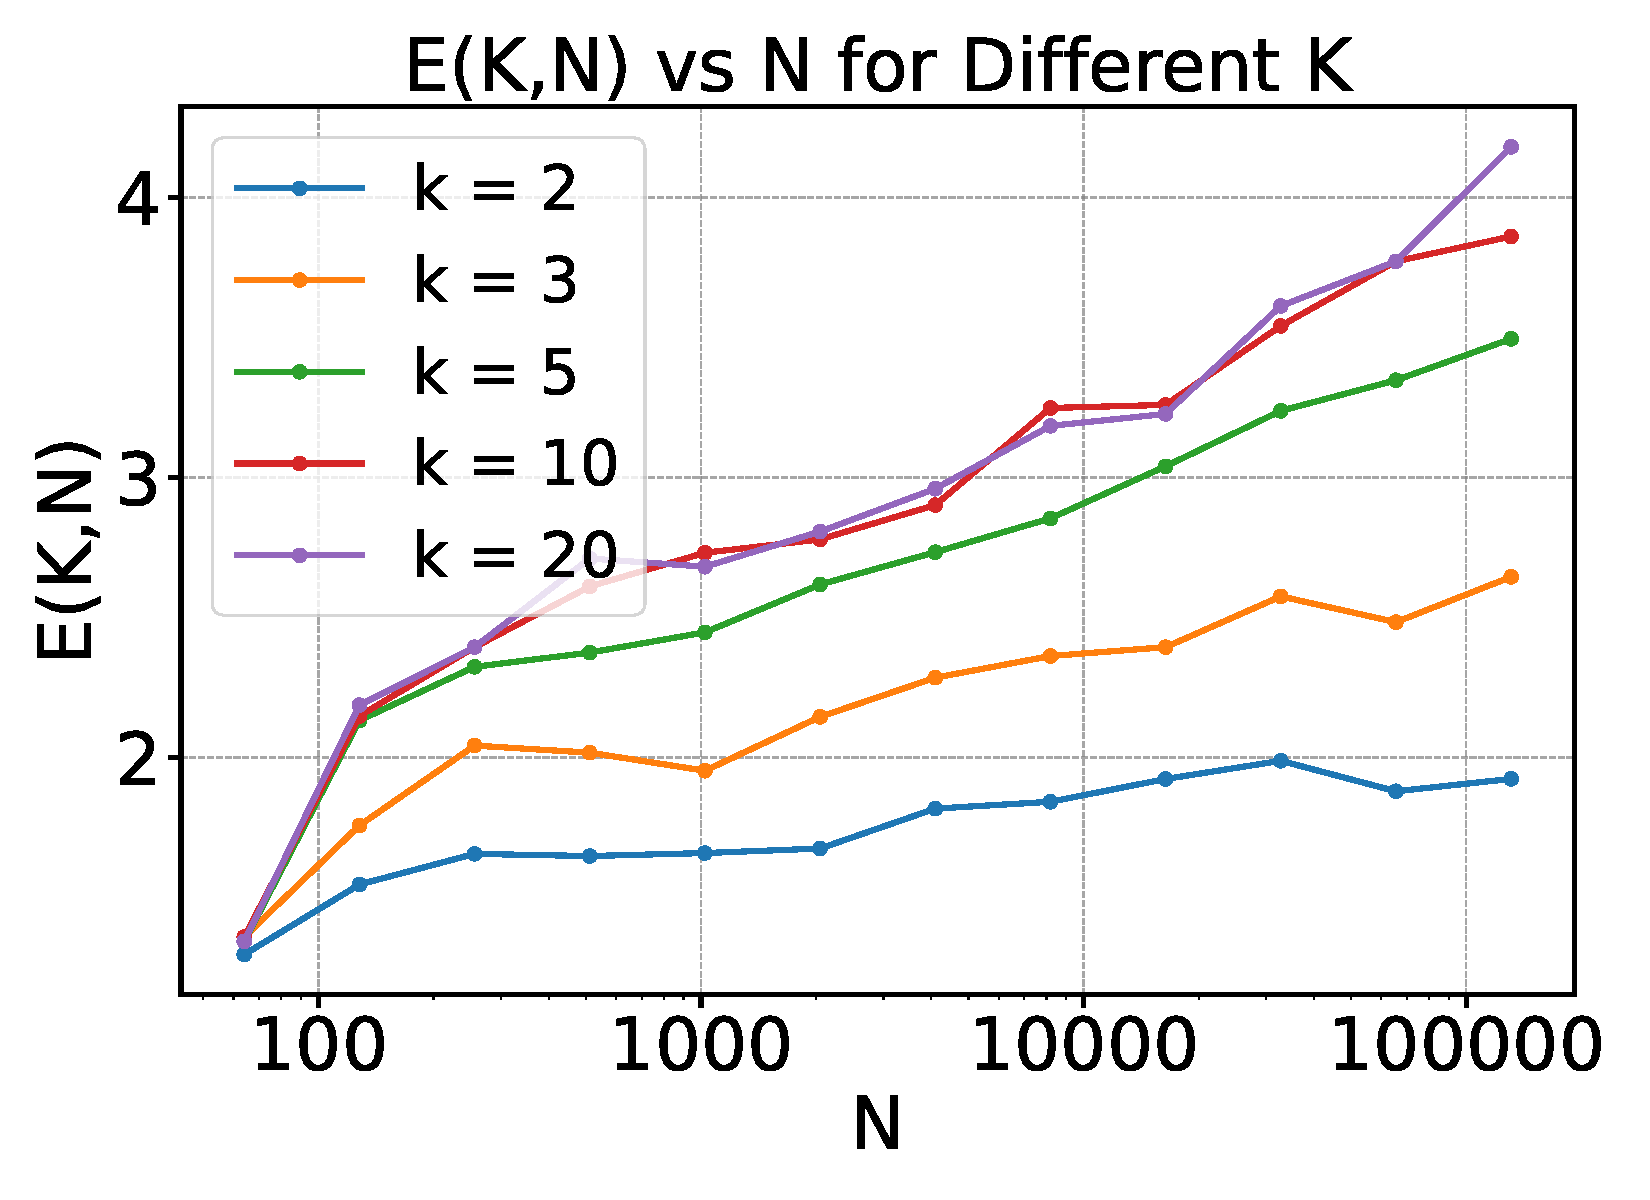
\includegraphics[width=\linewidth]{figs/E_k_avg_vs_N_log_wide_bold.pdf}
        \caption{Strongly convex case: $E(K,N)$ with $N$.}
        \label{fig:strongly-convex-EK-for-N}
    \end{subfigure}
    \begin{subfigure}[t]{0.634\linewidth}
        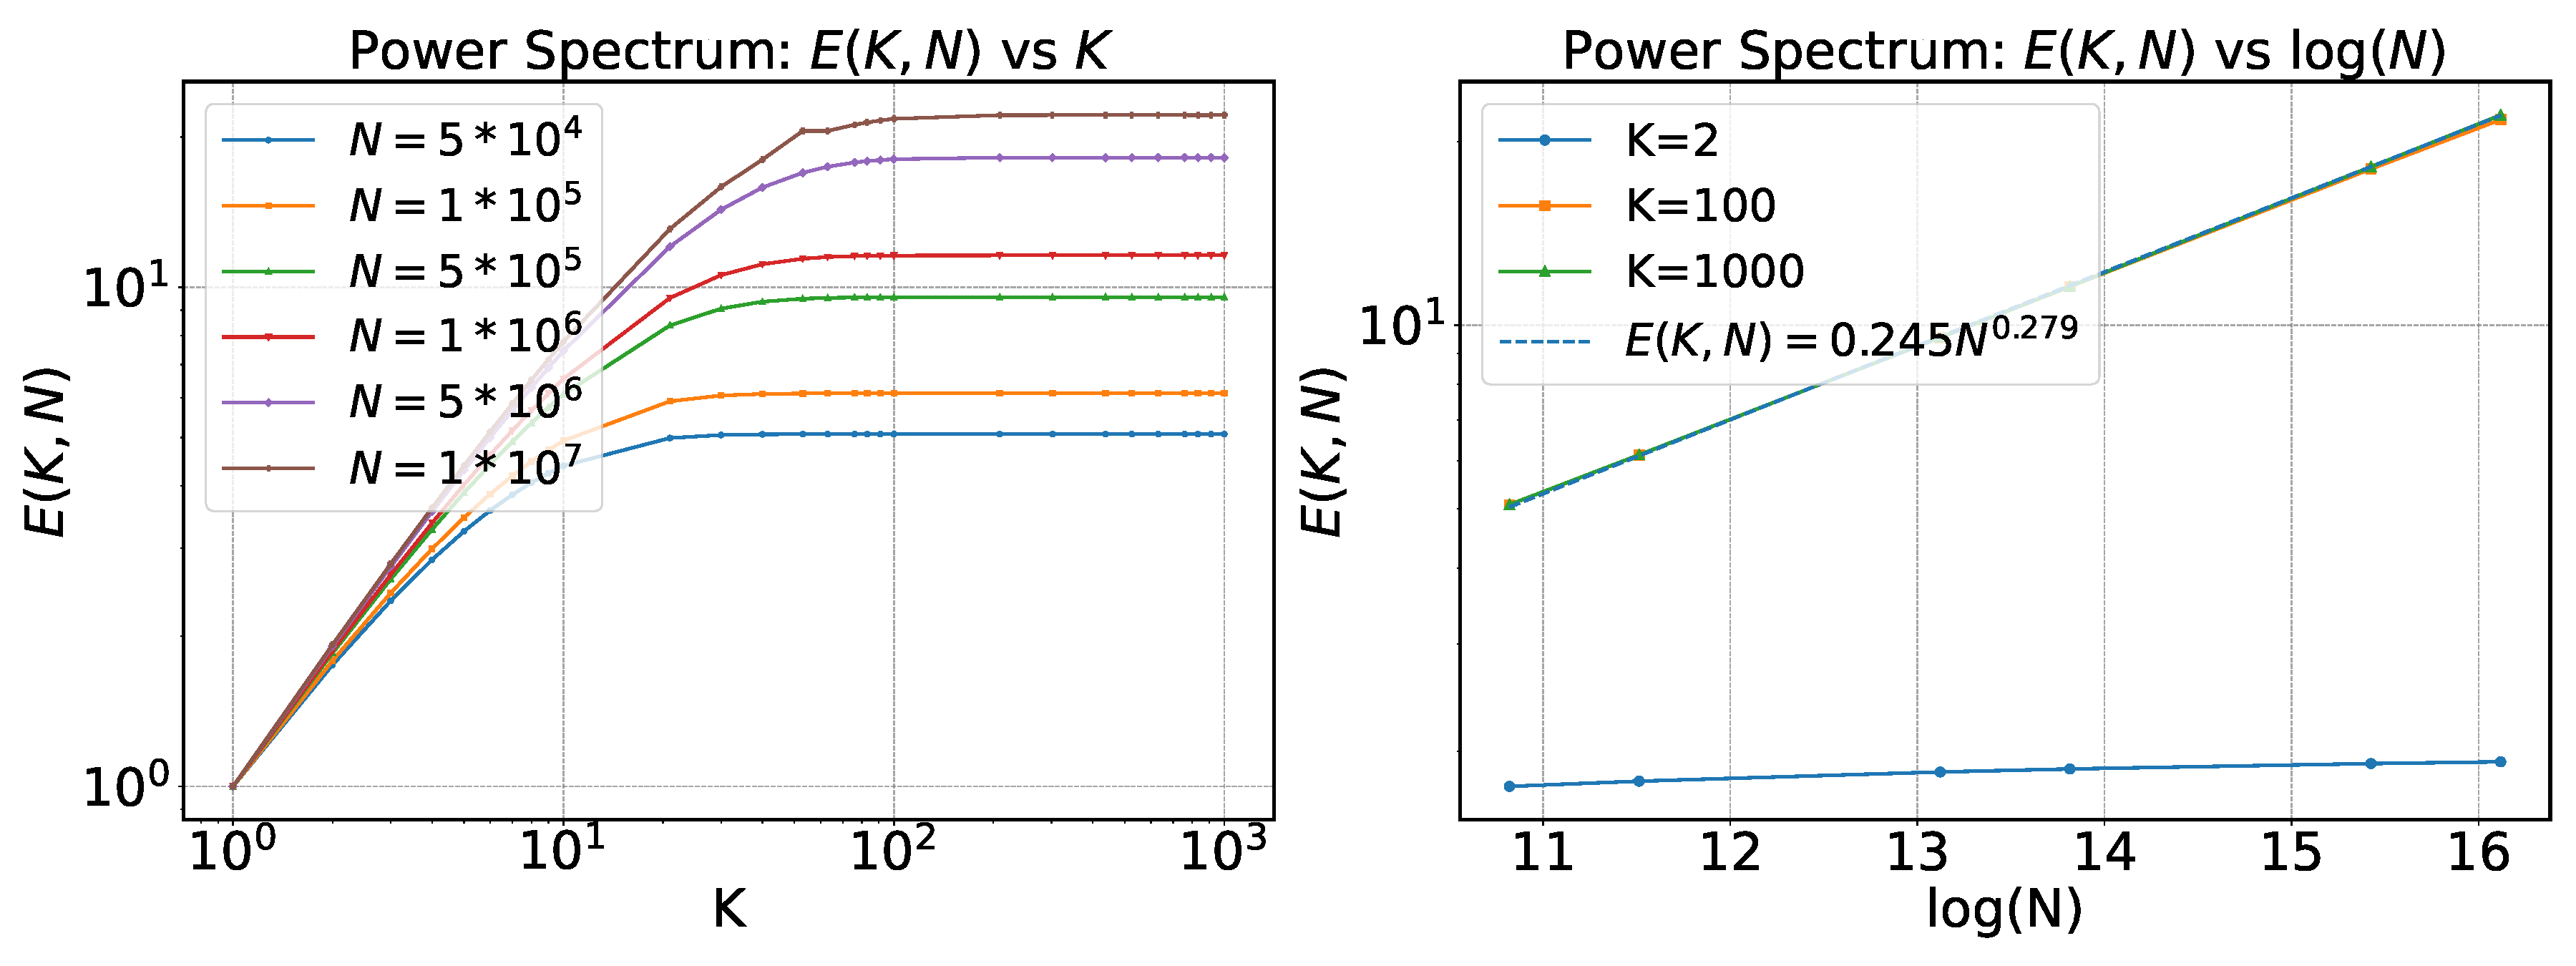
\includegraphics[width=\linewidth]{figs/E_K_comparison_power.pdf}
        \caption{\small The solvable case with Zipf-distributed data and power spectrum: $E(K,N)$ versus $K$ and $N$.}
        \label{fig:one-hot}
    \end{subfigure}
    \caption{\small Simulation experiments for strongly-convex linear regression and the solvable case with Zipf-distributed data and power spectrum. Results show that $E(K,N)$ is approximately proportional to some function of $N$ when $N$ is relatively small, and $E(K,N)\approx K$ when $N$ is relatively large. For the solvable case with Zipf-distributed data and power spectrum, we also fit the effective reuse rate using the formula $E(K,N)=c_1N^{c_2}$ suggested by \Cref{thm:one-hot-E_K-v2}, and the fitted exponent $c_2=0.279\approx\frac{b}{a-b}=\frac{2}{7}$ matches our theory.}
    % \haodong{rewrite the caption, reorganize the subfigures; replot the firgure (a), plot from $N=64$}
    % \tingkai{strongly-convex + power, put log into the appendix; delete the grid in strongly convex case}
% \vspace{-0.25in}
    \label{fig:convex-and-power}
\end{figure} 

%\subsection{Numerical Simulation in Synthetic Datasets}
%Now we validate our theory with experiments on synthetic data under two settings: one corresponding to the strongly-convex scenario of \Cref{sec:strongly_convex}, and another using the solvable model of \Cref{sec:one_hot}. 
\vspace{-0.3cm}
\subsection{Simulations in \Cref{sec:strongly_convex}}
% \vspace{-0.3cm}
% \tingkai{add section 5: power. add log into appendix.}

First, we conduct our experiments on synthetic datasets with a strongly convex linear regression to verify the characterization of effective reuse rate $E(K,N)$ in \Cref{thm:convex-E_K}.
% \kaifengclaw{Typo: 'on synthetic dataset' -> 'on a synthetic dataset' or 'on synthetic datasets'.} 

\paragraph{Experiments Setup.}  We generate data pairs $(\vx_i,y_i)$ where $\vx_i \overset{i.i.d}{\sim}\gN(0,\mI_d)$ with dimension $d = 100$. For the label $y_i$, we generate it as $y_i = \inp{\vw^*}{\vx_i} + \xi_i$, where $\vw^*$ is the ground truth generated by standard Gaussian with unit variance.
% \kaifengclaw{Typo: 'generate' -> 'generated'; 'Gaussin' -> 'Gaussian'.} 
Also, $\xi_i\overset{i.i.d}{\sim}\gN(0,\sigma^2\mI_d)$. Here in our simulation, we set $\sigma$ to $0.1$. To make our simulation aligned with the theoretical setup, we set the learning rate $\eta \propto \frac{\log KN}{KN}$, and we grid search the ratio $c:=\frac{\eta}{\log KN/KN}$ for the $c^*$ which minimizes the final loss given training steps $T=KN$. 

\paragraph{Results.} As shown in \Cref{fig:strongly-convex-EK-for-N}, we plot $E(K,N)$ as a function of $\log N$ for various fixed values of $K$. Each curve corresponds to a fixed number of epochs (e.g., $K=3,5,\dots,20$) and illustrates how the effective reuse rate $E(K,N)$ grows with dataset size. For small data size ($\log N \ll K$), the effective reuse factor increases roughly linearly with $\log N$, indicating that adding more data substantially boosts the one-pass equivalent performance. However, as $N$ becomes large ($\log N \gg K$), each curve flattens out and approaches an asymptote at $E(K,N)\approx K$. In other words, once the dataset is sufficiently large relative to the number of epochs, additional passes through the same data yield no further benefit beyond a factor of $K$. This behavior is exactly as predicted by \Cref{thm:convex-E_K}: when $K$ is much smaller than $\log N$, we have $E(K,N)\approx K$ (nearly full $K$-fold data reuse), whereas when $K$ is large relative to $\log N$, the effective reuse saturates and grows only on the order of $\log N$.

% \vspace*{-0.8cm}
\vspace{-0.4cm}
\subsection{Simulations in \Cref{sec:power-spectrum}} \label{sec:power-spectrum-experiment}
\vspace{-0.3cm}
We now verify the predictions of \Cref{thm:one-hot-E_K-v2} using synthetic data generated under the spectral assumptions of \Cref{sec:one_hot} 
% Because \Cref{thm:one-hot-loss-estimate} provides a closed-form expression for the multi-epoch loss in these settings, we can perform a more controlled simulation of $E(K,N)$. 
% In particular, we consider two cases: (i) 
with a power-law decay Hessian spectrum (\Cref{asp:prior-probability-and-norm}).
% , and (ii) a log-power decay spectrum (\Cref{asp:log-power-decay-prior}), corresponding to the conditions of \Cref{thm:one-hot-E_K-v2} and \Cref{thm:one-hot-E_K-log-spectrum}, respectively.
% \paragraph{Experiments Setup.} 
In all sub-figures of \Cref{fig:one-hot}, we set the data dimension $d$ to $10^5$ and tune all the learning rates to their optimal values. Here we set $a=4.5$ and $b=1$.
% \kaifengclaw{Possible typo: this sentence seems incomplete (likely intended '$a=4.5$ and $b=1$').} 

% . Additionally, we separately tune the spectrum parameters $a$ and $b$ in each sub-figure of \Cref{fig:one-hot}. Specifically, in the top-left and top-right panels, we set $a=4.5$ and $b=1$, whereas in the bottom-left and bottom-right panels, we set $a=1.5$ and $b=2$. 
% In the simulations of the power spectrum case, we 
% \paragraph{Simulations in Power Spectrum Case.} 
% The top-left panel of \Cref{fig:one-hot} plots $E(K,N)$ versus $\log K$ for various fixed $N$, while the right panels show $E(K,N)$ versus $\log N$ for various fixed $K$. In the power-law spectrum scenario, we observe an initial regime where $E(K,N)$ increases almost linearly with $K$ (indicating that more epochs initially provide almost proportional gains in effective data usage), followed by a clear saturation regime where $E(K,N)$ approaches a constant plateau even as $K$ continues to grow. This plateau value is much lower than $K$ when $K$ is large, and it depends on $N$ in a manner consistent with our theory. Specifically, $E(K,N)$ eventually saturates at an asymptotic value, and larger datasets yield higher saturation levels, reflecting a dataset-dependent multiple-epoch benefit, as predicted by \Cref{thm:one-hot-E_K-v2}.  

% % \begin{figure}[htbp]
% % \begin{figure}[t!]
% %     \centering
% %     \includegraphics[width=0.6\linewidth]{figures/one-hot-simulation/E_K_comparison_2x2_paper.pdf}
% %     \caption{Simulation results in the solvable case with power law. \textbf{Top-Left:}}
% %     \label{fig:one-hot}
% % \end{figure}

% \paragraph{Simulations in Log-Power Spectrum Case.} 
% In the log-power spectrum setting (bottom panels of \Cref{fig:one-hot}), $E(K,N)$ exhibits a similar two-regime behavior: the initial growth with $K$ transitions to a plateau whose height increases only logarithmically with $N$ (on the order of $\log^b N$), as described by \Cref{thm:one-hot-E_K-log-spectrum}. The curves depicting $E(K,N)$ versus $\log N$ further illustrate that, for fixed small values of $K$, increasing $N$ eventually yields diminishing returns as $E(K,N)$ approaches the $K$ limit (analogous to the strongly-convex case). For larger values of $K$, however, the effective multiplier reaches a ceiling determined by the dataset-dependent saturation value. These experiments demonstrate the anticipated saturation effects, multiple scaling regimes, and asymptotic plateaus, providing empirical confirmation of the scaling behaviors predicted by \Cref{thm:one-hot-E_K-v2} and \Cref{thm:one-hot-E_K-log-spectrum}.

\paragraph{Results.} \Cref{fig:one-hot} plots $E(K, N)$ versus $K$ and $\log N$ for the solvable model with Zipf-distributed  data. The curves depicting $E(K,N)$ versus $K$ show that $E(K,N)\approx K$ when $K$ is relatively small and saturate to some value depending on $N$ when $K$ is large. In the right panel, which describes the relationship between $E(K,N)$ and $\log N$, we observe that when $K$ is small (namely $K=2$), $E(K,N)$ increases and approaches $K$ as $\log N$ increases, and the plots overlap when $K$ is large. Those phenomena provide empirical confirmation of the scaling behaviors predicted by \Cref{thm:one-hot-E_K-v2}. We also fit $E(K,N)$ in the large-$K$ regime with a power-form function as stated in \Cref{thm:one-hot-E_K-v2}. The fitted exponent is $0.279 \approx \tfrac{b}{a-b} = \tfrac{2}{7}$, aligning with our theory.
% \begin{figure}[t]
% \vspace{-0.5in}
%     \centering
%     \includegraphics[width=0.5\linewidth]{figures/strongly-convex/E_k_avg_vs_N_log_wide_bold.pdf}
%     \caption{Strongly convex case: $E(K,N)$ with $N$}
%     \label{fig:strongly-convex-EK-for-N}
% \vspace{-0.25in}
% \end{figure}

% \begin{figure}[t]
% % \vspace{-0.6in}
%     \centering
%     \begin{subfigure}[b]{0.48\linewidth}
%         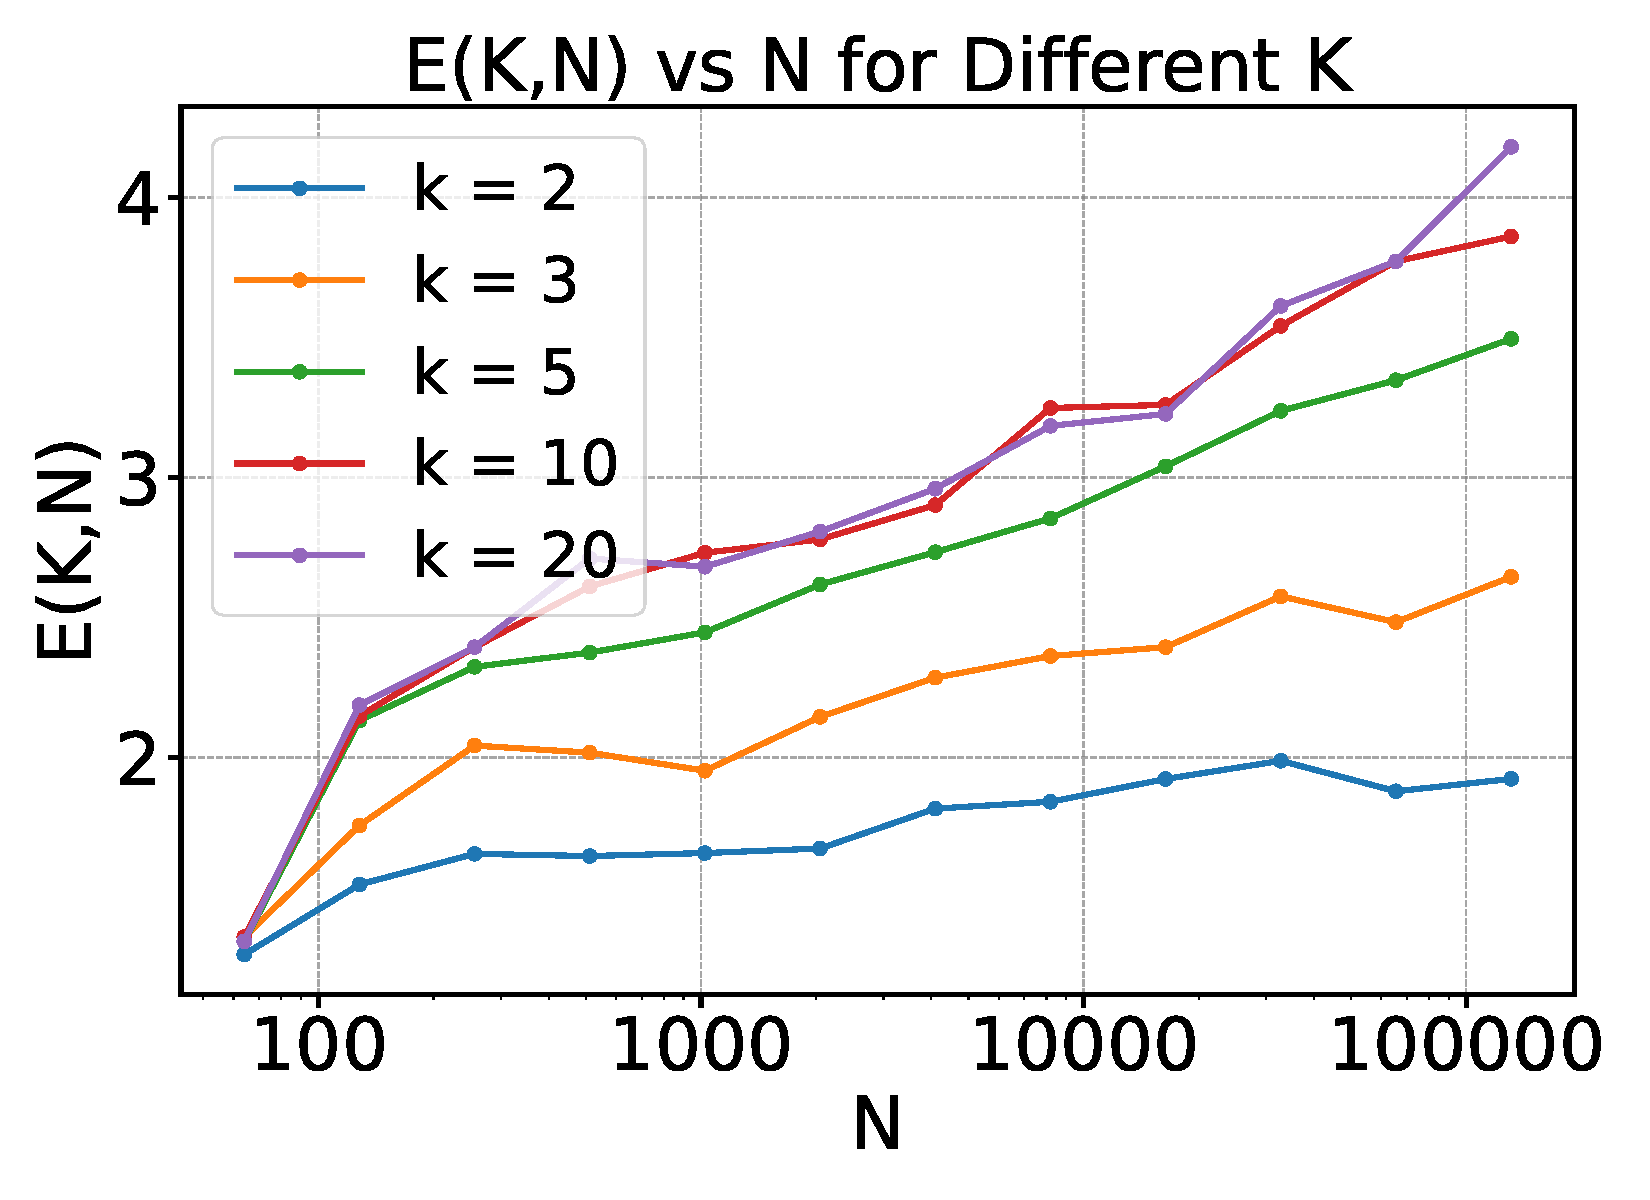
\includegraphics[width=\linewidth]{figs/E_k_avg_vs_N_log_wide_bold.pdf}
%         \caption{Strongly convex case: $E(K,N)$ with $N$}
%         \label{fig:strongly-convex-EK-for-N}
%     \end{subfigure}
%     \begin{subfigure}[b]{0.48\linewidth}
%         \includegraphics[width=\linewidth]{figs/E_K_comparison_2x2_paper.pdf}
%         \caption{The solvable cases with power law in simulation.}
%         \label{fig:one-hot}
%     \end{subfigure}
%     \caption{Simulation Experiments.}
% % \vspace{-0.25in}
% \end{figure}

% \begin{figure}[t]
%     \centering
%     \subfigure[Strongly convex case: $E(K,N)$ with $N$%
%       \label{fig:strongly-convex-EK-for-N}]{
%         \includegraphics[width=0.48\linewidth]{figs/E_k_avg_vs_N_log_wide_bold_0830.pdf}
%     }\hfill
%     \subfigure[The solvable cases with power law in simulation.%
%       \label{fig:one-hot}]{
%         \includegraphics[width=0.48\linewidth]{figs/E_K_comparison_2x2_paper.pdf}
%     }
%     \caption{Simulation Experiments.}
% \end{figure}

% \begin{figure}[t]
% % \vspace{-0.6in}
%     \centering
%     \begin{subfigure}[t]{0.326\linewidth}
%         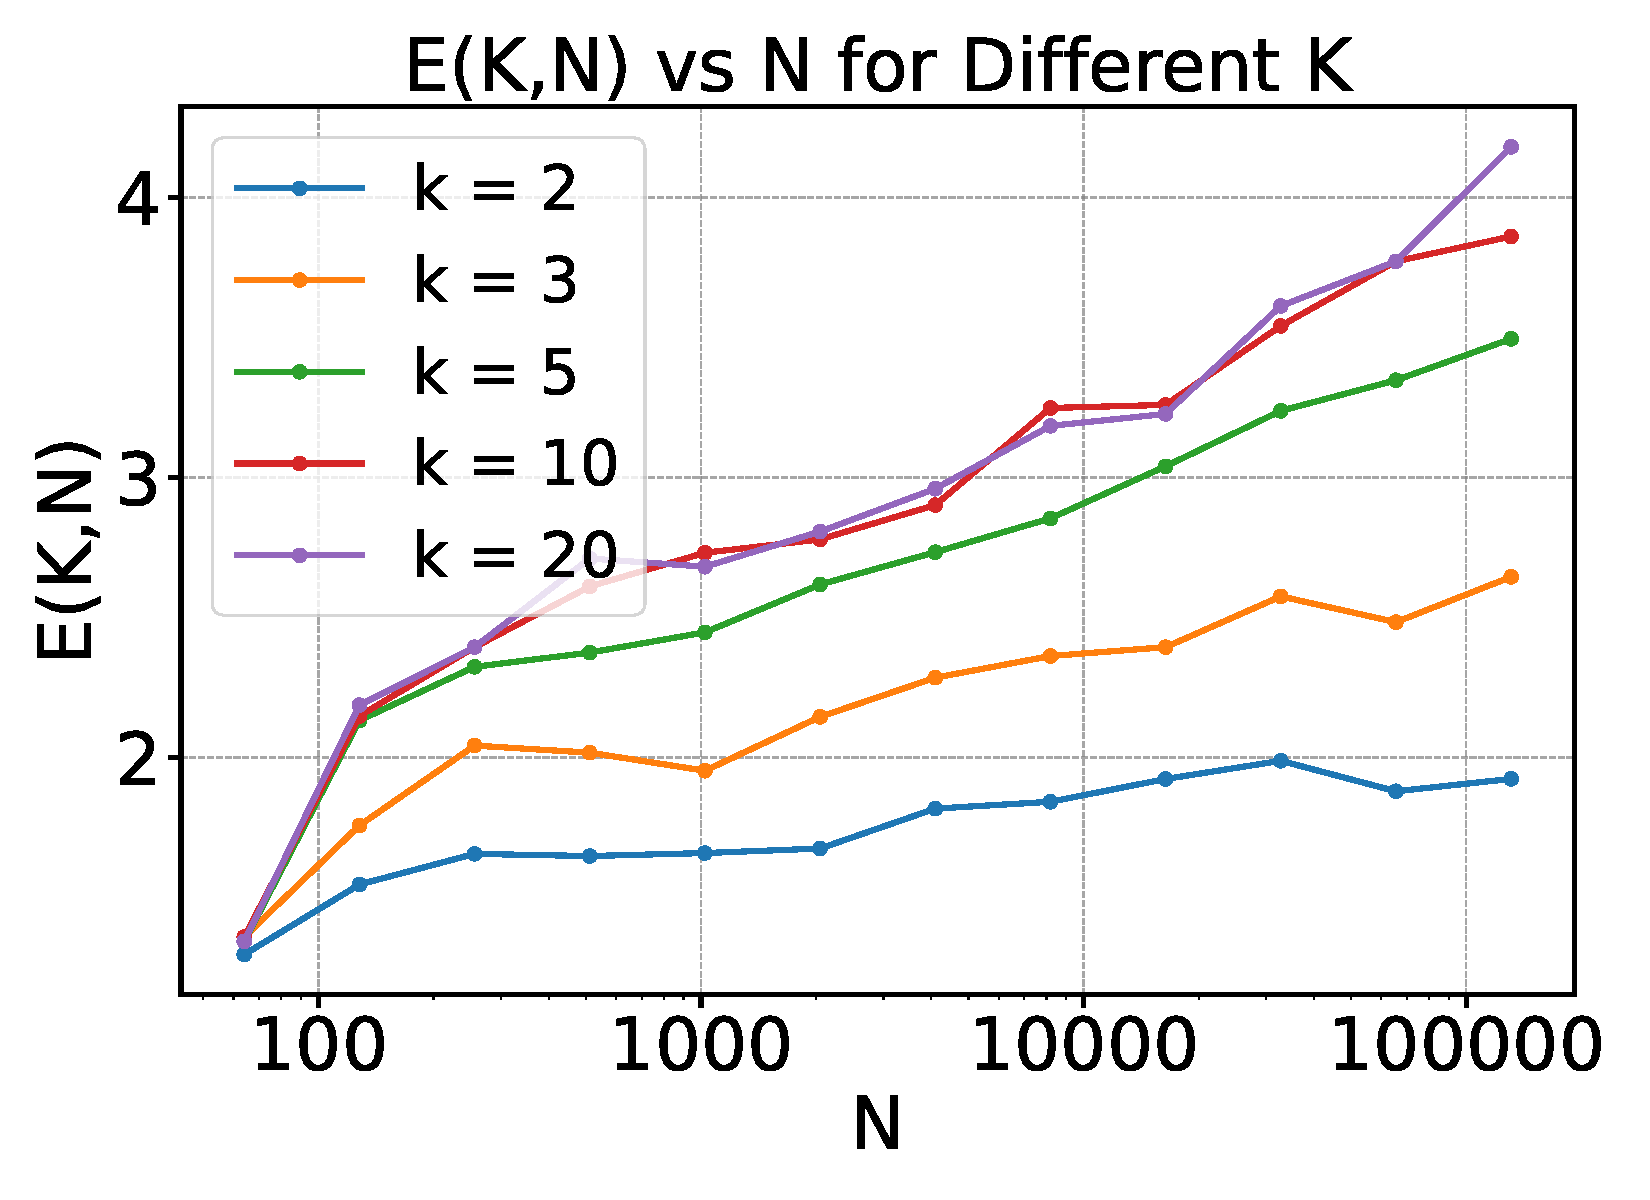
\includegraphics[width=\linewidth]{figs/E_k_avg_vs_N_log_wide_bold.pdf}
%         \caption{Strongly convex case: $E(K,N)$ with $N$}
%         \label{fig:strongly-convex-EK-for-N}
%     \end{subfigure}
%     \begin{subfigure}[t]{0.634\linewidth}
%         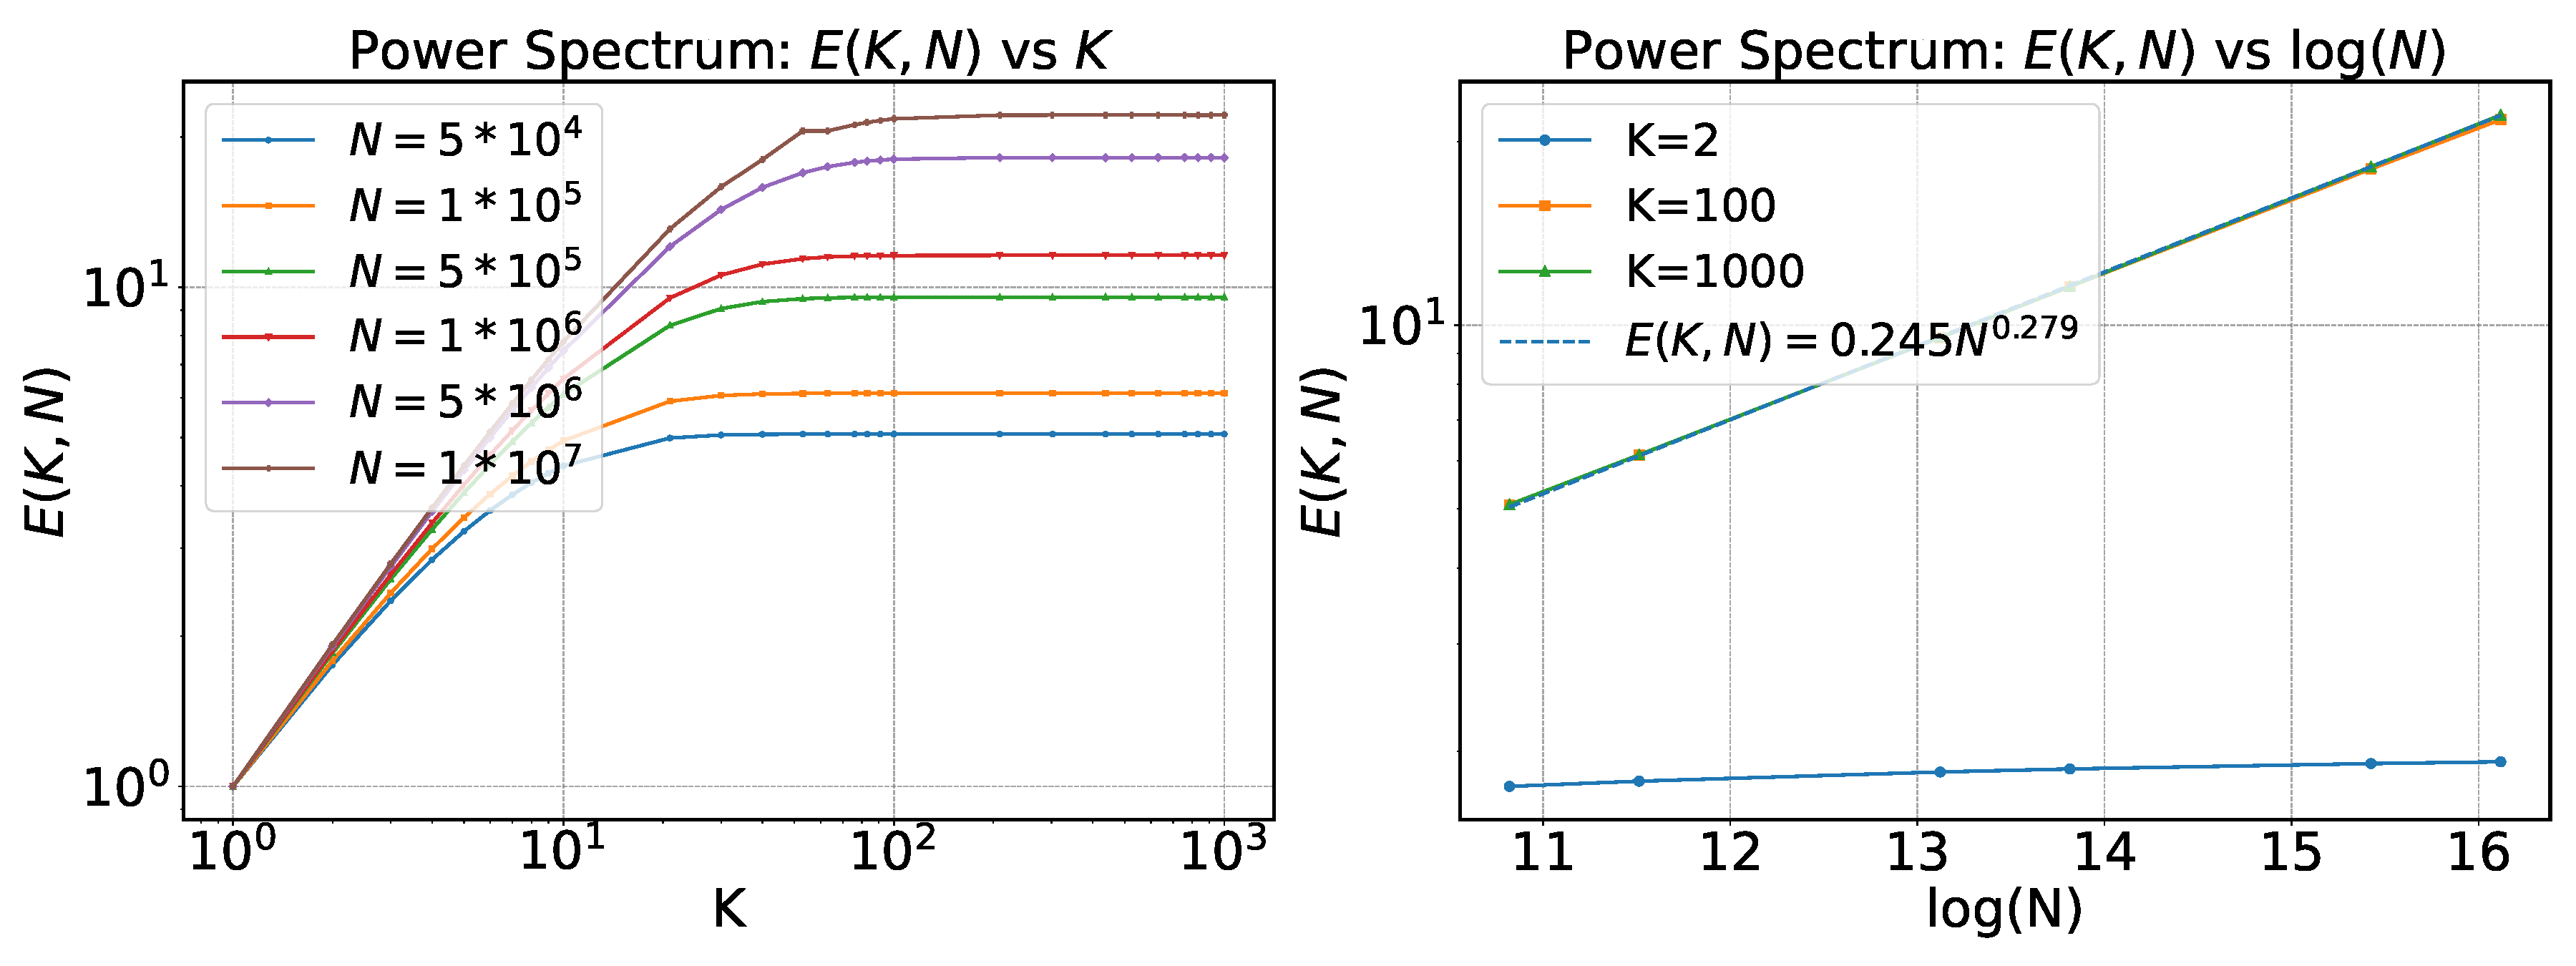
\includegraphics[width=\linewidth]{figs/E_K_comparison_power.pdf}
%         \caption{The solvable cases with power law in simulation.}
%         \label{fig:one-hot}
%     \end{subfigure}
%     \caption{Simulation Experiments.}
%     % \haodong{rewrite the caption, reorganize the subfigures; replot the firgure (a), plot from $N=64$}
%     % \tingkai{strongly-convex + power, put log into the appendix; delete the grid in strongly convex case}
% % \vspace{-0.25in}
% \end{figure}
% \vspace{-0.2in}
\subsection{Empirical Validation on Large Language Models}\label{sec:experiment-llm}

% To examine whether our theoretical predictions on effective reuse rate hold on different large language model training regimes and model sizes, we conduct experiments on two representative large language models: a 0.3B-parameter model trained from scratch and a 1.7B-parameter model fine-tuned on downstream data. The 0.3B pretraining experiment, which provides a direct verification of our theory, is described in the main text. The 1.7B fine-tuning experiment is presented in \Cref{app:metamath_experiment} due to space constraints.
% \vspace{-0.2mm}

% \begin{figure}[htbp]
   % \begin{subfigure}[b]{0.48\linewidth}
    %     \includegraphics[width=\linewidth]{figures/LLM/loss_over_step.pdf}
    %     \caption{Training loss as a function of training steps for different fresh data sizes.}
    %     \label{fig:loss-step}
    % \end{subfigure}
% \begin{figure}[t!]
%     % \vspace{-0.7in}
%     \centering
%     \begin{subfigure}[b]{0.48\linewidth}
%          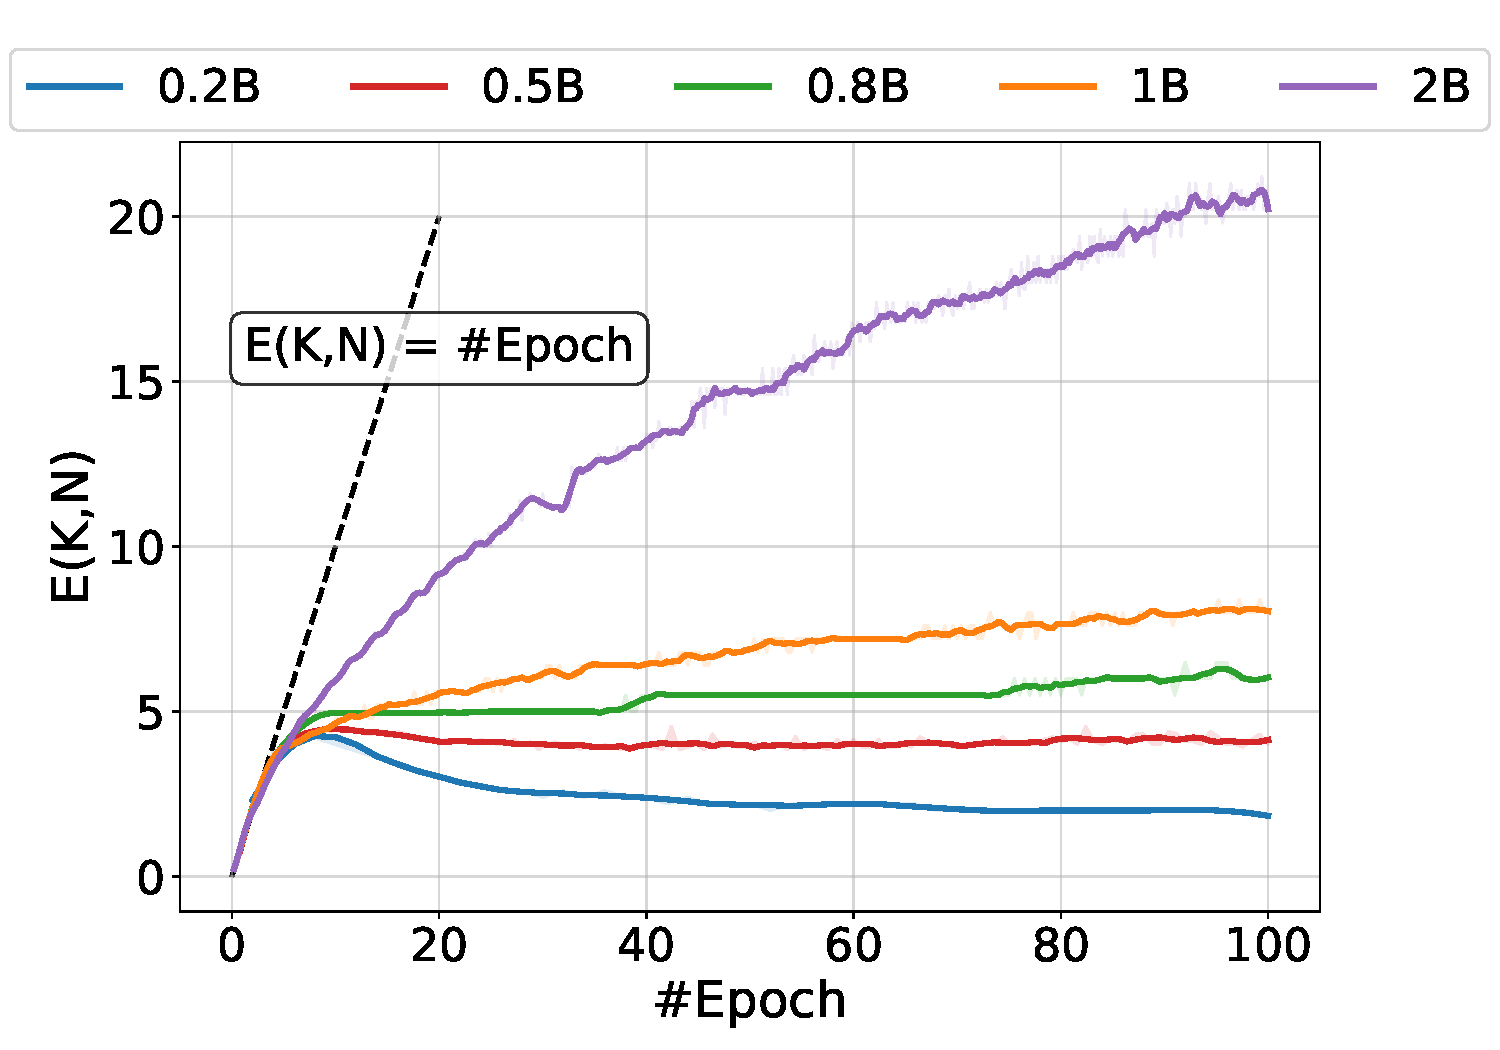
\includegraphics[width=\linewidth]{figs/E_k_smoothed_shaded.pdf}
%          \caption{The effective reuse rate $E(K,N)$ as a function of the epoch number $K$.}
%         % \caption{The effective reuse rate $E(K,N)$ as a function of the number of training epochs $K$ for varying fresh data sizes $N$. The shaded regions represent the variability from the smoothed trend in different epochs.}
%         \label{fig:ek-k}
%     \end{subfigure}   
%     \hfill
%     \begin{subfigure}[b]{0.48\linewidth}
%         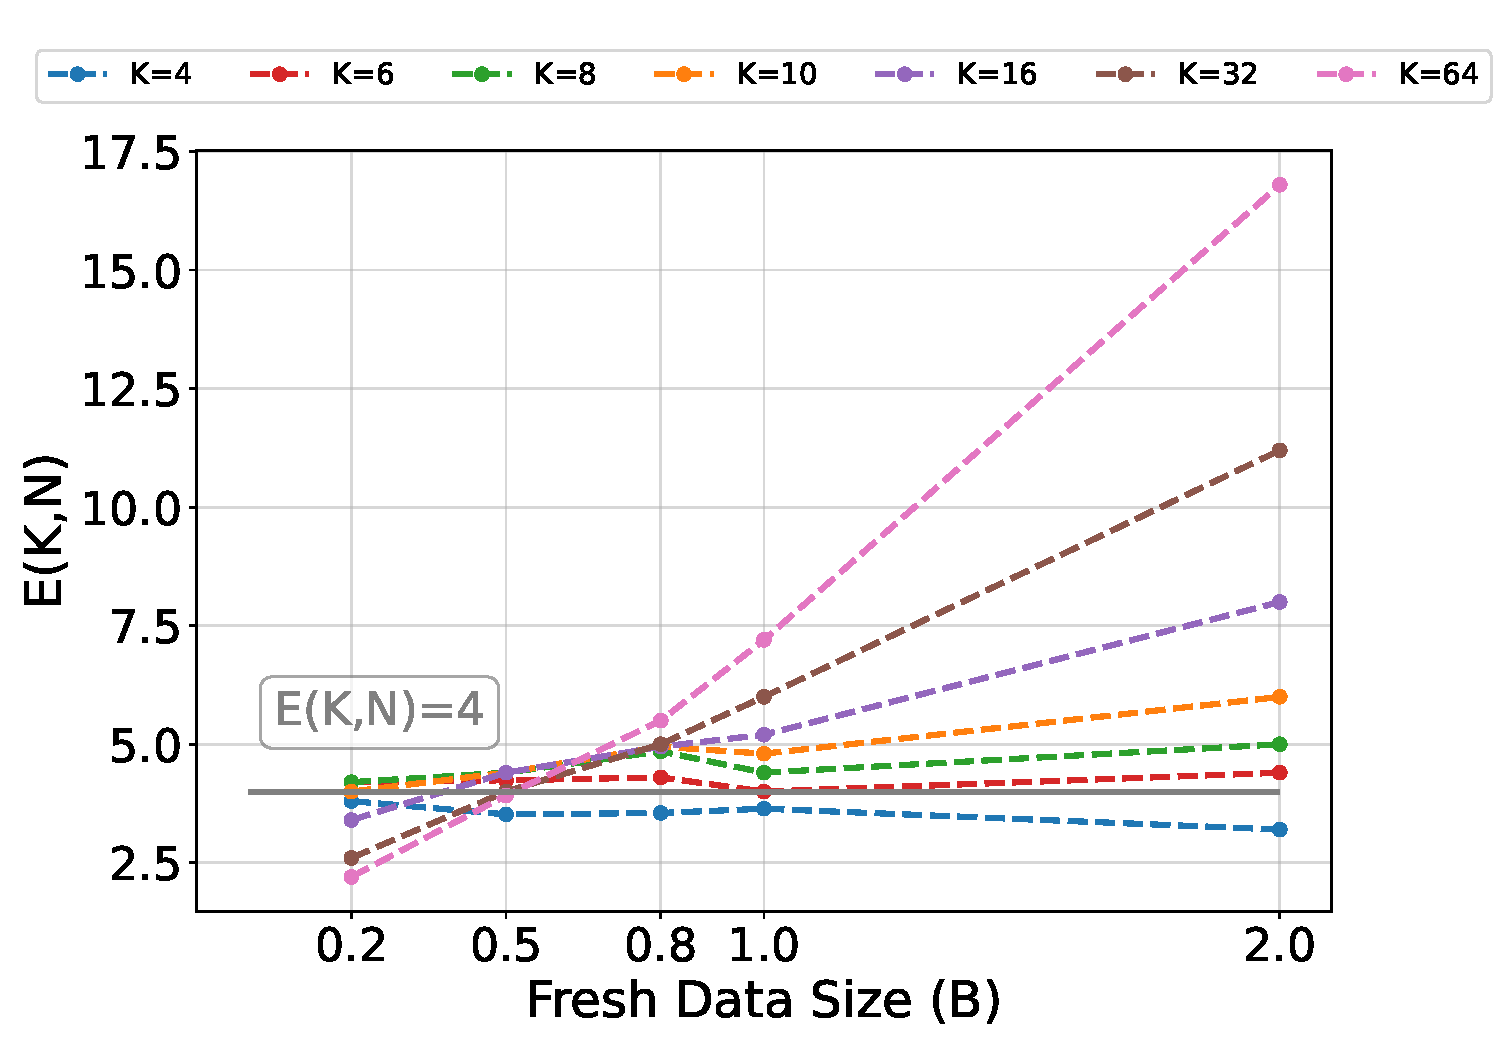
\includegraphics[width=\linewidth]{figs/E_k_over_fresh_data_size.pdf}
%         \caption{The effective reuse rate $E(K,N)$ as a function of the fresh data size $N$.}
%         \label{fig:ek-data}
%     \end{subfigure}
%     \caption{The effective reuse rate $E(K,N)$ over $K$ and $N$ in language model experiments.}
%     % \caption{}
%     % \caption{\textbf{Left:} Training loss progression over training steps. \textbf{Right:} The saturated effective reuse rate $E(K,N)$ in relation to the size of the fresh dataset $N$.}
%     % \vspace{-0.2in}
% \end{figure}

% \begin{figure}[t]
%     % \vspace{-0.4in}
%     \centering
%     \includegraphics[width=0.5\linewidth]{figs/E(K, N) vs N_ws3_ratio0.75_alpha0.9_exp.pdf}
%     \caption{The saturation points $K(\lambda,N)$ as a function of the dataset size N.}
%     \label{fig:ek-n-saturation point}
%     \vspace{-0.2in}
% \end{figure}


\begin{comment}
\begin{figure}[t!]
    \centering
    \subfigure[The effective reuse rate $E(K,N)$ as a function of the epoch number $K$.%
      \label{fig:ek-k}]{
        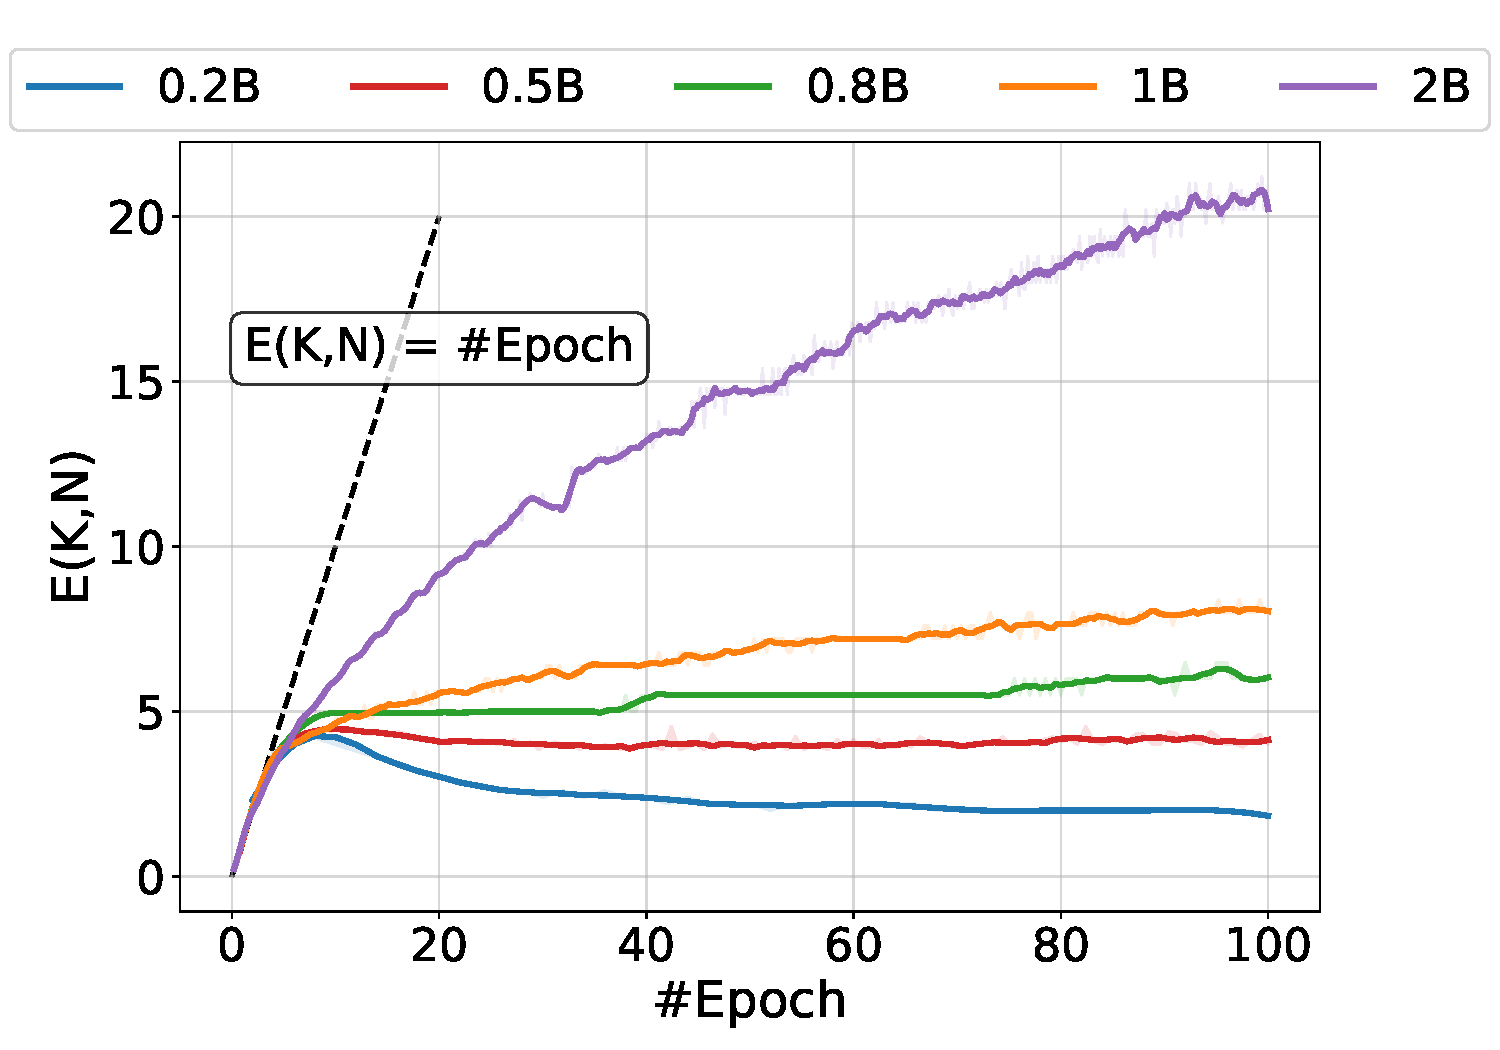
\includegraphics[width=0.48\linewidth]{figs/E_k_smoothed_shaded.pdf}
    }\hfill
    \subfigure[The effective reuse rate $E(K,N)$ as a function of the fresh data size $N$.%
      \label{fig:ek-data}]{
        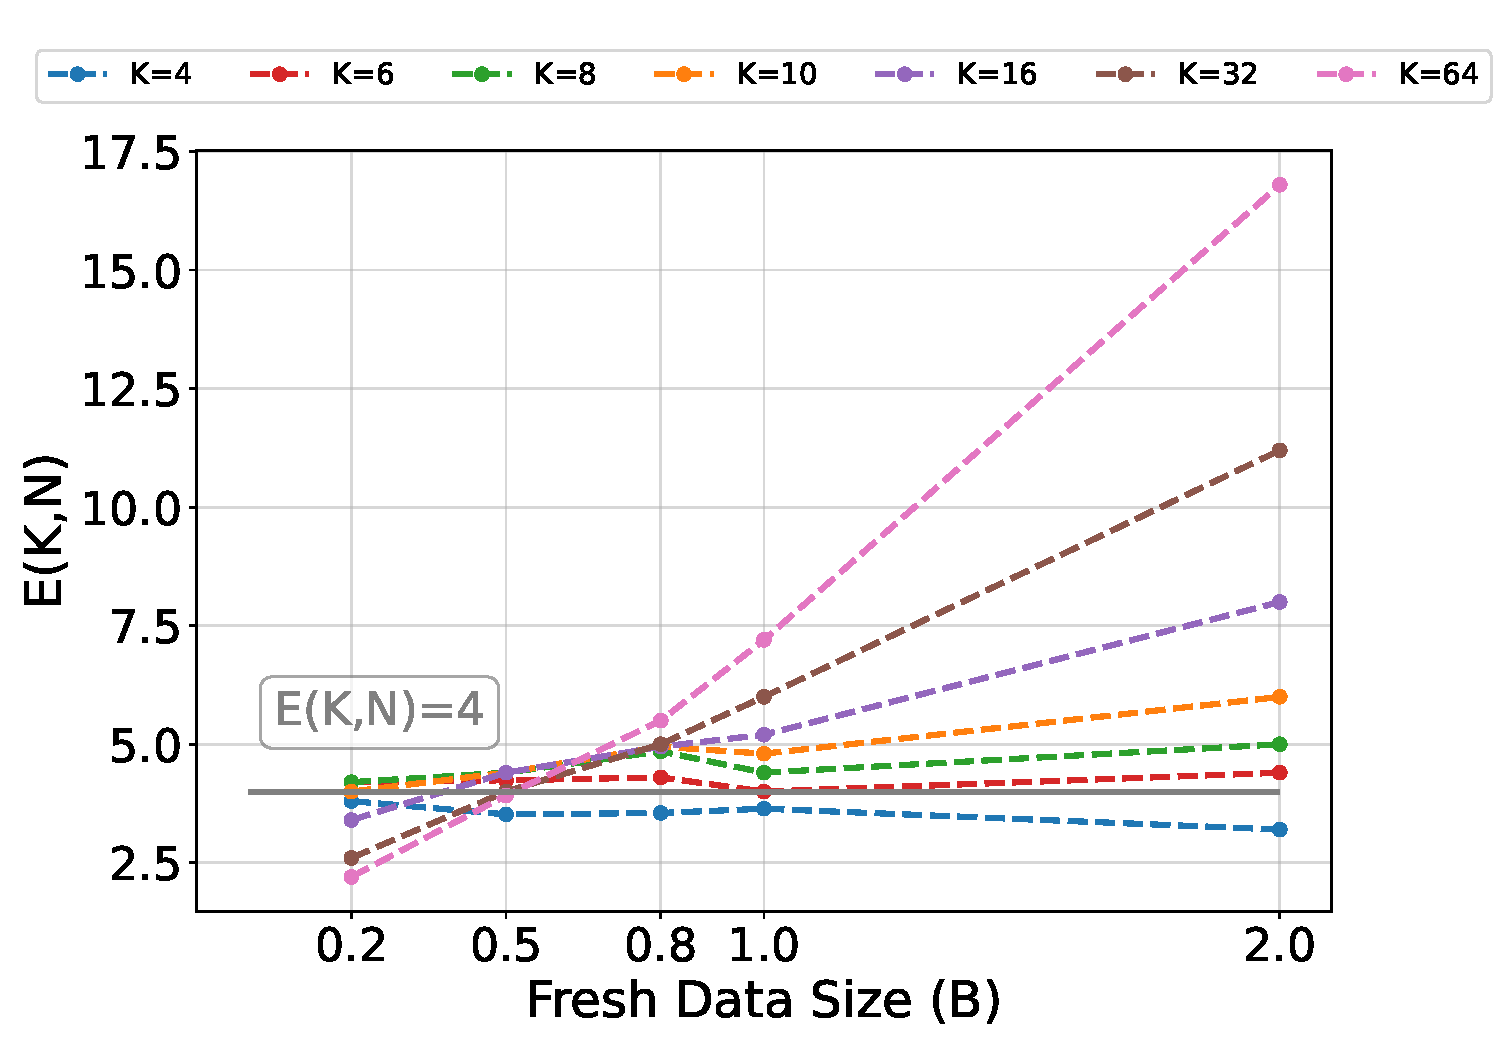
\includegraphics[width=0.48\linewidth]{figs/E_k_over_fresh_data_size.pdf}
    }
    \caption{The effective reuse rate $E(K,N)$ over $K$ and $N$ in language model experiments.}
\end{figure}
\end{comment}


% \paragraph{Experiments Setup.} To empirically validate that larger datasets enable more effective repetition, we pretrained a large language model with fresh data sizes from 0.2B to 2B tokens (100 epochs each), and a 200B-token control. The effective reuse rate, $E(K,N) = N_f(K,N)/N$, was approximated by determining the fresh data size $N_f(K,N)$ for equivalent single-pass validation loss. We used a 0.3B parameter model (adapted from Qwen2.5-0.5B~\citep{qwen2025qwen25technicalreport}), a 200B-token DCLM subset, and a constant learning rate (to align with theory and avoid learning rate effects~\citep{hoffmann2022training,luo2025multi}). See \Cref{app:setup} for details.

% \paragraph{When $K\le 4$, $E(K,N) \approx K$.} Our theory predicts $E(K,N) \approx K$ for small $K$ (e.g., $K\le 4$). \Cref{fig:loss-step} shows that insufficient data (0.2B tokens) leads to overfitting, which is reduced by larger datasets. Consequently, the difference between multi-epoch and single-pass performance decreases. As shown in \Cref{fig:ek-k,fig:ek-data}, $E(K,N)$ increases with $K$ for small $K$ ($\approx K$ for $K\le 5$) and saturates near $K$ at $K=4$, aligning with data-constrained scaling laws~\citep{muennighoff2023scaling}.

% \paragraph{Larger Datasets Allow More Repetition.} $E(K,N)$ increases with epochs and saturates (towards $K$) for sufficiently large datasets, challenging the assumption of a uniform effective number of epochs across dataset sizes in~\citet{muennighoff2023scaling}. \Cref{fig:ek-data} shows $E(K,N)$ increases monotonically with dataset size (before saturating to $K$, as seen for $K\ge 16$). With 2B tokens, $E(K,N)$ continues to grow after 100 epochs (\Cref{fig:ek-k}), implying that repeating 2B tokens 100 times is equivalent to using over 40B fresh tokens, and suggesting further pretraining scaling with larger datasets.

\paragraph{Experiments Setup.} We conduct experiments on a large language model to empirically validate the hypothesis that larger datasets allow for more effective repetition. We perform pretraining runs with fresh data sizes of 0.2B, 0.5B, 0.8B, 1.0B, and 2B tokens, each trained for 100 epochs. As a control, we also include a run with 200B fresh tokens. For each fresh dataset size $N$ and training epoch $K$, we approximate the effective reuse rate $E(K,N)$ by determining the effective fresh data size $N_f(K,N)$ required to achieve the same validation loss after one pass through the data. The effective reuse rate is then computed as: $E(K,N)=\frac{N_f(K,N)}{N}$.
% \label{eq:llm}

Our experiments utilize a 0.3B parameter model adapted from the Qwen2.5-0.5B architecture~\citep{qwen2025qwen25technicalreport} and a subset of the DCLM dataset, totaling 200B tokens.
%The smaller-than-standard model size is chosen due to the substantial computational cost associated with multi-epoch pretraining.
A separate subset of the DCLM dataset is reserved for validation. Crucially, we use a constant learning rate schedule across all experiments to align with our theoretical analysis and mitigate the confounding effects of learning rate schedules, as reported in prior work~\citep{hoffmann2022training,luo2025multi}. ~\Cref{fig:ek-k} depicts the relationship between $E(K,N)$ and $K$. ~\Cref{fig:loss-step} depicts the training curves for different data sizes, and marks the points of different curves where $E(K,N)=\lambda K$, where $\lambda$ controls how strict the criterion is for determining when multi-epoch training begins to underperform one-pass training. Given such $\lambda$, we denote the corresponding number of training epochs as $K(\lambda, N)$, which we refer to as \textit{saturation points}. In our experiments, we take $\lambda = 0.75$. Further, in \Cref{fig:ek-n-saturation point}, we show the precise relationship between $K(\lambda, N)$ and $N$. More details regarding the experiment setup are available in Appendix~\ref{app:setup}.


% These points mark where multi-epoch training begins to underperform compared with single-epoch training. 
% We compute $E(K,N) = \lambda K$ for $11$ uniformly spaced values of $\lambda$ in the range $[0.8,0.9]$ and average the resulting $E(K,N)$ values as the separation point value. Here we use multiple values of $\lambda$ because the curve exhibits randomness, and averaging over several choices yields a more reliable trend. 




% Moreover, model size is also a key factor in real LLM training.
% Furthermore, in Figure~3 we visualize, for each fresh data size $N$, the saturation-point value of $E(K,N)$ at which multi-epoch training first starts to underperform the one-pass baseline. This shows how the recommended effective reuse rate varies with $N$, and we fit these saturation points as a function of $N$ to obtain an empirical rule for choosing the number of passes; see Appendix~C.2 for details of the fitting procedure. To assess the robustness of our conclusions with respect to the learning-rate schedule, we additionally repeat the analysis under a trapezoidal learning-rate schedule; the experimental setup and results are described in Appendix~C.3.


% \begin{figure}[t]
%     % \vspace{-0.4in}
%     \centering
%     \includegraphics[width=0.5\linewidth]{figs/E(K, N) vs N_ws3_ratio0.75_alpha0.9_exp.pdf}
%     \caption{The saturation points $K(\lambda,N)$ as a function of the dataset size N.}
%     \label{fig:ek-n-saturation point}
%     \vspace{-0.2in}
% \end{figure}

\paragraph{Previous Work: When $K\le 4$, $E(K,N) \approx K$.} Our theoretical analysis indicates that $E(K,N)$ should be close to $K$ when $K$ is small (e.g., $K\le 4$). 
% In \Cref{fig:loss-step}, we show the validation losses for different fresh data sizes as they vary with the training steps. When the fresh data is insufficient, such as 0.2B tokens, the training run experiences overfitting, where the validation loss starts to increase as training progresses. As the fresh data size increases, the validation loss decreases at the same training step. Furthermore, the performance difference between multi-epoch training and a single pass through the data becomes smaller with larger fresh datasets. Computing $E(K, N)$, we present the variation of $E(K, N)$ with both $K$ and $N$ in~\Cref{fig:ek-k,fig:ek-data}.
In Figure~\ref{fig:ek-k}, when the epoch number is small (approximately $\le 5$), we observe that $E(K,N)$ increases at a rate comparable to the epoch number, 
as indicated by the black dashed line. 
% Moreover, in the case of $K=4$, $E(K,N)$ saturates close to $K$ across different fresh data sizes, as depicted by the blue line and gray baseline in~\Cref{fig:ek-data}. 
Thus our predictions of $E(K,N)$ when $K$ is small aligns with the data-constrained scaling laws~\citep{muennighoff2023scaling}. 

\paragraph{Larger Datasets Allow More Repetition.}
$E(K,N)$ increases with the number of fresh data sizes and eventually saturates 
% (towards $K$) 
for sufficiently large fresh datasets. Our results challenge the data-constrained scaling laws proposed by~\citet{muennighoff2023scaling}, which assume a uniform effective number of epochs across different fresh data sizes. In Figure~\ref{fig:loss-step}, we show that at the critical points where one-pass training start to outperform multi-epoch training significantly, $E(K,N)$ increases as $N$ increases. This suggests the continued potential for scaling pretraining through multi-epoch training with larger datasets.


% \haodong{replace tuning point with saturation point or Separation point, anyway, give it a clear definition}
\paragraph{Fitting Experiments.}In \Cref{fig:ek-n-saturation point}, to provide real-world evidence that larger datasets can be repeated more, we plot the saturation point values for different $N$ to illustrate how they vary with $N$. Then we fit them as a function of $N$; see Appendix~\ref{app:fitting experiments} for details of the fitting procedure. 

% Further, we show the precise relationship between the saturation points and $N$ in \Cref{fig:ek-n-saturation point}. 
Surprisingly, though we do not claim that $E(K,N) = \Theta(\log N)$ holds for general LLM trainings when $K$ is large, as we calculated in the strongly convex linear regression case, here we do observe that $K(\lambda,N)$ gradually increases when $N$ increases, and it follows that $K(\lambda,N) \approx 0.80 \log N + 5.21$ with the correlation coefficient being $r = 0.97$. In this formula, the dataset $N$ is measured in billions of tokens (B).

\paragraph{Experiments with Learning Rate Decay.}For further investigation of the scaling behaviour of multi-epoch training, we conduct LLM experiments with a non-constant learning rate schedule, aligning with the common practice in reality. Specifically, we additionally repeat the above analysis with a WSD learning rate schedule with linear decay. The experimental setup and results are described in Appendix~\ref{app:experiment-llm-lrs}.

% \paragraph{Limitations of LLM experiments.} 


% characterizes this relationship precisely, namely $E(K,N) = \Theta\left(\log N\right)$, with the correlation coefficient of the fit being $r=0.99$.
% In contrast, as clearly presented in \Cref{fig:ek-data}, for the same epoch number, $E(K,N)$ values monotonically increase with the fresh data size before $E(K,N)$ saturates to $K$, as seen in cases with $K\ge 16$ in our experiment. Furthermore, except in the insufficient fresh data scenario (before saturation), the effective reuse rate monotonically increases as the epoch number increases. Remarkably, even after 100 repetitions with a large fresh dataset size (2B tokens in our experiment), the effective number of epochs has not yet converged, as shown in~\Cref{fig:ek-k}. Specifically, repeating 2B data for 100 epochs is equivalent to over 40B fresh data based on validation loss. 


% \kairong{Align notations with theory part.}
% \paragraph{Experiments Setup.} We conduct experiments on a large language model to empirically validate the hypothesis that larger datasets allow for more effective repetition. We perform pretraining runs with fresh data sizes of 0.2B, 0.5B, 0.8B, 1.0B, and 2B tokens, each trained for 100 epochs. As a control, we also include a run with 200B fresh tokens. For each fresh dataset size $N$ and training epoch $K$, we approximate the effective reuse rate $E(K,N)$ by determining the effective fresh data size $N_f(K,N)$ required to achieve the same validation loss after one pass through the data. The effective reuse rate is then computed as:
% \begin{equation}\label{eq:llm}
%     E(K,N)=\frac{N_f(K,N)}{N}.
% \end{equation}
% Our experiments utilize a 0.3B parameter model adapted from the Qwen2.5-0.5B architecture~\citep{qwen2025qwen25technicalreport} and a subset of the DCLM dataset, totaling 200B tokens. The smaller-than-standard model size is chosen due to the substantial computational cost associated with multi-epoch pretraining. A separate subset of the DCLM dataset is reserved for validation. Crucially, we use a constant learning rate schedule across all experiments to align with our theoretical analysis and mitigate the confounding effects of learning rate schedules, as reported in prior work~\citep{hoffmann2022training,luo2025multi}. See~\Cref{app:setup} for more details for experiment setup.

% \paragraph{When $K\le 4$, $E(K,N)=K$.} Our theoretical analysis indicates $E(K,N)$ should close to $K$ when $K$ is small (e.g., $K\le 4$). In \Cref{fig:loss-step}, we show the validation losses of different fresh data sizes, vary with the training steps. When the fresh data is too insufficient, like 0.2B token, the training run is trapped by overfitting, where the validation loss begins to increase as training progresses. As the fresh data size increases, the validation loss goes lower at the same training step. Furthermore, the performance gap between multi-epoch training and a single pass through the data diminishes with larger fresh datasets. Computing $E(K, N)$ by~\Cref{eq:llm}, we conclude in~\Cref{fig:ek-k,fig:ek-data} to exhibit the variation of $E(K, N)$ along both $K$ and $N$. In~\Cref{fig:ek-k}, when the epoch number is small (approximately $\le 5$), we find $E(K,N)$ increases at a comparable rate with the epoch number, which is captured by the pink dash line. What's more, in the case of $K=4$, $E(K,N)$ saturate close to $K$ across different fresh data sizes, as dipicted by the blue line and gray baseline in~\Cref{fig:ek-data}. The fresh-data equivalent repetition for modest multi-epoch pretraining, aligns with the data-constrained scaling laws~\citep{muennighoff2023scaling}.

% \paragraph{Larger Datasets can be Repeated More.}
% $E(K,N)$ increases with the number of training epochs and eventually saturates (to $K$) for sufficiently large fresh datasets. Our results challenge the data-constrained scaling laws in prior~\citet{muennighoff2023scaling}, who assumed a uniform effective number of epochs across different fresh data sizes. On the contrary, as clearly presented in \Cref{fig:ek-data}, given the same epoch number, $E(K,N)$ values monotonically increase with the fresh data size, before $E(K,N)$ saturates to $K$, like cases $K\ge 16$ in our experiment. And except the insufficient fresh data scenario (before saturated), the effective reuse rate monotonically increases as the epoch number increases. Remarkably, even after 100 repetitions with a large fresh dataset size (2B tokens in our experiment), the effective number of epochs has not yet converged as shown in~\Cref{fig:ek-k}. Specifically, repeating 2B data for 100 epochs is equivelent to over 40B fresh data using the measurement of validation loss. This suggests the continued potential for scaling pretraining through multi-epoch training with larger datasets.


% \paragraph{Experiments Setup.} We conduct experiments on a large language model to empirically validate the hypothesis that larger datasets allow for more effective repetition. We perform pretraining runs with fresh data sizes of 0.2B, 0.5B, 0.8B, 1.0B, and 2B tokens, each trained for 100 epochs. As a control, we also include a run with 200B fresh tokens. For each fresh dataset size $N$ and training epoch $K$, we approximate the effective reuse rate $E(K,N)$ by determining the effective fresh data size $N_f(K,N)$ required to achieve the same validation loss after one pass through the data. The effective reuse rate is then computed as: $E(K,N)=\frac{N_f(K,N)}{N}$.
% % \label{eq:llm}

% Our experiments utilize a 0.3B parameter model adapted from the Qwen2.5-0.5B architecture~\citep{qwen2025qwen25technicalreport} and a subset of the DCLM dataset, totaling 200B tokens.
% %The smaller-than-standard model size is chosen due to the substantial computational cost associated with multi-epoch pretraining.
% A separate subset of the DCLM dataset is reserved for validation. Crucially, we use a constant learning rate schedule across all experiments to align with our theoretical analysis and mitigate the confounding effects of learning rate schedules, as reported in prior work~\citep{hoffmann2022training,luo2025multi}. More details regarding the experiment setup are available in~\Cref{app:setup}.

% \paragraph{When $K\le 4$, $E(K,N) \approx K$.} Our theoretical analysis indicates that $E(K,N)$ should be close to $K$ when $K$ is small (e.g., $K\le 4$). In \Cref{fig:loss-step}, we show the validation losses for different fresh data sizes as they vary with the training steps. When the fresh data is insufficient, such as 0.2B tokens, the training run experiences overfitting, where the validation loss starts to increase as training progresses. As the fresh data size increases, the validation loss decreases at the same training step. Furthermore, the performance difference between multi-epoch training and a single pass through the data becomes smaller with larger fresh datasets. Computing $E(K, N)$, we present the variation of $E(K, N)$ with both $K$ and $N$ in~\Cref{fig:ek-k,fig:ek-data}. In~\Cref{fig:ek-k}, when the epoch number is small (approximately $\le 5$), we observe that $E(K,N)$ increases at a rate comparable to the epoch number, as indicated by the pink dashed line. Moreover, in the case of $K=4$, $E(K,N)$ saturates close to $K$ across different fresh data sizes, as depicted by the blue line and gray baseline in~\Cref{fig:ek-data}. The fresh-data equivalent repetition for modest multi-epoch pretraining aligns with the data-constrained scaling laws~\citep{muennighoff2023scaling}.

% \paragraph{Larger Datasets Allow More Repetition.}
% $E(K,N)$ increases with the number of training epochs and eventually saturates (towards $K$) for sufficiently large fresh datasets. Our results challenge the data-constrained scaling laws proposed by~\citet{muennighoff2023scaling}, who assumed a uniform effective number of epochs across different fresh data sizes. In contrast, as clearly presented in \Cref{fig:ek-data}, for the same epoch number, $E(K,N)$ values monotonically increase with the fresh data size before $E(K,N)$ saturates to $K$, as seen in cases with $K\ge 16$ in our experiment. Furthermore, except in the insufficient fresh data scenario (before saturation), the effective reuse rate monotonically increases as the epoch number increases. Remarkably, even after 100 repetitions with a large fresh dataset size (2B tokens in our experiment), the effective number of epochs has not yet converged, as shown in~\Cref{fig:ek-k}. Specifically, repeating 2B data for 100 epochs is equivalent to over 40B fresh data based on validation loss. This suggests the continued potential for scaling pretraining through multi-epoch training with larger datasets.

\vspace{-0.5cm}
\section{Conclusion}
\label{sec:conclusion}
\vspace{-0.4cm}
% \haodong{rewrite this paragraph according to the abs.}

% By introducing the concept of the effective reuse rate, $E(K, N)$, we show that multi-epoch training leads to a significant reuse of data, with the effective dataset size growing logarithmically with $N$ and saturating to $K$ for large $N$. For power-law Hessian spectrum distributions, this scaling behavior holds, albeit at a different rate before saturation. Our theoretical findings align with recent empirical studies, supporting the idea that multi-epoch training (up to four epochs) leads to negligible changes in test loss compared to training on fresh data at each epoch. These insights highlight the importance of considering both dataset size and distribution when investigating the scaling laws of LLM training and provide a foundation for more accurate modeling of data reuse in future research.


In this paper, we intrdouce the concept of effective reuse rate $E(K,N)$ and show both theoretically and empirically that larger datasets can be repeated more. More specifically, $E(K, N)$ saturates at later epochs as the dataset size increases.
% \section{Conclusion}
%In this paper, we characterize how multi-epoch training reshapes data scaling laws through the notion of effective reuse rate $E(K,N)$, defined as the multiplicative factor by which the dataset must grow under one-pass training to achieve the same test loss as $K$-epoch training on $N$ samples. In linear regression with SGD, we prove that when $K$ is small, $E(K,N)\approx K$; as $K$ grows, $E(K,N)$ plateaus at a value of order $\Theta(\log N)$ under strong convexity and at a power of $N$ under a data distribution with power-law structure. Therefore, repeating data is not equivalent to scaling by a constant independent of $N$; larger datasets can be repeated more before returns diminish. 
Several directions remain open for future study. 
(i)~Our analysis is limited to the setting of optimal constant learning rates, and it remains to understand how learning rate decay, as well as the effort spent on tuning the learning rate, affect the effective reuse rate.
(ii)~Our theoretical analysis currently focuses on linear models, and a natural next step would be to extend the framework to more complex settings, such as neural networks with feature learning.
(iii)~We focus on reusing the entire dataset across multiple epochs, but to fully explore the potential of data reuse, one may consider more refined strategies such as selectively reusing or rephrasing high-quality data.
(iv)~Technically, our main results rely on strong convexity. Although we analyze a solvable case under a Zipf-law data distribution, generalizing these proof ideas to broader non-strongly convex settings remains an important theoretical challenge.


%to fully explore the potential of data reuse, one may consider more refined strategies such as data mixing, curriculum learning, or selectively reusing high-quality data.

%(i) Our analysis is limited to the setting of using optimal constant learning rates, and it would be interesting to study how learning rate decay and how the efforts for tuning the learning rate affect the effective reuse rate. (ii) Our analysis is limited to the linear model, and it would be interesting to extend the framework to more complex and realistic settings, such as neural networks with feature learning. (iii) Our work focuses on reusing the whole dataset with multiple epochs. However, to fully explore the potential of data reuse, one can consider a more efficient and heuristic approach to repeating data, such as data mixing, curriculum learning, or reusing only high-quality data.
%(iv) Technically, our main results rely on strong convexity. In the non-strongly convex regime, we provide a solvable case with a Zipf-law data distribution. It would be interesting to generalize these proof ideas to general non-strongly convex linear regression.

%\kaifeng{we should mention the discussion on learning rate decay!}

\section*{Acknowledgements}
This work is supported by the National Natural Science Foundation of China under Grant Number 62495062. Binghui Li is supported by the Elite Ph.D. Program in Applied Mathematics at Peking University. We would like to thank Licong Lin, Huaqing Zhang, Jingfeng Wu, Kaiyue Wen, Jingzhao Zhang and Jason D. Lee for their insightful comments, and the
anonymous reviewers for their valuable feedback.



\bibliography{iclr2026_conference}
\bibliographystyle{iclr2026_conference}

\newpage

\tableofcontents

\newpage

\appendix

% \input{appendix_one_hot_additional_results}

\section{The Use of Large Language Models (LLMs)}
In this paper, we use LLMs (mainly GPT-5 series) to polish some of the sections in our paper, and to check the grammatical issues. Besides that, we use LLMs to debug our code in LLM experiments (\Cref{sec:experiment-llm}) and simulation experiments for  \Cref{sec:strongly_convex} and \Cref{sec:one_hot}. Also, LLMs are used to help improve the plotting scripts.

% \input{appendix_one_hot_additional_results}

\section{Additional Related Works}
\paragraph{Data Reuse in Synthetic Setting.} Besides the real-world LLM pre-training regime, many works also reported the improvement of data reusing under synthetic settings empirically~\citep{charton2024emergent,kazdan2024collapse} or theoretically~\citep{zucchet2025emergence,dandi2024benefitsreusingbatchesgradient,arnaboldi2025repetitaiuvantdatarepetition}. 

\paragraph{Empirical Findings on Scaling Laws.} Scaling laws reveal the relationships between large-scale model training loss and various factors such as model size, data size, and compute budget. These laws were initially observed by \citet{hestness2017deep}, but gained significant influence through the work of \citet{kaplan2020scaling}, and have since been further developed in a series of studies \citep{henighan2020scaling, hoffmann2022training, zhai2022scaling, kadra2023power, aghajanyan2023scaling, muennighoff2023scaling, bi2024deepseek, shuai2024scaling, kumar2024scaling, tissue2024scaling, luo2025multi}. %Notably, \citet{hoffmann2022training} introduced the Chinchilla Law, which proposes an optimal scaling strategy under a fixed compute budget. Additionally, \citet{tissue2024scaling} and \citet{luo2025multi} explored scaling laws with learning rate schedules (LRSs) based on empirical observations. 
Notably, \citet{muennighoff2023scaling} further refined these models by incorporating the number of training epochs into a more complex scaling law, which empirically describes the effect of data reuse. In our work, we provide a theoretical analysis of how the effective reuse rate $E(K,N)$ relies on the epoch number $K$ and fresh data size $N$, highlighting the role of $N$ in the scaling behavior of $E(K,N)$, a factor that was overlooked in \citet{muennighoff2023scaling}. 

% \paragraph{Theory of Scaling laws.}
% There are many existing works that interpreted the mechanism behind the scaling laws ... . \citet{sharma2020neuralscalinglawdimension} considered a toy model and showed that $\cL \propto \frac{1}{N^{\frac{4}{d}}}$, where $d$ is the intrinsic dimension. \citet{Bahri_2024} and \citet{bordelon2024dynamicalmodelneuralscaling} both analyzed a linear teacher-student model setting with a power-decay parameter prior. They proposed theories for scaling laws based on statistical heruistics. \citet{bordelon2025featurelearningimproveneural} developed a solvable model of neural scaling laws and defined regimes according to task difficulties. Meanwhile, other works considered more complicated settings and gave more rigorous mathematical proofs. \citet{jain2024scalinglawslearningreal} studied how data from other sources affect the test error of models and their scaling laws. \citet{paquette202543phasescomputeoptimalneural} identified different phases for a PLRF model in the compute-limited, infinite-data scaling law regime, and they discovered different scaling exponents in different phases. \citet{lin2024scaling} proved a scaling law using a PLRF model with an online SGD scheme with a geometrically decaying stepsize non-asymptotically. However, these scaling law papers failed to consider the impact of data reuse. In contrast, we proved matching upper and lower risk bounds in two settings for multi-epoch training.
% \paragraph{Theory of Multi-Pass SGD.}
% Shuffling is a common practice in machine learning, however, theoretical literature on SGD with shuffling is limited. 

%\haodong{emphasize that the linear regression setting is attracting more and more interest}
\paragraph{Theoretical Explanations for Scaling Laws.} A series of studies \citep{sharma2020neuralscalinglawdimension,hutter2021learning,maloney2022solvable,wei2022more,jain2024scalinglawslearningreal,michaud2024quantization,nam2024exactly,atanasov2024scaling,dohmatob2024tale,bahri2024explaining,bordelon2024dynamical,lin2024scaling,paquette202543phasescomputeoptimalneural,bordelon2024feature,zhang2024does,ferbach2025dimension,li2025functional,li2026muon,li2026optimal,wang2026fast} have sought to theoretically explain scaling laws from various perspectives. Among these, recent works \citep{bordelon2024dynamical,paquette202543phasescomputeoptimalneural,lin2024scaling,bordelon2024feature} have analyzed scaling laws by tracking the training dynamics of SGD through linear regression setup. Specifically, \citet{bordelon2024dynamical} investigated a full-batch gradient flow setup, while \citet{paquette202543phasescomputeoptimalneural} and \citet{bordelon2024feature} focused on online SGD with a sufficiently small constant learning rate. Additionally, \citet{lin2024scaling} studied a geometric decaying learning rate schedule (LRS) \citep{ge2019step,wu2022iterateriskboundssgd}. Recently, \citet{li2025functional} proposed a functional scaling law that characterizes the loss dynamics for general LRSs. However, these scaling law studies did not account for the impact of data reuse. In contrast, our work examines the scaling behavior of multi-epoch SGD training within the context of a linear regression setup. 

\paragraph{SGD Analysis in Linear Regression.} %\haodong{mention some scaling law papers} 
The analysis of SGD in linear regression has been extensively studied over the years, encompassing both one-pass and multi-epoch SGD. In the context of one-pass SGD, \citet{zou2021benign,meterez2025simplified} considered an SGD procedure with a constant step size and averaged iterates, offering a sharp risk bound in terms of the eigenvalues of the covariance matrix. \citet{pmlr-v139-gurbuzbalaban21a} examined one-pass SGD with batch size and proved that the distribution of
the SGD iterates will converge to a heavy-tailed
stationary distribution. \citet{zou2022benefitsimplicitregularizationsgd} compared the performance of SGD in the absence of ridge regression. \citet{wu2022iterateriskboundssgd} and \citet{wu2022powerlimitationpretrainingfinetuninglinear} studied SGD in linear regression under covariate shift. \citet{xia2024data} considered SGD updates with noisy gradient and analyzed the perfect deleted point problem. \citet{li2025understanding} considered SGD with exponential moving average in the linear regression setting. For multi-epoch SGD, \citet{lin2019optimalratesmultipassstochastic} examined a scenario in which gradients are sampled uniformly at random and mini-batches are allowed. They analyzed the effects of mini-batch size, number of epochs, and learning rate, carefully combining these parameters to achieve the optimal convergence rate. \citet{pillaudvivien2018statisticaloptimalitystochasticgradient} showed that while single-pass averaged SGD is optimal for a certain class of "easy" problems, multiple passes are required to achieve optimal prediction performance on a different class of "hard" problems, provided that an appropriate step size is chosen. In contrast to the matching upper and lower bounds derived by our theory, however, all the above works were only able to derive an upper bound for the loss.

\section{Additional Experimental Details for LLM Training}

\subsection{Pretraining Setup}\label{app:setup}

% \paragraph{Pretraining Setup.}
In our pretraining experiments, we employ the AdamW optimizer with a weight decay of 0.1 and a gradient clip of 1.0. We set the peak learning rate to 0.001, aligning with the approximate optimal learning rate reported by~\citet{li2025predictablescalei}. Balancing the optimal batch size suggested by~\citet{li2025predictablescalei} with training efficiency, we utilize a sequence batch size of 128, which corresponds to roughly 0.5M data points per batch. We adopt the vocabulary of Qwen2.5~\citep{qwen2025qwen25technicalreport} models. Our pretraining model consists of approximately 117 million non-embedding parameters, consistent with the methodology of~\citet{kaplan2020scaling}, and a total of 331 million parameters following the convention of~\citet{hoffmann2022training}. The detailed hyperparameter configurations are presented in \Cref{tab:hyper}, and the model architecture specifications are provided in \Cref{tab:model}. To ensure a fair comparison by eliminating the influence of batch order variations, we fix the random seed that governs the data stream across all experiments.

% \begin{figure}
%     \centering
%     % \includegraphics[width=0.6\linewidth]{figs/loss_over_step.pdf}
%     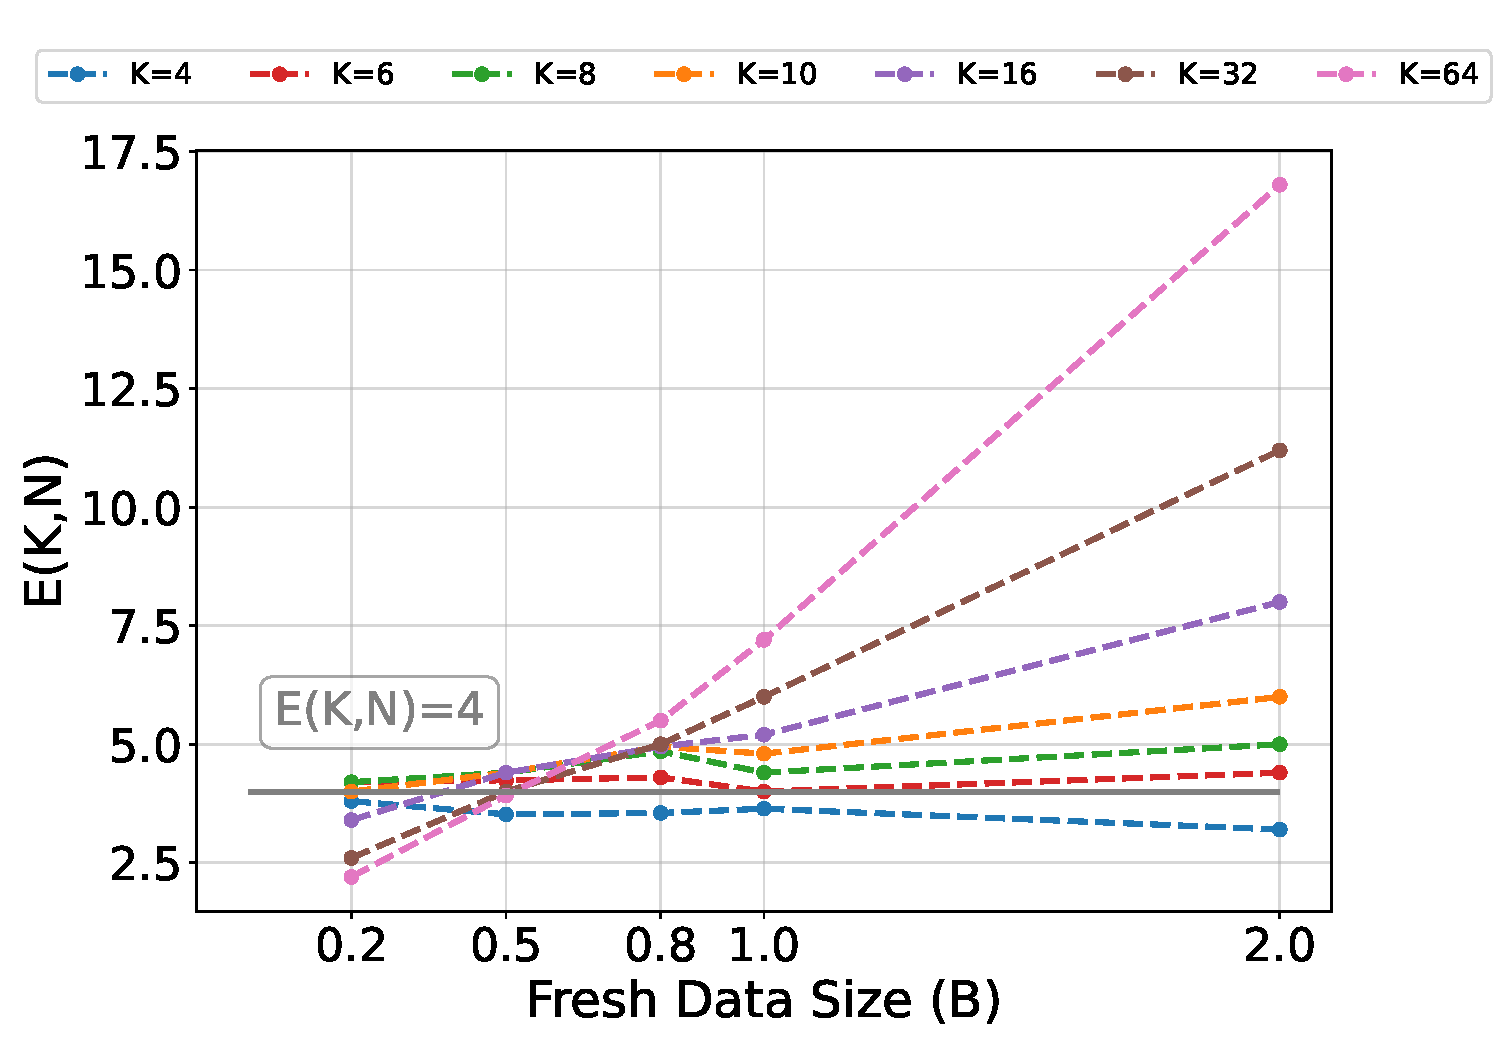
\includegraphics[width=0.6\linewidth]{figs/E_k_over_fresh_data_size.pdf}
    
%     \caption{The effective reuse rate $E(K,N)$ as a function of the fresh data size $N$.}\label{fig:ek-data}
% \end{figure}
%     % \includegraphics[width=\linewidth]{figures/LLM/loss_over_step.pdf}
%     % \caption{Training loss as a function of training steps for different fresh data sizes.}
%     % \label{fig:loss-step}

    
\begin{table}[htbp!]
\centering
\caption{Model configurations and parameter counts. $d_h$: hidden dimension; $d_f$: feed-forward dimension; $n_l$: number of Transformer layers; $n_h$: number of attention heads; $n_{kv}$: number of key-value heads (for grouped-query attention); Vocab Size: size of tokenizer vocabulary; \#NE params: number of non-embedding parameters (in millions); \#Params: total number of model parameters (in millions).}
\label{tab:model}
\begin{tabular}{lrrrrrrrrr}
\toprule
Name & $d_{h}$ & $d_f$ & $n_l$ & $n_h$ & $n_{kv}$ & Vocab Size & \#NE params & \#Params \\
\midrule
0.5B & 896 & 4864 & 24 & 14 & 2 & 151936 & 355 & 491 \\
0.3B & 640 & 3328 & 16 & 10 & 2 & 151936 & 117 & 331 \\
\bottomrule
\end{tabular}
\end{table}


\begin{table}[htbp!]
\centering
\caption{LLM Experiment Settings\label{tab:hyper}}
\begin{tabular}{ll}
\toprule
\textbf{Parameter} & \textbf{Value} \\
\midrule
\textbf{Data} & \\
\quad Sequence Batch Size & 128 \\
\quad Sequence Length & 4096 \\
\midrule
\textbf{Learning Rate} & \\
\quad Peak Learning Rate & 0.001 \\
\quad Schedule & Constant \\
\quad Warmup Steps & 400 \\
\midrule
\textbf{Optimizer} & \\
\quad Optimizer & AdamW \\
\quad Weight Decay & 0.1 \\
\quad $\beta_1$ & 0.9 \\
\quad $\beta_2$ & 0.95 \\
\quad $\epsilon$ & 1e-8 \\
\quad Gradient Clip & 1.0 \\
\bottomrule
\end{tabular}
\end{table}

% \section{Additional Experiments}\label{app:setup}

% In our pretraining experiments, we employ the AdamW optimizer with a weight decay of 0.1 and gradient clip of 1.0. We choose the peak learning rate as 0.001, around the optimal learning rate reported in~\citet{li2025predictablescalei}. We trade-off the optimal batch size according to~\citet{li2025predictablescalei} with the training efficiency, and use sequence batch size as 128, approximately 0.5M data each batch. Our pretraining model is approximately 117M when accounting non-embedding parameters conforming to~\citet{kaplan2020scaling} practice and 331M in total when following~\citet{hoffmann2022training} practice. Hyperparameter configurations are listed in \Cref{tab:hyper}, and detailed model architecture specifications are provided in \Cref{tab:model}. To ensure a fair comparison by eliminating the impact of batch order variations, we fix the random seed governing the data stream across all experiments. 

% \begin{table}[htbp!]
% \centering
% \caption{Model configurations and parameter counts. $d_h$: hidden dimension; $d_f$: feed-forward dimension; $n_l$: number of Transformer layers; $n_h$: number of attention heads; $n_{kv}$: number of key-value heads (for grouped-query attention); Vocab Size: size of tokenizer vocabulary; \#NE params: number of non-embedding parameters (in millions); \#Params: total number of model parameters (in millions).}
% \label{tab:model}
% \begin{tabular}{lrrrrrrrrr}
% \toprule
% Name & $d_{h}$ & $d_f$ & $n_l$ & $n_h$ & $n_{kv}$ & Vocab Size & \#NE params & \#Params \\
% \midrule
% 0.5B & 896 & 4864 & 24 & 14 & 2 & 151936 & 355M & 491M\\
% 0.3B & 640 & 3328 & 16 & 10 & 2 & 151936 & 117M & 331M\\
% \bottomrule
% \end{tabular}
% \end{table}


% \begin{table}[h!]

% \centering

% \caption{LLM Experiment Settings\label{tab:hyper}}

% \begin{tabular}{ll}

% \toprule

% \textbf{Parameter} & \textbf{Value} \\

% \midrule

% \textbf{Data} & \\

% \quad Sequence Batch Size & 128 \\

% \quad Sequence Length & 4096 \\

% \midrule

% \textbf{Learning Rate} & \\

% \quad Peak Learning Rate & 0.001 \\

% \quad Schedule & Constant \\

% \quad Warmup Steps & 400 \\

% \midrule

% \textbf{Optimizer} & \\

% \quad Optimizer & Adam \\

% \quad Weight Decay & 0.1 \\

% \quad $\beta_1$ & 0.9 \\

% \quad $\beta_2$ & 0.95 \\

% \quad $\epsilon$ & 1e-8 \\

% \quad Gradient Clip & 1.0 \\

% \bottomrule

% \end{tabular}

% \end{table}
\subsection{Fitting Experiments} \label{app:fitting experiments}
To provide real-world evidence that larger datasets can be repeated more, we show how the saturation points can be used to determine the appropriate number of training epochs. Recall that the saturation points are the points at which multi-epoch training first starts to underperform the one-pass baseline. We estimate these points from the pretraining loss curves presented in \Cref{sec:experiment-llm} and fit its dependence on $N$. 
% This fitted relationship provides an empirical rule for determining how many passes to use for a given dataset size: one can plug in this dataset size into the fitted formula and calculate $E(K,N)$. It represents a balance between training efficiency and low validation loss, thus its value is the suggested number of epochs.


To estimate this quantity from the training curves, we proceed as follows. First, to reduce the impact of noise, we smooth the loss curves with exponential moving average (EMA) with decay coefficient $\alpha = 0.9$ and a window size of 3 checkpoints. Then for each dataset size $N$, we examine the ratio $E(K,N)/K$. A larger ratio requires multi-epoch training to remain very close to the one-pass baseline, whereas a smaller ratio allows more deviation. Next, given a threshold hyperparameter $\lambda$, we identify the closest epoch $K$ at which this ratio first falls below $\lambda$, which we denote as $K(\lambda, N)$. Here we choose $\lambda = 0.75$, and we define $K(\lambda, N)$ as the saturation point.
% Finally, we take the corresponding $E(K,N)$ as the saturation point, and we denote this as $K(\lambda,N)$.

We fit those points and find that $K(\lambda,N)\approx 0.80\log N + 5.21$ with a correlation coefficient of $r=0.97$. The fitting results are shown in \Cref{fig:ek-n-saturation point}. 

% \subsection{Experiments on Learning Rate Schedule} \label{app:experiment-llm-lrs}
% Next, we conduct experiments to find how different learning rate schedules affect our experiment results. Here we select a $2$-stage learning rate schedule. Specifically, we first load checkpoints of our experiments with fresh dataset size 0.2B, 0.5B, 1B, 2B in \Cref{sec:experiment-llm} when trained for $2, 4, 8, 16$ epochs, and perform a linear learning rate decay from $10^{-3}$ to $10^{-5}$ for one epoch. For one-pass scenario, we take a learning rate schedule same as that of 2B. Then, for each dataset size, we fit the final loss after the decay, and fit a loss curve using the formula $y = A + \frac{B}{x^a}$. The fitted curves are used to predict the final loss after such a learning rate schedule. Finally, we use the curves to predict $E(K,N)$.

% Our results can be seen in \Cref{fig:ek-n-saturation-point-lrs}. We can see that under a different learning rate schedule, we still observe that $E(K,N) = \Theta(\log N)$. Specifically, we have $E(K,N)\approx 2.35\log N + 5.25$ with a coefficient of $0.96$. This shows that larger datasets can be repeated more under different learning rate schedules.
\begin{figure}[t]
    % \vspace{-0.4in}
    \centering
    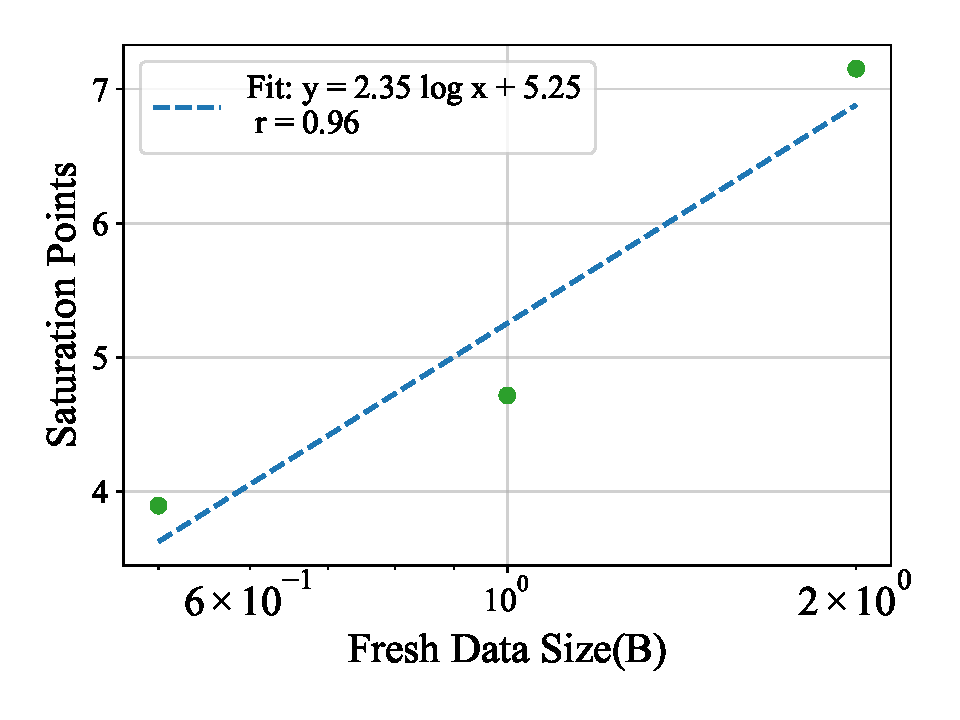
\includegraphics[width=0.5\linewidth]{figs/E_KN_vs_N_lrs.pdf}
    \caption{The saturation points $K(\lambda, N)$ as a function of the data size $N$ under a WSD learning rate schedule with linear decay.}
    \label{fig:ek-n-saturation-point-lrs}
\end{figure}
\subsection{Experiments with WSD Learning Rate Schedule}
\label{app:experiment-llm-lrs}

Next, to make our LLM experiments more consistent with real-world pretraining practices, we repeat the LLM experiments under a warmup-stable-decay(WSD) learning rate schedule.

Concretely, we start from the checkpoints obtained in \Cref{sec:experiment-llm} for fresh data sizes
$N \in \{0.2\text{B}, 0.5\text{B}, 1\text{B}, 2\text{B}\}$ after $K \in \{2,4,8,16\}$ epochs of pretraining with a constant learning rate of $10^{-3}$. From each checkpoint, we continue training for one additional epoch while linearly decaying the learning rate from $10^{-3}$ to $10^{-5}$, resulting in a WSD learning rate schedule followed by a linear decay. For the one-pass baseline, we adopt the same schedule as in the $N=2\text{B}$ run.

For each dataset size $N$, this process produces a set of four validation-loss values, each associated with one of the four selected epoch numbers $K$. We model the dependence of the final loss on the training steps $x$ using the parametric form  $\ell(x) = A + \frac{B}{x^{a}}$, where $A,B,a$ are fitted parameters. The fitted curves are then used to predict the final validation loss under this WSD schedule for arbitrary training budgets. Using these predictions, we compute the saturation points following the same procedure as in \Cref{sec:experiment-llm}. Here we still choose $\lambda = 0.75$.

The resulting saturation points are summarized in \Cref{fig:ek-n-saturation-point-lrs}. We observe that, even under this different learning rate schedule, the saturation points still satisfy the logarithmic scaling $K(\lambda,N) = \Theta(\log N).$ Specifically, we have $K(\lambda,N) \approx 2.35 \log N + 5.25$ with a correlation coefficient of $r = 0.96$. This confirms that our message that larger datasets can be repeated more also holds for real LLM training setups.


% \input{appendix_metamath_experiments}

\section{Additional Results and Simulations for Logarithmic Power-Law Spectrum}\label{app:log-spectrum}
\subsection{Scaling Law for Logarithmic Power-Law Spectrum}
We now present the scaling law for a logarithmic power-law spectrum.
% \kaifengclaw{Style: consider 'a logarithmic power-law spectrum' for grammar.} 
Its proof can be seen in \Cref{sec:proof-one-hot-scaling-law-log-spectrum}.
\begin{theorem} \label{thm:one-hot-log-scaling-law}
    Consider a $K$-epoch SGD over $N$ fresh data. Under Assumptions~\ref{asp:parameter-prior}, \Cref{asp:log-power-decay-prior}, and given the data dimension $d = \Omega((KN)^{\frac{1}{a}})$, it holds that
    \[
    \Bar{\cR}^*(K,N) \asymp 
    \begin{cases}
         \left(KN\right)^{-\frac{a-1}{a}} & \text{for } K = o(\log^b N) \\
         {\left(N\log^b N\right)^{-\frac{a-1}{a}}}& \text{for } K = \omega(\log^b N).
    \end{cases}
    \]
\end{theorem}

\subsection{Simulations in \Cref{sec:log-power-spectrum}}

Now we focus on validating the predictions of \Cref{thm:one-hot-E_K-log-spectrum} using synthetic data generated under the spectral assumptions of \Cref{sec:one_hot} and a log-power decay spectrum (\Cref{asp:log-power-decay-prior}).
% Because \Cref{thm:one-hot-loss-estimate} provides a closed-form expression for the multi-epoch loss in these settings, we can perform a more controlled simulation of $E(K,N)$. In particular, we consider two cases: (i) a power-law decay Hessian spectrum (\Cref{asp:prior-probability-and-norm}), and (ii) a log-power decay spectrum (\Cref{asp:log-power-decay-prior}), corresponding to the conditions of \Cref{thm:one-hot-E_K-v2} and \Cref{thm:one-hot-E_K-log-spectrum}, respectively.

\paragraph{Experiments Setup.} Similar to \Cref{sec:power-spectrum-experiment}, in all sub-figures of \Cref{fig:one-hot-log}, we set the data dimension $d$ to $10^5$ and tune all the learning rates to their optimal values. Here we set $a=1.5$ and $b=2$. 
% In the simulations of the power spectrum case, we 
% \paragraph{Simulations in Power Spectrum Case.} 
% The top-left panel of \Cref{fig:one-hot-log} plots $E(K,N)$ versus $\log K$ for various fixed $N$, while the right panels show $E(K,N)$ versus $\log N$ for various fixed $K$. In the power-law spectrum scenario, we observe an initial regime where $E(K,N)$ increases almost linearly with $K$ (indicating that more epochs initially provide almost proportional gains in effective data usage), followed by a clear saturation regime where $E(K,N)$ approaches a constant plateau even as $K$ continues to grow. This plateau value is much lower than $K$ when $K$ is large, and it depends on $N$ in a manner consistent with our theory. Specifically, $E(K,N)$ eventually saturates at an asymptotic value, and larger datasets yield higher saturation levels, reflecting a dataset-dependent multiple-epoch benefit, as predicted by \Cref{thm:one-hot-E_K-v2}.  

% % \begin{figure}[htbp]
% % \begin{figure}[t!]
% %     \centering
% %     \includegraphics[width=0.6\linewidth]{figures/one-hot-simulation/E_K_comparison_2x2_paper.pdf}
% %     \caption{Simulation results in the solvable case with power law. \textbf{Top-Left:}}
% %     \label{fig:one-hot-log}
% % \end{figure}

% \paragraph{Simulations in Log-Power Spectrum Case.} 
% In the log-power spectrum setting (bottom panels of \Cref{fig:one-hot-log}), $E(K,N)$ exhibits a similar two-regime behavior: the initial growth with $K$ transitions to a plateau whose height increases only logarithmically with $N$ (on the order of $\log^b N$), as described by \Cref{thm:one-hot-E_K-log-spectrum}. The curves depicting $E(K,N)$ versus $\log N$ further illustrate that, for fixed small values of $K$, increasing $N$ eventually yields diminishing returns as $E(K,N)$ approaches the $K$ limit (analogous to the strongly-convex case). For larger values of $K$, however, the effective multiplier reaches a ceiling determined by the dataset-dependent saturation value. These experiments demonstrate the anticipated saturation effects, multiple scaling regimes, and asymptotic plateaus, providing empirical confirmation of the scaling behaviors predicted by \Cref{thm:one-hot-E_K-v2} and \Cref{thm:one-hot-E_K-log-spectrum}.




\paragraph{Simulations for the Solvable Model.} \Cref{fig:one-hot-log} plots $E(K, N)$ versus $K$ and $\log N$ for the solvable model. The curves depicting $E(K,N)$ versus $K$ and $E(K,N)$ versus $\log N$ show trends consistent with those in \Cref{sec:power-spectrum-experiment}, aligning with \Cref{thm:one-hot-E_K-log-spectrum}. 
% The top line and the bottom line show the plots in power spectrum case and log-power spectrum case respectively. For both cases, the curves depicting $E(K,N)$ versus $K$ show that $E(K,N)\approx K$ when $K$ is relatively small and saturate to some value depending on $N$ when $K$ is large. In the right panels, which describe the relationship between $E(K,N)$ and $\log N$, we observe that when $K$ is small (namely $K=2$), $E(K,N)$ increases and approaches $K$ as $\log N$ increases, and the plots overlap when $K$ is large. Those pheomena provide empirical confirmation of the scaling behaviors predicted by \Cref{thm:one-hot-E_K-v2} and \Cref{thm:one-hot-E_K-log-spectrum}. 
Furthermore, in the large-$K$ regime, we fit the exponent according to \Cref{thm:one-hot-E_K-log-spectrum} and obtain $2.036 \approx b = 2$, which provides strong validation of our theory.


% We now verify the predictions of \Cref{thm:one-hot-E_K-v2} and \Cref{thm:one-hot-E_K-log-spectrum} using synthetic data generated under the spectral assumptions of \Cref{sec:one_hot}. Because \Cref{thm:one-hot-loss-estimate} provides a closed-form expression for the multi-epoch loss in these settings, we can perform a more controlled simulation of $E(K,N)$. In particular, we consider two cases: (i) a power-law decay Hessian spectrum (\Cref{asp:prior-probability-and-norm}), and (ii) a log-power decay spectrum (\Cref{asp:log-power-decay-prior}), corresponding to the conditions of \Cref{thm:one-hot-E_K-v2} and \Cref{thm:one-hot-E_K-log-spectrum}, respectively.

% \paragraph{Experiments Setup.} In all sub-figures of \Cref{fig:one-hot-log}, we set the data dimension $d$ to $10^5$ and tune all the learning rates to their optimal values. Additionally, we separately tune the spectrum parameters $a$ and $b$ in each sub-figure of \Cref{fig:one-hot-log}. Specifically, in the top-left and top-right panels, we set $a=4.5$ and $b=1$, whereas in the bottom-left and bottom-right panels, we set $a=1.5$ and $b=2$. 
% % In the simulations of the power spectrum case, we 
% % \paragraph{Simulations in Power Spectrum Case.} 
% % The top-left panel of \Cref{fig:one-hot-log} plots $E(K,N)$ versus $\log K$ for various fixed $N$, while the right panels show $E(K,N)$ versus $\log N$ for various fixed $K$. In the power-law spectrum scenario, we observe an initial regime where $E(K,N)$ increases almost linearly with $K$ (indicating that more epochs initially provide almost proportional gains in effective data usage), followed by a clear saturation regime where $E(K,N)$ approaches a constant plateau even as $K$ continues to grow. This plateau value is much lower than $K$ when $K$ is large, and it depends on $N$ in a manner consistent with our theory. Specifically, $E(K,N)$ eventually saturates at an asymptotic value, and larger datasets yield higher saturation levels, reflecting a dataset-dependent multiple-epoch benefit, as predicted by \Cref{thm:one-hot-E_K-v2}.  

% % % \begin{figure}[htbp]
% % % \begin{figure}[t!]
% % %     \centering
% % %     \includegraphics[width=0.6\linewidth]{figures/one-hot-simulation/E_K_comparison_2x2_paper.pdf}
% % %     \caption{Simulation results in the solvable case with power law. \textbf{Top-Left:}}
% % %     \label{fig:one-hot-log}
% % % \end{figure}

% % \paragraph{Simulations in Log-Power Spectrum Case.} 
% % In the log-power spectrum setting (bottom panels of \Cref{fig:one-hot-log}), $E(K,N)$ exhibits a similar two-regime behavior: the initial growth with $K$ transitions to a plateau whose height increases only logarithmically with $N$ (on the order of $\log^b N$), as described by \Cref{thm:one-hot-E_K-log-spectrum}. The curves depicting $E(K,N)$ versus $\log N$ further illustrate that, for fixed small values of $K$, increasing $N$ eventually yields diminishing returns as $E(K,N)$ approaches the $K$ limit (analogous to the strongly-convex case). For larger values of $K$, however, the effective multiplier reaches a ceiling determined by the dataset-dependent saturation value. These experiments demonstrate the anticipated saturation effects, multiple scaling regimes, and asymptotic plateaus, providing empirical confirmation of the scaling behaviors predicted by \Cref{thm:one-hot-E_K-v2} and \Cref{thm:one-hot-E_K-log-spectrum}.

% \paragraph{Simulations for the Solvable Model.} \Cref{fig:one-hot-log} plots $E(K, N)$ versus $K$ and $\log N$ for the solvable model. The top line and the bottom line show the plots in power spectrum case and log-power spectrum case respectively. For both cases, the curves depicting $E(K,N)$ versus $K$ show that $E(K,N)\approx K$ when $K$ is relatively small and saturate to some value depending on $N$ when $K$ is large. In the right panels, which describe the relationship between $E(K,N)$ and $\log N$, we observe that when $K$ is small (namely $K=2$), $E(K,N)$ increases and approaches $K$ as $\log N$ increases, and the plots overlap when $K$ is large. Those pheomena provide empirical confirmation of the scaling behaviors predicted by \Cref{thm:one-hot-E_K-v2} and \Cref{thm:one-hot-E_K-log-spectrum}. We also fit exponents base on \Cref{thm:one-hot-E_K-v2} and \Cref{thm:one-hot-E_K-log-spectrum} in large-$K$ regime. In the power-spectrum case, the fitted exponent is $0.279 \approx \tfrac{b}{a-b} = \tfrac{2}{7}$, while in the log-spectrum case, the fitted exponent is $2.036 \approx b = 2$, perfectly validating our theory.


% We now verify the predictions of \Cref{thm:one-hot-E_K-log-spectrum} using synthetic data generated under the spectral assumptions of \Cref{sec:one_hot} 
% % Because \Cref{thm:one-hot-loss-estimate} provides a closed-form expression for the multi-epoch loss in these settings, we can perform a more controlled simulation of $E(K,N)$. 
% % In particular, we consider two cases: (i) 
% with a power-law decay Hessian spectrum (\Cref{asp:prior-probability-and-norm}).


% % We now verify the predictions of \Cref{thm:one-hot-E_K-log-spectrum} using synthetic data generated under the spectral assumptions of \Cref{sec:one_hot} 
% % % Because \Cref{thm:one-hot-loss-estimate} provides a closed-form expression for the multi-epoch loss in these settings, we can perform a more controlled simulation of $E(K,N)$. 
% % % In particular, we consider two cases: (i) 
% % with a power-law decay Hessian spectrum (\Cref{asp:prior-probability-and-norm}).

% % % , and (ii) a log-power decay spectrum (\Cref{asp:log-power-decay-prior}), corresponding to the conditions of \Cref{thm:one-hot-E_K-v2} and \Cref{thm:one-hot-E_K-log-spectrum}, respectively.

% % \paragraph{Experiments Setup.} In all sub-figures of \Cref{fig:one-hot-log}, we set the data dimension $d$ to $10^5$ and tune all the learning rates to their optimal values. Here we set $a=1.5$ and $b=2$. 

% % % . Additionally, we separately tune the spectrum parameters $a$ and $b$ in each sub-figure of \Cref{fig:one-hot-log}. Specifically, in the top-left and top-right panels, we set $a=4.5$ and $b=1$, whereas in the bottom-left and bottom-right panels, we set $a=1.5$ and $b=2$. 
% % % In the simulations of the power spectrum case, we 
% % % \paragraph{Simulations in Power Spectrum Case.} 
% % % The top-left panel of \Cref{fig:one-hot-log} plots $E(K,N)$ versus $\log K$ for various fixed $N$, while the right panels show $E(K,N)$ versus $\log N$ for various fixed $K$. In the power-law spectrum scenario, we observe an initial regime where $E(K,N)$ increases almost linearly with $K$ (indicating that more epochs initially provide almost proportional gains in effective data usage), followed by a clear saturation regime where $E(K,N)$ approaches a constant plateau even as $K$ continues to grow. This plateau value is much lower than $K$ when $K$ is large, and it depends on $N$ in a manner consistent with our theory. Specifically, $E(K,N)$ eventually saturates at an asymptotic value, and larger datasets yield higher saturation levels, reflecting a dataset-dependent multiple-epoch benefit, as predicted by \Cref{thm:one-hot-E_K-v2}.  

% % % % \begin{figure}[htbp]
% % % % \begin{figure}[t!]
% % % %     \centering
% % % %     \includegraphics[width=0.6\linewidth]{figures/one-hot-simulation/E_K_comparison_2x2_paper.pdf}
% % % %     \caption{Simulation results in the solvable case with power law. \textbf{Top-Left:}}
% % % %     \label{fig:one-hot-log}
% % % % \end{figure}

% % % \paragraph{Simulations in Log-Power Spectrum Case.} 
% % % In the log-power spectrum setting (bottom panels of \Cref{fig:one-hot-log}), $E(K,N)$ exhibits a similar two-regime behavior: the initial growth with $K$ transitions to a plateau whose height increases only logarithmically with $N$ (on the order of $\log^b N$), as described by \Cref{thm:one-hot-E_K-log-spectrum}. The curves depicting $E(K,N)$ versus $\log N$ further illustrate that, for fixed small values of $K$, increasing $N$ eventually yields diminishing returns as $E(K,N)$ approaches the $K$ limit (analogous to the strongly-convex case). For larger values of $K$, however, the effective multiplier reaches a ceiling determined by the dataset-dependent saturation value. These experiments demonstrate the anticipated saturation effects, multiple scaling regimes, and asymptotic plateaus, providing empirical confirmation of the scaling behaviors predicted by \Cref{thm:one-hot-E_K-v2} and \Cref{thm:one-hot-E_K-log-spectrum}.

% % \paragraph{Simulations for the Solvable Model.} \Cref{fig:one-hot-log} plots $E(K, N)$ versus $K$ and $\log N$ for the solvable model. The curves depicting $E(K,N)$ versus $K$ show that $E(K,N)\approx K$ when $K$ is relatively small and saturate to some value depending on $N$ when $K$ is large. In the right panel, which describe the relationship between $E(K,N)$ and $\log N$, we observe that when $K$ is small (namely $K=2$), $E(K,N)$ increases and approaches $K$ as $\log N$ increases, and the plots overlap when $K$ is large. Those pheomena provide empirical confirmation of the scaling behaviors predicted by \Cref{thm:one-hot-E_K-v2}. We also fit exponents based on \Cref{thm:one-hot-E_K-v2} in the large-$K$ regime. In the power-spectrum case, the fitted exponent is $0.279 \approx \tfrac{b}{a-b} = \tfrac{2}{7}$, perfectly validating our theory.
% % % \vspace{-0.4mm}
% We now verify the predictions of \Cref{thm:one-hot-E_K-v2} and \Cref{thm:one-hot-E_K-log-spectrum} using synthetic data generated under the spectral assumptions of \Cref{sec:one_hot}. Because \Cref{thm:one-hot-loss-estimate} provides a closed-form expression for the multi-epoch loss in these settings, we can perform a more controlled simulation of $E(K,N)$. In particular, we consider two cases: (i) a power-law decay Hessian spectrum (\Cref{asp:prior-probability-and-norm}), and (ii) a log-power decay spectrum (\Cref{asp:log-power-decay-prior}), corresponding to the conditions of \Cref{thm:one-hot-E_K-v2} and \Cref{thm:one-hot-E_K-log-spectrum}, respectively.
\begin{figure}[t!]
    % \vspace{-0.7in}
    \centering
    % \begin{subfigure}[b]{0.98\linewidth} 
    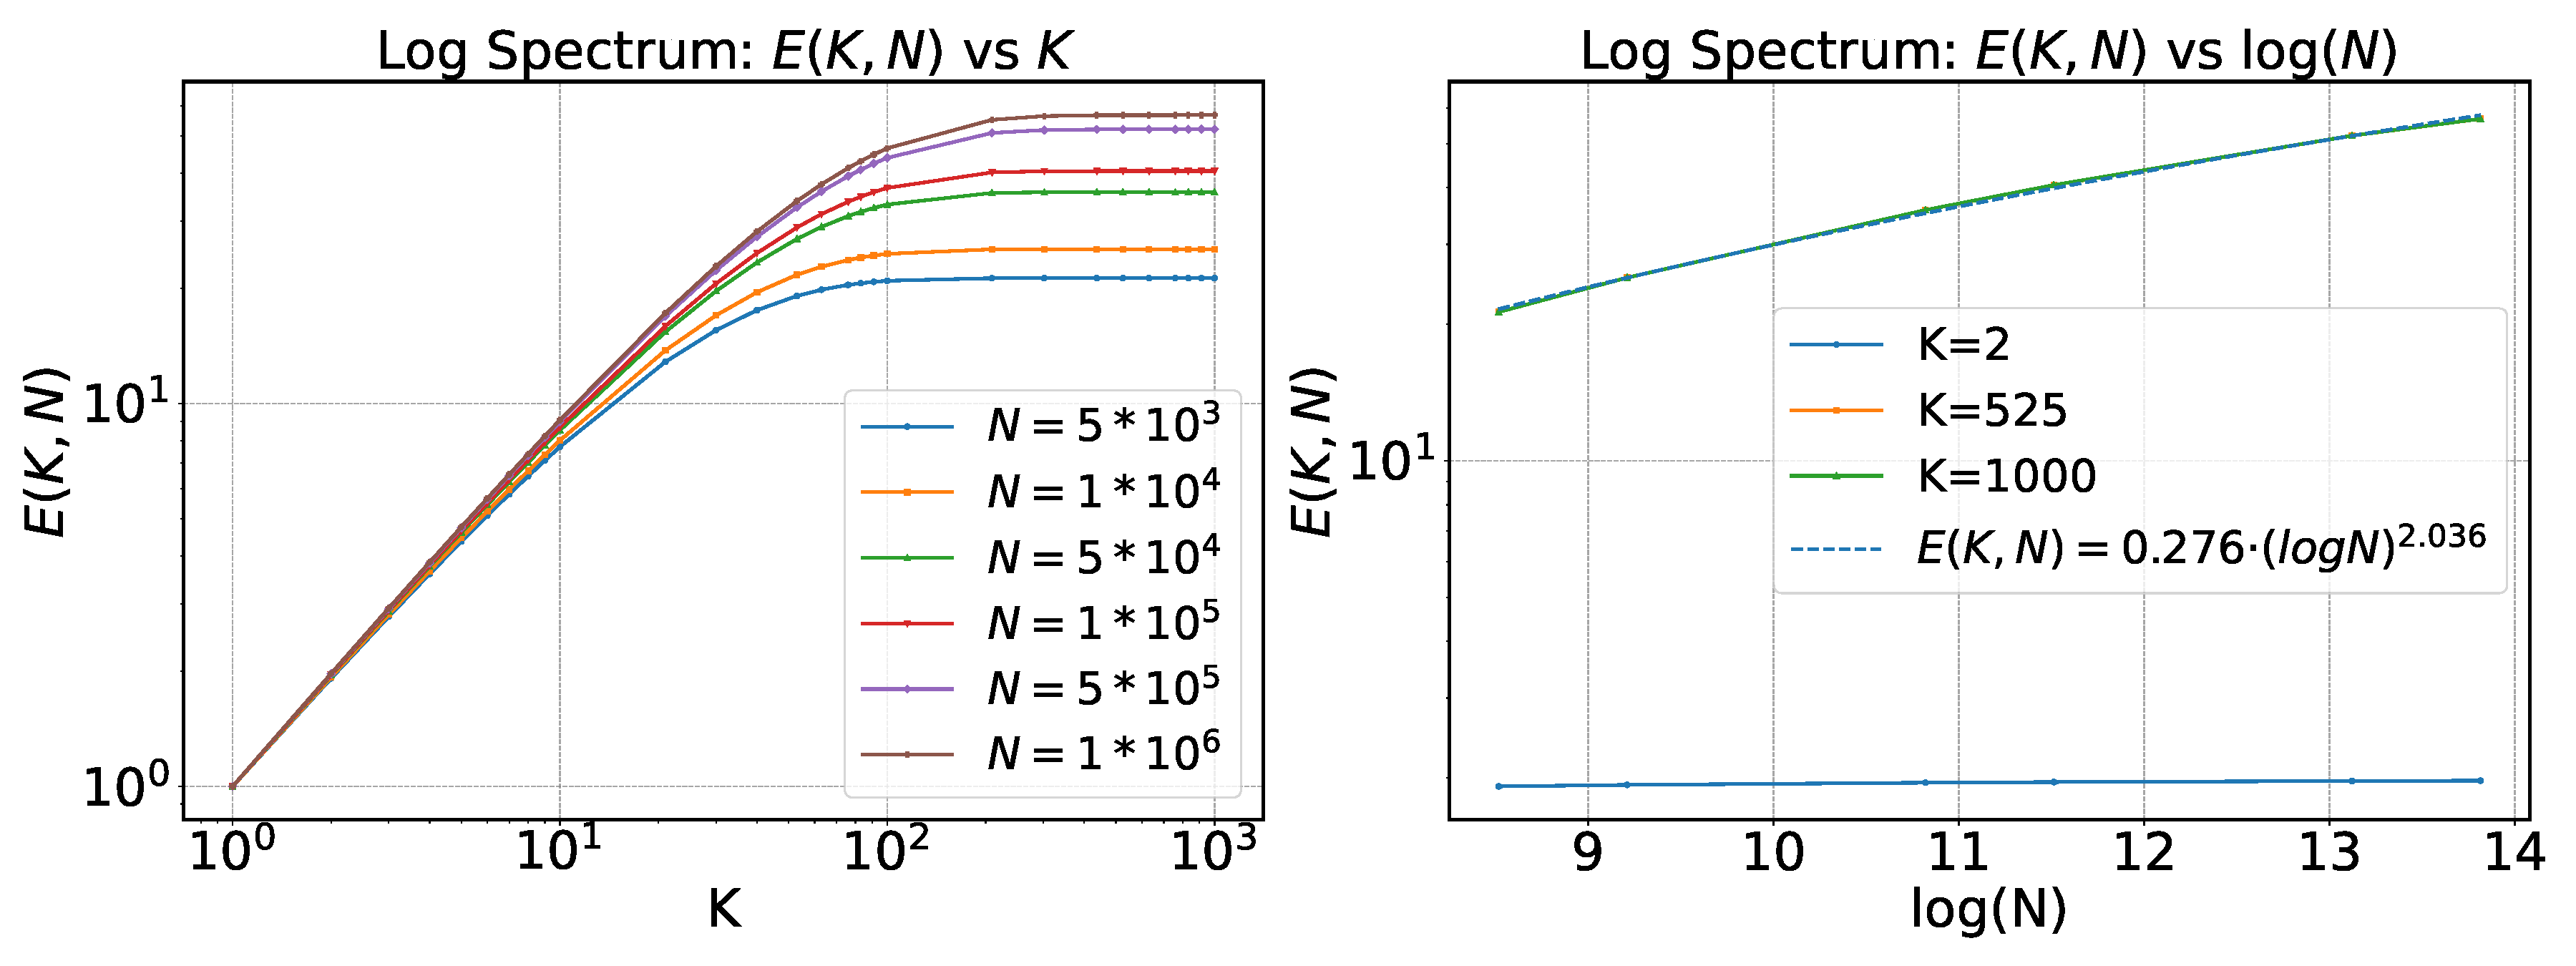
\includegraphics[width=\linewidth]{figs/E_K_comparison_log.pdf}
         \caption{The solvable cases with logarithmic power-law spectrum. $E(K,N)$ exhibits a similar behavior to that presented in \Cref{fig:convex-and-power}. We also fit the effective reuse rate using the formula $E(K,N)=c_1\left(\log N\right)^{c_2}$ suggested by \Cref{thm:one-hot-E_K-log-spectrum}, and the fitted exponent $c_2=2\approx b=2$ matches our theory.}
         % \kaifengclaw{Reference logic: this log-spectrum fit is more directly tied to \Cref{thm:one-hot-E_K-log-spectrum}; consider citing that theorem here.}
        % \caption{The effective reuse rate $E(K,N)$ as a function of the number of training epochs $K$ for varying fresh data sizes $N$. The shaded regions represent the variability from the smoothed trend in different epochs.}
        \label{fig:one-hot-log}
    % \end{subfigure}   
\end{figure}

    \section{Additional Notations}\label{app:notation}
% \begin{align*}
%     &\pi_k ~\text{denotes the permutation in the i-th epoch.} \\
%     &\mA^{(k)}:=(\mI -\eta \vx_{\pi_k(N-1)}\vx_{\pi_k(N-1)}^{\top})\cdots(\mI -\eta \vx_{\pi_k(0)}\vx_{\pi_k(0)}^{\top}) \\
%     &\forall k, \E\mA^{(k)}:=\E\mA = (\mI-\eta\mH)^{N} \\
%     &\mZ^{(k)}_{a \to b} := (\mI -\eta \vx_{\pi_k(a)}\vx_{\pi_k(a)}^{\top})\cdots(\mI -\eta \vx_{\pi_k(b)}\vx_{\pi_k(b)}^{\top}),~~\text{Specifically, $\mA^{(k)} = \mZ^{(k)}_{N-1 \to 0}$}\\
%     &\text{always use }~~K ~~\text{instead of}~~k~~\\ 
%     &\mT^{(k)}:=\mA^{(K)}\cdots\mA^{(k+1)} ~\text{and} ~\mT^{(K)} = \mI \\
%     &\fakeE\mT^{(k)}:=(\mI-\eta\mH)^{K-1-k} \\
%     &\fakeE S_{0 \to k-1}(\mA) := \mI + \E[\mA] + \E[\mA]^2 + \dots + \E[\mA]^{k-1}\\
%     &\mS_{0 \to k-1} := \mI+\mA+\cdots+\mA^{k-1}\\
%     &\mS_l^{(ij)} := \mZ_{N-1 \to \pi_i(l)+1}^{(i)}\vx_l\vx_l^{\top} \mZ_{\pi_j(l)+1 \to N-1}^{(j)}\\
%     &\fakeE \mS_l^{(ij)}:=\fakeE \mS_l^{(ij)} \\
%     &\mS^{(ij)} := \sum_{l=0}^{N-1}\mS_l^{(ij)} \\
%     &\vb^{(k)} := \eta \sum_{l=0}^{N-1}(\mI -\eta \vx_{\pi_k(N-1)}\vx_{\pi_k(N-1)}^{\top})\cdots(\mI -\eta \vx_{\pi_k(l+1)}\vx_{\pi_k(l+1)}^{\top})\xi_{\pi_k(l)}\vx_{\pi_k(l)} \\
%     &= \eta \sum_{l=0}^{N-1}(\mI -\eta \vx_{\pi_k(N-1)}\vx_{\pi_k(N-1)}^{\top})\cdots(\mI -\eta \vx_{\pi_k(\pi_k^{-1}(l)+1)}\vx_{\pi_k(\pi_k^{-1}(l)+1)}^{\top})\xi_{l}\vx_{l} \\
%     &\text{\tingkai{We need to modify the definition of $\mZ^{(k)}_{a \to b}$.}} \\
%     &\mS_{1 \to k-1} := \mA+\cdots+\mA^{k-1} = \mS_k~~~\text{for short}\\
%     &\mS_{i \to j}(\mA):=\mA^{i}+\cdots+\mA^{j}\\
%     & \prod_{l=j}^i \mA^{(l)}:= \mA^{(j)}\mA^{(j-1)}\cdots\mA^{(i)}\;for\;i\le j. \\
%     &\Tilde{\mA}:=\mS\mA\mS^{\top} \text{for a matrix} \mA.
% \end{align*}
% \begin{align*}
%     &\mA^{(k)}:=(\mI -\eta \vx_{\pi_k(N-1)}\vx_{\pi_k(N-1)}^{\top})\cdots(\mI -\eta \vx_{\pi_k(0)}\vx_{\pi_k(0)}^{\top}) \\
%     &\mZ^{(k)}_{a \to b} := (\mI -\eta \vx_{\pi_k(a)}\vx_{\pi_k(a)}^{\top})\cdots(\mI -\eta \vx_{\pi_k(b)}\vx_{\pi_k(b)}^{\top}),~~\text{Specifically, $\mA^{(k)} = \mZ^{(k)}_{N-1 \to 0}$.}\\
%     &\mT^{(k)}:=\mA^{(K)}\cdots\mA^{(k+1)} ~\text{and} ~\mT^{(K)} = \mI. \\
%     &\mS_l^{(ij)} := \mZ_{N-1 \to \pi_i^{-1}(l)+1}^{(i)}\vx_l\vx_l^{\top} \mZ_{\pi_j^{-1}(l)+1 \to N-1}^{(j)}\\
%     &\vb^{(k)} := \eta \sum_{l=0}^{N-1}(\mI -\eta \vx_{\pi_k(N-1)}\vx_{\pi_k(N-1)}^{\top})\cdots(\mI -\eta \vx_{\pi_k(l+1)}\vx_{\pi_k(l+1)}^{\top})\xi_{\pi_k(l)}\vx_{\pi_k(l)} \\
%     &= \eta \sum_{l=0}^{N-1}(\mI -\eta \vx_{\pi_k(N-1)}\vx_{\pi_k(N-1)}^{\top})\cdots(\mI -\eta \vx_{\pi_k(\pi_k^{-1}(l)+1)}\vx_{\pi_k(\pi_k^{-1}(l)+1)}^{\top})\xi_{l}\vx_{l} \\
% \end{align*}
In this section, we provide some additional notations appeared in the following proof of our main results.

\paragraph{Key Quantities.} We define the following key quantities to analyze the sequential updates. For each epoch $k$, let 
\begin{equation}
    \mA^{(k)} := \prod_{i= N-1}^0 (\mI - \eta \vx_{\pi_k(i)}\vx_{\pi_k(i)}^{\top})\label{app:A_def}
\end{equation}
represent the product of sequential updates through all samples in epoch $k$. More generally, we define the partial product operator:
\begin{align*}
    \mZ^{(k)}_{a \to b} &:= \prod_{i=a}^b(\mI - \eta \vx_{\pi_k(i)}\vx_{\pi_k(i)}^{\top}), \quad \text{with} \quad \mA^{(k)} = \mZ^{(k)}_{N-1 \to 0}.
\end{align*}
We further define that $\mZ^{(k)}_{N-1 \to N} = \mI$. The cumulative effect across epochs is captured by:
\begin{align*}
    \mT^{(k)} &:= \prod_{i=K}^{k+1}\mA^{(i)}, \quad \text{and} \quad \mT^{(K)} = \mI.
\end{align*}
% For analyzing the specific contribution of each sample, we define:
% \begin{align*}
%     \mS_l^{(ij)} &:= \mZ_{N-1 \to \pi_i^{-1}(l)+1}^{(i)}\vx_l\vx_l^{\top} \mZ_{\pi_j^{-1}(l)+1 \to N-1}^{(j)},
% \end{align*}
% which isolates the effect of sample $l$ between epochs $i$ and $j$. The accumulation term of noise is given by:
% \begin{align*}
%     \vb^{(k)} &:= \eta \sum_{l=0}^{N-1} (\mI - \eta \vx_{\pi_k(N-1)}\vx_{\pi_k(N-1)}^{\top}) \cdots (\mI - \eta \vx_{\pi_k(l+1)}\vx_{\pi_k(l+1)}^{\top}) \xi_{\pi_k(l)}\vx_{\pi_k(l)} \\
%     &= \eta \sum_{l=0}^{N-1} (\mI - \eta \vx_{\pi_k(N-1)}\vx_{\pi_k(N-1)}^{\top}) \cdots (\mI - \eta \vx_{\pi_k(\pi_k^{-1}(l)+1)}\vx_{\pi_k(\pi_k^{-1}(l)+1)}^{\top}) \xi_{l}\vx_{l},
% \end{align*}
% representing the propagated noise contribution through the update sequence.
% We define a constant $\deltaA:= \Tilde{C}8eD^4\log d$, which is independent of training time $T$ and learning rate $\eta$, and $\Tilde{C}$ is some absolute constant stated in \Cref{lem:un-shuffle-A-EA-expectation}.

\paragraph{Pseudo-expectation Notation $\fakeE$.} Because matrix multiplication is non-commutative and the shuffling in training introduces statistical dependence, the expectations of the random matrices defined above cannot be written in a tractable closed form. To approximate the population excess risk, we therefore introduce the auxiliary notation $\fakeE$.  By construction, $\fakeE$ computes the expectation of each factor as if the variables were independent, deliberately neglecting the correlations.  We then invoke matrix-concentration inequalities to bound the gap between this ``pseudo''-expectation and the true expectation of the original dependent random variables. Specifically, for the above random matrices used in our proof, here we further define that
\begin{align}
  \fakeE\mZ_{a \to b}^{(k)}
    &:= (\mI - \eta \mH)^{a-b+1},\\
  \fakeE\mA^{(k)}
    &:= (\mI - \eta \mH)^{N},\\
  \fakeE\mT^{(k)}
    &:= (\mI - \eta \mH)^{N(K-k)},\label{equ:faek-T}\\
  \fakeE\mS_l^{(ij)}
    &:= \fakeE\!\Bigl[\mZ_{N-1 \to \pi_i^{-1}(l)+1}^{(i)}\Bigr]\,
        \E\!\bigl[\vx_l\vx_l^{\top}\bigr]\,
        \fakeE\!\Bigl[\mZ_{\pi_j^{-1}(l)+1 \to N-1}^{(j)}\Bigr]. \label{equ:faek-S}
\end{align}



% In general, for a random matrix $\mM:=\sum_{i}\prod_{j}^{f(i)}{\mM_{ij}}$, where $\mM_{ij}$ we define 
% \begin{align*}
%     \fakeE\mM:=\sum_{i}\prod_{j}^{f(i)}\E{\mM_{ij}}
% \end{align*}
% to be the fake expectation of $\mB$, which is an approximation of $\E\mB$. 

%\input{appendix_strongly_conv_tech_challenge}

\section{Proof Outline in Strongly Convex Linear Regression}\label{sec:convex-proof-outline}
In this section, we give the outline of \Cref{thm:convex-L-estimate}, \Cref{thm:convex-opt-lr}, and \Cref{thm:convex-E_K}. The main technical challenges and our proof insights are briefly stated in \Cref{sec:strongly-convex-tech}.

\Cref{sec:strongly_convex} centres on \Cref{thm:convex-E_K}, which establishes a scaling law for the effective reuse rate $E(K,N)$ in terms of the relative magnitudes of number of epochs $K$ and dataset size $N$. Its proof unfolds in three stages.

\paragraph{1. An explicit approximation of the expected excess risk.} \Cref{thm:convex-L-estimate} derives a sufficiently accurate asymptotic formula for the expected excess risk of multi-epoch SGD. The argument begins with a bias–variance decomposition, splitting the expected excess risk into a variance term (\Cref{lem:variance-estimate}) and a bias term (\Cref{lem:bias-estimate}).
\begin{itemize}
    \item \textbf{Variance term.} The closed-form approximation relies on concentration properties of matrix contractions together with a careful treatment of data shuffling.
    \item \textbf{Bias term.} The same contraction inequality is employed to obtain an analytic expression, after which tight error bounds are proved for the full range of relative sizes of $K$ and $N$. These bounds hold uniformly over a broad class of learning rates, necessitating detailed case-by-case analysis.
\end{itemize}

\paragraph{2. Selection of a nearly optimal learning rate.}
\Cref{thm:convex-opt-lr} identifies a learning rate whose resulting loss is asymptotically equivalent to the minimum excess risk attained with the optimal learning rate as stated in \Cref{sec:setup}. This ``approximately optimal learning rate'' will be fixed in Appendix~\ref{proof:convex-opt-lr}.

\paragraph{3. Proof of the effective reuse rate scaling law.} With the one-pass and multi-epoch SGD training learning rate set to the near-optimal learning rate obtained above, the proof of \Cref{thm:convex-E_K} proceeds to characterise the behaviour of $E(K,N)$ as $K$ and $N$ vary, yielding the desired scaling relation.
Together, these three components establish \Cref{thm:convex-E_K} and provide a comprehensive description of how reuse efficiency depends on the interplay between $K$ and $N$.

\section{Proof of Main Results in Strongly Convex Linear Regression}\label{sec:proof-convex}

% \haodong{we have no $R^{var}$ or $R^{bias}$ in the main context!!}
\subsection{Step I: A Concrete Version of Bias-Variance Decomposition}
Before we begin our proof, we first present the following lemma, which provides the formal version of the loss estimate for a specific range of learning rate parameters. We define a $\widehat{\cR}(K,N, \eta)$ as the estimator of $\Bar{\cR}(K,N;\eta)$ 
\begin{align*}
    \widehat{\cR}(K,N;\eta)&:= \underbrace{\widehat{\cR}_1(K,N; \eta)}_{\textit{bias term}} + \underbrace{ \widehat{\cR}_2(K,N; \eta)}_{\textit{var term across epochs}} + \underbrace{ \widehat{\cR}_3(K,N;\eta)}_{\textit{var term within epoch}},
\end{align*}
where
\begin{align*}
    \widehat{\cR}_1(K,N;\eta) := \frac{1}{2}(\vw_0 - \vw^*)^{\top} (\mI-\eta\mH)^{2KN}\mH (\vw_0 - \vw^*),
\end{align*}
\begin{align*}
    \widehat{\cR}_2(K,N;\eta) := \frac{\sigma^2}{N} tr\left(\frac{\left(\mI -(\mI -\eta\mH)^{KN}\right)\left((\mI -\eta\mH)^{N} -(\mI -\eta\mH)^{KN}\right)}{\mI + (\mI -\eta\mH)^N}\right),
\end{align*}
\begin{align*}
    \widehat{\cR}_3(K,N;\eta) :=  \frac{\eta\sigma^2}{2}\inp{\mH}{(\mI - (\mI - \eta \mH)^{2KN})(2\mI-\eta\mH)^{-1}}.
\end{align*}
\subsection{Step II: Risk Approximation and Error Bound Analysis}\label{sec:proof-thm-convex-L-estimate}
In this section, we rigorously formulate the analytic risk approximation in \Cref{thm:convex-L-estimate} and provide its proof. \Cref{thm:convex-L-estimate} indicates that the error bound is of higher order than the main term when the parameters are restricted to a limited range of values.
\begin{lemma}\label{thm:convex-L-estimate}
    Under \Cref{asp:strongly-convex} and \ref{asp:large-dataset}, we further assume that for every $\vx$ in the training set, $\|\vx\| \leq D$ for some constant $D>0$. Consider a $K$-epoch SGD with learning rate $\eta \in \left[\Omega\left(\frac{1}{T}\right), o(T^{-\frac{3}{4}})\right]$, $K = o\left(\eta^{-1} T^{-\frac{3}{4}}\right)$ and data shuffling. Then, after $T = KN$ steps, the estimator of the expected excess risk satisfies:
    \begin{align*}
        \Bar{\cR}(K,N;\eta) = \widehat{\cR}(K,N; \eta)\left(1+o(1)\right).
    \end{align*}
\end{lemma}

% \haodong{in lack of more evidence for this decomposition. May be very confusing here.}
Recall from \Cref{step:bias-var-decomposition} that the risk $\Bar{\cR}(K,N;\eta)$ can be decomposed into the \textit{bias term} $\Bar{\cR}^{\bias}(K,N;\eta):= \frac{1}{2}\left\|\vtheta_t^{\bias}\right\|_{\mH}^2$ and \textit{variance term} $\Bar{\cR}^{\var}(K,N;\eta):=\frac{1}{2}\left\|\vtheta_t^{\var}\right\|_{\mH}^2$, which implies that \Cref{thm:convex-L-estimate} is a direct corollary of the following two lemmas:
\begin{lemma}[Variance Term] \label{lem:variance-estimate}
    Suppose that \Cref{asp:strongly-convex} holds. Then for a $K$-epoch SGD with dataset size $N$ and learning rate $\eta \in [\Omega(\frac{1}{T}),o(\frac{1}{T^{\frac{1}{2}}})]$ and shuffling, when $\text{poly}(T)\gtrsim d$, we have the estimator of the variance term $\bar{\cR}^{\var}(K,N;\eta):= \E_{\vw \sim \cW_{K,N,\eta}}\left[\cR(\vw)^{\var}\right]$ after $T:=KN$ steps
    \begin{align*}
        \Tilde{\cR}^{\var}(K,N;\eta)&:=\frac{\sigma^2}{N} tr\left(\frac{\left(\mI -(\mI -\eta\mH)^{KN}\right)\left((\mI -\eta\mH)^{N} -(\mI -\eta\mH)^{KN}\right)}{\mI + (\mI -\eta\mH)^N}\right)\\
    &~~~~+\frac{\eta\sigma^2}{2}\inp{\mH}{(\mI - (\mI - \eta \mH)^{2KN})(2\mI-\eta\mH)^{-1}},
    \end{align*}
    where the expectation is taken on the training set and shuffle, and the estimate error is 
    \begin{align*}
        \left|\Tilde{\cR}^{\var}(K,N;\eta) - \bar{\cR}^{\var}(K,N;\eta)\right| = O(\eta^3T^{\frac{3}{2}}K^2\sqrt{\log d}).
    \end{align*}
    when $K \leq \frac{\log 2}{\eta \sqrt{\Tilde{C}8eD^4T\log d}}$.
\end{lemma}
\begin{lemma}[Bias Term] \label{lem:bias-estimate}
Under \Cref{asp:strongly-convex}, for a $K$-epoch SGD with dataset size $N$, learning rate $\eta$ and shuffling, when $\text{poly}(T)\gtrsim d$, we have the estimator of the bias term $\bar{\cR}^{\bias}(K,N;\eta):= \E_{\vw \sim \cW_{K,N,\eta}}\left[\cR(\vw)^{\bias}\right]$ after $T:=KN$ steps
\begin{align*}
    \Tilde{\cR}^{\bias}(K,N;\eta)&:= \frac{1}{2}(\vw_0 - \vw^*)^{\top} (\mI-\eta\mH)^{2KN}\mH (\vw_0 - \vw^*).
\end{align*}
Then we have the following estimate errors:
\begin{enumerate}[leftmargin=*]
    % \item \haodong{used in non-strongly convex case.} When $K\leq \frac{\log 2}{\eta \sqrt{\Tilde{C}8eD^4T\log d}}$ and $\text{poly}(T)\gtrsim d$, the estimate distance is given by 
    % \begin{align*}
    %     \left|\E[\cR(\vw_T)^{\bias}] - \fakeE[\cR(\vw_T)^{\bias}]\right| = O\left(K\sqrt{\eta^2T\log d}\right)
    % \end{align*}
    \item When $K\geq 2$ and $K = o\left(\frac{N^{\frac{1}{5}}}{\left(\log N\right)^{\frac{6}{5}}}\right)$:
    \begin{enumerate}[leftmargin=*]        
        \item When $\eta \leq \frac{2\log T}{3\lambda_d T}$, the estimate distance is given by
        \begin{gather*}
            \left|\Tilde{\cR}^{\bias}(K,N;\eta) - \bar{\cR}^{\bias}(K,N;\eta)\right| = O\left((1-\eta \lambda_d)^{N(2K-1)}K\sqrt{\eta^2KN}\right).
        \end{gather*} 
        \item When $\eta \geq \frac{2\log T}{3\lambda_d T}$, the estimate distance is given by
        \begin{gather*}
           \left|\Tilde{\cR}^{\bias}(K,N;\eta) - \bar{\cR}^{\bias}(K,N;\eta)\right| = O\left(\frac{1}{T^{\frac{4}{3}}}\right).
        \end{gather*}  
    \end{enumerate}
    \item When $K = 1$:
    \begin{gather*}
       \left|\Tilde{\cR}^{\bias}(1,T;\eta) - \bar{\cR}^{\bias}(1,T;\eta)\right| =  O\left(\eta^2 Te^{-2\lambda_d\eta T}\right).
    \end{gather*}
    % \tingkai{Haodong:omit all the terms with d, because we consider it to be a constant.}
    % \begin{enumerate}
    %     \item When $\eta \geq \frac{\log T}{3\lambda_dT}$, the bound of the estimate distance can be tightened to 
    %         \begin{align*}
    %         \left|\E[\cR(\vw_T)^{\bias}] - \fakeE[\cR(\vw_T)^{\bias}]\right| = O\left(\eta^2T^{\frac{1}{3}}\right).
    %         \end{align*}
    %     \item  When $\eta\leq \frac{\log T}{3\lambda_dT}$, the bound of the estimate distance can be given by
    %         \begin{align*}
    %         \left|\E[\cR(\vw_T)^{\bias}] - \fakeE[\cR(\vw_T)^{\bias}]\right| = O\left(\eta\right).
    %         \end{align*}
    % \end{enumerate}
\end{enumerate}
% We have 

% where the expectation is taken on training set and shuffle, and the error bound is 

% when $K \leq \frac{\|\E\mA\|\log 2}{\eta \sqrt{\Tilde{C}8eD^4T\log d}}$.    
% Moreover, 
\end{lemma}

\subsubsection{Variance Term Analysis: Proof of \Cref{lem:variance-estimate}}\label{app:var-term-proof}
We first recall some notations Appendix~\ref{app:notation} that $\mZ^{(k)}_{a \to b} = \prod_{i=a}^b(\mI - \eta \vx_{\pi_k(i)}\vx_{\pi_k(i)}^{\top})$, $\vb^{(k)} = \sum_{l=0}^{N-1}\mZ_{N-1 \to l+1}^{(k)}\xi_{\pi_k(l)}\vx_{\pi_k(l)}$, $\mA^{(k)} = \mZ^{(k)}_{N-1 \to 0}$, $ \mT^{(k)} = \prod_{i=K}^{k+1}\mA^{(i)}$, and $\mT^{(K)} = \mI$. For simplicity, and if it does not cause confusion, we omit the superscript ``var'' in all the training parameters $\vtheta^{\var}$ in the proof of \Cref{lem:variance-estimate}. 
% To emphasize that our analyse is applied on the multi-pass setting, we add the subscript ``ME'' ot the excess risk $\cR(\vw_T)$. 
Now we derive the recursion before and after the $k$-th epoch.
\begin{align*}
    \vtheta_{kN} &= (\mI-\eta \vx_{\pi_k(N-1)}\vx_{\pi_k(N-1)}^{\top})\vtheta_{kN-1}+\eta\xi_{\pi_k(N-1)}
    \vx_{\pi_k(N-1)} \\
    &= \eta \sum_{l=0}^{N-1}\mZ_{N-1 \to l+1}^{(k)}\xi_{\pi_k(l)}\vx_{\pi_k(l)}+ \mA^{(k)}\vtheta_{(k-1)N} \\
    &=\eta \vb^{(k)}+\mA^{(k)}\vtheta_{(k-1)N},
\end{align*}
where $\pi_k(i)$ is the $i$-th index after the permutation $\pi_k$ in the $K$-th epoch. Further writing out the above recursion gives the parameter after $K$ epochs
\begin{align*}     
    \vtheta_{KN} &= \eta\sum_{k=1}^{K}\mA^{(K)}\cdots\mA^{(k+1)}\vb^{(k)}.
\end{align*}
A natural move here is to replace $\vtheta_{KN}$ with the expression above in the variance term
\begin{align}
    &\bar\cR^{\var}(K,N;\eta) = \E\frac{1}{2}\vtheta_{KN}^{\top}\mH\vtheta_{KN} = \E\frac{1}{2}\inp{\mH}{\vtheta_{KN}\vtheta_{KN}^{\top}} \notag\\
    &=\frac{\eta^2}{2}\E\inp{\mH}{\frac{1}{(N!)^K}\sum_{\pi_1\cdots \pi_K}\sum_{i,j=1}^K\mT^{(i)}\vb^{(i)}\left(\vb^{(j)}\right)^{\top}\left(\mT^{(j)}\right)^{\top}} \notag\\
    &=\frac{\eta^2\sigma^2}{2}\E\inp{\mH}{\frac{1}{(N!)^K}\sum_{\pi_1\cdots \pi_K}\sum_{i,j=1}^K\mT^{(i)}\left(\sum_{l=0}^{N-1}\mS_l^{(ij)}\right)\left(\mT^{(j)}\right)^{\top}}\notag\\
    &=\frac{\eta^2\sigma^2}{2}\E\inp{\mH}{\frac{1}{(N!)^K}\sum_{\substack{i\neq j \\i,j=1}}^K\sum_{\substack{\pi_1\cdots \pi_K \\ \text{except} ~\pi_i, \pi_j}}\mT^{(i)}\sum_{\pi_i, \pi_j}\left(\sum_{l=0}^{N-1}\mS_l^{(ij)}\right)\left(\mT^{(j)}\right)^{\top}} \notag \\
    &+\frac{\eta^2\sigma^2}{2}\E\inp{\mH}{\frac{1}{(N!)^K}\sum_{i=1}^K\sum_{\substack{\pi_1\cdots \pi_K \\ \text{except} ~\pi_i}}\mT^{(i)}\sum_{\pi_i}\left(\sum_{l=0}^{N-1}\mS_l^{(ii)}\right)\left(\mT^{(i)}\right)^{\top}}. \label{equ:var-term-decompose}
\end{align}
where in the third equation, we take expectations with respect to the label noise$(\xi_l)_{l=0}^{N-1}$, and in the last equation, we decompose the variance term into two parts, according to whether the $\vb^{(i)}$ and $\vb^{(j)}$ are from the same epoch or not. 

After explicitly writing the variance term, and to get a close-form formula for it, we then take pseudo expectations of $\mT^{(i)}$, $\mT^{(j)}$, $\mS_{l}^{(ii)}$, and $\mS_{l}^{(ij)}$ separately to get the approximation of $\bar\cR^{\var}(K,N;\eta)$, given as follows:
\begin{align*} 
    \Tilde{\cR}^{\var}(K,N;\eta)&:=\frac{\eta^2\sigma^2}{2}\E\inp{\mH}{\frac{1}{(N!)^2}\sum_{\substack{i\neq j \\i,j=1}}^K\fakeE\mT^{(i)}\left(\sum_{l=0}^{N-1}\sum_{\pi_i, \pi_j}\fakeE \mS_l^{(ij)}\right)\fakeE\mT^{(i)}} \\
    &+\frac{\eta^2\sigma^2}{2}\E\inp{\mH}{\frac{1}{N!}\sum_{i=1}^K\fakeE\mT^{(i)}\left(\sum_{l=0}^{N-1}\sum_{\pi_i}\fakeE \mS_l^{(ii)}\right)\fakeE\mT^{(i)}}. \\
\end{align*} 
The intuition of the ``pseudo expectation'' and the related definitions are in Appendix~\ref{app:notation}. Fix $l$, notice that when $i\neq j$, by \Cref{equ:faek-S}, 
\begin{align*}
    \sum_{\pi_i, \pi_j}\fakeE\mS_l^{(ij)} &:=\sum_{\pi_i, \pi_j}\fakeE \left[\mZ_{N-1 \to \pi_i^{-1}(l)+1}^{(i)}\vx_l\vx_l^{\top} \mZ_{\pi_j^{-1}(l)+1 \to N-1}^{(j)}\right] \\
    &:=\sum_{\pi_i, \pi_j}\left(\mI-\eta\mH\right)^{N-1-\pi_i^{-1}(l)}\mH\left(\mI-\eta\mH\right)^{N-1-\pi_j^{-1}(l)}. \\
\end{align*}
For a fixed $i$, for all $m\in[0,N-1]$, there are $(N-1)!$ permutations $\pi_i$ that satisfies $\pi_i(m)=l$. So
\begin{align}
    \sum_{\pi_i, \pi_j}\fakeE\mS_l^{(ij)} 
    &=\left((N-1)!\right)^2\sum_{m,n=0}^{N-1}\left(\mI-\eta\mH\right)^{N-1-m}\mH\left(\mI-\eta\mH\right)^{N-1-n}.\label{equ:S_ij}
\end{align}
By applying a similar derivation to the $i = j$ case, we obtain that 
\begin{align}
    \sum_{\pi_i}\fakeE\mS_l^{(ii)} 
    &=(N-1)!\sum_{m=0}^{N-1}\left(\mI-\eta\mH\right)^{N-1-m}\mH\left(\mI-\eta\mH\right)^{N-1-m}.\label{equ:S_ii}
\end{align}
Plugging \Cref{equ:S_ij} and \Cref{equ:S_ii} into the expression of $\Tilde{\cR}^{\var}(K,N;\eta)$, and we have
\begin{align*}
    &\Tilde{\cR}^{\var}(K,N;\eta)\\ 
    &=\frac{\eta^2\sigma^2}{2}\E\inp{\mH}{\frac{1}{N^2}\sum_{\substack{i\neq j \\i,j=1}}^K\fakeE\mT^{(i)}\left(\sum_{l=0}^{N-1}\sum_{m,n=0}^{N-1}(\mI-\eta \mH)^{2N-2-m-n}\mH\right)\fakeE\mT^{(i)}} \\
    &+\frac{\eta^2\sigma^2}{2}\E\inp{\mH}{\frac{1}{N}\sum_{i=1}^K\fakeE\mT^{(i)}\left(\sum_{l=0}^{N-1}\sum_{m=0}^{N-1}(\mI-\eta \mH)^{2N-2-2m}\mH\right)\fakeE\mT^{(i)}} \\
    &=\underbrace{\frac{\sigma^2}{2}\E\inp{\mH}{\frac{1}{N}\sum_{\substack{i\neq j \\i,j=1}}^K(\mI-\eta\mH)^{N(K-i)}\left(\mI-\left(\mI-\eta \mH\right)^N\right)^2\mH^{-1}(\mI-\eta\mH)^{N(K-j)}}}_{:=\Psi_1} \\
    &+\underbrace{\frac{\eta\sigma^2}{2}\E\inp{\mH}{\sum_{i=1}^K(\mI-\eta\mH)^{N(K-i)}\left(\mI-\left(\mI-\eta\mH\right)^{2N}\right)(2\mI-\eta\mH)^{-1}(\mI-\eta\mH)^{N(K-i)}}}_{\Psi_2}.
\end{align*}
where the second equation uses \Cref{equ:faek-T}. The quantity $\Psi_1$ accounts for the variance term across different epochs and $\Psi$ Then we calculate $\Psi_1$ and $\Psi_2$ separately. For $\Psi_1$, we have
\begin{align*}
    \Psi_1 &=\frac{\sigma^2}{2}\inp{\mH}{\frac{1}{N}\sum_{\substack{i,j=1}}^K(\mI-\eta\mH)^{N(K-i)}\left(\mI-\left(\mI-\eta \mH\right)^N\right)^2\mH^{-1}(\mI-\eta\mH)^{N(K-j)}} \\
    &-\frac{\sigma^2}{2}\inp{\mH}{\frac{1}{N}\sum_{\substack{i=1}}^K(\mI-\eta\mH)^{N(K-i)}\left(\mI-\left(\mI-\eta \mH\right)^N\right)^2\mH^{-1}(\mI-\eta\mH)^{N(K-i)}} \\
    &=\frac{\sigma^2}{2}\inp{\mH}{\frac{1}{N}\left(\left(\mI-\left(\mI-\eta \mH\right)^{KN}\right)\left(\mI-\left(\mI-\eta \mH\right)^{N}\right)^{-1}\right)^2\mH^{-1}\left(\mI-\left(\mI-\eta \mH\right)^N\right)^2} \\
    &-\frac{\sigma^2}{2N}\inp{\mH}{\left(\mI-\left(\mI-\eta\mH\right)^{2KN}\right)\left(\mI-\left(\mI-\eta\mH\right)^{2N}\right)^{-1}\left(\left(\mI-\left(\mI-\eta\mH\right)^{N}\right)^2\right)\mH^{-1}} \\
    &=\frac{\sigma^2}{2N}\tr\left(\left(\mI-\left(\mI-\eta\mH\right)^{KN}\right)^2\right)\\
    &-\frac{\sigma^2}{2N}\tr\left(\left(\mI-\left(\mI-\eta\mH\right)^{N}\right)^2\left(\mI-\left(\mI-\eta\mH\right)^{2N}\right)^{-1}\left(\mI-\left(\mI-\eta\mH\right)^{2KN}\right)\right) \\
    &=\frac{\sigma^2}{N}\tr\left(\left(\mI-\left(\mI-\eta\mH\right)^{KN}\right)\left(\mI+\left(\mI-\eta\mH\right)^{N}\right)^{-1}\left(\left(\mI-\eta\mH\right)^{N}-\left(\mI-\eta\mH\right)^{KN}\right)\right).
\end{align*}
The last equation is obtained by direct algebraic calculation.
% \kaifengclaw{Readability breakpoint: from the double sum over $(i,j)$ to the closed trace form, several identities are compressed at once (geometric-series over matrix powers, cancellation with $\mH^{-1}$, and diagonal/off-diagonal regrouping). Consider adding 2--3 intermediate display lines or citing a helper lemma so readers can follow this reduction line-by-line.} 
For $\Psi_2$, by direct matrix calculation, we get
\begin{align*}
    \Psi_2&=\frac{\eta\sigma^2}{2}\E\inp{\mH}{(2\mI-\eta\mH)^{-1}\left(\mI-\left(\mI-\eta\mH\right)^{2KN}\right)}.
    % &=:\Tilde{\E}\cR^{\var}_{\ME}(\vw_{KN})
\end{align*}
Next we obtain the error bound for $\left|\Tilde{\cR}^{\var}(K,N;\eta) - \bar{\cR}^{\var}(K,N;\eta)\right|$, which can be represented as
\begin{align*}
    &\left|\Tilde{\cR}^{\var}(K,N;\eta) - \bar{\cR}^{\var}(K,N;\eta)\right| \\
    &\leq\left|\frac{\eta^2\sigma^2}{2}\E\inp{\mH}{\frac{1}{(N!)^K}\sum_{\substack{i\neq j \\i,j=1}}^K\sum_{\substack{\pi_1\cdots \pi_K \\ \text{except} ~\pi_i, \pi_j}}\mT^{(i)}\sum_{\pi_i, \pi_j}\left(\sum_{l=0}^{N-1}\mS_l^{(ij)}\right)\left(\mT^{(j)}\right)^{\top}}\right. \\
    &-\left.\frac{\eta^2\sigma^2}{2}\E\inp{\mH}{\frac{1}{(N!)^2}\sum_{\substack{i\neq j \\i,j=1}}^K(\mI-\eta\mH)^{N(K-i)}\left(\sum_{l=0}^{N-1}\sum_{\pi_i, \pi_j}\fakeE \mS_l^{(ij)}\right)(\mI-\eta\mH)^{N(K-j)}}\right| =:I_1\\
    &+\left|\frac{\eta^2\sigma^2}{2}\E\inp{\mH}{\frac{1}{(N!)^K}\sum_{i=1}^K\sum_{\substack{\pi_1\cdots \pi_K \\ \text{except} ~\pi_i}}\mT^{(i)}\sum_{\pi_i}\left(\sum_{l=0}^{N-1}\mS_l^{(ii)}\right)\left(\mT^{(i)}\right)^{\top}}\right. \\
    &-\left.\frac{\eta^2\sigma^2}{2}\E\inp{\mH}{\frac{1}{N!}\sum_{i=1}^K(\mI-\eta\mH)^{N(K-i)}\left(\sum_{l=0}^{N-1}\sum_{\pi_i}\fakeE \mS_l^{(ii)}\right)(\mI-\eta\mH)^{N(K-i)}}\right| =:I_2,
\end{align*}
where the first inequality uses the triangle inequality. The term $I_1$ represents the error term between epochs, and $I_2$ represents the error term within one epoch. We will bound $I_1$ and $I_2$ separately in the proof.
\paragraph{Upper bound for $I_1$.}
To bound $I_1$, a natural move here is to plug in a term that takes pseudo expectation over $(\mT^{(i)})_{i=1}^K$ but does not take pseudo expectation over $(\mS_l^{(ij)})_{l,i,j}$, and divide $I_1$ into two terms.
\begin{align*}
    I_1&\leq \left|\frac{\eta^2\sigma^2}{2}\E\inp{\mH}{\frac{1}{(N!)^K}\sum_{\substack{i\neq j \\i,j=1}}^K\sum_{\substack{\pi_1\cdots \pi_K \\ \text{except} ~\pi_i, \pi_j}}\mT^{(i)}\sum_{\pi_i, \pi_j}\left(\sum_{l=0}^{N-1}\mS_l^{(ij)}\right)\left(\mT^{(j)}\right)^{\top}}\right. \\
    &-\left.\frac{\eta^2\sigma^2}{2}\E\inp{\mH}{\frac{1}{(N!)^2}\sum_{\substack{i\neq j \\i,j=1}}^K(\mI-\eta\mH)^{N(K-i)}\sum_{\pi_i, \pi_j}\left(\sum_{l=0}^{N-1}\mS_l^{(ij)}\right)(\mI-\eta\mH)^{N(K-j)}}\right| \\
    &+ \left|\frac{\eta^2\sigma^2}{2}\E\inp{\mH}{\frac{1}{(N!)^2}\sum_{\substack{i\neq j \\i,j=1}}^K(\mI-\eta\mH)^{N(K-i)}\sum_{\pi_i, \pi_j}\left(\sum_{l=0}^{N-1}\mS_l^{(ij)}\right)(\mI-\eta\mH)^{N(K-j)}}\right. \\
    &-\left.\frac{\eta^2\sigma^2}{2}\E\inp{\mH}{\frac{1}{(N!)^2}\sum_{\substack{i\neq j \\i,j=1}}^K(\mI-\eta\mH)^{N(K-i)}\left(\sum_{l=0}^{N-1}\sum_{\pi_i, \pi_j}\fakeE \mS_l^{(ij)}\right)(\mI-\eta\mH)^{N(K-j)}}\right| \\
    &=:I_{11}+I_{12}.
\end{align*}
Next we bound the terms $I_{11}$ and $I_{12}$ separately. Notice that 
\begin{align}
    &\sum_{\substack{i\neq j \\i,j=1}}^K\sum_{\substack{\pi_1\cdots \pi_K \\ \text{except} ~\pi_i, \pi_j}}(\mI-\eta\mH)^{N(K-i)}\sum_{\pi_i, \pi_j}\left(\sum_{l=0}^{N-1}\mS_l^{(ij)}\right)(\mI-\eta\mH)^{N(K-j)} \notag\\
    &=(N!)^{K-2}\sum_{\substack{i\neq j \\i,j=1}}^K(\mI-\eta\mH)^{N(K-i)}\sum_{\pi_i, \pi_j}\left(\sum_{l=0}^{N-1}\mS_l^{(ij)}\right)(\mI-\eta\mH)^{N(K-j)} \label{equ:open-permu}
\end{align}
because the summands do not depend on the permutations except $\pi_i, \pi_j$,  plugging \Cref{equ:open-permu} into the expression of $I_1$ we have
\begin{align*}
    I_{11}&\leq\left|\frac{\eta^2\sigma^2}{2}\E\inp{\mH}{\frac{1}{(N!)^K}\sum_{\substack{i\neq j \\i,j=1}}^K\sum_{\substack{\pi_1\cdots \pi_K \\ \text{except} ~\pi_i, \pi_j}}\mT^{(i)}\sum_{\pi_i, \pi_j}\left(\sum_{l=0}^{N-1}\mS_l^{(ij)}\right)\left(\mT^{(j)}\right)^{\top}}\right. \\
    &-\left.\frac{\eta^2\sigma^2}{2}\E\inp{\mH}{\frac{1}{(N!)^K}\sum_{\substack{i\neq j \\i,j=1}}^K\sum_{\substack{\pi_1\cdots \pi_K \\ \text{except} ~\pi_i, \pi_j}}(\mI-\eta\mH)^{N(K-i)}\sum_{\pi_i, \pi_j}\left(\sum_{l=0}^{N-1}\mS_l^{(ij)}\right)(\mI-\eta\mH)^{N(K-j)}}\right| .\\
\end{align*}
Then we use \Cref{equ:faek-T} to split $I_{11}$ into three terms and by triangle inequality:
\begin{align*}
    I_{11}&\leq\left|\frac{\eta^2\sigma^2}{2}\E\inp{\mH}{\frac{1}{(N!)^K}\sum_{\substack{i\neq j \\i,j=1}}^K\sum_{\substack{\pi_1\cdots \pi_K \\ \text{except} ~\pi_i, \pi_j}}\left(\mT^{(i)}-\fakeE\mT^{(i)}\right)\sum_{\pi_i, \pi_j}\left(\sum_{l=0}^{N-1}\mS_l^{(ij)}\right)\fakeE\mT^{(i)}}\right| \\
    &+\left|\frac{\eta^2\sigma^2}{2}\E\inp{\mH}{\frac{1}{(N!)^K}\sum_{\substack{i\neq j \\i,j=1}}^K\sum_{\substack{\pi_1\cdots \pi_K \\ \text{except} ~\pi_i, \pi_j}}\fakeE\mT^{(i)}\sum_{\pi_i, \pi_j}\left(\sum_{l=0}^{N-1}\mS_l^{(ij)}\right)\left(\mT^{(j)}-\fakeE\mT^{(j)}\right)}\right| \\
    &+\left|\frac{\eta^2\sigma^2}{2}\E\inp{\mH}{\frac{1}{(N!)^K}\sum_{\substack{i\neq j \\i,j=1}}^K\sum_{\substack{\pi_1\cdots \pi_K \\ \text{except} ~\pi_i, \pi_j}}\left(\mT^{(i)}-\fakeE\mT^{(i)}\right)\sum_{\pi_i, \pi_j}\left(\sum_{l=0}^{N-1}\mS_l^{(ij)}\right)\left(\mT^{(j)}-\fakeE\mT^{(j)}\right)}\right|. \\
\end{align*}
Next, we use \Cref{lem:dot-product} and the fact that $\mS_l^{(ij)}\lesssim\mI$ to bound the matrix inner products:
\begin{align*}       
    I_{11}&\leq \frac{\eta^2\sigma^2ND^2\text{tr}(\mH)}{2(N!)^{K-2}}\sum_{\substack{i\neq j \\i,j=1}}^K\sum_{\substack{\pi_1\cdots \pi_K \\ \text{except} ~\pi_i, \pi_j}}\left(\E\left\|\mT^{(i)}-\fakeE\mT^{(i)}\right\|+\E\left\|\mT^{(j)}-\fakeE\mT^{(j)}\right\|\right. \\
    &+\left.\E\left\|\mT^{(i)}-\fakeE\mT^{(i)}\right\|\left\|\mT^{(j)}-\fakeE\mT^{(j)}\right\|\right). \\
\end{align*}
Notice that \Cref{lem:numerical-power} and \Cref{lem:shuffle-poly-A-EA-expectation} implies that 
\begin{align*}
    \E\left\|\mT^{(i)}-\fakeE\mT^{(i)}\right\| &\leq (\sqrt{\deltaA \eta^2NK}+\|\E\mA\|)^K - \|\E\mA\|^K \\
    &\leq (\sqrt{\deltaA \eta^2NK}+1)^K - 1 \\
    &\leq 2K\sqrt{\deltaA \eta^2NK} ~~~~ \text{when} ~~~~K \leq \frac{\log 2}{\eta \sqrt{\deltaA T}},
\end{align*}
where $\deltaA = \Tilde{C}8eD^4 \log d$ is the constant appeared in \Cref{lem:un-shuffle-A-EA-expectation}, and $\Tilde{C}$ is some absolute constant. The second inequality uses the fact that $(\sqrt{\deltaA \eta^2NK}+\|\E\mA\|)^K - \|\E\mA\|^K$ motonously increases with $\|\E\mA\|$.
A similar approach combining \Cref{lem:numerical-power} and \Cref{lem:shuffle-poly-A-EA-expectation-l2} derives another concentration inequality for $\mT^{(i)}$:
\begin{align*}
    \E\left\|\mT^{(i)}-\fakeE\mT^{(i)}\right\|^2 &\leq \left(2K\sqrt{\deltaA \eta^2NK}\right)^2 ~~~~ \text{when} ~~~~K \leq \frac{\log 2}{\eta \sqrt{\deltaA T}}.
\end{align*}
Applying Cauchy-Schwarz's inequality and the concentration inequalities for $\left(\mT^{(i)}\right)_i$, we get that 
\begin{align*}       
    I_{11}
    &\leq \frac{\eta^2\sigma^2ND^2\text{tr}(\mH)}{2(N!)^{K-2}}\sum_{\substack{i\neq j \\i,j=1}}^K\sum_{\substack{\pi_1\cdots \pi_K \\ \text{except} ~\pi_i, \pi_j}}\left(\E\left\|\mT^{(i)}-\fakeE\mT^{(i)}\right\|+\E\left\|\mT^{(j)}-\fakeE\mT^{(j)}\right\|\right. \\
    &+\left.\left(\E\left\|\mT^{(i)}-\fakeE\mT^{(i)}\right\|^2\right)^{\frac{1}{2}}\left(\E\left\|\mT^{(j)}-\fakeE\mT^{(j)}\right\|^2\right)^{\frac{1}{2}}\right) \\
    &\leq\frac{\eta^2\sigma^2ND^2\text{tr}(\mH)}{2}\sum_{\substack{i\neq j \\i,j=1}}^K\left(4K\sqrt{\deltaA\eta^2NK}+\left(2K\sqrt{2\deltaA\eta^2NK}\right)^2\right).
\end{align*}
Our next step is to bound $I_{12}$. We first make use of the fact that $\mI-\eta\mH\lesssim\mI$, and get that 
\begin{align*}
    I_{12}&\leq \left|\frac{\eta^2\sigma^2}{2}\E\inp{\mH}{\frac{1}{(N!)^2}\sum_{\substack{i\neq j \\i,j=1}}^K\sum_{\pi_i, \pi_j}\left(\sum_{l=0}^{N-1}\mS_l^{(ij)}-\fakeE \mS_l^{(ij)}\right)}\right|. \\
\end{align*}
% \begin{align*}
%     I_{12}
%     &= \left|\frac{\eta^2\sigma^2}{2}\E\left\langle \mH, \frac{1}{(N!)^2}\sum_{\substack{i\neq j \\i,j=1}}^K\sum_{l=0}^{N-1}\sum_{m=0}^{N-1}\sum_{n=0}^{N-1}((N-1)!)^2\left(\mZ_{N-1 \to m+1}^{(i)}\mH\mZ_{n+1 \to N-1}^{(j)}\right.\right.\right. \\
%     &\left.\left.\left.-\E\mZ_{N-1 \to m+1}^{(i)}\mH\E\mZ_{n+1 \to N-1}^{(j)}\right)\right\rangle\right| \\   
%     &\leq \frac{\eta^2\sigma^2\text{tr}(\mH)\|\mH\|N}{2N^2}\E\sum_{\substack{i\neq j \\i,j=1}}^K\left(\sum_{m=0}^{N-2}\left\|\mZ_{N-1 \to m+1}^{(i)}-\E\mZ_{N-1 \to m+1}^{(i)}\right\|+
%     \sum_{n=0}^{N-2}\left\|\mZ_{n+1 \to N-1}^{(j)}-\E\mZ_{n+1 \to N-1}^{(j)}\right\|\right. \\
%     &\left.+\sum_{m=0}^{N-2}\sum_{n=0}^{N-2}\left\|\mZ_{N-1 \to m+1}^{(i)}-\E\mZ_{N-1 \to m+1}^{(i)}\right\|\left\|\mZ_{n+1 \to N-1}^{(j)}-\E\mZ_{n+1 \to N-1}^{(j)}\right\|\right) \\
%     &\leq \frac{\eta^2\sigma^2\text{tr}(\mH)\|\mH\|N}{2N^2}\sum_{\substack{i\neq j \\i,j=1}}^K\left(\sum_{m=0}^{N-2}\E\left\|\mZ_{N-1 \to m+1}^{(i)}-\E\mZ_{N-1 \to m+1}^{(i)}\right\|+
%     \sum_{n=0}^{N-2}\E\left\|\mZ_{n+1 \to N-1}^{(j)}-\E\mZ_{n+1 \to N-1}^{(j)}\right\|\right. \\
%     &\left.+\sum_{m=0}^{N-2}\sum_{n=0}^{N-2}\left(\E\left\|\mZ_{N-1 \to m+1}^{(i)}-\E\mZ_{N-1 \to m+1}^{(i)}\right\|^2\right)^{\frac{1}{2}}\left(\E\left\|\mZ_{n+1 \to N-1}^{(j)}-\E\mZ_{n+1 \to N-1}^{(j)}\right\|^2\right)^{\frac{1}{2}}\right) \\
%     &\leq \frac{\eta^2\sigma^2\text{tr}(\mH)\|\mH\|N}{2N^2}\sum_{\substack{i\neq j \\i,j=1}}^K\left(\sum_{m=0}^{N-2}\left(\sqrt{\deltaA\eta^2(N-1-m)}\right)+
%     \sum_{n=0}^{N-2}\left(\sqrt{\deltaA\eta^2(N-1-n)}\right)\right. \\
%     &\left.+\sum_{m=0}^{N-2}\sum_{n=0}^{N-2}\left(\sqrt{2\deltaA\eta^2(N-1-m)}\right)\left(\sqrt{2\deltaA\eta^2(N-1-n)}\right)\right) \\ 
%     &\lesssim \eta^3K^2\sqrt{N\log d} ~~~\text{when} ~~~\eta = o(\frac{1}{\sqrt{T}}).
%     % &\leq \frac{\eta^2\sigma^2\text{tr}(\mH)}{2}\E\inp{\mH}{\frac{1}{(N!)^2}\sum_{\substack{i\neq j \\i,j=1}}^K\sum_{\pi_i, \pi_j}\left(\sum_{l=0}^{N-1}\left(\mZ_{N-1 \to \pi_i(l)+1}^{(i)}-\E\mZ_{N-1 \to \pi_i(l)+1}^{(i)}\right)\mH \left(\mZ_{\pi_j(l)+1 \to N-1}^{(j)}-\E\mZ_{\pi_j(l)+1 \to N-1}^{(j)}\right)\right)} \\
% \end{align*}
Recall that for a fixed $i$, for all $m\in[0,N-1]$, there are $(N-1)!$ permutations $\pi_i$ that satisfies $\pi_i(m)=l$. So
\begin{align*}
    I_{12}
    &\leq \left|\frac{\eta^2\sigma^2}{2}\E\left\langle \mH, \frac{1}{(N!)^2}\sum_{\substack{i\neq j \\i,j=1}}^K\sum_{l=0}^{N-1}\sum_{m=0}^{N-1}\sum_{n=0}^{N-1}((N-1)!)^2\left(\mZ_{N-1 \to m+1}^{(i)}\mH\mZ_{n+1 \to N-1}^{(j)}\right.\right.\right. \\
    &\left.\left.\left.-\E\mZ_{N-1 \to m+1}^{(i)}\mH\E\mZ_{n+1 \to N-1}^{(j)}\right)\right\rangle\right|. \\
\end{align*}
Notice that 
\begin{align*}
    &\mZ_{N-1 \to m+1}^{(i)}\mH\mZ_{n+1 \to N-1}^{(j)}-\E\mZ_{N-1 \to m+1}^{(i)}\mH\E\mZ_{n+1 \to N-1}^{(j)} \\
    &=\left(\mZ_{N-1 \to m+1}^{(i)}-\E\mZ_{N-1 \to m+1}^{(i)}\right)\mH\E\mZ_{n+1 \to N-1}^{(j)}+\E\mZ_{N-1 \to m+1}^{(i)}\mH\left(\mZ_{n+1 \to N-1}^{(j)}-\E\mZ_{n+1 \to N-1}^{(j)}\right) \\
    &+\left(\mZ_{N-1 \to m+1}^{(i)}-\E\mZ_{N-1 \to m+1}^{(i)}\right)\mH\left(\mZ_{n+1 \to N-1}^{(j)}-\E\mZ_{n+1 \to N-1}^{(j)}\right).
\end{align*}
Applying \Cref{lem:dot-product} and using the fact that $\E\mZ_{N-1 \to m+1}^{(i)}\lesssim\mI$, 
\begin{align*}
    I_{12}&\leq \frac{\eta^2\sigma^2\text{tr}(\mH)\|\mH\|N}{2N^2}\E\sum_{\substack{i\neq j \\i,j=1}}^K\left(\sum_{m=0}^{N-2}\left\|\mZ_{N-1 \to m+1}^{(i)}-\E\mZ_{N-1 \to m+1}^{(i)}\right\|\right.\\
    &\left.+\sum_{n=0}^{N-2}\left\|\mZ_{n+1 \to N-1}^{(j)}-\E\mZ_{n+1 \to N-1}^{(j)}\right\|\right. \\
    &\left.+\sum_{m=0}^{N-2}\sum_{n=0}^{N-2}\left\|\mZ_{N-1 \to m+1}^{(i)}-\E\mZ_{N-1 \to m+1}^{(i)}\right\|\left\|\mZ_{n+1 \to N-1}^{(j)}-\E\mZ_{n+1 \to N-1}^{(j)}\right\|\right). \\
\end{align*}
Applying Cauchy-Schwarz inequality and \Cref{lem:un-shuffle-A-EA-expectation} gives
\begin{align*}           
    I_{12}&\leq \frac{\eta^2\sigma^2\text{tr}(\mH)\|\mH\|N}{2N^2}\sum_{\substack{i\neq j \\i,j=1}}^K\left(\sum_{m=0}^{N-2}\E\left\|\mZ_{N-1 \to m+1}^{(i)}-\E\mZ_{N-1 \to m+1}^{(i)}\right\|\right.\\
    &\left.+\sum_{n=0}^{N-2}\E\left\|\mZ_{n+1 \to N-1}^{(j)}-\E\mZ_{n+1 \to N-1}^{(j)}\right\|\right. \\
    &\left.+\sum_{m=0}^{N-2}\sum_{n=0}^{N-2}\left(\E\left\|\mZ_{N-1 \to m+1}^{(i)}-\E\mZ_{N-1 \to m+1}^{(i)}\right\|^2\right)^{\frac{1}{2}}\left(\E\left\|\mZ_{n+1 \to N-1}^{(j)}-\E\mZ_{n+1 \to N-1}^{(j)}\right\|^2\right)^{\frac{1}{2}}\right) \\
    &\leq \frac{\eta^2\sigma^2\text{tr}(\mH)\|\mH\|N}{2N^2}\sum_{\substack{i\neq j \\i,j=1}}^K\left(\sum_{m=0}^{N-2}\left(\sqrt{\deltaA\eta^2(N-1-m)}\right)+
    \sum_{n=0}^{N-2}\left(\sqrt{\deltaA\eta^2(N-1-n)}\right)\right. \\
    &\left.+\sum_{m=0}^{N-2}\sum_{n=0}^{N-2}\left(\sqrt{2\deltaA\eta^2(N-1-m)}\right)\left(\sqrt{2\deltaA\eta^2(N-1-n)}\right)\right) \\ 
    &\lesssim \eta^3K^2\sqrt{N\log d}+\eta^4 K^2N^2\log d ~~~\text{when} ~~~\eta = o(\frac{1}{\sqrt{T}}).
    % &\leq \frac{\eta^2\sigma^2\text{tr}(\mH)}{2}\E\inp{\mH}{\frac{1}{(N!)^2}\sum_{\substack{i\neq j \\i,j=1}}^K\sum_{\pi_i, \pi_j}\left(\sum_{l=0}^{N-1}\left(\mZ_{N-1 \to \pi_i(l)+1}^{(i)}-\E\mZ_{N-1 \to \pi_i(l)+1}^{(i)}\right)\mH \left(\mZ_{\pi_j(l)+1 \to N-1}^{(j)}-\E\mZ_{\pi_j(l)+1 \to N-1}^{(j)}\right)\right)} \\
\end{align*}
\paragraph{Upper bound for $I_2$.}We bound $I_2$ using a similar technique as what we did for $I_1$. We first plug in a term that takes pseudo expectation over $(\mT^{(i)})_{i=1}^K$ but does not take pseudo expectation over $\mS_l^{(ii)}$ for every $l$ and $i$, and decompose $I_2$ into two terms:
\begin{align*}
    I_2&\leq \left|\frac{\eta^2\sigma^2}{2}\E\inp{\mH}{\frac{1}{(N!)^K}\sum_{i=1}^K\sum_{\substack{\pi_1\cdots \pi_K \\ \text{except} ~\pi_i}}\mT^{(i)}\sum_{\pi_i}\left(\sum_{l=0}^{N-1}\mS_l^{(ii)}\right)\left(\mT^{(i)}\right)^{\top}}\right. \\
    &-\left.\frac{\eta^2\sigma^2}{2}\E\inp{\mH}{\frac{1}{N!}\sum_{i=1}^K(\mI-\eta\mH)^{N(K-i)}\sum_{\pi_i}\left(\sum_{l=0}^{N-1}\mS_l^{(ii)}\right)(\mI-\eta\mH)^{N(K-i)}}\right| \\
    &+ \left|\frac{\eta^2\sigma^2}{2}\E\inp{\mH}{\frac{1}{N!}\sum_{i=1}^K(\mI-\eta\mH)^{N(K-i)}\sum_{\pi_i}\left(\sum_{l=0}^{N-1}\mS_l^{(ii)}\right)(\mI-\eta\mH)^{N(K-i)}}\right. \\
    &-\left.\frac{\eta^2\sigma^2}{2}\E\inp{\mH}{\frac{1}{N!}\sum_{i=1}^K(\mI-\eta\mH)^{N(K-i)}\left(\sum_{l=0}^{N-1}\sum_{\pi_i}\fakeE \mS_l^{(ii)}\right)(\mI-\eta\mH)^{N(K-i)}}\right| \\
    &=:I_{21}+I_{22}.
\end{align*}
Next we bound the terms $I_{21}$ and $I_{22}$ separately. Notice that 
\begin{align*}
    &\sum_{i=1}^K\sum_{\substack{\pi_1\cdots \pi_K \\ \text{except} ~\pi_i}}(\mI-\eta\mH)^{N(K-i)}\sum_{\pi_i}\left(\sum_{l=0}^{N-1}\mS_l^{(ii)}\right)(\mI-\eta\mH)^{N(K-i)}\\
    &=(N!)^{K-1}\sum_{\substack{i=1}}^K(\mI-\eta\mH)^{N(K-i)}\sum_{\pi_i}\left(\sum_{l=0}^{N-1}\mS_l^{(ii)}\right)(\mI-\eta\mH)^{N(K-i)}
\end{align*}
because the summands do not depend on the permutations except $\pi_i$, we have
\begin{align*}
    I_{21}&=\left|\frac{\eta^2\sigma^2}{2}\E\inp{\mH}{\frac{1}{(N!)^K}\sum_{i=1}^K\sum_{\substack{\pi_1\cdots \pi_K \\ \text{except} ~\pi_i}}\mT^{(i)}\sum_{\pi_i}\left(\sum_{l=0}^{N-1}\mS_l^{(ii)}\right)\left(\mT^{(i)}\right)^{\top}}\right. \\
    &-\left.\frac{\eta^2\sigma^2}{2}\E\inp{\mH}{\frac{1}{(N!)^K}\sum_{i=1}^K\sum_{\substack{\pi_1\cdots \pi_K \\ \text{except} ~\pi_i}}(\mI-\eta\mH)^{N(K-i)}\sum_{\pi_i}\left(\sum_{l=0}^{N-1}\mS_l^{(ii)}\right)(\mI-\eta\mH)^{N(K-i)}}\right|. \\   
\end{align*}
Then we use the fact that $\fakeE\mT^{(i)}=(\mI-\eta\mH)^{N(K-i)}$ to split $I_{21}$ into three terms:
\begin{align*}
    I_{21}&\leq\left|\frac{\eta^2\sigma^2}{2}\E\inp{\mH}{\frac{1}{(N!)^K}\sum_{i=1}^K\sum_{\substack{\pi_1\cdots \pi_K \\ \text{except} ~\pi_i}}\left(\mT^{(i)}-\fakeE\mT^{(i)}\right)\sum_{\pi_i}\left(\sum_{l=0}^{N-1}\mS_l^{(ii)}\right)(\mI-\eta\mH)^{N(K-i)}}\right| \\
    &+\left|\frac{\eta^2\sigma^2}{2}\E\inp{\mH}{\frac{1}{(N!)^K}\sum_{i=1}^K\sum_{\substack{\pi_1\cdots \pi_K \\ \text{except} ~\pi_i}}(\mI-\eta\mH)^{N(K-i)}\sum_{\pi_i}\left(\sum_{l=0}^{N-1}\mS_l^{(ii)}\right)\left(\mT^{(i)}-\fakeE\mT^{(i)}\right)}\right| \\
    &+\left|\frac{\eta^2\sigma^2}{2}\E\inp{\mH}{\frac{1}{(N!)^K}\sum_{i=1}^K\sum_{\substack{\pi_1\cdots \pi_K \\ \text{except} ~\pi_i}}\left(\mT^{(i)}-\fakeE\mT^{(i)}\right)\sum_{\pi_i}\left(\sum_{l=0}^{N-1}\mS_l^{(ii)}\right)\left(\mT^{(i)}-\fakeE\mT^{(i)}\right)}\right|. \\
\end{align*}
Next, we use \Cref{lem:dot-product} and the fact that $\mS_l^{(ij)}\lesssim\mI$ to bound the matrix inner products, and apply the concentration inequalities we derived for $\left((\mT)^{(i)}\right)_i$:
\begin{align*}
    I_{21}&\leq \frac{\eta^2\sigma^2ND^2\text{tr}(\mH)}{2(N!)^{K-1}}\sum_{i=1}^K\sum_{\substack{\pi_1\cdots \pi_K \\ \text{except} ~\pi_i}}\left(\E\left\|\mT^{(i)}-\fakeE\mT^{(i)}\right\|+\E\left\|\mT^{(i)}-\fakeE\mT^{(i)}\right\|\right. \\
    &+\left.\E\left\|\mT^{(i)}-\fakeE\mT^{(i)}\right\|^2\right) \\
    &\leq\frac{\eta^2\sigma^2ND^2\text{tr}(\mH)}{2}\sum_{i=1}^K\left(4K\sqrt{\deltaA\eta^2KN}+\left(2K\sqrt{2\deltaA\eta^2KN}\right)^2\right).
\end{align*}
% \begin{align*}
%     I_{21}&=\left|\frac{\eta^2\sigma^2}{2}\E\inp{\mH}{\frac{1}{(N!)^K}\sum_{i=1}^K\sum_{\substack{\pi_1\cdots \pi_K \\ \text{except} ~\pi_i}}\mT^{(i)}\sum_{\pi_i}\left(\sum_{l=0}^{N-1}\mS_l^{(ii)}\right)\left(\mT^{(i)}\right)^{\top}}\right. \\
%     &-\left.\frac{\eta^2\sigma^2}{2}\E\inp{\mH}{\frac{1}{(N!)^K}\sum_{i=1}^K\sum_{\substack{\pi_1\cdots \pi_K \\ \text{except} ~\pi_i}}(\mI-\eta\mH)^{N(K-i)}\sum_{\pi_i}\left(\sum_{l=0}^{N-1}\mS_l^{(ii)}\right)(\mI-\eta\mH)^{N(K-i)}}\right| \\   
%     &=\left|\frac{\eta^2\sigma^2}{2}\E\inp{\mH}{\frac{1}{(N!)^K}\sum_{i=1}^K\sum_{\substack{\pi_1\cdots \pi_K \\ \text{except} ~\pi_i}}\left(\mT^{(i)}-\fakeE\mT^{(i)}\right)\sum_{\pi_i}\left(\sum_{l=0}^{N-1}\mS_l^{(ii)}\right)(\mI-\eta\mH)^{N(K-i)}}\right| \\
%     &+\left|\frac{\eta^2\sigma^2}{2}\E\inp{\mH}{\frac{1}{(N!)^K}\sum_{i=1}^K\sum_{\substack{\pi_1\cdots \pi_K \\ \text{except} ~\pi_i}}(\mI-\eta\mH)^{N(K-i)}\sum_{\pi_i}\left(\sum_{l=0}^{N-1}\mS_l^{(ii)}\right)\left(\mT^{(i)}-\fakeE\mT^{(i)}\right)}\right| \\
%     &+\left|\frac{\eta^2\sigma^2}{2}\E\inp{\mH}{\frac{1}{(N!)^K}\sum_{i=1}^K\sum_{\substack{\pi_1\cdots \pi_K \\ \text{except} ~\pi_i}}\left(\mT^{(i)}-\fakeE\mT^{(i)}\right)\sum_{\pi_i}\left(\sum_{l=0}^{N-1}\mS_l^{(ii)}\right)\left(\mT^{(i)}-\fakeE\mT^{(i)}\right)}\right| \\
%     &\leq \frac{\eta^2\sigma^2ND^2\text{tr}(\mH)}{2(N!)^{K-1}}\sum_{i=1}^K\sum_{\substack{\pi_1\cdots \pi_K \\ \text{except} ~\pi_i}}\left(\E\left\|\mT^{(i)}-\fakeE\mT^{(i)}\right\|+\E\left\|\mT^{(i)}-\fakeE\mT^{(i)}\right\|\right. \\
%     &+\left.\E\left\|\mT^{(i)}-\fakeE\mT^{(i)}\right\|^2\right) \\
%     &\leq\frac{\eta^2\sigma^2ND^2\text{tr}(\mH)}{2}\sum_{i=1}^K\left(4K\sqrt{\deltaA\eta^2KN}+\left(2K\sqrt{2\deltaA\eta^2KN}\right)^2\right)
% \end{align*}
Then we bound $I_{22}$. Recall that $\mI-\eta\mH\lesssim\mI$, we get  
\begin{align*}
    I_{22}
    &\leq \left|\frac{\eta^2\sigma^2}{2}\E\inp{\mH}{\frac{1}{N!}\sum_{i=1}^K\sum_{\pi_i}\left(\sum_{l=0}^{N-1}\mS_l^{(ii)}-\fakeE \mS_l^{(ii)}\right)}\right|. \\
\end{align*}
Recall that for a fixed $i$, for all $m\in[0,N-1]$, there are $(N-1)!$ permutations $\pi_i$ that satisfies $\pi_i(m)=l$. So
\begin{align*}
    I_{22}
    &\leq \left|\frac{\eta^2\sigma^2}{2}\E\left\langle \mH, \frac{1}{N!}\sum_{i=1}^K\sum_{l=0}^{N-1}\sum_{m=0}^{N-1}(N-1)!\left(\mZ_{N-1 \to m+1}^{(i)}\mH\mZ_{m+1 \to N-1}^{(i)}\right.\right.\right. \\
    &\left.\left.\left.-\E\mZ_{N-1 \to m+1}^{(i)}\mH\E\mZ_{m+1 \to N-1}^{(i)}\right)\right\rangle\right| \\
    &= \left|\frac{\eta^2\sigma^2}{2}\E\left\langle \mH, \frac{1}{N!}\sum_{i=1}^K\sum_{l=0}^{N-1}(N-1)!\sum_{m=0}^{N-2}\left(\left(\mZ_{N-1 \to m+1}^{(i)}-\E\mZ_{N-1 \to m+1}^{(i)}\right)\mH\right.\right.\right. \\
    &\quad \left.\left. \left.\left(\mZ_{N-1 \to m+1}^{(i)}-\E\mZ_{N-1 \to m+1}^{(i)}\right)\right)\right\rangle\right|. \\
\end{align*}

Using \Cref{lem:un-shuffle-A-EA-expectation}, we have
\begin{align*}    
    I_{22}&\leq \frac{\eta^2\sigma^2\text{tr}(\mH)\|\mH\|N}{2N}\E\sum_{i=1}^K\left(\sum_{m=0}^{N-2}\left\|\mZ_{N-1 \to m+1}^{(i)}-\E\mZ_{N-1 \to m+1}^{(i)}\right\|^2\right) \\
    &\leq \frac{\eta^2\sigma^2\text{tr}(\mH)\|\mH\|N}{2N}\sum_{i=1}^K\sum_{m=0}^{N-2}\left(\sqrt{2\deltaA\eta^2(N-1-m)}\right)^2 \\
    &\lesssim \eta^4N^2K\log d ~~~\text{when} ~~~\eta = o(\frac{1}{\sqrt{T}}).
\end{align*}
Combining all the arguments above, we derive that
\begin{align*}
    &\left|\Tilde{\cR}^{\var}(K,N;\eta) - \bar{\cR}^{\var}(K,N;\eta)\right| \\
    &\leq I_{11}+I_{12}+I_{21}+I_{22} \\
    &\leq C\frac{\eta^2\sigma^2ND^2\text{tr}(\mH)}{2}\sum_{\substack{i,j=1}}^K\left(4K\sqrt{\deltaA\eta^2NK}+\left(2K\sqrt{\deltaA\eta^2NK}\right)^2\right) \\
    &+O(\eta^3K^2\sqrt{N\log d}+\eta^4K^2N^2\log d)+O(\eta^4N^2K\log d) \\
    &= O(\eta^3N^\frac{3}{2}K^{\frac{7}{2}}\sqrt{\log d}) ~~~\text{when} ~~~\eta = o(\frac{1}{\sqrt{T}}).
\end{align*}
The above equation completes the proof.
\subsubsection{Bias Term Analysis: Proof of \Cref{lem:bias-estimate}}\label{app:bias-proof}
For simplicity, and as we did in the proof of \Cref{lem:variance-estimate}, in this section we omit the superscript "bias" for all the training paramters $\vtheta^{\bias}$. Analogous to the proof of \Cref{lem:variance-estimate}, we can derive the parameter recursion as 
\begin{align*}
    \vtheta_{kN} &= (\mI-\eta \vx_{\pi_k(N-1)}\vx_{\pi_k(N-1)}^{\top})\vtheta_{kN-1} \\
    &= \cdots \\
    &= (\mI-\eta \vx_{\pi_k(N-1)}\vx_{\pi_k(N-1)}^{\top})\cdots(\mI-\eta \vx_{\pi_k(0)}\vx_{\pi_k(0)}^{\top})\vtheta_{(k-1)N} \\
    &=\mA^{(k)}\vtheta_{(k-1)N}.
\end{align*}
For the parameter after $K$-epochs updates, we have
\[\vtheta_{KN}=\mA^{(K)}\cdots\mA^{(1)}\vtheta_0=\prod_{l=K}^1 \mA^{(l)}\vtheta_0.\]
We also have the approximation for the bias term   
\begin{align*}
    \bar{\cR}^{\bias}(K,N;\eta) &= \frac{1}{2}\inp{\mH}{\E\vtheta_{KN}^2} \\
    &= \E\frac{1}{2}\vtheta_{KN}^{\top}\mH\vtheta_{KN} \\
    &= \E\frac{1}{2}\vtheta_0^{\top}\left(\prod_{l=K}^1 \mA^{(l)}\right)^{\top}\mH\left(\prod_{l=K}^1 \mA^{(l)}\right)\vtheta_0 \\
    &\approx \frac{1}{2}\vtheta_0^{\top}\left(\prod_{l=K}^1 \E\mA^{(l)}\right)^{\top}\mH\left(\prod_{l=K}^1 \E\mA^{(l)}\right)\vtheta_0 \\
    &=\underbrace{\frac{1}{2}\vtheta_0^{\top}\left((\mI-\eta\mH)^{KN}\right)\mH\left((\mI-\eta\mH)^{KN}\right)\vtheta_0}_{=:\Tilde{\cR}^{\var}(K,N;\eta)}.
    %&\leq \frac{1}{2}\|\vtheta_0\|^2\|\mH\|\E\|\mM\|^{2k}
\end{align*}
The estimate error can be given as
\begin{align}
    &\left|\Tilde{\cR}^{\bias}(K, N;\eta) -\bar{\cR}^{\bias}(K,N;\eta)\right| \notag\\
    &= \left|\E\frac{1}{2}\vtheta_0^{\top}\left(\prod_{l=K}^1 \mA^{(l)}\right)^{\top}\mH\left(\prod_{l=K}^1 \mA^{(l)}\right)\vtheta_0-\frac{1}{2}\vtheta_0^{\top}\left(\prod_{l=K}^1 \E\mA^{(l)}\right)^{\top}\mH\left(\prod_{l=K}^1 \E\mA^{(l)}\right)\vtheta_0\right| \notag\\
    &= \left|\E\frac{1}{2}\vtheta_0^{\top}\left(\prod_{l=K}^1 \mA^{(l)}-\left\|\E\mA\right\|^K\right)^{\top}\mH\left(\prod_{l=K}^1 \mA^{(l)}-\left\|\E\mA\right\|^K\right)\vtheta_0\right| \notag\\
    &+2\left|\E\frac{1}{2}\vtheta_0^{\top}\|\E\mA\|^{K}\mH\left(\prod_{l=K}^1 \mA^{(l)}-\left\|\E\mA\right\|^K\right)\vtheta_0\right|\notag \\
    &\leq\E\frac{1}{2}\|\mH\|\|\vtheta_0\|^2\left(\lnormnone{\mA^K-\left(\E\mA\right)^K}^2+2\|\E\mA\|^K\lnormnone{\mA^K-\left(\E\mA\right)^K}\right). \label{equ:convex-bias-A-EA-bound} 
\end{align}
where the last equation uses the fact that $\normnone{\E\mA} \le 1$. Next, we discuss the approximation error bound for the bias term in \Cref{equ:convex-bias-A-EA-bound}, with different categorizations based on the range of $K$.
\begin{enumerate}[leftmargin=*]
    % \item When $K \leq \frac{\log 2}{\eta \sqrt{\Tilde{C}8eD^4T\log d}}$, according to \Cref{lem:expectation}, \Cref{lem:squareexpectation} and \Cref{lem:numerical-power}, we have
    % \begin{align*}
    %      &|\E\cR_{\ME}(\vw_{kN})-\fakeE\cR_{\ME}(\vw_{kN})| \\
    %      &\leq\frac{1}{2}\|\mH\|\|\vtheta_0\|^2\left(\left((\sqrt{\Tilde{C}16eD^4\eta^2NK\log d}+1)^K-1\right)^2+2\left((\sqrt{\Tilde{C}8eD^4\eta^2NK\log d}+1)^K-1\right)\right) \\
    %      &\leq \frac{1}{2}\|\mH\|\|\vtheta_0\|^2\left(\left(2K\sqrt{\Tilde{C}16eD^4\eta^2NK\log d}\right)^2+2\left(2K\sqrt{\Tilde{C}8eD^4\eta^2NK\log d}\right)\right) \\
    %      &=O\left(K\sqrt{\eta^2NK\log d}\right)
    % \end{align*}
    % \item When $K \leq \frac{\log 2}{\eta \sqrt{\Tilde{C}8eD^4T\log d}}$, we have
    % \begin{align*}
    %      &|\E\cR_{\ME}(\vw_{kN})-\fakeE\cR_{\ME}(\vw_{kN})| \\
    %      &\leq\frac{1}{2}\|\mH\|\|\vtheta_0\|^2\left(\left((\sqrt{2\deltaA\eta^2NK}+\|\E\mA\|)^K-\|\E\mA\|\right)^2\right)\\
    %      &~~~~+\frac{1}{2}\|\mH\|\|\vtheta_0\|^2\left(2\left((\sqrt{\deltaA\eta^2NK}+\|\E\mA\|)^K-\|\E\mA\|\right)\right)\\
    %      &\leq\frac{1}{2}\|\mH\|\|\vtheta_0\|^2\left(\left((\sqrt{2\deltaA\eta^2NK}+1)^K-1\right)^2+2\left((\sqrt{\deltaA\eta^2NK}+1)^K-1\right)\right) \\
    %      &\leq \frac{1}{2}\|\mH\|\|\vtheta_0\|^2\left(\left(2K\sqrt{2\deltaA\eta^2NK}\right)^2+2\left(2K\sqrt{\deltaA\eta^2NK}\right)\right) \\
    %      &=O\left(K\sqrt{\eta^2NK\log d}\right).
    % \end{align*}
    % Where the first inequality uses \Cref{lem:shuffle-poly-A-EA-expectation} and \Cref{lem:shuffle-poly-A-EA-expectation-l2}, the second inequality uses the fact that $\|\E\mA\| \le 1$, and the last inequality is by \Cref{lem:numerical-power} when $K \leq \frac{\log 2}{\eta \sqrt{\Tilde{C}8eD^4T\log d}}$.
    
    \item Under \Cref{asp:strongly-convex} and $K = o\left(\frac{N^{\frac{1}{5}}}{\left(\log N\right)^{\frac{6}{5}}}\right)$:
    \begin{enumerate}[leftmargin=*]
        \item $\eta \leq \frac{2\log T}{3\lambda_dT}$. We now verify that $K=o\left(\frac{\|\E\mA\|}{\eta\sqrt{T}}\right)$ under given conditions.
        We have
        \begin{align*}
            \|\E\mA\|&=\left(1-\eta\lambda_d\right)^{N}=\left(1-\eta\lambda_d\right)^{\frac{T}{K}}\geq \left(1-\eta\lambda_d\right)^{\frac{T}{2}} \\
            &\geq \left(1-\frac{2\log T}{3T}\right)^{\frac{T}{2}}=e^{\frac{T}{2}\log\left(1-\frac{2\log T}{3T}\right)} \\
            &=e^{-\frac{\log T}{3}+O(\frac{2\log^2 T}{9T})}=\Theta(\frac{1}{T^{\frac{1}{3}}}).
        \end{align*}
        thus
        \begin{align*}
            \frac{\|\E\mA\|}{\eta\sqrt{T}}=\Omega(\frac{T^{\frac{1}{6}}}{\log T}).
        \end{align*}
        Also, given $K = o\left(\frac{N^{\frac{1}{5}}}{\left(\log N\right)^{\frac{6}{5}}}\right)$, we obtain that
        \begin{align*}
            K =o\left(\frac{T^{\frac{1}{6}}}{\log N}\right)=o\left(\frac{T^{\frac{1}{6}}}{\log T}\right).
        \end{align*}
        The second equality uses $\log T=\log N+\log K=\Theta(\log N)$. Now we use the results in \Cref{lem:shuffle-poly-A-EA-expectation} and \Cref{lem:shuffle-poly-A-EA-expectation-l2}, and then the estimated distance can be given as 
        \begin{align*}
            &\left|\Tilde{\cR}^{\bias}(K, N;\eta) -\bar{\cR}^{\bias}(K,N;\eta)\right| \\
            % &= \left|\E\frac{1}{2}\vtheta_0^{\top}\left(\prod_{l=K}^1 \mA^{(l)}\right)^{\top}\mH\left(\prod_{l=K}^1 \mA^{(l)}\right)\vtheta_0-\frac{1}{2}\vtheta_0^{\top}\left(\prod_{l=K}^1 \E\mA^{(l)}\right)^{\top}\mH\left(\prod_{l=K}^1 \E\mA^{(l)}\right)\vtheta_0\right|\\
            % &\leq\E\frac{1}{2}\|\mH\|\|\vtheta_0\|^2\left(\|\mA^K-\left(\E\mA\right)^K\|^2+2\|\E\mA\|^K\|\mA^K-\left(\E\mA\right)^K\|\right) \\
            % &\leq\frac{1}{2}\|\mH\|\|\vtheta_0\|^2\left(\left((\sqrt{\Tilde{C}16eD^4\eta^2NK\log d}+\|\E\mA\|)^K-\|\E\mA\|^K\right)^2\\            &+2\|\E\mA\|^K\left((\sqrt{\Tilde{C}8eD^4\eta^2NK\log d}+\|\E\mA\|)^K-\|\E\mA\|^K\right)\right) \\
            &\leq \frac{1}{2}\|\mH\|\|\vtheta_0\|^2\|\E\mA\|^{2K}\left(\left((\frac{\sqrt{2\deltaA\eta^2NK}}{\|\E\mA\|}+1)^K-1\right)^2+2\left((\frac{\sqrt{2\deltaA\eta^2NK}}{\|\E\mA\|}+1)^K-1\right)\right) \\
            &\leq \frac{1}{2}\|\mH\|\|\vtheta_0\|^2\|\E\mA\|^{2K}\left(\frac{8K^2\deltaA\eta^2NK}{\|\E\mA\|^2}+4K\frac{\sqrt{2\deltaA\eta^2NK}}{\|\E\mA\|}\right) \\
            &=O\left(\|\E\mA\|^{2K-1}K\sqrt{\eta^2NK}\right),
        \end{align*}
        where the second inequality is by \Cref{lem:numerical-power}.
        \item $\eta \geq \frac{2\log T}{3\lambda_dT}$. 
        We have
        \begin{align*}
            &\left|\Tilde{\cR}^{\bias}(k, N;\eta) -\bar{\cR}^{\bias}(k,N;\eta)\right|\leq\Tilde{\cR}^{\bias}(k, N;\eta) +\bar{\cR}^{\bias}(k, N;\eta) \\
            &\leq\left.\left[\Tilde{\cR}^{\bias}(k, N;\eta) +\bar{\cR}^{\bias}(k, N;\eta)\right] \right|_{\eta=\frac{2\log T}{3\lambda_dT}} \\
            &\leq\left.\left[\left|\bar{\cR}^{\bias}(k, N;\eta) - \Tilde{\cR}^{\bias}(k, N;\eta) \right|+2\Tilde{\cR}^{\bias}(k, N;\eta)  \right]\right|_{\eta=\frac{2\log T}{3\lambda_dT}} \\
            &\leq \left.\left[O\left(\|\E\mA\|^{2K-1}K\sqrt{\eta^2KN}\right)+2\times \frac{1}{2}\|\mH\|\|\vtheta_0\|^2\|\E\mA\|^{2K}\right]\right|_{\eta=\frac{2\log T}{3\lambda_dT}} \\
            &=\left.O\left(\|\E\mA\|^{2K}\right)\right|_{\eta=\frac{2\log T}{3\lambda_dT}} = O\left(\left(1-\frac{2\log T}{3T}\right)^{2KN}\right) \\
            &=O(\frac{1}{T^{\frac{4}{3}}}) ~~\text{when} ~~K = o\left(\frac{N^{\frac{1}{5}}}{\left(\log N\right)^{\frac{6}{5}}}\right), \\    
        \end{align*}
        where the first equality uses the fact that $K=o\left(\frac{\|\E\mA\|}{\eta\sqrt{T}}\right)$ when $\eta = \frac{2\log T}{3\lambda_d T}$.
    \end{enumerate}
    
    \item For the $K = 1$ case, which is equivalent to one-pass (OP) SGD, we derive a different upper bound for bias term error. In this scenario, we have the update rule as
        \begin{align*}
            \vtheta_{t} = (\mI-\eta\vx_{t}\vx_{t}^{\top})\vtheta_{t-1}.
        \end{align*}
        We can denote the covariance as $\mB_t$, which is
        \begin{align}
            \mB_t&:=\E\vtheta_{t}\vtheta_{t}^{\top} \notag\\
            &=\E(\mI-\eta\vx_{t}\vx_{t}^{\top})\vtheta_{t-1}\vtheta_{t-1}^{\top}(\mI-\eta\vx_{t}\vx_{t}^{\top}) \notag \\
            &=\mB_{t-1}-\eta\mH\mB_{t-1}-\eta\mB_{t-1}\mH+\eta^2\E\vx_{t}\vx_{t}^{\top}\vtheta_{t-1}\vtheta_{t-1}^{\top}\vx_{t}\vx_{t}^{\top} \notag \\
            &=(\mI-\eta\mH)\mB_{t-1}(\mI-\eta\mH)+\eta^2\E(\vx_{t}\vx_{t}^{\top}-\mH)\vtheta_{t-1}\vtheta_{t-1}^{\top}(\vx_{t}\vx_{t}^{\top}-\mH). \label{equ:recursion-B-t}
        \end{align}
        Since the bias term in the excess risk can be represented as
        \begin{align*}
            \bar{\cR}^{\bias}(1,T;\eta)=\frac{1}{2}\inp{\mH}{\mB_T}.
        \end{align*}
        We then get the lower and upper bounds for $\mB_t$, and derive the corresponding lower and upper bounds for the bias term in the excess risk.
        \paragraph{Lower bound.}
        
        By \Cref{equ:recursion-B-t}, we get a lower bound of $\mB_t$
        \begin{align*}
            \mB_T&\succeq(\mI-\eta\mH)\mB_{T-1}(\mI-\eta\mH) \\
            &\succeq \cdots \succeq(\mI-\eta\mH)^{T}\mB_0(\mI-\eta\mH)^{T}
        \end{align*}
        and 
        \begin{align*}
            \bar{\cR}^{\bias}(1,T;\eta)&=\frac{1}{2}\inp{\mH}{\mB_T} \\
            &\geq\frac{1}{2}\inp{\mH}{(\mI-\eta\mH)^{T}\mB_0(\mI-\eta\mH)^{T}} \\
            &=\frac{1}{2}\vtheta_0^{\top}\left((\mI-\eta\mH)^{T}\right)\mH\left((\mI-\eta\mH)^{T}\right)\vtheta_0.
        \end{align*}
        \paragraph{Upper bound.} 
        
        By the recursion of $\mB_t$, we have
        \begin{align*}
            \mB_t &\preceq (\mI-\eta\mH)\mB_{t-1}(\mI-\eta\mH)+\eta^2\E_{\vx_{T-1},\cdots\vx_0}\E_{\vx_{T}}(\vx_{t}\vx_{t}^{\top}-\mH)\vtheta_{t-1}\vtheta_{t-1}^{\top}(\vx_{t}\vx_{t}^{\top}-\mH)\\
            &= (\mI-\eta\mH)\mB_{t-1}(\mI-\eta\mH)+\eta^2\E_{\vx_{T-1},\cdots\vx_0}\left[\E_{\vx_T}\left[\vx_T\vx_T^\top\vtheta_{T-1}\vtheta_{T-1}^\top \vx_T\vx_T^\top\right]- \mH \vtheta_{T-1}\vtheta_{T-1}^\top \mH\right]\\
            &\preceq (\mI-\eta\mH)\mB_{t-1}(\mI-\eta\mH)+\eta^2\E_{\vx_{T-1},\cdots\vx_0}\E_{\vx_T}\left[\vx_T\vx_T^\top\vtheta_{T-1}\vtheta_{T-1}^\top \vx_T\vx_T^\top\right].
        \end{align*}
        Then, combining \Cref{asp:strongly-convex} and \Cref{lem:4-th-moment} gives
        \begin{align*}
            \mB_T&\preceq(\mI-\eta\mH)\mB_{T-1}(\mI-\eta\mH)+\eta^2\alpha\E_{\vx_{T-1},\cdots\vx_0}\text{tr} (\mH\vtheta_{T-1}\vtheta_{T-1}^{\top})\mH \\
            &=(\mI-\eta\mH)\mB_{T-1}(\mI-\eta\mH)+\eta^2\alpha\inp{\mH}{\mB_{T-1}}\mH \\
            &\preceq \cdots \\
            &\preceq (\mI-\eta\mH)^{T}\mB_0(\mI-\eta\mH)^{T}+\eta^2\alpha\sum_{i=0}^{T-1}\inp{\mB_i}{\mH}(\mI-\eta\mH)^{2(T-i-1)}\mH,
        \end{align*}
        and 
        \[\inp{\mH}{\mB_T}\leq\inp{\mH}{(\mI-\eta\mH)^{T}\mB_0(\mI-\eta\mH)^{T}}+\eta^2\alpha\sum_{i=0}^{T-1}\inp{\mH}{\mB_i}\inp{(\mI-\eta\mH)^{2(T-i-1)}\mH}{\mH}.\]
        
        We also have
        \begin{align*}
            \inp{\mH}{\mB_i}&\leq\inp{\mH}{(\mI-\eta\mH)\mB_{i-1}(\mI-\eta\mH)}+\eta^2\alpha\text{tr}(\mH^2)\inp{\mH}{\mB_{i-1}} \\
            &\leq(1-\eta\lambda_d)^2\inp{\mH}{\mB_{i-1}}+\eta^2\alpha\text{tr}(\mH^2)\inp{\mH}{\mB_{i-1}} \\
            &\leq \cdots \\
            &\leq [(\lambda_d^2+\alpha\text{tr}(\mH^2))\eta^2-2\lambda_d\eta+1]^{i}\inp{\mH}{\mB_0} \\
            &\leq e^{T\log[(\lambda_d^2+\alpha\text{tr}(\mH^2))\eta^2-2\lambda_d\eta+1]}\inp{\mH}{\mB_0} \\
            &=e^{-2\lambda_d\eta i+O(\eta^2i)}\inp{\mH}{\mB_0}\\
            &\leq C_1e^{-2\lambda_d\eta i}\inp{\mH}{\mB_0}
        \end{align*}
        and
        \begin{align*}
            \inp{(\mI-\eta\mH)^{2(T-i-1)}\mH}{\mH}&=\inp{(\mI-\eta\mH)^{2(T-i-1)}}{\mH^2} \\
            &\leq \tr\left(\mH^2\right)\left(1-\eta\lambda_d\right)^{2(T-1-i)} \\
            &\leq \tr\left(\mH^2\right)e^{2(T-1-i)\log \left(1-\eta\lambda_d\right)} \\
            &=\tr\left(\mH^2\right)e^{-2(T-1-i)\eta\lambda_d+O\left(\eta^2(T-1-i)\right)} \\
            &\leq C_2e^{-2(T-1-i)\eta\lambda_d}
        \end{align*}
        So
        \begin{align*}
            \inp{\mH}{\mB_i}&\leq \inp{\mH}{(\mI-\eta\mH)^{T}\mB_0(\mI-\eta\mH)^{T}}+\eta^2\alpha\sum_{i=0}^{T-1}C_1e^{-2\lambda_d\eta i}\inp{\mH}{\mB_0}C_2e^{-2\lambda_d\eta(T-1-i)}\tr\left(\mH^2\right) \\
            &=\inp{\mH}{(\mI-\eta\mH)^{T}\mB_0(\mI-\eta\mH)^{T}}+C_3\eta^2Te^{-2\lambda_d\eta T}
        \end{align*}
        And finally we get
        \begin{align*}
            &\left|\bar{\cR}^{\bias}(1,T;\eta)-\frac{1}{2}\inp{\mH}{(\mI-\eta\mH)^{\top}\mB_0(\mI-\eta\mH)}\right|= O(\eta^2 Te^{-2\lambda_d\eta T}).
        \end{align*}
        % When $\eta \geq \frac{\log T}{3\lambda_dT}$ and $\eta = o(\frac{1}{T^{\frac{3}{4}}})$, 
        % \begin{align*}
        %     \inp{\mH}{\mB_T}&\leq e^{T\log[(\lambda_d^2+\alpha\text{tr}(\mH^2))\eta^2-2\lambda_d\eta+1]}\inp{\mH}{\mB_0} \\
        %     &=e^{-2\lambda_d\eta T+O(\eta^2T)}\inp{\mH}{\mB_0}\\
        %     &\leq C_1e^{-2\lambda_d\eta T}\inp{\mH}{\mB_0} \leq\frac{C_1}{T^{\frac{2}{3}}}\inp{\mH}{\mB_0},
        % \end{align*}
        % where $C_1 >0$ is some absolute constant. Finally, we have 

        
        % \begin{align*}
        %     \inp{\mH}{\mB_T}&\leq\inp{\mH}{(\mI-\eta\mH)^{T}\mB_0(\mI-\eta\mH)^{T}}+\eta^2\alpha\left(\inp{\mH}{\mB_0}\inp{(\mI-\eta\mH)^{2(T-1)}\mH}{\mH} \\
        %     &+\sum_{i=1}^{T-1}\frac{C_1}{i^{\frac{2}{3}}}\inp{\mH}{\mB_0}\inp{(\mI-\eta\mH)^{2(T-i-1)}\mH}{\mH}\right) \\
        %     &\leq\inp{\mH}{(\mI-\eta\mH)^{T}\mB_0(\mI-\eta\mH)^{T}}+\eta^2\alpha\left(\inp{\mH}{\mB_0}(1-\eta\lambda_d)^{2(T-1)}\text{tr}(\mH^2) \\
        %     &+\sum_{i=1}^{T-1}\frac{C_1}{i^{\frac{2}{3}}}\inp{\mH}{\mB_0}\text{tr}(\mH^2)\right) \\
        %     &\leq\inp{\mH}{(\mI-\eta\mH)^{T}\mB_0(\mI-\eta\mH)^{T}}+\eta^2\alpha\left(\inp{\mH}{\mB_0}(1-\eta\lambda_d)^{2(T-1)}\text{tr}(\mH^2) \\
        %     &+C_1\inp{\mH}{\mB_0}\text{tr}(\mH^2)\int_0^{T}\frac{1}{x^{\frac{2}{3}}}\, dx \right)\\
        %     &\leq\inp{\mH}{(\mI-\eta\mH)^{T}\mB_0(\mI-\eta\mH)^{T}}+\eta^2\alpha\left(\inp{\mH}{\mB_0}(1-\eta\lambda_d)^{2(T-1)}\text{tr}(\mH^2) \\
        %     &+3C_1\inp{\mH}{\mB_0}\text{tr}(\mH^2)T^{\frac{1}{3}}\right)
        % \end{align*}
        % and we can obtain a concentration on $\cR_{\OP}^{\bias}(\vw_t)$:
        % \begin{align*}
        %     |\cR_{\OP}^{\bias}(\vw_t)-\frac{1}{2}\inp{\mH}{(\mI-\eta\mH)^{\top}\mB_0(\mI-\eta\mH)^{\top}}|&\leq \frac{\eta^2\alpha}{2}\left(\inp{\mH}{\mB_0}(1-\eta\lambda_d)^{2(t-1)}\text{tr}(\mH^2) \\
        %     &+3C_1\inp{\mH}{\mB_0}\text{tr}(\mH^2)t^{\frac{1}{3}}\right) \\
        %     &= O(\eta^2T^{\frac{1}{3}}).
        % \end{align*}

        
        % \begin{align*}
        %     \inp{\mH}{\mB_T} &\leq \inp{\mH}{(\mI-\eta\mH)^{T}\mB_0(\mI-\eta\mH)^{T}} + \eta^2 \alpha \left( \inp{\mH}{\mB_0} \inp{(\mI-\eta\mH)^{2(T-1)}\mH}{\mH} \right. \\
        %     &\quad + \sum_{i=1}^{T-1}\frac{C_1}{i^{\frac{2}{3}}}\inp{\mH}{\mB_0} \inp{(\mI-\eta\mH)^{2(T-i-1)}\mH}{\mH} \Big) \\
        %     &\leq \inp{\mH}{(\mI-\eta\mH)^{T}\mB_0(\mI-\eta\mH)^{T}} + \eta^2 \alpha \Big( \inp{\mH}{\mB_0}(1-\eta\lambda_d)^{2(T-1)} \text{tr}(\mH^2) \\
        %     &\quad + \sum_{i=1}^{T-1} \frac{C_1}{i^{\frac{2}{3}}} \inp{\mH}{\mB_0} \text{tr}(\mH^2) \Big) \\
        %     &\leq \inp{\mH}{(\mI-\eta\mH)^{T}\mB_0(\mI-\eta\mH)^{T}} + \eta^2 \alpha \Big( \inp{\mH}{\mB_0}(1-\eta\lambda_d)^{2(T-1)} \text{tr}(\mH^2) \\
        %     &\quad + C_1 \inp{\mH}{\mB_0} \text{tr}(\mH^2) \int_0^{T} \frac{1}{x^{\frac{2}{3}}} dx \Big) \\
        %     &\leq \inp{\mH}{(\mI-\eta\mH)^{T}\mB_0(\mI-\eta\mH)^{T}} + \eta^2 \alpha \Big( \inp{\mH}{\mB_0}(1-\eta\lambda_d)^{2(T-1)} \text{tr}(\mH^2) \\
        %     &\quad + 3C_1 \inp{\mH}{\mB_0} \text{tr}(\mH^2) T^{\frac{1}{3}} \Big),
        % \end{align*}
        % and we can obtain a concentration on $\cR_{\OP}^{\bias}(\vw_t)$:
        % \begin{align*}
        %     &\left|\cR_{\OP}^{\bias}(\vw_t)-\frac{1}{2}\inp{\mH}{(\mI-\eta\mH)^{\top}\mB_0(\mI-\eta\mH)}\right| \\
        %     &\leq \frac{\eta^2 \alpha}{2} \Big( \inp{\mH}{\mB_0}(1-\eta\lambda_d)^{2(t-1)} \text{tr}(\mH^2) \\
        %     &\quad + 3C_1 \inp{\mH}{\mB_0} \text{tr}(\mH^2) t^{\frac{1}{3}} \Big) \\
        %     &= O(\eta^2 T^{\frac{1}{3}}).
        % \end{align*}

        % When $\eta \leq \frac{\log T}{3\lambda_dT}$, 
        % \begin{align*}
        %     \inp{\mH}{\mB_T}&\leq e^{T\log[(\lambda_d^2+\alpha\text{tr}(\mH^2))\eta^2-2\lambda_d\eta+1]}\inp{\mH}{\mB_0} \\
        %     &=e^{-2\lambda_d\eta T+O(\eta^2T)}\inp{\mH}{\mB_0}\\
        %     &\leq C_2\inp{\mH}{\mB_0} 
        % \end{align*}
        % and
        % \begin{align*}
        %     \inp{\mH}{\mB_T}&\leq\inp{\mH}{(\mI-\eta\mH)^{T}\mB_0(\mI-\eta\mH)^{T}}+C_2\eta^2\alpha\sum_{i=0}^{T-1}\inp{\mH}{\mB_0}\inp{(\mI-\eta\mH)^{2(T-i-1)}\mH}{\mH} \\
        %     &=\inp{\mH}{(\mI-\eta\mH)^{T}\mB_0(\mI-\eta\mH)^{T}}+C_2\eta\alpha\inp{\mH}{\mB_0}\inp{\left(2\mI-\eta\mH\right)^{-1}\left(\mI-(\mI-\eta\mH)^{2T}\right)}{\mH} \\
        %     &=\inp{\mH}{(\mI-\eta\mH)^{T}\mB_0(\mI-\eta\mH)^{T}}+O(\eta).
        % \end{align*}
\end{enumerate}
\subsection{Step III: Narrowing the Range for Optimal Learning Rate}
We recap that our goal is to derive the scaling law formula for strongly convex linear regression with multi-epoch SGD, and the formula of the effective reuse rate.
% \kaifengclaw{Grammar/style: 'our goal to get' -> 'our goal is to derive'; 'multi epoch' -> 'multi-epoch'.} 
Before we start our proof, we first give a technical lemma below.
\begin{lemma}\label{lem:power-exponential-approx}
    Given $\eta \in \left[\omega\left(\frac{1}{T}\right), o\left(\frac{1}{\sqrt{T}}\right)\right]$, and define $n_d$ to be the number of the minimal eigenvalue $\lambda_d$ in $\mH$, then it holds that
    % \kaifengclaw{Math-check: this condition is weaker than the range used earlier in main text ($o(T^{-3/4})$). Please confirm consistency or briefly explain why this lemma permits a broader range.}
    \begin{align*}
        \sum_{i=1}^d (\mP\vtheta_{0})_i^2 \lambda_i (1-\eta\lambda_i)^{2T} &= \Tilde{\theta}_d^2 \lambda_d \exp(-2\lambda_d\eta T)(1+o(1)),\\
        \sum_{i=1}^d \lambda_i (1-\eta\lambda_i)^{2T} & = n_d \lambda_d \exp(-2\lambda_d \eta T)(1 + o(1)).
    \end{align*}
\end{lemma}
\begin{proof}[Proof of \Cref{lem:power-exponential-approx}]
    For the first equation, for any $\lambda_i > \lambda_d$, we define $\rho_i = \frac{\lambda_i}{\lambda_d}>1$, then we have
    % \kaifengclaw{Math-check: in Eq.\,(\ref{equ:power-exponential-approx}), the factor should be $\exp(O(\eta^2 T))$ after multiplying by $2T$; currently it is written as $\exp(O(\eta^2))$. Please verify this step.}
    \begin{align}
        (1-\eta\lambda_i)^{2T} &= \exp\left(2T \log (1-\eta\lambda_i)\right)=\exp\left(2T(-\eta\lambda_i + O(\eta^2 \lambda_i^2))\right)\notag\\
        &=\exp(-2\lambda_i\eta T)\exp(O(\eta^2T))=\exp(-2\lambda_d \rho_i\eta T)(1 + o(1))\notag\\
        &=\left(\exp(-2\lambda_d\eta T)\right)^{\rho_i}(1 + o(1)) = o(\exp(-2\lambda_d\eta T)). \label{equ:power-exponential-approx}
    \end{align}
    % Since $\|\vtheta_0\|$ is bounded and 
    
    Since $\lambda_i \le D^2$, we have 
    \begin{align*}
        \sum_{i=1}^{d-n_d} (\mP\vtheta_{0})_i^2 \lambda_i (1-\eta\lambda_i)^{2T} = o(\exp(-2\lambda_d\eta T)),
    \end{align*}
    From \Cref{equ:power-exponential-approx}, we can also directly get the second equation, which completes the proof of \Cref{lem:power-exponential-approx}.
\end{proof}
\subsubsection{A description of the Range of Optimal Learning Rate, Small-$K$ Case}
\begin{lemma} \label{lem:convex-opt-lr-range-small-K}
    Under the conditions in \Cref{thm:convex-opt-lr}, and when $K=o\left(\log N\right)$, we have $\eta^* \in [\frac{\log T}{3\lambda_d T}, \frac{\alpha\log T}{T}]$, where the constant $\alpha : = \frac{D^2 \tr(\mH)}{\lambda_d \tr(\mH^2)}$.
\end{lemma}
\begin{proof}
    We first prove the upper bound. Given a learning rate $\eta $, \Cref{equ:var-term-decompose} gives
    \begin{align*}
        \bar\cR(K,N;\eta) \ge \bar\cR^{\var}&(K,N;\eta)=\\
        &\underbrace{\frac{\eta^2\sigma^2}{2}\E\inp{\mH}{\frac{1}{(N!)^K}\sum_{\substack{i\neq j \\i,j=1}}^K\sum_{\substack{\pi_1\cdots \pi_K \\ \text{except} ~\pi_i, \pi_j}}\mT^{(i)}\sum_{\pi_i, \pi_j}\left(\sum_{l=0}^{N-1}\mS_l^{(ij)}\right)\left(\mT^{(j)}\right)^{\top}}}_{=:\psi_1} \\
    &+\underbrace{\frac{\eta^2\sigma^2}{2}\E\inp{\mH}{\frac{1}{(N!)^K}\sum_{i=1}^K\sum_{\substack{\pi_1\cdots \pi_K \\ \text{except} ~\pi_i}}\mT^{(i)}\sum_{\pi_i}\left(\sum_{l=0}^{N-1}\mS_l^{(ii)}\right)\left(\mT^{(i)}\right)^{\top}}}_{=:\psi_2}.
    \end{align*}
For $\psi_1$, using the fact that $(\mI - \eta \vx\vx^\top) \succeq (\mI - \eta D^2 \mI)$, we replace all the terms $(\mI - \eta \vx\vx^\top)$ with $(\mI - \eta D^2 \mI)$ thus we have a lower bound for $\psi_1$
\begin{align*}
    \psi_1 &\ge \frac{\eta^2\sigma^2}{2}\inp{\mH}{\frac{N((N-1)!)^2}{(N!)^K}\sum_{\substack{i\neq j \\i,j=1}}^K\sum_{\substack{\{\pi_1\cdots \pi_K\} \\ \backslash \{\pi_i, \pi_j\}}}(1-
    \eta D^2)^{(2K-i-j)N}\left(\sum_{m,n=0}^{N-1}(1-\eta D^2)^{2N-2-m-n}\E[\vx\vx^\top]\right)}\\
    &= \frac{\eta^2\sigma^2}{2ND^4}\inp{\mH}{\sum_{\substack{i\neq j \\i,j=1}} (1-\eta D^2)^{(K-i)N} (1-\eta D^2)^{(K-j)N} \left(1 - (1 -\eta D^2)^N\right)^2 \mH}\\
    &= \frac{\sigma^2}{2ND^4}\tr\left(\mH^2 \left(1 - (1 -\eta D^2)^{KN}\right)^2 \right) - \frac{\sigma^2}{2ND^4}\tr\left(\mH^2 \frac{1- \left(1 - (1 -\eta D^2)^N\right)^{2KN} }{1 - (1-\eta D^2)^{2N}}\right)\\
    &=\frac{\sigma^2}{ND^4}\tr\left(\mH^2 \frac{1- (1-\eta D^2)^{KN}}{1+ (1-\eta D^2)^{N}} \left( (1-\eta D^2)^{N} -  (1-\eta D^2)^{KN}\right)\right).
\end{align*}
For $\psi$, we use a similar argument to get its lower bound
\begin{align*}
    \psi_2 &\ge \frac{\eta^2\sigma^2}{2}\inp{\mH}{\sum_{i=1}^K (1-\eta D^2)^{2N(K-i)} \frac{1- (1-\eta D^2)^{2N}}{1-(1-\eta D^2)^{2}}\mH}\\
    &=\frac{\eta\sigma^2}{2D^2}\inp{\mH}{ \frac{1-  (1-\eta D^2)^{2KN}}{1- (1-\eta D^2)^{2N}}\frac{1- (1-\eta D^2)^{2N}}{1-(1-\eta D^2)^{2}}\mH}\\
    &=\frac{\eta\sigma^2\tr(\mH^2)}{4D^2}\left(1 +o(1)\right).
\end{align*}
Notice that from the above lower bound, when $K = o(\log N)$, we have
\begin{align}
    \bar\cR(K,N;\eta) &\ge \psi_1 + \psi_2\notag\\
    &\ge O(\frac{1}{N}) + \frac{\eta\sigma^2\tr(\mH^2)}{4D^2}\left(1 +o(1)\right)\notag\\
    &= \frac{\eta\sigma^2\tr(\mH^2)}{4D^2}\left(1 +o(1)\right). \label{ineq:var-lower-bound}
\end{align}
Taking $\eta > \frac{\alpha \log T}{T}$, and $\alpha = \frac{D^2 \tr(\mH)}{\lambda_d \tr(\mH^2)}$ 
% \haodong{specify the $\alpha$} 
gives 
\begin{align*}
    \bar\cR(K,N;\eta) &\ge \frac{\sigma^2 \tr(\mH)\log T}{4\lambda_d T}\left(1 + o(1)\right).
\end{align*}
Now we recall that 
\begin{align*}
    \bar\cR^*(K,N) \le \bar\cR(K,N;\eta') &= M(K,N;\eta')\left(1 + o(1)\right)\\
     &=\frac{\sigma^2 \tr(\mH)\log T}{8\lambda_d T}\left(1 + o(1)\right) < \frac{\sigma^2 \tr(\mH)\log T}{4\lambda_d T}\left(1 + o(1)\right)
\end{align*}
Thus we have that $\eta^* \le \frac{\alpha \log T}{T}$. Next, we give the lower bound of $\eta^*$.

When $\eta < \frac{\log T}{3 \lambda_d T}$, we have that
\begin{align*}
    \exp(-2\lambda_d\eta T) = \frac{1}{T^{2/3}} = \omega(\frac{\log T}{T}) = \omega( \bar\cR(K,N;\eta')) = \omega(\bar\cR^*(K,N)).
\end{align*}
% \kaifengclaw{Math-check: in the display above, the exponential term should depend on the learning rate as $\exp(-2\lambda_d\eta T)$ (then evaluate at $\eta=\frac{\log T}{3\lambda_d T}$ to get $T^{-2/3}$). As written, dropping $\eta$ changes the quantity being compared.}
The above equation shows $\eta^* > \frac{\log T}{3 \lambda_d T}$, which completes the proof.
\end{proof}

\subsubsection{A description of the Range of Optimal Learning Rate, Large-$K$ Case}
\begin{lemma} \label{lem:convex-opt-lr-range-large-K}
    Under the conditions in \Cref{thm:convex-opt-lr}, and when $K=\omega\left(\log N\right)$, we have $\eta^* \in [\frac{\log T}{3\lambda_d T}, o\left(\frac{1}{N}\right)]$.
\end{lemma}
\begin{proof}
    The proof comprises of three parts. First, we prove that $\eta^* \geq \frac{\log T}{3\lambda_dT}$ when $T$ is large. Second, we verify that $\eta^* \leq \frac{c}{N}$ for sufficiently large $N$. Finally, we refine the proof in the second step and justify that $\eta^* = o\left(\frac{1}{N}\right)$. All proofs are carried out by contradiction. The method proceeds as follows: we take a specific $\eta=\eta'$ and compute its loss, then prove that $\Bar{\cR}^*(K, N)>\Bar{\cR}(K, N;\eta')$ when $N$ is sufficiently large if $\eta^*$ does not fall into some interval.

    First, by \Cref{equ:strong-convex-loss-approx}, we have 
    \begin{align*}
        \Bar{\cR}(K, N;\eta') = \frac{\sigma^2d}{2N}(1+o(1)).
    \end{align*}
    Then we begin our main part of the proof.
    
    \textit{Proof Step I: $\eta^* \geq \frac{\log T}
    {3\lambda_dT}$.}
    
    We assume that $\eta^* < \frac{\log T}{3\lambda_dT}$. Observe that $\Bar{\cR}^{\bias}(K, N;\eta)$ decreases with $\eta$. So 
    \begin{align*}
        \Bar{\cR}^*(K, N)&\geq \Bar{\cR}^{\bias}(K, N;\eta^*)\geq \Bar{\cR}^{\bias}(K, N;\eta=\frac{\log T}{3\lambda_dT}) \\
        &=\left.\frac{1}{2}(\vw_0 - \vw^*)^{\top} (\mI-\eta\mH)^{2T}\mH (\vw_0 - \vw^*)(1+o(1))\right|_{\eta=\frac{\log T}{3\lambda_dT}} \\
        &= \left.\left(\frac{1}{2}\Tilde{\theta}_d^2 \lambda_d \exp(-2\lambda_d \eta T)\right)(1+o(1))\right|_{\eta=\frac{\log T}{3\lambda_dT}} \\
        &=\Theta\left(\frac{1}{T^{\frac{2}{3}}}\right)=\omega\left(\frac{1}{N}\right),
    \end{align*}
    where the first equality is due to \Cref{lem:bias-estimate}, the second equality is due to \Cref{lem:power-exponential-approx}, and the last equality is due to \Cref{asp:strongly-convex}.

    \textit{Proof Step II: $\eta^* \leq \frac{4D^2d}{\sigma^2\tr(\mH^2)N}$.} We assume that $\eta^*>\frac{4D^2d}{\sigma^2\tr(\mH^2)N}$ By \Cref{ineq:var-lower-bound}, we have
    \begin{align*}
        \widehat{\cR}(K, N;\eta)\geq\frac{\eta\sigma^2\tr(\mH^2)}{4D^2}\left(1 +o(1)\right)>\frac{\sigma^2d}{N}(1+o(1))>\frac{\sigma^2d}{2N}(1+o(1)),
    \end{align*}
    which is a contradiction.
    
    A direct corollary is that 
    \begin{align*}
        \Bar{\cR}^*(K, N) &= \widehat{\cR}(K, N;\eta^*)(1+o(1)) \\
        \widehat{\cR}(K, N;\eta^*)&=\frac{1}{2}(\vw_0 - \vw^*)^{\top} (\mI-\eta^*\mH)^{2T}\mH (\vw_0 - \vw^*)\\&~~~~+\frac{\sigma^2}{N} tr\left(\frac{\left(\mI -(\mI -\eta^*\mH)^{KN}\right)\left((\mI -\eta^*\mH)^{N} -(\mI -\eta^*\mH)^{KN}\right)}{\mI + (\mI -\eta^*\mH)^N}\right) \\
        &~~~~+\frac{\eta^*\sigma^2}{2}\inp{\mH}{\left(\mI - (\mI - \eta^* \mH)^{2T}\right)(2\mI-\eta^*\mH)^{-1}} \\
        &= \frac{1}{2} \sum_{i=1}^d (\mP\vtheta_{0})_l^2 \lambda_i (1-\eta^*\lambda_i)^{2T} +\sum_{i=1}^d\frac{\sigma^2}{N}\frac{(1-\eta^*\lambda_i)^N}{1+ (1-\eta^*\lambda_i)^N} \\
        &+ \frac{\eta^*\sigma^2}{4}\tr(\mH)- \frac{\eta^*\sigma^2}{4}\sum_{i=1}^d\lambda_i(1-\eta^*\lambda_i)^{2T}+ O\left((\eta^*)^2\right)\\
        &=\left(\frac{1}{2}\Tilde{\theta}_d^2 \lambda_d \exp(-2\lambda_d \eta^* T)+ \sum_{i=1}^d\frac{\sigma^2}{N}\frac{e^{-N\eta^*\lambda_i}}{1+ e^{-N\eta^*\lambda_i}} + \frac{\eta^*\sigma^2}{4}\tr(\mH)\right)\left(1 + o(1)\right).
    \end{align*}
    
    \textit{Proof Step III: $\eta^*=o\left(\frac{1}{N}\right)$.}
    
    We assume that there exists a constant $\epsilon>0$ and a sequence $(N_i)_{i=1}^{\infty}$ that satisfies $N_{i}\to\infty$ when $i\to\infty$ and $\eta^*(N_i)\geq\frac{\epsilon}{N_i}$ for all $i$. As we only conduct our analysis on the sequence $(N_i)_{i=1}^{\infty}$, without loss of generality, we take $(N_i)_{i=1}^{\infty} = \mathds{N}$.

    We define $f(\delta)=\sum_{i=1}^d\sigma^2\frac{e^{-\delta\lambda_i}}{1+ e^{-\delta\lambda_i}} + \frac{\delta\sigma^2}{4}\tr(\mH)$. Then we have
    \begin{align*}
        f'(\delta)&=\frac{\sigma^2}{4}\sum_{i=1}^d \lambda_i-\sum_{i=1}^d\sigma^2\frac{\lambda_ie^{-\delta\lambda_i}}{(1+ e^{-\delta\lambda_i})^2}=\frac{\sigma^2}{4}\sum_{i=1}^d\lambda_i\frac{(1- e^{-\delta\lambda_i})^2}{(1+ e^{-\delta\lambda_i})^2} >0 ~\text{when} ~\delta>0.
    \end{align*}
    So 
    \begin{align*}
        f(\epsilon)>f(0)=\frac{\sigma^2d}{2},
    \end{align*}
    % \kaifengclaw{Math-check: $f(\delta)$ is defined without the $1/N$ prefactor, so $f(0)$ should be $\sigma^2 d/2$ (the $1/N$ appears only when bounding $\Bar{\cR}^*$ afterward).}
    and
    \begin{align*}
        \Bar{\cR}^*(K, N)&\geq \frac{1}{N}f(\eta^*N)(1+o(1))\geq\frac{1}{N}f(\epsilon)(1+o(1))>\frac{\sigma^2d}{2N}(1+o(1))=\Bar{\cR}(K, N; \eta'),
    \end{align*}
    which is a contradiction.
\end{proof}

\subsubsection{An Approximation of the Excess Risk, Small-$K$ Case} \label{sec:convex-loss-estimate-small-K}
\begin{lemma} \label{lem:convex-L-approx-small-K}
     Let $\Tilde{\theta}_{d}^2 = \sum_{l=d-n_d+1}^d(\mP\vtheta_0)_{l}^2$, $\mH = \mP\mD\mP^{\top}$ to be the canonical form under similarity of $\mH$. Under the conditions in \Cref{thm:convex-opt-lr}, for learning rate $\eta \in \left[\frac{\log KN}{3\lambda_d KN}, \frac{\alpha\log KN}{KN}\right]$ for constant $\alpha = \frac{D^2 \tr(\mH)}{\lambda_d \tr(\mH^2)}$ and $K = o(\log N)$, then we have the approximation of $\Bar{\cR}(K, N;\eta)$ as
    \begin{align*}
        \Bar{\cR}(K, N;\eta) &= M(K, N;\eta)(1+ o(1)),\\
        M(K, N;\eta) &:= \frac{1}{2}\Tilde{\theta}_d^2 \lambda_d \exp(-2\lambda_d \eta T)+\frac{\eta\tr(\mH)\sigma^2}{4},
    \end{align*}
    where steps $T=KN$.
\end{lemma}
% \tingkai{Change $\alpha$ to another character.}
\begin{proof}


From \Cref{thm:convex-L-estimate}, we have that $\Bar{\cR}(K, N;\eta) = \widehat{\cR}(K, N;\eta)(1 + o(1))$, where $\widehat{\cR}(K, N;\eta)$ can be written as
    \begin{align}
    \widehat{\cR}(K, N;\eta) &= \frac{1}{2}(\vw_0 - \vw^*)^{\top} (\mI-\eta\mH)^{2T}\mH (\vw_0 - \vw^*)\notag\\
    &~~~~+\frac{\sigma^2}{N} tr\left(\frac{\left(\mI -(\mI -\eta\mH)^{KN}\right)\left((\mI -\eta\mH)^{N} -(\mI -\eta\mH)^{KN}\right)}{\mI + (\mI -\eta\mH)^N}\right)\notag \\
    &~~~~+\frac{\eta\sigma^2}{2}\inp{\mH}{\left(\mI - (\mI - \eta \mH)^{2T}\right)(2\mI-\eta\mH)^{-1}} \notag\\
    &= \frac{1}{2} \sum_{i=1}^d (\mP\vtheta_{0})_l^2 \lambda_i (1-\eta\lambda_i)^{2T} +\sum_{i=1}^d\frac{\sigma^2}{N}\frac{(1-\eta\lambda_i)^N}{1+ (1-\eta\lambda_i)^N}\notag \\
    &+ \frac{\eta\sigma^2}{4}\tr(\mH)- \frac{\eta\sigma^2}{4}\sum_{i=1}^d\lambda_i(1-\eta\lambda_i)^{2T}+ O\left(\eta^2\right)\notag\\
    &=\underbrace{\left(\frac{1}{2}\Tilde{\theta}_d^2 \lambda_d \exp(-2\lambda_d \eta T) + \frac{\eta\sigma^2}{4}\tr(\mH)\right)}_{M(K,N;\eta)}\left(1 + o(1)\right)  + O(\frac{1}{N}) \notag\\
    &=\underbrace{\left(\frac{1}{2}\Tilde{\theta}_d^2 \lambda_d \exp(-2\lambda_d \eta T) + \frac{\eta\sigma^2}{4}\tr(\mH)\right)}_{M(K,N;\eta)}\left(1 + o(1)\right)\label{equ:convex-l-estmate-small-k},
\end{align}
where the second to last equation uses \Cref{lem:power-exponential-approx} and the fact that $\eta (1-\eta \lambda_d)^{2T} = o\left(M(K,N,;\eta)\right)$ for $\eta  \in [\frac{\log T}{3\lambda_d T}, \frac{\alpha\log T}{T}] $, and the last equation uses the fact that when $K = o(\log N)$, $O\left(\frac{1}{N}\right) = o\left(\frac{\log (N)}{K,N}\right) = o\left(M(T;\eta)\right)$.
\end{proof}

\subsubsection{An Approximation of the Excess Risk, Large-$K$ Case} \label{sec:convex-loss-estimate-large-K}
\begin{lemma} \label{lem:convex-L-approx-large-K}
    Under the conditions in \Cref{thm:convex-opt-lr}, for $\eta \in [\frac{\log T}{3\lambda_d T}, o\left(\frac{1}{N}\right)]$, and $K=\omega\left(\log N\right)$, we have 
    \begin{align*}
        \E[\Bar{\cR}(K, N;\eta)] &= M(K, N;\eta)(1+ o(1)),\\
        M(K, N;\eta) &= \frac{1}{2}\Tilde{\theta}_d^2 \lambda_d \exp(-2\lambda_d \eta T) + \frac{\eta\tr(\mH)\sigma^2}{4}+\frac{\sigma^2d}{2N},
    \end{align*}
    where $\Tilde{\theta}_{d}^2 := \sum_{l=d-n_d+1}^d(\mP\vtheta_0)_{l}^2$, and $\mP\mD\mP^{\top}$ is the canonical form under similarity of $\mH$.
\end{lemma}
\begin{proof}
    Given $K = O(N^{0.1})$, one can verify that 
    $$\lim_{N\to\infty}K\eta T^{\frac{3}{4}} = \lim_{N\to\infty}\frac{K^{\frac{7}{4}}N^{\frac{3}{4}}}{N}\eta N = 0.$$ 
    So condition $K = o\left(\eta^{-1} T^{-\frac{3}{4}}\right)$ is satisfied, thus by
    % \tingkai{Ckeck the power.}
    invoking \Cref{thm:convex-L-estimate}, we have $\Bar{\cR}(K, N; \eta) = \widehat{\cR}(K, N; \eta)(1+o(1))$. 

    Note that when $\eta = o\left(\frac{1}{N}\right)$, for any $i \in [1, d]$, we have
    \begin{align*}
        (1-\lambda_i\eta)^N=e^{-\lambda_i\eta N+O(\eta^2N)}=1+o(1).
    \end{align*}
    Combining this with \Cref{lem:power-exponential-approx}, we have
    \begin{align}
    \widehat{\cR}(K, N;\eta) &= \frac{1}{2}(\vw_0 - \vw^*)^{\top} (\mI-\eta\mH)^{2T}\mH (\vw_0 - \vw^*)\notag\\
    &~~~~+\frac{\sigma^2}{N} tr\left(\frac{\left(\mI -(\mI -\eta\mH)^{KN}\right)\left((\mI -\eta\mH)^{N} -(\mI -\eta\mH)^{KN}\right)}{\mI + (\mI -\eta\mH)^N}\right)\notag \\
    &~~~~+\frac{\eta\sigma^2}{2}\inp{\mH}{\left(\mI - (\mI - \eta \mH)^{2T}\right)(2\mI-\eta\mH)^{-1}} \notag\\
    &= \frac{1}{2} \sum_{i=1}^d (\mP\vtheta_{0})_l^2 \lambda_i (1-\eta\lambda_i)^{2T} +\sum_{i=1}^d\frac{\sigma^2}{N}\frac{(1-\eta\lambda_i)^N}{1+ (1-\eta\lambda_i)^N}\notag \\
    &+ \frac{\eta\sigma^2}{4}\tr(\mH)- \frac{\eta\sigma^2}{4}\sum_{i=1}^d\lambda_i(1-\eta\lambda_i)^{2T}+ O\left(\eta^2\right)\notag\\
    &=\underbrace{\left(\frac{1}{2}\Tilde{\theta}_d^2 \lambda_d \exp(-2\lambda_d \eta T) + \frac{\eta\sigma^2}{4}\tr(\mH)\right)+\frac{\sigma^2d}{2N}}_{M(K,N;\eta)}\left(1 + o(1)\right) \label{equ:strong-convex-loss-approx},
\end{align}
which concludes the proof.
\end{proof}

\subsection{Step IV: Deriving the Approximately Optimal Learning Rate, Proof of \Cref{thm:convex-opt-lr}}\label{proof:convex-opt-lr}
% The proof of \Cref{thm:convex-opt-lr} consists of two parts. In the first part, we will prove that the $\eta' =\eta'(K,N) = \frac{\log KN}{2 \lambda_d KN} + O\left(\frac{1}{KN}\right)$ actually minimizes an approximation of the excess risk. And then in the second part, we give the error bound between $\bar\cR(K,N;\eta')$ and $\cR^*(K,N)$, which finishs the proof.

% The proof of \Cref{thm:convex-opt-lr} consists of two cases: $K = o(\log N)$ (small $K$) and $K = \omega(\log N)$ (large $K$). Both cases are composed of the following four steps:
% \begin{enumerate}
%     \item Derive a simplified excess risk estimate given a range of learning rate $\Gamma$ based on \Cref{thm:convex-L-estimate}.
%     \item Obtain an ``approximate learning rate'' $\eta' \in \Gamma$ which minimizes the loss estimate in step $1$.
%     \item Prove that the optimal learning rate $\eta^* \in \Gamma$. In this range, we can use the approximation results in \Cref{thm:convex-L-estimate}, which, as an optimization objective, can be used to derive the optimal learning rate in this range of learning rates. For $\eta$ outside this range, we have lower bound inequalities for the expected excess risk.
%     \item Conduct an error bound analysis and finish the proof.
% \end{enumerate}
The proof of \Cref{thm:convex-opt-lr} for the small-$K$ case and large-$K$ case follows a similar pattern. First, we minimize the aproximate excess risk obtained in \Cref{sec:convex-loss-estimate-small-K} and \Cref{sec:convex-loss-estimate-large-K}. Then we conduct an error bound analysis and complete the proof.
\subsubsection{Proof of \Cref{thm:convex-opt-lr}, small $K$}

\paragraph{Part I: Minimizing the Approximation of the Excess Risk}
\begin{lemma}\label{thm:approx-convex-opt-lr}
    Under \Cref{asp:strongly-convex} and \ref{asp:large-dataset}, we consider $K$-epoch SGD with $N$ fresh data and learning rate $\eta$ satisfying $\eta \in [\frac{\log T}{3\lambda_d T}, \frac{\alpha\log T}{T}]$, where steps $T:= KN$ and $\alpha$ is some constant independent of $T$, but can depend on $D$ and $\lambda_1,\lambda_2,\dots,\lambda_d$. Then when $K=o\left(\log N\right)$, the chosen learning rate  $\eta' = \frac{\log  \rho T}{2\lambda_d T} = \arg\min_{\eta \in [\frac{\log T}{3\lambda_d T}, \frac{\alpha\log T}{T}]}M(K, N;\eta)$.
\end{lemma}
\begin{proof}
    Given \Cref{lem:convex-L-approx-small-K}, we take the derivative of $M(K,N;\eta)$ with respect to $\eta$
\begin{align*}
    \frac{\partial M}{\partial \eta} = -\Tilde{\theta}_d^2 \lambda_d^2 T \exp(-2\lambda_d\eta T)  + \frac{\tr(\mH)\sigma^2}{4}.
\end{align*}
Define $\rho := \frac{4\Tilde{\theta}_d^2\lambda_d}{\tr(\mH)\sigma^2}$, and we let $\frac{\partial M}{\partial \eta} = 0$, then we get
\begin{align*}
    0&= -\rho T \exp(-2\lambda_d\eta T)  + 1\\    
    \rho T &= \exp(2\lambda_d\eta T)\\
    \eta &= \frac{\log  \rho T}{2\lambda_d T}.
\end{align*} 
The above equation completes the proof.
\end{proof}

\paragraph{Part II: Error Bound Analysis}
\begin{lemma} \label{lem:error-bound-analysis}
    Consider $K$-epoch SGD with $N$ fresh data and learning rate $\eta$. Given a set of learning rate values $\Gamma$, and an excess risk estimate that satisfies $\Bar{\cR}(K, N;\eta) = M(K, N;\eta)(1+ o(1))$ when $\eta \in \Gamma$. Assume that $\eta' = \arg\min_{\Gamma}M(K, N;\eta)$ and $\eta^* \in \Gamma$. Then we have $\Bar{\cR}(K,N;\eta'(K,N)) = \Bar{\cR}^*(K,N)\left(1 + o(1)\right)$.
\end{lemma}
\begin{proof}
    According to the optimality of $\eta^*$, it holds that
    \begin{align*}
        \bar\cR^*(K,N) \le \bar\cR(K,N;\eta') = M(K,N;\eta)(1 +o(1)).
    \end{align*}
    Also, according to the optimality of $\eta'$, it holds that
    \begin{align*}
        M(K,N;\eta')(1 + o(1)) \le M(K,N;\eta^*)(1 +o(1)) = \bar\cR^*(K,N)
    \end{align*}
    Combining the above two equations gives
    \begin{align*}
        \bar\cR(K,N;\eta') = \bar\cR^*(K,N)(1 +o(1)).
    \end{align*}
\end{proof}
Combine the above two lemmas and we finish the whole proof.
\subsubsection{Proof of \Cref{thm:convex-opt-lr}, large $K$}


\paragraph{Part I: Minimizing the Approximation of the Excess Risk}
\begin{lemma}\label{lem:approx-convex-opt-lr}
    Under \Cref{asp:strongly-convex} and \ref{asp:large-dataset}, we consider $K$-epoch SGD with $N$ fresh data and learning rate $\eta$ satisfying $\eta \in [\frac{\log T}{3\lambda_d T}, o\left(\frac{1}{N}\right)]$. Then when $K=\omega\left(\log N\right)$, the chosen learning rate  $\eta' = \frac{\log  \rho T}{2\lambda_d T} = \arg\min_{[\frac{\log T}{3\lambda_d T}, o\left(\frac{1}{N}\right)]}M(K, N;\eta)$.
\end{lemma}
\begin{proof}
    Given \Cref{lem:convex-L-approx-large-K}, we compute the global minima of $M(K, N;\eta)$, we have $\eta' = \frac{\log T}{2\lambda_d T}+O\left(\frac{1}{T}\right)=\arg\min_{\eta \in \R}M(K, N;\eta)$, which lies in the regime $[\frac{\log T}{3\lambda_d T}, o\left(\frac{1}{N}\right)]$ when $N$ is sufficiently large.
\end{proof}

\paragraph{Part II: Error Bound Analysis}

The proof of \Cref{thm:convex-opt-lr} concludes directly by applying \Cref{lem:convex-L-approx-large-K,lem:approx-convex-opt-lr,lem:convex-opt-lr-range-large-K,lem:error-bound-analysis}.

Combine the above two parts and we finish the whole proof.
% \subsubsection{Part I: Minimizing the Approximation of the Excess Risk}
% First, we give an approximation of $\E[\cR_{\OP}(\vw_T)]$.
% \begin{lemma}\label{lem:covex-L-exp-approx}
%     Under the condition in \Cref{thm:convex-opt-lr}, let $n_d$ be the number of the minimal eigenvalue $\lambda_d$ in $\mH$, and $\Tilde{\theta}_{d}^2 = \sum_{l=d-n_d+1}^d(\mP\vtheta_0)_{l}^2$, $\mH = \mP\mD\mP^{\top}$ to be the canonical form under similarity of $\mH$, then we have the approximation of $\E[\cR(\vw_T)]$ as
%     \begin{align*}
%         \E[\cR_{\OP}(\vw_T)] &= M(T;\eta)(1+ o(1)),\\
%         M(T;\eta) &= \frac{1}{2}\Tilde{\theta}_d^2 \lambda_d \exp(-2\lambda_d \eta T) + \frac{\eta\tr(\mH)\sigma^2}{4} -\frac{n_d\eta\sigma^2\lambda_d}{4}\exp(-2\lambda_d\eta T).
%     \end{align*}
% \end{lemma}
%     \begin{proof}[Proof of \Cref{lem:covex-L-exp-approx}]
%       Without loss of generality, we assume that the eigenvalues of $\mH$ is monotonously decreasing. We only consider the concentration term, which is
% % \begin{align*}
% %     \fakeE[\cR(\vw_T)] &= \frac{1}{2}(\vw_0 - \vw^*)^{\top} (\mI-\eta\mH)^{2KN}\mH (\vw_0 - \vw^*)\\
% %     &~~~~+\frac{\sigma^2}{N} tr\left(\frac{\left(\mI -(\mI -\eta\mH)^{KN}\right)\left((\mI -\eta\mH)^{N} -(\mI -\eta\mH)^{KN}\right)}{\mI + (\mI -\eta\mH)^N}\right) \\
% %     &~~~~+\frac{\eta\sigma^2}{2}\inp{\mH}{(\mI - (\mI - \eta \mH)^{2KN}(2\mI-\eta\mH)^{-1}} \\
% %     &= \frac{1}{2} \sum_{i=1}^d (P\theta_{0,i})^2 \lambda_i (1-\eta\lambda_i)^{2KN}\\
% %     &~~~~+ \frac{\sigma^2}{N} \sum_{i=1}^d \frac{\left(1-(1-\eta\lambda_i)^{KN}\right)\left((1-\eta\lambda_i)^{N} - (1-\eta\lambda_i)^{KN}\right)}{1+ (1-\eta\lambda_i)^N}\\
% %     &~~~~+ \frac{\eta\sigma^2}{4}\tr(\mH) - \frac{\eta\sigma^2}{4}\sum_{i=1}^d\lambda_i(1-\eta\lambda_i)^{2KN} + O\left(\eta^2 +\frac{(1-\eta\lambda_d)^{KN}}{N}\right).
% % \end{align*}
% \begin{align*}
%     \fakeE[\cR(\vw_T)] &= \frac{1}{2}(\vw_0 - \vw^*)^{\top} (\mI-\eta\mH)^{2T}\mH (\vw_0 - \vw^*)\\
%     &~~~~+\frac{\eta\sigma^2}{2}\inp{\mH}{\left(\mI - (\mI - \eta \mH)^{2T}\right)(2\mI-\eta\mH)^{-1}} \\
%     &= \frac{1}{2} \sum_{i=1}^d (\mP\vtheta_{0})_l^2 \lambda_i (1-\eta\lambda_i)^{2T} + \frac{\eta\sigma^2}{4}\tr(\mH)- \frac{\eta\sigma^2}{4}\sum_{i=1}^d\lambda_i(1-\eta\lambda_i)^{2T}+ O\left(\eta^2\right)\\
%     &=\underbrace{\left(\frac{1}{2} \sum_{i=1}^d (\mP\vtheta_{0})_l^2 \lambda_i (1-\eta\lambda_i)^{2T} + \frac{\eta\sigma^2}{4}\tr(\mH)- \frac{\eta\sigma^2}{4}\sum_{i=1}^d\lambda_i(1-\eta\lambda_i)^{2T}\right)}_{M_1(T;\eta)}\left(1 + o(1)\right)
% \end{align*}
% Then we present the following lemma to get $M(T;\eta)$.
% \begin{lemma}\label{lem:power-exponential-approx}
%     Given $\eta \in \left[\omega\left(\frac{1}{T}\right), o\left(\frac{1}{\sqrt{T}}\right)\right]$, it holds that
%     \begin{align*}
%         \sum_{i=1}^d (\mP\vtheta_{0})_i^2 \lambda_i (1-\eta\lambda_i)^{2T} &= \Tilde{\theta}_d^2 \lambda_d \exp(-2\lambda_d\eta T)(1+o(1)),\\
%         \sum_{i=1}^d \lambda_i (1-\eta\lambda_i)^{2T} & = n_d \lambda_d \exp(-2\lambda_d \eta T)(1 + o(1)).
%     \end{align*}
% \end{lemma}
% \begin{proof}[Proof of \Cref{lem:power-exponential-approx}]
%     For the first equation, for any $\lambda_i > \lambda_d$, we define $\rho_i = \frac{\lambda_i}{\lambda_d}>1$, then we have
%     \begin{align}
%         (1-\eta\lambda_i)^{2T} &= \exp\left(2T \log (1-\eta\lambda_i)\right)=\exp\left(2T(-\eta\lambda_i + O(\eta^2 \lambda_i^2))\right)\notag\\
%         &=\exp(-2\lambda_i\eta T)\exp(O(\eta^2))=\exp(-2\lambda_d \rho_i\eta T)(1 + o(1))\notag\\
%         &=\left(\exp(-2\lambda_d\eta T)\right)^{\rho_i}(1 + o(1)) = o(\exp(-2\lambda_d\eta T)). \label{equ:power-exponential-approx}
%     \end{align}
%     % Since $\|\vtheta_0\|$ is bounded and 
    
%     Since $\lambda_i \le D^2$, we have 
%     \begin{align*}
%         \sum_{i=1}^{d-n_d} (\mP\vtheta_{0})_i^2 \lambda_i (1-\eta\lambda_i)^{2T} = o(\exp(-2\lambda_d\eta T)),
%     \end{align*}
%     From \Cref{equ:power-exponential-approx}, we can also directly get the second equation, which completes the proof.
% \end{proof}
% Given \Cref{lem:power-exponential-approx}, we have that
% \begin{align*}
%     \E[\cR_{\OP}(\vw_T)] &= M_1(T;\eta)(1+o(1))= M(T;\eta)(1+o(1))(1+o(1))\\
%     &=M(T;\eta)(1+o(1)).
% \end{align*} 
% which completes the proof.
% \end{proof}

% Now we give a lemma as the result in the first part of the proof of \Cref{thm:convex-opt-lr}.
% \begin{lemma}\label{thm:approx-convex-opt-lr}
%     Under \Cref{asp:strongly-convex}, \ref{asp:4-th-moment}, and \ref{asp:large-dataset}, we consider one-pass SGD with $T$ steps and learning rate $\eta$ satisfying $\eta = o(T^{-3/4})$ and $\eta = \omega\left(\frac{1}{T}\right)$. Then the chosen learning rate  $\eta' = \frac{\log T}{2 \lambda_d T} + O\left(\frac{1}{T}\right) = \arg\min_{\eta \in [\omega\left(\frac{1}{T}\right),o(T^{-3/4})]}M(T;\eta)$.
% \end{lemma}

% Then we are ready to prove \Cref{thm:approx-convex-opt-lr}.
% \begin{proof}[Proof of \Cref{thm:approx-convex-opt-lr}]
% Then, We take the derivative of $M(T;\eta)$ with respect to $\eta$
% \begin{align*}
%     \frac{\partial M}{\partial \eta} = -\Tilde{\theta}_d^2 \lambda_d^2 T \exp(-2\lambda_d\eta T)  - \frac{\tr(\mH)\sigma^2}{4} -\frac{\lambda_d n_d \sigma^2}{4}\exp(-2\lambda_d\eta T) + \frac{n_d \lambda^2\sigma^2}{2}\eta T \exp(-2\lambda_d \eta T).
% \end{align*}
% Define $\rho := \frac{4\Tilde{\theta}_d^2\lambda_d}{n_d\sigma^2}$, $\psi:= \frac{\tr(\mH)}{n_d\lambda_d}$, and we let $\frac{\partial M}{\partial \eta} = 0$, then we get
% % \begin{align}
% %     &0= -\rho T \exp(-2\lambda_d\eta T)  + \psi - \exp(-2\lambda_d\eta T) + 2\lambda_d T \eta \exp(-2\lambda_d\eta T)\notag\\
% %     &0= -\rho\exp(-2\lambda_d\eta T)  + \frac{1}{T}\psi - \frac{1}{T}\exp(-2\lambda_d\eta T) + 2\lambda_d  \eta \exp(-2\lambda_d\eta T)\notag\\
% %     \longrightarrow&O(\eta\exp(-2\lambda_d\eta T) + \frac{1}{T}\exp(-2\lambda_d\eta T))= \rho \exp(-2\lambda_d\eta T) - \frac{\psi}{T}\notag\\
% %     \longrightarrow&o(\frac{1}{T}) = \rho \exp(-2\lambda_d\eta T) - \frac{\psi}{T}, \label{equ:sol-of-opt-lr}
% % \end{align}

% \begin{align}
%     &0= -\rho T \exp(-2\lambda_d\eta T)  + \psi - \exp(-2\lambda_d\eta T) + 2\lambda_d T \eta \exp(-2\lambda_d\eta T)\notag\\    
%     &\rho T \exp(-2\lambda_d\eta T)\left(1+\frac{1}{\rho T}-\frac{2\lambda_d\eta}{\rho}\right)= \psi\notag\\   
%     &\exp(2\lambda_d\eta T) = \frac{\rho T}{\psi}(1+o(1))\notag\\
%     &\eta = \frac{\log  \frac{\rho}{\psi} T(1+o(1))}{2\lambda_d T} = \frac{\log T}{2\lambda_d T} + O\left(\frac{1}{T}\right).\notag\\    
% \end{align}
% The above equation completes the proof of \Cref{thm:approx-convex-opt-lr}.



% \subsubsection{Part II: Error Bound Analysis}
% According to the optimality of $\eta^*$ with respect to $\E[\cR(\vw_T)(\eta)]$, we get
% \begin{align*}
%     \E[\cR^*(\vw_T)]\leq\E[\cR(\vw_T)(\eta')] = M(T, \eta')(1+o(1))
% \end{align*}
% Next we prove that $\eta^*(T)\leq\frac{2\log T}{3\lambda_d T}$ when $T$ is sufficiently large. Otherwise, there exists a sequence $(t_i)_{i=1}^{\infty}$ such that $\eta^*(t_i)>\frac{2\log t_i}{3t_i}$. 

% For the variance term of one-pass scenario, the update rule is given by
% \begin{align*}
%     \vtheta_t^{\var}&= \left(\mI-\eta\vx_t\vx_t^{\top}\right)\vtheta_{t-1}^{\var}+\eta\xi_{t-1}\vx_{t-1}.
% \end{align*}
% So
% \begin{align*}    
%     \mB_t^{\var}&:=\E\vtheta_{t}^{\var}\left(\vtheta_{t}^{\var}\right)^{\top} \\
%     &=\E(\mI-\eta\vx_{t}\vx_{t}^{\top})\vtheta_{t-1}^{\var}\left(\vtheta_{t-1}^{\var}\right)^{\top}(\mI-\eta\vx_{t}\vx_{t}^{\top})+\eta^2\sigma^2\mH \\
%     &=\mB_{t-1}^{\var}-\eta\mH\mB_{t-1}^{\var}-\eta\mB_{t-1}^{\var}\mH+\eta^2\E\vx_{t}\vx_{t}^{\top}\vtheta_{t-1}^{\var}\left(\vtheta_{t-1}^{\var}\right)^{\top}\vx_{t}\vx_{t}^{\top}+\eta^2\sigma^2\mH \\
%     &=(\mI-\eta\mH)\mB_{t-1}^{\var}(\mI-\eta\mH)+\eta^2\E(\vx_{t}\vx_{t}^{\top}-\mH)\vtheta_{t-1}^{\var}\left(\vtheta_{t-1}^{\var}\right)^{\top}(\vx_{t}\vx_{t}^{\top}-\mH)+\eta^2\sigma^2\mH \\
%     &\succeq (\mI-\eta\mH)\mB_{t-1}^{\var}(\mI-\eta\mH)+\eta^2\sigma^2\mH.
% \end{align*}
% Solving this recursion, we get
% \begin{align*}
%     \mB_t^{\var}&\succeq\eta^2\sigma^2\mH\left(\mI-\left(\mI-\eta\mH\right)^2\right)^{-1}\left(\mI-\left(\mI-\eta\mH\right)^{2t}\right) \\
%     &=\eta\sigma^2\left(2-\eta\mH\right)^{-1}\left(\mI-\left(\mI-\eta\mH\right)^{2t}\right). \\
% \end{align*}
% Thus the variance term in the excess risk can be represented as
% \begin{align*}
%     \E\cR_{\OP}^{\var}(\vw_t)(\eta)&=\frac{1}{2}\inp{\mH}{\mB_t^{\var}} \\
%     &\geq \frac{1}{2}\eta\sigma^2\inp{\mH}{\frac{1}{2}\left(\mI-\left(\mI-\eta\mH\right)^{2t}\right)} \\
%     &\geq \frac{\sigma^2\log t}{6\lambda_dt}\left(\tr(\mH)-\lambda_1d\left(1-\eta\lambda_1\right)^{2t}\right) \\
%     &=\frac{\sigma^2\tr(\mH)\log t}{6\lambda_dt}(1+o_t(1))
% \end{align*}
% and we have
% \begin{align*}
%     \E\cR_{\OP}(\vw_t)(\eta)\geq\E\cR_{\OP}^{\var}(\vw_t)(\eta)\geq\frac{\sigma^2\tr(\mH)\log t}{6\lambda_dt}(1+o_t(1)).
% \end{align*}
% when $\eta\geq\frac{2\log t}{3\lambda_dt}$.
%     Take $\Tilde{\eta}(t) = \frac{\log t}{2\lambda_dt}$, by \Cref{thm:convex-L-estimate}, we have $\E\cR_{\OP}(\vw_t)(\Tilde{\eta}) = \frac{\sigma^2\tr(\mH)\log t}{8\lambda_dt}(1+o_t(1))$.
% So there exists a sufficiently large threshold $t_0$ such that when $t>t_0$, $\E[\cR^*(\vw_t)]>\E[\cR(\vw_t)(\Tilde{\eta}(t))]$, which is a contradiction.
% As a result, according to the optimality of $\eta'$ with respect to $\widehat{\cR}(\vw_T)(\eta)$, by \Cref{thm:convex-L-estimate}, we get
% \begin{align*}
%     M(T, \eta')\leq M(T, \eta^*)=\E[\cR(\vw_T)(\eta^*)](1+o(1)).
% \end{align*}
% Combine this with $\E[\cR^*(\vw_T)]\leq M(T, \eta')(1+o(1))$ and we get the result.
% % Where the last equation uses \Cref{x-exp-upper-bound}. The solution $\eta_*$ of \Cref{equ:sol-of-opt-lr} can be written as
% % \begin{align*}
% %     \eta_* = \frac{\log \frac{\rho}{\psi} T}{2\lambda_d T} + \frac{\log(o(T))}{T} = \frac{\log  \frac{\rho}{\psi} T}{2\lambda_d T} + o(\frac{\log T }{T}).
% % \end{align*}

% % This means when we choose the $\fakeE[\cR(\vw_T)]$ in \Cref{def:A-opt-lr} as $M(T;\eta)$, $\frac{\log T}{2\lambda_d T} + O\left(\frac{1}{T}\right) \in \Gamma_{A-opt}$.
% % Here we define $\Tilde{x}_{\epsilon-opt} = (1 - \Tilde{\eta}_{\epsilon-opt}\lambda_d)^N$ such that 
% % \begin{align*}
% %     0= \rho \Tilde{x}_{\epsilon-opt}^{2K} +  \frac{1}{T}\frac{4\Tilde{x}_{\epsilon-opt}}{(1+\Tilde{x}_{\epsilon-opt})^2} - \frac{\psi}{T},
% % \end{align*}
% % And then we have that for the $\eta_{\epsilon-opt}$, which minimizes the main term $\fakeE[\cR(\vw_{T})]$ of the loss satistifies that
% % \begin{align*}
% %     \eta_{\epsilon-opt} = \Tilde{\eta}_{\epsilon-opt} + o(\frac{\log T}{T}).
% % \end{align*}
% % In ME case, the equation above needs more fine-grained analysis, which we omit first. In OP case, $ \epsilon = O\left(\eta^2 +\frac{(1-\eta\lambda_d)^{KN}}{N}\right) = o(\frac{1}{T})$, and the solution of the optimal learning rate $\eta^{(\OP)}_{o(1/T)-opt}$ can be written as 
% % \begin{align*}
% %     \eta^{(\OP)}_{o(1/T)-opt} = \frac{\log \frac{\rho}{\psi} T}{2\lambda_d T} + \frac{\log(o(T))}{T} = \frac{\log  \frac{\rho}{\psi} T}{2\lambda_d T} + o(\frac{\log T }{T}).
% % \end{align*}
% % The above equation completes the proof.
% \end{proof}
% Combining 
\subsection{Proof of \Cref{thm:strongly-convex-scaling-law}}\label{sec:proof-convex-Ek}
% \haodong{add some justifications for our proof, too brief. TBD}
% \begin{proof}
%     From \Cref{equ:l-estimate}, we have that
    
    
%     \begin{align*}
%         \fakeE[\cR_{\ME}(\vw_T)]&= \frac{1}{2}\Tilde{\theta}_d^2 \lambda_d (1-\eta\lambda_d)^{2KN} + \frac{n_d\sigma^2}{N}\frac{(1-\eta\lambda_d)^N}{1+ (1-\eta\lambda_d)^N} + \frac{\eta \sigma^2}{4} \tr(\mH)- \frac{n_d\eta\sigma^2}{4}\lambda_d(1-\eta\lambda_d)^{2KN}
%     \end{align*}
%     where we omit the error bound. Replacing $\eta$ with $\eta_{\epsilon-opt}$, we have 
%     \begin{align*}
%         \fakeE[\cR_{\ME}(\vw_T)]&= \frac{n_d\sigma^2}{N}\frac{(1-\eta_{\epsilon-opt}\lambda_d)^N}{1+ (1-\eta_{\epsilon-opt}\lambda_d)^N} + \frac{\eta_{\epsilon-opt} \sigma^2}{4} \tr(\mH)- \frac{n_d\eta_{\epsilon-opt}\sigma^2}{4}\lambda_d(1-\eta_{\epsilon-opt}\lambda_d)^{2KN}+ O(\frac{1}{T}),
%     \end{align*} 
%     and 
%     \begin{align*}
%         \fakeE[\cR_{\OP}(\vw_{E_KN})]&=\frac{\eta_{\epsilon-opt} \sigma^2}{4} \tr(\mH)- \frac{n_d\eta_{\epsilon-opt}\sigma^2}{4}\lambda_d(1-\eta_{\epsilon-opt}\lambda_d)^{2E_KN}+ O(\frac{1}{T})
%     \end{align*}
%     Now we solve $E_K$ by solving $\fakeE[\cR_{\OP}(\vw_{E_KN})] = \fakeE[\cR_{\ME}(\vw_T)]$. 
%     \paragraph{Case when $K = o(\log N)$.} Notice that when $K = o(\log N)$, we have that $\frac{1}{N} = o(\frac{\log T}{T})$, thus we have
%     \begin{align*}
%         \fakeE[\cR_{\ME}(\vw_T)]&= \frac{\eta_{\epsilon-opt}^{(\ME)} \sigma^2}{4} \tr(\mH)+ o(\frac{\log T}{T}),
%     \end{align*}
%     where $\eta_{\epsilon-opt}^{(\ME)} = C \frac{\log T}{T}$, and
%     \begin{align*}
%         \fakeE[\cR_{\OP}(\vw_{E_KN})]&=\frac{\eta_{\epsilon-opt}^{(\OP)} \sigma^2}{4} \tr(\mH)+ o(\frac{\log T}{T})
%     \end{align*}
%     where $\eta_{\epsilon-opt}^{(\OP)} = C \frac{\log E_KN}{E_KN}$. Solving the equation $\fakeE[\cR_{\OP}(\vw_{E_KN})] = \fakeE[\cR_{\ME}(\vw_T)]$
%     \begin{align*}
%         E_K =K(1-o(1)).
%     \end{align*}
%     This completes the case with $K =o(\log N)$.
%     \paragraph{Case when $K = \Omega(\log N)$.} When $K = \Omega(\log N)$, we have $\frac{\log T}{T} = o(\frac{1}{N})$, thus we have
%     \begin{align*}
%         \fakeE[\cR_{\ME}(\vw_T)]&= \frac{n_d\sigma^2}{N}\frac{(1-\eta_{\epsilon-opt}\lambda_d)^N}{1+ (1-\eta_{\epsilon-opt}\lambda_d)^N} + o(\frac{1}{N}) 
%     \end{align*}
%     and 
%     \begin{align*}
%         \fakeE[\cR_{\OP}(\vw_{E_KN})]&=\frac{\eta_{\epsilon-opt} \sigma^2}{4} \tr(\mH)+ o(\frac{\log E_KN}{E_KN})\\
%         &=\frac{\eta_{\epsilon-opt} \sigma^2}{4} \tr(\mH)+ o(\frac{1}{N}).
%     \end{align*}
%     Solving the equation $\fakeE[\cR_{\OP}(\vw_{E_KN})] = \fakeE[\cR_{\ME}(\vw_T)]$ gets
%     \begin{align*}
%         \frac{\log E_KN}{E_KN} &= C'\frac{1}{N}\\
%     \end{align*}
%     where $C'$ is some positive constant. Thus we have for $E_K \ge 1$
%     \begin{align*}
%         0 \le \frac{\log E_K}{E_K} = C'-\frac{\log N}{E_K}
%         \le \max_{x}\{\frac{\log x}{x}\}=\frac{1}{e}.
%     \end{align*}
%     So we have
%     \begin{align*}
%         E_K = \Theta(\log N),
%     \end{align*}
%     which completes the proof.
% \end{proof}

\begin{proof}
    Notice from \Cref{thm:convex-L-estimate} and \Cref{lem:power-exponential-approx}, we have that
    % \begin{align*}
    %     \fakeE[\cR_{\ME}(\vw_{K, N})] = \fakeE[\cR_{\OP}(\vw_{1,T})]+\frac{\sigma^2}{N} tr\left(\frac{\left(\mI -(\mI -\eta\mH)^{KN}\right)\left((\mI -\eta\mH)^{N} -(\mI -\eta\mH)^{KN}\right)}{\mI + (\mI -\eta\mH)^N}\right),
    % \end{align*}
\begin{align*}
    \Bar{\cR}(K, N;\eta)&= \underbrace{\frac{1}{2}\Tilde{\theta}_d^2 \lambda_d (1-\eta\lambda_d)^{2KN}\left(1+o(1)\right)}_{\widehat{\cR}_1(K,N, \eta)} \\    &+\underbrace{\sum_{i=1}^d\frac{\sigma^2}{N}\frac{(1-\eta\lambda_i)^N}{1+ (1-\eta\lambda_i)^N}}_{\widehat{\cR}_2(K,N, \eta)} \\
    &+ \underbrace{\frac{\eta \sigma^2}{4} \tr(\mH)- \frac{n_d\eta\sigma^2}{4}\lambda_d(1-\eta\lambda_d)^{2KN}\left(1+o(1)\right)}_{\widehat{\cR}_3(K,N, \eta)} ~\text{when} ~\eta \in \left[\omega\left(\frac{1}{T}\right), o\left(\frac{1}{T^{\frac{3}{4}}}\right)\right].
\end{align*}
Next, we carefully analyze the magnitude of $\widehat{\cR}_1(K,N, \eta)$, $\widehat{\cR}_2(K,N, \eta)$, and $\widehat{\cR}_3(K,N, \eta)$, and using these results, we can simplify the excess risk expression.  

Now, We take $\eta = \frac{\log  \rho T}{2\lambda_d T}=\frac{\log KN}{2\lambda_d KN}+O\left(\frac{1}{T}\right)$ in \Cref{thm:convex-opt-lr}, then
\begin{align*}
    \left(1-\lambda_d\eta\right)^{2KN}&=\exp\left({2KN\log\left(1-\frac{\log KN}{2KN}-O\left(\frac{1}{T}\right)\right)}\right) \\
    &=\exp\left(-\log KN+O(1)\right) \\
    &=O\left(\frac{1}{T}\right).
\end{align*}
Thus
\begin{align*}
    \widehat{\cR}_1(K,N, \eta)&=\frac{1}{2}\Tilde{\theta}_d^2 \lambda_d \left(1-\lambda_d\eta\right)^{2KN} \\
    &=O\left(\frac{1}{T}\right), \\ 
\end{align*}
and
\begin{align*}
    \widehat{\cR}_3(K,N, \eta) &= \frac{\sigma^2\tr(\mH)\log T}{8\lambda_d T}-\frac{n_d\sigma^2\log T}{8\lambda_d T}\lambda_d\left(1-\lambda_d\eta\right)^{2KN}(1+o(1)) \\   &=\frac{\sigma^2\tr(\mH)\log T}{8\lambda_d T}\left(1+O\left(\frac{1}{T}\right)\right) \\    &=\frac{\sigma^2\tr(\mH)\log T}{8\lambda_d T}(1+o(1)) \\
    &=\omega(\widehat{\cR}_1(K,N, \eta)).
\end{align*}
Next, we discuss two scenarios where $K$ is relatively small and $K$ is relatively large, to be specific, $K = o(\log N)$ and $K = \omega(\log N)$.

\paragraph{When $K = o(\log N)$,} We have  
\begin{align*}
    (1-\lambda_i\eta)^N &= \left(1-\frac{\log KN}{2KN}\rho_i+O\left(\frac{1}{KN}\right)\right)^N \\
    &=\exp\left(N\log\left(1-\frac{\log KN}{2KN}\rho_i+O\left(\frac{1}{KN}\right)\right)\right) \\
    &=\exp\left(-\frac{\log KN}{2K}\rho_i(1+o(1))\right) \\
    &=o(1).
\end{align*}
As a consequence, 
\begin{align*}
    \widehat{\cR}_2(K,N, \eta)&=\sum_{i=1}^d\frac{\sigma^2}{N}\frac{o(1)}{1+o(1)} \\
    &=o\left(\frac{1}{N}\right).
\end{align*}
Meanwhile,
\begin{align*}
    \widehat{\cR}_3(K,N, \eta)&=O\left(\frac{\log KN}{KN}\right) = O\left(\frac{1}{N}\right) = \omega\left(\widehat{\cR}_2(K,N, \eta)\right).
\end{align*}
So 
\begin{align*}
    \bar\cR^*(K, N)=\widehat{\cR}(K,N; \eta)(1+o(1))&=\frac{\sigma^2\tr(\mH)\log T}{8\lambda_d T}(1+o(1)).
\end{align*}
\paragraph{When $K = \omega\left(\log N\right)$,} we have
\begin{align*}
    (1-\lambda_i\eta)^N &= \left(1-\frac{\log KN}{2KN}\rho_i+O\left(\frac{1}{KN}\right)\right)^N \\
    &=\exp\left(N\log\left(1-\frac{\log KN}{2KN}\rho_i+O\left(\frac{1}{KN}\right)\right)\right) \\
    &=\exp\left(-\frac{\log KN}{2K}\rho_i+O\left(\frac{1}{K}\right)\right)=\exp\left(o(1)\right) \\
    &=1+o(1).
\end{align*}
So
\begin{align*}
    \widehat{\cR}_2(K,N, \eta)&=\sum_{i=1}^d\frac{\sigma^2}{N}\frac{1+o(1)}{2+o(1)} = \frac{\sigma^2d}{2N}\left(1+o(1)\right) \\
    &=O\left(\frac{1}{N}\right). \\
    \widehat{\cR}_3(K,N, \eta)&=O\left(\frac{\log KN}{KN}\right) = o\left(\frac{1}{N}\right)=o\left(\widehat{\cR}_2(K,N, \eta)\right).
\end{align*}
As a result, we have
\begin{align*}
    \Bar{\cR}^*(K, N)=\widehat{\cR}(K,N; \eta)(1+o(1))&=\frac{\sigma^2d}{2N}(1+o_N(1)).
\end{align*}

\subsection{Proof of \Cref{thm:convex-E_K}}
Now we establish the formulation of $E(K,N)$ by solving the equation $\Bar{\cR}^*(1,T')=\Bar{\cR}^*(K, N)$.

\paragraph{When $K = o(\log N)$,}
solving $\Bar{\cR}^*(1,T')=\Bar{\cR}^*(K, N)$, we get 
\begin{align}
    \frac{\sigma^2\tr(\mH)\log T'}{8\lambda_d T'}(1+o_{T'}(1))&=\frac{\sigma^2\tr(\mH)\log T}{8\lambda_d T}(1+o_T(1)) \notag\\
    \frac{\log T'}{T'}(1+o_{T'}(1))&=\frac{\log T}{T}(1+o_T(1)). \label{equ:K-small-solve}
\end{align}
According to the definition of the small $o$ notation, there exists a constant $\Tilde{T_0}$ such that when $T>\Tilde{T_0}$, the right hand side is smaller than $\max_{T'\in{1, 2, 3}}\frac{\log T'}{T'}(1+o_{T'}(1))$. So W.L.O.G, we could assume that $T'\geq 3$ in the following and use the fact that the function $\frac{\log x}{x}$ is monotonously decreasing when $x > 3$.

\begin{lemma}\label{lem:k-small-loss-bound-T'}
    Given $T'$ and $N$ satisfying \Cref{equ:K-small-solve}, it holds that $T'\eqsim T$ when $T>T_0$ for some constant $T_0$.
\end{lemma}
\begin{proof}
Notice that there exists $T_1$ such that $|o_T(1)|<\frac{1}{2}$ when $T>T_1$, and $o_{T'}(1)$ is bounded. Furthermore, $o_{T'}(1)>-1$, because the left hand side is strictly greater than zero due to the fact that $\eta < \frac{1}{D^2}$. So when $T>T_1$, we have
\begin{align}
    c_4\frac{\log T'}{T'} \leq \frac{3}{2}\frac{\log T}{T} \label{equ:T'-less-than}\\
    c_5\frac{\log T'}{T'} \geq \frac{1}{2}\frac{\log T}{T} \label{equ:T'-bigger-than}
\end{align}
for two constants $c_4\leq 1\leq c_5$.
We claim that $T'\geq \frac{c_4}{3}T =:\alpha T$ when $T\geq \frac{1}{\alpha^2}$; otherwise,
\begin{align*}
    c_4\frac{\log T'}{T'}&\geq c_4\frac{\log \alpha T}{\alpha T} \\
    &=\frac{3\log \alpha T}{T} \\
    &\geq\frac{3\log T}{2T} ~~~\text{when} ~~~T\geq \frac{1}{\alpha^2},
\end{align*}
which contradicts \Cref{equ:T'-less-than}. We also have $T'\leq 3c_5T =:\beta T$ when $T\geq \beta^2$ by a similar argument; otherwise, 
\begin{align*}
    c_5\frac{\log T'}{T'}&\leq c_5\frac{\log \beta T}{\beta T} \\
    &=\frac{\log \beta T}{3T} \\
    &\leq\frac{\log T}{2T} ~~~\text{when} ~~~T\geq \beta^2,
\end{align*}
which contradicts \Cref{equ:T'-bigger-than}. So $T' \eqsim T$ when $T\geq\min(T_1, \frac{1}{\alpha^2}, \beta^2, \Tilde{T_0})=T_0$.

Next, we prove the first part in \Cref{thm:convex-E_K}, which is $\E(K,N) = K(1 + o(1))$ when $K = o(\log N)$. We define $F(T) = \frac{\log T}{T}$, $\delta(T)=|o_T(1)|$, and $\epsilon(T')=|o_{T'}(1)|$, so
\begin{align*}
    F(T')(1-\epsilon(T'))&\leq F(T)(1+\delta(T)) \\
    F(T')(1+\epsilon(T'))&\geq F(T)(1-\delta(T)) \\
\end{align*}
Consequently, we have 
\begin{align}
    -F(T)\delta(T)-F(T')\epsilon(T')\leq F(T')-F(T)&\leq F(T)\delta(T)+F(T')\epsilon(T'). \label{equ:T-T'-inequ}
\end{align}
So due to the convexity of $F(T)$,
% \kaifengclaw{Readability breakpoint: this step jumps from the two-sided perturbation bound in \Cref{equ:T-T'-inequ} to a first-order control on $T'-T$. It would help to explicitly state the mean-value/monotonicity argument (which point the derivative is evaluated at, and why the denominator is of order $(\log T)/T^2$).}
\begin{align*}
    -\frac{\log T-1}{T^2}(T'-T)\leq F'(T)(T'-T)\leq F( T')-F(T)\leq F(T)\delta(T)+F(T')\epsilon(T')=\frac{\log T}{T}|o(1)|.
\end{align*}
Thus we have
\begin{align*}
    T' \geq T(1-o(1)).
\end{align*}
The above equation completes the proof.
\end{proof}

Combining \Cref{equ:K-small-solve} and \Cref{lem:k-small-loss-bound-T'} gets
\begin{align}
    -\frac{\log T-1}{T^2}(T-T')\eqsim-\frac{\log T'-1}{T'^2}(T-T'). \label{equ:T-approx-T'-coro}
\end{align}
Further using \Cref{equ:T-T'-inequ}, 
\begin{align}   F'(T')(T-T')\leq F(T)-F(T')\leq F(T)\delta(T)+F(T')\epsilon(T') \label{equ:T-bigger-T'}
\end{align}
Combining \Cref{equ:T-approx-T'-coro} and \Cref{equ:T-bigger-T'} gives 
\begin{align*}
    T'&\leq T(1+o(1)).
\end{align*}
Substituding the definition of $E(K, N)$ and we get the first part in \Cref{thm:convex-E_K}.

\paragraph{When $K = \omega(\log N)$,}solving $\Bar{\cR}^*(1,T')=\Bar{\cR}^*(K, N)$, we get 
\begin{align}
    &\frac{\sigma^2\tr(\mH)\log T'}{8\lambda_dT'}(1+o_{T'}(1))=\frac{\sigma^2d}{2N}(1+o_N(1)). \label{equ:K-large-solve}
\end{align}
There exists a constant $\Tilde{N_0}$ such that when $N>\Tilde{N_0}$, the right hand side is smaller than the minimal value of $\Bar{\cR}^*(1,T')$ when $T'$ is finite, that is, $\min_{T'\in{1, 2, 3}}\frac{\sigma^2\tr(\mH)\log T'}{8\lambda_dT'}(1+o_{T'}(1))$. So W.L.O.G, we could assume that $T'\geq 3$ in the following and use the fact that the function $\frac{\log x}{x}$ is monotonously decreasing when $x > 3$.

Now we provide a lemma to give a loose bound of $T'$ fisrt, and then we apply the lemma to get the formula of $E(K,N)$.
\begin{lemma}\label{lem:k-large-loss-bound-T'}
    Given $T'$ and $N$ satisfying \Cref{equ:K-large-solve}. It holds that $N\leq T'\leq N^{\frac{3}{2}}$ when $N\geq N_0$ for some constant $N_0$.
\end{lemma}
\begin{proof}
Notice that there exists $N_1$ such that $|o_N(1)|<\frac{1}{2}$ when $N>N_1$, and $o_{T'}(1)$ is bounded. Furthermore, $o_{T'}(1)>-1$, because the left hand side is strictly greater than zero due to the fact that $\eta < \frac{1}{D^2}$. So when $N>N_1$, for the left side in \Cref{equ:K-large-solve}, we have
\begin{align*}
     c_{6}\frac{\log T'}{T'}&\leq \frac{\sigma^2\tr(\mH)\log T'}{8\lambda_dT'}(1+o_{T'}(1))\leq c_{7}\frac{\log T'}{T'}, \\
\end{align*}
where $c_{6} < c_{7}$ are two positive constants. And for the right side,  
\begin{align*}
     \frac{c_{8}}{N}\leq\frac{\sigma^2d}{2N}(1+o_N(1))&\leq \frac{c_{9}}{N},
\end{align*}
where $c_{8} < c_{9}$ are two positive constants. Then we prove that $T'\geq N$ when $N \geq \max\left(e^{\frac{c_{9}}{c_{6}}}, 3\right)$. Otherwise, we have 
\begin{align*}
    \frac{\sigma^2\tr(\mH)\log T'}{8\lambda_dT'}(1+o_{T'}(1))&\geq c_{6}\frac{\log T'}{T'} \geq c_{6}\frac{\log N}{N}\geq\frac{c_{9}}{N}\geq \frac{\sigma^2d}{2N}(1+o_N(1)),
\end{align*}
which is a contradiction.
Then we prove that $T'\leq N^{\frac{3}{2}}$ when $N\geq\left(\frac{c_{10}}{c_{8}}\right)^4$ for some constant $c_{10}$. Otherwise, we have 
\begin{align*}
    \frac{\sigma^2\tr(\mH)\log T'}{8\lambda_dT'}(1+o_{T'}(1))&\leq c_{7}\frac{\log T'}{T'} \leq c_{7}\frac{\log N^{\frac{3}{2}}}{N^{\frac{3}{2}}}=\frac{3c_{7}}{2}\frac{\log N}{N^{\frac{3}{2}}} \leq \frac{c_{10}}{N^{\frac{5}{4}}}\leq \frac{c_{8}}{N}\leq
    \frac{\sigma^2d}{2N}(1+o_N(1)),
\end{align*}
which is another contradiction. The third inequality uses the fact that $\frac{\log N}{N^{\frac{1}{4}}}$ is bounded. We take $N_0 = \max\left(N_1,e^{\frac{c_{9}}{c_{6}}},\left(\frac{c_{10}}{c_{8}}\right)^4, \Tilde{N_0}\right)$ and we prove the claim.
\end{proof}
Combining \Cref{equ:K-large-solve} and \Cref{lem:k-large-loss-bound-T'} gives $T'=\Theta\left(N\log T'\right)=\Theta(N\log N)$, and 
\begin{align}
    \log T' = \log N + \log\log N +\Theta(1). \label{equ:strongly-convex-T'-N}
\end{align}
Again, combining \Cref{equ:strongly-convex-T'-N} and \Cref{equ:K-large-solve}, and we get
% \kaifengclaw{Readability breakpoint: this line condenses an implicit fixed-point substitution from $T'=\Theta(N\log T')$ to $T'=\frac{\tr(\mH)}{4\lambda_d d}N\log N(1+o(1))$. Adding one explicit step that justifies replacing $\log T'$ by $\log N$ would make the asymptotics much easier to verify.}
\begin{align*}
    % &\frac{\sigma^2\tr(\mH)\log T'}{8\lambda_dT'}(1+o_N(1))=\frac{\sigma^2d}{2N}(1+o_N(1)). \\
    &T' = \frac{\tr(\mH)N\log T'}{4\lambda_d d}(1+o_N(1)) =\frac{\tr(\mH)N\log N}{4\lambda_d d}(1+o_N(1)),
\end{align*}
and 
\begin{align*}
    E(K, N)&=\frac{T'}{N} = \frac{\tr(\mH)\log N}{4\lambda_d d}(1+o_N(1))
\end{align*}
as a direct corollary.

The above equation immediately finish the proof.
\end{proof}



\section{Proof Outline for the
Solvable Case with Zipf-distributed Data}
In this section, we give the proof sketch of \Cref{thm:one-hot-loss-estimate,thm:one-hot-E_K-v2,thm:one-hot-E_K-log-spectrum}.
% and \Cref{thm:one-hot-E_K-v2}-\ref{thm:one-hot-E_K-log-spectrum}.
% \kaifengclaw{Format: mixed reference style in a range (`\Cref{...}-\ref{...}`); better keep it consistent as `\Cref{thm:one-hot-E_K-v2,thm:one-hot-E_K-log-spectrum}`.}
\Cref{thm:one-hot-loss-estimate} gives a general expression of the excess risk, \Cref{thm:one-hot-E_K-v2} and \Cref{thm:one-hot-E_K-log-spectrum} characterise the behavior of $E(K, N)$ respectively under power spectrum and logarithm power spectrum assumption. 
% and \Cref{thm:one-hot-E_K-b=0} solves $E(K,N)$ considering the special case when $b = 0$. 
Their proof outlines are given separately as follows.
\paragraph{1. Proof sketch of \Cref{thm:one-hot-loss-estimate}.} We exploit the properties that the sequential updates are commutative and all finite-order moments of data are computable, and we obtain the result through a direct calculation.
% \kaifengclaw{Typo: 'sequantial' -> 'sequential'. Math-check: if commutativity is crucial, it helps to state explicitly whether this comes from diagonal/one-hot structure in every iterate matrix.}

\paragraph{2. Proof sketch of \Cref{thm:one-hot-E_K-v2} and \Cref{thm:one-hot-E_K-log-spectrum}.} For \Cref{thm:one-hot-E_K-v2}, we consider two cases when $K$ is relatively small and $K$ is relatively large. As a special case, one-pass scenario belongs to the small-$K$ case.
% \kaifengclaw{Typo: 'senario' -> 'scenario'.}
We first derive matching upper bounds and lower bounds for high-dimensional cases for both the two regimes. The core of the proof lies in determining $E(K, N)$ by solving $\E\cR(\vw_{T'}) = \E\cR(\vw_{K, N})$, which requires an asymptotic analysis. We tackle this issue with two steps. First we prove a loose bound for $T'$ for $N$ beyond a threshold, then we refine the obtained results and utilize the convexity of loss approximation to derive more precise estimates. The proof of \Cref{thm:one-hot-E_K-log-spectrum} is similar to that of \Cref{thm:one-hot-E_K-v2}.

% \paragraph{3. Proof sketch of \Cref{thm:one-hot-E_K-b=0}} The proof for $\eta < 1$ case follows similar methodology to that of \Cref{thm:one-hot-E_K-v2} and \Cref{thm:one-hot-E_K-log-spectrum}. When $\eta = 1$, we find that $\E\cR(\vw_{K, N})$ has a closed-form expression that does not depend on $K$, and we get the result by solving $\E\cR(\vw_{T'}) = \E\cR(\vw_{K, N})$ directly.

% \section{Proof Outline for One-Hot Case}
% In this section, we present the proof sketches for Theorems \ref{thm:one-hot-loss-estimate}, \ref{thm:one-hot-E_K-v2}, \ref{thm:one-hot-E_K-log-spectrum}, and \ref{thm:one-hot-E_K-b=0}. These theorems respectively provide: a general expression for the excess risk (\ref{thm:one-hot-loss-estimate}), characterization of $E(K, N)$ behavior (\ref{thm:one-hot-E_K-v2}, \ref{thm:one-hot-E_K-log-spectrum}), and analysis of the special case when $b = 0$ (\ref{thm:one-hot-E_K-b=0}).

% \subsection{Proof of Theorem \ref{thm:one-hot-loss-estimate}}
% The key ideas are:
% \begin{itemize}
% \item Leveraging the commutative property of sequential updates
% \item Utilizing the computability of all finite-order moments of the data
% \item Direct calculation through moment analysis
% \end{itemize}

% \subsection{Proof of Theorems \ref{thm:one-hot-E_K-v2} and \ref{thm:one-hot-E_K-log-spectrum}}
% We employ a two-case analysis approach:

% \begin{enumerate}
% \item \textbf{Small $K$ regime} (including one-pass scenario):
% \begin{itemize}
% \item Derive dimension-free upper bounds
% \item Establish matching lower bounds for high-dimensional cases
% \end{itemize}

% \item \textbf{Large $K$ regime}:
% \begin{itemize}
% \item Similar bound derivation as small $K$ case
% \item Additional spectral analysis for Theorem \ref{thm:one-hot-E_K-log-spectrum}
% \end{itemize}

% The core technical steps involve:
% \begin{enumerate}
% \item Solving $\E\cR(\vw_{T'}) = \E\cR(\vw_{K, N})$ through asymptotic analysis
% \item Two-phase approximation:
% \begin{itemize}
% \item First obtain loose bounds for $N$ beyond a threshold
% \item Refine to precise estimates using initial results
% \end{itemize}
% \end{enumerate}
% \end{enumerate}

% \subsection{Proof of Theorem \ref{thm:one-hot-E_K-b=0}}
% We handle two distinct cases:

% \begin{itemize}
% \item \textbf{$\eta < 1$ case}:
% \begin{itemize}
% \item Follows similar methodology to Theorems \ref{thm:one-hot-E_K-v2} and \ref{thm:one-hot-E_K-log-spectrum}
% \end{itemize}

% \item \textbf{$\eta = 1$ case}:
% \begin{itemize}
% \item Closed-form expression for $\E\cR(\vw_{K, N})$ independent of $N$
% \item Direct solution of $\E\cR(\vw_{T'}) = \E\cR(\vw_{K, N})$
% \end{itemize}
% \end{itemize}

\section{Proof of Main Results for the Solvable Case with Zipf-distributed Data}
Similar to the proof insights in \Cref{sec:strongly_convex}, the first move to get the formula of the effective reuse rate is to get an accurate proxy of the excess risk. Here, leveraging the simplicity of the setting, we can derive a general closed formula for the excess risk.

\begin{lemma} \label{thm:one-hot-loss-estimate}
    Under \Cref{asp:parameter-prior}, the excesss risk for $K$-epoch training over $N$ fresh data , with learning rate $\eta$ can be given by
    \begin{align*}
        \Bar{\cR}(K,N;\eta) = \frac{1}{2}\inp{\mP\Lambda}{\left(\mI-\mP+\mP\left(\mI-\eta\Lambda\right)^{2K}\right)^N},
    \end{align*}
    where the expectation is over the randomness of $\vw^*$ and training datasets $\{\vx_i,y_i\}_{i=0}^{N-1}$.
\end{lemma}
The above lemma states that we can explicitly write out the exact expression for the excess risk. From the above expression for the excess risk, we can observe that, in the absence of label noise interference, and under the condition that the absolute values of all elements of the diagonal matrix $\mI-\eta\Lambda$ are less than $1$, the optimal learning rate can be of the constant order. Therefore, in the subsequent study of the effective reuse rate, we consider using the same learning rate $\eta = \Theta(1)$ for both multi-epoch and one-pass SGD.
% In this setting, we employ a constant learning rate $\eta = \Theta(1)$ for both the multi-epoch and one-pass case since the system is noiseless. However, $\eta$ cannot be chosen arbitrarily large due to stability constraints. We also denote $E_{\eta, \eta}(K, N)$ as $E(K, N)$. \haodong{Maybe we should not say that we denote $E_{\eta,\eta}$ as $E$, too confusing and maybe not well define}

It is worth noting that here we are actually describing a more general problem setting than the Zipf law, as we only impose constraints on the power spectrum of the Hessian matrix $\mH$. In contrast, the probability matrix $\mP$ can follow Zipf's law or any other law. In the remainder of this section, we first consider the classic Zipf's law setting, where $\mP$ follows a power law, and the data matrix $\Lambda$ also follows a power law, which is consistent with the previous power law analysis. In \Cref{sec:log-power-spectrum}, we explore the case where $\mP$ follows a log-power spectrum~\citep{lin2024scaling}, and investigate the impact of changing the spectrum's properties on the resulting effective reuse rate formula.
\subsection{A Closed Formula for the Excess Risk: Proof of \Cref{thm:one-hot-loss-estimate}}
We first write out the update of parameter after $K$ epochs  
\begin{align*}    \vtheta_{KN}&=\mA^{(K)}\cdots\mA^{(1)}\vtheta_0=\prod_{l=K}^1 \mA^{(l)}\vtheta_0 \\
&=\left(\mI-\eta \vx_{N-1}\vx_{N-1}^{\top}\right)^K\cdots\left(\mI-\eta \vx_{0}\vx_{0}^{\top}\right)^K\vtheta_0.
\end{align*}
Then we get the excess risk expression as
\begin{align*}
    \Bar{\cR}(K, N;\eta) &= \E\frac{1}{2}\vtheta_{K,N}^{\top}\mH\vtheta_{K,N} \\
    &=\E\frac{1}{2}\vtheta_0^T\mP\Lambda\left(\mI-\eta \vx_{N-1}\vx_{N-1}^{\top}\right)^{2K}\cdots\left(\mI-\eta \vx_{0}\vx_{0}^{\top}\right)^{2K}\vtheta_0.
\end{align*}
\Cref{asp:parameter-prior} gives
\begin{align*}
    \Bar{\cR}(K, N;\eta) &=\E\frac{1}{2}\inp{\vtheta_0\vtheta_0^T}{\mP\Lambda\left(\mI-\eta \vx_{N-1}\vx_{N-1}^{\top}\right)^{2K}\cdots\left(\mI-\eta \vx_{0}\vx_{0}^{\top}\right)^{2K}} \\
    &=\frac{1}{2}\inp{\mI}{\mP\Lambda\left(\E\left(\mI-\eta \vx\vx^{\top}\right)^{2K}\right)^N}.
\end{align*}
Direct calculation gives 
\begin{align*}
    \E \left(\vx\vx^{\top}\right)^{j}=\sum_{i=1}^d\mu_i^{2j-2}p_i\mu_i^2e_ie_i^{\top}=\mP\Lambda^j,
\end{align*}
and 
\begin{align*}
    \E\left[\left(\mI-\eta \vx\vx^{\top}\right)^{2K}\right]=\mI+\sum_{j=1}^{2K}\binom{2K}{j}(-1)^j\eta^j\mP\Lambda^j =\mI-\mP+\mP(\mI-\eta\Lambda)^{2K}.
\end{align*}
Then we can write out the excess risk as
\begin{align*}
    \Bar{\cR}(K, N;\eta)&=\frac{1}{2}\inp{\mP\Lambda}{\left(\mI-\mP+\mP(\mI-\eta\Lambda)^{2K}\right)^N}.
\end{align*}
The above equation completes the proof.




% Next we prove two lemmas,
% \begin{lemma}
%     Under the assumptions in \Cref{thm:one-hot-E_K-v2}, and given $K = o(N^{\frac{b}{a-b}})$, then we have:
%     \begin{enumerate}[leftmargin=*]
%         \item when $\eta \in [1, 2-\omega\left(\frac{\log KN}{KN}\right)]$, $S_1=o\left(\frac{1}{(KN)^{\frac{a-1}{a}}}\right)$;
%         \item when $\eta \in [2-O\left(\frac{\log KN}{KN}\right), 2]$, $S_1=\Omega\left(\frac{1}{(KN)^{\frac{a-1}{a}}}\right)$.
%     \end{enumerate}
% \end{lemma}
% From \Cref{lem:one-hot-loss-estimate-small-K}, we obtain a direct corollary:
% \begin{corollary} \label{cor:one-hot-small-K-refined-loss-estimate}
%     Suppose the assumptions in \Cref{thm:one-hot-E_K-v2} hold. When $K = o(N^{\frac{b}{a-b}})$ and $\eta = 2-o(1)$, we define the estimator of $\Tilde{\cR}(K, N;\eta)$ as
%     \begin{align*}
%         \Tilde{\cR}(K, N;\eta) &:= \frac{1}{2}\sum_{i=1}^{d}\frac{c}{i^{a}}e^{\frac{-2KNc\eta}{i^{a}}}.
%     \end{align*}
%     Then we have $\Bar{\cR}(K, N;\eta)=\Tilde{\cR}(K, N;\eta)(1+o(1))$, and 
%     $\Tilde{\cR}(K, N;\eta) \eqsim \frac{1}{(KN)^{\frac{a-1}{a}}}$.
% \end{corollary}


% Next we prove two lemmas,
% \begin{lemma}
%     Under the assumptions in \Cref{thm:one-hot-E_K-v2}, and given $K = o(N^{\frac{b}{a-b}})$, then we have:
%     \begin{enumerate}[leftmargin=*]
%         \item when $\eta \in [1, 2-\omega\left(\frac{\log KN}{KN}\right)]$, $S_1=o\left(\frac{1}{(KN)^{\frac{a-1}{a}}}\right)$;
%         \item when $\eta \in [2-O\left(\frac{\log KN}{KN}\right), 2]$, $S_1=\Omega\left(\frac{1}{(KN)^{\frac{a-1}{a}}}\right)$.
%     \end{enumerate}
% \end{lemma}
% From \Cref{lem:one-hot-loss-estimate-small-K}, we obtain a direct corollary:
% \begin{corollary} \label{cor:one-hot-small-K-refined-loss-estimate}
%     Suppose the assumptions in \Cref{thm:one-hot-E_K-v2} hold. When $K = o(N^{\frac{b}{a-b}})$ and $\eta = 2-o(1)$, we define the estimator of $\Tilde{\cR}(K, N;\eta)$ as
%     \begin{align*}
%         \Tilde{\cR}(K, N;\eta) &:= \frac{1}{2}\sum_{i=1}^{d}\frac{c}{i^{a}}e^{\frac{-2KNc\eta}{i^{a}}}.
%     \end{align*}
%     Then we have $\Bar{\cR}(K, N;\eta)=\Tilde{\cR}(K, N;\eta)(1+o(1))$, and 
%     $\Tilde{\cR}(K, N;\eta) \eqsim \frac{1}{(KN)^{\frac{a-1}{a}}}$.
% \end{corollary}

\subsection{Scaling Laws for Power-Law Spectrum: Proof of \Cref{thm:one-hot-scaling-law}}\label{sec:proof-one-hot-scaling-law-power-spectrum}
% \haodong{give an interpretation paragraph of our proof, as we did in the strongly convex case}

Before we begin our main part of the proof, note that for all $\eta=\Theta(1)$ and $\eta\leq 2$, there exists $d_1=\Theta(1)>0$ such that $1-\frac{\eta}{i^b}>0$ when $i>d_1$. Then we divide the expected excess risk into two parts:
\begin{align*}
    \Bar{\cR}(K, N;\eta)&=\frac{1}{2}\sum_{i=1}^{d}\frac{c}{i^{a}}\left(1-\frac{c}{i^{a-b}}\left(1-\left(1-\frac{\eta}{i^b}\right)^{2K}\right)\right)^N \\
    &=\underbrace{\frac{1}{2}\sum_{i=1}^{d_1}\frac{c}{i^{a}}\left(1-\frac{c}{i^{a-b}}\left(1-\left(1-\frac{\eta}{i^b}\right)^{2K}\right)\right)^N}_{S_1(K, N; \eta)} \\
    &+\underbrace{\frac{1}{2}\sum_{i=d_1+1}^{d}\frac{c}{i^{a}}\left(1-\frac{c}{i^{a-b}}\left(1-\left(1-\frac{\eta}{i^b}\right)^{2K}\right)\right)^N}_{S_2(K, N; \eta)}.
\end{align*}
% First, we observe in \Cref{thm:one-hot-E_K-v2} that the expression for $E_{\eta,\eta}(K,N)$ does not explicitly depend on $\eta$; it holds for all $\eta = \Theta(1)$. The effect of $\eta $ on $E_{\eta, \eta}(K, N)$ can be incorporated into the error bound. Therefore, for convenience in the proof, we can omit the subscripts of $E_{\eta, \eta}(K, N)$ and abbreviate it as $E(K, N)$. Also, since in \Cref{sec:one_hot}, learning rate is always denoted by $\eta$, so in the remainder of the proof, we write the parameter as $\vw_{KN}$ for the ME case and $\vw_T$ for the OP case, omitting the notation of $\eta$. We use $\E \cR(\cdot)$ and $\E[\cR(\cdot)]$ exchanglably.

% \haodong{more explanations}

The intuition behind our proof here is quite similar to what we do in Appendix~\ref{sec:proof-convex-Ek}. We first separately simplify the expression of the excess risk when $K=o(N^{\frac{b}{a-b}})$ and $K=\omega(N^{\frac{b}{a-b}})$. The proofs for both the small-$K$ and large-$K$ regimes proceed in parallel. We first control $S_2(K,N;\eta)$ over a broad range of learning rates and identify a near-optimal $\eta'$ for which $S_1$ is negligible compared to $S_2$. This allows us to approximate $\Bar{\cR}^*(K,N)$ via $\Bar{\cR}(K,N;\eta')$ and $S_2(K,N;\eta^*)$. 

% The computation of $E(K,N)$ then follows by simplifying the excess risk separately in the two regimes and applying appropriate bounds on $T'$.

% Finally, we compute $E(K,N)$, whose intuition is quite similar to what we do in . We first separately simplify the expression of the excess risk when $K=o(N^{\frac{b}{a-b}})$ and $K=\omega(N^{\frac{b}{a-b}})$, and then apply fine-grained and loose bounds for $T'$ separately.

\subsubsection{Proof of \Cref{thm:one-hot-scaling-law}: Small-$K$ Case} \label{sec:proof-power-spectrum-Ek-small}

% \tingkai{Proof sketch: First prove that $T' \eqsim T$, remember that T' small: take $d=\infty$. Then we have the loss estimate. T large: \Cref{asp:large-dimension} holds.}
\paragraph{The Expected Excess Risk Approximation.}
\begin{lemma} \label{lem:one-hot-loss-estimate-small-K}
    Suppose the assumptions in \Cref{thm:one-hot-E_K-v2} hold. When $K = o(N^{\frac{b}{a-b}})$ and $\eta = \Theta(1)$, we define the estimator of $S_2(K, N;\eta)$ as
    \begin{align*}
        \Tilde{S_2}(K, N;\eta) &:= \frac{1}{2}\sum_{i=d_1+1}^{d}\frac{c}{i^{a}}e^{\frac{-2KNc\eta}{i^{a}}}.
    \end{align*}
    Then we have $S_2(K, N;\eta)=\Tilde{S_2}(K, N;\eta)(1+o(1))$, and 
    $\Tilde{S_2}(K, N;\eta) \eqsim \frac{1}{(KN)^{\frac{a-1}{a}}}$.
\end{lemma}

% \subsubsection{Proof of \Cref{lem:one-hot-loss-estimate-small-K}}
%     \begin{align*}
%     \cR_{\ME}(\vw_{K, N})
%     &\geq\frac{1}{2}\sum_{i=(KN)^{\frac{1}{a+b}}}^{3(KN)^{\frac{1}{a+b}}}\frac{c}{i^{a+b}}\left(1-\frac{c}{i^{a}}\left(1-\left(1-\frac{\eta}{i^b}\right)^{2K}\right)\right)^N \\
%     &\geq \frac{1}{2}\frac{2(KN)^{\frac{1}{a+b}}c}{3^{a+b}KN}\left(1-\frac{c}{(KN)^{\frac{a}{a+b}}}\left(1-\left(1-\frac{\eta}{(KN)^{\frac{b}{a+b}}}\right)^{2K}\right)\right)^N \\
%     &\gtrsim \frac{1}{(KN)^{\frac{a+b-1}{a+b}}}\left(1-\frac{c}{(KN)^{\frac{a}{a+b}}}\left(1-\left(1-\frac{2K\eta}{(KN)^{\frac{b}{a+b}}}(1+o(1))\right)\right)\right)^N \\
%     &=\frac{1}{(KN)^{\frac{a+b-1}{a+b}}}\left(1-\frac{2c\eta}{N}\left(1+o(1)\right)\right)^N \\
%     &\gtrsim \frac{1}{(KN)^{\frac{a+b-1}{a+b}}}
% \end{align*}
\begin{proof}
By the fact that $K = o(N^{\frac{b}{a-b}})$, there exists a constant $N_2$ such that when $N \geq N_2$, $K\leq N^{\frac{b}{a-b}}$.
And we define $F(x) := \frac{c}{x^{a}}\left(1-\frac{c}{x^{a-b}}\left(1-\left(1-\frac{\eta}{x^b}\right)^{2K}\right)\right)^N$. Direct observation gives us that under \Cref{asp:prior-probability-and-norm}, $\Bar{\cR}(K, N;\eta) \propto \sum_{i=1}^d F(i)$. Next we take the derivative of $F$ and analyze its maximizer.
\begin{align*}
    F'(x) &= -\frac{ac}{x^{a+1}}\left(1-\frac{c}{x^{a-b}}+\frac{c}{x^{a-b}}\left(1-\frac{\eta}{x^b}\right)^{2K}\right)^N \\
    &+\frac{cN}{x^{a}}\left(1-\frac{c}{x^{a-b}}+\frac{c}{x^{a-b}}\left(1-\frac{\eta}{x^b}\right)^{2K}\right)^{N-1} \cdot \Phi(x) \\
    &=\frac{c}{x^{a}}\left(1-\frac{c}{x^{a-b}}+\frac{c}{x^{a-b}}\left(1-\frac{\eta}{x^b}\right)^{2K}\right)^{N-1} \\
    &\left(-\frac{a}{x}\left(1-\frac{c}{x^{a-b}}+\frac{c}{x^{a-b}}\left(1-\frac{\eta}{x^b}\right)^{2K}\right)+N\Phi(x)\right) \\
    &=\frac{c}{x^{2a-b+1}}\left(1-\frac{c}{x^{a-b}}+\frac{c}{x^{a-b}}\left(1-\frac{\eta}{x^b}\right)^{2K}\right)^{N-1}\cdot G(x).
\end{align*}
where we define 
\begin{align*}
    G(x) &:= -a\left(x^{a-b}-c+c\left(1-\frac{\eta}{x^b}\right)^{2K}\right) \\
    &+N\left((a-b)c-(a-b)c\left(1-\frac{\eta}{x^b}\right)^{2K}+\frac{2cKb\eta}{x^b}\left(1-\frac{\eta}{x^b}\right)^{2K-1}\right),
\end{align*}
and
\begin{align*}
    \Phi(x):=\left(\frac{(a-b)c}{x^{a-b+1}}-\frac{(a-b)c}{x^{a-b+1}}\left(1-\frac{\eta}{x^b}\right)^{2K}+\frac{2cKb\eta}{x^{a+1}}\left(1-\frac{\eta}{x^b}\right)^{2K-1}\right).
\end{align*}
We denote the maximizer of $F(x)$ by $x_0$, so $G(x_0) = 0$. We claim that:
\begin{quote}
    when $N\geq N_2$, $x_0\geq \min\left(\left(\frac{KN(a-b)c\eta}{2a}\right)^{\frac{1}{a}}, 6^{\frac{1}{b}}(KN)^{\frac{1}{a}}\right)=:x_1$.
\end{quote}
\begin{proof}[Proof of the claim.]
    Notice that when $N\geq N_2$, 
    \begin{align*}
        \frac{\eta}{x^b}\leq \frac{1}{6(KN)^{\frac{b}{a}}}\leq \frac{1}{6K}.
    \end{align*}
    We assume that the claim is wrong, then
    \begin{align*}
        G(x_0)&\geq N\left((a-b)c-(a-b)c\left(1-\frac{\eta}{x^b}\right)^{2K}\right)-ax^{a-b}  \\
        &\geq \frac{KN(a-b)c\eta-ax^{a}}{x^b}  \\
        &\geq \frac{KN(a-b)c\eta}{2x_1^b}  \\
        &> 0, 
    \end{align*}
    which is a contradiction. The third inequality comes from \Cref{lem:numerical-power-minus}.
\end{proof}
So $x_0 = \Omega\left((KN)^{\frac{1}{a}}\right)$.
% \kaifengclaw{Readability breakpoint: the transition from the crude lower bound on $x_0$ to the refined equation for $G(x_0)=0$ implicitly drops several terms as $o(1)$. Consider briefly listing which terms are negligible (and under which $K,N$ scaling) before the simplified balance is written.} 
Further pluging this into $G(x_0)=0$ that
\begin{align*}
    G(x_0) = -ax_0^{a-b}(1+o(1))+N\left(\frac{2K(a-b)c\eta}{x_0^b}(1+o(1))+\frac{2K(a-b)c\eta}{x_0^b}(1+o(1))\right) = 0.
\end{align*}
gives
\begin{align*}
    x_0 = \Theta\left((KN)^{\frac{1}{a}}\right), \quad F(x_0)=\Theta\left(\frac{1}{KN}\right).
\end{align*}
Then we have
\begin{align*}
    S_2(K, N;\eta)
    &=\frac{1}{2}\sum_{i=d_1+1}^{K^{\frac{0.5}{a+0.5b}}(KN)^{\frac{1}{a+0.5b}}}\frac{c}{i^{a}}\left(1-\frac{c}{i^{a-b}}+\frac{c}{i^{a-b}}\left(1-\frac{\eta}{i^b}\right)^{2K}\right)^N \\
    &+\frac{1}{2}\sum_{K^{\frac{0.5}{a+0.5b}}(KN)^{\frac{1}{a+0.5b}}+1}^{d}\frac{c}{i^{a}}\left(1-\frac{c}{i^{a-b}}+\frac{c}{i^{a-b}}\left(1-\frac{\eta}{i^b}\right)^{2K}\right)^N \\
    &:=J_1+J_2.
\end{align*}
% Here we use a fact that $K^{\frac{0.5}{a+0.5b}}(KN)^{\frac{1}{a+0.5b}}\leq(KN)^{\frac{1}{a}}$ when $N\geq N_2$. 
Furthermore, we have
\begin{align*}
    J_1&\lesssim K^{\frac{0.5}{a+0.5b}}(KN)^{\frac{1}{a+0.5b}}F(x_0)\lesssim \frac{K^{\frac{0.5}{a+0.5b}}(KN)^{\frac{1}{a+0.5b}}}{KN} ,
\end{align*}
and
\begin{align*}
    J_2&=\frac{1}{2}\sum_{i=K^{\frac{0.5}{a+0.5b}}(KN)^{\frac{1}{a+0.5b}}+1}^{d}\frac{c}{i^{a}}\left(1-\frac{c}{i^{a-b}}+\frac{c}{i^{a-b}}\left(1-\frac{\eta}{i^b}\right)^{2K}\right)^N \\
    &=\frac{1}{2}\sum_{i=K^{\frac{0.5}{a+0.5b}}(KN)^{\frac{1}{a+0.5b}}+1}^{d}\frac{c}{i^{a}}\left(1-\frac{2Kc\eta}{i^{a}}+O\left(\frac{K^2}{i^{a+b}}\right)\right)^N \\
    &=\frac{1}{2}\sum_{K^{\frac{0.5}{a+0.5b}}(KN)^{\frac{1}{a+0.5b}}+1}^{d}\frac{c}{i^{a}}e^{N\log \left(1-\frac{2Kc\eta}{i^{a}}+O\left(\frac{K^2}{i^{a+b}}\right)\right)} \\
    &=\frac{1}{2}\sum_{i=K^{\frac{0.5}{a+0.5b}}(KN)^{\frac{1}{a+0.5b}}+1}^{d}\frac{c}{i^{a}}e^{\frac{-2KNc\eta}{i^{a}}+O\left(\frac{K^2N}{i^{a+b}}\right)} \\
    &=\frac{1}{2}\sum_{i=K^{\frac{0.5}{a+0.5b}}(KN)^{\frac{1}{a+0.5b}}+1}^{d}\frac{c}{i^{a}}e^{\frac{-2KNc\eta}{i^{a}}}(1+o(1)). \\
\end{align*}
We define $K_1(x) = \frac{c}{x^{a}}e^{\frac{-2KNc\eta}{x^{a}}}$.
We can derive that $\arg\max K_1(x) = \Theta\left((KN)^{\frac{1}{a}}\right)$, and $\max K_1(x) = \Theta\left(\frac{1}{KN}\right)$.
So when $d\geq 3(KN)^{\frac{1}{a}}$, we have
\begin{align*}
    J_2&\geq \frac{1}{2}\sum_{i=(KN)^{\frac{1}{a}}}^{3(KN)^{\frac{1}{a}}}\frac{c}{i^{a}}e^{\frac{-2KNc\eta}{i^{a}}}(1+o(1)) \\
    &\gtrsim (KN)^{\frac{1}{a}}\times\frac{ce^{-2c\eta}}{KN}\gtrsim\frac{(KN)^{\frac{1}{a}}}{KN}.
\end{align*}
We can verify that $J_1 = o(J_2)$ as a direct consequence.
We define 
\begin{align*}
    \Tilde{S_2}(K, N;\eta) &= \frac{1}{2}\sum_{i=d_1+1}^{d}\frac{c}{i^{a}}e^{\frac{-2KNc\eta}{i^{a}}} \\
    &=\frac{1}{2}\sum_{i=d_1+1}^{K^{\frac{0.5}{a+0.5b}}(KN)^{\frac{1}{a+0.5b}}}\frac{c}{i^{a}}e^{\frac{-2KNc\eta}{i^{a}}}+\frac{1}{2}\sum_{i=K^{\frac{0.5}{a+0.5b}}(KN)^{\frac{1}{a+0.5b}}+1}^{d}\frac{c}{i^{a}}e^{\frac{-2KNc\eta}{i^{a}}} \\
    &:=\Tilde{J_1}+\Tilde{J_2}.
\end{align*}
We have $J_2 = \Tilde{J_2}(1+o(1))$, and
\begin{align*}
    \Tilde{J_1}&\leq K^{\frac{0.5}{a+0.5b}}(KN)^{\frac{1}{a+0.5b}}\times \max K_1(x)\lesssim \frac{K^{\frac{0.5}{a+0.5b}}(KN)^{\frac{1}{a+0.5b}}}{KN} = o(\Tilde{J_2}). \\
\end{align*}
So $S_2(K, N;\eta)=\Tilde{S_2}(K, N;\eta)(1+o(1))$.

% Finally, we derive a matching upper and lower bound for $\Tilde{\cR}_{\ME}(\vw_{K, N})$ and conclude the proof:
% \begin{align*}
%     \Tilde{\cR}_{\ME}(\vw_{K, N}) &\geq \Tilde{J_2} \gtrsim J_2 \gtrsim \frac{1}{(KN)^{\frac{a-1}{a}}}. \\
%     \Tilde{\cR}_{\ME}(\vw_{K, N}) &=\frac{1}{2}\sum_{i=1}^{(KN)^{\frac{1}{a}}}\frac{c}{i^{a}}e^{\frac{-2KNc\eta}{i^{a}}}+\frac{1}{2}\sum_{i=(KN)^{\frac{1}{a}}+1}^{d}\frac{c}{i^{a}}e^{\frac{-2KNc\eta}{i^{a}}} \\
%     &\leq \frac{1}{2}\sum_{i=1}^{(KN)^{\frac{1}{a}}}\frac{c}{i^{a}}e^{\frac{-2KNc\eta}{i^{a}}}+\frac{1}{2}\sum_{i=(KN)^{\frac{1}{a}}+1}^{d}\frac{c}{i^{a}} \\
%     &\lesssim \frac{(KN)^{\frac{1}{a}}}{KN}+\frac{1}{\left(KN\right)^{\frac{a-1}{a}}} \lesssim \frac{1}{\left(KN\right)^{\frac{a-1}{a}}}.
% \end{align*}
The matching upper and lower bounds for $\Tilde{S_2}(K, N;\eta)$ comes directly from \Cref{lem:loss-matching-upper-lower-bound}.
\end{proof}

By combining the expression of $\Tilde{S_2}(K, N; \eta)$ with \Cref{lem:loss-matching-upper-lower-bound}, we get another lemma:
\begin{lemma} \label{lem:power-S_2-derivative}
    Suppose the assumptions in \Cref{thm:one-hot-E_K-v2} hold, and the expression of $\Tilde{S_2}(K,N;\eta)$ is given in \Cref{lem:one-hot-loss-estimate-small-K}. Then we have $\frac{\partial}{\partial\eta}\Tilde{S_2}(K,N;\eta)\eqsim-\frac{1}{(KN)^{\frac{a-1}{a}}}$.
\end{lemma}
\begin{proof}
\begin{align*}
    \frac{\partial}{\partial\eta}\Tilde{S_2}(K,N;\eta)&=-KN\sum_{i=d_1+1}^{d}\frac{c}{i^{2a}}e^{\frac{-2KNc\eta}{i^{a}}} \\
    &\eqsim-\frac{1}{(KN)^{\frac{a-1}{a}}},
\end{align*}
where the second line comes from \Cref{lem:loss-matching-upper-lower-bound}.
\end{proof}
% Combining \Cref{lem:one-hot-loss-estimate-small-K}, \Cref{lem:power-S_2-derivative} and Lagrange's Mean Value Theorem, we get another corollary:
\begin{lemma} \label{cor:one-hot-power-eta-approx}
 Suppose the assumptions in \Cref{thm:one-hot-E_K-v2} hold, and the expression of $\Tilde{S_2}(K,N;\eta)$ is given in \Cref{lem:one-hot-loss-estimate-small-K}. Consider two learning rate options $\eta, \eta' = \Theta(1)$that satisfy $\eta-\eta'=o(1)$. Then we have $\Tilde{S_2}(K,N;\eta)=\Tilde{S_2}(K,N;\eta')(1+o(1))$.
\end{lemma}
\begin{proof}
    \begin{align*}
        \left|\Tilde{S_2}(K,N;\eta)-\Tilde{S_2}(K,N;\eta')\right|&=\left|\frac{\partial}{\partial\eta}\Tilde{S_2}(K,N;\Tilde{\eta})\right|\left|(\eta-\eta')\right| \\
        &\eqsim \frac{1}{(KN)^{\frac{a-1}{a}}}\left|(\eta-\eta')\right| \\
        &=\Tilde{S_2}(K,N;\eta')o(1),
    \end{align*}
    where $\Tilde{\eta}\in\left[\min(\eta, \eta'), \max(\eta,\eta')\right]=\Theta(1)$, and the first line comes from Lagrange's Mean Value Theorem. The secome line comes from \Cref{lem:power-S_2-derivative}, and the last line comes from \Cref{lem:one-hot-loss-estimate-small-K}.
\end{proof}
% \haodong{I recommend that we change Corollary F.1 to a lemma and give a brief proof}

% Then we are ready to start our proof. \haodong{delete this sentence or rephrase, we are in the middle of a proof, it's so confusing to say that "we are ready to start our proof"}
\paragraph{The Range of Optimal Learning Rate.}
First, take $\eta' = 2-\frac{(a-1)d_1^{a-b}}{ac}\frac{\log KN}{KN}$, and we have
    \begin{align*}
        S_1(K, N; \eta') &\leq \frac{d_1c}{2}\left(1-\frac{c}{d_1^{a-b}}+\frac{c}{d_1^{a-b}}\left(1-\frac{(a-1)d_1^{a-b}}{ac}\frac{\log KN}{KN}\right)^{2K}\right)^N. \\
    \end{align*}
By a Taylor expansion argument, we have
    \begin{align*}
        S_1(K, N; \eta')&=\frac{d_1c}{2}\left(1-\frac{2Kc}{d_1^{a-b}}\times\frac{(a-1)d_1^{a-b}}{ac}\frac{\log KN}{KN}(1+o(1))\right)^N \\
        &=\frac{d_1c}{2}\left(1-\frac{2(a-1)}{a}\frac{\log KN}{N}(1+o(1))\right)^N \\
        &=\frac{d_1c}{2}e^{N\log\left(1-\frac{2(a-1)}{a}\frac{\log KN}{N}(1+o(1))\right)} \\
        &\eqsim \frac{1}{(KN)^{\frac{2(a-1)}{a}}} =o(S_2(K, N;\eta')),
    \end{align*}
    where the last inequality comes from \Cref{lem:one-hot-loss-estimate-small-K}. Then we have
    \begin{align*}
        \Bar{\cR}(K, N;\eta')&=S_1(K, N;\eta')+S_2(K, N;\eta') \\
        &=\Tilde{S_2}(K, N;\eta')(1+o(1)) \\
        &=\Tilde{S_2}(K, N;2)(1+o(1)) \\
        &=\left(\frac{1}{2}\sum_{i=d_1+1}^{d}\frac{c}{i^{a}}e^{\frac{-4KNc}{i^{a}}}\right)(1+o(1)).
    \end{align*}
    Then we prove that $\eta^* \in [2-o(1), 2]$.
    We prove by contradiction, and assume that there exist a constant $\epsilon>0$ and a sequence $(N_i)_{i=1}^{\infty}\to \infty$ such that $\eta^*(N_i)\leq 2-\epsilon$ for all $i\geq 1$. As we only analyze with respect to the sequence $(N_i)_{i=1}^{\infty}$, without loss of generality, we take $(N_i)_{i=1}^{\infty}=\mathds{N}$. By \Cref{lem:one-hot-loss-estimate-small-K} and the convexity of $\Tilde{S_2}(K, N;\eta)$ with respect to $\eta$, we have 
    \begin{align*}
        \Bar{\cR}^*(K, N)\geq S_2(K, N;\eta^*)&=\Tilde{S_2}(K, N; \eta^*)(1+o(1)) \\
        &\geq\left[\Tilde{S_2}(K, N;2)+\epsilon\frac{\partial}{\partial \eta}\Tilde{S_2}(K, N; 2)\right](1+o(1))>\Bar{\cR}(K, N;\eta')
    \end{align*}
    % \kaifengclaw{Readability breakpoint: the inequality above uses a first-order comparison in $\eta$ at $2$; adding a one-line Mean Value Theorem justification (or an explicit pointer to \Cref{cor:one-hot-power-eta-approx}) would make this contradiction step easier to follow.}
    when $N$ is sufficiently large, which is a contradiction.
    So
    \begin{align*}
        \Bar{\cR}^*(K, N)&=S_1(K, N;\eta^*)+S_2(K, N;\eta^*) \\
        &=S_1(K, N;\eta^*)+\Tilde{S_2}(K, N;\eta^*)(1+o(1)) \\
        &=S_1(K, N;\eta^*)+\Tilde{S_2}(K, N;2)(1+o(1))\leq\Bar{\cR}(K, N;\eta').
    \end{align*}
    Thus, $S_1(K, N;\eta^*)=o\left(\Tilde{S_2}(K, N;2)\right)$, and $\Bar{\cR}^*(K, N)=\Tilde{S_2}(K, N;2)(1+o(1))$.
    
By \Cref{lem:one-hot-loss-estimate-small-K} and \Cref{lem:loss-matching-upper-lower-bound}, there exist two constants $C_1$ and $C_2$ such that $\Bar{\cR}^*(K, N)\leq \frac{C_1}{(KN)^{\frac{a-1}{a}}}$ and $\Bar{\cR}^*(K, N)\geq \frac{C_2}{(KN)^{\frac{a-1}{a}}}$ when the condition $d = \Omega(T^{\frac{1}{a}})$ holds. For one-pass case, by \Cref{lem:one-hot-loss-estimate-small-K} and \Cref{lem:loss-matching-upper-lower-bound}, we have
\begin{align}
    \Bar{\cR}^*(1, T')&=\Bar{\cR}(1, T';\left.\eta^*(1,T')\right|_{d=d}) \notag\\&\leq\Bar{\cR}(1, T';\left.\eta^*(1,T')\right|_{d=\infty}) \notag\\
    &= \left.\Bar{\cR}^*(1, T')\right|_{d = \infty} =\frac{1}{2}\sum_{i=d_1+1}^{\infty}\frac{c}{i^a}e^{-\frac{4KNc}{i^a}}(1+o(1)) \leq \frac{C_3}{T'^{\frac{a-1}{a}}} \label{ineq:one-hot-small-K-upper-bound}
\end{align}
and
\begin{align}
    \Bar{\cR}^*(1, T')&= \frac{1}{2}\sum_{i=d_1+1}^{d}\frac{c}{i^a}e^{-\frac{4KNc}{i^a}}(1+o(1))\geq \frac{C_4}{T'^{\frac{a-1}{a}}} ~~\text{when} ~~d = \Omega\left(T'^{\frac{1}{a}}\right). \label{ineq:one-hot-small-K-lower-bound}
\end{align}


% \paragraph{Derivation of $E(K,N)$ when $K$ is small.}
%  Next we solve $\Bar{\cR}^*(K, N) = \Bar{\cR}^*(1, T')$, and we claim that $\left(\frac{C_4}{C_1}\right)^{\frac{a}{a-1}}T\leq T'\leq \left(\frac{C_3}{C_2}\right)^{\frac{a}{a-1}}T$. 
% Otherwise, if $T'> \left(\frac{C_3}{C_2}\right)^{\frac{a}{a-1}}T$, then $\Bar{\cR}^*(1, T')<\Bar{\cR}^*(K, N)$, which is a contradiction; and if $T'<\left(\frac{C_4}{C_1}\right)^{\frac{a}{a-1}}T$, then \Cref{asp:large-dimension} implies $d = \Omega(T'^{\frac{1}{a}})$, and we have $\Bar{\cR}^*(1, T')>\Bar{\cR}^*(K, N)$, which is another contradiction. Then the characterization for $E(K, N)$ yields directly from \Cref{lem:E_K}.
\subsubsection{Proof of \Cref{thm:one-hot-scaling-law}: Large-$K$ Case}
\paragraph{The Expected Excess Risk Approximation.}
\begin{lemma} \label{lem:one-hot-loss-estimate-large-K}
    Suppose the assumptions in \Cref{thm:one-hot-E_K-v2} hold. When $K = \omega(N^{\frac{b}{a-b}})$ and $\eta = \Theta(1)$, we have $S_2(K, N;\eta) \eqsim \frac{1}{N^{\frac{a-1}{a-b}}}$.
\end{lemma}
\begin{proof}

There exists $N_3$ such that when $N\geq N_3$, we have $K\geq N^{\frac{b}{a-b}}$. Then when $d\geq 3(KN)^{\frac{1}{a}}\geq 3N^{\frac{1}{a-b}}$, we give the lower bound of the loss:
\begin{align*}
    S_2(K,N;\eta)&\geq \frac{1}{2}\sum_{i=N^{\frac{1}{a-b}}}^{3N^{\frac{1}{a-b}}}\frac{c}{i^{a}}\left(1-\frac{c}{i^{a-b}}\right)^N \\
    &\geq \frac{1}{2}\frac{2N^{\frac{1}{a-b}}}{(3N^{\frac{1}{a-b}})^{a}}(1-\frac{c}{N})^N \\
    &\gtrsim \frac{1}{N^{\frac{a-1}{a-b}}}.
\end{align*}
Then we derive the upper bound of the loss:
\begin{align*}
    S_2(K,N;\eta)&\leq \frac{1}{2}\sum_{i=1}^{\infty}\frac{c}{i^{a}}\left(1-\frac{c}{i^{a-b}}+\frac{c}{i^{a-b}}\left(1-\frac{\eta}{i^b}\right)^{2K}\right)^N \\
    &\leq \frac{1}{2}\sum_{i=1}^{N^{\frac{1}{a-b}}}\frac{c}{i^{a}}\left(1-\frac{c}{i^{a-b}}+\frac{c}{i^{a-b}}\left(1-\frac{\eta}{i^b}\right)^{2K}\right)^N+\frac{1}{2}\sum_{i=N^{\frac{1}{a-b}}+1}^{\infty}\frac{c}{i^{a}}. \\
\end{align*}
When $K = \omega(N^{\frac{b}{a-b}})$ and $i\leq N^{\frac{1}{a-b}}$, 
\begin{align*}
    \left(1-\frac{\eta}{i^b}\right)^{2K} &\leq \left(1-\frac{\eta}{N^{\frac{b}{a-b}}}\right)^{2K} = e^{2K\log \left(1-\frac{\eta}{N^{\frac{b}{a-b}}}\right)} \\
    &\leq e^{-2K\frac{\eta}{N^{\frac{b}{a-b}}}} = o(1).
\end{align*}    
Then there exists $N_4$ such that $\left(1-\frac{\eta}{i^b}\right)^{2K}\leq\frac{1}{2}$ when $N\geq N_4$. So when $N\geq \max(N_3, N_4)$, we have
\begin{align*}
    S_2(K,N;\eta)&\leq \frac{1}{2}\sum_{i=1}^{N^{\frac{1}{a-b}}}\frac{c}{i^{a}}\left(1-\frac{c}{2i^{a-b}}\right)^N+\frac{1}{2}\sum_{i=N^{\frac{1}{a-b}}+1}^{\infty}\frac{c}{i^{a}}. \\
\end{align*} 
One can derive that $\max \frac{c}{i^{a}}\left(1-\frac{c}{2i^{a-b}}\right)^N = \Theta\left(\frac{1}{N^{\frac{a}{a-b}}}\right)$. So
\begin{align*}
    \Bar{\cR}^*(K, N)
    &\lesssim \frac{1}{N^{\frac{a-1}{a-b}}}+\frac{1}{N^{\frac{a-1}{a-b}}}\\
    &\lesssim \frac{1}{N^{\frac{a-1}{a-b}}}.
\end{align*}
And we complete the proof.
\end{proof}
\paragraph{The Range of Optimal Learning Rate.}
First, take $\eta' = 1.5$, and we have
    \begin{align*}
        S_1(K, N; \eta') &\leq \frac{d_1c}{2}\left(1-\frac{c}{d_1^{a-b}}+\frac{c}{d_1^{a-b}}\left(\max\left(0.5, 1-\frac{1.5}{d_1^{b}}\right)\right)^{2K}\right)^N \\
        &=\frac{d_1c}{2}\left(1-\Theta(1)\right)^N \\
        &=o(S_2(K, N;\eta')),
    \end{align*}
    where the last inequality comes from \Cref{lem:one-hot-loss-estimate-large-K}. Then we have
    \begin{align*}
        \Bar{\cR}(K, N;\eta')&=S_1(K, N;\eta')+S_2(K, N;\eta') \\
        &=S_2(K, N;\eta')(1+o(1)) 
        % &=\Tilde{S_2}(K, N;2)(1+o(1)) \\
        % &=\left(\frac{1}{2}\sum_{i=d_1+1}^{d}\frac{c}{i^{a}}e^{\frac{-4KNc}{i^{a}}}\right)(1+o(1)).
    \end{align*}
    It is obvious that $\eta^* \in [1, 2]$. We know that
    \begin{align*}
        \Bar{\cR}^*(K, N)&=S_1(K, N;\eta^*)+S_2(K, N;\eta^*) \leq\Bar{\cR}(K, N;\eta')=S_2(K, N, \eta')(1+o(1)).
    \end{align*}
    
% \paragraph{Derivation of $E(K,N)$ when $K$ is large.}

% \haodong{reorganize the following paragraph, add more details, and do not use a single paragraph }

% By \Cref{lem:one-hot-loss-estimate-large-K}, $S_2(K, N;\eta^*),S_2(K, N, \eta')=\Theta\left(\frac{1}{N^{\frac{a-1}{a-b}}}\right)$.
% So $S_1(K, N;\eta^*)=O\left(\frac{1}{N^{\frac{a-1}{a-b}}}\right)$, and $\Bar{\cR}^*(K, N)=\Theta\left(\frac{1}{N^{\frac{a-1}{a-b}}}\right)$, which means that there exist two constants $C_5$ and $C_6$ such that $\Bar{\cR}^*(K, N)\leq \frac{C_5}{N^{\frac{a-1}{a-b}}}$ and $\Bar{\cR}^*(K, N)\geq \frac{C_6}{N^{\frac{a-1}{a-b}}}$ when \Cref{asp:large-dimension} holds. We solve $\Bar{\cR}^*(K, N) = \Bar{\cR}^*(1, T')$, and we claim that $\left(\frac{C_4}{C_5}\right)^{\frac{a}{a-1}}N^{\frac{a}{a-b}}\leq T'\leq \left(\frac{C_3}{C_6}\right)^{\frac{a}{a-1}}N^{\frac{a}{a-b}}$. 
% Otherwise, if $T'> \left(\frac{C_3}{C_6}\right)^{\frac{a}{a-1}}N^{\frac{a}{a-b}}$, then $\Bar{\cR}^*(1, T')<\Bar{\cR}^*(K, N)$, which is a contradiction; and if $T'<\left(\frac{C_4}{C_5}\right)^{\frac{a}{a-1}}N^{\frac{a}{a-b}}$, then \Cref{asp:large-dimension} implies $d = \Omega(N^{\frac{1}{a-b}})=\Omega(T'^{\frac{1}{a}})$, and we have $\Bar{\cR}^*(1, T')>\Bar{\cR}^*(K, N)$, which is another contradiction. The characterization for $E(K, N)$ is then derived directly.


% \section{Proof of \Cref{thm:one-hot-E_K-v2}}

% To prove \Cref{thm:one-hot-E_K-v2}, we need the following two lemmas.
% \begin{lemma} \label{lem:one-hot-loss-estimate-small-K}
%     Suppose the assumptions in \Cref{thm:one-hot-loss-estimate} holds. When $K = o(N^{\frac{b}{a}})$, we define the estimate of $\cR_{\ME}(\vw_{KN})$ as
%     \begin{align*}
%         \Tilde{\cR}_{\ME}(\vw_{K, N}) &= \frac{1}{2}\sum_{i=1}^{d}\frac{c}{i^{a+b}}e^{\frac{-2KNc\eta}{i^{a+b}}}.
%     \end{align*}
%     Then we have $\cR_{\ME}(\vw_{K, N})=\Tilde{\cR}_{\ME}(\vw_{K, N})(1+o(1))$, and 
%     $\Tilde{\cR}_{\ME}(\vw_{KN}) \eqsim \frac{1}{(KN)^{\frac{a+b-1}{a+b}}}$.
% \end{lemma}

% \begin{lemma} \label{lem:one-hot-loss-estimate-large-K}
%     Suppose the assumptions in \Cref{thm:one-hot-loss-estimate} holds. When $K = \omega(N^{\frac{b}{a}})$, we have $\cR_{\ME}(\vw_{KN}) \eqsim \frac{1}{N^{\frac{a+b-1}{a}}}$.
% \end{lemma}


% \subsection{Proof of \Cref{lem:one-hot-loss-estimate-small-K}}
% %     \begin{align*}
% %     \cR_{\ME}(\vw_{K, N})
% %     &\geq\frac{1}{2}\sum_{i=(KN)^{\frac{1}{a+b}}}^{3(KN)^{\frac{1}{a+b}}}\frac{c}{i^{a+b}}\left(1-\frac{c}{i^{a}}\left(1-\left(1-\frac{\eta}{i^b}\right)^{2K}\right)\right)^N \\
% %     &\geq \frac{1}{2}\frac{2(KN)^{\frac{1}{a+b}}c}{3^{a+b}KN}\left(1-\frac{c}{(KN)^{\frac{a}{a+b}}}\left(1-\left(1-\frac{\eta}{(KN)^{\frac{b}{a+b}}}\right)^{2K}\right)\right)^N \\
% %     &\gtrsim \frac{1}{(KN)^{\frac{a+b-1}{a+b}}}\left(1-\frac{c}{(KN)^{\frac{a}{a+b}}}\left(1-\left(1-\frac{2K\eta}{(KN)^{\frac{b}{a+b}}}(1+o(1))\right)\right)\right)^N \\
% %     &=\frac{1}{(KN)^{\frac{a+b-1}{a+b}}}\left(1-\frac{2c\eta}{N}\left(1+o(1)\right)\right)^N \\
% %     &\gtrsim \frac{1}{(KN)^{\frac{a+b-1}{a+b}}}
% % \end{align*}
% We define $F(x) = \frac{c}{x^{a+b}}\left(1-\frac{c}{x^{a}}\left(1-\left(1-\frac{\eta}{x^b}\right)^{2K}\right)\right)^N$.
% \begin{align*}
%     F'(x) &= -\frac{(a+b)c}{x^{a+b+1}}\left(1-\frac{c}{x^{a}}+\frac{c}{x^{a}}\left(1-\frac{\eta}{x^b}\right)^{2K}\right)^N \\
%     &+\frac{cN}{x^{a+b}}\left(1-\frac{c}{x^{a}}+\frac{c}{x^{a}}\left(1-\frac{\eta}{x^b}\right)^{2K}\right)^{N-1}\left(\frac{ac}{x^{a+1}}-\frac{ac}{x^{a+1}}\left(1-\frac{\eta}{x^b}\right)^{2K}+\frac{2cKb\eta}{x^{a+b+1}}\left(1-\frac{\eta}{x^b}\right)^{2K-1}\right) \\
%     &=\frac{c}{x^{a+b}}\left(1-\frac{c}{x^{a}}+\frac{c}{x^{a}}\left(1-\frac{\eta}{x^b}\right)^{2K}\right)^{N-1} \\
%     &\left(-\frac{a+b}{x}\left(1-\frac{c}{x^{a}}+\frac{c}{x^{a}}\left(1-\frac{\eta}{x^b}\right)^{2K}\right)+N\left(\frac{ac}{x^{a+1}}-\frac{ac}{x^{a+1}}\left(1-\frac{\eta}{x^b}\right)^{2K}+\frac{2cKb\eta}{x^{a+b+1}}\left(1-\frac{\eta}{x^b}\right)^{2K-1}\right)\right) \\
%     &=\frac{c}{x^{2a+b+1}}\left(1-\frac{c}{x^{a}}+\frac{c}{x^{a}}\left(1-\frac{\eta}{x^b}\right)^{2K}\right)^{N-1} \\
%     &\left(-(a+b)\left(x^a-c+c\left(1-\frac{\eta}{x^b}\right)^{2K}\right)+N\left(ac-ac\left(1-\frac{\eta}{x^b}\right)^{2K}+\frac{2cKb\eta}{x^b}\left(1-\frac{\eta}{x^b}\right)^{2K-1}\right)\right) \\
% \end{align*}
% We define \[G(x) = -(a+b)\left(x^a-c+c\left(1-\frac{\eta}{x^b}\right)^{2K}\right)+N\left(ac-ac\left(1-\frac{\eta}{x^b}\right)^{2K}+\frac{2cKb\eta}{x^b}\left(1-\frac{\eta}{x^b}\right)^{2K-1}\right), \]
% and $x_0$ is the maximum of $F(x)$, so $G(x_0) = 0$.\tingkai{The first equality needs to use a motonocity of $N\left(ac-ac\left(1-\frac{\eta}{x^b}\right)^{2K}\right)-(a+b)x^a$.}
% \begin{align*}
%     G(x)&\geq N\left(ac-ac\left(1-\frac{\eta}{x^b}\right)^{2K}\right)-(a+b)x^a \\
%     &=\frac{2KNac\eta}{x^b}(1+o(1))-(a+b)x^a \\
%     &\geq \frac{KNac\eta-(a+b)x^{a+b}}{x^b} ~~\text{when} ~~N\geq N_0 ~~\text{for some constant} ~N_0 \\
%     &> 0 ~~\text{when} ~~x\leq c_1(KN)^{a+b} ~~\text{for some constant} ~c_1.
% \end{align*}
% So $x_0 = \Omega\left((KN)^{\frac{1}{a+b}}\right)$.
% and 
% \begin{align*}
%     G(x_0) = -(a+b)x_0^a(1+o(1))+N\left(\frac{2Kac\eta}{x_0^b}(1+o(1))+\frac{2Kac\eta}{x_0^b}(1+o(1))\right) = 0
% \end{align*}
% So
% \begin{align*}
%     x_0 &= \Theta\left((KN)^{\frac{1}{a+b}}\right) \\
%     F(x_0)&=\Theta\left(\frac{1}{KN}\right).
% \end{align*}
% \tingkai{Finish the proof.}
% \begin{align*}
%     \cR_{\ME}(\vw_{K, N})
%     &=\frac{1}{2}\sum_{i=1}^{K^{\frac{0.5}{a+1.5b}}(KN)^{\frac{1}{a+1.5b}}}\frac{c}{i^{a+b}}\left(1-\frac{c}{i^{a}}+\frac{c}{i^{a}}\left(1-\frac{\eta}{i^b}\right)^{2K}\right)^N \\
%     &+\frac{1}{2}\sum_{K^{\frac{0.5}{a+1.5b}}(KN)^{\frac{1}{a+1.5b}}}^{d}\frac{c}{i^{a+b}}\left(1-\frac{c}{i^{a}}+\frac{c}{i^{a}}\left(1-\frac{\eta}{i^b}\right)^{2K}\right)^N \\
%     &:=J_1+J_2
% \end{align*}
% \begin{align*}
%     J_1&\lesssim \frac{K^{\frac{0.5}{a+1.5b}}(KN)^{\frac{1}{a+1.5b}}}{KN} \\
%     J_2&=\frac{1}{2}\sum_{i=K^{\frac{0.5}{a+1.5b}}(KN)^{\frac{1}{a+1.5b}}}^{d}\frac{c}{i^{a+b}}\left(1-\frac{c}{i^{a}}+\frac{c}{i^{a}}\left(1-\frac{\eta}{i^b}\right)^{2K}\right)^N \\
%     &=\frac{1}{2}\sum_{i=K^{\frac{0.5}{a+1.5b}}(KN)^{\frac{1}{a+1.5b}}}^{d}\frac{c}{i^{a+b}}\left(1-\frac{2Kc\eta}{i^{a+b}}+O\left(\frac{K^2}{i^{a+2b}}\right)\right)^N \\
%     &=\frac{1}{2}\sum_{i=K^{\frac{0.5}{a+1.5b}}(KN)^{\frac{1}{a+1.5b}}}^{d}\frac{c}{i^{a+b}}e^{N\log \left(1-\frac{2Kc\eta}{i^{a+b}}+O\left(\frac{K^2}{i^{a+2b}}\right)\right)} \\
%     &=\frac{1}{2}\sum_{i=K^{\frac{0.5}{a+1.5b}}(KN)^{\frac{1}{a+1.5b}}}^{d}\frac{c}{i^{a+b}}e^{\frac{-2KNc\eta}{i^{a+b}}+O\left(\frac{K^2N}{i^{a+2b}}\right)} \\
%     &=\frac{1}{2}\sum_{i=K^{\frac{0.5}{a+1.5b}}(KN)^{\frac{1}{a+1.5b}}}^{d}\frac{c}{i^{a+b}}e^{\frac{-2KNc\eta}{i^{a+b}}}(1+o(1)) \\
% \end{align*}
% We define $K_1(x) = \frac{c}{x^{a+b}}e^{\frac{-2KNc\eta}{x^{a+b}}}$.
% We can derive that \tingkai{fix this part}$\arg\max K_1(x) = \Theta\left((KN)^{\frac{1}{a+b}}\right)$, and $\max K_1(x) = \Theta\left(\frac{1}{KN}\right)$.
% So 
% \begin{align*}
%     J_2&\geq \frac{1}{2}\sum_{i=(KN)^{\frac{1}{a+b}}}^{3(KN)^{\frac{1}{a+b}}}\frac{c}{i^{a+b}}e^{\frac{-2KNc\eta}{i^{a+b}}}(1+o(1)) \\
%     &\gtrsim \frac{(KN)^{\frac{1}{a+b}}}{KN}
% \end{align*}
% We can verify that $J_1 = o(J_2)$ as a direct consequence.
% We define 
% \begin{align*}
%     \Tilde{\cR}_{\ME}(\vw_{K, N}) &= \frac{1}{2}\sum_{i=1}^{d}\frac{c}{i^{a+b}}e^{\frac{-2KNc\eta}{i^{a+b}}} \\
%     &=\frac{1}{2}\sum_{i=1}^{K^{\frac{0.5}{a+1.5b}}(KN)^{\frac{1}{a+1.5b}}}\frac{c}{i^{a+b}}e^{\frac{-2KNc\eta}{i^{a+b}}}+\frac{1}{2}\sum_{i=K^{\frac{0.5}{a+1.5b}}(KN)^{\frac{1}{a+1.5b}}}^{d}\frac{c}{i^{a+b}}e^{\frac{-2KNc\eta}{i^{a+b}}} \\
%     &:=\Tilde{J_1}+\Tilde{J_2}
% \end{align*}
% We have $J_2 = \Tilde{J_2}(1+o(1))$, and
% \begin{align*}
%     \Tilde{J_1}&\lesssim \frac{K^{\frac{0.5}{a+1.5b}}(KN)^{\frac{1}{a+1.5b}}}{KN} = o(\Tilde{J_2}). \\
% \end{align*}
% So $\cR_{\ME}(\vw_{K, N})=\Tilde{\cR}_{\ME}(\vw_{K, N})(1+o(1))$.

% Finally, we derive a matching upper and lower bound for $\Tilde{\cR}_{\ME}(\vw_{K, N})$ and conclude the proof:
% \begin{align*}
%     \Tilde{\cR}_{\ME}(\vw_{K, N}) &\geq \Tilde{J_2} \gtrsim J_2 \gtrsim \frac{1}{(KN)^{\frac{a+b-1}{a+b}}}. \\
%     \Tilde{\cR}_{\ME}(\vw_{K, N}) &=\frac{1}{2}\sum_{i=1}^{(KN)^{\frac{1}{a+b}}}\frac{c}{i^{a+b}}e^{\frac{-2KNc\eta}{i^{a+b}}}+\frac{1}{2}\sum_{i=(KN)^{\frac{1}{a+b}}+1}^{d}\frac{c}{i^{a+b}}e^{\frac{-2KNc\eta}{i^{a+b}}} \\
%     &\leq \frac{1}{2}\sum_{i=1}^{(KN)^{\frac{1}{a+b}}}\frac{c}{i^{a+b}}e^{\frac{-2KNc\eta}{i^{a+b}}}+\frac{1}{2}\sum_{i=(KN)^{\frac{1}{a+b}}+1}^{d}\frac{c}{i^{a+b}} \\
%     &\lesssim \frac{(KN)^{\frac{1}{a+b}}}{KN}+\frac{1}{\left(KN\right)^{\frac{a+b-1}{a+b}}} \lesssim \frac{1}{\left(KN\right)^{\frac{a+b-1}{a+b}}}
% \end{align*}




% \subsection{Proof of \Cref{lem:one-hot-loss-estimate-large-K}}

% \begin{align*}
%     \cR_{\ME}(\vw_{K, N})&\geq \frac{1}{2}\sum_{i=N^{\frac{1}{a}}}^{3N^{\frac{1}{a}}}\frac{c}{i^{a+b}}\left(1-\frac{c}{i^{a}}\right)^N \\
%     &\geq \frac{1}{2}\frac{2N^{\frac{1}{a}}}{(3N^{\frac{1}{a}})^{a+b}}(1-\frac{c}{N})^N \\
%     &\gtrsim \frac{1}{N^{\frac{a+b-1}{a}}}.
% \end{align*}
% \begin{align*}
%     \cR_{\ME}(\vw_{K, N})&\leq \frac{1}{2}\sum_{i=1}^{\infty}\frac{c}{i^{a+b}}\left(1-\frac{c}{i^{a}}+\frac{c}{i^{a}}\left(1-\frac{\eta}{i^b}\right)^{2K}\right)^N \\
%     &\leq \frac{1}{2}\sum_{i=1}^{N^{\frac{1}{a}}}\frac{c}{i^{a+b}}\left(1-\frac{c}{i^{a}}+\frac{c}{i^{a}}\left(1-\frac{\eta}{i^b}\right)^{2K}\right)^N+\frac{1}{2}\sum_{i=N^{\frac{1}{a}}+1}^{\infty}\frac{c}{i^{a+b}} \\
% \end{align*}
% When $K = \omega(N^{\frac{b}{a}})$ and $i\leq N^{\frac{1}{a}}$, 
% \begin{align*}
%     \left(1-\frac{\eta}{i^b}\right)^{2K} &\leq \left(1-\frac{\eta}{N^{\frac{b}{a}}}\right)^{2K} = e^{2K\log \left(1-\frac{\eta}{N^{\frac{b}{a}}}\right)} \\
%     &\leq e^{-2K\frac{\eta}{N^{\frac{b}{a}}}} = o(1).
% \end{align*}    
% So \tingkai{derive the maximum.}
% \begin{align*}
%     \cR_{\ME}(\vw_{K, N})
%     &\lesssim \frac{1}{N^{\frac{a+b-1}{a}}}+\frac{1}{N^{\frac{a+b-1}{a}}}\\
%     &\lesssim \frac{1}{N^{\frac{a+b-1}{a}}}.
% \end{align*}


By \Cref{lem:one-hot-loss-estimate-large-K}, we have
\[
S_2(K,N;\eta^*)=\Theta\!\left(N^{-\frac{a-1}{a-b}}\right)
\quad\text{and}\quad
S_2(K,N;\eta')=\Theta\!\left(N^{-\frac{a-1}{a-b}}\right),
\]
which directly implies that
\[
S_1(K,N;\eta^*)=O\!\left(N^{-\frac{a-1}{a-b}}\right),
\qquad
\Bar{\cR}^*(K,N)=\Theta\!\left(N^{-\frac{a-1}{a-b}}\right).
\]
\subsection{$E(K,N)$ for Power-Law Spectrum: Proof of \Cref{thm:one-hot-E_K-v2}} \label{sec:proof-one-hot-Ek-power-spectrum}
\subsubsection{Proof of \Cref{thm:one-hot-E_K-v2}, small-$K$ case}
 Let $T'$ be defined implicitly by equating the averaged risks at their optimal step sizes:
\begin{equation}\label{eq:equal-risk}
\Bar{\cR}^*(1, T')=\Bar{\cR}^*(K, N).
\end{equation}

We claim that 
\begin{equation} \label{eq:Tprime-band}
\left(\frac{C_4}{C_1}\right)^{\!\frac{a}{a-1}} \, T
\;\;\le\;\;
T'
\;\;\le\;\;
\left(\frac{C_3}{C_2}\right)^{\!\frac{a}{a-1}} \, T.
\end{equation}

\begin{proof}
We argue by contradiction, considering two exclusive violations of \Cref{eq:Tprime-band}.

\begin{enumerate}
\item \textbf{Case 1: $T' > \bigl(\tfrac{C_3}{C_2}\bigr)^{\frac{a}{a-1}} T$.}
By the risk bounds encoded by $(C_2,C_3)$ for one-pass training with $T'$ fresh data and by $(C_1,C_4)$ for K-epoch training with $N$ fresh data, this inequality forces
\[
\Bar{\cR}^*(1, T')<\Bar{\cR}^*(K, N),
\]
which contradicts the defining equality \Cref{eq:equal-risk}.

\item \textbf{Case 2: $T' < \bigl(\tfrac{C_4}{C_1}\bigr)^{\frac{a}{a-1}} T$.}
given $d =\Omega(T^{\frac{1}{a}})$ we still have $d=\Omega\!\bigl((T')^{1/a}\bigr)$.
The same risk comparisons then yield
\[
\Bar{\cR}^*(1, T')>\Bar{\cR}^*(K, N),
\]
again contradicting \Cref{eq:equal-risk}.
\end{enumerate}
Both contradictions rule out violations; hence \Cref{eq:Tprime-band} holds. 
\end{proof}

Therefore, the desired characterization of $E(K,N)$ follows directly from \Cref{lem:E_K}.

\subsubsection{Proof of \Cref{thm:one-hot-E_K-v2}, Large-$K$ Case}
By \Cref{thm:one-hot-scaling-law}, there exist constants $C_5,C_6>0$ such that, given $d = \Omega(T^{\frac{1}{a}})$,
\begin{equation}\label{eq:largeK-two-sided}
\frac{C_6}{N^{\frac{a-1}{a-b}}}
\;\le\;
\Bar{\cR}^*(K,N)
\;\le\;
\frac{C_5}{N^{\frac{a-1}{a-b}}}.
\end{equation}

Let $T'$ be defined by equating the averaged risks at their optimal step sizes:
\begin{equation}\label{eq:equal-risk-largeK}
\Bar{\cR}^*(K,N)
\;=\;
\Bar{\cR}^*(1,T').
\end{equation}
% In the one-pass case, when $d=\Omega((T')^{1/a})$, there exist constants $C_3,C_4>0$ such that
% \begin{equation}\label{eq:baseline-two-sided}
% \frac{C_4}{(T')^{\frac{a-1}{a}}}
% \;\le\;\Bar{\cR}^*(1,T')
% \;\le\;
% \frac{C_3}{(T')^{\frac{a-1}{a}}}.
% \end{equation}

Combining \Cref{eq:largeK-two-sided}, \Cref{eq:equal-risk-largeK} with \Cref{ineq:one-hot-small-K-upper-bound}, \Cref{ineq:one-hot-small-K-lower-bound}, we claim that
\begin{equation}\label{eq:Tprime-band-largeK}
\left(\frac{C_4}{C_5}\right)^{\!\frac{a}{a-1}}\, N^{\frac{a}{a-b}}
\;\;\le\;\;
T'
\;\;\le\;\;
\left(\frac{C_3}{C_6}\right)^{\!\frac{a}{a-1}}\, N^{\frac{a}{a-b}}.
\end{equation}

\begin{proof}[Proof of the claim]
We argue by contradiction.

\begin{enumerate}
\item \textbf{Upper violation.} If 
$T' > \bigl(\tfrac{C_3}{C_6}\bigr)^{\frac{a}{a-1}} N^{\frac{a}{a-b}}$,
then by \Cref{ineq:one-hot-small-K-upper-bound} and \Cref{eq:largeK-two-sided} (lower bound),
\[
\Bar{\cR}^*(1,T')
\;\le\;
\frac{C_3}{(T')^{\frac{a-1}{a}}}
\;<\;
\frac{C_6}{N^{\frac{a-1}{a-b}}}
\;\le\;
\Bar{\cR}^*(K,N),
\]
which contradicts \Cref{eq:equal-risk-largeK}.

\item \textbf{Lower violation.} If 
$T' < \bigl(\tfrac{C_4}{C_5}\bigr)^{\frac{a}{a-1}} N^{\frac{a}{a-b}}$,
then the condition $d = \Omega(T^{\frac{1}{a}})$ gives
\[
d=\Omega\!\left(N^{\frac{1}{a-b}}\right)=\Omega\!\left((T')^{\frac{1}{a}}\right).
\]
Using \Cref{ineq:one-hot-small-K-lower-bound} and \Cref{eq:largeK-two-sided} (upper bound),
\[
\Bar{\cR}^*(1,T')
\;\ge\;
\frac{C_4}{(T')^{\frac{a-1}{a}}}
\;>\;
\frac{C_5}{N^{\frac{a-1}{a-b}}}
\;\ge\;
\Bar{\cR}^*(K,N),
\]
again contradicting \Cref{eq:equal-risk-largeK}.
\end{enumerate}
Both contradictions are impossible; hence \Cref{eq:Tprime-band-largeK} holds. 
\end{proof}
% \medskip
% \noindent\textbf{Conclusion (scaling of $E(K,N)$).}
% The bound \Cref{eq:Tprime-band-largeK} shows that, in the large-$K$ regime and under \Cref{asp:large-dimension},
% the equivalent baseline horizon satisfies $T'=\Theta\!\bigl(N^{\frac{a}{a-b}}\bigr)$ (up to fixed constants).
The characterization of $E(K,N)$ follows directly by the claim.


\subsection{Scaling Laws for Logarithmic Power-Law Spectrum: Proof of \Cref{thm:one-hot-log-scaling-law}}\label{sec:proof-one-hot-scaling-law-log-spectrum}
Similar to the proof of \Cref{thm:one-hot-scaling-law}, the proof of \Cref{thm:one-hot-E_K-log-spectrum} consists of two parts:  First part is the case when $K = o(\log^b N)$, and the second part is the case when $K = \omega(\log^b N)$.

Before we begin our main part of the proof, note that for all $\eta=\Theta(1)$ and $\eta\leq 2$, there exists $d_2=\Theta(1)>0$ such that $1-\frac{\eta}{\log^b (i+1)}>0$ when $i>d_2$. Then we divide the loss into two parts:
\begin{align*}
    \Bar{\cR}(K, N;\eta)&=\frac{1}{2}\sum_{i=1}^{d}\frac{c}{i^{a}}\left(1-\frac{c\log^b (i+1)}{i^{a}} + \frac{c\log^b (i+1)}{i^{a}}\left(1-\left(1-\frac{\eta}{\log^b (i+1)}\right)^{2K}\right)\right)^N  \\
    &=\underbrace{\frac{1}{2}\sum_{i=1}^{d_2}\frac{c}{i^{a}}\left(1-\frac{c\log^b (i+1)}{i^{a}} + \frac{c\log^b (i+1)}{i^{a}}\left(1-\left(1-\frac{\eta}{\log^b (i+1)}\right)^{2K}\right)\right)^N }_{V_1(K, N; \eta)} \\
    &+\frac{1}{2}\underbrace{\sum_{i=d_2 +1}^d\frac{c}{i^{a}}\left(1-\frac{c\log^b (i+1)}{i^{a}} + \frac{c\log^b (i+1)}{i^{a}}\left(1-\left(1-\frac{\eta}{\log^b (i+1)}\right)^{2K}\right)\right)^N }_{V_2(K, N; \eta)}.
\end{align*}
% \kaifengclaw{Math-check: the leading line has a prefactor $\\frac12$, but in this split only $V_1$ keeps it while $V_2$ does not. Unless $V_2$ is intentionally redefined with doubled scale, this loses a factor of $2$ and can propagate into constants in later bounds.}

% \begin{itemize}
%     \item First part is the case when $K = o(\log^b N)$. In this case, we first separate the expected excess risk into two parts, and then we show that one dominates the other in a range of learning rate
% \end{itemize}
% To prove \Cref{thm:one-hot-E_K-log-spectrum}, we need the following two lemmas.

\subsubsection{Proof of \Cref{thm:one-hot-log-scaling-law}: Small-$K$ Case}
\paragraph{The Expected Excess Risk Approximization.}
\begin{lemma} \label{lem:one-hot-log-loss-estimate-small-K}
    Suppose the assumptions in \Cref{thm:one-hot-E_K-log-spectrum} hold. When $K = o(\log^b N)$, we define the estimate of $V(K,N;\eta)$ as
    \begin{align*}
        \Tilde{V}_2(K,N;\eta) &:= \frac{1}{2}\sum_{i=1}^{d}\frac{c}{i^{a}}e^{\frac{-2KNc\eta}{i^{a}}}.
    \end{align*}
    Then we have $V_2(K,N;\eta) = \Tilde{V}(K,N;\eta)(1 + o(1))$, and 
    $\Tilde{V}_2(K,N;\eta) \eqsim \frac{1}{(KN)^{\frac{a-1}{a}}}$.
\end{lemma}

\begin{proof}[Proof of \Cref{lem:one-hot-log-loss-estimate-small-K}]
%     \begin{align*}
%     \cR_{\ME}(\vw_{K, N})
%     &\geq\frac{1}{2}\sum_{i=(KN)^{\frac{1}{a+b}}}^{3(KN)^{\frac{1}{a+b}}}\frac{c}{i^{a+b}}\left(1-\frac{c}{i^{a}}\left(1-\left(1-\frac{\eta}{i^b}\right)^{2K}\right)\right)^N \\
%     &\geq \frac{1}{2}\frac{2(KN)^{\frac{1}{a+b}}c}{3^{a+b}KN}\left(1-\frac{c}{(KN)^{\frac{a}{a+b}}}\left(1-\left(1-\frac{\eta}{(KN)^{\frac{b}{a+b}}}\right)^{2K}\right)\right)^N \\
%     &\gtrsim \frac{1}{(KN)^{\frac{a+b-1}{a+b}}}\left(1-\frac{c}{(KN)^{\frac{a}{a+b}}}\left(1-\left(1-\frac{2K\eta}{(KN)^{\frac{b}{a+b}}}(1+o(1))\right)\right)\right)^N \\
%     &=\frac{1}{(KN)^{\frac{a+b-1}{a+b}}}\left(1-\frac{2c\eta}{N}\left(1+o(1)\right)\right)^N \\
%     &\gtrsim \frac{1}{(KN)^{\frac{a+b-1}{a+b}}}
% \end{align*}
We first define a function
\begin{align*}
    W(x) := \frac{c}{x^{a}}\left(1-\frac{c\log^b (x+1)}{x^{a}}\left(1-\left(1-\frac{\eta}{\log^b (x+1)}\right)^{2K}\right)\right)^N.
\end{align*}
Direct observation gives us that under \Cref{asp:log-power-decay-prior}, $\bar\cR(K,N;\eta) \propto \sum_{i=1}^d W(i)$. Simliarly we take the derivative of $W$.
\begin{align*}
    W'(x) &= -\frac{ac}{x^{a+1}}\left(1-\frac{c\log^b (x+1)}{x^{a}}+\frac{c\log^b (x+1)}{x^{a}}\left(1-\frac{\eta}{\log^b (x+1)}\right)^{2K}\right)^N \\
    &+\frac{cN}{x^{a}}\left(1-\frac{c\log^b (x+1)}{x^{a}}+\frac{c\log^b (x+1)}{x^{a}}\left(1-\frac{\eta}{\log^b (x+1)}\right)^{2K}\right)^{N-1}\\
    &\left(\left(\frac{ac\log^b (x+1)}{x^{a+1}}-\frac{bc\log^{b-1}(x+1)}{x^{a}(x+1)}\right)\left(1-\left(1-\frac{\eta}{\log^b (x+1)}\right)^{2K}\right) \right. \\
    &\left.+\frac{2cK\log^b (x+1)}{x^{a}}\left(1-\frac{\eta}{\log^b (x+1)}\right)^{2K-1}\frac{b\eta}{(x+1)\log^{b+1}(x+1)}\right) \\
    &=\frac{c}{x^{2a+1}}\left(1-\frac{c\log^b (x+1)}{x^{a}}+\frac{c\log^b (x+1)}{x^{a}}\left(1-\frac{\eta}{\log^b (x+1)}\right)^{2K}\right)^{N-1} \\
    &\left(-a\left(x^a-c\log^b (x+1)+c\log^b (x+1)\left(1-\frac{\eta}{\log^b (x+1)}\right)^{2K}\right)\right. \\
    &\left.+N\left(\left(ac\log^b (x+1)-bc\log^{b-1}(x+1)\frac{x}{x+1}\right)\left(1-\left(1-\frac{\eta}{\log^b (x+1)}\right)^{2K}\right)\right.\right. \\
    &\left.\left.+\frac{2cKb\eta}{\log (x+1)}\left(1-\frac{\eta}{\log^b (x+1)}\right)^{2K-1}\frac{x}{x+1}\right)\right).
\end{align*}
We define 
\begin{align*}
    G(x)&=-a\left(x^a-c\log^b (x+1)+c\log^b (x+1)\left(1-\frac{\eta}{\log^b (x+1)}\right)^{2K}\right) \\
    &+N\left(\left(ac\log^b (x+1)-bc\log^{b-1}(x+1)\frac{x}{x+1}\right)\left(1-\left(1-\frac{\eta}{\log^b (x+1)}\right)^{2K}\right)\right. \\
    &\left.+\frac{2cKb\eta}{\log (x+1)}\left(1-\frac{\eta}{\log^b (x+1)}\right)^{2K-1}\frac{x}{x+1}\right),
\end{align*}
and $x_0$ is defined to be the maximum of $W(x)$, so $G(x_0) = 0$.
\begin{align*}
    G(x)&\geq N\log^b (x+1)\left(ac-\frac{bc}{\log (x+1)}\frac{x}{x+1}\right)\left(1-\left(1-\frac{\eta}{\log^b x}\right)^{2K}\right)-ax^a\\
    &\geq N(a-b)c\log^b (x+1)\left(1-\left(1-\frac{\eta}{\log^b (x+1)}\right)^{2K}\right)-ax^a \\
    &= N(a-b)c\log^b (x+1)\times\frac{\eta}{\log^b (x+1)}\left(\sum_{i=0}^{2K-1}\left(1-\frac{\eta}{\log^b (x+1)}\right)^i\right)-ax^a\\
    &\geq N(a-b)c\eta-ax^a. 
\end{align*}
So $x_0 = \Omega\left(N^{\frac{1}{a}}\right)$ is an direct conclusion by $G(x_0) = 0$. Also , by solving $G(x_0)=0$, we can get the approximation of $x_0$ as 
\begin{align*}
    G(x_0) &= -ax_0^a(1+o(1)) \\
    &+N\left(ac\log^b (x_0+1)(1+o(1))\times\frac{2K\eta}{\log^b (x_0+1)}(1+o(1))
    +O\left(\frac{K}{\log N}\right)\right) \\
    &=-ax_0^a(1+o(1))+2KNac\eta(1+o(1))=0,
\end{align*}
thus we have
\begin{align*}
    x_0 = \Theta\left((KN)^{\frac{1}{a}}\right), \quad W(x_0)=\Theta\left(\frac{1}{KN}\right).
\end{align*}
There exists a constant $N_5$ such that $K\leq\log^b N$ when $N\geq N_5$. So when $N\geq N_5$ and $d\geq 3(KN)^{\frac{1}{a}}\geq 3(KN)^{\frac{1}{a}}\left(\frac{K}{\log^bN}\right)^{\frac{1}{2a}}$, we have
\begin{align*}
    V_2(K,N;\eta)
    &=\frac{1}{2}\sum_{i=d_2 + 1}^{(KN)^{\frac{1}{a}}\left(\frac{K}{\log^bN}\right)^{\frac{1}{2a}}}\frac{c}{i^{a}}\left(1-\frac{c\log^b (i+1)}{i^{a}}\left(1-\left(1-\frac{\eta}{\log^b (i+1)}\right)^{2K}\right)\right)^N \\
    &+\frac{1}{2}\sum_{(KN)^{\frac{1}{a}}\left(\frac{K}{\log^bN}\right)^{\frac{1}{2a}}}^{d}\frac{c}{i^{a}}\left(1-\frac{c\log^b (i+1)}{i^{a}}\left(1-\left(1-\frac{\eta}{\log^b (i+1)}\right)^{2K}\right)\right)^N \\
    &:=\psi_1+\psi_2.
\end{align*}
Furthermore, 
\begin{align*}
    \psi_1&\lesssim (KN)^{\frac{1}{a}}\left(\frac{K}{\log^bN}\right)^{\frac{1}{2a}}\times W(x_0)\lesssim\frac{(KN)^{\frac{1}{a}}\left(\frac{K}{\log^bN}\right)^{\frac{1}{2a}}}{KN},
\end{align*}
and 
\begin{align*}
    \psi_2&=\frac{1}{2}\sum_{i=(KN)^{\frac{1}{a}}\left(\frac{K}{\log^bN}\right)^{\frac{1}{2a}}}^{d}\frac{c}{i^{a}}\left(1-\frac{c\log^b(i+1)}{i^{a}}+\frac{c\log^b (i+1)}{i^{a}}\left(1-\frac{\eta}{\log^b (i+1) }\right)^{2K}\right)^N \\
    &=\frac{1}{2}\sum_{i=(KN)^{\frac{1}{a}}\left(\frac{K}{\log^bN}\right)^{\frac{1}{2a}}}^{d}\frac{c}{i^{a}}\left(1-\frac{2Kc\eta}{i^{a}}+O\left(\frac{K^2}{i^{a}\log^b (i+1)}\right)\right)^N \\
    &=\frac{1}{2}\sum_{i=(KN)^{\frac{1}{a}}\left(\frac{K}{\log^bN}\right)^{\frac{1}{2a}}}^{d}\frac{c}{i^{a}}e^{N\log \left(1-\frac{2Kc\eta}{i^{a}}+O\left(\frac{K^2}{i^{a}\log^b (i+1)}\right)\right)} \\
    &=\frac{1}{2}\sum_{i=(KN)^{\frac{1}{a}}\left(\frac{K}{\log^bN}\right)^{\frac{1}{2a}}}^{d}\frac{c}{i^{a}}e^{\frac{-2KNc\eta}{i^{a}}+O\left(\frac{K^2N}{i^{2a}}\right)+O\left(\frac{K^2N}{i^{a}\log^b (i+1)}\right)} \\
    &=\frac{1}{2}\sum_{i=(KN)^{\frac{1}{a}}\left(\frac{K}{\log^bN}\right)^{\frac{1}{2a}}}^{d}\frac{c}{i^{a}}e^{\frac{-2KNc\eta}{i^{a}}}(1+o(1)). 
\end{align*}
We recall $K_1(x) = \frac{c}{x^{a}}e^{\frac{-2KNc\eta}{x^{a}}}$.
We can verify that $\arg\max K_1(x) = \Theta\left((KN)^{\frac{1}{a}}\right)$ and $\max K_1(x) = \Theta\left(\frac{1}{KN}\right)$ through a direct calculation.
So for $\psi_2$ we have
\begin{align*}
    \psi_2&\geq \frac{1}{2}\sum_{i=(KN)^{\frac{1}{a}}}^{3(KN)^{\frac{1}{a}}}\frac{c}{i^{a}}e^{\frac{-2KNc\eta}{i^{a}}}(1+o(1)) \\
    &\gtrsim \frac{(KN)^{\frac{1}{a}}}{KN}.
\end{align*}
We can verify that $\psi_1 = o(\psi_2)$ as a direct consequence.
We define 
\begin{align*}
    \Tilde{V}_2(K,N;\eta) &= \frac{1}{2}\sum_{i=d_2 + 1}^{d}\frac{c}{i^{a}}e^{\frac{-2KNc\eta}{i^{a}}} \\
    &=\frac{1}{2}\sum_{i=d_2 + 1}^{(KN)^{\frac{1}{a}}\left(\frac{K}{\log^bN}\right)^{\frac{1}{2a}}}\frac{c}{i^{a}}e^{\frac{-2KNc\eta}{i^{a}}}+\frac{1}{2}\sum_{i=(KN)^{\frac{1}{a}}\left(\frac{K}{\log^bN}\right)^{\frac{1}{2a}}}^{d}\frac{c}{i^{a}}e^{\frac{-2KNc\eta}{i^{a}}} \\
    &:=\Tilde{\psi_1}+\Tilde{\psi_2}.
\end{align*}
We have $\psi_2 = \Tilde{\psi_2}(1+o(1))$, and
\begin{align*}
    \Tilde{\psi_1}&\lesssim \frac{(KN)^{\frac{1}{a}}\left(\frac{K}{\log^bN}\right)^{\frac{1}{2a}}}{KN} = o(\Tilde{\psi_2}). \\
\end{align*}
So $V_2(K,N;\eta)=\Tilde{V}_2(K,N;\eta)(1+o(1))$.

Finally, we derive a matching upper and lower bound for $\Tilde{V}_2(K,N;\eta)$ and conclude the proof:
\begin{align*}
    \Tilde{V}_2(K,N;\eta) &\geq \Tilde{J_2} \gtrsim J_2 \gtrsim \frac{1}{(KN)^{\frac{a-1}{a}}}. \\
    \Tilde{V}_2(K,N;\eta) &=\frac{1}{2}\sum_{i=d_2 + 1}^{(KN)^{\frac{1}{a}}}\frac{c}{i^{a}}e^{\frac{-2KNc\eta}{i^{a}}}+\frac{1}{2}\sum_{i=(KN)^{\frac{1}{a}}+1}^{d}\frac{c}{i^{a}}e^{\frac{-2KNc\eta}{i^{a}}} \\
    &\leq \frac{1}{2}\sum_{i=1}^{(KN)^{\frac{1}{a}}}\frac{c}{i^{a}}e^{\frac{-2KNc\eta}{i^{a}}}+\frac{1}{2}\sum_{i=(KN)^{\frac{1}{a}}+1}^{d}\frac{c}{i^{a}} \\
    &\lesssim \frac{(KN)^{\frac{1}{a}}}{KN}+\frac{1}{\left(KN\right)^{\frac{a-1}{a}}} \lesssim \frac{1}{\left(KN\right)^{\frac{a-1}{a}}}.
\end{align*}
Then we complete the proof.
\end{proof}
Notice that $\Tilde{V}_2(K,N;\eta)$ and $V_2(K,N;\eta)$ are identical to each other, so we can directly apply \Cref{lem:power-S_2-derivative} and \Cref{cor:one-hot-power-eta-approx} in the remainding proof of \Cref{thm:one-hot-E_K-log-spectrum}.

\paragraph{The Range of Optimal Learning Rate.}

First, take $\eta' = 2 \log^b(2)-\epsilon$, where $\epsilon := \frac{(a-1)d_2^{a}}{ac}\frac{\log KN}{KN}$, and we have
    \begin{align*}
        V_1(K, N; \eta') &\leq \frac{d_2c}{2}\left(1-\frac{c\log^b(2)}{d_2^{a}}+\frac{c\log^b(2)}{d_2^{a}}\left(1-\frac{\epsilon}{\log^b(2)}\right)^{2K}\right)^N \\
        &=\frac{d_2c}{2}\left(1-\frac{2Kc\log^b(2)}{d_2^{a}}\times\frac{\epsilon}{\log^b(2)}(1+o(1))\right)^N \\
        &=\frac{d_2c}{2}\left(1-\frac{2(a-1)}{a}\frac{\log KN}{N}(1+o(1))\right)^N \\
        &=\frac{d_2c}{2}e^{N\log\left(1-\frac{2(a-1)}{a}\frac{\log KN}{N}(1+o(1))\right)} \\
        &\eqsim \frac{1}{(KN)^{\frac{2(a-1)}{a}}} =o(V_2(K, N;\eta')),
    \end{align*}
    where the last inequality comes from \Cref{lem:one-hot-log-loss-estimate-small-K}. Then we have
    \begin{align*}
        \Bar{\cR}(K, N;\eta')&=V_1(K, N;\eta')+V_2(K, N;\eta') \\
        &=\Tilde{V_2}(K, N;\eta')(1+o(1)) \\
        &=\Tilde{V_2}(K, N;2)(1+o(1)) \\
        &=\left(\frac{1}{2}\sum_{i=d_1+1}^{d}\frac{c}{i^{a}}e^{\frac{-4\log^b(2)KNc}{i^{a}}}\right)(1+o(1)).
    \end{align*}
    Then we prove that $\eta^* \in [2 \log^b(2)-o(1), 2 \log^b(2)]$.
    We prove by contradiction, and assume that there exist a constant $\epsilon>0$ and a sequence $(N_i)_{i=1}^{\infty}\to \infty$ such that $\eta^*(N_i)\leq 2 \log^b(2)-\epsilon$ for all $i\geq 1$. As we only analyze with respect to the sequence $(N_i)_{i=1}^{\infty}$, without loss of generality, we take $(N_i)_{i=1}^{\infty}=\mathds{N}$. By \Cref{lem:one-hot-loss-estimate-small-K}, we have 
    \begin{align*}
        \Bar{\cR}^*(K, N)\geq V_2(K, N;\eta^*)&=\Tilde{V_2}(K, N; \eta^*)(1+o(1)) \\
        &\geq\left[\Tilde{V_2}(K, N;2)+\epsilon\frac{\partial}{\partial \eta}\Tilde{V_2}\left(K, N; 2 \log^b(2)\right)\right](1+o(1))>\Bar{\cR}(K, N;\eta')
    \end{align*}
    when $N$ is sufficiently large, which is a contradiction.
    So
    \begin{align*}
        \Bar{\cR}^*(K, N)&=V_1(K, N;\eta^*)+V_2(K, N;\eta^*) \\
        &=V_1(K, N;\eta^*)+\Tilde{V_2}(K, N;\eta^*)(1+o(1)) \\
        &=V_1(K, N;\eta^*)+\Tilde{V_2}\left(K, N;2 \log^b(2)\right)(1+o(1))\leq\Bar{\cR}(K, N;\eta').
    \end{align*}
    So $V_1(K, N;\eta^*)=o\left(\Tilde{V_2}\left(K, N;2 \log^b(2)\right)\right)$, and $\Bar{\cR}^*(K, N)=\Tilde{V_2}(K, N;2\log^b(2))(1+o(1)) \eqsim \frac{1}{(KN)^{\frac{a-1}{a}}}$.

\subsubsection{Proof of \Cref{thm:one-hot-log-scaling-law}, Large-$K$ case}
\paragraph{The Expected Excess Risk Approximation.}
\begin{lemma} \label{lem:one-hot-log-loss-estimate-large-K}
    Suppose the assumptions \Cref{thm:one-hot-E_K-log-spectrum} hold. When $K = \omega(\log^b N)$, we have $V_2(K,N;\eta) \eqsim \frac{1}{\left(N\log^b N\right)^{\frac{a-1}{a}}}$.
\end{lemma}
\begin{proof}[Proof of \Cref{lem:one-hot-log-loss-estimate-large-K}]
By $K =\omega(\log^b N)$, there exists a constant $N_6 > 0$ such that $K > \log^b N$ when $N\geq N_6$.
We notice that when $i = \Theta\left(\left(N\log^b N\right)^{\frac{1}{a}}\right)$, $\log (i+1) = \Theta(\log N)$. Then, when $N\geq N_6$ and $d\geq 3(KN)^{\frac{1}{a}}\geq 3\left(N\log^b N\right)^{\frac{1}{a}}$, we have
\begin{align*}
    V_2(K,N;\eta)&\geq \frac{1}{2}\sum_{i=\left(N\log^b N\right)^{\frac{1}{a}}}^{3\left(N\log^b N\right)^{\frac{1}{a}}}\frac{c}{i^{a}}\left(1-\frac{c\log^b (i+1)}{i^{a}}\right)^N \\
    &\geq \frac{1}{2}\frac{2\left(N\log^b N\right)^{\frac{1}{a}}}{3^aN\log^b N}(1-\frac{c_{11}}{N})^N \\
    &\gtrsim \frac{1}{\left(N\log^b N\right)^{\frac{a-1}{a}}}.
\end{align*}
For the upper bound, we have
\begin{align*}
    \bar\cR(K,N;\eta)&\leq \frac{1}{2}\sum_{i=1}^{\infty}\frac{c}{i^{a}}\left(1-\frac{c\log^b (i+1)}{i^{a}}+\frac{c\log^b (i+1)}{i^{a}}\left(1-\frac{\eta}{\log^b (i+1)}\right)^{2K}\right)^N \\
    &\leq \frac{1}{2}\sum_{i=1}^{\left(N\log^b N\right)^{\frac{1}{a}}}\frac{c}{i^{a}}\left(1-\frac{c\log^b (i+1)}{i^{a}}+\frac{c\log^b (i+1)}{i^{a}}\left(1-\frac{\eta}{\log^b (i+1)}\right)^{2K}\right)^N\\
    &~~~~+\frac{1}{2}\sum_{i=\left(N\log^b N\right)^{\frac{1}{a}}+1}^{\infty}\frac{c}{i^{a}}. 
\end{align*}
When $K = \omega(\log^b N)$ and $i\leq \left(N\log^b N\right)^{\frac{1}{a}}$, 
\begin{align*}
    \left(1-\frac{\eta}{\log^b (i+1)}\right)^K &\leq \left(1-\frac{c_{12}}{\log^{b} N}\right)^K = e^{K\log \left(1-\frac{c_{12}}{\log^{b} N}\right)} \\
    &\leq e^{-K\frac{c_{12}}{\log^{b} N}} = o(1).
\end{align*} 
So there exists $N_7$ such that when $N\geq N_7$, $\left(1-\frac{\eta}{\log^b (i+1)}\right)^K \leq \frac{1}{2}$, and when $N\geq\max(N_6, N_7)$,
\begin{align*}
    \bar\cR(K,N;\eta)
    &\leq \frac{1}{2}\sum_{i=1}^{\left(N\log^b N\right)^{\frac{1}{a}}}\frac{c}{i^{a}}\left(1-\frac{c\log^b (i+1)}{2i^{a}}\right)^N+\frac{1}{2}\sum_{i=\left(N\log^b N\right)^{\frac{1}{a}}+1}^{\infty}\frac{c}{i^{a}}.
\end{align*}
One can derive that $\max_x\frac{c}{x^{a}}\left(1-\frac{c\log^b (x+1)}{2x^{a}}\right)^N = \Theta\left(\frac{1}{N\log^bN}\right)$.
% \begin{align*}
%     G(x)\leq -ax^a+ac\log^b(x+1)+Nac\log^b(x+1)+\frac{2cKNb\eta}{\log(x+1)}
% \end{align*}
% Given that $x_0 = \Omega(N^{\frac{1}{a}})$, under this scenario, we have
% \begin{align*}
%     G(x_0) &= -ax_0^a(1+o(1))+Nac\log^b(x_0+1)(1+o(1)) =0 \\
%     x_0 &= \Theta(N\log^b(x_0)) = \Theta(N\log N).
% \end{align*}
% We define $E(x) = \frac{c}{x^{a}}\left(1-\frac{c\log^b (x+1)}{x^{a}}(1+o(1))\right)^N$. Next we calculate $E(x)$'s derivative and its maximum.
% \begin{align*}
%     E'(x)&=\frac{-ac}{x^{a+1}}\left(1-\frac{c\log^b (x+1)}{x^{a}}(1+o(1))\right)^N \\
%     &+\frac{cN}{x^a}\left(1-\frac{c\log^b (x+1)}{x^{a}}(1+o(1))\right)^{N-1}\left(\frac{a}{x^{a+1}}\log^b (x+1)-\frac{b\log^{b-1}(x+1)}{x^{a}(x+1)}\right)(1+o(1)) \\
%     &=\frac{c}{x^{2a+1}}\left(1-\frac{c\log^b (x+1)}{x^{a}}(1+o(1))\right)^{N-1} \\
%     &\left(\left(Na\log^b(x+1)-Nb\log^{b-1}(x+1)\frac{x}{x+1}\right)(1+o(1))-ax^a-a\log^b(x+1)(1+o(1))\right)
% \end{align*}
% We define $x_0 = \arg\max E(x)$, and $E_1(x)=(Na\log^b(x+1)-Nb\log^{b-1}(x+1))(1+o(1))-ax^a-a\log^b(x+1)(1+o(1))$, so $E_1(x_0) = 0$. Next we prove that $N^{\frac{1}{2a}}\leq x_0\leq N^{\frac{3}{2a}}$ when $N$ is sufficiently large:

% If $x_0\leq N^\frac{1}{2a}$, then
% \begin{align*}
%     E_1(x)&\geq c_3N -a\sqrt{N}-c_4\log^b N ~~\text{when} ~N\geq N_1\\
%     &\geq 0 ~~\text{when} ~N\geq N_2,
% \end{align*}
% whichi is a contradiction.
% If $x_0\geq N^\frac{3}{2a}$, then 
% \begin{align*}
%     E_1(x)&\leq Na\log^b(x+1)(1+o(1))-ax^a \\
%     &\leq x^a\left(\frac{x^{\frac{2}{3}a}a\log^b(x+1)(1+o(1))}{x^a}-a\right) \\
%     &=x^a\left(\frac{a\log^b(x+1)(1+o(1))}{x^\frac{a}{3}}-a\right)\leq 0 ~~\text{when} ~N\geq N_3,\\
% \end{align*}
% which is a contradiction. So 
% \begin{align*}
%     E_1(x_0)&= Na\log^b(x_0+1)(1+o(1))-ax_0^a = 0\\
%     x_0 &= \arg\max E(x) = \Theta\left((N\log^bN)^{\frac{1}{a}}\right) \\
%     E(x_0)&=\Theta\left(\frac{1}{N\log^b N}\right)
% \end{align*}
So finally, we have
\begin{align*}
    V_2(K,N;\eta) \le \bar\cR(K,N;\eta)
    &\lesssim \frac{1}{\left(N\log^b N\right)^{\frac{a-1}{a}}}+\frac{1}{\left(N\log^b N\right)^{\frac{a-1}{a}}}\\
    &\lesssim \frac{1}{\left(N\log^b N\right)^{\frac{a-1}{a}}},
\end{align*}
and we get the result.
\end{proof}
\paragraph{The Range of Optimal Learning Rate.}

First, take $\eta' = 1.5 \log^b(2)$, and we have
    \begin{align*}
        V_1(K, N; \eta') &\leq \frac{d_2c}{2}\left(1-\frac{c\log^b(2)}{d_2^{a}}+\frac{c\log^b(2)}{d_2^{a}}\max\left(0.5, 1-\frac{1.5 \log^b(2)}{\log^b(d_2 +1)}\right)^{2K}\right)^N \\
        &=\frac{d_1c}{2}\left(1-\Theta(1)\right)^N \\
        &=o(V_2(K, N;\eta')),
    \end{align*}
    where the last inequality comes from \Cref{lem:one-hot-loss-estimate-large-K}. Then we have
    \begin{align*}
        \Bar{\cR}(K, N;\eta')&=V_1(K, N;\eta')+V_2(K, N;\eta') \\
        &=\Tilde{V_2}(K, N;\eta')(1+o(1)) 
        % &=\Tilde{V_2}(K, N;2)(1+o(1)) \\
        % &=\left(\frac{1}{2}\sum_{i=d_1+1}^{d}\frac{c}{i^{a}}e^{\frac{-4KNc}{i^{a}}}\right)(1+o(1)).
    \end{align*}
    It is obvious that $\eta^* \in \left[\log^b(2), 2\log^b(2)\right]$. We know that
    \begin{align*}
        \Bar{\cR}^*(K, N)&=V_1(K, N;\eta^*)+V_2(K, N;\eta^*) \leq\Bar{\cR}(K, N;\eta')=V_2(K, N, \eta')(1+o(1)) \\
        &\eqsim \frac{1}{\left(N\log^b N\right)^{\frac{a-1}{a}}}.
    \end{align*}
% \paragraph{Derivation of $E(K,N)$ When $K$ is Large.}
% For multi-epoch case, by \Cref{lem:one-hot-log-loss-estimate-large-K} and \Cref{lem:loss-matching-upper-lower-bound}, there exist two constants $C_7$ and $C_8$ such that $\E\cR(\vw_{K,N})\leq \frac{C_7}{N\left(\log N\right)^b}$ and $\E\cR(\vw_{K,N})\geq \frac{C_8}{N\left(\log N\right)^b}$ when \Cref{asp:large-dimension} holds. We solve $\E\cR(\vw_{K,N}) = \E\cR(\vw_{T'})$, and we claim that $\left(\frac{C_4}{C_7}\right)^{\frac{a}{a-1}}{N\left(\log N\right)^b}\leq T'\leq \left(\frac{C_3}{C_8}\right)^{\frac{a}{a-1}}{N\left(\log N\right)^b}$, where $C_3$ and $C_4$ are defined in the proof of \Cref{thm:one-hot-E_K-v2}. 
% Otherwise, if $T'>\left(\frac{C_3}{C_8}\right)^{\frac{a}{a-1}}{N\left(\log N\right)^b}$, then $\E\cR(\vw_{T'})<\E\cR(\vw_{K,N})$, which is a contradiction; and if $T'<\left(\frac{C_4}{C_7}\right)^{\frac{a}{a-1}}{N\left(\log N\right)^b}$, then \Cref{asp:large-dimension} implies $d = \Omega(\left(N\log^b N\right)^{\frac{1}{a}})=\Omega(T'^{\frac{1}{a}})$, and we have $\E\cR(\vw_{T'})>\E\cR(\vw_{K,N})$, which is another contradiction. Then the characterization for $E(K, N)$ yields directly.
\subsection{$E(K,N)$ for Logarithmic Power-Law Spectrum: Proof of \Cref{thm:one-hot-E_K-log-spectrum}} \label{sec:proof-one-hot-Ek-log-power-spectrum}
\subsubsection{Proof of \Cref{thm:one-hot-E_K-log-spectrum}, Small-$K$ Case}The proof here is almost a reproduction of the proof in Appendix \ref{sec:proof-power-spectrum-Ek-small}.
\subsubsection{Proof of \Cref{thm:one-hot-E_K-log-spectrum}, Large-$K$ Case}

Consider the multi-epoch training setting with $d=\Omega\left(\left(KN\right)^{\frac{1}{a+b}}\right)$.
By \Cref{lem:one-hot-log-loss-estimate-large-K,lem:loss-matching-upper-lower-bound}, there exist constants $C_7,C_8>0$ such that
\begin{equation}\label{eq:ME-two-sided}
\frac{C_8}{\,N(\log N)^b\,}
\;\le\;
\Bar{\cR}^*(K,N)
\;\le\;
\frac{C_7}{\,N(\log N)^b\,}.
\end{equation}

Let $T'$ be defined by matching the expected risks:
\begin{equation}\label{eq:ME-equal-risk}
\Bar{\cR}^*(K,N)=\Bar{\cR}^*(1,T').
\end{equation}
In the one-pass case, we use the constants $C_3,C_4>0$ (as defined in the proof of \Cref{thm:one-hot-E_K-v2}) to control $\Bar{\cR}^*(1,T')$.

We claim that
\begin{equation}\label{eq:ME-Tprime-band}
\left(\frac{C_4}{C_7}\right)^{\!\frac{a}{a-1}}\,
N(\log N)^b
\;\;\le\;\;
T'
\;\;\le\;\;
\left(\frac{C_3}{C_8}\right)^{\!\frac{a}{a-1}}\,
N(\log N)^b .
\end{equation}

\begin{proof}[Proof of the claim]
We argue by contradiction.

\begin{enumerate}
\item \textbf{Upper bound violation.}
If 
$T' > \bigl(\tfrac{C_3}{C_8}\bigr)^{\frac{a}{a-1}}\,N(\log N)^b$,
then the one-pass upper bound together with \Cref{eq:ME-two-sided} (multi-epoch lower bound) imply
\[
\Bar{\cR}^*(K,N)<\Bar{\cR}^*(1,T'),
\]
which contradicts the defining equality \Cref{eq:ME-equal-risk}.

\item \textbf{Lower bound violation.}
If 
$T' < \bigl(\tfrac{C_4}{C_7}\bigr)^{\frac{a}{a-1}}\,N(\log N)^b$,
then $d=\Omega\left(\left(KN\right)^{\frac{1}{a+b}}\right)$ yields
\[
d=\Omega\bigl((N(\log N)^b)^{1/a}\bigr)
=\Omega\bigl((T')^{1/a}\bigr),
\]
so the one-pass lower bound together with \Cref{eq:ME-two-sided} (multi-epoch upper bound) give
\[
\Bar{\cR}^*(K,N)>\Bar{\cR}^*(1,T'),
\]
again contradicting \Cref{eq:ME-equal-risk}.
\end{enumerate}
Both violations are impossible; hence \Cref{eq:ME-Tprime-band} holds. 
\end{proof}

Thus, in the large-$K$ multi-epoch regime, the matched one-epoch training time satisfies $T'=\Theta\bigl(N(\log N)^b\bigr)$ up to fixed constants. Therefore, the desired characterization of $E(K,N)$ follows directly.


% \section{Proof of \Cref{thm:one-hot-E_K-log-spectrum}}

% To prove \Cref{thm:one-hot-E_K-log-spectrum}, we need the following two lemmas.
% \begin{lemma} \label{lem:one-hot-log-loss-estimate-small-K}
%     Suppose the assumptions in \Cref{thm:one-hot-loss-estimate} holds. When $K = o(\log^b N)$, we define the estimate of $\cR_{\ME}(\vw_{KN})$ as
%     \begin{align*}
%         \Tilde{\cR}_{\ME}(\vw_{K, N}) &= \frac{1}{2}\sum_{i=1}^{d}\frac{c}{i^{a}}e^{\frac{-2KNc\eta}{i^{a}}}.
%     \end{align*}
%     Then we have $\cR_{\ME}(\vw_{K, N})=\Tilde{\cR}_{\ME}(\vw_{K, N})(1+o(1))$, and 
%     $\Tilde{\cR}_{\ME}(\vw_{KN}) \eqsim \frac{1}{(KN)^{\frac{a-1}{a}}}$.
% \end{lemma}
% \begin{proof}
% %     \begin{align*}
% %     \cR_{\ME}(\vw_{K, N})
% %     &\geq\frac{1}{2}\sum_{i=(KN)^{\frac{1}{a+b}}}^{3(KN)^{\frac{1}{a+b}}}\frac{c}{i^{a+b}}\left(1-\frac{c}{i^{a}}\left(1-\left(1-\frac{\eta}{i^b}\right)^{2K}\right)\right)^N \\
% %     &\geq \frac{1}{2}\frac{2(KN)^{\frac{1}{a+b}}c}{3^{a+b}KN}\left(1-\frac{c}{(KN)^{\frac{a}{a+b}}}\left(1-\left(1-\frac{\eta}{(KN)^{\frac{b}{a+b}}}\right)^{2K}\right)\right)^N \\
% %     &\gtrsim \frac{1}{(KN)^{\frac{a+b-1}{a+b}}}\left(1-\frac{c}{(KN)^{\frac{a}{a+b}}}\left(1-\left(1-\frac{2K\eta}{(KN)^{\frac{b}{a+b}}}(1+o(1))\right)\right)\right)^N \\
% %     &=\frac{1}{(KN)^{\frac{a+b-1}{a+b}}}\left(1-\frac{2c\eta}{N}\left(1+o(1)\right)\right)^N \\
% %     &\gtrsim \frac{1}{(KN)^{\frac{a+b-1}{a+b}}}
% % \end{align*}
% We define $W(x) = \frac{c}{x^{a}}\left(1-\frac{c\log^b x}{x^{a}}\left(1-\left(1-\frac{\eta}{\log^b x}\right)^{2K}\right)\right)^N$.
% \begin{align*}
%     W'(x) &= -\frac{ac}{x^{a+1}}\left(1-\frac{c\log^b x}{x^{a}}+\frac{c\log^b x}{x^{a}}\left(1-\frac{\eta}{\log^b x}\right)^{2K}\right)^N \\
%     &+\frac{cN}{x^{a}}\left(1-\frac{c\log^b x}{x^{a}}+\frac{c\log^b x}{x^{a}}\left(1-\frac{\eta}{\log^b x}\right)^{2K}\right)^{N-1}\\
%     &\left(\left(\frac{ac\log^b x}{x^{a+1}}-\frac{bc\log^{b-1}x}{x^{a+1}}\right)\left(1-\left(1-\frac{\eta}{\log^b x}\right)^{2K}\right) 
%     +\frac{2cK\log^b x}{x^{a}}\left(1-\frac{\eta}{\log^b x}\right)^{2K-1}\frac{b\eta}{x\log^{b+1}x}\right) \\
%     &=\frac{c}{x^{2a+1}}\left(1-\frac{c\log^b x}{x^{a}}+\frac{c\log^b x}{x^{a}}\left(1-\frac{\eta}{\log^b x}\right)^{2K}\right)^{N-1} \\
%     &\left(-a\left(x^a-c\log^b x+c\log^b x\left(1-\frac{\eta}{\log^b x}\right)^{2K}\right)\right. \\
%     &\left.+N\left(\left(ac\log^b x-bc\log^{b-1}x\right)\left(1-\left(1-\frac{\eta}{\log^b x}\right)^{2K}\right)+\frac{2cKb\eta}{\log x}\left(1-\frac{\eta}{\log^b x}\right)^{2K-1}\right)\right) \\
% \end{align*}
% We define 
% \begin{align*}
%     G(x)&=-a\left(x^a-c\log^b x+c\log^b x\left(1-\frac{\eta}{\log^b x}\right)^{2K}\right) \\
%     &+N\left(\left(ac\log^b x-bc\log^{b-1}x\right)\left(1-\left(1-\frac{\eta}{\log^b x}\right)^{2K}\right)+\frac{2cKb\eta}{\log x}\left(1-\frac{\eta}{\log^b x}\right)^{2K-1}\right)
% \end{align*}
% and $x_0$ is the maximum of $W(x)$, so $G(x_0) = 0$.
% \begin{align*}
%     G(x)&\geq Nc'\log^b x\left(1-\left(1-\frac{\eta}{\log^b x}\right)^{2K}\right)-ax^a \\
%     &= Nc'\log^b x\times\frac{\eta}{\log^b x}\left(1+\left(1-\frac{\eta}{\log^b x}\right)+\cdots+\left(1-\frac{\eta}{\log^b x}\right)^{2K-1}\right)-ax^a\\
%     &\geq Nc'\eta-ax^a \\
% \end{align*}
% So $G(x_0) = 0$ means that $x_0 = \Omega\left(N^{\frac{1}{a}}\right)$.
% and 
% \begin{align*}
%     G(x_0) &= -ax_0^a(1+o(1))+N\left(ac\log^b x(1+o(1))\times\frac{2K\eta}{\log^b x}(1+o(1))+O\left(\frac{K}{\log N}\right)\right) \\
%     &=-ax_0^a(1+o(1))+2KNac\eta(1+o(1))=0
% \end{align*}
% So
% \begin{align*}
%     x_0 &= \Theta\left((KN)^{\frac{1}{a}}\right) \\
%     W(x_0)&=\Theta\left(\frac{1}{KN}\right).
% \end{align*}
% \tingkai{Finish the proof.}
% \begin{align*}
%     \cR_{\ME}(\vw_{K, N})
%     &=\frac{1}{2}\sum_{i=1}^{(KN)^{\frac{1}{a}}\left(\frac{K}{\log^bN}\right)^{\frac{1}{2a}}}\frac{c}{i^{a}}\left(1-\frac{c\log^b i}{i^{a}}\left(1-\left(1-\frac{\eta}{\log^b i}\right)^{2K}\right)\right)^N \\
%     &+\frac{1}{2}\sum_{(KN)^{\frac{1}{a}}\left(\frac{K}{\log^bN}\right)^{\frac{1}{2a}}}^{d}\frac{c}{i^{a}}\left(1-\frac{c\log^b i}{i^{a}}\left(1-\left(1-\frac{\eta}{\log^b i}\right)^{2K}\right)\right)^N \\
%     &:=J_1+J_2
% \end{align*}
% \begin{align*}
%     J_1&\lesssim \frac{(KN)^{\frac{1}{a}}\left(\frac{K}{\log^bN}\right)^{\frac{1}{2a}}}{KN} \\
%     J_2&=\frac{1}{2}\sum_{i=(KN)^{\frac{1}{a}}\left(\frac{K}{\log^bN}\right)^{\frac{1}{2a}}}^{d}\frac{c}{i^{a}}\left(1-\frac{c\log^bi}{i^{a}}+\frac{c\log^b i}{i^{a}}\left(1-\frac{\eta}{\log^b i }\right)^{2K}\right)^N \\
%     &=\frac{1}{2}\sum_{i=(KN)^{\frac{1}{a}}\left(\frac{K}{\log^bN}\right)^{\frac{1}{2a}}}^{d}\frac{c}{i^{a}}\left(1-\frac{2Kc\eta}{i^{a}}+O\left(\frac{K^2}{i^{a}\log^b i}\right)\right)^N \\
%     &=\frac{1}{2}\sum_{i=(KN)^{\frac{1}{a}}\left(\frac{K}{\log^bN}\right)^{\frac{1}{2a}}}^{d}\frac{c}{i^{a}}e^{N\log \left(1-\frac{2Kc\eta}{i^{a}}+O\left(\frac{K^2}{i^{a}\log^b i}\right)\right)} \\
%     &=\frac{1}{2}\sum_{i=(KN)^{\frac{1}{a}}\left(\frac{K}{\log^bN}\right)^{\frac{1}{2a}}}^{d}\frac{c}{i^{a}}e^{\frac{-2KNc\eta}{i^{a}}+O\left(\frac{K^2N}{i^{2a}}\right)+O\left(\frac{K^2N}{i^{a}\log^b i}\right)} \\
%     &=\frac{1}{2}\sum_{i=(KN)^{\frac{1}{a}}\left(\frac{K}{\log^bN}\right)^{\frac{1}{2a}}}^{d}\frac{c}{i^{a}}e^{\frac{-2KNc\eta}{i^{a}}}(1+o(1)) \\
% \end{align*}
% We define $K_1(x) = \frac{c}{x^{a}}e^{\frac{-2KNc\eta}{x^{a}}}$.
% We can verify that $\arg\max K_1(x) = \Theta\left((KN)^{\frac{1}{a}}\right)$ and $\max K_1(x) = \Theta\left(\frac{1}{KN}\right)$ through a direct calculation.
% So 
% \begin{align*}
%     J_2&\geq \frac{1}{2}\sum_{i=c_1(KN)^{\frac{1}{a}}}^{c_2(KN)^{\frac{1}{a}}}\frac{c}{i^{a}}e^{\frac{-2KNc\eta}{i^{a}}}(1+o(1)) \\
%     &\gtrsim \frac{(KN)^{\frac{1}{a}}}{KN}
% \end{align*}
% We can verify that $J_1 = o(J_2)$ as a direct consequence.
% We define 
% \begin{align*}
%     \Tilde{\cR}_{\ME}(\vw_{K, N}) &= \frac{1}{2}\sum_{i=1}^{d}\frac{c}{i^{a}}e^{\frac{-2KNc\eta}{i^{a}}} \\
%     &=\frac{1}{2}\sum_{i=1}^{(KN)^{\frac{1}{a}}\left(\frac{K}{\log^bN}\right)^{\frac{1}{2a}}}\frac{c}{i^{a}}e^{\frac{-2KNc\eta}{i^{a}}}+\frac{1}{2}\sum_{i=(KN)^{\frac{1}{a}}\left(\frac{K}{\log^bN}\right)^{\frac{1}{2a}}}^{d}\frac{c}{i^{a}}e^{\frac{-2KNc\eta}{i^{a}}} \\
%     &:=\Tilde{J_1}+\Tilde{J_2}
% \end{align*}
% We have $J_2 = \Tilde{J_2}(1+o(1))$, and
% \begin{align*}
%     \Tilde{J_1}&\lesssim \frac{(KN)^{\frac{1}{a}}\left(\frac{K}{\log^bN}\right)^{\frac{1}{2a}}}{KN} = o(\Tilde{J_2}). \\
% \end{align*}
% So $\cR_{\ME}(\vw_{K, N})=\Tilde{\cR}_{\ME}(\vw_{K, N})(1+o(1))$.

% Finally, we derive a matching upper and lower bound for $\Tilde{\cR}_{\ME}(\vw_{K, N})$ and conclude the proof:
% \begin{align*}
%     \Tilde{\cR}_{\ME}(\vw_{K, N}) &\geq \Tilde{J_2} \gtrsim J_2 \gtrsim \frac{1}{(KN)^{\frac{a-1}{a}}}. \\
%     \Tilde{\cR}_{\ME}(\vw_{K, N}) &=\frac{1}{2}\sum_{i=1}^{(KN)^{\frac{1}{a}}}\frac{c}{i^{a}}e^{\frac{-2KNc\eta}{i^{a}}}+\frac{1}{2}\sum_{i=(KN)^{\frac{1}{a}}+1}^{d}\frac{c}{i^{a}}e^{\frac{-2KNc\eta}{i^{a}}} \\
%     &\leq \frac{1}{2}\sum_{i=1}^{(KN)^{\frac{1}{a}}}\frac{c}{i^{a}}e^{\frac{-2KNc\eta}{i^{a}}}+\frac{1}{2}\sum_{i=(KN)^{\frac{1}{a}}+1}^{d}\frac{c}{i^{a}} \\
%     &\lesssim \frac{(KN)^{\frac{1}{a}}}{KN}+\frac{1}{\left(KN\right)^{\frac{a-1}{a}}} \lesssim \frac{1}{\left(KN\right)^{\frac{a-1}{a}}}
% \end{align*}
% \end{proof}

% \begin{lemma} \label{lem:one-hot-log-loss-estimate-large-K}
%     Suppose the assumptions in \Cref{asp:log-power-decay-prior} and \Cref{asp:dim-large} holds. When $K = \omega(\log^b N)$, we have $\cR_{\ME}(\vw_{KN}) \eqsim \frac{1}{\left(N\log^b N\right)^{\frac{a-1}{a}}}$.
% \end{lemma}

% \begin{proof}
% First, we notice that when $i = \Theta\left(\left(N\log^b N\right)^{\frac{1}{a}}\right)$, $\log i = \Theta(\log N)$
% \begin{align*}
%     \cR_{\ME}(\vw_{K, N})&\geq \frac{1}{2}\sum_{i=\left(N\log^b N\right)^{\frac{1}{a}}}^{3\left(N\log^b N\right)^{\frac{1}{a}}}\frac{c}{i^{a}}\left(1-\frac{c\log^b i}{i^{a}}\right)^N \\
%     &\geq \frac{1}{2}\frac{2\left(N\log^b N\right)^{\frac{1}{a}}}{3^aN\log^b N}(1-\frac{c_1}{N})^N \\
%     &\gtrsim \frac{1}{\left(N\log^b N\right)^{\frac{a-1}{a}}}.
% \end{align*}
% \begin{align*}
%     \cR_{\ME}(\vw_{K, N})&\leq \frac{1}{2}\sum_{i=1}^{\infty}\frac{c}{i^{a}}\left(1-\frac{c\log^b i}{i^{a}}+\frac{c\log^b i}{i^{a}}\left(1-\frac{\eta}{\log^b i}\right)^{2K}\right)^N \\
%     &\leq \frac{1}{2}\sum_{i=1}^{\left(N\log^b N\right)^{\frac{1}{a}}}\frac{c}{i^{a}}\left(1-\frac{c\log^b i}{i^{a}}+\frac{c\log^b i}{i^{a}}\left(1-\frac{\eta}{\log^b i}\right)^{2K}\right)^N+\frac{1}{2}\sum_{i=\left(N\log^b N\right)^{\frac{1}{a}}+1}^{\infty}\frac{c}{i^{a}} \\
% \end{align*}
% When $K = \omega(\log^b N)$ and $i\leq \left(N\log^b N\right)^{\frac{1}{a}}$, 
% \begin{align*}
%     \left(1-\frac{\eta}{\log^b i}\right)^K &\leq \left(1-\frac{c_2}{\log^{b} N}\right)^K = e^{K\log \left(1-\frac{c_2}{\log^{b} N}\right)} \\
%     &\leq e^{-K\frac{c_2}{\log^{b} N}} = o(1).
% \end{align*}    
% We define $E(x) = \frac{c}{x^{a}}\left(1-\frac{c\log^b x}{x^{a}}(1+o(1))\right)^N$. Next we calculate $E(x)$'s derivative and its maximum.
% \begin{align*}
%     E'(x)&=\frac{-ac}{x^{a+1}}\left(1-\frac{c\log^b x}{x^{a}}(1+o(1))\right)^N+\frac{cN}{x^a}\left(1-\frac{c\log^b x}{x^{a}}(1+o(1))\right)^{N-1}\left(\frac{a}{x^{a+1}}\log^b x-\frac{b\log^{b-1}x}{x^{a+1}}\right)(1+o(1)) \\
%     &=\frac{c}{x^{2a+1}}\left(1-\frac{c\log^b x}{x^{a}}(1+o(1))\right)^{N-1}\left((Na\log^bx-Nb\log^{b-1}x)(1+o(1))-ax^a-a\log^bx(1+o(1))\right)
% \end{align*}
% We define $x_0 = \arg\max E(x)$, and $E_1(x)=(Na\log^bx-Nb\log^{b-1}x)(1+o(1))-ax^a-a\log^bx(1+o(1))$, so $E_1(x_0) = 0$. Next we prove that $N^{\frac{1}{2a}}\leq x_0\leq N^{\frac{3}{2a}}$ when $N$ is sufficiently large:

% If $x_0\leq N^\frac{1}{2a}$, then
% \begin{align*}
%     E_1(x)&\geq c_3N -a\sqrt{N}-c_4\log^b N ~~\text{when} ~N\geq N_1\\
%     &\geq 0 ~~\text{when} ~N\geq N_2,
% \end{align*}
% whichi is a contradiction.
% If $x_0\geq N^\frac{3}{2a}$, then 
% \begin{align*}
%     E_1(x)&\leq Na\log^bx(1+o(1))-ax^a \\
%     &\leq x^a\left(\frac{x^{\frac{2}{3}a}a\log^bx(1+o(1))}{x^a}-a\right) \\
%     &=x^a\left(\frac{a\log^bx(1+o(1))}{x^\frac{a}{3}}-a\right)\leq 0 ~~\text{when} ~N\geq N_3,\\
% \end{align*}
% which is a contradiction. So 
% \begin{align*}
%     E_1(x_0)&= Na\log^bx_0(1+o(1))-ax_0^a = 0\\
%     x_0 &= \arg\max E(x) = \Theta\left((N\log^bN)^{\frac{1}{a}}\right) \\
%     E(x_0)&=\Theta(\frac{1}{N\log^b N})
% \end{align*}
% So
% \begin{align*}
%     \cR_{\ME}(\vw_{K, N})
%     &\lesssim \frac{1}{\left(N\log^b N\right)^{\frac{a-1}{a}}}+\frac{1}{\left(N\log^b N\right)^{\frac{a-1}{a}}}\\
%     &\lesssim \frac{1}{\left(N\log^b N\right)^{\frac{a-1}{a}}}.
% \end{align*}
% \end{proof}



\section{Additional Technical lemmas}
\begin{lemma} \label{lem:dot-product}For any PSD matrix $\mA$, it holds that
\begin{align*}
    \inp{\mH}{\mA} \leq \text{tr}(\mH)\|\mA\|.
\end{align*}
\end{lemma}
\begin{proof}
    We denote the PSD decomposition of $\mH$ by 
    \[\mH = \sum_{i=1}^d\lambda_iq_iq_i^{\top}\]
    where $\lambda_i ~\text{and} ~q_i$ are the eigenvalues and corresponding eigenvectors of $\mH$.
    So we get
    \begin{align*}
        \inp{\mH}{\mA}&=\inp{\sum_{i=1}^d\lambda_iq_iq_i^{\top}}{\mA} \\        &=\sum_{i=1}^d\lambda_iq_i^{\top}\mA q_i \\
        &\leq \sum_{i=1}^d\lambda_i\|\mA\| \\
        &=\text{tr}(\mH)\|\mA\|,
    \end{align*}
    which completes the proof.
\end{proof}
\begin{lemma} \label{lem:numerical-power}
    When $l\geq 1$, we have \[(1+x)^l \leq 1+2lx, \ x\in [0, \frac{\log 2}{l}]\]
\end{lemma}
\begin{proof}
    We define $f(x):=(1+x)^l-(1+2lx)$.
    Calculating the derivative and notice the fact that $2^x - 1 \geq (\log2)x$, we obtain
    \begin{align*}
        f^{'}(x)&=l(1+x)^{l-1}-2l \\
        &\leq l(1+2^{\frac{1}{l}}-1)^{l-1}-2l \\
        &\leq l\times2^{\frac{l-1}{l}} -2l \leq 0.
    \end{align*}
    The above equation completes the proof.
\end{proof}
\begin{lemma} \label{lem:numerical-power-minus}
    When $l\geq 1$, we have \[(1-x)^{2l} \leq 1-lx, \ x\in [0, \frac{1}{6l}]\].
\end{lemma}
\begin{proof}
    We define $g(x):=(1-x)^{2l}-(1-lx)$.
    Calculating the derivative, we obtain
    \begin{align*}
        g'(x)&=-2l(1-x)^{2l-1}+l \leq 0 ~~~\text{when} ~~~x\in[0, 1-2^{-\frac{1}{2l-1}}].
    \end{align*}
    Notice that $h(x) = 2^x$ is convex, so for $x\in[0, 1]$, we have
    \begin{align*}
        h(-x+0\times(1-x))\leq xh(-1)+(1-x)h(0),
    \end{align*}
    that is 
    \begin{align*}
        2^{-x}\leq 1-\frac{x}{2}~~~\text{when} ~~~x\in[0, 1]. 
    \end{align*}
    So 
    \begin{align*}
        1-2^{-\frac{1}{2l-1}}&\geq1-\left(1-\frac{1}{2(2l-1)}\right) \\
        &=\frac{1}{2(2l-1)}\geq\frac{1}{6l}~~~\text{when} ~~~l\geq 1,
    \end{align*}
    which concludes the proof.
\end{proof}
\begin{lemma} \label{lem:un-shuffle-A-EA-expectation}
    Given N data points such that $\vx_0, \cdots \vx_{n-1} \overset{i.i.d}{\sim} \cN(0, \mH)$, and define $\mA = (\mI-\eta \vx_{N-1}\vx_{N-1}^{\top})\cdots(\mI-\eta \vx_0\vx_0^{\top})$. Then we have
    \[\E\|\mA-\E\mA\|^l \leq \left(\sqrt{\deltaA\eta^2Nl}\right)^l,\]
    where $\deltaA:= \Tilde{C}8eD^4\log d$ for some absolute constant $\Tilde{C} > 0$.
\end{lemma}
\begin{proof}
    We define $\mQ:= \mA-\E\mA$ for convenience. 
    We can obtain a concentration inequality for $\|\mQ\|$ due to the boundedness of $\vx$ according to Theorem 7.1 in~\citet{huang2022matrix}.
    
    We define \[\mY_i := \mI-\eta \vx_i\vx_i^{\top}\]
    For any $1 \leq i \leq N$, we can choose $m_i = 1$, and we have \[\|\mY_i - \E\mY_i\| = \|\eta(\mH-\vx_i\vx_i^{\top})\|\leq 2D^2\eta:=\sigma_i\]
    So we know that $M_{\mA} = 1, v_{\mA} = 4D^4\eta^2N$, and
    \[\mathds{P}\{\|\mQ\|\geq t\}\leq de^{-\frac{t^2}{2ev_{\mA}}}=de^{-\frac{t^2}{8eD^4\eta^2N}} \ \text{when} \ t^2 \geq 8eD^4\eta^2N.\]
    Furthermore, we have \[\mathds{P}\{\|\mQ\|\geq t\}\leq e^{-\frac{t^2}{16eD^4\eta^2N}} \ \text{when} \ t^2 \geq 16eD^4\eta^2N\log d.\]
    So there exists a non-negative sub-Gaussian random variable $Z, \ \text{s.t}$
    \[\mathds{P}\{\|\mQ\|\geq t\}\leq \mathds{P}\{Z\geq t\}\leq e^{-\frac{t^2}{16eD^4\eta^2N}} \ \text{when} \ t^2 \geq 16eD^4\eta^2N\log d.\]
    Then for all $l\geq1$, we can get 
    \begin{align*}
        \E\|\mQ\|^l &= \E\|\mQ\|^l(\mathds{1}_{\{\|\mQ\|\leq\sqrt{16eD^4\eta^2N\log d}\}}+\mathds{1}_{\{\|\mQ\|>\sqrt{16eD^4\eta^2N\log d}\}}) \\
        &\leq\left(\sqrt{16eD^4\eta^2N\log d}\right)^l+ \E\|\mQ\|^l\mathds{1}_{\{\|\mQ\|>\sqrt{16eD^4\eta^2N\log d}\}} \\
        &\leq \left(\sqrt{16eD^4\eta^2N\log d}\right)^l + \int_{\sqrt{16eD^4\eta^2N\log d}}^{+\infty} \mathds{P}\{\|\mQ\|\geq t\} lt^{l-1} \,dt \\
        &\leq \left(\sqrt{16eD^4\eta^2N\log d}\right)^l+ \int_{0}^{+\infty} \mathds{P}\{Z\geq t\} lt^{l-1} \,dt \\
        &\leq \left(\sqrt{16eD^4\eta^2N\log d}\right)^l+ \E Z^{l} \\
        &\leq \left(\sqrt{16eD^4\eta^2N\log d}\right)^l+(\sqrt{C16eD^4\eta^2Nl\log d})^l \\
        &\leq \left(\sqrt{\Tilde{C}8eD^4\eta^2Nl\log d }\right)^l.
    \end{align*}
    where $C$ and $\Tilde{C}$ are absolute constants, the fifth inequality is due to Proposition 2.5.2 in \citep{vershynin2018high}.
\end{proof}
% \begin{lemma} \label{lem:shuffle-poly-A-EA-expectation}
%     For any $l\leq K$, when $K \leq \frac{\log 2}{\eta \sqrt{\Tilde{C}8eD^4T\log d}}\|\E\mA\|$, we have
%     \[\E\left\|\prod_{k=1}^l\mA^{(k)} - (\E\mA)^l \right\| \leq 2K\sqrt{\Tilde{C}8eD^4\eta^2NK\log d}.\]
% \end{lemma}
% \begin{lemma} \label{lem:shuffle-poly-A-EA-expectation}
%     For any $l\leq K$, we have that
%     \[\E\left\|\prod_{k=1}^l\mA^{(k)} - (\E\mA)^l \right\|_2 \leq \left(\sqrt{\Tilde{C}8eD^4\eta^2Nl\log d}+\|\E \mA\|\right)^l-\|\E\mA\|^l.\]
% \end{lemma}
% \begin{proof}
%     \begin{align*}
%     &\E\|\prod_{k=1}^l\mA^{(k)} - (\E\mA)^l \|_2=\E\|\prod_{k=1}^l(\mQ^{(k)}+\E\mA)-(\E\mA)^l\|\\
%     &=\E\|\sum_{\substack{i_0=0\leq j_1<i_1<j_2<\cdots <j_{i-1} \\<i_{t-1}<j_t\leq l=i_t ~\text{when} ~t \geq 2 \\ i_0=0\leq j_1<i_1~\text{when} ~t=1}}\prod_{h=1}^{t}\mQ^{(i_h)}\cdots\mQ^{(j_h+1)}(\E\mA)^{j_h-i_{h-1}}\| \\
%     &\leq \sum_{\substack{i_0=0\leq j_1<i_1<j_2<\cdots <j_{i-1} \\<i_{t-1}<j_t\leq l=i_t ~\text{when} ~t \geq 2 \\ i_0=0\leq j_1<i_1~\text{when} ~t=1}}\prod_{h=1}^{t}\E\|\mQ^{(i_h)}\|\cdots\|\mQ^{(j_h+1)}\|\|(\E\mA)\|^{j_h-i_{h-1}} \\
%     &\leq \sum_{\substack{i_0=0\leq j_1<i_1<j_2<\cdots <j_{i-1} \\<i_{t-1}<j_t\leq l=i_t ~\text{when} ~t \geq 2 \\ i_0=0\leq j_1<i_1~\text{when} ~t=1}}\prod_{h=1}^{t}\left(\E\|\mQ^{(i_h)}\|^{i_h-j_h}\right)^{\frac{1}{i_h-j_h}}\cdots\left(\|\mQ^{(j_h+1)}\|^{i_h-j_h}\right)^{\frac{1}{i_h-j_h}}\|(\E\mA)\|^{j_h-i_{h-1}} \\
%     &= \sum_{\substack{i_0=0\leq j_1<i_1<j_2<\cdots <j_{i-1} \\<i_{t-1}<j_t\leq l=i_t ~\text{when} ~t \geq 2 \\ i_0=0\leq j_1<i_1~\text{when} ~t=1}}\prod_{h=1}^{t} \E\|\mQ\|^{i_h-j_h}\|(\E\mA)\|^{j_h-i_{h-1}} \\
%     &\leq \sum_{\substack{i_0=0\leq j_1<i_1<j_2<\cdots <j_{i-1} \\<i_{t-1}<j_t\leq l=i_t ~\text{when} ~t \geq 2 \\ i_0=0\leq j_1<i_1~\text{when} ~t=1}}\prod_{h=1}^{t} \left(\sqrt{\Tilde{C}8eD^4\eta^2N(i_h-j_h)\log d }\right)^{i_h-j_h}\|(\E\mA)\|^{j_h-i_{h-1}} \\
%     &\leq \sum_{\substack{i_0=0\leq j_1<i_1<j_2<\cdots <j_{i-1} \\<i_{t-1}<j_t\leq l=i_t ~\text{when} ~t \geq 2 \\ i_0=0\leq j_1<i_1~\text{when} ~t=1}}\prod_{h=1}^{t} \left(\sqrt{\Tilde{C}8eD^4\eta^2Nl\log d }\right)^{i_h-j_h}\|(\E\mA)\|^{j_h-i_{h-1}} \\
%     &\leq \sum_{m=1}^l\binom{l}{m}\left(\sqrt{\Tilde{C}8eD^4\eta^2Nl\log d}\right)^{m}\|\E\mA\|^{l-m}\\
%     &=\left(\sqrt{\Tilde{C}8eD^4\eta^2Nl\log d}+\|\E \mA\|\right)^l-\|\E\mA\|^l.
%     % &=\left(\sqrt{\Tilde{C}8eD^4\eta^2Nl\log d}+1\right)^l-1\\
%     % &\leq \left(\sqrt{\Tilde{C}8eD^4\eta^2NK\log d}+1\right)^K-1\\
%     % &\leq 2K\sqrt{\Tilde{C}8eD^4\eta^2NK\log d} ~~~\text{when} ~~~\sqrt{\Tilde{C}8eD^4\eta^2NK\log d} \leq \frac{\log 2}{K},
% \end{align*}
% where the second inequality uses the Holder inequality \citep{folland1999real}, and the third equality is due to \Cref{lem:un-shuffle-A-EA-expectation}. 

\begin{lemma} \label{lem:shuffle-poly-A-EA-expectation}
    For any $l \leq K$, we have
    \[
    \mathbb{E}\left\|\prod_{k=1}^l\mA^{(k)} - (\mathbb{E}\mA)^l \right\| 
    \leq \left(\sqrt{\deltaA\eta^2Nl} + \|\mathbb{E} \mA\|\right)^l - \|\mathbb{E}\mA\|^l,
    \]
    where $\deltaA$ is the same positive constant appearing in \Cref{lem:un-shuffle-A-EA-expectation}.
\end{lemma}
\begin{proof}
Let $a = \|\mathbb{E}\mA\|$ and $c_s = \sqrt{\widetilde{C}8eD^4\eta^2Ns\log d}$ for some $s$. Define the perturbation $\mQ^{(k)} = \mA^{(k)} - \mathbb{E}\mA$. Expanding the product as
\[
\prod_{k=1}^l\mA^{(k)} = \prod_{k=1}^l \left(\mQ^{(k)} + \mathbb{E}\mA\right) = \sum_{m=0}^l \sum_{\mathcal{S} \in \binom{[l]}{m}} \mP_{\mathcal{S}},
\]
where $\mP_{\mathcal{S}}$ is the matrix product with $\mQ^{(k)}$ at positions $k \in \mathcal{S}$ and $\mathbb{E}\mA$ elsewhere, preserving order. The difference is
\[
\prod_{k=1}^l\mA^{(k)} - (\mathbb{E}\mA)^l = \sum_{m=1}^l \sum_{\mathcal{S} \in \binom{[l]}{m}} \mP_{\mathcal{S}}.
\]
By the triangle inequality and linearity of expectation:
\[
\mathbb{E}\left\|\prod_{k=1}^l\mA^{(k)} - (\mathbb{E}\mA)^l\right\| \leq \sum_{m=1}^l \sum_{\mathcal{S} \in \binom{[l]}{m}} \mathbb{E}\|\mP_{\mathcal{S}}\|.
\]
For each $\mathcal{S}$, decompose into $t$ maximal consecutive blocks $\mathcal{B}_1, \dots, \mathcal{B}_t$ with sizes $s_1, \dots, s_t$ ($\sum s_i = m$). By Hölder inequality and Lemma \ref{lem:un-shuffle-A-EA-expectation}:
\[
\mathbb{E}\|\mP_{\mathcal{S}}\| \leq a^{l-m} \mathbb{E}\prod_{i=1}^t \prod_{j \in \mathcal{B}_i}\left\|\mQ^{(j)}\right\| \leq a^{l-m} \prod_{i=1}^t \prod_{j \in \mathcal{B}_i}\left(\mathbb{E}\left\|\mQ^{(j)}\right\|^{s_i}\right)^{\frac{1}{s_i}}\leq a^{l-m} \prod_{i=1}^t c_{s_i}.
\]
Since $c_s = \sqrt{\widetilde{C}8eD^4\eta^2Ns\log d}$ is increasing in $s$ and $s_i \leq l$:
\[
c_{s_i} \leq c_l \quad \Rightarrow \quad \mathbb{E}\|\mP_{\mathcal{S}}\| \leq a^{l-m} c_l^{m}.
\]
% \kaifengclaw{Readability breakpoint: the Hölder factorization across block products is a key step here. Consider adding one explicit intermediate line showing how exponents are assigned to each block term, so readers can see why the expectation of the ordered product separates into block-wise moments.}
Summing over all $\mathcal{S}$ with $|\mathcal{S}| = m$:
\[
\sum_{\mathcal{S} \in \binom{[l]}{m}} \mathbb{E}\|\mP_{\mathcal{S}}\| \leq \binom{l}{m} a^{l-m} c_l^{m}.
\]
Thus the total bound is:
\[
\sum_{m=1}^l \binom{l}{m} a^{l-m} c_l^{m} = (a + c_l)^l - a^l,
\]
completing the proof.
\end{proof}
%When $k \leq $, we have 
% \begin{align*}
%      &\E\|\prod_{k=1}^l\mA^{(k)} - (\E\mA)^l \|_2 \leq \left(\sqrt{\Tilde{C}8eD^4\eta^2Nl\log d}+\left\|\E\mA\right\|\right)^l-\left\|\E\mA\right\|^l \\
%      &\leq \|\E\mA\|^l\left(\left(\frac{\sqrt{\Tilde{C}8eD^4\eta^2NK\log d}}{\|\E\mA\|}+1\right)^K-1\right) \\
%      &\leq \|\E\mA\|^l\frac{2K\sqrt{\Tilde{C}8eD^4\eta^2NK\log d}}{\|\E\mA\|} ~\text{when} ~\frac{\sqrt{\Tilde{C}8eD^4\eta^2NK\log d}}{\|\E\mA\|}\leq\frac{\log 2}{K} \\
% \end{align*}
% \end{proof}
% \begin{lemma} \label{lem:squareexpectation}
%     For any $l\leq K$, when $K \leq \frac{\log 2}{\eta \sqrt{\Tilde{C}8eD^4T\log d}}$, we have
%     \[\E\left\|\prod_{k=1}^l\mA^{(k)} - (\E\mA)^l \right\|^2\leq\left(2K\sqrt{\Tilde{C}8eD^4\eta^2NK}\right)^2\]
% \end{lemma}
% \begin{lemma} \label{lem:shuffle-poly-A-EA-expectation-l2}
%     For any $l\leq K$, it holds that
%     \[\E\left\|\prod_{k=1}^l\mA^{(k)} - (\E\mA)^l \right\|_2^2\leq \left((\sqrt{\Tilde{C}16eD^4\eta^2Nk\log d}+\|\E\mA\|)^k-\|\E\mA\|^k\right)^2.\]
%     where $\Tilde{C}$ is the same positive constant appearing in \Cref{lem:shuffle-poly-A-EA-expectation}.
% \end{lemma}
% \begin{proof}
%     \begin{align*}
%     &\E\left\|\prod_{k=1}^l\mA^{(k)} - (\E\mA)^l \right\|^2 \\
%     &=\E\left\|\prod_{k=1}^l\left(\mQ^{(k)}+\E\mA\right)-\left(\E\mA\right)^k\right\|^2\\
%     &= \E\|\sum_{l=0}^{k}\sum_{\substack{ i_1+\cdots+i_t=l \\ j_1+\cdots+j_t=k-l\\i_1, \cdots, i_t>0\\j_1, \cdots, j_{t-1}>0, j_t\geq 0}}\mQ^{i_1}(\E\mA)^{j_1}\cdots\mQ^{i_t}(\E\mA)^{j_t}-(\E\mA)^k\|^2 \\
%     &\leq\E(\sum_{l=1}^{k}\binom{k}{l}\|\mQ\|^l\|\E\mA\|^{k-l})^2 \\
%     &\leq\sum_{l=1}^k\sum_{m=1}^k\binom{k}{l}\binom{k}{m}\E\|\mQ\|^{l+m}\|\E\mA\|^{2k-l-m} \\
%     &\leq \sum_{l=1}^k\sum_{m=1}^k\binom{k}{l}\binom{k}{m}(\sqrt{\Tilde{C}8eD^4\eta^2N(l+m)\log d})^{l+m}\|\E\mA\|^{2k-l-m}\\
%     &\leq \sum_{l=1}^k\sum_{m=1}^k\binom{k}{l}\binom{k}{m}(\sqrt{\Tilde{C}16eD^4\eta^2N\cdot 2k\log d})^{l+m}\|\E\mA\|^{2k-l-m}\\
%     &=\left((\sqrt{\Tilde{C}16eD^4\eta^2Nk \log d}+\|\E\mA\|)^k-\|\E\mA\|^k\right)^2,
% \end{align*}
% where the second last inequality is due to \Cref{lem:un-shuffle-A-EA-expectation}.
% \end{proof}
% \begin{lemma}\label{x-exp-upper-bound}
%     For $C>0$, it holds that
%     \begin{align*}
%         x \exp(-Cx) \le \frac{1}{eC}.
%     \end{align*}
% \end{lemma}
% \begin{proof}
%     We let $f(x) = x \exp(Cx)$, then we take the derivative of $f$ with respect to $x$
%     \begin{align*}
%         \frac{df}{fx} = (1-Cx)\exp(-Cx).
%     \end{align*}
%     when $x > \frac{1}{C}$, $\frac{df}{dx}>0$, and when $x<\frac{1}{C}$,$\frac{df}{dx}<0$, so we have
%     \begin{align*}
%         f(x) \le f(x)\mid_{x=\frac{1}{C}} = \frac{1}{eC},
%     \end{align*}
%     which completes the proof.
% \end{proof}
\begin{lemma} \label{lem:shuffle-poly-A-EA-expectation-l2}
    For any $l \leq K$, it holds that
    \[
    \mathbb{E}\left\|\prod_{k=1}^l\mA^{(k)} - (\mathbb{E}\mA)^l \right\|^2 
    \leq \left[\left(\sqrt{2\deltaA\eta^2N l} + \|\mathbb{E}\mA\|\right)^l - \|\mathbb{E}\mA\|^l\right]^2,
    \]
    where $\deltaA$ is the same positive constant appearing in \Cref{lem:un-shuffle-A-EA-expectation}.
\end{lemma}
% \begin{proof}
% Let $a = \|\mathbb{E}\mA\|$ and $c_l = \sqrt{\widetilde{C}16eD^4\eta^2N l\log d}$. Define the perturbation $\mQ^{(k)} = \mA^{(k)} - \mathbb{E}\mA$. 
% By the triangle inequality and submultiplicativity of the norm:
% \[
% \left\|\prod_{k=1}^l\mA^{(k)} - a^l\right\| \leq \sum_{m=1}^l \binom{l}{m} \|\mQ\|^m a^{l-m}.
% \]
% Squaring both sides and taking expectations:
% \[
% \mathbb{E}\left\|\prod_{k=1}^l\mA^{(k)} - a^l\right\|^2 
% \leq \mathbb{E}\left[\sum_{m=1}^l \binom{l}{m} \|\mQ\|^m a^{l-m}\right]^2 
% = \sum_{m=1}^l \sum_{n=1}^l \binom{l}{m}\binom{l}{n} a^{2l-m-n} \mathbb{E}\left[\|\mQ\|^{m+n}\right].
% \]
% By \Cref{lem:un-shuffle-A-EA-expectation}, for any $p \geq 1$:
% \[
% \mathbb{E}\|\mQ\|^p \leq \left(\sqrt{\widetilde{C}8eD^4\eta^2N p \log d}\right)^p.
% \]
% Setting $p = m+n \leq 2l$ and using the monotonicity of $x \mapsto x^x$:
% \[
% \mathbb{E}\|\mQ\|^{m+n} \leq \left(\sqrt{\widetilde{C}8eD^4\eta^2N (m+n) \log d}\right)^{m+n} 
% \leq \left(\sqrt{\widetilde{C}8eD^4\eta^2N \cdot 2l \log d}\right)^{m+n} = c_l^{m+n}.
% \]
% Substituting and applying the binomial theorem:
% \[
% \sum_{m=1}^l \sum_{n=1}^l \binom{l}{m}\binom{l}{n} a^{2l-m-n} c_l^{m+n} 
% = \left(\sum_{m=1}^l \binom{l}{m} a^{l-m} c_l^m\right)^2 
% = \left[(a + c_l)^l - a^l\right]^2,
% \]
% completing the proof.
% \end{proof}
\begin{proof}
Set \( a = \|\mathbb{E}\mA\|_2 \) and \( c_l = \sqrt{\widetilde{C}16eD^4\eta^2N l\log d} \). Define the perturbation \(\mQ^{(k)} = \mA^{(k)} - \mathbb{E}\mA\). Expand the matrix product as:
\[
\prod_{k=1}^l \mA^{(k)} = \prod_{k=1}^l \left( \mQ^{(k)} + \mathbb{E}\mA \right) = \sum_{m=0}^l \sum_{\mathcal{S} \in \binom{[l]}{m}} \mP_{\mathcal{S}},
\]
where \(\mP_{\mathcal{S}}\) denotes the ordered matrix product with \(\mQ^{(k)}\) at positions \(k \in \mathcal{S}\) and \(\mathbb{E}\mA\) elsewhere. The target difference is:
\[
\prod_{k=1}^l \mA^{(k)} - (\mathbb{E}\mA)^l = \sum_{m=1}^l \sum_{\mathcal{S} \in \binom{[l]}{m}} \mP_{\mathcal{S}}.
\]
For the squared spectral norm, we have:
\begin{align*}
\mathbb{E} \left\| \sum_{m=1}^l \sum_{\mathcal{S}} \mP_{\mathcal{S}} \right\|^2 
&\leq \mathbb{E} \left( \sum_{m=1}^l \sum_{\mathcal{S}} \|\mP_{\mathcal{S}}\| \right)^2 \\
&= \sum_{m=1}^l \sum_{n=1}^l \sum_{\mathcal{S}_m} \sum_{\mathcal{S}_n} \mathbb{E} \left[ \|\mP_{\mathcal{S}_m}\| \|\mP_{\mathcal{S}_n}\| \right],
\end{align*}
where \(\mathcal{S}_m\) and \(\mathcal{S}_n\) range over all subsets of \([l]\) with sizes \(m\) and \(n\), respectively. For each pair \((\mathcal{S}_m, \mathcal{S}_n)\), decompose the union \(\mathcal{U} = \mathcal{S}_m \cup \mathcal{S}_n\) into \(t\) maximal consecutive blocks \(\mathcal{B}_1, \dots, \mathcal{B}_t\) with sizes \(s_i = |\mathcal{B}_i|\) (\(\sum_{i=1}^t s_i = |\mathcal{U}| = m + n\)). By Hölder inequality and Lemma \ref{lem:un-shuffle-A-EA-expectation}:
% \kaifengclaw{Math-check: here $|\mathcal U|=|\mathcal S_m\cup\mathcal S_n|\le m+n$, with strict inequality when overlap exists. Writing equality may overcount block sizes and affect subsequent Hölder exponents/constants. Please adjust to $\le m+n$ or handle overlap explicitly.}

% By Gelfand's formula and Lemma \ref{lem:un-shuffle-A-EA-expectation}, for any block \(\mathcal{B}_i\):
% \[
% \mathbb{E} \left\| \prod_{j \in \mathcal{B}_i} \mQ^{(j)} \right\|_2^{s_i} \leq \left( \sqrt{\widetilde{C}8eD^4\eta^2N s_i \log d} \right)^{s_i}.
% \]
% Define \( g(s) = \left( \sqrt{\widetilde{C}8eD^4\eta^2N s \log d} \right)^s \). Since \(\frac{d}{ds} \ln g(s) > 0\) for \(s \geq 1\), \(g(s)\) is monotonically increasing. As \(s_i \leq l\), we have \(g(s_i) \leq g(l) = \left( \sqrt{\widetilde{C}8eD^4\eta^2N l \log d} \right)^l\). Applying the generalized Hölder inequality:
\begin{align*}
    \mathbb{E} \left[ \|\mP_{\mathcal{S}_m}\| \|\mP_{\mathcal{S}_n}\| \right] &\leq a^{2l - m - n} \E\prod_{i=1}^t\prod_{j\in\cB_i}\|\mQ_j\|\\
    &\leq a^{2l - m - n} \prod_{i=1}^t\prod_{j\in\cB_i}\E\left(\|\mQ_j\|^{m+n}\right)^{\frac{1}{m+n}}\\
    &\leq a^{2l - m - n} \left( \sqrt{\widetilde{C}8eD^4\eta^2N (m+n) \log d} \right)^{m+n} \\
    &\leq a^{2l - m - n} c_l^{m + n}.
\end{align*}
The combinatorial count satisfies:
\[
\sum_{\mathcal{S}_m} \sum_{\mathcal{S}_n} 1 = \binom{l}{m} \binom{l}{n}.
\]
Combining all terms:
\[
\mathbb{E}\left\|\prod_{k=1}^l\mA^{(k)} - (\mathbb{E}\mA)^l \right\|^2 \leq \sum_{m=1}^l \sum_{n=1}^l \binom{l}{m} \binom{l}{n} a^{2l - m - n} c_l^{m + n} = \left[ (a + c_l)^l - a^l \right]^2,
\]
where the last equality follows from the binomial theorem applied to \((a + c_l)^{2l}\).
% \kaifengclaw{Math-check: the lemma target is $\|\prod_{k=1}^l\mA^{(k)}-(\E\mA)^l\|^2$, but the final bound here is for $\|\prod_{k=1}^l\mA^{(k)}-a^l\|^2$ with $a=\|\E\mA\|_2$. This scalar replacement needs an explicit bridge inequality (or a revised statement), otherwise the proof does not directly imply Lemma~\ref{lem:shuffle-poly-A-EA-expectation-l2}.}
\end{proof}

\begin{lemma} \label{lem:loss-matching-upper-lower-bound}
    Consider a function of training time $T$ given by 
    \begin{align*}
        \cL(T) = \frac{1}{2}\sum_{i=d_1+1}^d \frac{c}{i^l} e^{-\frac{2Tc\eta}{i^a}},
    \end{align*}
    where $c, l$ are some absolute constants, $d_1 = \Theta(1)$, and $l>1$. Then we have:
    \begin{enumerate}[leftmargin=*]  
        \item $\cL(T)\lesssim\frac{1}{T^{\frac{l-1}{a}}}$;
        \item Given $d = \Theta
        \left((KN)^{\frac{1}{a}}\right)$, $\cL(T)\gtrsim\frac{1}{T^{\frac{l-1}{a}}}$.
    \end{enumerate} 
\end{lemma}
\begin{proof}
    Computing the derivative of $f(x) = \frac{c}{x^l}e^{-\frac{2Tc\eta}{x^a}}$, we have
    \begin{align*}
        \arg\max_x f(x)& = \Theta\left((KN)^{\frac{1}{a}}\right), \\
        \max_x f(x)&= \Theta\left(\frac{1}{(KN)^{\frac{l}{a}}}\right).
    \end{align*}
    Then
    \begin{enumerate}[leftmargin=*]  
        \item For the upper bound, we have
        \begin{align*}
            \cL(T)&\leq\frac{1}{2}\sum_{i=d_1+1}^{\infty} \frac{c}{i^l} e^{-\frac{2Tc\eta}{i^a}} 
            \leq\frac{1}{2}\sum_{i=d_1+1}^{(KN)^{\frac{1}{a}}} \frac{c}{i^l} e^{-\frac{2Tc\eta}{i^a}}+\frac{1}{2}\sum_{i=(KN)^{\frac{1}{a}}+1}^{\infty} \frac{c}{i^l} \\
            &\lesssim(KN)^{\frac{1}{a}}\times\frac{1}{(KN)^{\frac{l}{a}}}+\frac{1} {(KN)^{\frac{l-1}{a}}} 
            \lesssim\frac{1} {(KN)^{\frac{l-1}{a}}}.          
        \end{align*}
        \item For the lower bound, when $d\geq3T^{\frac{1}{a}}$, we have
        \begin{align*}
            \cL(T)&\geq\frac{1}{2}\sum_{i=(KN)^{\frac{1}{a}}}^{3(KN)^{\frac{1}{a}}} \frac{c}{i^l} e^{-\frac{2Tc\eta}{i^a}} \geq \frac{1}{2}\frac{c}{3^l(KN)^{\frac{l}{a}}}e^{-2c\eta} \times 2(KN)^{\frac{1}{a}} \gtrsim \frac{1}{(KN)^{\frac{l-1}{a}}}.
        \end{align*}
    \end{enumerate} 
    The above equation comletes the proof.
\end{proof}
\begin{lemma} \label{lem:E_K}
    Given an estimator of the excess risk for ME and OP cases
    \begin{align*}
        \Tilde{S_2}(K,N;\eta) = \frac{1}{2}\sum_{i=d_1+1}^{d}\frac{c}{i^{a}}e^{\frac{-2KNc\eta}{i^{a}}},
    \end{align*}
    and
    \begin{align*}
        \Tilde{S_2}(1,T';\eta)=\frac{1}{2}\sum_{i=d_1+1}^{d}\frac{c}{i^{a}}e^{\frac{-2T'c\eta}{i^{a}}}
    \end{align*}
    for some $d_1 = \Theta(1)$. If the ME excess risk and OP excess risk satisfy that
    \begin{align*}
        \Bar{\cR}(K,N;\eta) &= \Tilde{S_2}(K,N;\eta)(1+o(1)) \\
        \Bar{\cR}(1,T';\eta) &= \Tilde{S_2}(1,T';\eta)(1+o(1)),
    \end{align*}
    then give $d = \Omega(T^{\frac{1}{a}})$ and when $T' \eqsim T$, it holds that 
    \[E(K, N) \in \left[K(1-o(1)),K(1+o(1))\right].\]
\end{lemma}
\begin{proof}
We define $H(T) = \Tilde{S_2}(K,N;\eta)$ and $\alpha = \frac{T'}{T}$. By definition of $E(K, N)$, we have $T' = E(K, N)N$. Our goal is to prove that $\alpha \in [1-o(1), 1+o(1)]$.

Solving $\Bar{\cR}(K,N;\eta)
=\Bar{\cR}(1,T';\eta)$, we can get $H(T)(1+o_N(1)) = H(T')(1+o_{T'}(1))$. 
% A direct corollary is that when $N\geq N_8$ for some constant $N_8$, we have $H(T)\eqsim H(T')$. We first prove $T\eqsim T'$.\tingkai{Fix the proof.}
We define $\delta(K,N) = \frac{\Bar{\cR}(K,N;\eta)-\Tilde{S_2}(K,N;\eta)}{\Tilde{S_2}(K,N;\eta)} = o(1)$, and $\delta(1,T')) = \frac{\Bar{\cR}(1,T';\eta)-\Tilde{S_2}(1,T';\eta)}{\Tilde{S_2}(1,T';\eta)} = o(1)$. Then we can derive that 
\begin{align*}
    H(T')(1-\delta(1,T'))&\leq H(T)(1+\delta(K,N)) \\
    H(T')(1+\delta(1,T'))&\geq H(T)(1-\delta(K,N)) \\
\end{align*}
which indicates that
\begin{align*}
    -\delta(1,T')H(T')-\delta(K,N)H(T) \leq H(T')-H(T)\leq \delta(1,T')H(T')+\delta(K,N)H(T).
\end{align*}

% First, we prove that there exists two constants $c_1(a, b)<1, c_2(a, b)>1$ s.t. $c_1\leq \alpha \leq c_2$:

% If $\alpha < c_1$, we have $H(T')\geq c_3(a, b)g(T)$ where $c_3(a, b) > 1$. There exists $T_1(a, b)$ s.t. $\frac{1+\delta(T_1)}{1-\delta(T_1)}<c_3(a, b)$.

% By \[H(T')-H(T)\leq\delta(T')H(T')+\delta(T)H(T)\]
% we derive that 
% \begin{align*}
%     \left(1-\delta(T_1)\right)H(T') &\leq \left(1-\delta(T')\right)H(T') \leq \left(1+\delta(T)\right)H(T')\leq \left(1+\delta(T_1)\right)H(T') \\
%     &H(T') \leq \frac{1+\delta(T_1)}{1-\delta(T_1)}H(T) < c_3(T)
% \end{align*}
% which is a contradiction.

% If $\alpha > c_2$, we have $H(T')\leq c_4(a, \epsilon)H(T)$ where $c_4(a, \epsilon) < 1$. There exists $T_2(a, \epsilon)$ s.t. $\frac{1-\delta(T_2)}{1+\delta(T_2)}>c_4(a, \epsilon)$.

% By \[H(T')-H(T)\geq-\delta(T')H(T')-\delta(T)H(T)\]
% we derive that 
% \begin{align*}
%     \left(1+\delta(T_1)\right)H(T') &\geq \left(1+\delta(T')\right)H(T') \leq \left(1-\delta(T)\right)H(T')\leq \left(1-\delta(T_2)\right)H(T') \\
%     &H(T') \geq \frac{1-\delta(T_2)}{1+\delta(T_2)}H(T) > c_4(T)
% \end{align*}
% which is a contradiction.

Notice that $H(T)$ is strongly convex, and we have $H(T)\eqsim\frac{1}{(KN)^{\frac{a-1}{a}}}$ and $H'(T) = \frac{1}{2}\sum_{i=1}^{d}\frac{c}{i^{2a}}e^{\frac{-2KNc\eta}{i^{a}}}\eqsim\frac{1}{(KN)^{\frac{2a-1}{a}}}$ by \Cref{lem:loss-matching-upper-lower-bound}. We are now ready to prove that $\alpha \in [1-o(1), 1+o(1)]$.
\begin{align*}
    -\frac{1}{T^{(2-\frac{1}{a})}}(T'-T)\lesssim H'(T)(T'-T)&\leq H(T')-H(T)\leq H'(T')(T'-T) \lesssim-\frac{1}{T'^{(2-\frac{1}{a})}}(T'-T)\\
    \delta(1,T')H(T')+\delta(K,N)H(T)&\lesssim \frac{\delta(1,T')}{T'^{(1-\frac{1}{a})}}+\frac{\delta(K,N)}{T^{(1-\frac{1}{a})}} \lesssim\frac{o(1)}{T^{(1-\frac{1}{a})}}.
\end{align*}
So 
\begin{align*}
    \frac{T-T'}{T^{(1-\frac{1}{a})}} &\lesssim \frac{o(1)}{T^{(1-\frac{1}{a})}} \\
    -\frac{o(1)}{T^{(1-\frac{1}{a})}}&\lesssim-\frac{1}{T'^{(1-\frac{1}{a})}}(T'-T).
\end{align*}
Direct calculation yields the result.
\end{proof}

\begin{lemma}[Hyper-Contractivity] \label{lem:4-th-moment}
Given $d$-dimension random vector $\vx \sim \cD$ satisfying that $\|\vx\| \le D$ for some constant $D$, and the covariance matrix $\mH:= \E_{\vx \sim \cD}\left[\vx\vx^{\top}\right] = \diag(\lambda_1,\lambda_2,\dots,\lambda_d)$, where $\lambda_1 \ge \lambda_2 \ge \dots \ge \lambda_d \ge c$ for some constant $c>0$, then the following holds:
$$
\mathbb{E}\left[\vx \vx^\top \mP \vx \vx^\top \right] \leq \alpha \, \text{tr}(\mH \mP) \mH
$$
for some constant $\alpha>0$ independent of $\mP$.
\end{lemma}
\begin{proof}
    By \citet{dieuleveut2017harder}, the above lemma holds for data distributions with a bounded kurtosis along every direction, i.e., there exists a constant $\kappa > 0$ such that
    \begin{align*}
        \text{for every } \vv \in \R^d,\;\E\left[\inp{\vv}{\vx}^4\right] \le \kappa \inp{\vv}{\mH\vv}^2.
    \end{align*}
    So that it suffices to verify the above inequality. Since $\lambda_d \ge c$, we have 
    \begin{align*}
        \inp{\vv}{\mH\vv}^2 \ge c^2 \|\vv\|^4.
    \end{align*}
    For the left side, by the triangle inequality and that $\|\vx\|$ is bounded 
    \begin{align*}
        \inp{\vv}{\vx}^4 \le \|\vv\|^4 \|\vx\|^4 \le D^4 \|\vv\|^4 .
    \end{align*}
    Combining the above two inequalities gives
    \begin{align*}
        \E\left[\inp{\vv}{\vx}^4\right] \le \frac{D^4}{c^2} \inp{\vv}{\mH\vv}^2.
    \end{align*}
    Now setting $\kappa=\frac{D^4}{c^2}$ completes the proof.
\end{proof}



\section{Theoretical Analysis under Learning Rate Decay} \label{app:discussion}
\newcommand{\Vol}{\mathrm{Vol}}
% In the main part of this paper, we mainly focus on SGD algorithm with a constant learning rate. However, in real-world scenarios, we often use optimization algorithms with learning rate schedule. Thus, in this section, we aim to discuss whether multi-epoch training could beat one pass training under learning rate schedule. We prove that one-pass training using a polynomial learning rate schedule is suboptimal compared to the Cramer-Rao (CR) lower bound, while multi-epoch training can obtain near minimax rates.

% In the main body of this paper, we focus on SGD with a constant learning rate. However, in practical training, learning rate schedules are almost always utilized. In this section, we investigate whether multi-epoch training can outperform one-pass training when a learning rate schedule is used. We show that one-pass training with a polynomially decaying learning rate is suboptimal relative to the Cramér–Rao (CR) lower bound, whereas multi-epoch training can achieve near-minimax optimal rates.

While the main body of this paper focuses on SGD with a constant learning rate, practical training almost always utilizes learning rate schedules. 
% In particular, polynomially decaying learning rates are widely used in practice.\kaifeng{this is wrong. it is not widely used} 
In this section, we study multi-epoch versus one-pass training under a class of polynomially decaying learning rate schedules.
% \kaifeng{not practical.} 
We show that one-pass training with a polynomial learning rate schedule is suboptimal relative to the statistical minimax rate $\frac{\sigma^2 d}{N}$ implied by the Cramér--Rao lower bound, which is $\frac{\sigma^2d}{2N}$ \citep{jain2017markov}. Meanwhile, multi-epoch training can almost attain this rate.

% \kaifeng{state the Cramér--Rao lower bound here}

% \paragraph{Setup (comparison with the standard linear regression model).}
% We consider the same linear regression model as in the standard setup above in the following aspects:
% (i) each data point $(\vx,y)\in\R^d\times\R$ is sampled i.i.d.\ from a joint distribution $\cD$;
% (ii) $\|\vx\|\le D$ almost surely and $y=\langle \vw^*,\vx\rangle+\xi$, where the label noise $\xi$ is independent of $\vx$, satisfies $\E[\xi]=0$ and $\E[\xi^2]=\sigma^2$;
% (iii) we optimize the squared loss $\ell(\vw;\vx,y)=\frac12(\langle \vw,\vx\rangle-y)^2$, and we measure performance by the population excess risk
% \[
% \cR(\vw):=\cL(\vw)-\frac12\sigma^2,
% \qquad
% \cL(\vw):=\E_{(\vx,y)\sim\cD}\big[\ell(\vw;\vx,y)\big].
% \]
% Moreover, we focus on multi-epoch SGD with random shuffling over a training set of size $N$ for $K$ epochs, and denote by $\cW_{K,N,\eta}$ the distribution of the final iterate $\vw_{KN}$ under learning rate $\eta$.

% \smallskip
% Our setting differs from the above standard setup in the following aspects, which are specific to our analysis.

% \paragraph{(A) We do not require a diagonal covariance.}
% Unlike the assumption $\E[\vx\vx^\top]=\diag(\lambda_1,\dots,\lambda_d)$, our results do not rely on the covariance being diagonal.
% When convenient, we may work in the eigenbasis of $\mH:=\E[\vx\vx^\top]$ for notational simplicity, but the algorithm and guarantees are invariant to rotations.

% \paragraph{(B) We study a different performance gap.}
% Instead of only bounding $\cR(\vw_{KN})$ (excess risk above the irreducible noise),
% we will upper bound a \emph{comparison gap} of the form
% \[
% \cL(\vw_{KN})-\cL(\widehat{\vw}_S),
% \]
% where $\widehat{\vw}_S$ is the empirical risk minimizer (ERM) on the same training set $S$.
% This isolates the optimization error from the statistical estimation error.

% \paragraph{(C) We use a schedule and constants tailored to RandomShuffle analysis.}
% We assume a stepsize condition sufficient for stability (e.g.\ $\eta\le D^{-2}$),
% and when proving explicit rates we may further specify an epochwise decaying schedule (or a constant stepsize)
% as required by the RandomShuffle recursion we use.
% All constants in the final bounds will be made explicit in terms of $D$, the spectrum of $\mH$, and the noise level.

% \paragraph{(D) Randomness sources.}
% All expectations are taken over (1) the random draw of the dataset $S\sim\cD^N$,
% (2) the label noise $\{\xi_i\}$, and (3) the random shuffling permutations $\{\pi_k\}_{k=1}^K$.
% Accordingly, we define the expected excess risk of $K$-epoch SGD with dataset size $N$ and learning rate $\eta$ as
% \[
% \bar{\cR}(K,N;\eta):=\E_{\vw\sim\cW_{K,N,\eta}}[\cR(\vw)].
% \]

% \paragraph{Problem Setup.}
% We use the same notation for population loss $\cL(\cdot)$, excess risk $\cR(\cdot)$, and one-pass / multi-epoch RandomShuffle SGD with $i.i.d.$ training data as in \Cref{sec:setup}.
% A data point $(\vx,y)\in\R^d\times\R$ is sampled from $\cD$, satisfies $\|\vx\|\le D$, and the label is generated by
% $y=\langle \vw^*,\vx\rangle+\xi$, where $\xi$ is independent noise with $\E[\xi]=0$ and $\E[\xi^2]=\sigma^2$.
% Let $\mH:=\E[\vx\vx^\top]$ and, w.l.o.g.\ working in its eigenbasis, $\mH=\diag(\lambda_1,\dots,\lambda_d)$.
% Given a training set $S=\{(\vx_i,y_i)\}_{i=0}^{N-1}\sim\cD^N$, we run $K$-epoch RandomShuffle SGD with stepsize $\eta\le D^{-2}$ from $\vw_0=0$,
% and denote by $\cW_{K,N,\eta}$ the distribution of the final iterate $\vw_{KN}$ over the randomness of $S$, $\{\xi_i\}$, and the shuffling permutations.
% We define the expected excess risk as $\bar{\cR}(K,N;\eta):=\E_{\vw\sim\cW_{K,N,\eta}}[\cR(\vw)]$.

% \paragraph{Problem Setup.}We consider the same linear regression problem setup and i.i.d training data as in \Cref{sec:setup}. Additionally, we assume that $|\xi| \leq D'$ for some constant $D'$ due to technical issues. We also take $d=1$, and denote $\lambda_1 = \lambda$. In this section, we use an SGD training algorithm with learning rate schedule. Specifically, the update rule is given by  
% \begin{equation}
%     \vw_{t+1} = \vw_{t} - \eta_t \nabla_{\vw}\ell(\vw_t; \vx_{j_t}, y_{j_t}) =\vw_t-\eta_t\vx_{j_t}\vx_{j_t}^{\top}\left(\vw_t-\vw^*\right)+\eta_t\xi_{j_t}\vx_{j_t}. \nonumber
% \end{equation}

\subsection{Problem Setup}
We consider the same linear regression model, i.i.d.\ training data and the initial parameter value $\vw_0 = 0$ as in \Cref{sec:setup}.
In addition, we assume the label noise is bounded almost surely as $|\xi|\le D'$ for technical convenience.
% We specialize to $d=1$, so $x,w,w^*\in\R$, and denote $\lambda:=\E[x^2]$ (i.e., $\lambda_1=\lambda$).
We run SGD algorithm with a learning rate schedule $E=\{\eta_t\}_{t\ge 0}$ (with $\eta_t\le D^{-2}$),
where the sampled index $j_t$ is defined as in \Cref{sec:setup}. The update is
\begin{equation}
\vw_{t+1} = \vw_{t} - \eta_t \nabla_{\vw}\ell(\vw_t; \vx_{j_t}, y_{j_t}) =\vw_t-\eta_t\vx_{j_t}\vx_{j_t}^{\top}\left(\vw_t-\vw^*\right)+\eta_t\xi_{j_t}\vx_{j_t} \nonumber
\end{equation}
Next, given a $K$-epoch SGD over $N$ data points, with learning rate schedule $E$, we define $\cW_{K,N,E}$ to be the distribution of $\vw_{KN}$. Based on this, we define the expected excess risk of a given $K$-epoch SGD over $N$ data points with learning rate schedule $E$ as $\bar{\cR}(K, N; E) := \E_{\vw \sim \cW_{K,N,E}}[\cR(\vw)]$. We further assume that \Cref{asp:strongly-convex} holds, and $\vx$ has a continuous probability density function $p(\vx)$ with upper bound $M$ on a $d$-dimension ball with radius $D$. We also define $\lambda_{\min}:=\lambda_d$, and $\kappa_{\mH}=\frac{\lambda_1}{\lambda_d}$ to be the condition number of $\mH$.

We then introduce a polynomial learning rate schedule class that we consider.
\begin{definition}[Polynomial Learning-Rate Schedule Class] Given the $K$-epoch SGD trained with $N$ fresh data samples, we define a learning rate schedule class $\Gamma:=\left\{E(\eta_0,b,\alpha):\eta_0>0, b>0,0.5\leq\alpha\leq1\right\}$, where $E(\eta_0,b,\alpha)=\{\eta_t(\eta_0,b,\alpha)\}_{t=0}^{KN-1}$ that satisfies $\eta_t = \frac{\eta_0}{1 + bt^{\alpha}}$.
% when $k_t=1$, and $\eta_t = \frac{1}{1+b(k_tN)^{\alpha}}$ when $k_t \geq 2$. 
% Here $k_t$ is defined in \Cref{sec:setup}, $0<\alpha\leq 1$, and $b>0$.
\end{definition}

% \begin{definition}[Learning-rate schedule class] Fix $N$ and $K$, and let $t\in\{0,1,\dots,KN-1\}$ be the global iteration index. Define the (0-index) epoch and within-epoch indices \[ k_t:=\left\lfloor \frac{t}{N}\right\rfloor\in\{0,1,\dots,K-1\}, \qquad i_t:= t-k_t N \in \{0,1,\dots,N-1\}. \] Given parameters $\eta_0>0$, $b\ge 0$, and $\alpha>0$, we define the schedule $\Gamma(\eta_0,b,\alpha)=\{\eta_t\}_{t=0}^{KN-1}$ by \begin{equation} \label{eq:lr-class} \eta_t := \begin{cases} \dfrac{\eta_0}{1+b\,t^{\alpha}}, & k_t=0,\\[6pt] \dfrac{\eta_0}{1+b\,(k_t N)^{\alpha}}, & k_t\ge 1. \end{cases} \end{equation} \end{definition}

\subsection{Sub-Optimality of One-Pass Training}

\begin{theorem}[Sub-Optimality of One-Pass Training] \label{thm:sub-optimality-one-pass}
    For one-pass SGD with dataset size of $N$, given any learning rate schedule $E\in \Gamma$, for some constant $C$, when $N$ is sufficiently large, we have 
    \begin{align*}
        \Bar{\cR}(1,N;E) \geq \frac{C\sigma^2d }{N}\cdot\kappa_{\mH}.
    \end{align*}
\end{theorem}

\begin{proof}
    This can be seen directly from the proof of Theorem 1, strongly convex case in~\citet{ge2019step}.
\end{proof}
\Cref{thm:sub-optimality-one-pass} gives a lower bound for one pass training that scales proportionally to the condition number $\kappa_{\mH}$, to be specific, $\Bar{\cR}(1,N;E) \gtrsim \frac{\sigma^2 d}{N}\cdot \kappa_{\mH}$. Since the condition number can be arbitrarily large, the lower bound indicates that one-pass training may be arbitrarily far from the minimax rate, showing its suboptimality. 

\subsection{Optimality of Multi-Epoch Training}

\Cref{thm:optimality-multi-epoch} shows that multi-epoch training can remove the dependency on the condition number and reach the statistical minimax rate.

% Theorem~4.1 shows that the excess risk of one-pass training scales proportionally to the condition number $\kappa = \lambda_1 / \lambda_d$. 
% In particular, the lower bound
% \[

% \]
% implies that statistical efficiency deteriorates linearly with ill-conditioning. 
% Since the condition number can in principle be arbitrarily large (for example, by choosing a data distribution whose covariance spectrum is highly skewed),  

% This phenomenon highlights a fundamental limitation of single-pass SGD under learning-rate schedules: without multiple passes to progressively correct errors along poorly conditioned directions, the algorithm cannot fully exploit the available sample size $N$. 
% In contrast, multi-epoch training can repeatedly average out noise across all eigendirections, thereby removing the explicit dependence on $\kappa$ and approaching the Cramér–Rao lower bound.

% \begin{proof} Since the dataset $\{(x_t,\xi_t)\}_{t=0}^{N-1}$ is i.i.d.\ and $\pi_1$ is an independent uniform permutation, without loss of generality, we assume $\pi_1$ is an identity permutation. Let the estimation error be $e_t := w_t-w^*.$ Then the update becomes
% \begin{equation}
% \label{eq:err-rec}
% e_{t+1}=(1-\eta_t x_t^2)e_t+\eta_t \xi_t x_t,\qquad t=0,1,\dots,N-1.
% \end{equation}
% Moreover, by the linear regression model,
% \begin{equation}
% \label{eq:excess-risk-1d}
% \cR(w)=\cL(w)-\tfrac12\sigma^2=\frac{\lambda}{2}(w-w^*)^2=\frac{\lambda}{2}e^2.
% \end{equation}
% Hence it suffices to characterize $\E[e_N^2]$, since
% \begin{equation}
% \label{eq:Rbar-m}
% \bar{\cR}(1,N;E)=\E[\cR(w_N)]=\frac{\lambda}{2}\E[e_N^2].
% \end{equation}

% \paragraph{Step 1: a second-moment recursion.}
% Let $\cF_t:=\sigma\big((x_s,\xi_s):0\le s\le t-1\big)$.
% Conditioned on $\cF_t$, the error $e_t$ is measurable and independent of $(x_t,\xi_t)$.
% Squaring \eqref{eq:err-rec} and taking conditional expectation,
% the cross term vanishes because $\E[\xi_t]=0$ and $\xi_t$ is independent of $x_t$:
% \begin{align}
% \E[e_{t+1}^2\mid\cF_t]
% &=\E\big[(1-\eta_t x_t^2)^2\big]\; e_t^2 + \eta_t^2\,\E[\xi_t^2 x_t^2]
% \nonumber\\
% &=\Big(1-2\lambda\eta_t+\nu_4\,\eta_t^2\Big)e_t^2+\sigma^2\lambda\,\eta_t^2,
% \label{eq:m-rec-cond}
% \end{align}
% where we denote $\nu_4:=\E[x_t^4]\le D^4$ (since $|x|\le D$).
% Taking full expectation and letting $m_t:=\E[e_t^2]$ yields
% \begin{equation}
% \label{eq:m-rec}
% m_{t+1}=\Big(1-2\lambda\eta_t+\nu_4\,\eta_t^2\Big)m_t+\sigma^2\lambda\,\eta_t^2.
% \end{equation}

% % \paragraph{Step 2: Taylor expansion of the schedule.}
% % For one-pass SGD ($K=1$), Definition~H.1 gives
% % \[
% % \eta_t=\frac{\eta_0}{1+b\,t^{\alpha}}\qquad (t=0,1,\dots,N-1).
% % \]
% % To obtain the $1/N$ asymptotic in Theorem~H.1, we use the case $\alpha=1$
% % (which is the regime where $\eta_t$ has a $1/t$ tail).
% % For $t\to\infty$, a Taylor expansion gives
% % \begin{equation}
% % \label{eq:eta-taylor}
% % \eta_t=\frac{\eta_0}{1+bt}
% % =\frac{\eta_0}{bt}\cdot\frac{1}{1+\frac{1}{bt}}
% % =\frac{\eta_0}{bt}\left(1-\frac{1}{bt}+O(t^{-2})\right)
% % =\frac{c}{t}+O(t^{-2}),
% % \qquad c:=\frac{\eta_0}{b}.
% % \end{equation}
% % Consequently,
% % \begin{equation}
% % \label{eq:eta-powers-taylor}
% % 2\lambda\eta_t=\frac{a}{t}+O(t^{-2}),
% % \qquad
% % \eta_t^2=\frac{c^2}{t^2}+O(t^{-3}),
% % \qquad
% % \nu_4\eta_t^2=O(t^{-2}),
% % \qquad a:=2\lambda c=\frac{2\lambda\eta_0}{b}.
% % \end{equation}

% % \paragraph{Step 3: asymptotics of $m_t$.}
% % Assume $a>1$ (equivalently $2\lambda\eta_0>b$), which is the standard condition for the
% % $1/t$-asymptotic in stochastic approximation.
% % Using \eqref{eq:eta-powers-taylor} in \eqref{eq:m-rec} and the fact that $m_t=O(t^{-1})$
% % in this regime (proved below), we obtain the refined expansion
% % \begin{equation}
% % \label{eq:m-rec-asymp}
% % m_{t+1}
% % =\left(1-\frac{a}{t}+O(t^{-2})\right)m_t+\frac{\sigma^2\lambda c^2}{t^2}+O(t^{-3}).
% % \end{equation}

% % We now solve \eqref{eq:m-rec-asymp} by the standard ``$t\,m_t$'' trick.
% % Define $u_t:=t\,m_t$. Multiplying \eqref{eq:m-rec-asymp} by $(t+1)$ and using
% % $(t+1)m_t = u_t + m_t$ and $m_t=u_t/t$, we get
% % \begin{align}
% % u_{t+1}
% % &=(t+1)m_{t+1}
% % =(t+1)\left(1-\frac{a}{t}+O(t^{-2})\right)\frac{u_t}{t}
% % +(t+1)\left(\frac{\sigma^2\lambda c^2}{t^2}+O(t^{-3})\right)
% % \nonumber\\
% % &=\left(1+\frac{1-a}{t}+O(t^{-2})\right)u_t
% % +\frac{\sigma^2\lambda c^2}{t}+O(t^{-2}).
% % \label{eq:u-rec}
% % \end{align}
% % Let
% % \[
% % u_\infty:=\frac{\sigma^2\lambda c^2}{a-1}
% % =\frac{\sigma^2\lambda (\eta_0/b)^2}{\frac{2\lambda\eta_0}{b}-1}.
% % \]
% % Subtract $u_\infty$ from both sides of \eqref{eq:u-rec} and set $v_t:=u_t-u_\infty$.
% % Using $(1-a)u_\infty+\sigma^2\lambda c^2=0$, we obtain
% % \begin{equation}
% % \label{eq:v-rec}
% % v_{t+1}=\left(1-\frac{a-1}{t}+O(t^{-2})\right)v_t+O(t^{-2}).
% % \end{equation}
% % Since $a-1>0$, a standard summation argument for \eqref{eq:v-rec} yields $v_t\to 0$,
% % hence $u_t\to u_\infty$, and therefore
% % \begin{equation}
% % \label{eq:m-asymp}
% % m_N=\frac{u_N}{N}
% % =\frac{u_\infty}{N}\bigl(1+o_N(1)\bigr)
% % =
% % \frac{\sigma^2\lambda c^2}{a-1}\cdot\frac{1}{N}\bigl(1+o_N(1)\bigr).
% % \end{equation}

% % \paragraph{Step 4: conclude the excess risk.}
% % Combining \eqref{eq:Rbar-m} and \eqref{eq:m-asymp},
% % \begin{align}
% % \bar{\cR}(1,N;E)
% % &=\frac{\lambda}{2}m_N
% % =\frac{\lambda}{2}\cdot
% % \frac{\sigma^2\lambda c^2}{a-1}\cdot\frac{1}{N}\bigl(1+o_N(1)\bigr)
% % \nonumber\\
% % &=\frac{\sigma^2\lambda}{N}\left(
% % \frac{\lambda c^2}{2(a-1)}
% % \right)\bigl(1+o_N(1)\bigr)
% % =
% % \frac{\sigma^2\lambda}{N}\cdot C \cdot \bigl(1+o_N(1)\bigr),
% % \label{eq:final}
% % \end{align}
% % where the constant $C$ can be taken as
% % \[
% % C:=\frac{\lambda c^2}{2(a-1)}
% % =\frac{\lambda(\eta_0/b)^2}{2\left(\frac{2\lambda\eta_0}{b}-1\right)}
% % =\frac{\lambda\eta_0^2}{2b(2\lambda\eta_0-b)}.
% % \]
% % This proves Theorem~H.1.

% % \paragraph{Justification that $m_t=O(1/t)$.}
% % From \eqref{eq:m-rec} and $\nu_4\eta_t^2\le \nu_4 D^{-4}$, for all large $t$ we have
% % $m_{t+1}\le (1-\lambda\eta_t)m_t + \sigma^2\lambda\eta_t^2$.
% % Using $\eta_t=c/t+O(t^{-2})$ and $a=2\lambda c>1$ implies $\lambda c>1/2$,
% % one can verify by induction that there exists $M$ such that $m_t\le M/t$ for all $t$
% % sufficiently large, which is enough to make the $O(t^{-3})$ remainder in
% % \eqref{eq:m-rec-asymp} valid.
% % \end{proof}

% % \begin{remark}[On $\alpha\neq 1$]
% % The above $1/N$ asymptotic uses the tail expansion $\eta_t=c/t+O(t^{-2})$, i.e., $\alpha=1$.
% % If $\eta_t\asymp t^{-\alpha}$ with $\alpha\in(0,1)$, the same expansion method applied to
% % \eqref{eq:m-rec} yields a different power law for $m_N$ (and hence for $\bar{\cR}$),
% % with the last-iterate rate typically scaling as $N^{-\alpha}$ rather than $N^{-1}$.
% % \end{remark}


% % \begin{proof}[Proof of Theorem~H.1 (and the $\alpha$-dependent rate) via product--log--Taylor analysis]
% % We work under the screenshot setup with $d=1$, $|x|\le D$, $|\xi|\le D'$, and
% % $\lambda:=\E[x^2]>0$. Let $e_t:=w_t-w^*$.
% % For one-pass SGD ($K=1$), we have $k_t\equiv 1$ and thus the schedule in Definition~H.1 reduces to
% % \begin{equation}
% % \label{eq:eta-def-op}
% % \eta_t=\frac{\eta_0}{1+b t^\alpha},\qquad t=0,1,\dots,N-1,
% % \qquad (0<\alpha\le 1,\ b>0).
% % \end{equation}
% % Since the training data are i.i.d.\ and $\pi_1$ is an independent uniform permutation, the visited sequence
% % $\{(x_{j_t},\xi_{j_t})\}_{t=0}^{N-1}$ has the same joint law as $\{(x_t,\xi_t)\}_{t=0}^{N-1}$
% % with i.i.d.\ $(x_t,\xi_t)\sim (x,\xi)$.
% % The update becomes
% % \begin{equation}
% % \label{eq:err}
% % e_{t+1}=(1-\eta_t x_t^2)e_t+\eta_t\xi_t x_t.
% % \end{equation}
% % Moreover the (population) excess risk in $d=1$ is
% % \begin{equation}
% % \label{eq:excess-risk}
% % \cR(w)=\cL(w)-\tfrac12\sigma^2=\frac{\lambda}{2}(w-w^*)^2=\frac{\lambda}{2}e^2,
% % \qquad\Rightarrow\qquad
% % \bar{\cR}(1,N;E)=\frac{\lambda}{2}\E[e_N^2].
% % \end{equation}

% % % ------------------------------------------------------------
% % \paragraph{Step 1: second-moment recursion.}
% % Let $m_t:=\E[e_t^2]$. Expanding \eqref{eq:err} and conditioning on the past,
% % the cross term vanishes since $\E[\xi]=0$ and $\xi$ is independent of $x$:
% % \begin{align}
% % m_{t+1}
% % &=\E\big[(1-\eta_t x_t^2)^2\big]\,m_t + \eta_t^2\,\E[\xi_t^2 x_t^2]
% % \nonumber\\
% % &=\Bigl(1-2\lambda\eta_t+\nu_4\eta_t^2\Bigr)m_t + \sigma^2\lambda\,\eta_t^2,
% % \label{eq:m-rec}
% % \end{align}
% % where $\nu_4:=\E[x^4]\le D^4$.

% % ------------------------------------------------------------
% \paragraph{Step 2: unroll the recursion into a product--sum form.}
% Define
% \[
% a_t:=1-2\lambda\eta_t+\nu_4\eta_t^2 \in (0,2]\qquad(\text{for }\eta_t\le D^{-2}\ \text{and }\lambda\le D^2).
% \]
% Iterating \eqref{eq:m-rec} yields the exact representation
% \begin{equation}
% \label{eq:m-unroll}
% m_N=m_0\prod_{t=0}^{N-1}a_t+\sigma^2\lambda\sum_{s=0}^{N-1}\eta_s^2\prod_{t=s+1}^{N-1}a_t.
% \end{equation}

% \paragraph{Step 3: a $D$-free lower bound on the contraction factors.}
% Recall $a_t=1-2\lambda\eta_t+\nu_4\eta_t^2$ where $\nu_4:=\E[x^4]$.
% By Jensen's inequality,
% \[
% \nu_4=\E[x^4]\ \ge\ (\E[x^2])^2=\lambda^2.
% \]
% Hence for every $t$,
% \begin{equation}\label{eq:at-lb}
% a_t \;=\; 1-2\lambda\eta_t+\nu_4\eta_t^2
% \;\ge\; 1-2\lambda\eta_t+\lambda^2\eta_t^2
% \;=\; (1-\lambda\eta_t)^2.
% \end{equation}
% Since $\eta_t\le D^{-2}$ and $\lambda=\E[x^2]\le D^2$, we have $0\le 1-\lambda\eta_t\le 1$.

% Plugging \eqref{eq:at-lb} into the unrolled form \eqref{eq:m-unroll}, we obtain
% \begin{equation}\label{eq:mN-lb-prod}
% m_N
% \;\ge\;
% m_0\prod_{t=0}^{N-1}(1-\lambda\eta_t)^2
% \;+\;
% \sigma^2\lambda\sum_{s=0}^{N-1}\eta_s^2\prod_{t=s+1}^{N-1}(1-\lambda\eta_t)^2.
% \end{equation}

% \paragraph{Step 4: telescoping + Cauchy--Schwarz lower bound.}
% Define
% \[
% B_t:=\prod_{i=t}^{N-1}(1-\lambda\eta_i),\qquad B_N:=1.
% \]
% Then \eqref{eq:mN-lb-prod} becomes
% \begin{equation}\label{eq:mN-B}
% m_N \;\ge\; m_0 B_0^2 \;+\; \sigma^2\lambda\sum_{t=0}^{N-1}\eta_t^2 B_{t+1}^2.
% \end{equation}
% Moreover, from $B_t=(1-\lambda\eta_t)B_{t+1}$ we have the identity
% \[
% B_{t+1}-B_t=\lambda\eta_t B_{t+1}.
% \]
% Summing over $t=0,1,\dots,N-1$ yields
% \begin{equation}\label{eq:telescoping}
% \sum_{t=0}^{N-1}\eta_t B_{t+1}=\frac{1-B_0}{\lambda}.
% \end{equation}
% By Cauchy--Schwarz,
% \[
% \sum_{t=0}^{N-1}\eta_t^2 B_{t+1}^2
% \ \ge\
% \frac{1}{N}\Big(\sum_{t=0}^{N-1}\eta_t B_{t+1}\Big)^2
% \ =\
% \frac{(1-B_0)^2}{\lambda^2 N}.
% \]
% Plugging this into \eqref{eq:mN-B} gives
% \begin{equation}\label{eq:mN-master}
% m_N \;\ge\; m_0 B_0^2 \;+\; \frac{\sigma^2}{\lambda N}(1-B_0)^2.
% \end{equation}

% \paragraph{Step 5: choosing a hard instance and concluding the $1/N$ bound.}
% To make the bound uniform over all schedules, we consider a valid instance with initialization $w_0=0$
% and choose $w^*:=\sigma/\sqrt{\lambda}$, so that
% \[
% m_0=\E[(w_0-w^*)^2]=(w^*)^2=\frac{\sigma^2}{\lambda}.
% \]
% Then \eqref{eq:mN-master} becomes
% \[
% m_N \;\ge\; \frac{\sigma^2}{\lambda}\Big(B_0^2+\frac{1}{N}(1-B_0)^2\Big).
% \]
% The convex function $g(B):=B^2+\frac{1}{N}(1-B)^2$ on $[0,1]$ attains its minimum
% at $B=\frac{1}{N+1}$, and
% \[
% \min_{B\in[0,1]}g(B)=\frac{1}{N+1}\ \ge\ \frac{1}{2N}\qquad(N\ge 1).
% \]
% Hence
% \begin{equation}\label{eq:mN-final}
% m_N \;\ge\; \frac{\sigma^2}{\lambda(N+1)}\ \ge\ \frac{\sigma^2}{2\lambda N}.
% \end{equation}
% Finally, by \eqref{eq:Rbar-m},
% \[
% \bar{\cR}(1,N;E)=\frac{\lambda}{2}m_N
% \ \ge\
% \frac{\lambda}{2}\cdot \frac{\sigma^2}{\lambda(N+1)}
% =
% \frac{\sigma^2}{2(N+1)}
% \ \ge\
% \frac{\sigma^2}{4N}.
% \]

% \paragraph{Step 6: converting to the stated $\sigma^2\lambda/N$ form.}
% Under the standard normalization $\lambda=\E[x^2]\le 1$ (e.g., $\|x\|\le 1$),
% we have $\frac{\sigma^2}{4N}\ge \frac{\sigma^2\lambda}{4N}$, and therefore
% \[
% \bar{\cR}(1,N;E)\ \ge\ \frac{1}{4}\cdot\frac{\sigma^2\lambda}{N}.
% \]
% Thus the theorem holds with the universal constant $C=1/4$, which does not depend on $D$ or $D'$.

% % ------------------------------------------------------------
% \paragraph{Step 3: convert products to exponentials and Taylor-expand the log.}
% Write
% \[
% \prod_{t=s+1}^{N-1}a_t=\exp\Big(\sum_{t=s+1}^{N-1}\log a_t\Big).
% \]
% Since $\eta_t\to 0$ and $\eta_t\le D^{-2}$, we may Taylor-expand
% \[
% \log a_t = \log\bigl(1-2\lambda\eta_t+\nu_4\eta_t^2\bigr).
% \]
% Let $u_t:=-2\lambda\eta_t+\nu_4\eta_t^2$. Then $a_t=1+u_t$ and $|u_t|\lesssim \eta_t$.
% Using $\log(1+u)=u-\frac{u^2}{2}+O(u^3)$, we get the pointwise expansion
% \begin{equation}
% \label{eq:log-expand}
% \log a_t
% =
% -2\lambda\eta_t + (\nu_4-2\lambda^2)\eta_t^2 + O(\eta_t^3).
% \end{equation}
% In particular, there exists an absolute constant $C_1<\infty$ (depending only on $D$) such that
% for all $t$,
% \begin{equation}
% \label{eq:log-bound}
% \log a_t = -2\lambda\eta_t + O(\eta_t^2),
% \qquad\text{and}\qquad
% \Big|\log a_t +2\lambda\eta_t\Big|\le C_1\eta_t^2.
% \end{equation}
% Therefore,
% \begin{equation}
% \label{eq:prod-exp}
% \prod_{t=s+1}^{N-1}a_t
% =
% \exp\Big(
% -2\lambda\sum_{t=s+1}^{N-1}\eta_t + O\!\Big(\sum_{t=s+1}^{N-1}\eta_t^2\Big)
% \Big).
% \end{equation}

% % ------------------------------------------------------------
% \paragraph{Step 4: asymptotics of the sums of $\eta_t$ and $\eta_t^2$.}
% From \eqref{eq:eta-def-op}, for large $t$ we have the standard tail expansion
% \begin{equation}
% \label{eq:eta-tail}
% \eta_t = \frac{\eta_0}{b}\,t^{-\alpha}\bigl(1+o(1)\bigr).
% \end{equation}
% Hence, for $0<\alpha<1$,
% \begin{equation}
% \label{eq:sum-eta-alpha<1}
% \sum_{t=s+1}^{N-1}\eta_t
% =
% \frac{\eta_0}{b}\sum_{t=s+1}^{N-1}t^{-\alpha}\bigl(1+o(1)\bigr)
% =
% \frac{\eta_0}{b(1-\alpha)}\Big(N^{1-\alpha}-s^{1-\alpha}\Big)\bigl(1+o(1)\bigr),
% \end{equation}
% while for $\alpha=1$,
% \begin{equation}
% \label{eq:sum-eta-alpha=1}
% \sum_{t=s+1}^{N-1}\eta_t
% =
% \frac{\eta_0}{b}\sum_{t=s+1}^{N-1}\frac{1}{t}\bigl(1+o(1)\bigr)
% =
% \frac{\eta_0}{b}\log\frac{N}{s}\bigl(1+o(1)\bigr).
% \end{equation}
% Similarly,
% \begin{equation}
% \label{eq:sum-eta2}
% \sum_{t=s+1}^{N-1}\eta_t^2
% =
% \Big(\frac{\eta_0}{b}\Big)^2\sum_{t=s+1}^{N-1}t^{-2\alpha}\bigl(1+o(1)\bigr)
% =
% \begin{cases}
% O\big(N^{1-2\alpha}\big), & \alpha<\frac12,\\
% O(\log N), & \alpha=\frac12,\\
% O(1), & \alpha>\frac12.
% \end{cases}
% \end{equation}

% \begin{proof}
% We prove the theorem in the one-dimensional case $d=1$. Since the statement claims a lower bound for any learning-rate schedule $E\in\Gamma$, it suffices to construct a simple problem instance satisfying the assumptions and establish the lower bound for arbitrary $\{\eta_t\}$; the bound will then hold uniformly over $\Gamma$.

% \paragraph{Step 1: Constructing a simple instance and writing the excess risk.}

% Let
% \[
% x \in \{+\sqrt{\lambda},-\sqrt{\lambda}\} \quad \text{with equal probability}, 
% \qquad
% \xi \in \{+\sigma,-\sigma\} \quad \text{with equal probability},
% \]
% with $x$ and $\xi$ independent. Then $\E[x^2]=\lambda$, $|x|=\sqrt{\lambda}\le D$ (since $\lambda\le D^2$), and $\E[\xi]=0$, $\E[\xi^2]=\sigma^2$, with $|\xi|\le D'$ by choosing $D'\ge\sigma$.

% We initialize $w_0=0$ and choose
% \[
% w^* := \frac{\sigma}{\sqrt{\lambda}},
% \qquad
% v_0 := (w_0-w^*)^2 = \frac{\sigma^2}{\lambda}.
% \]

% For linear regression,
% \[
% \cL(w)
% = \frac12 \E[(wx-y)^2]
% = \frac12 \E[((w-w^*)x-\xi)^2]
% = \frac{\lambda}{2}(w-w^*)^2 + \frac{\sigma^2}{2}.
% \]
% Hence the excess risk is
% \[
% \cR(w)=\cL(w)-\frac12\sigma^2
% = \frac{\lambda}{2}(w-w^*)^2.
% \]
% Therefore, it suffices to lower bound $\E[(w_N-w^*)^2]$.

% \paragraph{Step 2: Variance recursion (same structure as the reference proof).}

% Let $e_t := w_t-w^*$ and define
% \[
% v_t := \E[e_t^2],
% \]
% where the expectation is taken over the dataset, label noise, and random shuffling (for one-pass, a single permutation).

% In the one-pass case ($K=1$), $t=0,1,\dots,N-1$, and the update reads
% \[
% e_{t+1}
% = (1-\eta_t x_{j_t}^2)e_t + \eta_t \xi_{j_t} x_{j_t}.
% \]
% In our construction, $x_{j_t}^2=\lambda$ almost surely. Since $\xi_{j_t}$ has zero mean and is independent of the past, the cross term vanishes in expectation, yielding
% \begin{equation}\label{eq:rec}
% v_{t+1}
% = (1-\eta_t\lambda)^2 v_t + \lambda\sigma^2 \eta_t^2.
% \end{equation}
% Because $\eta_t\le D^{-2}$ and $\lambda\le D^2$, we have $0\le 1-\eta_t\lambda\le 1$.

% Unrolling \eqref{eq:rec} gives
% \begin{equation}\label{eq:unroll}
% v_N
% = v_0 \prod_{t=0}^{N-1}(1-\eta_t\lambda)^2
% + \lambda\sigma^2 \sum_{t=0}^{N-1} \eta_t^2
%   \prod_{i=t+1}^{N-1}(1-\eta_i\lambda)^2.
% \end{equation}




% \paragraph{Step 3: a $D$-free lower bound on the contraction factors.}
% Recall $a_t=1-2\lambda\eta_t+\nu_4\eta_t^2$ where $\nu_4:=\E[x^4]$.
% By Jensen's inequality,
% \[
% \nu_4=\E[x^4]\ \ge\ (\E[x^2])^2=\lambda^2.
% \]
% Hence for every $t$,
% \begin{equation}\label{eq:at-lb}
% a_t \;=\; 1-2\lambda\eta_t+\nu_4\eta_t^2
% \;\ge\; 1-2\lambda\eta_t+\lambda^2\eta_t^2
% \;=\; (1-\lambda\eta_t)^2.
% \end{equation}
% Since $\eta_t\le D^{-2}$ and $\lambda=\E[x^2]\le D^2$, we have $0\le 1-\lambda\eta_t\le 1$.

% Plugging \eqref{eq:at-lb} into the unrolled form \eqref{eq:m-unroll}, we obtain
% \begin{equation}\label{eq:mN-lb-prod}
% m_N
% \;\ge\;
% m_0\prod_{t=0}^{N-1}(1-\lambda\eta_t)^2
% \;+\;
% \sigma^2\lambda\sum_{s=0}^{N-1}\eta_s^2\prod_{t=s+1}^{N-1}(1-\lambda\eta_t)^2.
% \end{equation}

% \paragraph{Step 4: telescoping + Cauchy--Schwarz lower bound.}
% Define
% \[
% B_t:=\prod_{i=t}^{N-1}(1-\lambda\eta_i),\qquad B_N:=1.
% \]
% Then \eqref{eq:mN-lb-prod} becomes
% \begin{equation}\label{eq:mN-B}
% m_N \;\ge\; m_0 B_0^2 \;+\; \sigma^2\lambda\sum_{t=0}^{N-1}\eta_t^2 B_{t+1}^2.
% \end{equation}
% Moreover, from $B_t=(1-\lambda\eta_t)B_{t+1}$ we have the identity
% \[
% B_{t+1}-B_t=\lambda\eta_t B_{t+1}.
% \]
% Summing over $t=0,1,\dots,N-1$ yields
% \begin{equation}\label{eq:telescoping}
% \sum_{t=0}^{N-1}\eta_t B_{t+1}=\frac{1-B_0}{\lambda}.
% \end{equation}
% By Cauchy--Schwarz,
% \[
% \sum_{t=0}^{N-1}\eta_t^2 B_{t+1}^2
% \ \ge\
% \frac{1}{N}\Big(\sum_{t=0}^{N-1}\eta_t B_{t+1}\Big)^2
% \ =\
% \frac{(1-B_0)^2}{\lambda^2 N}.
% \]
% Plugging this into \eqref{eq:mN-B} gives
% \begin{equation}\label{eq:mN-master}
% m_N \;\ge\; m_0 B_0^2 \;+\; \frac{\sigma^2}{\lambda N}(1-B_0)^2.
% \end{equation}

% \paragraph{Step 5: choosing a hard instance and concluding the $1/N$ bound.}
% To make the bound uniform over all schedules, we consider a valid instance with initialization $w_0=0$
% and choose $w^*:=\sigma/\sqrt{\lambda}$, so that
% \[
% m_0=\E[(w_0-w^*)^2]=(w^*)^2=\frac{\sigma^2}{\lambda}.
% \]
% Then \eqref{eq:mN-master} becomes
% \[
% m_N \;\ge\; \frac{\sigma^2}{\lambda}\Big(B_0^2+\frac{1}{N}(1-B_0)^2\Big).
% \]
% The convex function $g(B):=B^2+\frac{1}{N}(1-B)^2$ on $[0,1]$ attains its minimum
% at $B=\frac{1}{N+1}$, and
% \[
% \min_{B\in[0,1]}g(B)=\frac{1}{N+1}\ \ge\ \frac{1}{2N}\qquad(N\ge 1).
% \]
% Hence
% \begin{equation}\label{eq:mN-final}
% m_N \;\ge\; \frac{\sigma^2}{\lambda(N+1)}\ \ge\ \frac{\sigma^2}{2\lambda N}.
% \end{equation}
% Finally, by \eqref{eq:Rbar-m},
% \[
% \bar{\cR}(1,N;E)=\frac{\lambda}{2}m_N
% \ \ge\
% \frac{\lambda}{2}\cdot \frac{\sigma^2}{\lambda(N+1)}
% =
% \frac{\sigma^2}{2(N+1)}
% \ \ge\
% \frac{\sigma^2}{4N}.
% \]

% \paragraph{Step 6: converting to the stated $\sigma^2\lambda/N$ form.}
% Under the standard normalization $\lambda=\E[x^2]\le 1$ (e.g., $\|x\|\le 1$),
% we have $\frac{\sigma^2}{4N}\ge \frac{\sigma^2\lambda}{4N}$, and therefore
% \[
% \bar{\cR}(1,N;E)\ \ge\ \frac{1}{4}\cdot\frac{\sigma^2\lambda}{N}.
% \]
% Thus the theorem holds with the universal constant $C=1/4$, which does not depend on $D$ or $D'$.
% \end{proof}


% \paragraph{Step 3: Lower bounding the noise term (Cauchy--Schwarz + telescoping).}

% Define
% \[
% B_t := \prod_{i=t}^{N-1}(1-\eta_i\lambda),
% \qquad B_N=1.
% \]
% Then $B_t=(1-\eta_t\lambda)B_{t+1}$ and \eqref{eq:unroll} becomes
% \begin{equation}\label{eq:Bform}
% v_N
% = v_0 B_0^2
% + \lambda\sigma^2 \sum_{t=0}^{N-1}\eta_t^2 B_{t+1}^2.
% \end{equation}

% Observe that
% \[
% B_{t+1}-B_t
% = \lambda\eta_t B_{t+1},
% \]
% and summing over $t$ yields
% \[
% \sum_{t=0}^{N-1} \eta_t B_{t+1}
% = \frac{1}{\lambda}(1-B_0).
% \]

% By Cauchy--Schwarz,
% \[
% \sum_{t=0}^{N-1}\eta_t^2 B_{t+1}^2
% \ge \frac{1}{N}
% \Big(\sum_{t=0}^{N-1}\eta_t B_{t+1}\Big)^2
% = \frac{(1-B_0)^2}{\lambda^2 N}.
% \]
% Substituting into \eqref{eq:Bform} gives
% \begin{equation}\label{eq:lb}
% v_N
% \ge v_0 B_0^2
% + \frac{\sigma^2}{\lambda N}(1-B_0)^2.
% \end{equation}

% \paragraph{Step 4: Plugging in the initialization and minimizing.}

% Since $v_0=\sigma^2/\lambda$, \eqref{eq:lb} becomes
% \[
% v_N
% \ge \frac{\sigma^2}{\lambda}
% \Big(
% B_0^2 + \frac{1}{N}(1-B_0)^2
% \Big).
% \]
% Let
% \[
% g(B):=B^2+\frac{1}{N}(1-B)^2,
% \qquad B\in[0,1].
% \]
% The function $g$ is convex, and its minimum over $[0,1]$ satisfies
% \[
% \min_{B\in[0,1]} g(B)
% = \frac{1}{N+1}
% \ge \frac{1}{2N} \quad (N\ge1).
% \]
% Therefore,
% \[
% v_N
% \ge \frac{\sigma^2}{\lambda}\cdot\frac{1}{N+1}
% \ge \frac{\sigma^2}{2\lambda N}.
% \]

% Finally, since
% \[
% \bar{\cR}(1,N;E)
% = \E[\cR(w_N)]
% = \frac{\lambda}{2} v_N,
% \]
% we obtain
% \[
% \bar{\cR}(1,N;E)
% \ge \frac{\lambda}{2}\cdot\frac{\sigma^2}{2\lambda N}
% = \frac{\sigma^2}{4N}.
% \]
% Because $\lambda\le D^2$, this can be written as
% \[
% \bar{\cR}(1,N;E)
% \ge \frac{\sigma^2\lambda}{4D^2 N}.
% \]
% Hence the theorem holds with a universal constant (e.g., $C=1/(4D^2)$; if $D=1$, then $C=1/4$).
% \end{proof}

% \begin{proof}
% We prove the claim by exhibiting a concrete 1D instance (satisfying the assumptions, including
% $|\xi|\le D'$) on which the lower bound holds for \emph{any} one-pass schedule
% $E=\{\eta_t\}_{t=0}^{N-1}$ with $\eta_t \lambda \le 1$.
% (In particular, since $\eta_t\le D^{-2}$ and $\lambda=\E[x^2]\le D^2$, we indeed have $\eta_t\lambda\le 1$
% under the stated stability condition.)

% \paragraph{Step 1: A simple bounded instance.}
% Let
% \[
% x \in \{+\sqrt{\lambda},-\sqrt{\lambda}\} \text{ with prob.\ }1/2,\qquad
% \xi \in \{+\sigma,-\sigma\} \text{ with prob.\ }1/2,
% \]
% with $x$ and $\xi$ independent. Then $\E[x^2]=\lambda$, $\E[\xi]=0$, $\E[\xi^2]=\sigma^2$ and
% $|\xi|\le \sigma\le D'$ (choose $D'\ge \sigma$).
% Initialize $w_0=0$ and pick
% \[
% w^* := \frac{\sigma}{\sqrt{\lambda}},
% \qquad\text{so that}\qquad
% v_0 := (w_0-w^*)^2=\frac{\sigma^2}{\lambda}.
% \]
% For 1D least squares,
% \[
% \cR(w)=\cL(w)-\frac12\sigma^2=\frac{\lambda}{2}(w-w^*)^2.
% \]
% Hence $\bar{\cR}(1,N;E)=\frac{\lambda}{2}\E[(w_N-w^*)^2]$.

% \paragraph{Step 2: A variance recursion under one-pass random shuffling.}
% Let $e_t:=w_t-w^*$ and $v_t:=\E[e_t^2]$, where the expectation is over the i.i.d.\ dataset,
% the label noise, and the random permutation (one-pass shuffling).
% The SGD update is
% \[
% e_{t+1}=(1-\eta_t x_{j_t}^2)e_t+\eta_t\xi_{j_t}x_{j_t}.
% \]
% Crucially, because the dataset points are i.i.d.\ and the permutation is independent of the data,
% for each $t$ the unseen sample $(x_{j_t},\xi_{j_t})$ is independent of the sigma-field generated by the
% previously revealed samples and the permutation; moreover it has the same marginal law as $(x,\xi)$.
% Therefore,
% $\E[\xi_{j_t}x_{j_t}\mid \mathcal{F}_t]=0$ and $\E[x_{j_t}^2\mid \mathcal{F}_t]=\lambda$.
% Using $x_{j_t}^2=\lambda$ almost surely in our construction, we obtain the exact recursion
% \begin{equation}\label{eq:vt-rec-onepass}
% v_{t+1}=(1-\eta_t\lambda)^2v_t+\lambda\sigma^2\eta_t^2.
% \end{equation}

% \paragraph{Step 3: Unrolling + a Cauchy--Schwarz lower bound.}
% Define
% \[
% B_t:=\prod_{i=t}^{N-1}(1-\eta_i\lambda),\qquad B_N=1.
% \]
% Unrolling \eqref{eq:vt-rec-onepass} yields
% \begin{equation}\label{eq:vN-unroll}
% v_N=v_0B_0^2+\lambda\sigma^2\sum_{t=0}^{N-1}\eta_t^2 B_{t+1}^2.
% \end{equation}
% Note that $B_t=(1-\eta_t\lambda)B_{t+1}$ implies
% \[
% B_{t+1}-B_t=\lambda\eta_t B_{t+1}.
% \]
% Summing over $t=0,\dots,N-1$ gives
% \[
% \sum_{t=0}^{N-1}\eta_t B_{t+1}=\frac{1-B_0}{\lambda}.
% \]
% By Cauchy--Schwarz,
% \[
% \sum_{t=0}^{N-1}\eta_t^2 B_{t+1}^2
% \ \ge\
% \frac{1}{N}\Big(\sum_{t=0}^{N-1}\eta_t B_{t+1}\Big)^2
% =
% \frac{(1-B_0)^2}{\lambda^2 N}.
% \]
% Plugging into \eqref{eq:vN-unroll} gives
% \begin{equation}\label{eq:vN-lb}
% v_N
% \ge
% v_0B_0^2+\frac{\sigma^2}{\lambda N}(1-B_0)^2.
% \end{equation}

% \paragraph{Step 4: Balancing bias and variance.}
% Using $v_0=\sigma^2/\lambda$,
% \[
% v_N\ge \frac{\sigma^2}{\lambda}\Big(B_0^2+\frac{1}{N}(1-B_0)^2\Big).
% \]
% The convex function $g(B):=B^2+\frac{1}{N}(1-B)^2$ on $[0,1]$ satisfies
% \[
% \min_{B\in[0,1]}g(B)=\frac{1}{N+1}\ \ge\ \frac{1}{2N}\qquad (N\ge 1).
% \]
% Hence
% \[
% v_N\ge \frac{\sigma^2}{\lambda(N+1)}\ \ge\ \frac{\sigma^2}{2\lambda N}.
% \]
% Therefore,
% \[
% \bar{\cR}(1,N;E)
% =\frac{\lambda}{2}v_N
% \ge
% \frac{\sigma^2}{2(N+1)}
% \ge
% \frac{\sigma^2}{4N}.
% \]

% \paragraph{Step 5: Converting to the stated form.}
% Under the standard normalization $\lambda=\E[x^2]\le 1$ (e.g., $\|x\|\le 1$),
% we have $\frac{\sigma^2}{4N}\ge \frac{\sigma^2\lambda}{4N}$.
% Thus,
% \[
% \bar{\cR}(1,N;E)\ \ge\ \frac{1}{4}\cdot\frac{\sigma^2\lambda}{N}.
% \]
% This proves the theorem with the universal constant $C=1/4$ (independent of $D,D'$).
% \end{proof}

% % ============================================================
% \subparagraph{Case I: $0<\alpha<1$ (rate $N^{-\alpha}$).}
% Let $\eta_N:=\eta_{N-1}$ for brevity. By \eqref{eq:eta-tail}, $\eta_N\asymp N^{-\alpha}$.
% Define a window size $M_N:=\lceil \eta_N^{-1}\rceil$, so $M_N\asymp N^\alpha$ and $M_N=o(N)$.
% We split the noise sum in \eqref{eq:m-unroll} into ``early'' and ``late'' parts:
% \[
% \sum_{s=0}^{N-1}(\cdots)=\sum_{s=0}^{N-1-M_N}(\cdots)\;+\;\sum_{s=N-M_N}^{N-1}(\cdots).
% \]

% \emph{Early part is negligible.}
% For $s\le N-1-M_N$, we have $N^{1-\alpha}-s^{1-\alpha}\gtrsim N^{1-\alpha}-(N-M_N)^{1-\alpha}\asymp M_N N^{-\alpha}\asymp 1$,
% hence \eqref{eq:sum-eta-alpha<1} and \eqref{eq:prod-exp} imply
% \[
% \prod_{t=s+1}^{N-1}a_t \le \exp(-c_0)
% \quad\text{and in fact}\quad
% \prod_{t=s+1}^{N-1}a_t \le \exp\!\big(-c_1 N^{1-\alpha}\big)
% \ \text{when $s$ is a constant fraction of $N$},
% \]
% for some $c_0,c_1>0$. This makes the early contribution $o(\eta_N)$ (details omitted since it is exponentially small).

% \emph{Late part gives the leading term.}
% For $s=N-r$ with $0\le r\le M_N$, we have $r=o(N)$, hence $\eta_{N-r}=\eta_N(1+o(1))$ uniformly over this window.
% Moreover, using \eqref{eq:log-bound} and that $\sum_{t=N-r+1}^{N-1}\eta_t^2\le r\eta_N^2=o(1)$,
% \eqref{eq:prod-exp} yields the uniform approximation
% \begin{equation}
% \label{eq:prod-window}
% \prod_{t=N-r+1}^{N-1}a_t
% =
% \exp\Big(-2\lambda\sum_{t=N-r+1}^{N-1}\eta_t + o(1)\Big)
% =
% \exp\Big(-2\lambda r\,\eta_N + o(1)\Big),
% \qquad 0\le r\le M_N.
% \end{equation}
% Plugging this into the late part of \eqref{eq:m-unroll} gives
% \begin{align}
% m_N
% &=
% \sigma^2\lambda\sum_{r=0}^{M_N}\eta_{N-r}^2\prod_{t=N-r+1}^{N-1}a_t
% \;+\;o(\eta_N)
% \nonumber\\
% &=
% \sigma^2\lambda\,\eta_N^2
% \sum_{r=0}^{M_N}\exp(-2\lambda r\,\eta_N)\,(1+o(1))
% \;+\;o(\eta_N).
% \label{eq:mN-geo}
% \end{align}
% Since $M_N\eta_N\to\infty$, the truncated sum approaches the infinite geometric sum, and
% \[
% \sum_{r=0}^{M_N}\exp(-2\lambda r\eta_N)
% =
% \frac{1-\exp(-2\lambda(M_N+1)\eta_N)}{1-\exp(-2\lambda\eta_N)}
% =
% \frac{1}{2\lambda\eta_N}\bigl(1+o(1)\bigr).
% \]
% Substituting into \eqref{eq:mN-geo} yields
% \begin{equation}
% \label{eq:mN-alpha<1}
% m_N=\frac{\sigma^2}{2}\,\eta_N\,(1+o(1)).
% \end{equation}
% Finally, by \eqref{eq:excess-risk},
% \begin{equation}
% \label{eq:R-alpha<1}
% \bar{\cR}(1,N;E)
% =\frac{\lambda}{2}m_N
% =\frac{\sigma^2\lambda}{4}\,\eta_N\,(1+o(1))
% =\frac{\sigma^2\lambda}{4}\cdot\frac{\eta_0}{1+bN^\alpha}\,(1+o(1))
% =
% \frac{\sigma^2\lambda\,\eta_0}{4b}\cdot\frac{1}{N^\alpha}\,(1+o(1)).
% \end{equation}
% This gives the $\Theta(N^{-\alpha})$ rate for any $0<\alpha<1$.

% % ============================================================
% \subparagraph{Case II: $\alpha=1$ (polynomial product, and $1/N$ under a condition).}
% Let $c:=\eta_0/b$ and $a:=2\lambda c=2\lambda\eta_0/b$.
% From \eqref{eq:sum-eta-alpha=1} and \eqref{eq:prod-exp}, and using $\sum_{t=s+1}^{N-1}\eta_t^2=O(1)$ when $\alpha=1$,
% we obtain
% \begin{equation}
% \label{eq:prod-alpha=1}
% \prod_{t=s+1}^{N-1}a_t
% =
% \exp\Big(-2\lambda\sum_{t=s+1}^{N-1}\eta_t + O(1)\Big)
% =
% \Theta(1)\cdot\Big(\frac{s}{N}\Big)^{a},
% \qquad 1\le s\le N-1,
% \end{equation}
% where the $\Theta(1)$ factor is bounded above and below by positive constants independent of $s,N$.

% Using $\eta_s=c/s+O(s^{-2})$, the noise term in \eqref{eq:m-unroll} becomes
% \begin{align}
% \sigma^2\lambda\sum_{s=1}^{N-1}\eta_s^2\prod_{t=s+1}^{N-1}a_t
% &=
% \sigma^2\lambda\cdot \Theta(1)\cdot
% \sum_{s=1}^{N-1}\frac{c^2}{s^2}\Big(\frac{s}{N}\Big)^{a}\bigl(1+o(1)\bigr)
% \nonumber\\
% &=
% \sigma^2\lambda\,c^2\cdot \Theta(1)\cdot
% N^{-a}\sum_{s=1}^{N-1}s^{a-2}\bigl(1+o(1)\bigr).
% \label{eq:noise-sum-alpha=1}
% \end{align}
% Now we distinguish three sub-regimes:
% \begin{itemize}
% \item If $a>1$ (equivalently $2\lambda\eta_0>b$), then $\sum_{s=1}^{N-1}s^{a-2}=\frac{N^{a-1}}{a-1}(1+o(1))$,
% so \eqref{eq:noise-sum-alpha=1} gives
% \begin{equation}
% \label{eq:mN-alpha=1-a>1}
% m_N
% =
% \frac{\sigma^2\lambda\,c^2}{a-1}\cdot\frac{1}{N}\,(1+o(1)).
% \end{equation}
% Moreover, the initialization term $m_0\prod_{t=0}^{N-1}a_t=\Theta(1)\cdot m_0\,N^{-a}=o(1/N)$ since $a>1$.
% Thus by \eqref{eq:excess-risk},
% \begin{equation}
% \label{eq:R-alpha=1-a>1}
% \bar{\cR}(1,N;E)
% =
% \frac{\lambda}{2}m_N
% =
% \frac{\sigma^2\lambda}{N}\cdot
% \underbrace{\frac{\lambda c^2}{2(a-1)}}_{=:C}
% \cdot(1+o(1))
% =
% \frac{\sigma^2\lambda}{N}\cdot
% \frac{\lambda\eta_0^2}{2b(2\lambda\eta_0-b)}\cdot(1+o(1)).
% \end{equation}
% This matches Theorem~H.1 (with an explicit constant $C$).

% \item If $a=1$, then $\sum_{s=1}^{N-1}s^{-1}=\log N\,(1+o(1))$, hence
% $m_N=\sigma^2\lambda c^2\,\Theta(1)\cdot \frac{\log N}{N}(1+o(1))$
% and $\bar{\cR}(1,N;E)=\Theta\!\big(\sigma^2\lambda\,\frac{\log N}{N}\big)$.

% \item If $a<1$, then $\sum_{s=1}^{N-1}s^{a-2}=\Theta(1)$, hence
% $m_N=\Theta(\sigma^2\lambda)\,N^{-a}$ and $\bar{\cR}(1,N;E)=\Theta(\sigma^2\lambda)\,N^{-a}$.
% (Here the initialization term is of the same order $N^{-a}$ and may affect the leading constant.)
% \end{itemize}

% \paragraph{Conclusion (all $\alpha\in(0,1]$).}
% For one-pass SGD with schedule $\eta_t=\eta_0/(1+bt^\alpha)$:
% \[
% \bar{\cR}(1,N;E)
% =
% \begin{cases}
% \displaystyle
% \frac{\sigma^2\lambda\,\eta_0}{4b}\cdot N^{-\alpha}\,(1+o(1)), & 0<\alpha<1,\\[10pt]
% \displaystyle
% \frac{\sigma^2\lambda}{N}\cdot C\,(1+o(1)),\ \text{with }C=\frac{\lambda\eta_0^2}{2b(2\lambda\eta_0-b)}, & \alpha=1,\ 2\lambda\eta_0>b,
% \end{cases}
% \]
% and for $\alpha=1$ the boundary/subcritical cases $2\lambda\eta_0\le b$ yield the corresponding
% $\Theta\!\big(\frac{\log N}{N}\big)$ or $\Theta(N^{-2\lambda\eta_0/b})$ rates as shown above.
% \end{proof}

\begin{theorem}[Optimality of Multi-Epoch Training] \label{thm:optimality-multi-epoch}
    For multi-epoch SGD with dataset size $N$, there exists a learning rate schedule $E=E(\frac{1}{D^2},1,1)\in\Gamma$ that satisfies $\Bar{\cR}(\infty,N;E) = \frac{\sigma^2d}{2N}(1+o(1))$.
    % We consider the learning rate schedule $E(\frac{1}{D^2},1,1)$.
\end{theorem}
Before we begin our main part of the proof, we first give some additional notations, and introduce some technical lemmas.
\paragraph{Additional Notations.}    We denote $\vw_{i_t}^{k_t}:=\vw_t$ and $\eta_{i_t}^{k_t}:=\eta_t$, where $i_t$ and $k_t$ are defined in \Cref{sec:setup}. We view the SGD training dynamics as an empirical risk minimization (ERM) problem. To be specific, we define $f_i(\vw)=\frac{1}{2}(y_i-\langle\vw, \vx_i\rangle)^2$, and the ERM problem can be written as \[\min_\vw\cF(\vw)=\frac{1}{N}\sum_{i=0}^{N-1}f_i(\vw).\]
    % \kaifeng{there are two $1/2$ factors? is it correct?}
    We write its solution as $\hat{\vw}$. Define the empirical covariance and its minimal eigenvalue $
\widehat{\mH}:=\frac{1}{N}\sum_{i=1}^N \vx_i\vx_i^\top,
\mu:=\lambda_{\min}(\widehat{\mH})$.Note that $\cF(\vw)$ is $\mu$-strongly convex. As $\mathds{P}(\mu=0)=0$, we assume that $\mu>0$. Also, $f_i(\vw)$ is quadratic and $L$-smooth with $L\leq D^2$, since $f_i$ is quadratic with its quadratic coefficient $\vx_i\vx_i^T\lesssim D^2\mI$. We write $\kappa=\frac{D^2}{\mu}=O\left(\mu^{-1}\right)$. Furthermore, we adopt the convention that $\vw_{N}^k = \vw_{0}^{k+1}$. 
% Next, we take a constant $\alpha=5$, define $k_0=\alpha\kappa$. 
    
    % Setup
% \[
% \widehat{\mH}:=\frac1N\sum_{i=1}^N \vx_i\vx_i^\top,\qquad 
% \Sigma:=\E[\vx\vx^\top],\qquad 
% \mu:=\lambda_{\min}(\widehat{\mH}),\qquad 
% \lambda_d:=\lambda_{\min}(\Sigma).
% \]
% Assume \(\|\vx_i\|\le D\) a.s.  Then \(0\preceq \vx_i\vx_i^\top\preceq D^2\mI\) and \(0\preceq \Sigma\preceq D^2\mI\), hence
% \[
% \mY_i:=\vx_i\vx_i^\top-\Sigma \quad\text{satisfies}\quad -D^2\mI\preceq \mY_i\preceq D^2\mI,\qquad \E[\mY_i]=0.
% \]
% Let \(\Delta:=\widehat{\mH}-\Sigma=\frac1N\sum_{i=1}^N \mY_i\). By Weyl,
% \[
% |\mu-\lambda_d|\le \|\Delta\|_{\op}.
% \]

% % Matrix Hoeffding (two-sided)
% \[
% \Pr\!\big(\|\Delta\|_{\op}\ge t\big)
% \;\le\;
% 2d\exp\!\Big(-\frac{N t^2}{8D^4}\Big)
% \qquad (t\ge 0).
% \]

% % Convert tail to second moment
% \[
% \E(\mu-\lambda_d)^2 \le \E\|\Delta\|_{\op}^2
% = \int_{0}^{\infty} \Pr\!\big(\|\Delta\|_{\op}^2\ge s\big)\,ds
% = \int_{0}^{\infty} 2t\,\Pr\!\big(\|\Delta\|_{\op}\ge t\big)\,dt.
% \]

% % Choose t0 and bound
% \[
% t_0^2 := \frac{8D^4}{N}\log(2d)
% \quad\Longrightarrow\quad
% 2d\exp\!\Big(-\frac{N t_0^2}{8D^4}\Big)=1.
% \]
% Then
% \begin{align*}
% \E\|\Delta\|_{\op}^2
% &\le t_0^2 + \int_{t_0}^{\infty} 2t\cdot 2d\exp\!\Big(-\frac{N t^2}{8D^4}\Big)\,dt \\
% &= \frac{8D^4}{N}\log(2d)
% \;+\;
% \frac{16D^4}{N}.
% \end{align*}

% % Final bound
% \[
% \boxed{
% \;\E(\mu-\lambda_d)^2
% \;\le\;
% \frac{8D^4}{N}\log(2d)\;+\;\frac{16D^4}{N}\; }.
% \]

% \begin{lemma}[Negative moments of the empirical covariance minimum eigenvalue]
% \label{lem:eigenvalue-expectation-highd}
% Let $\vx_1,\dots,\vx_N$ be i.i.d.\ $\R^d$-valued random vectors such that
% \[
% \|\vx_i\|\le D \quad \text{almost surely}.
% \]
% Assume $\vx$ admits a (Lebesgue) density $f_{\vx}$ on $\R^d$ and that this density is essentially bounded
% on the support ball, i.e., there exists $M<\infty$ such that
% \[
% f_{\vx}(\vx)\le M \qquad \text{for all }\|\vx\|\le D.
% \]
% Define the empirical covariance and its minimum eigenvalue
% \[
% \widehat{\mH}:=\frac{1}{N}\sum_{i=1}^N \vx_i\vx_i^\top,
% \qquad
% \mu:=\lambda_{\min}(\widehat{\mH}).
% \]
% Then, for all
% \[
% p<\frac{N-d}{2},
% \qquad\text{we have}\qquad
% \E[\mu^{-p}]<\infty.
% \]
% (In particular, it suffices that $N>d+2p$.)
% \end{lemma}


% \begin{proof}
% We control the lower tail of $\mu$ and then integrate.

% \paragraph{Step 1: a small-ball bound for any 1D projection.}
% Fix any unit vector $\vu\in\mathbb S^{d-1}$ and any $r\in(0,D]$. Since $f_{\vx}\le M$ on $\{\|\vx\|\le D\}$,
% \begin{align}
% \Pr\big(|\vu^\top \vx|\le r\big)
% &=\int_{\{\|\vx\|\le D,\ |\vu^\top \vx|\le r\}} f_{\vx}(\vx)\,d\vx
% \;\le\;
% M\cdot \Vol_d\big(\{\|\vx\|\le D,\ |\vu^\top \vx|\le r\}\big).
% \nonumber
% \end{align}
% The set $\{\|\vx\|\le D,\ |\vu^\top \vx|\le r\}$ is a slab of thickness $2r$ intersected with a radius-$D$ ball.
% Its volume is at most $2r$ times the maximal $(d-1)$-dimensional cross-section of the ball, hence
% \begin{equation}\label{eq:slab-volume}
% \Vol_d\big(\{\|\vx\|\le D,\ |\vu^\top \vx|\le r\}\big)
% \;\le\;
% 2r\cdot \Vol_{d-1}\big(B_{d-1}(0,D)\big)
% =2r\,V_{d-1}D^{d-1},
% \end{equation}
% where $V_{d-1}:=\Vol_{d-1}(B_{d-1}(0,1))$.
% Combining gives the uniform small-ball estimate
% \begin{equation}\label{eq:proj-smallball}
% \Pr\big(|\vu^\top \vx|\le r\big)\ \le\ 2MV_{d-1}D^{d-1}\, r
% \qquad \text{for all }\vu\in\mathbb S^{d-1},\ r\in(0,D].
% \end{equation}

% \paragraph{Step 2: lower tail bound for $\mu=\lambda_{\min}(\widehat{\mH})$.}
% By the variational characterization,
% \[
% \mu=\lambda_{\min}(\widehat{\mH})
% =\min_{\|\vu\|=1}\vu^\top \widehat{\mH}\,\vu
% =\min_{\|\vu\|=1}\frac{1}{N}\sum_{i=1}^N (\vu^\top \vx_i)^2.
% \]
% Fix $t\in\bigl(0,\frac{D^2}{16N}\bigr]$ and define $r:=2\sqrt{Nt}$.
% If $\mu\le t$, let $\vu_\star$ attain the minimum above; then
% \[
% \frac{1}{N}\sum_{i=1}^N (\vu_\star^\top \vx_i)^2 \le t
% \quad\Longrightarrow\quad
% (\vu_\star^\top \vx_i)^2 \le Nt
% \quad\Longrightarrow\quad
% |\vu_\star^\top \vx_i|\le \sqrt{Nt}=\frac{r}{2}
% \quad \forall i.
% \]
% Let $\mathcal N_\varepsilon$ be an $\varepsilon$-net of $\mathbb S^{d-1}$ in Euclidean norm with
% $|\mathcal N_\varepsilon|\le (3/\varepsilon)^d$.
% Choose $\varepsilon:=\sqrt{Nt}/D$ (note $\varepsilon\le 1/4$ by the restriction on $t$).
% Then there exists $\vu\in\mathcal N_\varepsilon$ such that $\|\vu-\vu_\star\|\le \varepsilon$, and for each $i$,
% \[
% |\vu^\top \vx_i|
% \le |\vu_\star^\top \vx_i|+\|\vu-\vu_\star\|\,\|\vx_i\|
% \le \sqrt{Nt}+\varepsilon D
% =2\sqrt{Nt}=r.
% \]
% Therefore,
% \[
% \{\mu\le t\}
% \subseteq
% \bigcup_{\vu\in\mathcal N_\varepsilon}\ \bigcap_{i=1}^N \Big\{|\vu^\top \vx_i|\le r\Big\}.
% \]
% Using independence and \eqref{eq:proj-smallball} with $r=2\sqrt{Nt}\le D$ (since $t\le D^2/16$),
% \begin{align}
% \Pr(\mu\le t)
% &\le
% |\mathcal N_\varepsilon|\cdot \sup_{\vu\in\mathbb S^{d-1}}
% \Pr\big(|\vu^\top \vx|\le r\big)^N
% \nonumber\\
% &\le
% \Big(\frac{3}{\varepsilon}\Big)^d \cdot \big(2MV_{d-1}D^{d-1}\, r\big)^N
% \nonumber\\
% &=
% \Big(\frac{3D}{\sqrt{Nt}}\Big)^d \cdot \big(2MV_{d-1}D^{d-1}\cdot 2\sqrt{Nt}\big)^N
% \;\le\;
% C_{N,d}\, t^{\frac{N-d}{2}},
% \label{eq:mu-tail-highd}
% \end{align}
% for all $t\in(0,D^2/16]$, where $C_{N,d}<\infty$ is a finite constant (depending on $N,d,M,D$ but not on $t$).

% \paragraph{Step 3: integrate the tail to get negative moments.}
% Using the standard identity for nonnegative $Y$,
% \[
% \E[Y^{-p}]=p\int_{0}^{\infty} u^{-p-1}\Pr(Y\le u)\,du,
% \]
% and applying it to $Y=\mu$, split at $\varepsilon_0:=D^2/16$:
% \[
% \E[\mu^{-p}]
% =
% p\int_{0}^{\varepsilon_0} u^{-p-1}\Pr(\mu\le u)\,du
% +
% p\int_{\varepsilon_0}^{\infty} u^{-p-1}\Pr(\mu\le u)\,du.
% \]
% The second integral is finite since $\Pr(\mu\le u)\le 1$ and $\int_{\varepsilon_0}^{\infty}u^{-p-1}du<\infty$.
% For the first integral, using \eqref{eq:mu-tail-highd} gives
% \[
% \int_{0}^{\varepsilon_0} u^{-p-1}\Pr(\mu\le u)\,du
% \;\le\;
% C_{N,d}\int_{0}^{\varepsilon_0} u^{-p-1+\frac{N-d}{2}}\,du,
% \]
% which converges if and only if $-p-1+\frac{N-d}{2}>-1$, i.e., $p<\frac{N-d}{2}$.
% This proves $\E[\mu^{-p}]<\infty$ for all $p<\frac{N-d}{2}$.
% \end{proof}

% \begin{lemma}[Uniform upper bound on negative moments of $\lambda_{\min}(\widehat H)$ for large $N$]
% \label{lem:uniform-negative-moments}
% Let $x_1,\dots,x_N$ be i.i.d.\ $\R^d$-valued random vectors such that $\|x_i\|\le D$ a.s.
% Assume $x$ admits a Lebesgue density $f$ and that $f(x)\le M$ for all $\|x\|\le D$.
% Define
% \[
% \widehat H:=\frac1N\sum_{i=1}^N x_i x_i^\top,
% \qquad
% \mu:=\lambda_{\min}(\widehat H).
% \]
% Fix any $p>0$. Then there exist constants $N_0\in\N$ and $C<\infty$, depending only on
% $(p,d,M,D)$ (in particular, \emph{independent of $N$}), such that for all $N\ge N_0$,
% \[
% \E[\mu^{-p}] \le C .
% \]
% One may take $N_0=\lceil d+2p+2\rceil$.
% \end{lemma}

% \begin{proof}
% Let $V_{d-1}:=\Vol_{d-1}(B_{d-1}(0,1))$ and set
% \[
% A := 2M\,V_{d-1}\,D^{d-1}.
% \]

% \paragraph{Step 1: small-ball bound for 1D projections.}
% Fix any unit vector $u\in\mathbb S^{d-1}$ and any $r\in(0,D]$. Since $f\le M$ on $\{\|x\|\le D\}$,
% \[
% \Pr\big(|u^\top x|\le r\big)
% =\int_{\{\|x\|\le D,\ |u^\top x|\le r\}} f(x)\,dx
% \le M\cdot \Vol_d\big(\{\|x\|\le D,\ |u^\top x|\le r\}\big).
% \]
% The set $\{\|x\|\le D,\ |u^\top x|\le r\}$ is a slab of thickness $2r$ intersected with a radius-$D$ ball,
% so its volume is at most $2r$ times the maximal $(d-1)$-dimensional cross-section $V_{d-1}D^{d-1}$, hence
% \begin{equation}\label{eq:sb}
% \Pr\big(|u^\top x|\le r\big)\le A\,r \qquad (u\in\mathbb S^{d-1},\ r\in(0,D]).
% \end{equation}
% In particular, taking $r=D$ and using $|u^\top x|\le \|x\|\le D$ a.s.\ gives $1=\Pr(|u^\top x|\le D)\le AD$,
% so $A\ge 1/D$.

% \paragraph{Step 2: a deterministic lower bound on $\lambda_{\min}(\Sigma)$, $\Sigma:=\E[xx^\top]$.}
% Let
% \[
% r_0:=\frac{1}{2A}\le \frac{D}{2},
% \qquad
% \kappa:=\frac{r_0^2}{2}=\frac{1}{8A^2}.
% \]
% Then by \eqref{eq:sb}, for any unit $u$,
% \[
% \Pr(|u^\top x|\le r_0)\le Ar_0=\frac12
% \quad\Rightarrow\quad
% \Pr(|u^\top x|\ge r_0)\ge \frac12,
% \]
% and hence
% \[
% u^\top \Sigma u = \E[(u^\top x)^2]
% \ge r_0^2\,\Pr(|u^\top x|\ge r_0)
% \ge \frac{r_0^2}{2}=\kappa.
% \]
% Taking the infimum over $\|u\|=1$ yields
% \begin{equation}\label{eq:kappa}
% \lambda_{\min}(\Sigma)\ge \kappa.
% \end{equation}

% \paragraph{Step 3: exponential lower-tail bound at scale $\kappa$ (matrix Chernoff).}
% Let $X_i:=x_i x_i^\top$ so that $\widehat H=\frac1N\sum_{i=1}^N X_i$. Each $X_i$ is PSD and
% $0\preceq X_i \preceq D^2 I$ a.s., with $\E[X_i]=\Sigma$.
% A standard matrix Chernoff inequality for the minimum eigenvalue gives that for any $\delta\in(0,1)$,
% \[
% \Pr\!\Big(\lambda_{\min}\Big(\sum_{i=1}^N X_i\Big)\le (1-\delta)\,
% \lambda_{\min}\Big(\sum_{i=1}^N \E X_i\Big)\Big)
% \le
% d\left(\frac{e^{-\delta}}{(1-\delta)^{1-\delta}}\right)^{\lambda_{\min}(\sum_i \E X_i)/D^2}.
% \]
% With $\delta=\tfrac12$ and $\lambda_{\min}(\sum_i \E X_i)=N\lambda_{\min}(\Sigma)\ge N\kappa$ by \eqref{eq:kappa},
% we obtain
% \begin{equation}\label{eq:chernoff}
% \Pr(\mu\le \kappa/2)\le d\,\exp(-cN),
% \qquad
% c:=\frac{1-\ln 2}{2}\cdot\frac{\kappa}{D^2}.
% \end{equation}

% \paragraph{Step 4: very small $t$ bound via an $\varepsilon$-net and \eqref{eq:sb}.}
% Fix $t\in\bigl(0,\kappa/(2N)\bigr]$ and set $r:=2\sqrt{Nt}$ and $\varepsilon:=\sqrt{Nt}/D$.
% Then $r\le 2\sqrt{N\cdot \kappa/(2N)}=\sqrt{2\kappa}=r_0\le D$, and $\varepsilon\le r_0/(2D)\le 1/4$.

% If $\mu\le t$, let $u_\star$ be a minimizer in the variational formula
% $\mu=\min_{\|u\|=1}\frac1N\sum_{i=1}^N (u^\top x_i)^2$.
% Then for all $i$,
% \[
% (u_\star^\top x_i)^2 \le \sum_{j=1}^N (u_\star^\top x_j)^2 \le Nt
% \quad\Rightarrow\quad
% |u_\star^\top x_i|\le \sqrt{Nt}=\frac r2.
% \]
% Let $\mathcal N_\varepsilon$ be an $\varepsilon$-net of $\mathbb S^{d-1}$ with $|\mathcal N_\varepsilon|\le (3/\varepsilon)^d$.
% Pick $u\in\mathcal N_\varepsilon$ with $\|u-u_\star\|\le \varepsilon$. Using $\|x_i\|\le D$,
% \[
% |u^\top x_i|\le |u_\star^\top x_i|+\|u-u_\star\|\,\|x_i\|
% \le \sqrt{Nt}+\varepsilon D = 2\sqrt{Nt}=r
% \qquad \forall i.
% \]
% Therefore,
% \[
% \{\mu\le t\}\subseteq \bigcup_{u\in\mathcal N_\varepsilon}\ \bigcap_{i=1}^N \{|u^\top x_i|\le r\}.
% \]
% By independence and \eqref{eq:sb} (note $r\le D$),
% \begin{equation}\label{eq:tiny-tail}
% \Pr(\mu\le t)
% \le |\mathcal N_\varepsilon|\cdot \sup_{\|u\|=1}\Pr(|u^\top x|\le r)^N
% \le \Big(\frac{3D}{\sqrt{Nt}}\Big)^d \big(A r\big)^N
% = (3D)^d(2A)^N (Nt)^{\frac{N-d}{2}}.
% \end{equation}

% \paragraph{Step 5: tail integration and uniformity in $N$.}
% For $p>0$ and any nonnegative $Y$, one has the identity
% \[
% \E[Y^{-p}] = p\int_0^\infty t^{-p-1}\Pr(Y\le t)\,dt,
% \]
% (which follows from Tonelli/Fubini applied to $Y^{-p}=\int_0^\infty p\,t^{-p-1}\mathbf 1_{\{Y\le t\}}\,dt$).
% Apply this with $Y=\mu$ and split the integral at $t_0:=\kappa/(2N)$ and $t_1:=\kappa/2$:
% \[
% \E[\mu^{-p}]
% = p\int_0^{t_0} t^{-p-1}\Pr(\mu\le t)\,dt
% + p\int_{t_0}^{t_1} t^{-p-1}\Pr(\mu\le t)\,dt
% + p\int_{t_1}^{\infty} t^{-p-1}\Pr(\mu\le t)\,dt
% =: I_1+I_2+I_3.
% \]

% \emph{Bound on $I_3$.} Since $\Pr(\mu\le t)\le 1$,
% \[
% I_3 \le p\int_{t_1}^\infty t^{-p-1}\,dt = t_1^{-p} = (\kappa/2)^{-p}.
% \]

% \emph{Bound on $I_2$.} For $t\le t_1$ we have $\Pr(\mu\le t)\le \Pr(\mu\le t_1)$, so by \eqref{eq:chernoff},
% \[
% I_2 \le p\,\Pr(\mu\le t_1)\int_{t_0}^{t_1} t^{-p-1}\,dt
% \le \Pr(\mu\le t_1)\,t_0^{-p}
% \le d\,e^{-cN}\Big(\frac{2N}{\kappa}\Big)^p.
% \]

% \emph{Bound on $I_1$.} Assume $N>d+2p$, so $\beta:=\frac{N-d}{2}-p>0$.
% Using \eqref{eq:tiny-tail} on $(0,t_0]$ and integrating,
% \[
% \begin{aligned}
% I_1
% &\le p(3D)^d(2A)^N N^{\frac{N-d}{2}}
% \int_0^{t_0} t^{\frac{N-d}{2}-p-1}\,dt
% = p(3D)^d(2A)^N N^{\frac{N-d}{2}} \cdot \frac{t_0^{\beta}}{\beta}.
% \end{aligned}
% \]
% Since $t_0=\kappa/(2N)=1/(16A^2N)$ and $\beta\ge 1$ whenever $N\ge d+2p+2$,
% a direct simplification yields
% \[
% I_1 \le p(3D)^d\,A^{d+2p}\,2^{2d+4p}\,N^p\,2^{-N}.
% \]

% Finally, note that for any $a>0$, $\sup_{x\ge 0} x^p e^{-ax}=(p/(ae))^p$ (maximize $x\mapsto p\ln x-ax$),
% so in particular
% \[
% \sup_{N\ge 1} N^p 2^{-N} <\infty,
% \qquad
% \sup_{N\ge 1} N^p e^{-cN} <\infty.
% \]
% Therefore, for $N\ge N_0:=\lceil d+2p+2\rceil$,
% the bounds on $I_1,I_2,I_3$ imply
% \[
% \sup_{N\ge N_0}\E[\mu^{-p}] <\infty,
% \]
% with a finite constant depending only on $(p,d,M,D)$ (through $A,\kappa,c$), and not on $N$.
% \end{proof}

% \begin{lemma}[Uniform negative moments of $\lambda_{\min}(\widehat{\mH})$ for large $N$]
% \label{lem:uniform-negative-moments}
% Let $\vx_1,\dots,\vx_N$ be i.i.d.\ $\R^d$-valued random vectors such that
% \[
% \|\vx_i\|\le D \qquad \text{a.s.}
% \]
% Let
% \[
% \Sigma := \E[\vx\vx^\top], \qquad \lambda_d := \lambda_{\min}(\Sigma),
% \]
% and assume
% \[
% \lambda_d \ge c>0.
% \]
% Define the empirical covariance and its minimum eigenvalue
% \[
% \widehat{\mH}:=\frac{1}{N}\sum_{i=1}^N \vx_i\vx_i^\top,
% \qquad
% \mu:=\lambda_{\min}(\widehat{\mH}).
% \]
% Fix any $p>0$. Then there exist constants $N_0\in\N$ and $C<\infty$, depending only on
% $(p,d,c,D)$ (in particular, independent of $N$), such that for all $N\ge N_0$,
% \[
% \E[\mu^{-p}] \le C.
% \]
% One may take $N_0=\lceil d+2p+2\rceil$.
% \end{lemma}

% \begin{proof}
% We use tail integration and split the lower tail into a ``very small'' regime controlled by a net argument,
% and a ``moderate'' regime controlled by matrix Chernoff.

% \paragraph{Step 1: very small tail via $\varepsilon$-net.}
% Fix $t\in(0,D^2/(16N)]$ and set $r:=2\sqrt{Nt}$ and $\varepsilon:=\sqrt{Nt}/D\le 1/4$.
% If $\mu\le t$, let $\vu_\star\in\mathbb S^{d-1}$ attain the minimum in
% \[
% \mu=\min_{\|\vu\|=1}\frac1N\sum_{i=1}^N (\vu^\top \vx_i)^2.
% \]
% Then for every $i$,
% \[
% (\vu_\star^\top \vx_i)^2 \le \sum_{j=1}^N(\vu_\star^\top \vx_j)^2 \le Nt
% \quad\Rightarrow\quad
% |\vu_\star^\top \vx_i|\le \sqrt{Nt}=\frac r2.
% \]
% Let $\mathcal N_\varepsilon$ be an $\varepsilon$-net of $\mathbb S^{d-1}$ with
% $|\mathcal N_\varepsilon|\le (3/\varepsilon)^d$. Pick $\vu\in\mathcal N_\varepsilon$ with
% $\|\vu-\vu_\star\|\le \varepsilon$. Using $\|\vx_i\|\le D$,
% \[
% |\vu^\top \vx_i|
% \le |\vu_\star^\top \vx_i|+\|\vu-\vu_\star\|\,\|\vx_i\|
% \le \sqrt{Nt}+\varepsilon D
% =2\sqrt{Nt}=r
% \qquad \forall i.
% \]
% Hence
% \[
% \{\mu\le t\}\subseteq \bigcup_{\vu\in\mathcal N_\varepsilon}\ \bigcap_{i=1}^N \{|\vu^\top \vx_i|\le r\}.
% \]
% Since $\|\vx\|\le D$ a.s., for any unit $\vu$ and any $r\in(0,D]$ we have the crude bound
% $\Pr(|\vu^\top \vx|\le r)\le r/D$ by comparing to the maximal possible support interval.\footnote{Any bound of
% the form $\Pr(|\vu^\top \vx|\le r)\le K r$ for $r\le D$ suffices; if you assume a bounded density as in your
% earlier lemma, one can take $K=2MV_{d-1}D^{d-1}$.}
% Applying this with $r=2\sqrt{Nt}\le D/2$ gives $\Pr(|\vu^\top \vx|\le r)\le 1/2$, and thus by independence,
% \begin{equation}\label{eq:tiny-tail-unif}
% \Pr(\mu\le t)
% \le |\mathcal N_\varepsilon|\cdot (1/2)^N
% \le \Big(\frac{3D}{\sqrt{Nt}}\Big)^d 2^{-N}
% \qquad\text{for all } t\in(0,D^2/(16N)].
% \end{equation}

% \paragraph{Step 2: moderate tail via matrix Chernoff.}
% Let $\mX_i:=\vx_i\vx_i^\top$, so $\widehat{\mH}=\frac1N\sum_{i=1}^N \mX_i$ and
% $0\preceq \mX_i \preceq D^2 \mI$ a.s., with $\E[\mX_i]=\Sigma$.
% A standard matrix Chernoff bound for the minimum eigenvalue yields, for any $\delta\in(0,1)$,
% \[
% \Pr\!\Big(\lambda_{\min}\Big(\sum_{i=1}^N \mX_i\Big)\le (1-\delta)\,
% \lambda_{\min}\Big(\sum_{i=1}^N \E \mX_i\Big)\Big)
% \le
% d\left(\frac{e^{-\delta}}{(1-\delta)^{1-\delta}}\right)^{\lambda_{\min}(\sum_i \E \mX_i)/D^2}.
% \]
% Taking $\delta=\tfrac12$ and using $\lambda_{\min}(\sum_i \E \mX_i)=N\lambda_d\ge Nc$ gives
% \begin{equation}\label{eq:chernoff-unif}
% \Pr(\mu\le \frac{\lambda_d}{2})\le d\,\exp(-\gamma N),
% \qquad
% \gamma:=\frac{1-\ln 2}{2}\cdot\frac{c}{D^2}.
% \end{equation}

% \paragraph{Step 3: tail integration and uniformity in $N$.}
% For $p>0$ and any nonnegative random variable $Y$,
% \[
% \E[Y^{-p}] = p\int_0^\infty t^{-p-1}\Pr(Y\le t)\,dt,
% \]
% which follows from Tonelli's theorem.
% Apply this to $Y=\mu$ and split at $t_0:=D^2/(16N)$ and $t_1:=\frac{\lambda_d}{2}$:
% \[
% \E[\mu^{-p}] = I_1+I_2+I_3,
% \]
% where
% \[
% I_1:=p\int_0^{t_0} t^{-p-1}\Pr(\mu\le t)\,dt,\quad
% I_2:=p\int_{t_0}^{t_1} t^{-p-1}\Pr(\mu\le t)\,dt,\quad
% I_3:=p\int_{t_1}^{\infty} t^{-p-1}\Pr(\mu\le t)\,dt.
% \]
% Using \eqref{eq:tiny-tail-unif},
% \[
% I_1 \le p\Big(\frac{3D}{\sqrt N}\Big)^d 2^{-N}\int_0^{t_0} t^{-p-1-d/2}\,dt
% = \Big(\frac{3D}{\sqrt N}\Big)^d 2^{-N}\, t_0^{-p-d/2}
% \lesssim N^{p}\,2^{-N},
% \]
% which is uniformly bounded over all $N$.
% For $I_2$, we use monotonicity $\Pr(\mu\le t)\le \Pr(\mu\le t_1)$ and \eqref{eq:chernoff-unif}:
% \[
% I_2 \le p\,\Pr(\mu\le t_1)\int_{t_0}^{t_1} t^{-p-1}\,dt
% \le \Pr(\mu\le t_1)\, t_0^{-p}
% \lesssim N^p e^{-\gamma N},
% \]
% which is uniformly bounded over all $N$.
% Finally,
% \[
% I_3 \le p\int_{t_1}^\infty t^{-p-1}\,dt = t_1^{-p} = (\frac{\lambda_d}{2})^{-p}.
% \]
% Combining the three bounds yields $\sup_{N\ge N_0}\E[\mu^{-p}]<\infty$ for any $N_0\ge d+2p+2$,
% with a constant depending only on $(p,d,c,D)$.
% \end{proof}
\paragraph{Technical Lemmas.}
\begin{lemma} \label{lem:small-tail-eigenvalue}
Define two events $\mathcal G:=\Bigl\{\mu\ge \frac{\lambda_{\min}}{2}\Bigr\}, 
\mathcal B:=\mathcal G^{c}$, and define $\delta_N:=2d\cdot \exp\!\Bigl(-\frac{N\lambda_{\min}^2}{32D^4}\Bigr)$. Then we have $\Pr(\mathcal B)\le \delta_N$.
\end{lemma}
\begin{proof}

% The procedure then goes as follows:

% \emph{Step 1: bound $\mathds{P}(\mathcal B)$ by matrix Hoeffding.}
Let
\[
\widehat{\mH}-\mH=\frac{1}{N}\sum_{i=1}^N \mZ_i,
\qquad
\mZ_i:=\vx_i\vx_i^\top-\mH.
\]
Then $\E[\mZ_i]=0$, and since $\vx_i\vx_i^\top\succeq 0$ and $\|\vx_i\|^2\le D^2$,
we have $\vx_i\vx_i^\top\preceq D^2\mI$, and also $\mH\preceq D^2\mI$ (because
$\lambda_{\max}(\mH)\le \E\|\vx\|^2\le D^2$). Hence
\[
-D^2\mI\ \preceq\ \mZ_i\ \preceq\ D^2\mI,
\qquad\Rightarrow\qquad
\|\mZ_i\|\le D^2\ \text{a.s.}
\]
By Theorem 1.3 in \citep{tropp2012user},
\begin{align}
    \Pr\!\left(\left\|\frac{1}{N}\sum_{i=1}^N \mZ_i\right\|\ge t\right)
\le
2d\cdot \exp\!\left(-\frac{Nt^2}{8D^4}\right). \label{ineq:hatH-H-error-bound}
\end{align}
Substituding $t=\frac{\lambda_{\min}}{2}$,
\[
\Pr\!\left(\left\|\frac{1}{N}\sum_{i=1}^N \mZ_i\right\|\ge \frac{\lambda_{\min}}{2}\right)
\le
2d\cdot \exp\!\left(-\frac{N\lambda_{\min}^2}{32D^4}\right)
=\delta_N.
\]
Finally, since
\[
\mu=\lambda_{\min}(\widehat{\mH})
\ge \lambda_{\min}(\mH)-\|\widehat{\mH}-\mH\|
=\lambda_{\min}-\|\widehat{\mH}-\mH\|,
\]
the event $\{\mu<\lambda_{\min}/2\}$ implies $\|\widehat{\mH}-\mH\|>\lambda_{\min}/2$.
Therefore $\Pr(\mathcal B)\le \delta_N$.
\end{proof}
\begin{lemma}[Finite negative moments of $\mu$ for large $N$]
% \label{lem:uniform-negative-moments}
\label{lem:eigenvalue-expectation-highd}
% Let $\vx_1,\dots,\vx_N$ be i.i.d.\ $\R^d$-valued random vectors such that
% \[
% \|\vx_i\|\le D \qquad \text{a.s.}
% \]
% Assume $\vx$ admits a Lebesgue density $f_{\vx}$ and that $f_{\vx}(\vx)\le M$ for all $\|\vx\|\le D$.
% Let
% \[
% \Sigma:=\E[\vx\vx^\top], \qquad \lambda_d:=\lambda_{\min}(\Sigma),
% \]
% and assume
% \[
% \lambda_d \ge c>0.
% \]
% Define
% \[
% \widehat{\mH}:=\frac{1}{N}\sum_{i=1}^N \vx_i\vx_i^\top,
% \qquad
% \mu:=\lambda_{\min}(\widehat{\mH}).
% \]
Fix any $p>0$. Then there exist constants $N_0\in\N$ and $C<\infty$, depending only on
$(p,d,c,D,M)$ (in particular, independent of $N$), such that for all $N\ge N_0$,
\[
\E[\mu^{-p}] \le C.
\]
\end{lemma}

\begin{proof}
Let $V_{d-1}:=\Vol_{d-1}(B_{d-1}(0,1))$ be the volume of $(d-1)$-dimension unit ball, and define
\[
A:=2M\,V_{d-1}\,D^{d-1}.
\]

% \paragraph{Step 1: a uniform small-ball bound for 1D projections.}
Fix any $\vu\in\mathbb S^{d-1}$ and $r\in(0,D]$. Since $p(\vx)\le M$ on $\{\|\vx\|\le D\}$,
\[
\Pr\big(|\vu^\top \vx|\le r\big)
=\int_{\{\|\vx\|\le D,\ |\vu^\top \vx|\le r\}} p(\vx)\,d\vx
\le M \,\Vol_d\big(\{\|\vx\|\le D,\ |\vu^\top \vx|\le r\}\big).
\]
The set $\{\|\vx\|\le D,\ |\vu^\top \vx|\le r\}$ is a slab of thickness $2r$ intersected with the radius-$D$ ball,
hence its volume is at most $2r$ times the maximal $(d-1)$-dimensional cross-section $V_{d-1}D^{d-1}$, so
\begin{equation}\label{eq:proj-sb}
\Pr\big(|\vu^\top \vx|\le r\big)\le A\,r
\qquad (\vu\in\mathbb S^{d-1},\ r\in(0,D]).
\end{equation}
In particular, taking $r=D$ and using $|\vu^\top\vx|\le \|\vx\|\le D$ a.s.\ yields
$1=\Pr(|\vu^\top\vx|\le D)\le AD$, hence $A\ge 1/D$.

% \paragraph{Step 2: very small lower tail of $\mu$ via an $\varepsilon$-net.}
Fix $t\in\bigl(0,\frac{1}{16A^2N}\bigr]$ and set
\[
r:=2\sqrt{Nt},\qquad \varepsilon:=\frac{\sqrt{Nt}}{D}.
\]
Since $A\ge 1/D$, we have $\frac{1}{16A^2N}\le \frac{D^2}{16N}$, hence $r\le D/2$ and $\varepsilon\le 1/4$.

By the variational characterization,
\[
\mu=\min_{\|\vu\|=1}\frac1N\sum_{i=1}^N(\vu^\top\vx_i)^2.
\]
If $\mu\le t$, let $\vu_\star\in\mathbb S^{d-1}$ attain the minimum. Then for every $i$,
\[
(\vu_\star^\top\vx_i)^2\le \sum_{j=1}^N(\vu_\star^\top\vx_j)^2 \le Nt,
\quad\text{so}\quad
|\vu_\star^\top\vx_i|\le \sqrt{Nt}=\frac r2.
\]
Let $\mathcal N_\varepsilon$ be an $\varepsilon$-net of $\mathbb S^{d-1}$ in Euclidean norm with
$|\mathcal N_\varepsilon|\le (3/\varepsilon)^d$. Pick $\vu\in\mathcal N_\varepsilon$ with
$\|\vu-\vu_\star\|\le \varepsilon$. Using $\|\vx_i\|\le D$,
\[
|\vu^\top\vx_i|
\le |\vu_\star^\top\vx_i|+\|\vu-\vu_\star\|\,\|\vx_i\|
\le \sqrt{Nt}+\varepsilon D
=2\sqrt{Nt}=r
\qquad\forall i.
\]
Therefore,
\[
\{\mu\le t\}\subseteq \bigcup_{\vu\in\mathcal N_\varepsilon}\ \bigcap_{i=1}^N\{|\vu^\top\vx_i|\le r\}.
\]
Using independence and \eqref{eq:proj-sb} (note $r\le D$),
\begin{align}
\Pr(\mu\le t)
&\le |\mathcal N_\varepsilon|\cdot \sup_{\|\vu\|=1}\Pr(|\vu^\top\vx|\le r)^N
\le \Big(\frac{3}{\varepsilon}\Big)^d \,(A r)^N \nonumber\\
&= \Big(\frac{3D}{\sqrt{Nt}}\Big)^d \,\bigl(2A\sqrt{Nt}\bigr)^N
= (3D)^d (2A)^N \,N^{\frac{N-d}{2}}\, t^{\frac{N-d}{2}} .
\label{eq:mu-tiny-tail}
\end{align}

% \paragraph{Step 3: moderate tail at scale $c$ via matrix Chernoff.}
% Let $\mX_i:=\vx_i\vx_i^\top$, so $0\preceq \mX_i\preceq D^2\mI$ a.s.\ and $\E[\mX_i]=\Sigma$.
% A matrix Chernoff inequality for the minimum eigenvalue (e.g.\ Tropp, 2012) yields that for any $\delta\in(0,1)$,
% \[
% \Pr\!\Big(\lambda_{\min}\Big(\sum_{i=1}^N\mX_i\Big)\le (1-\delta)\lambda_{\min}\Big(\sum_{i=1}^N\E\mX_i\Big)\Big)
% \le d\left(\frac{e^{-\delta}}{(1-\delta)^{1-\delta}}\right)^{\lambda_{\min}(\sum_i \E\mX_i)/D^2}.
% \]
% With $\delta=\tfrac12$ and $\lambda_{\min}(\sum_i\E\mX_i)=N\lambda_d\ge Nc$,
% \begin{equation}\label{eq:chernoff}
% \Pr(\mu\le \frac{\lambda_d}{2})\le d\,\exp(-\gamma N),
% \qquad
% \gamma:=\frac{1-\ln 2}{2}\cdot\frac{c}{D^2}.
% \end{equation}
By \Cref{lem:small-tail-eigenvalue}, there exists a constant $\gamma$ such that $\Pr(\mu\le \lambda_d/2)\le d\,\exp(-\gamma N)$.
% \paragraph{Step 4: tail integration and uniformity in $N$.}
For $p>0$ and any nonnegative $Y$, we have
\[
\E[Y^{-p}] = p\int_0^\infty t^{-p-1}\Pr(Y\le t)\,dt.
\]
Apply this to $Y=\mu$. Let
\[
t_0:=\frac{1}{16A^2N}.
\]
Choose $N_0:=\left\lceil\max\{d+2p+2,\,(8A^2c)^{-1}\}\right\rceil$. Then when $N\geq N_0$, we have $N>d+2p$ and $t_0\le \frac{\lambda_d}{2}$.
% for all $N\ge N_0:=\left\lceil\max\{d+2p+2,\,(8A^2c)^{-1}\}\right\rceil$.
% For $N\ge N_0$, 
We split the integral at $t_0$ and $\frac{\lambda_d}{2}$:
\begin{align*}
\E[\mu^{-p}]
&= p\int_0^{t_0} t^{-p-1}\Pr(\mu\le t)\,dt
+ p\int_{t_0}^{\frac{\lambda_d}{2}} t^{-p-1}\Pr(\mu\le t)\,dt
+ p\int_{\frac{\lambda_d}{2}}^{D^2} t^{-p-1}\Pr(\mu\le t)\,dt \\
&=: I_3+I_4+I_5.
\end{align*}

\emph{Bound on $I_5$.} Since $\Pr(\mu\le t)\le 1$,
\[
I_5 \le p\int_{\frac{\lambda_d}{2}}^{D^2} t^{-p-1}\,dt = (\frac{\lambda_d}{2})^{-p}.
\]

\emph{Bound on $I_4$.} For $t\le \frac{\lambda_d}{2}$, $\Pr(\mu\le t)\le \Pr(\mu\le \frac{\lambda_d}{2})$, hence by \Cref{lem:small-tail-eigenvalue},
\[
I_4 \le p\,\Pr(\mu\le \frac{\lambda_d}{2})\int_{t_0}^{\frac{\lambda_d}{2}} t^{-p-1}\,dt
\le \Pr(\mu\le \frac{\lambda_d}{2})\,t_0^{-p}
\le d\,e^{-\gamma N}\,(16A^2N)^p.
\]

\emph{Bound on $I_3$.} Using \eqref{eq:mu-tiny-tail} and $N>d+2p$,
\[
\begin{aligned}
I_3
&\le p(3D)^d (2A)^N N^{\frac{N-d}{2}}
\int_0^{t_0} t^{\frac{N-d}{2}-p-1}\,dt
= p(3D)^d (2A)^N N^{\frac{N-d}{2}} \cdot \frac{t_0^{\frac{N-d}{2}-p}}{\frac{N-d}{2}-p}.
\end{aligned}
\]
Since $N\ge d+2p+2$ implies $\frac{N-d}{2}-p\ge 1$, and $t_0=\frac{1}{16A^2N}$, a direct simplification gives
\[
I_3 \le p(3D)^d \,2^{2d+4p}\,A^{d+2p}\,N^p\,2^{-N}.
\]
Combining the bounds for $I_3, I_4$ and $I_5$, we obtain the result.
\end{proof}

% \begin{corollary} \label{cor:Emu^{-1}-approx}
%     $\E\mu^{-1} = \lambda_d^{-1}(1+o_N(1))$. 
% \end{corollary}

% \begin{proof}
%     \begin{align*}
%         |\E\mu^{-1}-\lambda_d^{-1}|\leq\E\left|\frac{\lambda_d-\mu}{\lambda_d\mu}\right|\leq\lambda_d^{-1}\left(\E\mu^{-2}\right)^{0.5}\left(\E\left(\mu-\lambda_d\right)^2\right)^{0.5}
%     \end{align*}
% \end{proof}
% Finally, the elementary bound $\sup_{x>0} x^p e^{-ax}=(p/(ae))^p$ (by calculus) implies
% \[
% \sup_{N\ge 1} N^p 2^{-N}=\sup_{N\ge 1} N^p e^{-(\ln 2)N}\le \Big(\frac{p}{e\ln 2}\Big)^p,
% \qquad
% \sup_{N\ge 1} N^p e^{-\gamma N}\le \Big(\frac{p}{e\gamma}\Big)^p.
% \]
% Hence $\sup_{N\ge N_0} (I_1+I_2+I_3) <\infty$, and thus there exists $C=C(p,d,c,D,M)<\infty$
% (independent of $N$) such that $\E[\mu^{-p}]\le C$ for all $N\ge N_0$.



    \begin{lemma}[Chung-type lemma for $\alpha< \beta$]\label{lem:chung-alpha-le-beta}
    Let $\{\xi_k\}_{k\ge 0}$ be a sequence of positive real numbers. Suppose there exist $k_0>0$, $A>0$ and
    $\alpha>0,\beta>0$ with $\alpha\le \beta$ such that for all $k\ge 0$,
    \begin{equation}\label{eq:rec-alpha-le-beta}
    \xi_{k+1}
    \;\le\;
    \exp\!\Bigl(-\frac{\alpha}{k_0+k+1}\Bigr)\,\xi_k
    \;+\;
    \frac{A}{(k_0+k+1)^{\beta+1}}.
    \end{equation}
    Then for any $K\ge 1$,
    \begin{equation}\label{eq:chung-master}
    \xi_K
    \;\le\;
    \exp\!\Bigl(-\alpha\sum_{i=1}^K\frac{1}{k_0+i}\Bigr)\,\xi_0+
    \frac{e^{\alpha/(k_0+1)}A}{(k_0+K)^{\alpha}}
    \sum_{k=1}^K (k_0+k)^{\alpha-\beta-1}.
    \end{equation}
    Moreover, when $\alpha < \beta$, \Cref{eq:chung-master} can be further simplified to:
    
    % \paragraph{Case 1: $\alpha=\beta$.}
    % \begin{equation}\label{eq:chung-alpha-eq-beta}
    % \xi_K
    % \;\le\;
    % \Bigl(\frac{k_0+1}{k_0+K}\Bigr)^{\alpha}\xi_0
    % \;+\;
    % \frac{e^{\alpha/(k_0+1)}A}{(k_0+K)^{\alpha}}
    % \Bigl(\log\frac{k_0+K}{k_0+1}+\frac{1}{k_0+1}\Bigr).
    % \end{equation}
    
    % \paragraph{Case 2: $\alpha<\beta$.}
    \begin{equation}\label{eq:chung-alpha-lt-beta}
    \xi_K
    \;\le\;
    \Bigl(\frac{k_0+1}{k_0+K}\Bigr)^{\alpha}\xi_0
    \;+\;
    \frac{e^{\alpha/(k_0+1)}A}{\beta-\alpha}\cdot
    \frac{\beta-\alpha+1}{(k_0+K)^{\alpha}}.
    \end{equation}
    \end{lemma}
    
    \begin{proof}
    Define for $m\ge 1$
    \[
    a_m:=\exp\!\Bigl(-\frac{\alpha}{k_0+m}\Bigr),
    \qquad
    c_m:=\frac{A}{(k_0+m)^{\beta+1}}.
    \]
    Then we can reweite \eqref{eq:rec-alpha-le-beta} as $\xi_{k+1}\le a_{k+1}\xi_k+c_{k+1}$.
    Unrolling the recursion gives
    \[
    \xi_K
    \le
    \xi_0\prod_{j=1}^K a_j
    +
    \Bigl(\prod_{j=1}^K a_j\Bigr)\sum_{k=1}^K
    \Bigl(\prod_{j=1}^k a_j\Bigr)^{-1}c_k.
    \]
    Note $\prod_{j=1}^m a_j=\exp\!\bigl(-\alpha\sum_{i=1}^m\frac{1}{k_0+i}\bigr)$. Using the standard bound
    \[
    \log\frac{k_0+m}{k_0+1}
    \;\le\;
    \sum_{i=1}^m\frac{1}{k_0+i}
    \;\le\;
    \log\frac{k_0+m}{k_0+1}+\frac{1}{k_0+1},
    \]
    we obtain for all $m\ge 1$:
    \[
    e^{-\alpha/(k_0+1)}\Bigl(\frac{k_0+1}{k_0+m}\Bigr)^{\alpha}
    \;\le\;
    \prod_{j=1}^m a_j
    \;\le\;
    \Bigl(\frac{k_0+1}{k_0+m}\Bigr)^{\alpha}.
    \]
    Hence $(\prod_{j=1}^k a_j)^{-1}\le e^{\alpha/(k_0+1)}\bigl(\frac{k_0+k}{k_0+1}\bigr)^{\alpha}$ and therefore
    \[
    \sum_{k=1}^K\Bigl(\prod_{j=1}^k a_j\Bigr)^{-1}c_k
    \le
    e^{\alpha/(k_0+1)}\frac{A}{(k_0+1)^{\alpha}}
    \sum_{k=1}^K (k_0+k)^{\alpha-\beta-1}.
    \]
    Multiplying by $\prod_{j=1}^K a_j\le \bigl(\frac{k_0+1}{k_0+K}\bigr)^{\alpha}$ yields \eqref{eq:chung-master}.
    
    % Now assume $\alpha\le \beta$.
    
    % \emph{If $\alpha=\beta$}, then $\sum_{k=1}^K (k_0+k)^{-1}\le \log\frac{k_0+K}{k_0+1}+\frac{1}{k_0+1}$,
    % and also $\prod_{j=1}^K a_j\le \bigl(\frac{k_0+1}{k_0+K}\bigr)^\alpha$, giving \eqref{eq:chung-alpha-eq-beta}.
    
    When $\alpha<\beta$, since $x\mapsto x^{\alpha-\beta-1}$ is decreasing and convex,
    \begin{align*}
        \sum_{k=1}^K (k_0+k)^{\alpha-\beta-1}
        &\le
        (k_0+1)^{\alpha-\beta-1}+\int_{1}^{K}(k_0+x)^{\alpha-\beta-1}\,dx \\
        &=(k_0+1)^{\alpha-\beta-1}+
        \frac{(k_0+1)^{\alpha-\beta}-(k_0+K)^{\alpha-\beta}}{\beta-\alpha} \\
        &<
        (k_0+1)^{\alpha-\beta-1}+
        \frac{(k_0+1)^{\alpha-\beta}}{\beta-\alpha}]\leq\frac{\beta-\alpha+1}{\beta-\alpha}.
    \end{align*}
    
    Plugging this into \eqref{eq:chung-master} and using $\prod_{j=1}^K a_j\le \bigl(\frac{k_0+1}{k_0+K}\bigr)^\alpha$
    gives \eqref{eq:chung-alpha-lt-beta}.
    \end{proof}
    
    % \begin{corollary}[Schedule $E(\tfrac{2}{D^2},1,1)$]
    % Under the setting of Proposition~16, assume in addition that
    % \[
    % \eta_t=\frac{2/D^2}{1+t}\le \frac{2}{L}\quad(\forall t\ge 0)
    % \qquad\text{(e.g., it suffices that $D^2\ge L$).}
    % \]
    % Run $K$-epoch SGD with $N$ fresh samples per epoch (total updates $T:=NK$), and use the schedule
    % \[
    % \eta_{i+1}^k \;=\; \eta_{\,t}\quad\text{with }t:=N(k-1)+i,\qquad
    % \eta_t=\frac{2/D^2}{1+t},\qquad i=0,\dots,N-1,\ k=1,\dots,K .
    % \]
    % Let
    % \[
    % a \;:=\; \frac{\mu}{D^2},
    % \qquad
    % B \;:=\; G^2\Bigl(\frac{12}{D^4}+\frac{32\,\kappa L}{D^6}\Bigr).
    % \]
    % If $a>1$, then for any $K\ge 1$,
    % \[
    % \mathbb E\bigl\|x_0^{K}-x^\star\bigr\|^2
    % \;\le\;
    % \frac{\|x_0-x^\star\|^2}{(NK)^{a}}
    % \;+\;
    % \frac{e^{a}}{a-1}\cdot \frac{B}{NK}
    % \;+\;
    % e^{a}\cdot \frac{B}{(NK)^2}.
    % \]
    % \end{corollary}
    
    % \begin{proof}
    % Let $\zeta_t:=\mathbb E\|x_t-x^\star\|^2$ for the global iterates $\{x_t\}_{t=0}^{T}$ ($T=NK$).
    % By Proposition~16 in \citep{ahn2020sgd}, for each update with stepsize $\eta_t$,
    % \[
    % \zeta_{t+1}
    % \le \Bigl(1-\frac{\mu}{2}\eta_t\Bigr)\zeta_t
    % +3\eta_t^2G^2+4\eta_t^3\kappa L G^2.
    % \]
    % Using $1-x\le e^{-x}$ and $\eta_t=\frac{2/D^2}{1+t}$, we get
    % \[
    % \zeta_{t+1}
    % \le \exp\!\Bigl(-\frac{a}{1+t}\Bigr)\zeta_t
    % +\frac{B}{(1+t)^2},
    % \]
    % where we used $\frac{1}{(1+t)^3}\le \frac{1}{(1+t)^2}$ to absorb the cubic term into $B$.
    % Applying Lemma~18 (with $k_0=0$, $\alpha=a$, $\beta=1$, $A=B$) at $t=T-1$ yields the claim.
    % \end{proof}

    % \begin{corollary}[Schedule $E(\tfrac{2}{D^2},1,1)$ when $0<a<1$]\label{cor:schedule-211-a<1}
    % Under the setting of Proposition~16, assume in addition that
    % \[
    % \eta_t=\frac{2/D^2}{1+t}\le \frac{2}{L}\quad(\forall t\ge 0)
    % \qquad\text{(e.g., it suffices that $D^2\ge L$).}
    % \]
    % Run $K$-epoch SGD with $N$ fresh samples per epoch (total updates $T:=NK$) and use the schedule
    % \[
    % \eta_{i+1}^k \;=\; \eta_{\,t}\quad\text{with }t:=N(k-1)+i,\qquad
    % \eta_t=\frac{2/D^2}{1+t},\qquad i=0,\dots,N-1,\ k=1,\dots,K .
    % \]
    % Let
    % \[
    % a \;:=\; \frac{\mu}{2D^2}\in(0,\frac{1}{2}),
    % \qquad
    % B \;:=\; G^2\Bigl(\frac{12}{D^4}+\frac{32\,\kappa L}{D^6}\Bigr).
    % \]
    % Then for any $K\ge 1$,
    % \begin{align}
    % \mathbb E\bigl\|x_0^{K}-x^\star\bigr\|^2
    % &\le
    % \frac{\|x_0-x^\star\|^2}{(NK+1)^{a}}
    % \;+\;
    % \frac{2e^{a}}{1-a}\cdot \frac{B}{(NK)^{a}}
    % \label{eq:rate-a<1}\\
    % &\le
    % \frac{\|x_0-x^\star\|^2+\frac{2e^{a}}{1-a}B}{(NK)^{a}}.
    % \nonumber
    % \end{align}
    % \end{corollary}
    
    % \begin{proof}
    % Let $\zeta_t:=\mathbb E\|x_t-x^\star\|^2$ for the global iterates $\{x_t\}_{t=0}^{T}$ ($T=NK$).
    % By Proposition~16 in \citep{ahn2020sgd}, for each update with stepsize $\eta_t$,
    % \[
    % \zeta_{t+1}
    % \le \Bigl(1-\frac{\mu}{2}\eta_t\Bigr)\zeta_t
    % +3\eta_t^2G^2+4\eta_t^3\kappa L G^2.
    % \]
    % Using $1-x\le e^{-x}$ and $\eta_t=\frac{2/D^2}{1+t}$, we obtain
    % \[
    % \zeta_{t+1}
    % \le \exp\!\Bigl(-\frac{a}{1+t}\Bigr)\zeta_t
    % +\frac{B}{(1+t)^2},
    % \]
    % where we used $\frac{1}{(1+t)^3}\le \frac{1}{(1+t)^2}$ to absorb the cubic term into $B$.
    
    % Now apply Lemma~\ref{lem:chung-alpha-le-beta} (the same proof works for $k_0=0$) with
    % \[
    % k_0=0,\qquad \alpha=a,\qquad \beta=1,\qquad A=B,
    % \]
    % at $K=T=NK$. This yields
    % \begin{equation}\label{eq:apply-lemma}
    % \zeta_T
    % \le
    % \exp\!\Bigl(-a\sum_{i=1}^{T}\frac{1}{i}\Bigr)\zeta_0
    % +\frac{e^{a}B}{T^{a}}
    % \sum_{k=1}^{T} k^{a-2}.
    % \end{equation}
    % For the first term, since $\sum_{i=1}^{T}\frac{1}{i}\ge \log(T+1)$,
    % \[
    % \exp\!\Bigl(-a\sum_{i=1}^{T}\frac{1}{i}\Bigr)\le (T+1)^{-a}.
    % \]
    % For the second term, because $0<a<1$, we have $a-2<-1$ and thus
    % \[
    % \sum_{k=1}^{T} k^{a-2}
    % \le 1+\int_{1}^{T} x^{a-2}\,dx
    % = 1+\frac{1-T^{a-1}}{1-a}
    % \le 1+\frac{1}{1-a}
    % \le \frac{2}{1-a}.
    % \]
    % Plugging the last two displays into \eqref{eq:apply-lemma} gives
    % \[
    % \zeta_T
    % \le
    % \frac{\zeta_0}{(T+1)^a}
    % +\frac{2e^{a}}{1-a}\cdot\frac{B}{T^a}.
    % \]
    % Finally, note $T=NK$ and $\zeta_T=\mathbb E\|x_0^{K}-x^\star\|^2$ under the above indexing convention,
    % which proves \eqref{eq:rate-a<1}.
    % \end{proof}
    \begin{lemma}
        Define 
        \[G := \sup_{\cF(\vw)\leq\cF(\vw_0)}\max_{i\in [n]}\|\nabla f_i(\vw)\|.\]
        Then we have
        \begin{align}
            G\leq D\sup_{i\in[n]}|\xi_i|+D^2\left(\|\hat{\vw}-\vw^*\|+\sqrt{\frac{D^2}{2\mu}}\|\hat{\vw}\|\right). \label{ineq:G-bound}
        \end{align}
    \end{lemma}
    \begin{proof}
        By Section A.1 in \citep{ahn2020sgd}, we have 
        \begin{align*}
            \{\cF(\vw)\leq\cF(\vw_0)\}\subseteq \{\|\vw-\hat{\vw}\|^2\leq \frac{\cF(\vw_0)-\cF(\hat{\vw})}{2\mu}\}.
        \end{align*}
        Note that 
        \begin{align*}
            \cF(\vw_0)-\cF(\hat{\vw}) &=\frac{1}{2}\left(\vw_0-\hat{\vw}\right)^{\top}\hat{\mH}\left(\vw_0-\hat{\vw}\right) \\
            &\leq \frac{D^2\|\hat{\vw}\|^2}{2}
        \end{align*}
        and
        \begin{align*}
            \|\nabla f_i(\vw)\|&=\|\left(y_i-\langle\vw, \vx_i\rangle\right) \vx_i\|=\|\langle\vw^*-\vw, \vx_i\rangle\vx_i+\xi_i\vx_i\| \\
            &\leq D|\xi_i|+D^2\|\vw^*-\vw\|\leq D|\xi_i|+D^2\left(\|\vw^*-\hat{\vw}\|+\|\hat{\vw}-\vw\|\right).
        \end{align*}
        Therefore,
        \begin{align*}
            G&\leq\sup_{\|\vw-\hat{\vw}\|\leq\sqrt{\frac{D^2}{2\mu}}\|\hat{\vw}\|}\max_{i\in[n]}D|\xi_i|+D^2\left(\|\vw^*-\hat{\vw}\|+\|\hat{\vw}-\vw\|\right) \\
            &\leq D\sup_{i\in[n]}|\xi_i|+D^2\left(\|\hat{\vw}-\vw^*\|+\sqrt{\frac{D^2}{2\mu}}\|\hat{\vw}\|\right).
        \end{align*}
    \end{proof}
Combining \Cref{lem:chung-alpha-le-beta}, \Cref{ineq:G-bound} and Proposition~16 in \citep{ahn2020sgd}, we derive the following corollary.
    \begin{corollary}
    % [Schedule $E(\tfrac{1}{D^2},1,1)$]
    \label{cor:schedule-111-a<1}
    % Under the setting of Proposition~16, assume in addition that
    % \[
    % \eta_t=\frac{1/D^2}{1+t}\le \frac{2}{L}\quad(\forall t\ge 0).
    % \]
    % Run $K$-epoch SGD with $N$ fresh samples per epoch (total updates $T:=NK$) and use the schedule
    % \[
    % \eta_{i+1}^k \;=\; \eta_{\,t}\quad\text{with }t:=N(k-1)+i,\qquad
    % \eta_t=\frac{1/D^2}{1+t},\qquad i=0,\dots,N-1,\ k=1,\dots,K .
    % \]
    % Let
    
    For any $K\ge 1$,
    \begin{align}
    \E_{\pi_1, \cdots, \pi_{K}}\left\|\vw_0^{K+1}-\hat{\vw}\right\|^2
    &\le \frac{\|\hat{\vw}\|^2+\frac{12\sqrt{e}}{D^2}(3+4\kappa)\left(\left(\sup_{i\in[n]}|\xi_i|\right)^2+D^2\|\hat{\vw}-\vw^*\|^2+\frac{D^4}{2\mu}\|\hat{\vw}\|^2\right)}{(NK)^{a}}. \label{ineq:ERM-error-bound}
    \end{align}
    \end{corollary}
    
    \begin{proof}
    Let $ a:=\; \frac{\mu}{2D^2}\in\Bigl(0,\frac{1}{2}\Bigr), B :=\; G^2\Bigl(\frac{3}{D^4}+\frac{4\,\kappa L}{D^6}\Bigr), \text{and} \ \zeta_t:=\mathbb E\|\vw_t-\vw^\star\|^2$ for the global iterates $\{x_t\}_{t=0}^{T}$ ($T=NK$).
    By Proposition~16 in \citep{ahn2020sgd}, for each update with stepsize $\eta_t$,
    \[
    \zeta_{t+1}
    \le \Bigl(1-\frac{\mu}{2}\eta_t\Bigr)\zeta_t
    +3\eta_t^2G^2+4\eta_t^3\kappa L G^2.
    \]
    Using $1-x\le e^{-x}$ and $\eta_t=\frac{1/D^2}{1+t}$, we obtain
    \[
    \zeta_{t+1}
    \le \exp\!\Bigl(-\frac{\mu}{2}\cdot \frac{1/D^2}{1+t}\Bigr)\zeta_t
    +\frac{3G^2}{D^4(1+t)^2}+\frac{4\kappa L G^2}{D^6(1+t)^3}.
    \]
    With $a=\frac{\mu}{2D^2}$ and $\frac{1}{(1+t)^3}\le \frac{1}{(1+t)^2}$, this simplifies to
    \[
    \zeta_{t+1}
    \le \exp\!\Bigl(-\frac{a}{1+t}\Bigr)\zeta_t
    +\frac{B}{(1+t)^2},
    \qquad
    B:=G^2\Bigl(\frac{3}{D^4}+\frac{4\,\kappa L}{D^6}\Bigr).
    \]
    
    Now apply Lemma~\ref{lem:chung-alpha-le-beta} with
    \[
    k_0=0,\qquad \alpha=a,\qquad \beta=1,\qquad A=B,
    \]
    at $K=T=NK$. This yields that
    \begin{align*}
    \E_{\pi_1, \cdots, \pi_{K}}\left\|\vw_0^{K+1}-\hat{\vw}\right\|^2
    &\le
    \frac{\|\vw_0-\hat{\vw}\|^2}{(NK)^{a}}+
    \frac{2e^{a}}{1-a}\cdot \frac{B}{(NK)^{a}} \\     
    &\le
    \frac{\|\vw_0-\hat{\vw}\|^2+\frac{4\sqrt{e}G^2}{D^4}(3+4\kappa)}{(NK)^{a}}.
    \end{align*}
    Recall that $\vw_0 = 0$. Combining this inequality with \Cref{ineq:G-bound}, and note that $(a+b+c)^2\leq3(a^2+b^2+c^2)$, we have the result.
    \end{proof}
    
        

    \begin{lemma}
\label{lem:bound-RHS-split}
% Let $\vx_1,\dots,\vx_N\in\R^d$ be i.i.d.\ with $\|\vx\|\le D$ a.s., and let the population covariance be
% \[
% \mH:=\E[\vx\vx^\top]\in\mathbb S_+^d,\qquad 
% \lambda_{\min}:=\lambda_{\min}(\mH)>0.
% \]

Define $a_0:=\frac{\lambda_{\min}}{4D^2}.$
% If $\E[\mu^{-4}]<\infty$, then 
Then there exists a constant $N_0$ such that when $N>N_0$, we have
\begin{equation}\label{eq:exp-RHS-d}
\E[\|\vw_T-\hat{\vw}\|^2]
\;\le\;
\frac{C_9}
{(KN)^{a_0}}
\;+\;
C_{10}\delta_N^{\frac{1}{2}}.
\end{equation}
% where $C_0:=\|\vw_0-\hat{\vw}\bigr\|^2+\frac{12e^{1/2}G^2}{D^4}$ and
% $C_1:=\frac{16e^{1/2}LG^2}{D^6}$.
% In particular, the last two terms are exponentially small in $N$ (up to the prefactor $d$).
\end{lemma}

\begin{proof}
    Define $\mX=\left(\vx_1, \cdots, \vx_N\right)^{\top}, \vy = \left(y_1, \cdots, y_N\right)^{\top}, \bm\xi = \left(\xi_1, \cdots, \xi_N\right)^{\top}$. We have 
\begin{align}
    \hat{\vw} &= \left(\mX^{\top}\mX\right)^{-1}\mX^{\top}\vy \nonumber \\
    &= \left(\mX^{\top}\mX\right)^{-1}\mX^{\top}\left(\mX\vw^*+\bm\xi\right) \nonumber \\
    &=\vw^*+\left(\mX^{\top}\mX\right)^{-1}\mX^{\top}\bm\xi. \label{equ:hat-w}
\end{align}
Thus
\begin{align*}
    \E_{\bm\xi}\|\hat{\vw}-\vw^*\|^2&=\sigma^2\tr\left(\mX^{\top}\mX\right)^{-1}\leq\frac{\sigma^2d}{\mu N},
\end{align*}
and
\begin{align*}
    \E_{\bm\xi}\|\hat{\vw}\|^2\leq 2\left(\|\hat{\vw}-\vw^*\|^2+\|\vw^*\|^2\right)\leq\frac{2\sigma^2d}{\mu N}+2\|\vw^*\|^2.
\end{align*}
Consequently, we have
\begin{align*}
    \E_{\bm\xi}\E_{\text{shuffle}}\left\|\vw_0^{K+1}-\hat{\vw}\right\|^2
    &\le \frac{C_{11}\mu^{-2}+C_{12}\mu^{-1}+C_{13}}{(NK)^{a}}. 
\end{align*}


% \emph{Step 2: expectation bound.}
% As in your scalar proof, using the crude bound $S^{-a}\le 1$ and $\frac{2e^a}{1-a}\le 4e^{1/2}$ for $a\in(0,1/2)$,
% one obtains the deterministic domination
% \[
% \mathsf R \;\le\; C_0 + C_1\kappa,
% \]
% with the stated $C_0,C_1$.

% On the good event $\mathcal G$, we have
% \[
% a=\frac{\mu}{2D^2}\ge \frac{\lambda_{\min}}{4D^2}=a_0,
% \qquad
% \kappa=\frac{D^2}{\mu}\le \frac{2D^2}{\lambda_{\min}},
% \]
% so the same algebra as in your 1D proof yields
% \[
% \mathsf R\,\mathbf 1_{\mathcal G}
% \;\le\;
% \frac{\|\vx_0-\vx^\star\|^2
% +4e^{1/2}G^2\Bigl(\frac{3}{D^4}+\frac{8L}{\lambda_{\min}D^4}\Bigr)}
% {S^{a_0}}\cdot \mathbf 1_{\mathcal G}.
% \]
Therefore,
\begin{align*}
    \E[\|\hat{\vw}-\vw^*\|^2]
&=\E[\|\hat{\vw}-\vw^*\|^2\mathbf 1_{\mathcal G}]+\E[\|\hat{\vw}-\vw^*\|^2\mathbf 1_{\mathcal B}] \\
&\le
\frac{C_{11}\left(\frac{2}{\lambda_d}\right)^{2}+C_{12}\left(\frac{2}{\lambda_d}\right)+C_{13}}
{(KN)^{a_0}}+\E[\left(C_{11}\mu^{-2}+C_{12}\mu^{-1}+C_{13}\right)\mathbf 1_{\mathcal B}].
\end{align*}

By \Cref{lem:eigenvalue-expectation-highd}, we have $\E[\mu^{-4}]<\infty$ when $N>d+8$.
Thus by H\"older and $\Pr(\mathcal B)\le \delta_N$,
\[
\E[\kappa\mathbf 1_{\mathcal B}]
\le (\E[\kappa^2])^{1/2}\,\Pr(\mathcal B)^{1-1/2}
\]
Plugging these bounds into the previous display proves \eqref{eq:exp-RHS-d}.
\end{proof}
Now we begin the main part of the proof of \Cref{thm:optimality-multi-epoch}.
\begin{proof}[Proof of \Cref{thm:optimality-multi-epoch}]



    % \kaifeng{it is very confusing to introduce lemmas in a proof... please move these lemmas outside}
    


    % \begin{equation}\label{eq:apply-lemma-111}
    % \zeta_T
    % \le
    % \exp\!\Bigl(-a\sum_{i=1}^{T}\frac{1}{i}\Bigr)\zeta_0
    % +\frac{e^{a}B}{T^{a}}
    % \sum_{k=1}^{T} k^{a-2}.
    % \end{equation}
    % For the first term, since $\sum_{i=1}^{T}\frac{1}{i}\ge \log(T+1)$,
    % \[
    % \exp\!\Bigl(-a\sum_{i=1}^{T}\frac{1}{i}\Bigr)\le (T+1)^{-a}.
    % \]
    % For the second term, because $0<a<1$, we have $a-2<-1$ and thus
    % \[
    % \sum_{k=1}^{T} k^{a-2}
    % \le 1+\int_{1}^{T} x^{a-2}\,dx
    % = 1+\frac{1-T^{a-1}}{1-a}
    % \le 1+\frac{1}{1-a}
    % \le \frac{2}{1-a}.
    % \]
    % Plugging the last two displays into \eqref{eq:apply-lemma-111} gives
    % \[
    % \zeta_T
    % \le
    % \frac{\zeta_0}{(T+1)^a}
    % +\frac{2e^{a}}{1-a}\cdot\frac{B}{T^a}.
    % \]
    % Finally, note $T=NK$ and $\zeta_T=\mathbb E\|x_0^{K}-x^\star\|^2$ under the above indexing convention,
    % which proves \eqref{eq:rate-a<1-111}.


% \begin{lemma}
% % [Bounding the RHS via a ``good/bad'' split]
% \label{lem:bound-RHS-split}
% % Let $x_1,\dots,x_N$ be i.i.d. with $|x|\le D$ a.s., and define
% % \[
% % \lambda:=\E[x^2]>0,\qquad 
% % \mu:=\frac{1}{N}\sum_{i=1}^N x_i^2,\qquad 
% % a:=\frac{\mu}{2D^2}\in\Bigl(0,\frac12\Bigr),\qquad 
% % \kappa:=\frac{D^2}{\mu}.
% % \]
% % Let $S:=NK\ge 1$ and
% % \[
% % B:=G^2\Bigl(\frac{3}{D^4}+\frac{4\kappa L}{D^6}\Bigr),\qquad 
% % \mathsf{R}:=\frac{\|x_0-x^\star\|^2+\frac{2e^{a}}{1-a}B}{S^{a}}.
% % \]
% Set the threshold
% \[
% a_0:=\frac{\lambda}{4D^2}\qquad\Bigl(\text{equivalently } \mu\ge \frac{\lambda}{2}\Bigr),
% \qquad 
% \delta_N:=\exp\!\Bigl(-\frac{N\lambda^2}{2D^4}\Bigr).
% \]
% Then:

% % \paragraph{(i) High-probability bound.}
% % With probability at least $1-\delta_N$ (over the draw of $\{x_i\}_{i=1}^N$),
% % \begin{equation}\label{eq:hp-RHS}
% % \mathsf{R}
% % \;\le\;
% % \frac{\|x_0-x^\star\|^2
% % +4e^{1/2}G^2\Bigl(\frac{3}{D^4}+\frac{8L}{\lambda D^4}\Bigr)}
% % {S^{a_0}}
% % \;=\;
% % O\!\left(S^{-\lambda/(4D^2)}\right).
% % \end{equation}

% % \paragraph{(ii) Expectation bound (optional, requires an inverse-moment).}
% If in addition there exists some $p>1$ such that $\E[\mu^{-p}]<\infty$ (equivalently $\E[\kappa^p]<\infty$),
% then
% \begin{equation}\label{eq:exp-RHS}
% \E[\|x_T-x_0\|^2]
% \;\le\;
% \frac{\|x_0-x^\star\|^2
% +4e^{1/2}G^2\Bigl(\frac{3}{D^4}+\frac{8L}{\lambda D^4}\Bigr)}
% {(KN)^{a_0}}
% \;+\;
% C_0\,\delta_N
% \;+\;
% C_1\,\bigl(\E[\kappa^p]\bigr)^{1/p}\,\delta_N^{\,1-1/p},
% \end{equation}
% where $C_0:=\|x_0-x^\star\|^2+\frac{12e^{1/2}G^2}{D^4}$ and
% $C_1:=\frac{16e^{1/2}LG^2}{D^6}$.
% In particular, the last two terms are exponentially small in $N$.

% \end{lemma}

% \begin{proof}
% Define the ``good'' event
% \[
% \mathcal G:=\Bigl\{\mu\ge \frac{\lambda}{2}\Bigr\}
% \qquad\text{and}\qquad
% \mathcal B:=\mathcal G^{c}.
% \]
% \emph{Step 1: bound $\mathds{P}(\mathcal B)$ by Hoeffding.}
% Since $x_i^2\in[0,D^2]$ and $\E[x_i^2]=\lambda$, Hoeffding's inequality gives
% \[
% \mathds{P}(\mathcal B)
% =\mathds{P}\left(\mu-\lambda\le -\frac{\lambda}{2}\right)
% \le \exp\!\left(-\frac{2N(\lambda/2)^2}{(D^2-0)^2}\right)
% =\exp\!\Bigl(-\frac{N\lambda^2}{2D^4}\Bigr)
% =\delta_N.
% \]

% % \emph{Step 2: bound $\mathsf R$ on $\mathcal G$.}
% % On $\mathcal G$ we have $\mu\ge \lambda/2$, hence
% % \[
% % a=\frac{\mu}{2D^2}\ge \frac{\lambda}{4D^2}=a_0,
% % \qquad
% % \kappa=\frac{D^2}{\mu}\le \frac{2D^2}{\lambda}.
% % \]
% % Also $a\in(0,1/2)$ implies $e^{a}\le e^{1/2}$ and $\frac{1}{1-a}\le 2$, hence
% % \[
% % \frac{2e^{a}}{1-a}\le 4e^{1/2}.
% % \]
% % Therefore, on $\mathcal G$,
% % \[
% % \mathsf R
% % \le
% % \frac{\|x_0-x^\star\|^2+4e^{1/2}B}{S^{a}}
% % \le
% % \frac{\|x_0-x^\star\|^2
% % +4e^{1/2}G^2\Bigl(\frac{3}{D^4}+\frac{4(\frac{2D^2}{\lambda})L}{D^6}\Bigr)}
% % {S^{a_0}},
% % \]
% % which is exactly \eqref{eq:hp-RHS}. Together with $\P(\mathcal G)\ge 1-\delta_N$, this proves (i).

% \emph{Step 3: (ii) expectation bound.}
% Using the crude upper bound $S^{-a}\le 1$ and the same bound
% $\frac{2e^a}{1-a}\le 4e^{1/2}$, we have
% \[
% \mathsf R
% \le \frac{\|x_0-x^\star\|^2+4e^{1/2}B}{S^{a}}
% \le C_0 + C_1\kappa,
% \]
% with the stated $C_0,C_1$. Hence
% \[
% \E[\mathsf R]
% =\E[\mathsf R\mathbf 1_{\mathcal G}]+\E[\mathsf R\mathbf 1_{\mathcal B}]
% \le
% \frac{\|x_0-x^\star\|^2
% +4e^{1/2}G^2(\frac{3}{D^4}+\frac{8L}{\lambda D^4})}{S^{a_0}}
% \;+\;
% C_0\P(\mathcal B)+C_1\E[\kappa\mathbf 1_{\mathcal B}].
% \]
% Finally, by H\"older,
% \[
% \E[\kappa\mathbf 1_{\mathcal B}]
% \le (\E[\kappa^p])^{1/p}\,\P(\mathcal B)^{1-1/p}
% \le (\E[\kappa^p])^{1/p}\,\delta_N^{\,1-1/p}.
% \]
% Plugging $\P(\mathcal B)\le \delta_N$ yields \eqref{eq:exp-RHS}.
% \end{proof}




    % We consider a learning rate schedule as follows:
    % \[
    % \Tilde{\eta}_i^{1} = \frac{2\alpha/\mu}{k_0 + i} \quad \text{for } i \in [n],
    % \qquad
    % \Tilde{\eta}_i^{k} = \frac{2\alpha/\mu}{k_0 + n k}
    % \quad \text{for } k \in \{2,\dots,K\},\ i \in [n].
    % \]
    % By the SGD training dynamics, 
    % \begin{align*}
    %    \vw_{i+1}^k=\vw_{i}^k-\eta_{i}^k\nabla f_{\pi_k(i)}(\vw_i^k)=\vw_{i}^k+\eta_{i}^k(y_i-\vw \vx_i)\vx_i
    % \end{align*}

    % Taking norm squared and using the strong convexity of $F$, we have
    % \begin{align*}
    %     \|\vw_{i+1}^k-\hat{\vw}\|^2=\|\vw_{i}^k-\hat{\vw}\|^2 - 2\eta_{i}^{k}\langle \vw_i^k-\hat{\vw}, \nabla
    % \end{align*}
    % Then, by Theorem 4 in \citep{ahn2020sgd}, we have
    % \begin{align}
    % \E_{\text{shuffle}}\cF(\vw_{T})-\cF(\hat{\vw})&= \E_{\text{shuffle}}\frac{\mu}{2}(\vw_T-\hat{\vw})^2  \nonumber \\
    % &\leq \frac{c_1\mu^{-4}}{(\alpha\mu^{-1}+KN)^2}+\frac{c_2\mu^{-6}N^2}{(\alpha\mu^{-1}+KN)^3}+\frac{c_3\mu^{-\alpha}(\vw_0-\hat{\vw})^2}{(\alpha\mu^{-1}+KN)^{\alpha}} \label{equ:thm4-error-bound},
    % \end{align}
    % where $c_1, c_2, c_3$ only depend on $D,\eta_0,b,\alpha$.
    
    Note that through a direct calculation, we have $\cL(\vw)=\frac{\lambda}{2}(\vw_T-\vw^*)^2$. Then we can upper bound $\Bar{\cR}(K,N;E)$:
    \begin{align*}
        \Bar{\cR}(K,N;E)&=\E\frac{(\vw_T-\vw^*)^{\top}\mH(\vw_T-\vw^*)}{2} \\
        &=\E\frac{(\vw_T-\hat{\vw}+\hat{\vw}-\vw^*)^{\top}\mH(\vw_T-\hat{\vw}+\hat{\vw}-\vw^*)}{2} \nonumber \\
        &= \E\frac{1}{2}\langle\mH,(\hat{\vw}-\vw^*)(\hat{\vw}-\vw^*)^{\top}\rangle+\E\frac{1}{2}\langle\mH,(\vw_T-\hat{\vw})(\vw_T-\hat{\vw})^{\top}\rangle  \\
        &+\E{(\vw_T-\hat{\vw})^{\top}\mH(\hat{\vw}-\vw^*)}  \\
        % &\leq \lambda \E\frac{\sigma^2d}{N\mu}+\lambda\left(\frac{C_9}{(KN)^{a_0}}+C_{10}\delta_N^{\frac{1}{2}}\right).
        &=I_6+I_7+I_8.
    \end{align*}
    % Let $N\to\infty$, and note that $\delta_N^{0.5}=o\left(N^{-1}\right)$, we obtain the result.
    Next, we characterize $I_6, I_7$ and $I_8$ separately.
    
    By \Cref{equ:hat-w}, we have \[I_6=\E\frac{\sigma^2d}{2N}\langle\mH, \hat{\mH}^{-1}\rangle=\frac{\sigma^2d}{2N}\left(1+\E\langle\mH,\hat{\mH}^{-1}-\mH^{-1}\rangle\right).\]
    We view $\frac{\sigma^2d}{2N}$ as the main term, and view $\frac{\sigma^2d}{2N}\E\langle\mH,\hat{\mH}^{-1}-\mH^{-1}\rangle$ as the error term. A naive bound of the error term can be given as follows:
    \begin{align*}
        \E\langle\mH,\hat{\mH}^{-1}-\mH^{-1}\rangle&\leq \E D^2\|\hat{\mH}^{-1}-\mH^{-1}\|=\E D^2\left\|\mH^{-1}\left(\mH-\hat{\mH}\right)\hat{\mH}^{-1}\right\| \\
        &\leq \E\frac{D^2}{\lambda_d\mu} \|\mH-\hat{\mH}\|\leq\frac{D^2}{\lambda_d}\sqrt{\E\mu^{-2}}\sqrt{\E\|\mH-\hat{\mH}\|^2}.
    \end{align*}
    By \Cref{lem:eigenvalue-expectation-highd}, $\E\mu^{-2}\leq C$ for some constant $C$ independent of $N$; by \Cref{ineq:hatH-H-error-bound} and Proposition 2.5.2 in \citep{vershynin2018high}, we have $\E\|\mH-\hat{\mH}\|^2\leq \Tilde{C}N^{-0.5}$ for some constant $\Tilde{C}$. Therefore, we have $I_6=\frac{\sigma^2d}{2N}(1+o(1))$.
    
    By \Cref{lem:bound-RHS-split}, we can derive an upper bound for $I_7$:
    \begin{align*}
        I_7\leq \frac{D^2}{2}\E\left\|\vw_T-\hat{\vw}\right\|^2\leq \frac{D^2}{2}\left(\frac{C_9}{(KN)^{a_0}}+C_{10}\sqrt{\delta_N}\right),
    \end{align*}
    where $\delta_N=o\left(N^{-1}\right)$.

    $I_8$ can be bounded by $I_6$ and $I_7$ using the Cauchy-Schwarz inequality:
    \begin{align*}
        I_8&=\langle{\mH^{0.5}(\vw_T-\hat{\vw}), \mH^{0.5}(\hat{\vw}-\vw^*)}\rangle\leq\sqrt{2I_7}\sqrt{2I_6}=2\sqrt{I_6I_7}.
    \end{align*}
    By letting $K\to\infty$ and combining the characterizations of $I_6,I_7$ and $I_8$, we obtain the result.
\end{proof}
    % Next, to obtain the final result, we only need to bound $\E(\vw_T-\hat{\vw})^2$ and $\E(\hat{\vw}-\vw^*)^2$ separately.
    % We introduce the following lemma.
    
    % \begin{lemma}[Negative moments of the empirical second moment]
    % \label{lem:eigenvalue-expectation}
    % Let $X_1,\dots,X_n$ be i.i.d.\ real-valued random variables with
    % \[
    % |X_i|\le D \quad \text{almost surely},
    % \]
    % and assume that $X$ admits a probability density $f_X$ which is bounded in a neighborhood of zero, i.e.,
    % there exist constants $\delta>0$ and $M<\infty$ such that
    % \[
    % f_X(x)\le M \qquad \text{for all } x\in[-\delta,\delta].
    % \]
    % Define the empirical second moment
    % \[
    % \mu := \frac{1}{n}\sum_{i=1}^n X_i^2.
    % \]
    % Then, for all $p<\frac{n}{2}$,
    % \[
    % \E[\mu^{-p}] < \infty.
    % \]
    % % In particular,
    % % \[
    % % \E[\mu^{-2}]<\infty \ \text{ for } n>4,
    % % \qquad
    % % \E[\mu^{-3}]<\infty \ \text{ for } n>6.
    % % \]
    % \end{lemma}
    
    % \begin{proof}
    % We first control the lower tail of $\mu$.
    % For any $t>0$, the event $\{\mu\le t\}$ implies
    % \[
    % \frac{1}{n}\sum_{i=1}^n X_i^2 \le t
    % \quad\Longrightarrow\quad
    % |X_i|\le \sqrt{nt} \quad \text{for all } i=1,\dots,n.
    % \]
    % Hence,
    % \begin{align}
    % \Pr(\mu\le t)
    % &\le \Pr\big(|X|\le \sqrt{nt}\big)^n.
    % \end{align}
    % For $t$ small enough such that $\sqrt{nt}\le \delta$, the density bound yields
    % \[
    % \Pr(|X|\le \sqrt{nt})
    % =
    % \int_{-\sqrt{nt}}^{\sqrt{nt}} f_X(x)\,dx
    % \le 2M\sqrt{nt}.
    % \]
    % Therefore, there exists a constant $C>0$ such that for all sufficiently small $t$,
    % \begin{equation}
    % \label{eq:mu-small-ball}
    % \Pr(\mu\le t) \le C\, t^{n/2}.
    % \end{equation}
    
    % Next, we compute the negative moment using the standard tail integral representation.
    % For any nonnegative random variable $Y$ and $p>0$,
    % \[
    % \E[Y^{-p}] = p \int_0^\infty u^{-p-1}\Pr(Y\le u)\,du.
    % \]
    % Applying this identity with $Y=\mu$ and splitting the integral at a small constant $\varepsilon>0$, we obtain
    % \[
    % \E[\mu^{-p}]
    % =
    % p\int_0^\varepsilon u^{-p-1}\Pr(\mu\le u)\,du
    % +
    % p\int_\varepsilon^\infty u^{-p-1}\Pr(\mu\le u)\,du.
    % \]
    % The second integral is finite since $\Pr(\mu\le u)\le 1$ and $\int_\varepsilon^\infty u^{-p-1}du<\infty$.
    % Using \eqref{eq:mu-small-ball} to bound the first integral yields
    % \[
    % \int_0^\varepsilon u^{-p-1}\Pr(\mu\le u)\,du
    % \;\le\;
    % C\int_0^\varepsilon u^{-p-1+n/2}\,du,
    % \]
    % which converges if and only if $-p-1+n/2>-1$, i.e., $p<n/2$.
    
    % This proves the claimed necessary and sufficient condition.
    % \end{proof}


    % By definition, 
    % \begin{align*}
    %     \hat{\vw}=\frac{\sum_{i=0}^{N-1}x_iy_i}{\sum_{i=0}^{N-1}x_i^2}=\frac{\sum_{i=0}^{N-1}x_i(x_i\vw^*+\xi_i)}{\sum_{i=0}^{N-1}x_i^2}=\vw^*+\frac{\sum_{i=0}^{N-1}x_i\xi_i}{\sum_{i=0}^{N-1}x_i^2}.
    % \end{align*}
    % Thus, utilizing \Cref{lem:eigenvalue-expectation}, we have 
    % \begin{align}
    %     \E(\hat{\vw}-\vw^*)^2=\E_{x_0,\cdots,x_{N-1}}\frac{\sigma^2}{\sum_{i=0}^{N-1}x_i^2}=\frac{1}{N}\E_{x_0,\cdots,x_{N-1}}\frac{\sigma^2}{\left(\sum_{i=0}^{N-1}x_i^2\right)/N}\leq \frac{C'\sigma^2}{N\lambda} \label{equ:CR-upper-bound}
    % \end{align}
    % for some constant $C'$.
    % By \Cref{equ:thm4-error-bound}, we have
    % \begin{align*}
    %     \E_{\text{shuffle}}\frac{1}{2}(\vw_T-\hat{\vw})^2\leq\frac{c_1\mu^{-5}}{(KN)^2}+\frac{c_2\mu^{-7}N^2}{(KN)^3}+\frac{2c_3\mu^{-6}\left((\vw^*-\hat{\vw})^2+(\vw_0-\vw^*)^2\right)}{(KN)^5}.
    % \end{align*}
    % Invoking \Cref{lem:eigenvalue-expectation}, we have
    % \begin{align}
    %     \E(\vw_T-\hat{\vw})^2=\E_{\cD}\E_{\text{shuffle}}(\vw_T-\hat{\vw})^2=O\left(K^{-2}N^{-2}\right)+O\left(K^{-3}N^{-1}\right). \label{equ:error-upper-bound}
    % \end{align}
    % Substituding \Cref{equ:CR-upper-bound,equ:error-upper-bound} into \Cref{equ:upper-bound-ME-LRS} and we get the result.



% \begin{lemma}[Bounding $\E[S^{-a}]$ for $a=\frac{1}{ND^2}\sum_{i=1}^N x_i^2$]\label{lem:ES-a}
% Let $x_1,\dots,x_N$ be i.i.d. with $|x_i|\le D$ a.s., and define
% \[
% a:=\frac{1}{ND^2}\sum_{i=1}^N x_i^2\in[0,1],\qquad 
% \bar a:=\E[a]=\frac{\E[x^2]}{D^2},\qquad S:=NK\ge 1.
% \]
% Then
% \begin{equation}\label{eq:ES-exact}
% \E[S^{-a}]
% =\Bigl(\E\exp\!\Bigl(-\frac{\log S}{N}\cdot \frac{x^2}{D^2}\Bigr)\Bigr)^N.
% \end{equation}
% Moreover, for all $S\ge 1$,
% \begin{equation}\label{eq:ES-sandwich}
% S^{-\bar a}
% \;\le\;
% \E[S^{-a}]
% \;\le\;
% S^{-\bar a}\cdot \exp\!\Bigl(\frac{\log^2 S}{8N}\Bigr).
% \end{equation}
% \end{lemma}

% \begin{proof}
% Let $Y:=x^2/D^2\in[0,1]$ and $Y_1,\dots,Y_N$ be i.i.d. copies. Then
% $a=\frac1N\sum_{i=1}^N Y_i$ and
% \[
% S^{-a}=\exp\!\Bigl(-\frac{\log S}{N}\sum_{i=1}^N Y_i\Bigr).
% \]
% Independence yields \eqref{eq:ES-exact} immediately.

% For the lower bound, since $g(u)=\exp(-u\log S)$ is convex in $u$, Jensen gives
% \[
% \E[S^{-a}]=\E[g(a)]\ge g(\E[a])=S^{-\bar a}.
% \]

% For the upper bound, set $c:=\frac{\log S}{N}\ge 0$ and $m:=\E[Y]=\bar a$.
% By Hoeffding's lemma for $Y\in[0,1]$,
% \[
% \E\exp\bigl(-c(Y-m)\bigr)\le \exp\Bigl(\frac{c^2}{8}\Bigr).
% \]
% Hence
% \[
% \E[e^{-cY}]
% =e^{-cm}\E[e^{-c(Y-m)}]
% \le e^{-cm}\exp\Bigl(\frac{c^2}{8}\Bigr).
% \]
% Raising both sides to power $N$ and using \eqref{eq:ES-exact} gives
% \[
% \E[S^{-a}]
% \le \exp\Bigl(-cmN+\frac{Nc^2}{8}\Bigr)
% =\exp\Bigl(-\bar a\log S+\frac{\log^2 S}{8N}\Bigr)
% =S^{-\bar a}\exp\Bigl(\frac{\log^2 S}{8N}\Bigr),
% \]
% which is \eqref{eq:ES-sandwich}.

\Cref{thm:optimality-multi-epoch} together with \Cref{thm:sub-optimality-one-pass} gives a characterization for $E(\infty,N)$. Specifically, we solve \[\frac{\sigma^2d}{2N}(1+o(1))=\bar{\cR}(\infty, N, E)=\bar{\cR}(1, N',E)\geq\frac{C\sigma^2d\kappa_{\mH}}{N'}.\] 
% By \Cref{thm:sub-optimality-one-pass}, we have \[\bar{\cR}(1, N',E)\geq\frac{C\sigma^2d\lambda_1}{N\lambda_d};\]
% By \Cref{thm:optimality-multi-epoch}, we have \[\bar{\cR}(\infty, N,E)=\frac{\sigma^2d}{2N}(1+o(1)).\]
Thus we have 
\[E(\infty, N)\geq 2C\kappa_{\mH}.\]
$E(\infty, N)$ grows linearly with the condition number $\kappa_{\mH}$, which can be arbitrarily large. This proves that under practical training setups using polynomial learning rate schedules, multi-epoch training shows a significant advantage over one-pass training.
% \kaifengclaw{Typo/style: 'multi epoch' -> 'multi-epoch' and 'one pass' -> 'one-pass'. Math-check: this conclusion is from a lower bound; consider wording it as 'can show a significant advantage' unless matching upper bounds are also established in this setting.}



\end{document}
